\documentclass[twoside]{book}

% Packages required by doxygen
\usepackage{calc}
\usepackage{doxygen}
\usepackage{graphicx}
\usepackage[utf8]{inputenc}
\usepackage{makeidx}
\usepackage{multicol}
\usepackage{multirow}
\usepackage{textcomp}
\usepackage[table]{xcolor}

% Font selection
\usepackage[T1]{fontenc}
\usepackage{mathptmx}
\usepackage[scaled=.90]{helvet}
\usepackage{courier}
\usepackage{amssymb}
\usepackage{sectsty}
\renewcommand{\familydefault}{\sfdefault}
\allsectionsfont{%
  \fontseries{bc}\selectfont%
  \color{darkgray}%
}
\renewcommand{\DoxyLabelFont}{%
  \fontseries{bc}\selectfont%
  \color{darkgray}%
}

% Page & text layout
\usepackage{geometry}
\geometry{%
  a4paper,%
  top=2.5cm,%
  bottom=2.5cm,%
  left=2.5cm,%
  right=2.5cm%
}
\tolerance=750
\hfuzz=15pt
\hbadness=750
\setlength{\emergencystretch}{15pt}
\setlength{\parindent}{0cm}
\setlength{\parskip}{0.2cm}
\makeatletter
\renewcommand{\paragraph}{%
  \@startsection{paragraph}{4}{0ex}{-1.0ex}{1.0ex}{%
    \normalfont\normalsize\bfseries\SS@parafont%
  }%
}
\renewcommand{\subparagraph}{%
  \@startsection{subparagraph}{5}{0ex}{-1.0ex}{1.0ex}{%
    \normalfont\normalsize\bfseries\SS@subparafont%
  }%
}
\makeatother

% Headers & footers
\usepackage{fancyhdr}
\pagestyle{fancyplain}
\fancyhead[LE]{\fancyplain{}{\bfseries\thepage}}
\fancyhead[CE]{\fancyplain{}{}}
\fancyhead[RE]{\fancyplain{}{\bfseries\leftmark}}
\fancyhead[LO]{\fancyplain{}{\bfseries\rightmark}}
\fancyhead[CO]{\fancyplain{}{}}
\fancyhead[RO]{\fancyplain{}{\bfseries\thepage}}
\fancyfoot[LE]{\fancyplain{}{}}
\fancyfoot[CE]{\fancyplain{}{}}
\fancyfoot[RE]{\fancyplain{}{\bfseries\scriptsize Generated on Tue Oct 18 2016 10\-:26\-:17 for O\-I\-C\-N\-S\-I\-M by Doxygen }}
\fancyfoot[LO]{\fancyplain{}{\bfseries\scriptsize Generated on Tue Oct 18 2016 10\-:26\-:17 for O\-I\-C\-N\-S\-I\-M by Doxygen }}
\fancyfoot[CO]{\fancyplain{}{}}
\fancyfoot[RO]{\fancyplain{}{}}
\renewcommand{\footrulewidth}{0.4pt}
\renewcommand{\chaptermark}[1]{%
  \markboth{#1}{}%
}
\renewcommand{\sectionmark}[1]{%
  \markright{\thesection\ #1}%
}

% Indices & bibliography
\usepackage{natbib}
\usepackage[titles]{tocloft}
\setcounter{tocdepth}{3}
\setcounter{secnumdepth}{5}
\makeindex

% Hyperlinks (required, but should be loaded last)
\usepackage{ifpdf}
\ifpdf
  \usepackage[pdftex,pagebackref=true]{hyperref}
\else
  \usepackage[ps2pdf,pagebackref=true]{hyperref}
\fi
\hypersetup{%
  colorlinks=true,%
  linkcolor=blue,%
  citecolor=blue,%
  unicode%
}

% Custom commands
\newcommand{\clearemptydoublepage}{%
  \newpage{\pagestyle{empty}\cleardoublepage}%
}


%===== C O N T E N T S =====

\begin{document}

% Titlepage & ToC
\hypersetup{pageanchor=false}
\pagenumbering{roman}
\begin{titlepage}
\vspace*{7cm}
\begin{center}%
{\Large O\-I\-C\-N\-S\-I\-M }\\
\vspace*{1cm}
{\large Generated by Doxygen 1.8.6}\\
\vspace*{0.5cm}
{\small Tue Oct 18 2016 10:26:17}\\
\end{center}
\end{titlepage}
\clearemptydoublepage
\tableofcontents
\clearemptydoublepage
\pagenumbering{arabic}
\hypersetup{pageanchor=true}

%--- Begin generated contents ---
\chapter{Namespace Index}
\section{Namespace List}
Here is a list of all namespaces with brief descriptions\-:\begin{DoxyCompactList}
\item\contentsline{section}{\hyperlink{namespacens3}{ns3} }{\pageref{namespacens3}}{}
\end{DoxyCompactList}

\chapter{Hierarchical Index}
\section{Class Hierarchy}
This inheritance list is sorted roughly, but not completely, alphabetically\-:\begin{DoxyCompactList}
\item Application\begin{DoxyCompactList}
\item \contentsline{section}{ns3\-:\-:Icn\-Manager}{\pageref{classns3_1_1IcnManager}}{}
\item \contentsline{section}{ns3\-:\-:Icn\-Router}{\pageref{classns3_1_1IcnRouter}}{}
\item \contentsline{section}{ns3\-:\-:Oicn\-Client}{\pageref{classns3_1_1OicnClient}}{}
\item \contentsline{section}{ns3\-:\-:Oicn\-Server}{\pageref{classns3_1_1OicnServer}}{}
\item \contentsline{section}{ns3\-:\-:O\-I\-C\-N\-Zipf\-Client}{\pageref{classns3_1_1OICNZipfClient}}{}
\end{DoxyCompactList}
\item \contentsline{section}{ns3\-:\-:Content}{\pageref{classns3_1_1Content}}{}
\item Header\begin{DoxyCompactList}
\item \contentsline{section}{ns3\-:\-:Dns\-Plus\-Answer\-Section}{\pageref{classns3_1_1DnsPlusAnswerSection}}{}
\item \contentsline{section}{ns3\-:\-:Dns\-Plus\-Header}{\pageref{classns3_1_1DnsPlusHeader}}{}
\item \contentsline{section}{ns3\-:\-:Dns\-Plus\-Question\-Header}{\pageref{classns3_1_1DnsPlusQuestionHeader}}{}
\end{DoxyCompactList}
\item Header\begin{DoxyCompactList}
\item \contentsline{section}{ns3\-:\-:Oicn\-Header}{\pageref{classns3_1_1OicnHeader}}{}
\end{DoxyCompactList}
\item \contentsline{section}{ns3\-:\-:Icn\-Manager\-Helper}{\pageref{classns3_1_1IcnManagerHelper}}{}
\item \contentsline{section}{ns3\-:\-:Icn\-Router\-Helpher}{\pageref{classns3_1_1IcnRouterHelpher}}{}
\item Ipv4\begin{DoxyCompactList}
\item \contentsline{section}{ns3\-:\-:Ipv4\-Router\-L3\-Protocol}{\pageref{classns3_1_1Ipv4RouterL3Protocol}}{}
\end{DoxyCompactList}
\item \contentsline{section}{ns3\-:\-:Named\-Content\-Cache\-Entry}{\pageref{classns3_1_1NamedContentCacheEntry}}{}
\item Object\begin{DoxyCompactList}
\item \contentsline{section}{ns3\-:\-:Cache\-Manager}{\pageref{classns3_1_1CacheManager}}{}
\item \contentsline{section}{ns3\-:\-:Named\-Content\-Cache}{\pageref{classns3_1_1NamedContentCache}}{}
\begin{DoxyCompactList}
\item \contentsline{section}{ns3\-:\-:Cache\-With\-Fifo}{\pageref{classns3_1_1CacheWithFifo}}{}
\item \contentsline{section}{ns3\-:\-:Cache\-With\-L\-F\-U}{\pageref{classns3_1_1CacheWithLFU}}{}
\item \contentsline{section}{ns3\-:\-:Cache\-With\-L\-R\-U}{\pageref{classns3_1_1CacheWithLRU}}{}
\item \contentsline{section}{ns3\-:\-:Simple\-Universal\-Caching}{\pageref{classns3_1_1SimpleUniversalCaching}}{}
\end{DoxyCompactList}
\item \contentsline{section}{ns3\-:\-:Sublayer\-Protocol}{\pageref{classns3_1_1SublayerProtocol}}{}
\end{DoxyCompactList}
\item \contentsline{section}{ns3\-:\-:Oicn\-Client\-Helpher}{\pageref{classns3_1_1OicnClientHelpher}}{}
\item \contentsline{section}{ns3\-:\-:Oicn\-Server\-Helper}{\pageref{classns3_1_1OicnServerHelper}}{}
\item \contentsline{section}{ns3\-:\-:Oicn\-Zipf\-Client\-Helper}{\pageref{classns3_1_1OicnZipfClientHelper}}{}
\item Pcap\-Helper\-For\-Ipv4\begin{DoxyCompactList}
\item \contentsline{section}{ns3\-:\-:Router\-Stack\-Helper}{\pageref{classns3_1_1RouterStackHelper}}{}
\end{DoxyCompactList}
\item Simple\-Ref\-Count\begin{DoxyCompactList}
\item \contentsline{section}{ns3\-:\-:Ipv4\-Router\-L3\-Protocol\-:\-:Fragments}{\pageref{classns3_1_1Ipv4RouterL3Protocol_1_1Fragments}}{}
\end{DoxyCompactList}
\item Test\-Case\begin{DoxyCompactList}
\item \contentsline{section}{O\-Icn\-Test\-Case1}{\pageref{classOIcnTestCase1}}{}
\end{DoxyCompactList}
\item Test\-Suite\begin{DoxyCompactList}
\item \contentsline{section}{O\-Icn\-Test\-Suite}{\pageref{classOIcnTestSuite}}{}
\end{DoxyCompactList}
\end{DoxyCompactList}

\chapter{Class Index}
\section{Class List}
Here are the classes, structs, unions and interfaces with brief descriptions\-:\begin{DoxyCompactList}
\item\contentsline{section}{\hyperlink{classns3_1_1CacheManager}{ns3\-::\-Cache\-Manager} \\*Manages the Named \hyperlink{classns3_1_1Content}{Content} Cache of an O\-I\-C\-N Router }{\pageref{classns3_1_1CacheManager}}{}
\item\contentsline{section}{\hyperlink{classns3_1_1CacheWithFifo}{ns3\-::\-Cache\-With\-Fifo} \\*This class implements the first in first out caching policy }{\pageref{classns3_1_1CacheWithFifo}}{}
\item\contentsline{section}{\hyperlink{classns3_1_1CacheWithLFU}{ns3\-::\-Cache\-With\-L\-F\-U} \\*This class implements the Least Frequently Used caching policy }{\pageref{classns3_1_1CacheWithLFU}}{}
\item\contentsline{section}{\hyperlink{classns3_1_1CacheWithLRU}{ns3\-::\-Cache\-With\-L\-R\-U} \\*This class implements the Least Recently Used caching policy }{\pageref{classns3_1_1CacheWithLRU}}{}
\item\contentsline{section}{\hyperlink{classns3_1_1Content}{ns3\-::\-Content} \\*This class is used for creating different content name corresponding to index. To create different content name we have assume a content name will be a combination of a common string and corresponding index e.\-g. if index is 12, content name will be combination of common string oicn\-://content/category/subcategory and index 12 i.\-e. oicn\-://content/category/subcategory1/2 }{\pageref{classns3_1_1Content}}{}
\item\contentsline{section}{\hyperlink{classns3_1_1DnsPlusAnswerSection}{ns3\-::\-Dns\-Plus\-Answer\-Section} \\*It is similar to D\-N\-S Answer Section header }{\pageref{classns3_1_1DnsPlusAnswerSection}}{}
\item\contentsline{section}{\hyperlink{classns3_1_1DnsPlusHeader}{ns3\-::\-Dns\-Plus\-Header} \\*It is similar to D\-N\-S header. It used for name resolution of the content }{\pageref{classns3_1_1DnsPlusHeader}}{}
\item\contentsline{section}{\hyperlink{classns3_1_1DnsPlusQuestionHeader}{ns3\-::\-Dns\-Plus\-Question\-Header} \\*It is similar to D\-N\-S Question Section header. It contains the name of the content to be queried }{\pageref{classns3_1_1DnsPlusQuestionHeader}}{}
\item\contentsline{section}{\hyperlink{classns3_1_1Ipv4RouterL3Protocol_1_1Fragments}{ns3\-::\-Ipv4\-Router\-L3\-Protocol\-::\-Fragments} \\*A Set of Fragment belonging to the same packet (src, dst, identification and proto) }{\pageref{classns3_1_1Ipv4RouterL3Protocol_1_1Fragments}}{}
\item\contentsline{section}{\hyperlink{classns3_1_1IcnManager}{ns3\-::\-Icn\-Manager} \\*It resolves the name requested by the client and direct the source (server or cached source(router)) to send the requested content back to client }{\pageref{classns3_1_1IcnManager}}{}
\item\contentsline{section}{\hyperlink{classns3_1_1IcnManagerHelper}{ns3\-::\-Icn\-Manager\-Helper} \\*Create an application which resolve the name request (check whether content present at I\-C\-N router or server) and forward request to source of content (I\-C\-N router or server) }{\pageref{classns3_1_1IcnManagerHelper}}{}
\item\contentsline{section}{\hyperlink{classns3_1_1IcnRouter}{ns3\-::\-Icn\-Router} \\*I\-C\-N Router has the capability to cache the contents }{\pageref{classns3_1_1IcnRouter}}{}
\item\contentsline{section}{\hyperlink{classns3_1_1IcnRouterHelpher}{ns3\-::\-Icn\-Router\-Helpher} \\*I\-C\-N Router has the capability to cache the contents }{\pageref{classns3_1_1IcnRouterHelpher}}{}
\item\contentsline{section}{\hyperlink{classns3_1_1Ipv4RouterL3Protocol}{ns3\-::\-Ipv4\-Router\-L3\-Protocol} \\*Implement the Ipv4 layer in an I\-C\-N Router }{\pageref{classns3_1_1Ipv4RouterL3Protocol}}{}
\item\contentsline{section}{\hyperlink{classns3_1_1NamedContentCache}{ns3\-::\-Named\-Content\-Cache} \\*The base class for caching data at the I\-C\-N Router }{\pageref{classns3_1_1NamedContentCache}}{}
\item\contentsline{section}{\hyperlink{classns3_1_1NamedContentCacheEntry}{ns3\-::\-Named\-Content\-Cache\-Entry} \\*Entry class for \hyperlink{classns3_1_1NamedContentCache}{Named\-Content\-Cache} container of I\-C\-N Router }{\pageref{classns3_1_1NamedContentCacheEntry}}{}
\item\contentsline{section}{\hyperlink{classns3_1_1OicnClient}{ns3\-::\-Oicn\-Client} \\*O\-I\-C\-N client application requests for content name resolution to I\-C\-N Manager. I\-C\-N Manager in turn resolve the name request and direct source of content (I\-C\-N router or server) to send the content to client }{\pageref{classns3_1_1OicnClient}}{}
\item\contentsline{section}{\hyperlink{classns3_1_1OicnClientHelpher}{ns3\-::\-Oicn\-Client\-Helpher} \\*Create a O\-I\-C\-N Client application which send content name resolution request to I\-C\-N Manager. I\-C\-N Manager direct the content request to I\-C\-N source (O\-I\-C\-N server or I\-C\-N router) which reply to O\-I\-C\-N client with requested content }{\pageref{classns3_1_1OicnClientHelpher}}{}
\item\contentsline{section}{\hyperlink{classns3_1_1OicnHeader}{ns3\-::\-Oicn\-Header} \\*Class for Creating and Appending O-\/\-I\-C\-N Sublayer to a Packet }{\pageref{classns3_1_1OicnHeader}}{}
\item\contentsline{section}{\hyperlink{classns3_1_1OicnServer}{ns3\-::\-Oicn\-Server} \\*O\-I\-C\-N Server Application, it accept request of content from I\-C\-N Manager and send to the client }{\pageref{classns3_1_1OicnServer}}{}
\item\contentsline{section}{\hyperlink{classns3_1_1OicnServerHelper}{ns3\-::\-Oicn\-Server\-Helper} \\*Create a O\-I\-C\-N Server application. I\-C\-N Manager direct O\-I\-C\-N server to send requested content to O\-I\-C\-N client }{\pageref{classns3_1_1OicnServerHelper}}{}
\item\contentsline{section}{\hyperlink{classOIcnTestCase1}{O\-Icn\-Test\-Case1} }{\pageref{classOIcnTestCase1}}{}
\item\contentsline{section}{\hyperlink{classOIcnTestSuite}{O\-Icn\-Test\-Suite} }{\pageref{classOIcnTestSuite}}{}
\item\contentsline{section}{\hyperlink{classns3_1_1OICNZipfClient}{ns3\-::\-O\-I\-C\-N\-Zipf\-Client} \\*O\-I\-C\-N Zipf Client application, it generates request for the contents following Zipf-\/\-Mandelbrot Distribution. Here is the explanation of Zipf-\/\-Mandelbrot Distribution\-: \href{http://en.wikipedia.org/wiki/Zipf%E2%80%93Mandelbrot_law}{\tt http\-://en.\-wikipedia.\-org/wiki/\-Zipf\%\-E2\%80\%93\-Mandelbrot\-\_\-law}. Client application send name resolution to I\-C\-N Manager. I\-C\-N Manager do the name resolution and direct source (I\-C\-N router or server) to send the content to the O\-I\-C\-N Zipf Client }{\pageref{classns3_1_1OICNZipfClient}}{}
\item\contentsline{section}{\hyperlink{classns3_1_1OicnZipfClientHelper}{ns3\-::\-Oicn\-Zipf\-Client\-Helper} \\*Create O\-I\-C\-N Zipf Client, it generates request for the contents following Zipf-\/\-Mandelbrot Distribution. Here is the explanation of Zipf-\/\-Mandelbrot Distribution\-: \href{http://en.wikipedia.org/wiki/Zipf%E2%80%93Mandelbrot_law}{\tt http\-://en.\-wikipedia.\-org/wiki/\-Zipf\%\-E2\%80\%93\-Mandelbrot\-\_\-law}. Client application send name resolution to I\-C\-N Manager. I\-C\-N Manager do the name resolution and direct source (I\-C\-N router or server) to send the content to the O\-I\-C\-N Zipf Client }{\pageref{classns3_1_1OicnZipfClientHelper}}{}
\item\contentsline{section}{\hyperlink{classns3_1_1RouterStackHelper}{ns3\-::\-Router\-Stack\-Helper} \\*Aggregate I\-P/\-T\-C\-P/\-U\-D\-P and Caching functionality to only I\-C\-N Routers in the Network }{\pageref{classns3_1_1RouterStackHelper}}{}
\item\contentsline{section}{\hyperlink{classns3_1_1SimpleUniversalCaching}{ns3\-::\-Simple\-Universal\-Caching} \\*This class implements the Universal caching policy }{\pageref{classns3_1_1SimpleUniversalCaching}}{}
\item\contentsline{section}{\hyperlink{classns3_1_1SublayerProtocol}{ns3\-::\-Sublayer\-Protocol} \\*Implements the O\-I\-C\-N Sublayer }{\pageref{classns3_1_1SublayerProtocol}}{}
\end{DoxyCompactList}

\chapter{File Index}
\section{File List}
Here is a list of all files with brief descriptions\-:\begin{DoxyCompactList}
\item\contentsline{section}{examples/\hyperlink{oicn-example_8cc}{oicn-\/example.\-cc} }{\pageref{oicn-example_8cc}}{}
\item\contentsline{section}{helper/\hyperlink{oicn-application-helper_8cc}{oicn-\/application-\/helper.\-cc} }{\pageref{oicn-application-helper_8cc}}{}
\item\contentsline{section}{helper/\hyperlink{oicn-application-helper_8h}{oicn-\/application-\/helper.\-h} }{\pageref{oicn-application-helper_8h}}{}
\item\contentsline{section}{helper/\hyperlink{router-stack-helper_8cc}{router-\/stack-\/helper.\-cc} }{\pageref{router-stack-helper_8cc}}{}
\item\contentsline{section}{helper/\hyperlink{router-stack-helper_8h}{router-\/stack-\/helper.\-h} }{\pageref{router-stack-helper_8h}}{}
\item\contentsline{section}{model/\hyperlink{cache-manager_8cc}{cache-\/manager.\-cc} }{\pageref{cache-manager_8cc}}{}
\item\contentsline{section}{model/\hyperlink{cache-manager_8h}{cache-\/manager.\-h} }{\pageref{cache-manager_8h}}{}
\item\contentsline{section}{model/\hyperlink{cache-with-fifo_8cc}{cache-\/with-\/fifo.\-cc} }{\pageref{cache-with-fifo_8cc}}{}
\item\contentsline{section}{model/\hyperlink{cache-with-fifo_8h}{cache-\/with-\/fifo.\-h} }{\pageref{cache-with-fifo_8h}}{}
\item\contentsline{section}{model/\hyperlink{cache-with-lfu_8cc}{cache-\/with-\/lfu.\-cc} }{\pageref{cache-with-lfu_8cc}}{}
\item\contentsline{section}{model/\hyperlink{cache-with-lfu_8h}{cache-\/with-\/lfu.\-h} }{\pageref{cache-with-lfu_8h}}{}
\item\contentsline{section}{model/\hyperlink{cache-with-lru_8cc}{cache-\/with-\/lru.\-cc} }{\pageref{cache-with-lru_8cc}}{}
\item\contentsline{section}{model/\hyperlink{cache-with-lru_8h}{cache-\/with-\/lru.\-h} }{\pageref{cache-with-lru_8h}}{}
\item\contentsline{section}{model/\hyperlink{content_8cc}{content.\-cc} }{\pageref{content_8cc}}{}
\item\contentsline{section}{model/\hyperlink{content_8h}{content.\-h} }{\pageref{content_8h}}{}
\item\contentsline{section}{model/\hyperlink{dnsplus-answer-section_8cc}{dnsplus-\/answer-\/section.\-cc} }{\pageref{dnsplus-answer-section_8cc}}{}
\item\contentsline{section}{model/\hyperlink{dnsplus-answer-section_8h}{dnsplus-\/answer-\/section.\-h} }{\pageref{dnsplus-answer-section_8h}}{}
\item\contentsline{section}{model/\hyperlink{dnsplus-header_8cc}{dnsplus-\/header.\-cc} }{\pageref{dnsplus-header_8cc}}{}
\item\contentsline{section}{model/\hyperlink{dnsplus-header_8h}{dnsplus-\/header.\-h} }{\pageref{dnsplus-header_8h}}{}
\item\contentsline{section}{model/\hyperlink{dnsplus-question-header_8cc}{dnsplus-\/question-\/header.\-cc} }{\pageref{dnsplus-question-header_8cc}}{}
\item\contentsline{section}{model/\hyperlink{dnsplus-question-header_8h}{dnsplus-\/question-\/header.\-h} }{\pageref{dnsplus-question-header_8h}}{}
\item\contentsline{section}{model/\hyperlink{icn-manager_8cc}{icn-\/manager.\-cc} }{\pageref{icn-manager_8cc}}{}
\item\contentsline{section}{model/\hyperlink{icn-manager_8h}{icn-\/manager.\-h} }{\pageref{icn-manager_8h}}{}
\item\contentsline{section}{model/\hyperlink{icn-router_8cc}{icn-\/router.\-cc} }{\pageref{icn-router_8cc}}{}
\item\contentsline{section}{model/\hyperlink{icn-router_8h}{icn-\/router.\-h} }{\pageref{icn-router_8h}}{}
\item\contentsline{section}{model/\hyperlink{ipv4-router-l3-protocol_8cc}{ipv4-\/router-\/l3-\/protocol.\-cc} }{\pageref{ipv4-router-l3-protocol_8cc}}{}
\item\contentsline{section}{model/\hyperlink{ipv4-router-l3-protocol_8h}{ipv4-\/router-\/l3-\/protocol.\-h} }{\pageref{ipv4-router-l3-protocol_8h}}{}
\item\contentsline{section}{model/\hyperlink{named-content-cache-entry_8cc}{named-\/content-\/cache-\/entry.\-cc} }{\pageref{named-content-cache-entry_8cc}}{}
\item\contentsline{section}{model/\hyperlink{named-content-cache-entry_8h}{named-\/content-\/cache-\/entry.\-h} }{\pageref{named-content-cache-entry_8h}}{}
\item\contentsline{section}{model/\hyperlink{named-content-cache_8cc}{named-\/content-\/cache.\-cc} }{\pageref{named-content-cache_8cc}}{}
\item\contentsline{section}{model/\hyperlink{named-content-cache_8h}{named-\/content-\/cache.\-h} }{\pageref{named-content-cache_8h}}{}
\item\contentsline{section}{model/\hyperlink{oicn-client-application_8cc}{oicn-\/client-\/application.\-cc} }{\pageref{oicn-client-application_8cc}}{}
\item\contentsline{section}{model/\hyperlink{oicn-client-application_8h}{oicn-\/client-\/application.\-h} }{\pageref{oicn-client-application_8h}}{}
\item\contentsline{section}{model/\hyperlink{oicn-header_8cc}{oicn-\/header.\-cc} }{\pageref{oicn-header_8cc}}{}
\item\contentsline{section}{model/\hyperlink{oicn-header_8h}{oicn-\/header.\-h} }{\pageref{oicn-header_8h}}{}
\item\contentsline{section}{model/\hyperlink{oicn-server-application_8cc}{oicn-\/server-\/application.\-cc} }{\pageref{oicn-server-application_8cc}}{}
\item\contentsline{section}{model/\hyperlink{oicn-server-application_8h}{oicn-\/server-\/application.\-h} }{\pageref{oicn-server-application_8h}}{}
\item\contentsline{section}{model/\hyperlink{oicn-zipf-client_8cc}{oicn-\/zipf-\/client.\-cc} }{\pageref{oicn-zipf-client_8cc}}{}
\item\contentsline{section}{model/\hyperlink{oicn-zipf-client_8h}{oicn-\/zipf-\/client.\-h} }{\pageref{oicn-zipf-client_8h}}{}
\item\contentsline{section}{model/\hyperlink{simple-universal-caching_8cc}{simple-\/universal-\/caching.\-cc} }{\pageref{simple-universal-caching_8cc}}{}
\item\contentsline{section}{model/\hyperlink{simple-universal-caching_8h}{simple-\/universal-\/caching.\-h} }{\pageref{simple-universal-caching_8h}}{}
\item\contentsline{section}{model/\hyperlink{sublayer-protocol_8cc}{sublayer-\/protocol.\-cc} }{\pageref{sublayer-protocol_8cc}}{}
\item\contentsline{section}{model/\hyperlink{sublayer-protocol_8h}{sublayer-\/protocol.\-h} }{\pageref{sublayer-protocol_8h}}{}
\item\contentsline{section}{test/\hyperlink{o-icn-test-suite_8cc}{o-\/icn-\/test-\/suite.\-cc} }{\pageref{o-icn-test-suite_8cc}}{}
\end{DoxyCompactList}

\chapter{Namespace Documentation}
\hypertarget{namespacens3}{\section{ns3 Namespace Reference}
\label{namespacens3}\index{ns3@{ns3}}
}
\subsection*{Classes}
\begin{DoxyCompactItemize}
\item 
class \hyperlink{classns3_1_1OicnServerHelper}{Oicn\-Server\-Helper}
\begin{DoxyCompactList}\small\item\em Create a O\-I\-C\-N Server application. I\-C\-N Manager direct O\-I\-C\-N server to send requested content to O\-I\-C\-N client. \end{DoxyCompactList}\item 
class \hyperlink{classns3_1_1IcnManagerHelper}{Icn\-Manager\-Helper}
\begin{DoxyCompactList}\small\item\em Create an application which resolve the name request (check whether content present at I\-C\-N router or server) and forward request to source of content (I\-C\-N router or server). \end{DoxyCompactList}\item 
class \hyperlink{classns3_1_1OicnClientHelpher}{Oicn\-Client\-Helpher}
\begin{DoxyCompactList}\small\item\em Create a O\-I\-C\-N Client application which send content name resolution request to I\-C\-N Manager. I\-C\-N Manager direct the content request to I\-C\-N source (O\-I\-C\-N server or I\-C\-N router) which reply to O\-I\-C\-N client with requested content. \end{DoxyCompactList}\item 
class \hyperlink{classns3_1_1OicnZipfClientHelper}{Oicn\-Zipf\-Client\-Helper}
\begin{DoxyCompactList}\small\item\em Create O\-I\-C\-N Zipf Client, it generates request for the contents following Zipf-\/\-Mandelbrot Distribution. Here is the explanation of Zipf-\/\-Mandelbrot Distribution\-: \href{http://en.wikipedia.org/wiki/Zipf%E2%80%93Mandelbrot_law}{\tt http\-://en.\-wikipedia.\-org/wiki/\-Zipf\%\-E2\%80\%93\-Mandelbrot\-\_\-law}. Client application send name resolution to I\-C\-N Manager. I\-C\-N Manager do the name resolution and direct source (I\-C\-N router or server) to send the content to the O\-I\-C\-N Zipf Client. \end{DoxyCompactList}\item 
class \hyperlink{classns3_1_1IcnRouterHelpher}{Icn\-Router\-Helpher}
\begin{DoxyCompactList}\small\item\em I\-C\-N Router has the capability to cache the contents. \end{DoxyCompactList}\item 
class \hyperlink{classns3_1_1RouterStackHelper}{Router\-Stack\-Helper}
\begin{DoxyCompactList}\small\item\em Aggregate I\-P/\-T\-C\-P/\-U\-D\-P and Caching functionality to only I\-C\-N Routers in the Network. \end{DoxyCompactList}\item 
class \hyperlink{classns3_1_1CacheManager}{Cache\-Manager}
\begin{DoxyCompactList}\small\item\em Manages the Named \hyperlink{classns3_1_1Content}{Content} Cache of an O\-I\-C\-N Router. \end{DoxyCompactList}\item 
class \hyperlink{classns3_1_1CacheWithFifo}{Cache\-With\-Fifo}
\begin{DoxyCompactList}\small\item\em This class implements the first in first out caching policy. \end{DoxyCompactList}\item 
class \hyperlink{classns3_1_1CacheWithLFU}{Cache\-With\-L\-F\-U}
\begin{DoxyCompactList}\small\item\em This class implements the Least Frequently Used caching policy. \end{DoxyCompactList}\item 
class \hyperlink{classns3_1_1CacheWithLRU}{Cache\-With\-L\-R\-U}
\begin{DoxyCompactList}\small\item\em This class implements the Least Recently Used caching policy. \end{DoxyCompactList}\item 
class \hyperlink{classns3_1_1Content}{Content}
\begin{DoxyCompactList}\small\item\em This class is used for creating different content name corresponding to index. To create different content name we have assume a content name will be a combination of a common string and corresponding index e.\-g. if index is 12, content name will be combination of common string oicn\-://content/category/subcategory and index 12 i.\-e. oicn\-://content/category/subcategory1/2. \end{DoxyCompactList}\item 
class \hyperlink{classns3_1_1DnsPlusAnswerSection}{Dns\-Plus\-Answer\-Section}
\begin{DoxyCompactList}\small\item\em It is similar to D\-N\-S Answer Section header. \end{DoxyCompactList}\item 
class \hyperlink{classns3_1_1DnsPlusHeader}{Dns\-Plus\-Header}
\begin{DoxyCompactList}\small\item\em It is similar to D\-N\-S header. It used for name resolution of the content. \end{DoxyCompactList}\item 
class \hyperlink{classns3_1_1DnsPlusQuestionHeader}{Dns\-Plus\-Question\-Header}
\begin{DoxyCompactList}\small\item\em It is similar to D\-N\-S Question Section header. It contains the name of the content to be queried. \end{DoxyCompactList}\item 
class \hyperlink{classns3_1_1IcnManager}{Icn\-Manager}
\begin{DoxyCompactList}\small\item\em It resolves the name requested by the client and direct the source (server or cached source(router)) to send the requested content back to client. \end{DoxyCompactList}\item 
class \hyperlink{classns3_1_1IcnRouter}{Icn\-Router}
\begin{DoxyCompactList}\small\item\em I\-C\-N Router has the capability to cache the contents. \end{DoxyCompactList}\item 
class \hyperlink{classns3_1_1Ipv4RouterL3Protocol}{Ipv4\-Router\-L3\-Protocol}
\begin{DoxyCompactList}\small\item\em Implement the Ipv4 layer in an I\-C\-N Router. \end{DoxyCompactList}\item 
class \hyperlink{classns3_1_1NamedContentCacheEntry}{Named\-Content\-Cache\-Entry}
\begin{DoxyCompactList}\small\item\em Entry class for \hyperlink{classns3_1_1NamedContentCache}{Named\-Content\-Cache} container of I\-C\-N Router. \end{DoxyCompactList}\item 
class \hyperlink{classns3_1_1NamedContentCache}{Named\-Content\-Cache}
\begin{DoxyCompactList}\small\item\em The base class for caching data at the I\-C\-N Router. \end{DoxyCompactList}\item 
class \hyperlink{classns3_1_1OicnClient}{Oicn\-Client}
\begin{DoxyCompactList}\small\item\em O\-I\-C\-N client application requests for content name resolution to I\-C\-N Manager. I\-C\-N Manager in turn resolve the name request and direct source of content (I\-C\-N router or server) to send the content to client. \end{DoxyCompactList}\item 
class \hyperlink{classns3_1_1OicnHeader}{Oicn\-Header}
\begin{DoxyCompactList}\small\item\em Class for Creating and Appending O-\/\-I\-C\-N Sublayer to a Packet. \end{DoxyCompactList}\item 
class \hyperlink{classns3_1_1OicnServer}{Oicn\-Server}
\begin{DoxyCompactList}\small\item\em O\-I\-C\-N Server Application, it accept request of content from I\-C\-N Manager and send to the client. \end{DoxyCompactList}\item 
class \hyperlink{classns3_1_1OICNZipfClient}{O\-I\-C\-N\-Zipf\-Client}
\begin{DoxyCompactList}\small\item\em O\-I\-C\-N Zipf Client application, it generates request for the contents following Zipf-\/\-Mandelbrot Distribution. Here is the explanation of Zipf-\/\-Mandelbrot Distribution\-: \href{http://en.wikipedia.org/wiki/Zipf%E2%80%93Mandelbrot_law}{\tt http\-://en.\-wikipedia.\-org/wiki/\-Zipf\%\-E2\%80\%93\-Mandelbrot\-\_\-law}. Client application send name resolution to I\-C\-N Manager. I\-C\-N Manager do the name resolution and direct source (I\-C\-N router or server) to send the content to the O\-I\-C\-N Zipf Client. \end{DoxyCompactList}\item 
class \hyperlink{classns3_1_1SimpleUniversalCaching}{Simple\-Universal\-Caching}
\begin{DoxyCompactList}\small\item\em This class implements the Universal caching policy. \end{DoxyCompactList}\item 
class \hyperlink{classns3_1_1SublayerProtocol}{Sublayer\-Protocol}
\begin{DoxyCompactList}\small\item\em Implements the O\-I\-C\-N Sublayer. \end{DoxyCompactList}\end{DoxyCompactItemize}
\subsection*{Typedefs}
\begin{DoxyCompactItemize}
\item 
typedef std\-::pair$<$ Ptr$<$ Ipv4 $>$\\*
, uint32\-\_\-t $>$ \hyperlink{namespacens3_a83e2603870381affabd5ca766d17daff}{Interface\-Pair\-Ipv4}
\item 
typedef std\-::map\\*
$<$ \hyperlink{namespacens3_a83e2603870381affabd5ca766d17daff}{Interface\-Pair\-Ipv4}, Ptr\\*
$<$ Pcap\-File\-Wrapper $>$ $>$ \hyperlink{namespacens3_ab14a5629528234e6f76ad3bb180022fe}{Interface\-File\-Map\-Ipv4}
\item 
typedef std\-::map\\*
$<$ \hyperlink{namespacens3_a83e2603870381affabd5ca766d17daff}{Interface\-Pair\-Ipv4}, Ptr\\*
$<$ Output\-Stream\-Wrapper $>$ $>$ \hyperlink{namespacens3_a5634ac4e27d952132fba4cd906d4ebd3}{Interface\-Stream\-Map\-Ipv4}
\item 
typedef \\*
boost\-::unordered\-\_\-multimap\\*
$<$ std\-::string, Ipv4\-Address $>$ \hyperlink{namespacens3_a30b2bc59285e3015fedd6268c6f77947}{Name\-Server\-Table}
\begin{DoxyCompactList}\small\item\em Container to store mapping of name and corresponding ip address of the server. It is used at I\-C\-N Manager to find ipv4 address of server at which the requested name is stored. \end{DoxyCompactList}\item 
typedef \\*
boost\-::unordered\-\_\-multimap\\*
$<$ std\-::string, Ipv4\-Address $>$ \hyperlink{namespacens3_a6e64320f2e97002ba6cd340bbfb76767}{Cached\-Router\-Table}
\begin{DoxyCompactList}\small\item\em container to store mapping of name and corresponding ip address of the cached router. \hyperlink{classns3_1_1Content}{Content} is cached at the router. It stores the name of the content and ip address of router where the content was cached. \end{DoxyCompactList}\item 
typedef \\*
Cached\-Router\-Table\-::const\-\_\-iterator \hyperlink{namespacens3_a0d17c0f2e1efb713fe4a62d283039f06}{cr\-Iterator}
\begin{DoxyCompactList}\small\item\em Type Definition for the constant iterater of the Cached\-Router\-Table. \end{DoxyCompactList}\item 
typedef \\*
Name\-Server\-Table\-::const\-\_\-iterator \hyperlink{namespacens3_a81ca04d4bcf5358cad6f7b2d7fd0fe2a}{nsiterator}
\begin{DoxyCompactList}\small\item\em Type Definition for the constant iterater of the Cached\-Router\-Table. \end{DoxyCompactList}\end{DoxyCompactItemize}
\subsection*{Functions}
\begin{DoxyCompactItemize}
\item 
static void \hyperlink{namespacens3_acde124208ae741ae241b61b9a22ead8d}{Ipv4\-Router\-L3\-Protocol\-Rx\-Tx\-Sink} (Ptr$<$ const Packet $>$ p, Ptr$<$ Ipv4 $>$ ipv4, uint32\-\_\-t interface)
\item 
\hyperlink{namespacens3_a8da84469566489f34d19639bac5068a9}{N\-S\-\_\-\-O\-B\-J\-E\-C\-T\-\_\-\-E\-N\-S\-U\-R\-E\-\_\-\-R\-E\-G\-I\-S\-T\-E\-R\-E\-D} (\hyperlink{classns3_1_1CacheManager}{Cache\-Manager})
\item 
\hyperlink{namespacens3_aecd9f25af1b30fe642f6ecdfc1eac7fd}{N\-S\-\_\-\-O\-B\-J\-E\-C\-T\-\_\-\-E\-N\-S\-U\-R\-E\-\_\-\-R\-E\-G\-I\-S\-T\-E\-R\-E\-D} (\hyperlink{classns3_1_1CacheWithFifo}{Cache\-With\-Fifo})
\item 
\hyperlink{namespacens3_a704818cf1d1907da8696fd1ba465ec38}{N\-S\-\_\-\-O\-B\-J\-E\-C\-T\-\_\-\-E\-N\-S\-U\-R\-E\-\_\-\-R\-E\-G\-I\-S\-T\-E\-R\-E\-D} (\hyperlink{classns3_1_1CacheWithLFU}{Cache\-With\-L\-F\-U})
\item 
\hyperlink{namespacens3_a35f0a7af48a81b53a1ef5dc824e13802}{N\-S\-\_\-\-O\-B\-J\-E\-C\-T\-\_\-\-E\-N\-S\-U\-R\-E\-\_\-\-R\-E\-G\-I\-S\-T\-E\-R\-E\-D} (\hyperlink{classns3_1_1CacheWithLRU}{Cache\-With\-L\-R\-U})
\item 
\hyperlink{namespacens3_a3e3a498ea22985f2c7e32c84a98efe01}{N\-S\-\_\-\-O\-B\-J\-E\-C\-T\-\_\-\-E\-N\-S\-U\-R\-E\-\_\-\-R\-E\-G\-I\-S\-T\-E\-R\-E\-D} (\hyperlink{classns3_1_1DnsPlusAnswerSection}{Dns\-Plus\-Answer\-Section})
\item 
\hyperlink{namespacens3_a57376580499e06ddc7511faa940ee830}{N\-S\-\_\-\-O\-B\-J\-E\-C\-T\-\_\-\-E\-N\-S\-U\-R\-E\-\_\-\-R\-E\-G\-I\-S\-T\-E\-R\-E\-D} (\hyperlink{classns3_1_1DnsPlusHeader}{Dns\-Plus\-Header})
\item 
\hyperlink{namespacens3_a80d7142232aff7f2dc93bc1712e44175}{N\-S\-\_\-\-O\-B\-J\-E\-C\-T\-\_\-\-E\-N\-S\-U\-R\-E\-\_\-\-R\-E\-G\-I\-S\-T\-E\-R\-E\-D} (\hyperlink{classns3_1_1DnsPlusQuestionHeader}{Dns\-Plus\-Question\-Header})
\item 
\hyperlink{namespacens3_aeee9902c9606817f94af20038a756d49}{N\-S\-\_\-\-O\-B\-J\-E\-C\-T\-\_\-\-E\-N\-S\-U\-R\-E\-\_\-\-R\-E\-G\-I\-S\-T\-E\-R\-E\-D} (\hyperlink{classns3_1_1IcnManager}{Icn\-Manager})
\item 
{\footnotesize template$<$class Map\-Type $>$ }\\void \hyperlink{namespacens3_ab673fe087092e83ec770c736b6cb6c3f}{print\-\_\-map} (const Map\-Type \&m)
\item 
\hyperlink{namespacens3_acbb68d2034dc3902cee0df5508ca8e9b}{N\-S\-\_\-\-O\-B\-J\-E\-C\-T\-\_\-\-E\-N\-S\-U\-R\-E\-\_\-\-R\-E\-G\-I\-S\-T\-E\-R\-E\-D} (\hyperlink{classns3_1_1IcnRouter}{Icn\-Router})
\item 
\hyperlink{namespacens3_ae38be77e7e591e3f607c3adab9edbead}{N\-S\-\_\-\-O\-B\-J\-E\-C\-T\-\_\-\-E\-N\-S\-U\-R\-E\-\_\-\-R\-E\-G\-I\-S\-T\-E\-R\-E\-D} (\hyperlink{classns3_1_1Ipv4RouterL3Protocol}{Ipv4\-Router\-L3\-Protocol})
\item 
\hyperlink{namespacens3_aeef94ca03b6f6aedeb2e56a2a89dcfb3}{N\-S\-\_\-\-O\-B\-J\-E\-C\-T\-\_\-\-E\-N\-S\-U\-R\-E\-\_\-\-R\-E\-G\-I\-S\-T\-E\-R\-E\-D} (\hyperlink{classns3_1_1NamedContentCache}{Named\-Content\-Cache})
\item 
\hyperlink{namespacens3_a180cc56188c0e63295439f2f58246f48}{N\-S\-\_\-\-O\-B\-J\-E\-C\-T\-\_\-\-E\-N\-S\-U\-R\-E\-\_\-\-R\-E\-G\-I\-S\-T\-E\-R\-E\-D} (\hyperlink{classns3_1_1OicnClient}{Oicn\-Client})
\item 
\hyperlink{namespacens3_ad2212d0dcd1ccd20c6030d2c76e196c7}{N\-S\-\_\-\-O\-B\-J\-E\-C\-T\-\_\-\-E\-N\-S\-U\-R\-E\-\_\-\-R\-E\-G\-I\-S\-T\-E\-R\-E\-D} (\hyperlink{classns3_1_1OicnHeader}{Oicn\-Header})
\item 
\hyperlink{namespacens3_abb83fe630e3f65b883af1bcf508dac71}{N\-S\-\_\-\-O\-B\-J\-E\-C\-T\-\_\-\-E\-N\-S\-U\-R\-E\-\_\-\-R\-E\-G\-I\-S\-T\-E\-R\-E\-D} (\hyperlink{classns3_1_1OicnServer}{Oicn\-Server})
\item 
\hyperlink{namespacens3_a26e378a3dcc3dd94128b88d95d55f5d2}{N\-S\-\_\-\-O\-B\-J\-E\-C\-T\-\_\-\-E\-N\-S\-U\-R\-E\-\_\-\-R\-E\-G\-I\-S\-T\-E\-R\-E\-D} (\hyperlink{classns3_1_1OICNZipfClient}{O\-I\-C\-N\-Zipf\-Client})
\item 
\hyperlink{namespacens3_a2be7b55fe7376e277afb8f71327b9d05}{N\-S\-\_\-\-L\-O\-G\-\_\-\-C\-O\-M\-P\-O\-N\-E\-N\-T\-\_\-\-D\-E\-F\-I\-N\-E} (\char`\"{}O\-I\-C\-N\-Zipf\-Client\char`\"{})
\item 
\hyperlink{namespacens3_a11d4fd8e7336cda6fe2fb537c212ef34}{N\-S\-\_\-\-O\-B\-J\-E\-C\-T\-\_\-\-E\-N\-S\-U\-R\-E\-\_\-\-R\-E\-G\-I\-S\-T\-E\-R\-E\-D} (\hyperlink{classns3_1_1SimpleUniversalCaching}{Simple\-Universal\-Caching})
\item 
\hyperlink{namespacens3_a5b24363261fa57f25abe3ebab1c4f6e9}{N\-S\-\_\-\-O\-B\-J\-E\-C\-T\-\_\-\-E\-N\-S\-U\-R\-E\-\_\-\-R\-E\-G\-I\-S\-T\-E\-R\-E\-D} (\hyperlink{classns3_1_1SublayerProtocol}{Sublayer\-Protocol})
\end{DoxyCompactItemize}
\subsection*{Variables}
\begin{DoxyCompactItemize}
\item 
static \hyperlink{namespacens3_ab14a5629528234e6f76ad3bb180022fe}{Interface\-File\-Map\-Ipv4} \hyperlink{namespacens3_ac1df4c15ca334fd8713f6600d097c1a6}{g\-\_\-interface\-File\-Map\-Ipv4}
\item 
static \hyperlink{namespacens3_a5634ac4e27d952132fba4cd906d4ebd3}{Interface\-Stream\-Map\-Ipv4} \hyperlink{namespacens3_ad7720e08dcb21331d85c00128abc175a}{g\-\_\-interface\-Stream\-Map\-Ipv4}
\end{DoxyCompactItemize}


\subsection{Typedef Documentation}
\hypertarget{namespacens3_a6e64320f2e97002ba6cd340bbfb76767}{\index{ns3@{ns3}!Cached\-Router\-Table@{Cached\-Router\-Table}}
\index{Cached\-Router\-Table@{Cached\-Router\-Table}!ns3@{ns3}}
\subsubsection[{Cached\-Router\-Table}]{\setlength{\rightskip}{0pt plus 5cm}typedef boost\-::unordered\-\_\-multimap$<$std\-::string, Ipv4\-Address$>$ {\bf ns3\-::\-Cached\-Router\-Table}}}\label{namespacens3_a6e64320f2e97002ba6cd340bbfb76767}


container to store mapping of name and corresponding ip address of the cached router. \hyperlink{classns3_1_1Content}{Content} is cached at the router. It stores the name of the content and ip address of router where the content was cached. 

\hypertarget{namespacens3_a0d17c0f2e1efb713fe4a62d283039f06}{\index{ns3@{ns3}!cr\-Iterator@{cr\-Iterator}}
\index{cr\-Iterator@{cr\-Iterator}!ns3@{ns3}}
\subsubsection[{cr\-Iterator}]{\setlength{\rightskip}{0pt plus 5cm}typedef Cached\-Router\-Table\-::const\-\_\-iterator {\bf ns3\-::cr\-Iterator}}}\label{namespacens3_a0d17c0f2e1efb713fe4a62d283039f06}


Type Definition for the constant iterater of the Cached\-Router\-Table. 

\hypertarget{namespacens3_ab14a5629528234e6f76ad3bb180022fe}{\index{ns3@{ns3}!Interface\-File\-Map\-Ipv4@{Interface\-File\-Map\-Ipv4}}
\index{Interface\-File\-Map\-Ipv4@{Interface\-File\-Map\-Ipv4}!ns3@{ns3}}
\subsubsection[{Interface\-File\-Map\-Ipv4}]{\setlength{\rightskip}{0pt plus 5cm}typedef std\-::map$<${\bf Interface\-Pair\-Ipv4}, Ptr$<$Pcap\-File\-Wrapper$>$ $>$ {\bf ns3\-::\-Interface\-File\-Map\-Ipv4}}}\label{namespacens3_ab14a5629528234e6f76ad3bb180022fe}
\hypertarget{namespacens3_a83e2603870381affabd5ca766d17daff}{\index{ns3@{ns3}!Interface\-Pair\-Ipv4@{Interface\-Pair\-Ipv4}}
\index{Interface\-Pair\-Ipv4@{Interface\-Pair\-Ipv4}!ns3@{ns3}}
\subsubsection[{Interface\-Pair\-Ipv4}]{\setlength{\rightskip}{0pt plus 5cm}typedef std\-::pair$<$Ptr$<$Ipv4$>$, uint32\-\_\-t$>$ {\bf ns3\-::\-Interface\-Pair\-Ipv4}}}\label{namespacens3_a83e2603870381affabd5ca766d17daff}
\hypertarget{namespacens3_a5634ac4e27d952132fba4cd906d4ebd3}{\index{ns3@{ns3}!Interface\-Stream\-Map\-Ipv4@{Interface\-Stream\-Map\-Ipv4}}
\index{Interface\-Stream\-Map\-Ipv4@{Interface\-Stream\-Map\-Ipv4}!ns3@{ns3}}
\subsubsection[{Interface\-Stream\-Map\-Ipv4}]{\setlength{\rightskip}{0pt plus 5cm}typedef std\-::map$<${\bf Interface\-Pair\-Ipv4}, Ptr$<$Output\-Stream\-Wrapper$>$ $>$ {\bf ns3\-::\-Interface\-Stream\-Map\-Ipv4}}}\label{namespacens3_a5634ac4e27d952132fba4cd906d4ebd3}
\hypertarget{namespacens3_a30b2bc59285e3015fedd6268c6f77947}{\index{ns3@{ns3}!Name\-Server\-Table@{Name\-Server\-Table}}
\index{Name\-Server\-Table@{Name\-Server\-Table}!ns3@{ns3}}
\subsubsection[{Name\-Server\-Table}]{\setlength{\rightskip}{0pt plus 5cm}typedef boost\-::unordered\-\_\-multimap$<$std\-::string, Ipv4\-Address$>$ {\bf ns3\-::\-Name\-Server\-Table}}}\label{namespacens3_a30b2bc59285e3015fedd6268c6f77947}


Container to store mapping of name and corresponding ip address of the server. It is used at I\-C\-N Manager to find ipv4 address of server at which the requested name is stored. 

\hypertarget{namespacens3_a81ca04d4bcf5358cad6f7b2d7fd0fe2a}{\index{ns3@{ns3}!nsiterator@{nsiterator}}
\index{nsiterator@{nsiterator}!ns3@{ns3}}
\subsubsection[{nsiterator}]{\setlength{\rightskip}{0pt plus 5cm}typedef Name\-Server\-Table\-::const\-\_\-iterator {\bf ns3\-::nsiterator}}}\label{namespacens3_a81ca04d4bcf5358cad6f7b2d7fd0fe2a}


Type Definition for the constant iterater of the Cached\-Router\-Table. 



\subsection{Function Documentation}
\hypertarget{namespacens3_acde124208ae741ae241b61b9a22ead8d}{\index{ns3@{ns3}!Ipv4\-Router\-L3\-Protocol\-Rx\-Tx\-Sink@{Ipv4\-Router\-L3\-Protocol\-Rx\-Tx\-Sink}}
\index{Ipv4\-Router\-L3\-Protocol\-Rx\-Tx\-Sink@{Ipv4\-Router\-L3\-Protocol\-Rx\-Tx\-Sink}!ns3@{ns3}}
\subsubsection[{Ipv4\-Router\-L3\-Protocol\-Rx\-Tx\-Sink}]{\setlength{\rightskip}{0pt plus 5cm}static void ns3\-::\-Ipv4\-Router\-L3\-Protocol\-Rx\-Tx\-Sink (
\begin{DoxyParamCaption}
\item[{Ptr$<$ const Packet $>$}]{p, }
\item[{Ptr$<$ Ipv4 $>$}]{ipv4, }
\item[{uint32\-\_\-t}]{interface}
\end{DoxyParamCaption}
)\hspace{0.3cm}{\ttfamily [static]}}}\label{namespacens3_acde124208ae741ae241b61b9a22ead8d}
\hypertarget{namespacens3_a2be7b55fe7376e277afb8f71327b9d05}{\index{ns3@{ns3}!N\-S\-\_\-\-L\-O\-G\-\_\-\-C\-O\-M\-P\-O\-N\-E\-N\-T\-\_\-\-D\-E\-F\-I\-N\-E@{N\-S\-\_\-\-L\-O\-G\-\_\-\-C\-O\-M\-P\-O\-N\-E\-N\-T\-\_\-\-D\-E\-F\-I\-N\-E}}
\index{N\-S\-\_\-\-L\-O\-G\-\_\-\-C\-O\-M\-P\-O\-N\-E\-N\-T\-\_\-\-D\-E\-F\-I\-N\-E@{N\-S\-\_\-\-L\-O\-G\-\_\-\-C\-O\-M\-P\-O\-N\-E\-N\-T\-\_\-\-D\-E\-F\-I\-N\-E}!ns3@{ns3}}
\subsubsection[{N\-S\-\_\-\-L\-O\-G\-\_\-\-C\-O\-M\-P\-O\-N\-E\-N\-T\-\_\-\-D\-E\-F\-I\-N\-E}]{\setlength{\rightskip}{0pt plus 5cm}ns3\-::\-N\-S\-\_\-\-L\-O\-G\-\_\-\-C\-O\-M\-P\-O\-N\-E\-N\-T\-\_\-\-D\-E\-F\-I\-N\-E (
\begin{DoxyParamCaption}
\item[{\char`\"{}O\-I\-C\-N\-Zipf\-Client\char`\"{}}]{}
\end{DoxyParamCaption}
)}}\label{namespacens3_a2be7b55fe7376e277afb8f71327b9d05}
\hypertarget{namespacens3_ad2212d0dcd1ccd20c6030d2c76e196c7}{\index{ns3@{ns3}!N\-S\-\_\-\-O\-B\-J\-E\-C\-T\-\_\-\-E\-N\-S\-U\-R\-E\-\_\-\-R\-E\-G\-I\-S\-T\-E\-R\-E\-D@{N\-S\-\_\-\-O\-B\-J\-E\-C\-T\-\_\-\-E\-N\-S\-U\-R\-E\-\_\-\-R\-E\-G\-I\-S\-T\-E\-R\-E\-D}}
\index{N\-S\-\_\-\-O\-B\-J\-E\-C\-T\-\_\-\-E\-N\-S\-U\-R\-E\-\_\-\-R\-E\-G\-I\-S\-T\-E\-R\-E\-D@{N\-S\-\_\-\-O\-B\-J\-E\-C\-T\-\_\-\-E\-N\-S\-U\-R\-E\-\_\-\-R\-E\-G\-I\-S\-T\-E\-R\-E\-D}!ns3@{ns3}}
\subsubsection[{N\-S\-\_\-\-O\-B\-J\-E\-C\-T\-\_\-\-E\-N\-S\-U\-R\-E\-\_\-\-R\-E\-G\-I\-S\-T\-E\-R\-E\-D}]{\setlength{\rightskip}{0pt plus 5cm}ns3\-::\-N\-S\-\_\-\-O\-B\-J\-E\-C\-T\-\_\-\-E\-N\-S\-U\-R\-E\-\_\-\-R\-E\-G\-I\-S\-T\-E\-R\-E\-D (
\begin{DoxyParamCaption}
\item[{Oicn\-Header}]{}
\end{DoxyParamCaption}
)}}\label{namespacens3_ad2212d0dcd1ccd20c6030d2c76e196c7}
\hypertarget{namespacens3_a80d7142232aff7f2dc93bc1712e44175}{\index{ns3@{ns3}!N\-S\-\_\-\-O\-B\-J\-E\-C\-T\-\_\-\-E\-N\-S\-U\-R\-E\-\_\-\-R\-E\-G\-I\-S\-T\-E\-R\-E\-D@{N\-S\-\_\-\-O\-B\-J\-E\-C\-T\-\_\-\-E\-N\-S\-U\-R\-E\-\_\-\-R\-E\-G\-I\-S\-T\-E\-R\-E\-D}}
\index{N\-S\-\_\-\-O\-B\-J\-E\-C\-T\-\_\-\-E\-N\-S\-U\-R\-E\-\_\-\-R\-E\-G\-I\-S\-T\-E\-R\-E\-D@{N\-S\-\_\-\-O\-B\-J\-E\-C\-T\-\_\-\-E\-N\-S\-U\-R\-E\-\_\-\-R\-E\-G\-I\-S\-T\-E\-R\-E\-D}!ns3@{ns3}}
\subsubsection[{N\-S\-\_\-\-O\-B\-J\-E\-C\-T\-\_\-\-E\-N\-S\-U\-R\-E\-\_\-\-R\-E\-G\-I\-S\-T\-E\-R\-E\-D}]{\setlength{\rightskip}{0pt plus 5cm}ns3\-::\-N\-S\-\_\-\-O\-B\-J\-E\-C\-T\-\_\-\-E\-N\-S\-U\-R\-E\-\_\-\-R\-E\-G\-I\-S\-T\-E\-R\-E\-D (
\begin{DoxyParamCaption}
\item[{Dns\-Plus\-Question\-Header}]{}
\end{DoxyParamCaption}
)}}\label{namespacens3_a80d7142232aff7f2dc93bc1712e44175}
\hypertarget{namespacens3_a3e3a498ea22985f2c7e32c84a98efe01}{\index{ns3@{ns3}!N\-S\-\_\-\-O\-B\-J\-E\-C\-T\-\_\-\-E\-N\-S\-U\-R\-E\-\_\-\-R\-E\-G\-I\-S\-T\-E\-R\-E\-D@{N\-S\-\_\-\-O\-B\-J\-E\-C\-T\-\_\-\-E\-N\-S\-U\-R\-E\-\_\-\-R\-E\-G\-I\-S\-T\-E\-R\-E\-D}}
\index{N\-S\-\_\-\-O\-B\-J\-E\-C\-T\-\_\-\-E\-N\-S\-U\-R\-E\-\_\-\-R\-E\-G\-I\-S\-T\-E\-R\-E\-D@{N\-S\-\_\-\-O\-B\-J\-E\-C\-T\-\_\-\-E\-N\-S\-U\-R\-E\-\_\-\-R\-E\-G\-I\-S\-T\-E\-R\-E\-D}!ns3@{ns3}}
\subsubsection[{N\-S\-\_\-\-O\-B\-J\-E\-C\-T\-\_\-\-E\-N\-S\-U\-R\-E\-\_\-\-R\-E\-G\-I\-S\-T\-E\-R\-E\-D}]{\setlength{\rightskip}{0pt plus 5cm}ns3\-::\-N\-S\-\_\-\-O\-B\-J\-E\-C\-T\-\_\-\-E\-N\-S\-U\-R\-E\-\_\-\-R\-E\-G\-I\-S\-T\-E\-R\-E\-D (
\begin{DoxyParamCaption}
\item[{Dns\-Plus\-Answer\-Section}]{}
\end{DoxyParamCaption}
)}}\label{namespacens3_a3e3a498ea22985f2c7e32c84a98efe01}
\hypertarget{namespacens3_a57376580499e06ddc7511faa940ee830}{\index{ns3@{ns3}!N\-S\-\_\-\-O\-B\-J\-E\-C\-T\-\_\-\-E\-N\-S\-U\-R\-E\-\_\-\-R\-E\-G\-I\-S\-T\-E\-R\-E\-D@{N\-S\-\_\-\-O\-B\-J\-E\-C\-T\-\_\-\-E\-N\-S\-U\-R\-E\-\_\-\-R\-E\-G\-I\-S\-T\-E\-R\-E\-D}}
\index{N\-S\-\_\-\-O\-B\-J\-E\-C\-T\-\_\-\-E\-N\-S\-U\-R\-E\-\_\-\-R\-E\-G\-I\-S\-T\-E\-R\-E\-D@{N\-S\-\_\-\-O\-B\-J\-E\-C\-T\-\_\-\-E\-N\-S\-U\-R\-E\-\_\-\-R\-E\-G\-I\-S\-T\-E\-R\-E\-D}!ns3@{ns3}}
\subsubsection[{N\-S\-\_\-\-O\-B\-J\-E\-C\-T\-\_\-\-E\-N\-S\-U\-R\-E\-\_\-\-R\-E\-G\-I\-S\-T\-E\-R\-E\-D}]{\setlength{\rightskip}{0pt plus 5cm}ns3\-::\-N\-S\-\_\-\-O\-B\-J\-E\-C\-T\-\_\-\-E\-N\-S\-U\-R\-E\-\_\-\-R\-E\-G\-I\-S\-T\-E\-R\-E\-D (
\begin{DoxyParamCaption}
\item[{Dns\-Plus\-Header}]{}
\end{DoxyParamCaption}
)}}\label{namespacens3_a57376580499e06ddc7511faa940ee830}
\hypertarget{namespacens3_a8da84469566489f34d19639bac5068a9}{\index{ns3@{ns3}!N\-S\-\_\-\-O\-B\-J\-E\-C\-T\-\_\-\-E\-N\-S\-U\-R\-E\-\_\-\-R\-E\-G\-I\-S\-T\-E\-R\-E\-D@{N\-S\-\_\-\-O\-B\-J\-E\-C\-T\-\_\-\-E\-N\-S\-U\-R\-E\-\_\-\-R\-E\-G\-I\-S\-T\-E\-R\-E\-D}}
\index{N\-S\-\_\-\-O\-B\-J\-E\-C\-T\-\_\-\-E\-N\-S\-U\-R\-E\-\_\-\-R\-E\-G\-I\-S\-T\-E\-R\-E\-D@{N\-S\-\_\-\-O\-B\-J\-E\-C\-T\-\_\-\-E\-N\-S\-U\-R\-E\-\_\-\-R\-E\-G\-I\-S\-T\-E\-R\-E\-D}!ns3@{ns3}}
\subsubsection[{N\-S\-\_\-\-O\-B\-J\-E\-C\-T\-\_\-\-E\-N\-S\-U\-R\-E\-\_\-\-R\-E\-G\-I\-S\-T\-E\-R\-E\-D}]{\setlength{\rightskip}{0pt plus 5cm}ns3\-::\-N\-S\-\_\-\-O\-B\-J\-E\-C\-T\-\_\-\-E\-N\-S\-U\-R\-E\-\_\-\-R\-E\-G\-I\-S\-T\-E\-R\-E\-D (
\begin{DoxyParamCaption}
\item[{Cache\-Manager}]{}
\end{DoxyParamCaption}
)}}\label{namespacens3_a8da84469566489f34d19639bac5068a9}
\hypertarget{namespacens3_aeef94ca03b6f6aedeb2e56a2a89dcfb3}{\index{ns3@{ns3}!N\-S\-\_\-\-O\-B\-J\-E\-C\-T\-\_\-\-E\-N\-S\-U\-R\-E\-\_\-\-R\-E\-G\-I\-S\-T\-E\-R\-E\-D@{N\-S\-\_\-\-O\-B\-J\-E\-C\-T\-\_\-\-E\-N\-S\-U\-R\-E\-\_\-\-R\-E\-G\-I\-S\-T\-E\-R\-E\-D}}
\index{N\-S\-\_\-\-O\-B\-J\-E\-C\-T\-\_\-\-E\-N\-S\-U\-R\-E\-\_\-\-R\-E\-G\-I\-S\-T\-E\-R\-E\-D@{N\-S\-\_\-\-O\-B\-J\-E\-C\-T\-\_\-\-E\-N\-S\-U\-R\-E\-\_\-\-R\-E\-G\-I\-S\-T\-E\-R\-E\-D}!ns3@{ns3}}
\subsubsection[{N\-S\-\_\-\-O\-B\-J\-E\-C\-T\-\_\-\-E\-N\-S\-U\-R\-E\-\_\-\-R\-E\-G\-I\-S\-T\-E\-R\-E\-D}]{\setlength{\rightskip}{0pt plus 5cm}ns3\-::\-N\-S\-\_\-\-O\-B\-J\-E\-C\-T\-\_\-\-E\-N\-S\-U\-R\-E\-\_\-\-R\-E\-G\-I\-S\-T\-E\-R\-E\-D (
\begin{DoxyParamCaption}
\item[{Named\-Content\-Cache}]{}
\end{DoxyParamCaption}
)}}\label{namespacens3_aeef94ca03b6f6aedeb2e56a2a89dcfb3}
\hypertarget{namespacens3_a704818cf1d1907da8696fd1ba465ec38}{\index{ns3@{ns3}!N\-S\-\_\-\-O\-B\-J\-E\-C\-T\-\_\-\-E\-N\-S\-U\-R\-E\-\_\-\-R\-E\-G\-I\-S\-T\-E\-R\-E\-D@{N\-S\-\_\-\-O\-B\-J\-E\-C\-T\-\_\-\-E\-N\-S\-U\-R\-E\-\_\-\-R\-E\-G\-I\-S\-T\-E\-R\-E\-D}}
\index{N\-S\-\_\-\-O\-B\-J\-E\-C\-T\-\_\-\-E\-N\-S\-U\-R\-E\-\_\-\-R\-E\-G\-I\-S\-T\-E\-R\-E\-D@{N\-S\-\_\-\-O\-B\-J\-E\-C\-T\-\_\-\-E\-N\-S\-U\-R\-E\-\_\-\-R\-E\-G\-I\-S\-T\-E\-R\-E\-D}!ns3@{ns3}}
\subsubsection[{N\-S\-\_\-\-O\-B\-J\-E\-C\-T\-\_\-\-E\-N\-S\-U\-R\-E\-\_\-\-R\-E\-G\-I\-S\-T\-E\-R\-E\-D}]{\setlength{\rightskip}{0pt plus 5cm}ns3\-::\-N\-S\-\_\-\-O\-B\-J\-E\-C\-T\-\_\-\-E\-N\-S\-U\-R\-E\-\_\-\-R\-E\-G\-I\-S\-T\-E\-R\-E\-D (
\begin{DoxyParamCaption}
\item[{Cache\-With\-L\-F\-U}]{}
\end{DoxyParamCaption}
)}}\label{namespacens3_a704818cf1d1907da8696fd1ba465ec38}
\hypertarget{namespacens3_a11d4fd8e7336cda6fe2fb537c212ef34}{\index{ns3@{ns3}!N\-S\-\_\-\-O\-B\-J\-E\-C\-T\-\_\-\-E\-N\-S\-U\-R\-E\-\_\-\-R\-E\-G\-I\-S\-T\-E\-R\-E\-D@{N\-S\-\_\-\-O\-B\-J\-E\-C\-T\-\_\-\-E\-N\-S\-U\-R\-E\-\_\-\-R\-E\-G\-I\-S\-T\-E\-R\-E\-D}}
\index{N\-S\-\_\-\-O\-B\-J\-E\-C\-T\-\_\-\-E\-N\-S\-U\-R\-E\-\_\-\-R\-E\-G\-I\-S\-T\-E\-R\-E\-D@{N\-S\-\_\-\-O\-B\-J\-E\-C\-T\-\_\-\-E\-N\-S\-U\-R\-E\-\_\-\-R\-E\-G\-I\-S\-T\-E\-R\-E\-D}!ns3@{ns3}}
\subsubsection[{N\-S\-\_\-\-O\-B\-J\-E\-C\-T\-\_\-\-E\-N\-S\-U\-R\-E\-\_\-\-R\-E\-G\-I\-S\-T\-E\-R\-E\-D}]{\setlength{\rightskip}{0pt plus 5cm}ns3\-::\-N\-S\-\_\-\-O\-B\-J\-E\-C\-T\-\_\-\-E\-N\-S\-U\-R\-E\-\_\-\-R\-E\-G\-I\-S\-T\-E\-R\-E\-D (
\begin{DoxyParamCaption}
\item[{Simple\-Universal\-Caching}]{}
\end{DoxyParamCaption}
)}}\label{namespacens3_a11d4fd8e7336cda6fe2fb537c212ef34}
\hypertarget{namespacens3_a35f0a7af48a81b53a1ef5dc824e13802}{\index{ns3@{ns3}!N\-S\-\_\-\-O\-B\-J\-E\-C\-T\-\_\-\-E\-N\-S\-U\-R\-E\-\_\-\-R\-E\-G\-I\-S\-T\-E\-R\-E\-D@{N\-S\-\_\-\-O\-B\-J\-E\-C\-T\-\_\-\-E\-N\-S\-U\-R\-E\-\_\-\-R\-E\-G\-I\-S\-T\-E\-R\-E\-D}}
\index{N\-S\-\_\-\-O\-B\-J\-E\-C\-T\-\_\-\-E\-N\-S\-U\-R\-E\-\_\-\-R\-E\-G\-I\-S\-T\-E\-R\-E\-D@{N\-S\-\_\-\-O\-B\-J\-E\-C\-T\-\_\-\-E\-N\-S\-U\-R\-E\-\_\-\-R\-E\-G\-I\-S\-T\-E\-R\-E\-D}!ns3@{ns3}}
\subsubsection[{N\-S\-\_\-\-O\-B\-J\-E\-C\-T\-\_\-\-E\-N\-S\-U\-R\-E\-\_\-\-R\-E\-G\-I\-S\-T\-E\-R\-E\-D}]{\setlength{\rightskip}{0pt plus 5cm}ns3\-::\-N\-S\-\_\-\-O\-B\-J\-E\-C\-T\-\_\-\-E\-N\-S\-U\-R\-E\-\_\-\-R\-E\-G\-I\-S\-T\-E\-R\-E\-D (
\begin{DoxyParamCaption}
\item[{Cache\-With\-L\-R\-U}]{}
\end{DoxyParamCaption}
)}}\label{namespacens3_a35f0a7af48a81b53a1ef5dc824e13802}
\hypertarget{namespacens3_a5b24363261fa57f25abe3ebab1c4f6e9}{\index{ns3@{ns3}!N\-S\-\_\-\-O\-B\-J\-E\-C\-T\-\_\-\-E\-N\-S\-U\-R\-E\-\_\-\-R\-E\-G\-I\-S\-T\-E\-R\-E\-D@{N\-S\-\_\-\-O\-B\-J\-E\-C\-T\-\_\-\-E\-N\-S\-U\-R\-E\-\_\-\-R\-E\-G\-I\-S\-T\-E\-R\-E\-D}}
\index{N\-S\-\_\-\-O\-B\-J\-E\-C\-T\-\_\-\-E\-N\-S\-U\-R\-E\-\_\-\-R\-E\-G\-I\-S\-T\-E\-R\-E\-D@{N\-S\-\_\-\-O\-B\-J\-E\-C\-T\-\_\-\-E\-N\-S\-U\-R\-E\-\_\-\-R\-E\-G\-I\-S\-T\-E\-R\-E\-D}!ns3@{ns3}}
\subsubsection[{N\-S\-\_\-\-O\-B\-J\-E\-C\-T\-\_\-\-E\-N\-S\-U\-R\-E\-\_\-\-R\-E\-G\-I\-S\-T\-E\-R\-E\-D}]{\setlength{\rightskip}{0pt plus 5cm}ns3\-::\-N\-S\-\_\-\-O\-B\-J\-E\-C\-T\-\_\-\-E\-N\-S\-U\-R\-E\-\_\-\-R\-E\-G\-I\-S\-T\-E\-R\-E\-D (
\begin{DoxyParamCaption}
\item[{Sublayer\-Protocol}]{}
\end{DoxyParamCaption}
)}}\label{namespacens3_a5b24363261fa57f25abe3ebab1c4f6e9}
\hypertarget{namespacens3_aecd9f25af1b30fe642f6ecdfc1eac7fd}{\index{ns3@{ns3}!N\-S\-\_\-\-O\-B\-J\-E\-C\-T\-\_\-\-E\-N\-S\-U\-R\-E\-\_\-\-R\-E\-G\-I\-S\-T\-E\-R\-E\-D@{N\-S\-\_\-\-O\-B\-J\-E\-C\-T\-\_\-\-E\-N\-S\-U\-R\-E\-\_\-\-R\-E\-G\-I\-S\-T\-E\-R\-E\-D}}
\index{N\-S\-\_\-\-O\-B\-J\-E\-C\-T\-\_\-\-E\-N\-S\-U\-R\-E\-\_\-\-R\-E\-G\-I\-S\-T\-E\-R\-E\-D@{N\-S\-\_\-\-O\-B\-J\-E\-C\-T\-\_\-\-E\-N\-S\-U\-R\-E\-\_\-\-R\-E\-G\-I\-S\-T\-E\-R\-E\-D}!ns3@{ns3}}
\subsubsection[{N\-S\-\_\-\-O\-B\-J\-E\-C\-T\-\_\-\-E\-N\-S\-U\-R\-E\-\_\-\-R\-E\-G\-I\-S\-T\-E\-R\-E\-D}]{\setlength{\rightskip}{0pt plus 5cm}ns3\-::\-N\-S\-\_\-\-O\-B\-J\-E\-C\-T\-\_\-\-E\-N\-S\-U\-R\-E\-\_\-\-R\-E\-G\-I\-S\-T\-E\-R\-E\-D (
\begin{DoxyParamCaption}
\item[{Cache\-With\-Fifo}]{}
\end{DoxyParamCaption}
)}}\label{namespacens3_aecd9f25af1b30fe642f6ecdfc1eac7fd}
\hypertarget{namespacens3_aeee9902c9606817f94af20038a756d49}{\index{ns3@{ns3}!N\-S\-\_\-\-O\-B\-J\-E\-C\-T\-\_\-\-E\-N\-S\-U\-R\-E\-\_\-\-R\-E\-G\-I\-S\-T\-E\-R\-E\-D@{N\-S\-\_\-\-O\-B\-J\-E\-C\-T\-\_\-\-E\-N\-S\-U\-R\-E\-\_\-\-R\-E\-G\-I\-S\-T\-E\-R\-E\-D}}
\index{N\-S\-\_\-\-O\-B\-J\-E\-C\-T\-\_\-\-E\-N\-S\-U\-R\-E\-\_\-\-R\-E\-G\-I\-S\-T\-E\-R\-E\-D@{N\-S\-\_\-\-O\-B\-J\-E\-C\-T\-\_\-\-E\-N\-S\-U\-R\-E\-\_\-\-R\-E\-G\-I\-S\-T\-E\-R\-E\-D}!ns3@{ns3}}
\subsubsection[{N\-S\-\_\-\-O\-B\-J\-E\-C\-T\-\_\-\-E\-N\-S\-U\-R\-E\-\_\-\-R\-E\-G\-I\-S\-T\-E\-R\-E\-D}]{\setlength{\rightskip}{0pt plus 5cm}ns3\-::\-N\-S\-\_\-\-O\-B\-J\-E\-C\-T\-\_\-\-E\-N\-S\-U\-R\-E\-\_\-\-R\-E\-G\-I\-S\-T\-E\-R\-E\-D (
\begin{DoxyParamCaption}
\item[{Icn\-Manager}]{}
\end{DoxyParamCaption}
)}}\label{namespacens3_aeee9902c9606817f94af20038a756d49}
\hypertarget{namespacens3_a26e378a3dcc3dd94128b88d95d55f5d2}{\index{ns3@{ns3}!N\-S\-\_\-\-O\-B\-J\-E\-C\-T\-\_\-\-E\-N\-S\-U\-R\-E\-\_\-\-R\-E\-G\-I\-S\-T\-E\-R\-E\-D@{N\-S\-\_\-\-O\-B\-J\-E\-C\-T\-\_\-\-E\-N\-S\-U\-R\-E\-\_\-\-R\-E\-G\-I\-S\-T\-E\-R\-E\-D}}
\index{N\-S\-\_\-\-O\-B\-J\-E\-C\-T\-\_\-\-E\-N\-S\-U\-R\-E\-\_\-\-R\-E\-G\-I\-S\-T\-E\-R\-E\-D@{N\-S\-\_\-\-O\-B\-J\-E\-C\-T\-\_\-\-E\-N\-S\-U\-R\-E\-\_\-\-R\-E\-G\-I\-S\-T\-E\-R\-E\-D}!ns3@{ns3}}
\subsubsection[{N\-S\-\_\-\-O\-B\-J\-E\-C\-T\-\_\-\-E\-N\-S\-U\-R\-E\-\_\-\-R\-E\-G\-I\-S\-T\-E\-R\-E\-D}]{\setlength{\rightskip}{0pt plus 5cm}ns3\-::\-N\-S\-\_\-\-O\-B\-J\-E\-C\-T\-\_\-\-E\-N\-S\-U\-R\-E\-\_\-\-R\-E\-G\-I\-S\-T\-E\-R\-E\-D (
\begin{DoxyParamCaption}
\item[{O\-I\-C\-N\-Zipf\-Client}]{}
\end{DoxyParamCaption}
)}}\label{namespacens3_a26e378a3dcc3dd94128b88d95d55f5d2}
\hypertarget{namespacens3_abb83fe630e3f65b883af1bcf508dac71}{\index{ns3@{ns3}!N\-S\-\_\-\-O\-B\-J\-E\-C\-T\-\_\-\-E\-N\-S\-U\-R\-E\-\_\-\-R\-E\-G\-I\-S\-T\-E\-R\-E\-D@{N\-S\-\_\-\-O\-B\-J\-E\-C\-T\-\_\-\-E\-N\-S\-U\-R\-E\-\_\-\-R\-E\-G\-I\-S\-T\-E\-R\-E\-D}}
\index{N\-S\-\_\-\-O\-B\-J\-E\-C\-T\-\_\-\-E\-N\-S\-U\-R\-E\-\_\-\-R\-E\-G\-I\-S\-T\-E\-R\-E\-D@{N\-S\-\_\-\-O\-B\-J\-E\-C\-T\-\_\-\-E\-N\-S\-U\-R\-E\-\_\-\-R\-E\-G\-I\-S\-T\-E\-R\-E\-D}!ns3@{ns3}}
\subsubsection[{N\-S\-\_\-\-O\-B\-J\-E\-C\-T\-\_\-\-E\-N\-S\-U\-R\-E\-\_\-\-R\-E\-G\-I\-S\-T\-E\-R\-E\-D}]{\setlength{\rightskip}{0pt plus 5cm}ns3\-::\-N\-S\-\_\-\-O\-B\-J\-E\-C\-T\-\_\-\-E\-N\-S\-U\-R\-E\-\_\-\-R\-E\-G\-I\-S\-T\-E\-R\-E\-D (
\begin{DoxyParamCaption}
\item[{Oicn\-Server}]{}
\end{DoxyParamCaption}
)}}\label{namespacens3_abb83fe630e3f65b883af1bcf508dac71}
\hypertarget{namespacens3_ae38be77e7e591e3f607c3adab9edbead}{\index{ns3@{ns3}!N\-S\-\_\-\-O\-B\-J\-E\-C\-T\-\_\-\-E\-N\-S\-U\-R\-E\-\_\-\-R\-E\-G\-I\-S\-T\-E\-R\-E\-D@{N\-S\-\_\-\-O\-B\-J\-E\-C\-T\-\_\-\-E\-N\-S\-U\-R\-E\-\_\-\-R\-E\-G\-I\-S\-T\-E\-R\-E\-D}}
\index{N\-S\-\_\-\-O\-B\-J\-E\-C\-T\-\_\-\-E\-N\-S\-U\-R\-E\-\_\-\-R\-E\-G\-I\-S\-T\-E\-R\-E\-D@{N\-S\-\_\-\-O\-B\-J\-E\-C\-T\-\_\-\-E\-N\-S\-U\-R\-E\-\_\-\-R\-E\-G\-I\-S\-T\-E\-R\-E\-D}!ns3@{ns3}}
\subsubsection[{N\-S\-\_\-\-O\-B\-J\-E\-C\-T\-\_\-\-E\-N\-S\-U\-R\-E\-\_\-\-R\-E\-G\-I\-S\-T\-E\-R\-E\-D}]{\setlength{\rightskip}{0pt plus 5cm}ns3\-::\-N\-S\-\_\-\-O\-B\-J\-E\-C\-T\-\_\-\-E\-N\-S\-U\-R\-E\-\_\-\-R\-E\-G\-I\-S\-T\-E\-R\-E\-D (
\begin{DoxyParamCaption}
\item[{Ipv4\-Router\-L3\-Protocol}]{}
\end{DoxyParamCaption}
)}}\label{namespacens3_ae38be77e7e591e3f607c3adab9edbead}
\hypertarget{namespacens3_acbb68d2034dc3902cee0df5508ca8e9b}{\index{ns3@{ns3}!N\-S\-\_\-\-O\-B\-J\-E\-C\-T\-\_\-\-E\-N\-S\-U\-R\-E\-\_\-\-R\-E\-G\-I\-S\-T\-E\-R\-E\-D@{N\-S\-\_\-\-O\-B\-J\-E\-C\-T\-\_\-\-E\-N\-S\-U\-R\-E\-\_\-\-R\-E\-G\-I\-S\-T\-E\-R\-E\-D}}
\index{N\-S\-\_\-\-O\-B\-J\-E\-C\-T\-\_\-\-E\-N\-S\-U\-R\-E\-\_\-\-R\-E\-G\-I\-S\-T\-E\-R\-E\-D@{N\-S\-\_\-\-O\-B\-J\-E\-C\-T\-\_\-\-E\-N\-S\-U\-R\-E\-\_\-\-R\-E\-G\-I\-S\-T\-E\-R\-E\-D}!ns3@{ns3}}
\subsubsection[{N\-S\-\_\-\-O\-B\-J\-E\-C\-T\-\_\-\-E\-N\-S\-U\-R\-E\-\_\-\-R\-E\-G\-I\-S\-T\-E\-R\-E\-D}]{\setlength{\rightskip}{0pt plus 5cm}ns3\-::\-N\-S\-\_\-\-O\-B\-J\-E\-C\-T\-\_\-\-E\-N\-S\-U\-R\-E\-\_\-\-R\-E\-G\-I\-S\-T\-E\-R\-E\-D (
\begin{DoxyParamCaption}
\item[{Icn\-Router}]{}
\end{DoxyParamCaption}
)}}\label{namespacens3_acbb68d2034dc3902cee0df5508ca8e9b}
\hypertarget{namespacens3_a180cc56188c0e63295439f2f58246f48}{\index{ns3@{ns3}!N\-S\-\_\-\-O\-B\-J\-E\-C\-T\-\_\-\-E\-N\-S\-U\-R\-E\-\_\-\-R\-E\-G\-I\-S\-T\-E\-R\-E\-D@{N\-S\-\_\-\-O\-B\-J\-E\-C\-T\-\_\-\-E\-N\-S\-U\-R\-E\-\_\-\-R\-E\-G\-I\-S\-T\-E\-R\-E\-D}}
\index{N\-S\-\_\-\-O\-B\-J\-E\-C\-T\-\_\-\-E\-N\-S\-U\-R\-E\-\_\-\-R\-E\-G\-I\-S\-T\-E\-R\-E\-D@{N\-S\-\_\-\-O\-B\-J\-E\-C\-T\-\_\-\-E\-N\-S\-U\-R\-E\-\_\-\-R\-E\-G\-I\-S\-T\-E\-R\-E\-D}!ns3@{ns3}}
\subsubsection[{N\-S\-\_\-\-O\-B\-J\-E\-C\-T\-\_\-\-E\-N\-S\-U\-R\-E\-\_\-\-R\-E\-G\-I\-S\-T\-E\-R\-E\-D}]{\setlength{\rightskip}{0pt plus 5cm}ns3\-::\-N\-S\-\_\-\-O\-B\-J\-E\-C\-T\-\_\-\-E\-N\-S\-U\-R\-E\-\_\-\-R\-E\-G\-I\-S\-T\-E\-R\-E\-D (
\begin{DoxyParamCaption}
\item[{Oicn\-Client}]{}
\end{DoxyParamCaption}
)}}\label{namespacens3_a180cc56188c0e63295439f2f58246f48}
\hypertarget{namespacens3_ab673fe087092e83ec770c736b6cb6c3f}{\index{ns3@{ns3}!print\-\_\-map@{print\-\_\-map}}
\index{print\-\_\-map@{print\-\_\-map}!ns3@{ns3}}
\subsubsection[{print\-\_\-map}]{\setlength{\rightskip}{0pt plus 5cm}template$<$class Map\-Type $>$ void ns3\-::print\-\_\-map (
\begin{DoxyParamCaption}
\item[{const Map\-Type \&}]{m}
\end{DoxyParamCaption}
)}}\label{namespacens3_ab673fe087092e83ec770c736b6cb6c3f}


\subsection{Variable Documentation}
\hypertarget{namespacens3_ac1df4c15ca334fd8713f6600d097c1a6}{\index{ns3@{ns3}!g\-\_\-interface\-File\-Map\-Ipv4@{g\-\_\-interface\-File\-Map\-Ipv4}}
\index{g\-\_\-interface\-File\-Map\-Ipv4@{g\-\_\-interface\-File\-Map\-Ipv4}!ns3@{ns3}}
\subsubsection[{g\-\_\-interface\-File\-Map\-Ipv4}]{\setlength{\rightskip}{0pt plus 5cm}{\bf Interface\-File\-Map\-Ipv4} ns3\-::g\-\_\-interface\-File\-Map\-Ipv4\hspace{0.3cm}{\ttfamily [static]}}}\label{namespacens3_ac1df4c15ca334fd8713f6600d097c1a6}
\hypertarget{namespacens3_ad7720e08dcb21331d85c00128abc175a}{\index{ns3@{ns3}!g\-\_\-interface\-Stream\-Map\-Ipv4@{g\-\_\-interface\-Stream\-Map\-Ipv4}}
\index{g\-\_\-interface\-Stream\-Map\-Ipv4@{g\-\_\-interface\-Stream\-Map\-Ipv4}!ns3@{ns3}}
\subsubsection[{g\-\_\-interface\-Stream\-Map\-Ipv4}]{\setlength{\rightskip}{0pt plus 5cm}{\bf Interface\-Stream\-Map\-Ipv4} ns3\-::g\-\_\-interface\-Stream\-Map\-Ipv4\hspace{0.3cm}{\ttfamily [static]}}}\label{namespacens3_ad7720e08dcb21331d85c00128abc175a}

\chapter{Class Documentation}
\hypertarget{classns3_1_1CacheManager}{\section{ns3\-:\-:Cache\-Manager Class Reference}
\label{classns3_1_1CacheManager}\index{ns3\-::\-Cache\-Manager@{ns3\-::\-Cache\-Manager}}
}


Manages the Named \hyperlink{classns3_1_1Content}{Content} Cache of an O\-I\-C\-N Router.  




{\ttfamily \#include $<$cache-\/manager.\-h$>$}

Inheritance diagram for ns3\-:\-:Cache\-Manager\-:\begin{figure}[H]
\begin{center}
\leavevmode
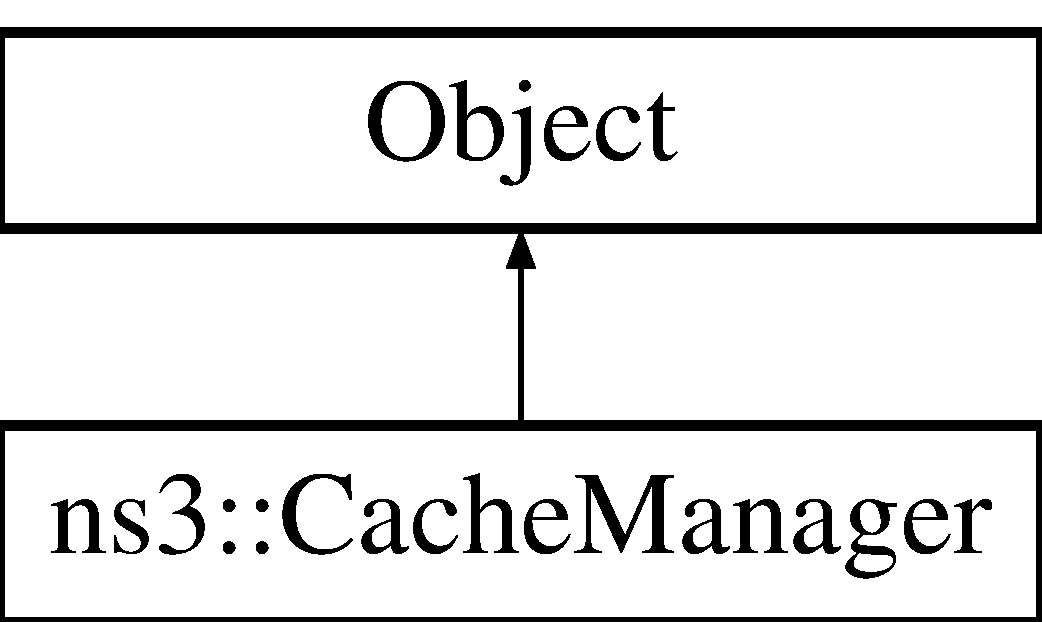
\includegraphics[height=2.000000cm]{classns3_1_1CacheManager}
\end{center}
\end{figure}
\subsection*{Public Member Functions}
\begin{DoxyCompactItemize}
\item 
\hyperlink{classns3_1_1CacheManager_a48853b4bb253bcc6c41c9185f8c81169}{Cache\-Manager} ()
\item 
virtual \hyperlink{classns3_1_1CacheManager_a6c35578ef0c60fc2395a813d5c26c395}{$\sim$\-Cache\-Manager} ()
\item 
void \hyperlink{classns3_1_1CacheManager_a154c3d0f83d4ad2cf3960017f5e26577}{Set\-Node} (Ptr$<$ Node $>$ node)
\begin{DoxyCompactList}\small\item\em Set node associated with this stack. \end{DoxyCompactList}\item 
Ptr$<$ Node $>$ \hyperlink{classns3_1_1CacheManager_a124af97c5ed58b4df52f0f9db827c6ab}{Get\-Node} ()
\begin{DoxyCompactList}\small\item\em Get node associated with this stack. \end{DoxyCompactList}\item 
bool \hyperlink{classns3_1_1CacheManager_ac07096eecd5c92c16ff0e68b1a9acf0b}{Set\-Entry} (Ptr$<$ Packet $>$ packet, std\-::string name, Ipv4\-Header ipheader)
\begin{DoxyCompactList}\small\item\em Creates a cache entry from the data of the packet and stores it in the Cache. It also creates an index for the content and stores it in the Policy\-Index. All these are achieved by calling the appropriate functions in Named \hyperlink{classns3_1_1Content}{Content} Cache class. \end{DoxyCompactList}\end{DoxyCompactItemize}
\subsection*{Static Public Member Functions}
\begin{DoxyCompactItemize}
\item 
static Type\-Id \hyperlink{classns3_1_1CacheManager_ac9b2923c1cbddb3868245fd3e0983159}{Get\-Type\-Id} (void)
\begin{DoxyCompactList}\small\item\em Get the type I\-D. \end{DoxyCompactList}\end{DoxyCompactItemize}
\subsection*{Private Attributes}
\begin{DoxyCompactItemize}
\item 
Ptr$<$ Node $>$ \hyperlink{classns3_1_1CacheManager_acc6de7f84389b36268a9124a5f6b03d8}{m\-\_\-node}
\end{DoxyCompactItemize}


\subsection{Detailed Description}
Manages the Named \hyperlink{classns3_1_1Content}{Content} Cache of an O\-I\-C\-N Router. 

This class takes care of the insertion and eviction process of the Cache and Policy\-Index through the functions of Named \hyperlink{classns3_1_1Content}{Content} Cache class. It also acts as an Interface between I\-C\-N Manager and O\-I\-C\-N Router when I\-C\-N Manager has to request a particular O\-I\-C\-N Router to retrieve a queried content from its cache. The Cache Manager then find the queried content through its name from the cache, creates a packet and sends it down the stack to \hyperlink{classns3_1_1SublayerProtocol}{Sublayer\-Protocol} class.

This class is instantiated and aggregated to all O\-I\-C\-N Routers in the network, and is not required in any other components of O\-I\-C\-N Architecture.

Note\-: The word Cache here refers to the boost\-::unordered\-\_\-map that stores the content along with its corresponding name. The word Policy\-Index refers to the boost\-::bimap container used for indexing the stored content in Cache. 

\subsection{Constructor \& Destructor Documentation}
\hypertarget{classns3_1_1CacheManager_a48853b4bb253bcc6c41c9185f8c81169}{\index{ns3\-::\-Cache\-Manager@{ns3\-::\-Cache\-Manager}!Cache\-Manager@{Cache\-Manager}}
\index{Cache\-Manager@{Cache\-Manager}!ns3::CacheManager@{ns3\-::\-Cache\-Manager}}
\subsubsection[{Cache\-Manager}]{\setlength{\rightskip}{0pt plus 5cm}ns3\-::\-Cache\-Manager\-::\-Cache\-Manager (
\begin{DoxyParamCaption}
{}
\end{DoxyParamCaption}
)}}\label{classns3_1_1CacheManager_a48853b4bb253bcc6c41c9185f8c81169}
\hypertarget{classns3_1_1CacheManager_a6c35578ef0c60fc2395a813d5c26c395}{\index{ns3\-::\-Cache\-Manager@{ns3\-::\-Cache\-Manager}!$\sim$\-Cache\-Manager@{$\sim$\-Cache\-Manager}}
\index{$\sim$\-Cache\-Manager@{$\sim$\-Cache\-Manager}!ns3::CacheManager@{ns3\-::\-Cache\-Manager}}
\subsubsection[{$\sim$\-Cache\-Manager}]{\setlength{\rightskip}{0pt plus 5cm}ns3\-::\-Cache\-Manager\-::$\sim$\-Cache\-Manager (
\begin{DoxyParamCaption}
{}
\end{DoxyParamCaption}
)\hspace{0.3cm}{\ttfamily [virtual]}}}\label{classns3_1_1CacheManager_a6c35578ef0c60fc2395a813d5c26c395}


\subsection{Member Function Documentation}
\hypertarget{classns3_1_1CacheManager_a124af97c5ed58b4df52f0f9db827c6ab}{\index{ns3\-::\-Cache\-Manager@{ns3\-::\-Cache\-Manager}!Get\-Node@{Get\-Node}}
\index{Get\-Node@{Get\-Node}!ns3::CacheManager@{ns3\-::\-Cache\-Manager}}
\subsubsection[{Get\-Node}]{\setlength{\rightskip}{0pt plus 5cm}Ptr$<$ Node $>$ ns3\-::\-Cache\-Manager\-::\-Get\-Node (
\begin{DoxyParamCaption}
{}
\end{DoxyParamCaption}
)}}\label{classns3_1_1CacheManager_a124af97c5ed58b4df52f0f9db827c6ab}


Get node associated with this stack. 

\begin{DoxyReturn}{Returns}
node of the stack 
\end{DoxyReturn}
\hypertarget{classns3_1_1CacheManager_ac9b2923c1cbddb3868245fd3e0983159}{\index{ns3\-::\-Cache\-Manager@{ns3\-::\-Cache\-Manager}!Get\-Type\-Id@{Get\-Type\-Id}}
\index{Get\-Type\-Id@{Get\-Type\-Id}!ns3::CacheManager@{ns3\-::\-Cache\-Manager}}
\subsubsection[{Get\-Type\-Id}]{\setlength{\rightskip}{0pt plus 5cm}Type\-Id ns3\-::\-Cache\-Manager\-::\-Get\-Type\-Id (
\begin{DoxyParamCaption}
\item[{void}]{}
\end{DoxyParamCaption}
)\hspace{0.3cm}{\ttfamily [static]}}}\label{classns3_1_1CacheManager_ac9b2923c1cbddb3868245fd3e0983159}


Get the type I\-D. 

\begin{DoxyReturn}{Returns}
the object Type\-Id 
\end{DoxyReturn}
\hypertarget{classns3_1_1CacheManager_ac07096eecd5c92c16ff0e68b1a9acf0b}{\index{ns3\-::\-Cache\-Manager@{ns3\-::\-Cache\-Manager}!Set\-Entry@{Set\-Entry}}
\index{Set\-Entry@{Set\-Entry}!ns3::CacheManager@{ns3\-::\-Cache\-Manager}}
\subsubsection[{Set\-Entry}]{\setlength{\rightskip}{0pt plus 5cm}bool ns3\-::\-Cache\-Manager\-::\-Set\-Entry (
\begin{DoxyParamCaption}
\item[{Ptr$<$ Packet $>$}]{packet, }
\item[{std\-::string}]{name, }
\item[{Ipv4\-Header}]{ipheader}
\end{DoxyParamCaption}
)}}\label{classns3_1_1CacheManager_ac07096eecd5c92c16ff0e68b1a9acf0b}


Creates a cache entry from the data of the packet and stores it in the Cache. It also creates an index for the content and stores it in the Policy\-Index. All these are achieved by calling the appropriate functions in Named \hyperlink{classns3_1_1Content}{Content} Cache class. 


\begin{DoxyParams}{Parameters}
{\em packet} & packet received by O\-I\-C\-N Router \\
\hline
{\em name} & name of the content present in the packet \\
\hline
{\em ipheader} & ip header of the packet \\
\hline
\end{DoxyParams}
\begin{DoxyReturn}{Returns}
true if the content is cached 
\end{DoxyReturn}
\hypertarget{classns3_1_1CacheManager_a154c3d0f83d4ad2cf3960017f5e26577}{\index{ns3\-::\-Cache\-Manager@{ns3\-::\-Cache\-Manager}!Set\-Node@{Set\-Node}}
\index{Set\-Node@{Set\-Node}!ns3::CacheManager@{ns3\-::\-Cache\-Manager}}
\subsubsection[{Set\-Node}]{\setlength{\rightskip}{0pt plus 5cm}void ns3\-::\-Cache\-Manager\-::\-Set\-Node (
\begin{DoxyParamCaption}
\item[{Ptr$<$ Node $>$}]{node}
\end{DoxyParamCaption}
)}}\label{classns3_1_1CacheManager_a154c3d0f83d4ad2cf3960017f5e26577}


Set node associated with this stack. 


\begin{DoxyParams}{Parameters}
{\em node} & node to set \\
\hline
\end{DoxyParams}


\subsection{Member Data Documentation}
\hypertarget{classns3_1_1CacheManager_acc6de7f84389b36268a9124a5f6b03d8}{\index{ns3\-::\-Cache\-Manager@{ns3\-::\-Cache\-Manager}!m\-\_\-node@{m\-\_\-node}}
\index{m\-\_\-node@{m\-\_\-node}!ns3::CacheManager@{ns3\-::\-Cache\-Manager}}
\subsubsection[{m\-\_\-node}]{\setlength{\rightskip}{0pt plus 5cm}Ptr$<$Node$>$ ns3\-::\-Cache\-Manager\-::m\-\_\-node\hspace{0.3cm}{\ttfamily [private]}}}\label{classns3_1_1CacheManager_acc6de7f84389b36268a9124a5f6b03d8}


The documentation for this class was generated from the following files\-:\begin{DoxyCompactItemize}
\item 
model/\hyperlink{cache-manager_8h}{cache-\/manager.\-h}\item 
model/\hyperlink{cache-manager_8cc}{cache-\/manager.\-cc}\end{DoxyCompactItemize}

\hypertarget{classns3_1_1CacheWithFifo}{\section{ns3\-:\-:Cache\-With\-Fifo Class Reference}
\label{classns3_1_1CacheWithFifo}\index{ns3\-::\-Cache\-With\-Fifo@{ns3\-::\-Cache\-With\-Fifo}}
}


This class implements the first in first out caching policy.  




{\ttfamily \#include $<$cache-\/with-\/fifo.\-h$>$}

Inheritance diagram for ns3\-:\-:Cache\-With\-Fifo\-:\begin{figure}[H]
\begin{center}
\leavevmode
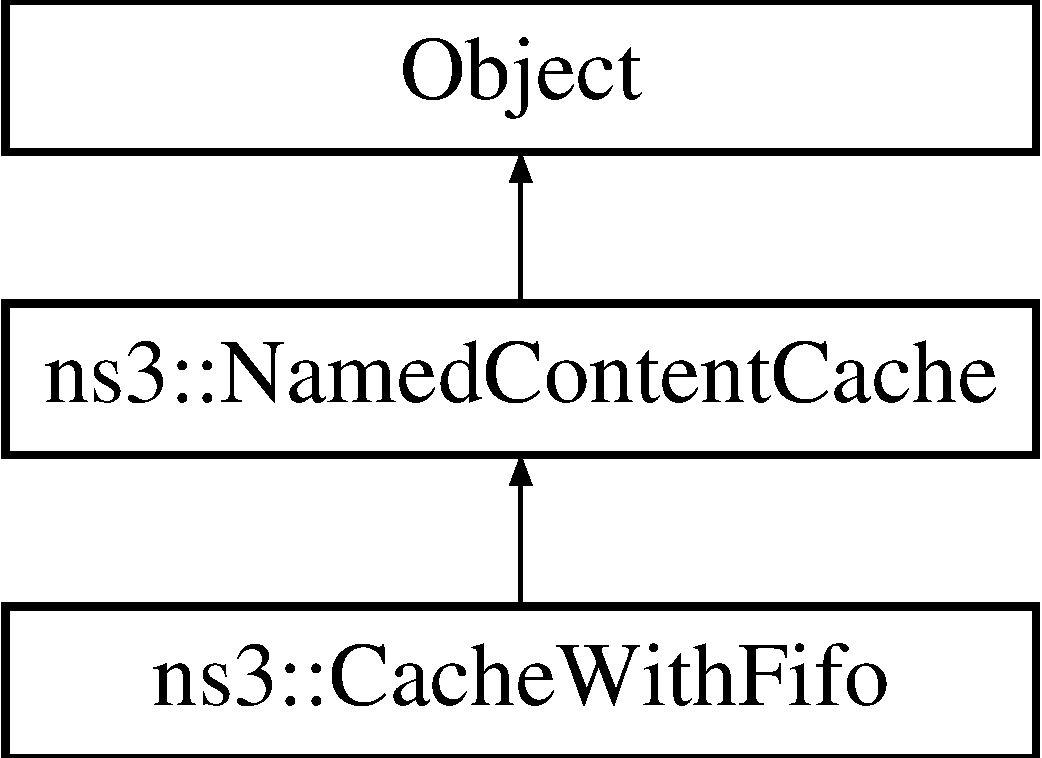
\includegraphics[height=3.000000cm]{classns3_1_1CacheWithFifo}
\end{center}
\end{figure}
\subsection*{Public Member Functions}
\begin{DoxyCompactItemize}
\item 
\hyperlink{classns3_1_1CacheWithFifo_a1171d394f7f60439263b8b2dedfa8ff5}{Cache\-With\-Fifo} ()
\item 
virtual \hyperlink{classns3_1_1CacheWithFifo_aa2665a704001cdde625684a23eb95177}{$\sim$\-Cache\-With\-Fifo} ()
\item 
virtual void \hyperlink{classns3_1_1CacheWithFifo_a6e92a91f36ac87a001644e299be4dd41}{Set\-Cache\-Size} (uint32\-\_\-t size)
\begin{DoxyCompactList}\small\item\em Set the cache size of the Cache. \end{DoxyCompactList}\item 
virtual uint32\-\_\-t \hyperlink{classns3_1_1CacheWithFifo_ae94f385620f20825ad07995dccc8075a}{Get\-Cache\-Size} (void)
\begin{DoxyCompactList}\small\item\em Get the cache size of the Cache. \end{DoxyCompactList}\item 
virtual void \hyperlink{classns3_1_1CacheWithFifo_a7ad5dd349c8ea2633d6c60c0fb5e43ea}{Set\-Freshness\-Time} (uint64\-\_\-t time)
\begin{DoxyCompactList}\small\item\em Set the freshness time for the contents of Cache. \end{DoxyCompactList}\item 
virtual uint64\-\_\-t \hyperlink{classns3_1_1CacheWithFifo_aa56864aee34859897793284eb7c7f9db}{Get\-Freshness\-Time} (void)
\begin{DoxyCompactList}\small\item\em Get the freshness time set for the contents of Cache. \end{DoxyCompactList}\item 
virtual \hyperlink{classns3_1_1NamedContentCacheEntry}{Named\-Content\-Cache\-Entry} \hyperlink{classns3_1_1CacheWithFifo_ae9be9920ddca0d7a001a054381c0543c}{Create\-Entry} (std\-::string Name, Ptr$<$ Packet $>$ packet, Ipv4\-Header ipheader)
\begin{DoxyCompactList}\small\item\em Create the Cache entry, which is an object of \hyperlink{classns3_1_1NamedContentCacheEntry}{Named\-Content\-Cache\-Entry} class. The subclasses will define this function to create an entry that has the requisite parameters of the content, for the purpose of indexing content according to caching policy the subclass represents. \end{DoxyCompactList}\item 
virtual uint32\-\_\-t \hyperlink{classns3_1_1CacheWithFifo_a15c2b5cf0e52e8da5fbd4d7e32d0aedc}{Create\-Index} (\hyperlink{classns3_1_1NamedContentCacheEntry}{Named\-Content\-Cache\-Entry} entry)
\begin{DoxyCompactList}\small\item\em Create the index of the corresponding entry, by using the parameters of the content present in the entry class. The subclasses will define this function to create an index which, when put in order, will arrange the contents according to the caching policy the subclass represents. If some subclasses need decimal indexes, they have to multiply the obtained index with a factor to ensure unique integer indexes are obtained. \end{DoxyCompactList}\item 
virtual void \hyperlink{classns3_1_1CacheWithFifo_a2b0a3e5d4d83775f99e6a453bbb9f764}{Insert\-To\-Cache} (std\-::string Name, \hyperlink{classns3_1_1NamedContentCacheEntry}{Named\-Content\-Cache\-Entry} entry)
\begin{DoxyCompactList}\small\item\em Insert the Name of the content and its corresponding entry object to the Cache. \end{DoxyCompactList}\item 
virtual void \hyperlink{classns3_1_1CacheWithFifo_a2f6375a96e425628f4ef48df89fc2319}{Insert\-To\-Policy\-Index} (uint32\-\_\-t index, std\-::string Name)
\begin{DoxyCompactList}\small\item\em Insert the index of the content and its corresponding name to the Policy\-Index. \end{DoxyCompactList}\item 
virtual bool \hyperlink{classns3_1_1CacheWithFifo_a15468a5d2fc215b32a8e531944c4197e}{Is\-Full} (void)
\begin{DoxyCompactList}\small\item\em Check if the Cache is full, i.\-e. if the number of contents is equal the cache size. \end{DoxyCompactList}\item 
virtual bool \hyperlink{classns3_1_1CacheWithFifo_a90d9c0afe3ef2579dd6faf1f70aeb4e0}{Is\-Unique} (std\-::string Name)
\begin{DoxyCompactList}\small\item\em it check whether content is present in the cache or not \end{DoxyCompactList}\item 
virtual bool \hyperlink{classns3_1_1CacheWithFifo_a69b633b7e17cb8f13e7a66afb942a258}{Is\-Evictable} (uint32\-\_\-t index)
\begin{DoxyCompactList}\small\item\em Check if the content with the given index can be inserted with the eviction of some other content when the is full. The new content can be inserted if its index is lesser than (or greater than, when arranged in descending order) the first content, or if any content's freshness has expired. Some caching policies, like F\-I\-F\-O, keep on inserting new content, irrespective of its index. Subclasses representing such policies need not define and use this function. \end{DoxyCompactList}\item 
virtual std\-::string \hyperlink{classns3_1_1CacheWithFifo_a3440b3cf70e24dd33d511656c0d77112}{Evict\-Entry} (void)
\begin{DoxyCompactList}\small\item\em Evict the first content in Policy\-Index and also the corresponding entry in the Cache. This is the main eviction function of \hyperlink{classns3_1_1NamedContentCache}{Named\-Content\-Cache}. \end{DoxyCompactList}\item 
virtual void \hyperlink{classns3_1_1CacheWithFifo_a156013f129c1d13538ed92e6116a2d20}{Evict\-Entry} (std\-::string Name)
\begin{DoxyCompactList}\small\item\em Evict the content with corresponding name from both Policy\-Index and Cache. This has to be done when a packet having a content that already exists in the Cache has been received the I\-C\-N Router. This operation basically evicts the older entry of the same content so that the newer entry can be inserted. This function has to be defined by all subclasses because every content name in Cache and Policy\-Index has to be unique. \end{DoxyCompactList}\item 
virtual Ptr$<$ Packet $>$ \hyperlink{classns3_1_1CacheWithFifo_a36311448f4cef69aa4be77dfc91eb3d5}{Find} (std\-::string Name)
\begin{DoxyCompactList}\small\item\em Find the content with given name in the Cache. \end{DoxyCompactList}\item 
virtual void \hyperlink{classns3_1_1CacheWithFifo_ae3b39d8b8187650d19806a8950ea9515}{Update\-Index} (std\-::string Name)
\begin{DoxyCompactList}\small\item\em Update the index of the content with the given name. This has to be done when the content is retrieved from Cache to be sent to a querying O\-I\-C\-N Client. The subclasses will define this function based on the requirements of the caching policies they represent. \end{DoxyCompactList}\end{DoxyCompactItemize}
\subsection*{Static Public Member Functions}
\begin{DoxyCompactItemize}
\item 
static Type\-Id \hyperlink{classns3_1_1CacheWithFifo_af0d8c81ef307fb573d5132fdb70500a6}{Get\-Type\-Id} (void)
\end{DoxyCompactItemize}
\subsection*{Private Attributes}
\begin{DoxyCompactItemize}
\item 
uint32\-\_\-t \hyperlink{classns3_1_1CacheWithFifo_a73682581680dbb344b2d39fcec84d22a}{cache\-\_\-size}
\begin{DoxyCompactList}\small\item\em size of the Cache \end{DoxyCompactList}\item 
\hyperlink{classns3_1_1NamedContentCache_a9aa35d883b9f4153d97b6e7dc74f9307}{Cache} \hyperlink{classns3_1_1CacheWithFifo_a0156478153f80ff4c9980c8ad41a5c6e}{cache}
\begin{DoxyCompactList}\small\item\em the main cache container which stores the name and corresponding content \end{DoxyCompactList}\item 
\hyperlink{classns3_1_1NamedContentCache_a0b728ea2d4e0acbe431897b2374cfc8e}{Policy\-Index} \hyperlink{classns3_1_1CacheWithFifo_a6eac664460d6029cebf941cd42097d0b}{policyindex}
\begin{DoxyCompactList}\small\item\em policy indexed container, containing index and content name \end{DoxyCompactList}\end{DoxyCompactItemize}
\subsection*{Additional Inherited Members}


\subsection{Detailed Description}
This class implements the first in first out caching policy. 

\subsection{Constructor \& Destructor Documentation}
\hypertarget{classns3_1_1CacheWithFifo_a1171d394f7f60439263b8b2dedfa8ff5}{\index{ns3\-::\-Cache\-With\-Fifo@{ns3\-::\-Cache\-With\-Fifo}!Cache\-With\-Fifo@{Cache\-With\-Fifo}}
\index{Cache\-With\-Fifo@{Cache\-With\-Fifo}!ns3::CacheWithFifo@{ns3\-::\-Cache\-With\-Fifo}}
\subsubsection[{Cache\-With\-Fifo}]{\setlength{\rightskip}{0pt plus 5cm}ns3\-::\-Cache\-With\-Fifo\-::\-Cache\-With\-Fifo (
\begin{DoxyParamCaption}
{}
\end{DoxyParamCaption}
)}}\label{classns3_1_1CacheWithFifo_a1171d394f7f60439263b8b2dedfa8ff5}
\hypertarget{classns3_1_1CacheWithFifo_aa2665a704001cdde625684a23eb95177}{\index{ns3\-::\-Cache\-With\-Fifo@{ns3\-::\-Cache\-With\-Fifo}!$\sim$\-Cache\-With\-Fifo@{$\sim$\-Cache\-With\-Fifo}}
\index{$\sim$\-Cache\-With\-Fifo@{$\sim$\-Cache\-With\-Fifo}!ns3::CacheWithFifo@{ns3\-::\-Cache\-With\-Fifo}}
\subsubsection[{$\sim$\-Cache\-With\-Fifo}]{\setlength{\rightskip}{0pt plus 5cm}ns3\-::\-Cache\-With\-Fifo\-::$\sim$\-Cache\-With\-Fifo (
\begin{DoxyParamCaption}
{}
\end{DoxyParamCaption}
)\hspace{0.3cm}{\ttfamily [virtual]}}}\label{classns3_1_1CacheWithFifo_aa2665a704001cdde625684a23eb95177}


\subsection{Member Function Documentation}
\hypertarget{classns3_1_1CacheWithFifo_ae9be9920ddca0d7a001a054381c0543c}{\index{ns3\-::\-Cache\-With\-Fifo@{ns3\-::\-Cache\-With\-Fifo}!Create\-Entry@{Create\-Entry}}
\index{Create\-Entry@{Create\-Entry}!ns3::CacheWithFifo@{ns3\-::\-Cache\-With\-Fifo}}
\subsubsection[{Create\-Entry}]{\setlength{\rightskip}{0pt plus 5cm}{\bf Named\-Content\-Cache\-Entry} ns3\-::\-Cache\-With\-Fifo\-::\-Create\-Entry (
\begin{DoxyParamCaption}
\item[{std\-::string}]{Name, }
\item[{Ptr$<$ Packet $>$}]{packet, }
\item[{Ipv4\-Header}]{ipheader}
\end{DoxyParamCaption}
)\hspace{0.3cm}{\ttfamily [virtual]}}}\label{classns3_1_1CacheWithFifo_ae9be9920ddca0d7a001a054381c0543c}


Create the Cache entry, which is an object of \hyperlink{classns3_1_1NamedContentCacheEntry}{Named\-Content\-Cache\-Entry} class. The subclasses will define this function to create an entry that has the requisite parameters of the content, for the purpose of indexing content according to caching policy the subclass represents. 


\begin{DoxyParams}{Parameters}
{\em Name} & name of the content \\
\hline
{\em packet} & packet received by I\-C\-N Router, with its I\-P, Transport and O\-I\-C\-N headers removed \\
\hline
{\em ipheader} & I\-P Header of the packet, from which the required parameters of the content (present in packet) can retrieved. \\
\hline
\end{DoxyParams}
\begin{DoxyReturn}{Returns}
the newly created cache entry 
\end{DoxyReturn}


Implements \hyperlink{classns3_1_1NamedContentCache_a154317526b3883db729c365ab342074a}{ns3\-::\-Named\-Content\-Cache}.

\hypertarget{classns3_1_1CacheWithFifo_a15c2b5cf0e52e8da5fbd4d7e32d0aedc}{\index{ns3\-::\-Cache\-With\-Fifo@{ns3\-::\-Cache\-With\-Fifo}!Create\-Index@{Create\-Index}}
\index{Create\-Index@{Create\-Index}!ns3::CacheWithFifo@{ns3\-::\-Cache\-With\-Fifo}}
\subsubsection[{Create\-Index}]{\setlength{\rightskip}{0pt plus 5cm}uint32\-\_\-t ns3\-::\-Cache\-With\-Fifo\-::\-Create\-Index (
\begin{DoxyParamCaption}
\item[{{\bf Named\-Content\-Cache\-Entry}}]{entry}
\end{DoxyParamCaption}
)\hspace{0.3cm}{\ttfamily [virtual]}}}\label{classns3_1_1CacheWithFifo_a15c2b5cf0e52e8da5fbd4d7e32d0aedc}


Create the index of the corresponding entry, by using the parameters of the content present in the entry class. The subclasses will define this function to create an index which, when put in order, will arrange the contents according to the caching policy the subclass represents. If some subclasses need decimal indexes, they have to multiply the obtained index with a factor to ensure unique integer indexes are obtained. 


\begin{DoxyParams}{Parameters}
{\em entry} & the cache entry corresponding to the content \\
\hline
\end{DoxyParams}
\begin{DoxyReturn}{Returns}
the newly created integer index for the content 
\end{DoxyReturn}


Implements \hyperlink{classns3_1_1NamedContentCache_a75be49c2ad5db93bdf8aaed813dcf304}{ns3\-::\-Named\-Content\-Cache}.

\hypertarget{classns3_1_1CacheWithFifo_a3440b3cf70e24dd33d511656c0d77112}{\index{ns3\-::\-Cache\-With\-Fifo@{ns3\-::\-Cache\-With\-Fifo}!Evict\-Entry@{Evict\-Entry}}
\index{Evict\-Entry@{Evict\-Entry}!ns3::CacheWithFifo@{ns3\-::\-Cache\-With\-Fifo}}
\subsubsection[{Evict\-Entry}]{\setlength{\rightskip}{0pt plus 5cm}std\-::string ns3\-::\-Cache\-With\-Fifo\-::\-Evict\-Entry (
\begin{DoxyParamCaption}
\item[{void}]{}
\end{DoxyParamCaption}
)\hspace{0.3cm}{\ttfamily [virtual]}}}\label{classns3_1_1CacheWithFifo_a3440b3cf70e24dd33d511656c0d77112}


Evict the first content in Policy\-Index and also the corresponding entry in the Cache. This is the main eviction function of \hyperlink{classns3_1_1NamedContentCache}{Named\-Content\-Cache}. 

\begin{DoxyReturn}{Returns}
the name of the evicted content 
\end{DoxyReturn}


Implements \hyperlink{classns3_1_1NamedContentCache_a87850f01fc632ede64af75d7c20f7a7e}{ns3\-::\-Named\-Content\-Cache}.

\hypertarget{classns3_1_1CacheWithFifo_a156013f129c1d13538ed92e6116a2d20}{\index{ns3\-::\-Cache\-With\-Fifo@{ns3\-::\-Cache\-With\-Fifo}!Evict\-Entry@{Evict\-Entry}}
\index{Evict\-Entry@{Evict\-Entry}!ns3::CacheWithFifo@{ns3\-::\-Cache\-With\-Fifo}}
\subsubsection[{Evict\-Entry}]{\setlength{\rightskip}{0pt plus 5cm}void ns3\-::\-Cache\-With\-Fifo\-::\-Evict\-Entry (
\begin{DoxyParamCaption}
\item[{std\-::string}]{Name}
\end{DoxyParamCaption}
)\hspace{0.3cm}{\ttfamily [virtual]}}}\label{classns3_1_1CacheWithFifo_a156013f129c1d13538ed92e6116a2d20}


Evict the content with corresponding name from both Policy\-Index and Cache. This has to be done when a packet having a content that already exists in the Cache has been received the I\-C\-N Router. This operation basically evicts the older entry of the same content so that the newer entry can be inserted. This function has to be defined by all subclasses because every content name in Cache and Policy\-Index has to be unique. 


\begin{DoxyParams}{Parameters}
{\em name} & name of the non-\/unique content \\
\hline
\end{DoxyParams}


Implements \hyperlink{classns3_1_1NamedContentCache_a254f3c74475e104a615739fc7577296f}{ns3\-::\-Named\-Content\-Cache}.

\hypertarget{classns3_1_1CacheWithFifo_a36311448f4cef69aa4be77dfc91eb3d5}{\index{ns3\-::\-Cache\-With\-Fifo@{ns3\-::\-Cache\-With\-Fifo}!Find@{Find}}
\index{Find@{Find}!ns3::CacheWithFifo@{ns3\-::\-Cache\-With\-Fifo}}
\subsubsection[{Find}]{\setlength{\rightskip}{0pt plus 5cm}Ptr$<$ Packet $>$ ns3\-::\-Cache\-With\-Fifo\-::\-Find (
\begin{DoxyParamCaption}
\item[{std\-::string}]{Name}
\end{DoxyParamCaption}
)\hspace{0.3cm}{\ttfamily [virtual]}}}\label{classns3_1_1CacheWithFifo_a36311448f4cef69aa4be77dfc91eb3d5}


Find the content with given name in the Cache. 

\begin{DoxyReturn}{Returns}
the content in the form of an Application Layer packet 
\end{DoxyReturn}


Implements \hyperlink{classns3_1_1NamedContentCache_a081439cd96d09e2f9f158f3aebe9fd7c}{ns3\-::\-Named\-Content\-Cache}.

\hypertarget{classns3_1_1CacheWithFifo_ae94f385620f20825ad07995dccc8075a}{\index{ns3\-::\-Cache\-With\-Fifo@{ns3\-::\-Cache\-With\-Fifo}!Get\-Cache\-Size@{Get\-Cache\-Size}}
\index{Get\-Cache\-Size@{Get\-Cache\-Size}!ns3::CacheWithFifo@{ns3\-::\-Cache\-With\-Fifo}}
\subsubsection[{Get\-Cache\-Size}]{\setlength{\rightskip}{0pt plus 5cm}uint32\-\_\-t ns3\-::\-Cache\-With\-Fifo\-::\-Get\-Cache\-Size (
\begin{DoxyParamCaption}
\item[{void}]{}
\end{DoxyParamCaption}
)\hspace{0.3cm}{\ttfamily [virtual]}}}\label{classns3_1_1CacheWithFifo_ae94f385620f20825ad07995dccc8075a}


Get the cache size of the Cache. 

\begin{DoxyReturn}{Returns}
the cache size of the Cache 
\end{DoxyReturn}


Implements \hyperlink{classns3_1_1NamedContentCache_afd9ade17d87082a46cbb745fd0196ab4}{ns3\-::\-Named\-Content\-Cache}.

\hypertarget{classns3_1_1CacheWithFifo_aa56864aee34859897793284eb7c7f9db}{\index{ns3\-::\-Cache\-With\-Fifo@{ns3\-::\-Cache\-With\-Fifo}!Get\-Freshness\-Time@{Get\-Freshness\-Time}}
\index{Get\-Freshness\-Time@{Get\-Freshness\-Time}!ns3::CacheWithFifo@{ns3\-::\-Cache\-With\-Fifo}}
\subsubsection[{Get\-Freshness\-Time}]{\setlength{\rightskip}{0pt plus 5cm}uint64\-\_\-t ns3\-::\-Cache\-With\-Fifo\-::\-Get\-Freshness\-Time (
\begin{DoxyParamCaption}
\item[{void}]{}
\end{DoxyParamCaption}
)\hspace{0.3cm}{\ttfamily [virtual]}}}\label{classns3_1_1CacheWithFifo_aa56864aee34859897793284eb7c7f9db}


Get the freshness time set for the contents of Cache. 

\begin{DoxyReturn}{Returns}
the freshness time in milliseconds 
\end{DoxyReturn}


Implements \hyperlink{classns3_1_1NamedContentCache_ac2b0e616d4e866cb2328e986f2ef69e1}{ns3\-::\-Named\-Content\-Cache}.

\hypertarget{classns3_1_1CacheWithFifo_af0d8c81ef307fb573d5132fdb70500a6}{\index{ns3\-::\-Cache\-With\-Fifo@{ns3\-::\-Cache\-With\-Fifo}!Get\-Type\-Id@{Get\-Type\-Id}}
\index{Get\-Type\-Id@{Get\-Type\-Id}!ns3::CacheWithFifo@{ns3\-::\-Cache\-With\-Fifo}}
\subsubsection[{Get\-Type\-Id}]{\setlength{\rightskip}{0pt plus 5cm}Type\-Id ns3\-::\-Cache\-With\-Fifo\-::\-Get\-Type\-Id (
\begin{DoxyParamCaption}
\item[{void}]{}
\end{DoxyParamCaption}
)\hspace{0.3cm}{\ttfamily [static]}}}\label{classns3_1_1CacheWithFifo_af0d8c81ef307fb573d5132fdb70500a6}
\hypertarget{classns3_1_1CacheWithFifo_a2b0a3e5d4d83775f99e6a453bbb9f764}{\index{ns3\-::\-Cache\-With\-Fifo@{ns3\-::\-Cache\-With\-Fifo}!Insert\-To\-Cache@{Insert\-To\-Cache}}
\index{Insert\-To\-Cache@{Insert\-To\-Cache}!ns3::CacheWithFifo@{ns3\-::\-Cache\-With\-Fifo}}
\subsubsection[{Insert\-To\-Cache}]{\setlength{\rightskip}{0pt plus 5cm}void ns3\-::\-Cache\-With\-Fifo\-::\-Insert\-To\-Cache (
\begin{DoxyParamCaption}
\item[{std\-::string}]{Name, }
\item[{{\bf Named\-Content\-Cache\-Entry}}]{entry}
\end{DoxyParamCaption}
)\hspace{0.3cm}{\ttfamily [virtual]}}}\label{classns3_1_1CacheWithFifo_a2b0a3e5d4d83775f99e6a453bbb9f764}


Insert the Name of the content and its corresponding entry object to the Cache. 


\begin{DoxyParams}{Parameters}
{\em Name} & name of the content \\
\hline
{\em entry} & the cache entry corresponding to the content \\
\hline
\end{DoxyParams}


Implements \hyperlink{classns3_1_1NamedContentCache_a56a23add9b5bc03908793cf261ccb5f8}{ns3\-::\-Named\-Content\-Cache}.

\hypertarget{classns3_1_1CacheWithFifo_a2f6375a96e425628f4ef48df89fc2319}{\index{ns3\-::\-Cache\-With\-Fifo@{ns3\-::\-Cache\-With\-Fifo}!Insert\-To\-Policy\-Index@{Insert\-To\-Policy\-Index}}
\index{Insert\-To\-Policy\-Index@{Insert\-To\-Policy\-Index}!ns3::CacheWithFifo@{ns3\-::\-Cache\-With\-Fifo}}
\subsubsection[{Insert\-To\-Policy\-Index}]{\setlength{\rightskip}{0pt plus 5cm}void ns3\-::\-Cache\-With\-Fifo\-::\-Insert\-To\-Policy\-Index (
\begin{DoxyParamCaption}
\item[{uint32\-\_\-t}]{index, }
\item[{std\-::string}]{Name}
\end{DoxyParamCaption}
)\hspace{0.3cm}{\ttfamily [virtual]}}}\label{classns3_1_1CacheWithFifo_a2f6375a96e425628f4ef48df89fc2319}


Insert the index of the content and its corresponding name to the Policy\-Index. 


\begin{DoxyParams}{Parameters}
{\em index} & the unique integer index of the content \\
\hline
{\em Name} & name of the content \\
\hline
\end{DoxyParams}


Implements \hyperlink{classns3_1_1NamedContentCache_ac248e647f56a6fef10285b1c654b8180}{ns3\-::\-Named\-Content\-Cache}.

\hypertarget{classns3_1_1CacheWithFifo_a69b633b7e17cb8f13e7a66afb942a258}{\index{ns3\-::\-Cache\-With\-Fifo@{ns3\-::\-Cache\-With\-Fifo}!Is\-Evictable@{Is\-Evictable}}
\index{Is\-Evictable@{Is\-Evictable}!ns3::CacheWithFifo@{ns3\-::\-Cache\-With\-Fifo}}
\subsubsection[{Is\-Evictable}]{\setlength{\rightskip}{0pt plus 5cm}bool ns3\-::\-Cache\-With\-Fifo\-::\-Is\-Evictable (
\begin{DoxyParamCaption}
\item[{uint32\-\_\-t}]{index}
\end{DoxyParamCaption}
)\hspace{0.3cm}{\ttfamily [virtual]}}}\label{classns3_1_1CacheWithFifo_a69b633b7e17cb8f13e7a66afb942a258}


Check if the content with the given index can be inserted with the eviction of some other content when the is full. The new content can be inserted if its index is lesser than (or greater than, when arranged in descending order) the first content, or if any content's freshness has expired. Some caching policies, like F\-I\-F\-O, keep on inserting new content, irrespective of its index. Subclasses representing such policies need not define and use this function. 


\begin{DoxyParams}{Parameters}
{\em index} & the unique integer index of the content \\
\hline
\end{DoxyParams}
\begin{DoxyReturn}{Returns}
true if any existing content can be evicted so that the new content with the given index can be inserted. 
\end{DoxyReturn}


Implements \hyperlink{classns3_1_1NamedContentCache_a281ad340f9771fa2ed898a1ad569d0da}{ns3\-::\-Named\-Content\-Cache}.

\hypertarget{classns3_1_1CacheWithFifo_a15468a5d2fc215b32a8e531944c4197e}{\index{ns3\-::\-Cache\-With\-Fifo@{ns3\-::\-Cache\-With\-Fifo}!Is\-Full@{Is\-Full}}
\index{Is\-Full@{Is\-Full}!ns3::CacheWithFifo@{ns3\-::\-Cache\-With\-Fifo}}
\subsubsection[{Is\-Full}]{\setlength{\rightskip}{0pt plus 5cm}bool ns3\-::\-Cache\-With\-Fifo\-::\-Is\-Full (
\begin{DoxyParamCaption}
\item[{void}]{}
\end{DoxyParamCaption}
)\hspace{0.3cm}{\ttfamily [virtual]}}}\label{classns3_1_1CacheWithFifo_a15468a5d2fc215b32a8e531944c4197e}


Check if the Cache is full, i.\-e. if the number of contents is equal the cache size. 

\begin{DoxyReturn}{Returns}
true if the Cache is full 
\end{DoxyReturn}


Implements \hyperlink{classns3_1_1NamedContentCache_a1ceeaf5b85d3571225adfe2d48caf126}{ns3\-::\-Named\-Content\-Cache}.

\hypertarget{classns3_1_1CacheWithFifo_a90d9c0afe3ef2579dd6faf1f70aeb4e0}{\index{ns3\-::\-Cache\-With\-Fifo@{ns3\-::\-Cache\-With\-Fifo}!Is\-Unique@{Is\-Unique}}
\index{Is\-Unique@{Is\-Unique}!ns3::CacheWithFifo@{ns3\-::\-Cache\-With\-Fifo}}
\subsubsection[{Is\-Unique}]{\setlength{\rightskip}{0pt plus 5cm}bool ns3\-::\-Cache\-With\-Fifo\-::\-Is\-Unique (
\begin{DoxyParamCaption}
\item[{std\-::string}]{name}
\end{DoxyParamCaption}
)\hspace{0.3cm}{\ttfamily [virtual]}}}\label{classns3_1_1CacheWithFifo_a90d9c0afe3ef2579dd6faf1f70aeb4e0}


it check whether content is present in the cache or not 


\begin{DoxyParams}{Parameters}
{\em name} & name of the content \\
\hline
\end{DoxyParams}
\begin{DoxyReturn}{Returns}
true if content is not present, false when content is present in the cache 
\end{DoxyReturn}


Implements \hyperlink{classns3_1_1NamedContentCache_a4c4a79310c99f9c8ad6227d3b380dc20}{ns3\-::\-Named\-Content\-Cache}.

\hypertarget{classns3_1_1CacheWithFifo_a6e92a91f36ac87a001644e299be4dd41}{\index{ns3\-::\-Cache\-With\-Fifo@{ns3\-::\-Cache\-With\-Fifo}!Set\-Cache\-Size@{Set\-Cache\-Size}}
\index{Set\-Cache\-Size@{Set\-Cache\-Size}!ns3::CacheWithFifo@{ns3\-::\-Cache\-With\-Fifo}}
\subsubsection[{Set\-Cache\-Size}]{\setlength{\rightskip}{0pt plus 5cm}void ns3\-::\-Cache\-With\-Fifo\-::\-Set\-Cache\-Size (
\begin{DoxyParamCaption}
\item[{uint32\-\_\-t}]{size}
\end{DoxyParamCaption}
)\hspace{0.3cm}{\ttfamily [virtual]}}}\label{classns3_1_1CacheWithFifo_a6e92a91f36ac87a001644e299be4dd41}


Set the cache size of the Cache. 


\begin{DoxyParams}{Parameters}
{\em size} & the size to which the cache has to be set \\
\hline
\end{DoxyParams}


Implements \hyperlink{classns3_1_1NamedContentCache_ae28605a03a5a4d8b9a3494b4068f44e2}{ns3\-::\-Named\-Content\-Cache}.

\hypertarget{classns3_1_1CacheWithFifo_a7ad5dd349c8ea2633d6c60c0fb5e43ea}{\index{ns3\-::\-Cache\-With\-Fifo@{ns3\-::\-Cache\-With\-Fifo}!Set\-Freshness\-Time@{Set\-Freshness\-Time}}
\index{Set\-Freshness\-Time@{Set\-Freshness\-Time}!ns3::CacheWithFifo@{ns3\-::\-Cache\-With\-Fifo}}
\subsubsection[{Set\-Freshness\-Time}]{\setlength{\rightskip}{0pt plus 5cm}void ns3\-::\-Cache\-With\-Fifo\-::\-Set\-Freshness\-Time (
\begin{DoxyParamCaption}
\item[{uint64\-\_\-t}]{time}
\end{DoxyParamCaption}
)\hspace{0.3cm}{\ttfamily [virtual]}}}\label{classns3_1_1CacheWithFifo_a7ad5dd349c8ea2633d6c60c0fb5e43ea}


Set the freshness time for the contents of Cache. 


\begin{DoxyParams}{Parameters}
{\em time} & the freshness time in milliseconds \\
\hline
\end{DoxyParams}


Implements \hyperlink{classns3_1_1NamedContentCache_a92a5e2e641a11d15300f621aa77275ab}{ns3\-::\-Named\-Content\-Cache}.

\hypertarget{classns3_1_1CacheWithFifo_ae3b39d8b8187650d19806a8950ea9515}{\index{ns3\-::\-Cache\-With\-Fifo@{ns3\-::\-Cache\-With\-Fifo}!Update\-Index@{Update\-Index}}
\index{Update\-Index@{Update\-Index}!ns3::CacheWithFifo@{ns3\-::\-Cache\-With\-Fifo}}
\subsubsection[{Update\-Index}]{\setlength{\rightskip}{0pt plus 5cm}void ns3\-::\-Cache\-With\-Fifo\-::\-Update\-Index (
\begin{DoxyParamCaption}
\item[{std\-::string}]{Name}
\end{DoxyParamCaption}
)\hspace{0.3cm}{\ttfamily [virtual]}}}\label{classns3_1_1CacheWithFifo_ae3b39d8b8187650d19806a8950ea9515}


Update the index of the content with the given name. This has to be done when the content is retrieved from Cache to be sent to a querying O\-I\-C\-N Client. The subclasses will define this function based on the requirements of the caching policies they represent. 


\begin{DoxyParams}{Parameters}
{\em the} & name of the content whose index has to be updated \\
\hline
\end{DoxyParams}


Implements \hyperlink{classns3_1_1NamedContentCache_aeabf8afacd89cbc46b78b382c8a487e8}{ns3\-::\-Named\-Content\-Cache}.



\subsection{Member Data Documentation}
\hypertarget{classns3_1_1CacheWithFifo_a0156478153f80ff4c9980c8ad41a5c6e}{\index{ns3\-::\-Cache\-With\-Fifo@{ns3\-::\-Cache\-With\-Fifo}!cache@{cache}}
\index{cache@{cache}!ns3::CacheWithFifo@{ns3\-::\-Cache\-With\-Fifo}}
\subsubsection[{cache}]{\setlength{\rightskip}{0pt plus 5cm}{\bf Cache} ns3\-::\-Cache\-With\-Fifo\-::cache\hspace{0.3cm}{\ttfamily [private]}}}\label{classns3_1_1CacheWithFifo_a0156478153f80ff4c9980c8ad41a5c6e}


the main cache container which stores the name and corresponding content 

\hypertarget{classns3_1_1CacheWithFifo_a73682581680dbb344b2d39fcec84d22a}{\index{ns3\-::\-Cache\-With\-Fifo@{ns3\-::\-Cache\-With\-Fifo}!cache\-\_\-size@{cache\-\_\-size}}
\index{cache\-\_\-size@{cache\-\_\-size}!ns3::CacheWithFifo@{ns3\-::\-Cache\-With\-Fifo}}
\subsubsection[{cache\-\_\-size}]{\setlength{\rightskip}{0pt plus 5cm}uint32\-\_\-t ns3\-::\-Cache\-With\-Fifo\-::cache\-\_\-size\hspace{0.3cm}{\ttfamily [private]}}}\label{classns3_1_1CacheWithFifo_a73682581680dbb344b2d39fcec84d22a}


size of the Cache 

\hypertarget{classns3_1_1CacheWithFifo_a6eac664460d6029cebf941cd42097d0b}{\index{ns3\-::\-Cache\-With\-Fifo@{ns3\-::\-Cache\-With\-Fifo}!policyindex@{policyindex}}
\index{policyindex@{policyindex}!ns3::CacheWithFifo@{ns3\-::\-Cache\-With\-Fifo}}
\subsubsection[{policyindex}]{\setlength{\rightskip}{0pt plus 5cm}{\bf Policy\-Index} ns3\-::\-Cache\-With\-Fifo\-::policyindex\hspace{0.3cm}{\ttfamily [private]}}}\label{classns3_1_1CacheWithFifo_a6eac664460d6029cebf941cd42097d0b}


policy indexed container, containing index and content name 



The documentation for this class was generated from the following files\-:\begin{DoxyCompactItemize}
\item 
model/\hyperlink{cache-with-fifo_8h}{cache-\/with-\/fifo.\-h}\item 
model/\hyperlink{cache-with-fifo_8cc}{cache-\/with-\/fifo.\-cc}\end{DoxyCompactItemize}

\hypertarget{classns3_1_1CacheWithLFU}{\section{ns3\-:\-:Cache\-With\-L\-F\-U Class Reference}
\label{classns3_1_1CacheWithLFU}\index{ns3\-::\-Cache\-With\-L\-F\-U@{ns3\-::\-Cache\-With\-L\-F\-U}}
}


This class implements the Least Frequently Used caching policy.  




{\ttfamily \#include $<$cache-\/with-\/lfu.\-h$>$}

Inheritance diagram for ns3\-:\-:Cache\-With\-L\-F\-U\-:\begin{figure}[H]
\begin{center}
\leavevmode
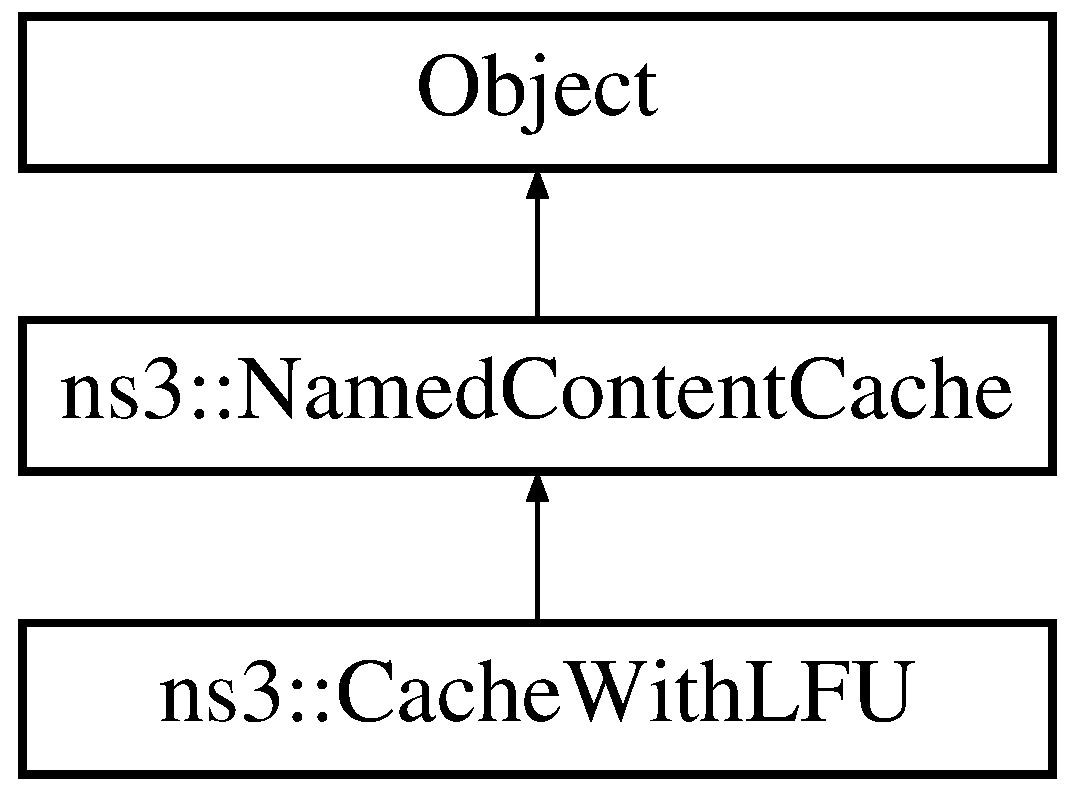
\includegraphics[height=3.000000cm]{classns3_1_1CacheWithLFU}
\end{center}
\end{figure}
\subsection*{Public Member Functions}
\begin{DoxyCompactItemize}
\item 
\hyperlink{classns3_1_1CacheWithLFU_ac9d8c2b3be42315700e643d8f2a05ffe}{Cache\-With\-L\-F\-U} ()
\item 
virtual \hyperlink{classns3_1_1CacheWithLFU_af21e5631c7e1541f819162510d093a04}{$\sim$\-Cache\-With\-L\-F\-U} ()
\item 
virtual void \hyperlink{classns3_1_1CacheWithLFU_a80bda10cdbc2edca79e6efe8e4fac60e}{Set\-Cache\-Size} (uint32\-\_\-t size)
\begin{DoxyCompactList}\small\item\em Set the cache size of the Cache. \end{DoxyCompactList}\item 
virtual uint32\-\_\-t \hyperlink{classns3_1_1CacheWithLFU_a2d58ee7990ca6ecf0db3fea70bdc09ef}{Get\-Cache\-Size} (void)
\begin{DoxyCompactList}\small\item\em Get the cache size of the Cache. \end{DoxyCompactList}\item 
virtual void \hyperlink{classns3_1_1CacheWithLFU_a3f5fc35d85cee3f4b405ccabd977662b}{Set\-Freshness\-Time} (uint64\-\_\-t time)
\begin{DoxyCompactList}\small\item\em Set the freshness time for the contents of Cache. \end{DoxyCompactList}\item 
virtual uint64\-\_\-t \hyperlink{classns3_1_1CacheWithLFU_a27a3e1d0b4b308a51ccf58dce5df9bee}{Get\-Freshness\-Time} (void)
\begin{DoxyCompactList}\small\item\em Get the freshness time set for the contents of Cache. \end{DoxyCompactList}\item 
virtual \hyperlink{classns3_1_1NamedContentCacheEntry}{Named\-Content\-Cache\-Entry} \hyperlink{classns3_1_1CacheWithLFU_a214a07a5f2af6c8532ee1a729d252f68}{Create\-Entry} (std\-::string Name, Ptr$<$ Packet $>$ packet, Ipv4\-Header ipheader)
\begin{DoxyCompactList}\small\item\em Create the Cache entry, which is an object of \hyperlink{classns3_1_1NamedContentCacheEntry}{Named\-Content\-Cache\-Entry} class. The subclasses will define this function to create an entry that has the requisite parameters of the content, for the purpose of indexing content according to caching policy the subclass represents. \end{DoxyCompactList}\item 
virtual uint32\-\_\-t \hyperlink{classns3_1_1CacheWithLFU_a8c1c53863063d36a20aab3e643301119}{Create\-Index} (\hyperlink{classns3_1_1NamedContentCacheEntry}{Named\-Content\-Cache\-Entry} entry)
\begin{DoxyCompactList}\small\item\em Create the index of the corresponding entry, by using the parameters of the content present in the entry class. The subclasses will define this function to create an index which, when put in order, will arrange the contents according to the caching policy the subclass represents. If some subclasses need decimal indexes, they have to multiply the obtained index with a factor to ensure unique integer indexes are obtained. \end{DoxyCompactList}\item 
virtual void \hyperlink{classns3_1_1CacheWithLFU_a85d1afb801554e39390c07d07d33d5e7}{Insert\-To\-Cache} (std\-::string Name, \hyperlink{classns3_1_1NamedContentCacheEntry}{Named\-Content\-Cache\-Entry} entry)
\begin{DoxyCompactList}\small\item\em Insert the Name of the content and its corresponding entry object to the Cache. \end{DoxyCompactList}\item 
virtual void \hyperlink{classns3_1_1CacheWithLFU_a5741df65535e31319d6d534ff1f8aa2f}{Insert\-To\-Policy\-Index} (uint32\-\_\-t index, std\-::string Name)
\begin{DoxyCompactList}\small\item\em Insert the index of the content and its corresponding name to the Policy\-Index. \end{DoxyCompactList}\item 
virtual bool \hyperlink{classns3_1_1CacheWithLFU_a791ed7f4bebc707e18852e346f536bd8}{Is\-Full} (void)
\begin{DoxyCompactList}\small\item\em Check if the Cache is full, i.\-e. if the number of contents is equal the cache size. \end{DoxyCompactList}\item 
virtual bool \hyperlink{classns3_1_1CacheWithLFU_a4999cd730f44907c1fdf3f8ea11f4de1}{Is\-Unique} (std\-::string Name)
\begin{DoxyCompactList}\small\item\em it check whether content is present in the cache or not \end{DoxyCompactList}\item 
virtual bool \hyperlink{classns3_1_1CacheWithLFU_a4ac9bfbe6e1b12952c345051517b762f}{Is\-Evictable} (uint32\-\_\-t index)
\begin{DoxyCompactList}\small\item\em Check if the content with the given index can be inserted with the eviction of some other content when the is full. The new content can be inserted if its index is lesser than (or greater than, when arranged in descending order) the first content, or if any content's freshness has expired. Some caching policies, like F\-I\-F\-O, keep on inserting new content, irrespective of its index. Subclasses representing such policies need not define and use this function. \end{DoxyCompactList}\item 
virtual std\-::string \hyperlink{classns3_1_1CacheWithLFU_a9dda5e2a61f82f7eaa2121a2de2f5a8f}{Evict\-Entry} (void)
\begin{DoxyCompactList}\small\item\em Evict the first content in Policy\-Index and also the corresponding entry in the Cache. This is the main eviction function of \hyperlink{classns3_1_1NamedContentCache}{Named\-Content\-Cache}. \end{DoxyCompactList}\item 
virtual void \hyperlink{classns3_1_1CacheWithLFU_aa04d4be1c2ea84020f5eac561a8ebe22}{Evict\-Entry} (std\-::string Name)
\begin{DoxyCompactList}\small\item\em Evict the content with corresponding name from both Policy\-Index and Cache. This has to be done when a packet having a content that already exists in the Cache has been received the I\-C\-N Router. This operation basically evicts the older entry of the same content so that the newer entry can be inserted. This function has to be defined by all subclasses because every content name in Cache and Policy\-Index has to be unique. \end{DoxyCompactList}\item 
virtual Ptr$<$ Packet $>$ \hyperlink{classns3_1_1CacheWithLFU_af36841e8b113ed62ad8827785fa03740}{Find} (std\-::string Name)
\begin{DoxyCompactList}\small\item\em Find the content with given name in the Cache. \end{DoxyCompactList}\item 
virtual void \hyperlink{classns3_1_1CacheWithLFU_a3b6b99b7a3c9a1e8d7fb2c5b2946f69c}{Update\-Index} (std\-::string Name)
\begin{DoxyCompactList}\small\item\em Update the index of the content with the given name. This has to be done when the content is retrieved from Cache to be sent to a querying O\-I\-C\-N Client. The subclasses will define this function based on the requirements of the caching policies they represent. \end{DoxyCompactList}\end{DoxyCompactItemize}
\subsection*{Static Public Member Functions}
\begin{DoxyCompactItemize}
\item 
static Type\-Id \hyperlink{classns3_1_1CacheWithLFU_abdbb868fedff87f723423726c8f52d18}{Get\-Type\-Id} (void)
\begin{DoxyCompactList}\small\item\em Get the type I\-D. \end{DoxyCompactList}\end{DoxyCompactItemize}
\subsection*{Private Attributes}
\begin{DoxyCompactItemize}
\item 
uint32\-\_\-t \hyperlink{classns3_1_1CacheWithLFU_a79d5772bfd23f574af448f95c223417c}{cache\-\_\-size}
\begin{DoxyCompactList}\small\item\em size of the Cache \end{DoxyCompactList}\item 
\hyperlink{classns3_1_1NamedContentCache_a9aa35d883b9f4153d97b6e7dc74f9307}{Cache} \hyperlink{classns3_1_1CacheWithLFU_a8ab1e97d5de9b643e4b29f80e971294b}{cache}
\begin{DoxyCompactList}\small\item\em main cache container which stores the name and corresponding content \end{DoxyCompactList}\item 
\hyperlink{classns3_1_1NamedContentCache_a0b728ea2d4e0acbe431897b2374cfc8e}{Policy\-Index} \hyperlink{classns3_1_1CacheWithLFU_ae17cdaaa0686b2fd2171d98ad767eec5}{policyindex}
\begin{DoxyCompactList}\small\item\em policy indexed container, containing index and content name \end{DoxyCompactList}\item 
uint64\-\_\-t \hyperlink{classns3_1_1CacheWithLFU_a8301a27e2e133723a181782ed791c3b0}{freshness\-\_\-time}
\begin{DoxyCompactList}\small\item\em time after which the cache should be evicted \end{DoxyCompactList}\end{DoxyCompactItemize}
\subsection*{Additional Inherited Members}


\subsection{Detailed Description}
This class implements the Least Frequently Used caching policy. 

\subsection{Constructor \& Destructor Documentation}
\hypertarget{classns3_1_1CacheWithLFU_ac9d8c2b3be42315700e643d8f2a05ffe}{\index{ns3\-::\-Cache\-With\-L\-F\-U@{ns3\-::\-Cache\-With\-L\-F\-U}!Cache\-With\-L\-F\-U@{Cache\-With\-L\-F\-U}}
\index{Cache\-With\-L\-F\-U@{Cache\-With\-L\-F\-U}!ns3::CacheWithLFU@{ns3\-::\-Cache\-With\-L\-F\-U}}
\subsubsection[{Cache\-With\-L\-F\-U}]{\setlength{\rightskip}{0pt plus 5cm}ns3\-::\-Cache\-With\-L\-F\-U\-::\-Cache\-With\-L\-F\-U (
\begin{DoxyParamCaption}
{}
\end{DoxyParamCaption}
)}}\label{classns3_1_1CacheWithLFU_ac9d8c2b3be42315700e643d8f2a05ffe}
\hypertarget{classns3_1_1CacheWithLFU_af21e5631c7e1541f819162510d093a04}{\index{ns3\-::\-Cache\-With\-L\-F\-U@{ns3\-::\-Cache\-With\-L\-F\-U}!$\sim$\-Cache\-With\-L\-F\-U@{$\sim$\-Cache\-With\-L\-F\-U}}
\index{$\sim$\-Cache\-With\-L\-F\-U@{$\sim$\-Cache\-With\-L\-F\-U}!ns3::CacheWithLFU@{ns3\-::\-Cache\-With\-L\-F\-U}}
\subsubsection[{$\sim$\-Cache\-With\-L\-F\-U}]{\setlength{\rightskip}{0pt plus 5cm}ns3\-::\-Cache\-With\-L\-F\-U\-::$\sim$\-Cache\-With\-L\-F\-U (
\begin{DoxyParamCaption}
{}
\end{DoxyParamCaption}
)\hspace{0.3cm}{\ttfamily [virtual]}}}\label{classns3_1_1CacheWithLFU_af21e5631c7e1541f819162510d093a04}


\subsection{Member Function Documentation}
\hypertarget{classns3_1_1CacheWithLFU_a214a07a5f2af6c8532ee1a729d252f68}{\index{ns3\-::\-Cache\-With\-L\-F\-U@{ns3\-::\-Cache\-With\-L\-F\-U}!Create\-Entry@{Create\-Entry}}
\index{Create\-Entry@{Create\-Entry}!ns3::CacheWithLFU@{ns3\-::\-Cache\-With\-L\-F\-U}}
\subsubsection[{Create\-Entry}]{\setlength{\rightskip}{0pt plus 5cm}{\bf Named\-Content\-Cache\-Entry} ns3\-::\-Cache\-With\-L\-F\-U\-::\-Create\-Entry (
\begin{DoxyParamCaption}
\item[{std\-::string}]{Name, }
\item[{Ptr$<$ Packet $>$}]{packet, }
\item[{Ipv4\-Header}]{ipheader}
\end{DoxyParamCaption}
)\hspace{0.3cm}{\ttfamily [virtual]}}}\label{classns3_1_1CacheWithLFU_a214a07a5f2af6c8532ee1a729d252f68}


Create the Cache entry, which is an object of \hyperlink{classns3_1_1NamedContentCacheEntry}{Named\-Content\-Cache\-Entry} class. The subclasses will define this function to create an entry that has the requisite parameters of the content, for the purpose of indexing content according to caching policy the subclass represents. 


\begin{DoxyParams}{Parameters}
{\em Name} & name of the content \\
\hline
{\em packet} & packet received by I\-C\-N Router, with its I\-P, Transport and O\-I\-C\-N headers removed \\
\hline
{\em ipheader} & ip header of the packet, from which the required parameters of the content (present in packet) can retrieved. \\
\hline
\end{DoxyParams}
\begin{DoxyReturn}{Returns}
the newly created cache entry 
\end{DoxyReturn}


Implements \hyperlink{classns3_1_1NamedContentCache_a154317526b3883db729c365ab342074a}{ns3\-::\-Named\-Content\-Cache}.

\hypertarget{classns3_1_1CacheWithLFU_a8c1c53863063d36a20aab3e643301119}{\index{ns3\-::\-Cache\-With\-L\-F\-U@{ns3\-::\-Cache\-With\-L\-F\-U}!Create\-Index@{Create\-Index}}
\index{Create\-Index@{Create\-Index}!ns3::CacheWithLFU@{ns3\-::\-Cache\-With\-L\-F\-U}}
\subsubsection[{Create\-Index}]{\setlength{\rightskip}{0pt plus 5cm}uint32\-\_\-t ns3\-::\-Cache\-With\-L\-F\-U\-::\-Create\-Index (
\begin{DoxyParamCaption}
\item[{{\bf Named\-Content\-Cache\-Entry}}]{entry}
\end{DoxyParamCaption}
)\hspace{0.3cm}{\ttfamily [virtual]}}}\label{classns3_1_1CacheWithLFU_a8c1c53863063d36a20aab3e643301119}


Create the index of the corresponding entry, by using the parameters of the content present in the entry class. The subclasses will define this function to create an index which, when put in order, will arrange the contents according to the caching policy the subclass represents. If some subclasses need decimal indexes, they have to multiply the obtained index with a factor to ensure unique integer indexes are obtained. 


\begin{DoxyParams}{Parameters}
{\em entry} & the cache entry corresponding to the content \\
\hline
\end{DoxyParams}
\begin{DoxyReturn}{Returns}
the newly created integer index for the content 
\end{DoxyReturn}


Implements \hyperlink{classns3_1_1NamedContentCache_a75be49c2ad5db93bdf8aaed813dcf304}{ns3\-::\-Named\-Content\-Cache}.

\hypertarget{classns3_1_1CacheWithLFU_a9dda5e2a61f82f7eaa2121a2de2f5a8f}{\index{ns3\-::\-Cache\-With\-L\-F\-U@{ns3\-::\-Cache\-With\-L\-F\-U}!Evict\-Entry@{Evict\-Entry}}
\index{Evict\-Entry@{Evict\-Entry}!ns3::CacheWithLFU@{ns3\-::\-Cache\-With\-L\-F\-U}}
\subsubsection[{Evict\-Entry}]{\setlength{\rightskip}{0pt plus 5cm}std\-::string ns3\-::\-Cache\-With\-L\-F\-U\-::\-Evict\-Entry (
\begin{DoxyParamCaption}
\item[{void}]{}
\end{DoxyParamCaption}
)\hspace{0.3cm}{\ttfamily [virtual]}}}\label{classns3_1_1CacheWithLFU_a9dda5e2a61f82f7eaa2121a2de2f5a8f}


Evict the first content in Policy\-Index and also the corresponding entry in the Cache. This is the main eviction function of \hyperlink{classns3_1_1NamedContentCache}{Named\-Content\-Cache}. 

\begin{DoxyReturn}{Returns}
the name of the evicted content 
\end{DoxyReturn}


Implements \hyperlink{classns3_1_1NamedContentCache_a87850f01fc632ede64af75d7c20f7a7e}{ns3\-::\-Named\-Content\-Cache}.

\hypertarget{classns3_1_1CacheWithLFU_aa04d4be1c2ea84020f5eac561a8ebe22}{\index{ns3\-::\-Cache\-With\-L\-F\-U@{ns3\-::\-Cache\-With\-L\-F\-U}!Evict\-Entry@{Evict\-Entry}}
\index{Evict\-Entry@{Evict\-Entry}!ns3::CacheWithLFU@{ns3\-::\-Cache\-With\-L\-F\-U}}
\subsubsection[{Evict\-Entry}]{\setlength{\rightskip}{0pt plus 5cm}void ns3\-::\-Cache\-With\-L\-F\-U\-::\-Evict\-Entry (
\begin{DoxyParamCaption}
\item[{std\-::string}]{Name}
\end{DoxyParamCaption}
)\hspace{0.3cm}{\ttfamily [virtual]}}}\label{classns3_1_1CacheWithLFU_aa04d4be1c2ea84020f5eac561a8ebe22}


Evict the content with corresponding name from both Policy\-Index and Cache. This has to be done when a packet having a content that already exists in the Cache has been received the I\-C\-N Router. This operation basically evicts the older entry of the same content so that the newer entry can be inserted. This function has to be defined by all subclasses because every content name in Cache and Policy\-Index has to be unique. 


\begin{DoxyParams}{Parameters}
{\em name} & name of the non-\/unique content \\
\hline
\end{DoxyParams}


Implements \hyperlink{classns3_1_1NamedContentCache_a254f3c74475e104a615739fc7577296f}{ns3\-::\-Named\-Content\-Cache}.

\hypertarget{classns3_1_1CacheWithLFU_af36841e8b113ed62ad8827785fa03740}{\index{ns3\-::\-Cache\-With\-L\-F\-U@{ns3\-::\-Cache\-With\-L\-F\-U}!Find@{Find}}
\index{Find@{Find}!ns3::CacheWithLFU@{ns3\-::\-Cache\-With\-L\-F\-U}}
\subsubsection[{Find}]{\setlength{\rightskip}{0pt plus 5cm}Ptr$<$ Packet $>$ ns3\-::\-Cache\-With\-L\-F\-U\-::\-Find (
\begin{DoxyParamCaption}
\item[{std\-::string}]{Name}
\end{DoxyParamCaption}
)\hspace{0.3cm}{\ttfamily [virtual]}}}\label{classns3_1_1CacheWithLFU_af36841e8b113ed62ad8827785fa03740}


Find the content with given name in the Cache. 

\begin{DoxyReturn}{Returns}
the content in the form of an Application Layer packet 
\end{DoxyReturn}


Implements \hyperlink{classns3_1_1NamedContentCache_a081439cd96d09e2f9f158f3aebe9fd7c}{ns3\-::\-Named\-Content\-Cache}.

\hypertarget{classns3_1_1CacheWithLFU_a2d58ee7990ca6ecf0db3fea70bdc09ef}{\index{ns3\-::\-Cache\-With\-L\-F\-U@{ns3\-::\-Cache\-With\-L\-F\-U}!Get\-Cache\-Size@{Get\-Cache\-Size}}
\index{Get\-Cache\-Size@{Get\-Cache\-Size}!ns3::CacheWithLFU@{ns3\-::\-Cache\-With\-L\-F\-U}}
\subsubsection[{Get\-Cache\-Size}]{\setlength{\rightskip}{0pt plus 5cm}uint32\-\_\-t ns3\-::\-Cache\-With\-L\-F\-U\-::\-Get\-Cache\-Size (
\begin{DoxyParamCaption}
\item[{void}]{}
\end{DoxyParamCaption}
)\hspace{0.3cm}{\ttfamily [virtual]}}}\label{classns3_1_1CacheWithLFU_a2d58ee7990ca6ecf0db3fea70bdc09ef}


Get the cache size of the Cache. 

\begin{DoxyReturn}{Returns}
the cache size of the Cache 
\end{DoxyReturn}


Implements \hyperlink{classns3_1_1NamedContentCache_afd9ade17d87082a46cbb745fd0196ab4}{ns3\-::\-Named\-Content\-Cache}.

\hypertarget{classns3_1_1CacheWithLFU_a27a3e1d0b4b308a51ccf58dce5df9bee}{\index{ns3\-::\-Cache\-With\-L\-F\-U@{ns3\-::\-Cache\-With\-L\-F\-U}!Get\-Freshness\-Time@{Get\-Freshness\-Time}}
\index{Get\-Freshness\-Time@{Get\-Freshness\-Time}!ns3::CacheWithLFU@{ns3\-::\-Cache\-With\-L\-F\-U}}
\subsubsection[{Get\-Freshness\-Time}]{\setlength{\rightskip}{0pt plus 5cm}uint64\-\_\-t ns3\-::\-Cache\-With\-L\-F\-U\-::\-Get\-Freshness\-Time (
\begin{DoxyParamCaption}
\item[{void}]{}
\end{DoxyParamCaption}
)\hspace{0.3cm}{\ttfamily [virtual]}}}\label{classns3_1_1CacheWithLFU_a27a3e1d0b4b308a51ccf58dce5df9bee}


Get the freshness time set for the contents of Cache. 

\begin{DoxyReturn}{Returns}
the freshness time in milliseconds 
\end{DoxyReturn}


Implements \hyperlink{classns3_1_1NamedContentCache_ac2b0e616d4e866cb2328e986f2ef69e1}{ns3\-::\-Named\-Content\-Cache}.

\hypertarget{classns3_1_1CacheWithLFU_abdbb868fedff87f723423726c8f52d18}{\index{ns3\-::\-Cache\-With\-L\-F\-U@{ns3\-::\-Cache\-With\-L\-F\-U}!Get\-Type\-Id@{Get\-Type\-Id}}
\index{Get\-Type\-Id@{Get\-Type\-Id}!ns3::CacheWithLFU@{ns3\-::\-Cache\-With\-L\-F\-U}}
\subsubsection[{Get\-Type\-Id}]{\setlength{\rightskip}{0pt plus 5cm}Type\-Id ns3\-::\-Cache\-With\-L\-F\-U\-::\-Get\-Type\-Id (
\begin{DoxyParamCaption}
\item[{void}]{}
\end{DoxyParamCaption}
)\hspace{0.3cm}{\ttfamily [static]}}}\label{classns3_1_1CacheWithLFU_abdbb868fedff87f723423726c8f52d18}


Get the type I\-D. 

\begin{DoxyReturn}{Returns}
the object Type\-Id 
\end{DoxyReturn}
\hypertarget{classns3_1_1CacheWithLFU_a85d1afb801554e39390c07d07d33d5e7}{\index{ns3\-::\-Cache\-With\-L\-F\-U@{ns3\-::\-Cache\-With\-L\-F\-U}!Insert\-To\-Cache@{Insert\-To\-Cache}}
\index{Insert\-To\-Cache@{Insert\-To\-Cache}!ns3::CacheWithLFU@{ns3\-::\-Cache\-With\-L\-F\-U}}
\subsubsection[{Insert\-To\-Cache}]{\setlength{\rightskip}{0pt plus 5cm}void ns3\-::\-Cache\-With\-L\-F\-U\-::\-Insert\-To\-Cache (
\begin{DoxyParamCaption}
\item[{std\-::string}]{Name, }
\item[{{\bf Named\-Content\-Cache\-Entry}}]{entry}
\end{DoxyParamCaption}
)\hspace{0.3cm}{\ttfamily [virtual]}}}\label{classns3_1_1CacheWithLFU_a85d1afb801554e39390c07d07d33d5e7}


Insert the Name of the content and its corresponding entry object to the Cache. 


\begin{DoxyParams}{Parameters}
{\em Name} & name of the content \\
\hline
{\em entry} & the cache entry corresponding to the content \\
\hline
\end{DoxyParams}


Implements \hyperlink{classns3_1_1NamedContentCache_a56a23add9b5bc03908793cf261ccb5f8}{ns3\-::\-Named\-Content\-Cache}.

\hypertarget{classns3_1_1CacheWithLFU_a5741df65535e31319d6d534ff1f8aa2f}{\index{ns3\-::\-Cache\-With\-L\-F\-U@{ns3\-::\-Cache\-With\-L\-F\-U}!Insert\-To\-Policy\-Index@{Insert\-To\-Policy\-Index}}
\index{Insert\-To\-Policy\-Index@{Insert\-To\-Policy\-Index}!ns3::CacheWithLFU@{ns3\-::\-Cache\-With\-L\-F\-U}}
\subsubsection[{Insert\-To\-Policy\-Index}]{\setlength{\rightskip}{0pt plus 5cm}void ns3\-::\-Cache\-With\-L\-F\-U\-::\-Insert\-To\-Policy\-Index (
\begin{DoxyParamCaption}
\item[{uint32\-\_\-t}]{index, }
\item[{std\-::string}]{Name}
\end{DoxyParamCaption}
)\hspace{0.3cm}{\ttfamily [virtual]}}}\label{classns3_1_1CacheWithLFU_a5741df65535e31319d6d534ff1f8aa2f}


Insert the index of the content and its corresponding name to the Policy\-Index. 


\begin{DoxyParams}{Parameters}
{\em index} & the unique integer index of the content \\
\hline
{\em Name} & name of the content \\
\hline
\end{DoxyParams}


Implements \hyperlink{classns3_1_1NamedContentCache_ac248e647f56a6fef10285b1c654b8180}{ns3\-::\-Named\-Content\-Cache}.

\hypertarget{classns3_1_1CacheWithLFU_a4ac9bfbe6e1b12952c345051517b762f}{\index{ns3\-::\-Cache\-With\-L\-F\-U@{ns3\-::\-Cache\-With\-L\-F\-U}!Is\-Evictable@{Is\-Evictable}}
\index{Is\-Evictable@{Is\-Evictable}!ns3::CacheWithLFU@{ns3\-::\-Cache\-With\-L\-F\-U}}
\subsubsection[{Is\-Evictable}]{\setlength{\rightskip}{0pt plus 5cm}bool ns3\-::\-Cache\-With\-L\-F\-U\-::\-Is\-Evictable (
\begin{DoxyParamCaption}
\item[{uint32\-\_\-t}]{index}
\end{DoxyParamCaption}
)\hspace{0.3cm}{\ttfamily [virtual]}}}\label{classns3_1_1CacheWithLFU_a4ac9bfbe6e1b12952c345051517b762f}


Check if the content with the given index can be inserted with the eviction of some other content when the is full. The new content can be inserted if its index is lesser than (or greater than, when arranged in descending order) the first content, or if any content's freshness has expired. Some caching policies, like F\-I\-F\-O, keep on inserting new content, irrespective of its index. Subclasses representing such policies need not define and use this function. 


\begin{DoxyParams}{Parameters}
{\em index} & the unique integer index of the content \\
\hline
\end{DoxyParams}
\begin{DoxyReturn}{Returns}
true if any existing content can be evicted so that the new content with the given index can be inserted. 
\end{DoxyReturn}


Implements \hyperlink{classns3_1_1NamedContentCache_a281ad340f9771fa2ed898a1ad569d0da}{ns3\-::\-Named\-Content\-Cache}.

\hypertarget{classns3_1_1CacheWithLFU_a791ed7f4bebc707e18852e346f536bd8}{\index{ns3\-::\-Cache\-With\-L\-F\-U@{ns3\-::\-Cache\-With\-L\-F\-U}!Is\-Full@{Is\-Full}}
\index{Is\-Full@{Is\-Full}!ns3::CacheWithLFU@{ns3\-::\-Cache\-With\-L\-F\-U}}
\subsubsection[{Is\-Full}]{\setlength{\rightskip}{0pt plus 5cm}bool ns3\-::\-Cache\-With\-L\-F\-U\-::\-Is\-Full (
\begin{DoxyParamCaption}
\item[{void}]{}
\end{DoxyParamCaption}
)\hspace{0.3cm}{\ttfamily [virtual]}}}\label{classns3_1_1CacheWithLFU_a791ed7f4bebc707e18852e346f536bd8}


Check if the Cache is full, i.\-e. if the number of contents is equal the cache size. 

\begin{DoxyReturn}{Returns}
true if the Cache is full 
\end{DoxyReturn}


Implements \hyperlink{classns3_1_1NamedContentCache_a1ceeaf5b85d3571225adfe2d48caf126}{ns3\-::\-Named\-Content\-Cache}.

\hypertarget{classns3_1_1CacheWithLFU_a4999cd730f44907c1fdf3f8ea11f4de1}{\index{ns3\-::\-Cache\-With\-L\-F\-U@{ns3\-::\-Cache\-With\-L\-F\-U}!Is\-Unique@{Is\-Unique}}
\index{Is\-Unique@{Is\-Unique}!ns3::CacheWithLFU@{ns3\-::\-Cache\-With\-L\-F\-U}}
\subsubsection[{Is\-Unique}]{\setlength{\rightskip}{0pt plus 5cm}bool ns3\-::\-Cache\-With\-L\-F\-U\-::\-Is\-Unique (
\begin{DoxyParamCaption}
\item[{std\-::string}]{name}
\end{DoxyParamCaption}
)\hspace{0.3cm}{\ttfamily [virtual]}}}\label{classns3_1_1CacheWithLFU_a4999cd730f44907c1fdf3f8ea11f4de1}


it check whether content is present in the cache or not 


\begin{DoxyParams}{Parameters}
{\em name} & name of the content \\
\hline
\end{DoxyParams}
\begin{DoxyReturn}{Returns}
true if content is not present, false when content is present in the cache 
\end{DoxyReturn}


Implements \hyperlink{classns3_1_1NamedContentCache_a4c4a79310c99f9c8ad6227d3b380dc20}{ns3\-::\-Named\-Content\-Cache}.

\hypertarget{classns3_1_1CacheWithLFU_a80bda10cdbc2edca79e6efe8e4fac60e}{\index{ns3\-::\-Cache\-With\-L\-F\-U@{ns3\-::\-Cache\-With\-L\-F\-U}!Set\-Cache\-Size@{Set\-Cache\-Size}}
\index{Set\-Cache\-Size@{Set\-Cache\-Size}!ns3::CacheWithLFU@{ns3\-::\-Cache\-With\-L\-F\-U}}
\subsubsection[{Set\-Cache\-Size}]{\setlength{\rightskip}{0pt plus 5cm}void ns3\-::\-Cache\-With\-L\-F\-U\-::\-Set\-Cache\-Size (
\begin{DoxyParamCaption}
\item[{uint32\-\_\-t}]{size}
\end{DoxyParamCaption}
)\hspace{0.3cm}{\ttfamily [virtual]}}}\label{classns3_1_1CacheWithLFU_a80bda10cdbc2edca79e6efe8e4fac60e}


Set the cache size of the Cache. 


\begin{DoxyParams}{Parameters}
{\em size} & the size to which the cache has to be set \\
\hline
\end{DoxyParams}


Implements \hyperlink{classns3_1_1NamedContentCache_ae28605a03a5a4d8b9a3494b4068f44e2}{ns3\-::\-Named\-Content\-Cache}.

\hypertarget{classns3_1_1CacheWithLFU_a3f5fc35d85cee3f4b405ccabd977662b}{\index{ns3\-::\-Cache\-With\-L\-F\-U@{ns3\-::\-Cache\-With\-L\-F\-U}!Set\-Freshness\-Time@{Set\-Freshness\-Time}}
\index{Set\-Freshness\-Time@{Set\-Freshness\-Time}!ns3::CacheWithLFU@{ns3\-::\-Cache\-With\-L\-F\-U}}
\subsubsection[{Set\-Freshness\-Time}]{\setlength{\rightskip}{0pt plus 5cm}void ns3\-::\-Cache\-With\-L\-F\-U\-::\-Set\-Freshness\-Time (
\begin{DoxyParamCaption}
\item[{uint64\-\_\-t}]{time}
\end{DoxyParamCaption}
)\hspace{0.3cm}{\ttfamily [virtual]}}}\label{classns3_1_1CacheWithLFU_a3f5fc35d85cee3f4b405ccabd977662b}


Set the freshness time for the contents of Cache. 


\begin{DoxyParams}{Parameters}
{\em time} & the freshness time in milliseconds \\
\hline
\end{DoxyParams}


Implements \hyperlink{classns3_1_1NamedContentCache_a92a5e2e641a11d15300f621aa77275ab}{ns3\-::\-Named\-Content\-Cache}.

\hypertarget{classns3_1_1CacheWithLFU_a3b6b99b7a3c9a1e8d7fb2c5b2946f69c}{\index{ns3\-::\-Cache\-With\-L\-F\-U@{ns3\-::\-Cache\-With\-L\-F\-U}!Update\-Index@{Update\-Index}}
\index{Update\-Index@{Update\-Index}!ns3::CacheWithLFU@{ns3\-::\-Cache\-With\-L\-F\-U}}
\subsubsection[{Update\-Index}]{\setlength{\rightskip}{0pt plus 5cm}void ns3\-::\-Cache\-With\-L\-F\-U\-::\-Update\-Index (
\begin{DoxyParamCaption}
\item[{std\-::string}]{Name}
\end{DoxyParamCaption}
)\hspace{0.3cm}{\ttfamily [virtual]}}}\label{classns3_1_1CacheWithLFU_a3b6b99b7a3c9a1e8d7fb2c5b2946f69c}


Update the index of the content with the given name. This has to be done when the content is retrieved from Cache to be sent to a querying O\-I\-C\-N Client. The subclasses will define this function based on the requirements of the caching policies they represent. 


\begin{DoxyParams}{Parameters}
{\em the} & name of the content whose index has to be updated \\
\hline
\end{DoxyParams}


Implements \hyperlink{classns3_1_1NamedContentCache_aeabf8afacd89cbc46b78b382c8a487e8}{ns3\-::\-Named\-Content\-Cache}.



\subsection{Member Data Documentation}
\hypertarget{classns3_1_1CacheWithLFU_a8ab1e97d5de9b643e4b29f80e971294b}{\index{ns3\-::\-Cache\-With\-L\-F\-U@{ns3\-::\-Cache\-With\-L\-F\-U}!cache@{cache}}
\index{cache@{cache}!ns3::CacheWithLFU@{ns3\-::\-Cache\-With\-L\-F\-U}}
\subsubsection[{cache}]{\setlength{\rightskip}{0pt plus 5cm}{\bf Cache} ns3\-::\-Cache\-With\-L\-F\-U\-::cache\hspace{0.3cm}{\ttfamily [private]}}}\label{classns3_1_1CacheWithLFU_a8ab1e97d5de9b643e4b29f80e971294b}


main cache container which stores the name and corresponding content 

\hypertarget{classns3_1_1CacheWithLFU_a79d5772bfd23f574af448f95c223417c}{\index{ns3\-::\-Cache\-With\-L\-F\-U@{ns3\-::\-Cache\-With\-L\-F\-U}!cache\-\_\-size@{cache\-\_\-size}}
\index{cache\-\_\-size@{cache\-\_\-size}!ns3::CacheWithLFU@{ns3\-::\-Cache\-With\-L\-F\-U}}
\subsubsection[{cache\-\_\-size}]{\setlength{\rightskip}{0pt plus 5cm}uint32\-\_\-t ns3\-::\-Cache\-With\-L\-F\-U\-::cache\-\_\-size\hspace{0.3cm}{\ttfamily [private]}}}\label{classns3_1_1CacheWithLFU_a79d5772bfd23f574af448f95c223417c}


size of the Cache 

\hypertarget{classns3_1_1CacheWithLFU_a8301a27e2e133723a181782ed791c3b0}{\index{ns3\-::\-Cache\-With\-L\-F\-U@{ns3\-::\-Cache\-With\-L\-F\-U}!freshness\-\_\-time@{freshness\-\_\-time}}
\index{freshness\-\_\-time@{freshness\-\_\-time}!ns3::CacheWithLFU@{ns3\-::\-Cache\-With\-L\-F\-U}}
\subsubsection[{freshness\-\_\-time}]{\setlength{\rightskip}{0pt plus 5cm}uint64\-\_\-t ns3\-::\-Cache\-With\-L\-F\-U\-::freshness\-\_\-time\hspace{0.3cm}{\ttfamily [private]}}}\label{classns3_1_1CacheWithLFU_a8301a27e2e133723a181782ed791c3b0}


time after which the cache should be evicted 

\hypertarget{classns3_1_1CacheWithLFU_ae17cdaaa0686b2fd2171d98ad767eec5}{\index{ns3\-::\-Cache\-With\-L\-F\-U@{ns3\-::\-Cache\-With\-L\-F\-U}!policyindex@{policyindex}}
\index{policyindex@{policyindex}!ns3::CacheWithLFU@{ns3\-::\-Cache\-With\-L\-F\-U}}
\subsubsection[{policyindex}]{\setlength{\rightskip}{0pt plus 5cm}{\bf Policy\-Index} ns3\-::\-Cache\-With\-L\-F\-U\-::policyindex\hspace{0.3cm}{\ttfamily [private]}}}\label{classns3_1_1CacheWithLFU_ae17cdaaa0686b2fd2171d98ad767eec5}


policy indexed container, containing index and content name 



The documentation for this class was generated from the following files\-:\begin{DoxyCompactItemize}
\item 
model/\hyperlink{cache-with-lfu_8h}{cache-\/with-\/lfu.\-h}\item 
model/\hyperlink{cache-with-lfu_8cc}{cache-\/with-\/lfu.\-cc}\end{DoxyCompactItemize}

\hypertarget{classns3_1_1CacheWithLRU}{\section{ns3\-:\-:Cache\-With\-L\-R\-U Class Reference}
\label{classns3_1_1CacheWithLRU}\index{ns3\-::\-Cache\-With\-L\-R\-U@{ns3\-::\-Cache\-With\-L\-R\-U}}
}


This class implements the Least Recently Used caching policy.  




{\ttfamily \#include $<$cache-\/with-\/lru.\-h$>$}

Inheritance diagram for ns3\-:\-:Cache\-With\-L\-R\-U\-:\begin{figure}[H]
\begin{center}
\leavevmode
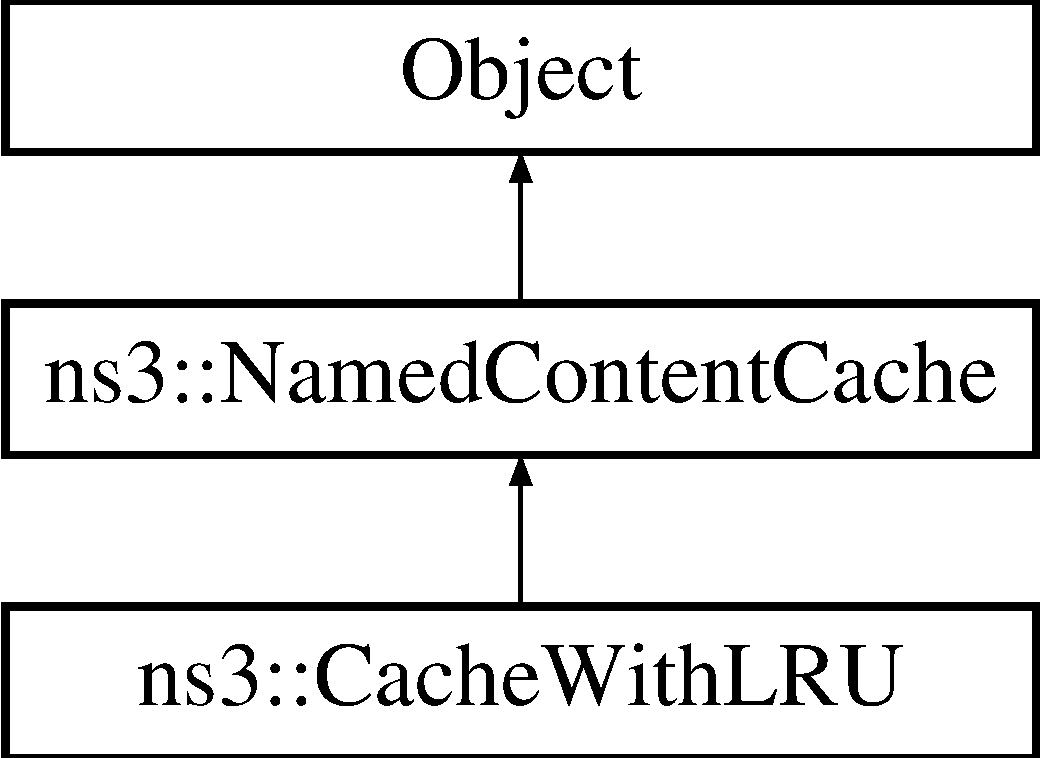
\includegraphics[height=3.000000cm]{classns3_1_1CacheWithLRU}
\end{center}
\end{figure}
\subsection*{Public Member Functions}
\begin{DoxyCompactItemize}
\item 
\hyperlink{classns3_1_1CacheWithLRU_ad16e5fd5c30972ad02742b2b60d6f108}{Cache\-With\-L\-R\-U} ()
\item 
virtual \hyperlink{classns3_1_1CacheWithLRU_a7d21d57b377db88ba971fd324194e150}{$\sim$\-Cache\-With\-L\-R\-U} ()
\item 
virtual void \hyperlink{classns3_1_1CacheWithLRU_a75323b8c1d45dbaa19e07bf6fdf9b9a3}{Set\-Cache\-Size} (uint32\-\_\-t size)
\begin{DoxyCompactList}\small\item\em Set the cache size of the Cache. \end{DoxyCompactList}\item 
virtual uint32\-\_\-t \hyperlink{classns3_1_1CacheWithLRU_a7011075202d46dc23358058ed8037125}{Get\-Cache\-Size} (void)
\begin{DoxyCompactList}\small\item\em Get the cache size of the Cache. \end{DoxyCompactList}\item 
virtual void \hyperlink{classns3_1_1CacheWithLRU_a0f9e4e62cf6dee79d05774b25ee398c5}{Set\-Freshness\-Time} (uint64\-\_\-t time)
\begin{DoxyCompactList}\small\item\em Set the freshness time for the contents of Cache. \end{DoxyCompactList}\item 
virtual uint64\-\_\-t \hyperlink{classns3_1_1CacheWithLRU_ad3f0a3b34a506792f30310761242a86c}{Get\-Freshness\-Time} (void)
\begin{DoxyCompactList}\small\item\em Get the freshness time set for the contents of Cache. \end{DoxyCompactList}\item 
virtual \hyperlink{classns3_1_1NamedContentCacheEntry}{Named\-Content\-Cache\-Entry} \hyperlink{classns3_1_1CacheWithLRU_a8dc721b8593047e5246b3ffa21c83ba2}{Create\-Entry} (std\-::string Name, Ptr$<$ Packet $>$ packet, Ipv4\-Header ipheader)
\begin{DoxyCompactList}\small\item\em Create the Cache entry, which is an object of \hyperlink{classns3_1_1NamedContentCacheEntry}{Named\-Content\-Cache\-Entry} class. The subclasses will define this function to create an entry that has the requisite parameters of the content, for the purpose of indexing content according to caching policy the subclass represents. \end{DoxyCompactList}\item 
virtual uint32\-\_\-t \hyperlink{classns3_1_1CacheWithLRU_a5129171c03d524afe292aec079397d40}{Create\-Index} (\hyperlink{classns3_1_1NamedContentCacheEntry}{Named\-Content\-Cache\-Entry} entry)
\begin{DoxyCompactList}\small\item\em Create the index of the corresponding entry, by using the parameters of the content present in the entry class. The subclasses will define this function to create an index which, when put in order, will arrange the contents according to the caching policy the subclass represents. If some subclasses need decimal indexes, they have to multiply the obtained index with a factor to ensure unique integer indexes are obtained. \end{DoxyCompactList}\item 
virtual void \hyperlink{classns3_1_1CacheWithLRU_adfce286e921a3f3d4cbf9e1008cae632}{Insert\-To\-Cache} (std\-::string Name, \hyperlink{classns3_1_1NamedContentCacheEntry}{Named\-Content\-Cache\-Entry} entry)
\begin{DoxyCompactList}\small\item\em Insert the Name of the content and its corresponding entry object to the Cache. \end{DoxyCompactList}\item 
virtual void \hyperlink{classns3_1_1CacheWithLRU_a8b5e0eb51220cba226f913ddc1ef304f}{Insert\-To\-Policy\-Index} (uint32\-\_\-t index, std\-::string Name)
\begin{DoxyCompactList}\small\item\em Insert the index of the content and its corresponding name to the Policy\-Index. \end{DoxyCompactList}\item 
virtual bool \hyperlink{classns3_1_1CacheWithLRU_ac8cea24f840cdfb15abb1f09638b0fb1}{Is\-Full} (void)
\begin{DoxyCompactList}\small\item\em Check if the Cache is full, i.\-e. if the number of contents is equal the cache size. \end{DoxyCompactList}\item 
virtual bool \hyperlink{classns3_1_1CacheWithLRU_a8c69352212c41da32499d84add8dd42d}{Is\-Unique} (std\-::string Name)
\begin{DoxyCompactList}\small\item\em it check whether content is present in the cache or not \end{DoxyCompactList}\item 
virtual bool \hyperlink{classns3_1_1CacheWithLRU_a29fae4efb96e97023459866634488a28}{Is\-Evictable} (uint32\-\_\-t index)
\begin{DoxyCompactList}\small\item\em Check if the content with the given index can be inserted with the eviction of some other content when the is full. The new content can be inserted if its index is lesser than (or greater than, when arranged in descending order) the first content, or if any content's freshness has expired. Some caching policies, like F\-I\-F\-O, keep on inserting new content, irrespective of its index. Subclasses representing such policies need not define and use this function. \end{DoxyCompactList}\item 
virtual std\-::string \hyperlink{classns3_1_1CacheWithLRU_a657627f6ab6b395086c44bf7e51063fc}{Evict\-Entry} (void)
\begin{DoxyCompactList}\small\item\em Evict the first content in Policy\-Index and also the corresponding entry in the Cache. This is the main eviction function of \hyperlink{classns3_1_1NamedContentCache}{Named\-Content\-Cache}. \end{DoxyCompactList}\item 
virtual void \hyperlink{classns3_1_1CacheWithLRU_abd2898e58b7eeb214153a29379e05404}{Evict\-Entry} (std\-::string Name)
\begin{DoxyCompactList}\small\item\em Evict the content with corresponding name from both Policy\-Index and Cache. This has to be done when a packet having a content that already exists in the Cache has been received the I\-C\-N Router. This operation basically evicts the older entry of the same content so that the newer entry can be inserted. This function has to be defined by all subclasses because every content name in Cache and Policy\-Index has to be unique. \end{DoxyCompactList}\item 
virtual Ptr$<$ Packet $>$ \hyperlink{classns3_1_1CacheWithLRU_a2948736630124fd3a5efcdc69ac04126}{Find} (std\-::string Name)
\begin{DoxyCompactList}\small\item\em Find the content with given name in the Cache. \end{DoxyCompactList}\item 
virtual void \hyperlink{classns3_1_1CacheWithLRU_ad4a24104ec617f5e4fb163a0f7416352}{Update\-Index} (std\-::string Name)
\begin{DoxyCompactList}\small\item\em Update the index of the content with the given name. This has to be done when the content is retrieved from Cache to be sent to a querying O\-I\-C\-N Client. The subclasses will define this function based on the requirements of the caching policies they represent. \end{DoxyCompactList}\end{DoxyCompactItemize}
\subsection*{Static Public Member Functions}
\begin{DoxyCompactItemize}
\item 
static Type\-Id \hyperlink{classns3_1_1CacheWithLRU_aa84deadfb0a84e5c63abe3a0f59c06d8}{Get\-Type\-Id} (void)
\end{DoxyCompactItemize}
\subsection*{Private Attributes}
\begin{DoxyCompactItemize}
\item 
uint32\-\_\-t \hyperlink{classns3_1_1CacheWithLRU_a9bd4ccdfb85587489ed2832695e0da62}{cache\-\_\-size}
\begin{DoxyCompactList}\small\item\em size of the Cache \end{DoxyCompactList}\item 
\hyperlink{classns3_1_1NamedContentCache_a9aa35d883b9f4153d97b6e7dc74f9307}{Cache} \hyperlink{classns3_1_1CacheWithLRU_ae7ffb4f0cbe5e8e6d769b71dc26d61d4}{cache}
\begin{DoxyCompactList}\small\item\em main cache container which stores the name and corresponding content \end{DoxyCompactList}\item 
\hyperlink{classns3_1_1NamedContentCache_a0b728ea2d4e0acbe431897b2374cfc8e}{Policy\-Index} \hyperlink{classns3_1_1CacheWithLRU_ada6a1db505251a0b7d96a18cf5cf0f1b}{policyindex}
\begin{DoxyCompactList}\small\item\em policy indexed container, containing index and content name \end{DoxyCompactList}\end{DoxyCompactItemize}
\subsection*{Additional Inherited Members}


\subsection{Detailed Description}
This class implements the Least Recently Used caching policy. 

\subsection{Constructor \& Destructor Documentation}
\hypertarget{classns3_1_1CacheWithLRU_ad16e5fd5c30972ad02742b2b60d6f108}{\index{ns3\-::\-Cache\-With\-L\-R\-U@{ns3\-::\-Cache\-With\-L\-R\-U}!Cache\-With\-L\-R\-U@{Cache\-With\-L\-R\-U}}
\index{Cache\-With\-L\-R\-U@{Cache\-With\-L\-R\-U}!ns3::CacheWithLRU@{ns3\-::\-Cache\-With\-L\-R\-U}}
\subsubsection[{Cache\-With\-L\-R\-U}]{\setlength{\rightskip}{0pt plus 5cm}ns3\-::\-Cache\-With\-L\-R\-U\-::\-Cache\-With\-L\-R\-U (
\begin{DoxyParamCaption}
{}
\end{DoxyParamCaption}
)}}\label{classns3_1_1CacheWithLRU_ad16e5fd5c30972ad02742b2b60d6f108}
\hypertarget{classns3_1_1CacheWithLRU_a7d21d57b377db88ba971fd324194e150}{\index{ns3\-::\-Cache\-With\-L\-R\-U@{ns3\-::\-Cache\-With\-L\-R\-U}!$\sim$\-Cache\-With\-L\-R\-U@{$\sim$\-Cache\-With\-L\-R\-U}}
\index{$\sim$\-Cache\-With\-L\-R\-U@{$\sim$\-Cache\-With\-L\-R\-U}!ns3::CacheWithLRU@{ns3\-::\-Cache\-With\-L\-R\-U}}
\subsubsection[{$\sim$\-Cache\-With\-L\-R\-U}]{\setlength{\rightskip}{0pt plus 5cm}ns3\-::\-Cache\-With\-L\-R\-U\-::$\sim$\-Cache\-With\-L\-R\-U (
\begin{DoxyParamCaption}
{}
\end{DoxyParamCaption}
)\hspace{0.3cm}{\ttfamily [virtual]}}}\label{classns3_1_1CacheWithLRU_a7d21d57b377db88ba971fd324194e150}


\subsection{Member Function Documentation}
\hypertarget{classns3_1_1CacheWithLRU_a8dc721b8593047e5246b3ffa21c83ba2}{\index{ns3\-::\-Cache\-With\-L\-R\-U@{ns3\-::\-Cache\-With\-L\-R\-U}!Create\-Entry@{Create\-Entry}}
\index{Create\-Entry@{Create\-Entry}!ns3::CacheWithLRU@{ns3\-::\-Cache\-With\-L\-R\-U}}
\subsubsection[{Create\-Entry}]{\setlength{\rightskip}{0pt plus 5cm}{\bf Named\-Content\-Cache\-Entry} ns3\-::\-Cache\-With\-L\-R\-U\-::\-Create\-Entry (
\begin{DoxyParamCaption}
\item[{std\-::string}]{Name, }
\item[{Ptr$<$ Packet $>$}]{packet, }
\item[{Ipv4\-Header}]{ipheader}
\end{DoxyParamCaption}
)\hspace{0.3cm}{\ttfamily [virtual]}}}\label{classns3_1_1CacheWithLRU_a8dc721b8593047e5246b3ffa21c83ba2}


Create the Cache entry, which is an object of \hyperlink{classns3_1_1NamedContentCacheEntry}{Named\-Content\-Cache\-Entry} class. The subclasses will define this function to create an entry that has the requisite parameters of the content, for the purpose of indexing content according to caching policy the subclass represents. 


\begin{DoxyParams}{Parameters}
{\em Name} & name of the content \\
\hline
{\em packet} & packet received by I\-C\-N Router, with its I\-P, Transport and O\-I\-C\-N headers removed \\
\hline
{\em ipheader} & I\-P Header of the packet, from which the required parameters of the content (present in packet) can retrieved. \\
\hline
\end{DoxyParams}
\begin{DoxyReturn}{Returns}
the newly created cache entry 
\end{DoxyReturn}


Implements \hyperlink{classns3_1_1NamedContentCache_a154317526b3883db729c365ab342074a}{ns3\-::\-Named\-Content\-Cache}.

\hypertarget{classns3_1_1CacheWithLRU_a5129171c03d524afe292aec079397d40}{\index{ns3\-::\-Cache\-With\-L\-R\-U@{ns3\-::\-Cache\-With\-L\-R\-U}!Create\-Index@{Create\-Index}}
\index{Create\-Index@{Create\-Index}!ns3::CacheWithLRU@{ns3\-::\-Cache\-With\-L\-R\-U}}
\subsubsection[{Create\-Index}]{\setlength{\rightskip}{0pt plus 5cm}uint32\-\_\-t ns3\-::\-Cache\-With\-L\-R\-U\-::\-Create\-Index (
\begin{DoxyParamCaption}
\item[{{\bf Named\-Content\-Cache\-Entry}}]{entry}
\end{DoxyParamCaption}
)\hspace{0.3cm}{\ttfamily [virtual]}}}\label{classns3_1_1CacheWithLRU_a5129171c03d524afe292aec079397d40}


Create the index of the corresponding entry, by using the parameters of the content present in the entry class. The subclasses will define this function to create an index which, when put in order, will arrange the contents according to the caching policy the subclass represents. If some subclasses need decimal indexes, they have to multiply the obtained index with a factor to ensure unique integer indexes are obtained. 


\begin{DoxyParams}{Parameters}
{\em entry} & the cache entry corresponding to the content \\
\hline
\end{DoxyParams}
\begin{DoxyReturn}{Returns}
the newly created integer index for the content 
\end{DoxyReturn}


Implements \hyperlink{classns3_1_1NamedContentCache_a75be49c2ad5db93bdf8aaed813dcf304}{ns3\-::\-Named\-Content\-Cache}.

\hypertarget{classns3_1_1CacheWithLRU_a657627f6ab6b395086c44bf7e51063fc}{\index{ns3\-::\-Cache\-With\-L\-R\-U@{ns3\-::\-Cache\-With\-L\-R\-U}!Evict\-Entry@{Evict\-Entry}}
\index{Evict\-Entry@{Evict\-Entry}!ns3::CacheWithLRU@{ns3\-::\-Cache\-With\-L\-R\-U}}
\subsubsection[{Evict\-Entry}]{\setlength{\rightskip}{0pt plus 5cm}std\-::string ns3\-::\-Cache\-With\-L\-R\-U\-::\-Evict\-Entry (
\begin{DoxyParamCaption}
\item[{void}]{}
\end{DoxyParamCaption}
)\hspace{0.3cm}{\ttfamily [virtual]}}}\label{classns3_1_1CacheWithLRU_a657627f6ab6b395086c44bf7e51063fc}


Evict the first content in Policy\-Index and also the corresponding entry in the Cache. This is the main eviction function of \hyperlink{classns3_1_1NamedContentCache}{Named\-Content\-Cache}. 

\begin{DoxyReturn}{Returns}
the name of the evicted content 
\end{DoxyReturn}


Implements \hyperlink{classns3_1_1NamedContentCache_a87850f01fc632ede64af75d7c20f7a7e}{ns3\-::\-Named\-Content\-Cache}.

\hypertarget{classns3_1_1CacheWithLRU_abd2898e58b7eeb214153a29379e05404}{\index{ns3\-::\-Cache\-With\-L\-R\-U@{ns3\-::\-Cache\-With\-L\-R\-U}!Evict\-Entry@{Evict\-Entry}}
\index{Evict\-Entry@{Evict\-Entry}!ns3::CacheWithLRU@{ns3\-::\-Cache\-With\-L\-R\-U}}
\subsubsection[{Evict\-Entry}]{\setlength{\rightskip}{0pt plus 5cm}void ns3\-::\-Cache\-With\-L\-R\-U\-::\-Evict\-Entry (
\begin{DoxyParamCaption}
\item[{std\-::string}]{Name}
\end{DoxyParamCaption}
)\hspace{0.3cm}{\ttfamily [virtual]}}}\label{classns3_1_1CacheWithLRU_abd2898e58b7eeb214153a29379e05404}


Evict the content with corresponding name from both Policy\-Index and Cache. This has to be done when a packet having a content that already exists in the Cache has been received the I\-C\-N Router. This operation basically evicts the older entry of the same content so that the newer entry can be inserted. This function has to be defined by all subclasses because every content name in Cache and Policy\-Index has to be unique. 


\begin{DoxyParams}{Parameters}
{\em name} & name of the non-\/unique content \\
\hline
\end{DoxyParams}


Implements \hyperlink{classns3_1_1NamedContentCache_a254f3c74475e104a615739fc7577296f}{ns3\-::\-Named\-Content\-Cache}.

\hypertarget{classns3_1_1CacheWithLRU_a2948736630124fd3a5efcdc69ac04126}{\index{ns3\-::\-Cache\-With\-L\-R\-U@{ns3\-::\-Cache\-With\-L\-R\-U}!Find@{Find}}
\index{Find@{Find}!ns3::CacheWithLRU@{ns3\-::\-Cache\-With\-L\-R\-U}}
\subsubsection[{Find}]{\setlength{\rightskip}{0pt plus 5cm}Ptr$<$ Packet $>$ ns3\-::\-Cache\-With\-L\-R\-U\-::\-Find (
\begin{DoxyParamCaption}
\item[{std\-::string}]{Name}
\end{DoxyParamCaption}
)\hspace{0.3cm}{\ttfamily [virtual]}}}\label{classns3_1_1CacheWithLRU_a2948736630124fd3a5efcdc69ac04126}


Find the content with given name in the Cache. 

\begin{DoxyReturn}{Returns}
the content in the form of an Application Layer packet 
\end{DoxyReturn}


Implements \hyperlink{classns3_1_1NamedContentCache_a081439cd96d09e2f9f158f3aebe9fd7c}{ns3\-::\-Named\-Content\-Cache}.

\hypertarget{classns3_1_1CacheWithLRU_a7011075202d46dc23358058ed8037125}{\index{ns3\-::\-Cache\-With\-L\-R\-U@{ns3\-::\-Cache\-With\-L\-R\-U}!Get\-Cache\-Size@{Get\-Cache\-Size}}
\index{Get\-Cache\-Size@{Get\-Cache\-Size}!ns3::CacheWithLRU@{ns3\-::\-Cache\-With\-L\-R\-U}}
\subsubsection[{Get\-Cache\-Size}]{\setlength{\rightskip}{0pt plus 5cm}uint32\-\_\-t ns3\-::\-Cache\-With\-L\-R\-U\-::\-Get\-Cache\-Size (
\begin{DoxyParamCaption}
\item[{void}]{}
\end{DoxyParamCaption}
)\hspace{0.3cm}{\ttfamily [virtual]}}}\label{classns3_1_1CacheWithLRU_a7011075202d46dc23358058ed8037125}


Get the cache size of the Cache. 

\begin{DoxyReturn}{Returns}
the cache size of the Cache 
\end{DoxyReturn}


Implements \hyperlink{classns3_1_1NamedContentCache_afd9ade17d87082a46cbb745fd0196ab4}{ns3\-::\-Named\-Content\-Cache}.

\hypertarget{classns3_1_1CacheWithLRU_ad3f0a3b34a506792f30310761242a86c}{\index{ns3\-::\-Cache\-With\-L\-R\-U@{ns3\-::\-Cache\-With\-L\-R\-U}!Get\-Freshness\-Time@{Get\-Freshness\-Time}}
\index{Get\-Freshness\-Time@{Get\-Freshness\-Time}!ns3::CacheWithLRU@{ns3\-::\-Cache\-With\-L\-R\-U}}
\subsubsection[{Get\-Freshness\-Time}]{\setlength{\rightskip}{0pt plus 5cm}uint64\-\_\-t ns3\-::\-Cache\-With\-L\-R\-U\-::\-Get\-Freshness\-Time (
\begin{DoxyParamCaption}
\item[{void}]{}
\end{DoxyParamCaption}
)\hspace{0.3cm}{\ttfamily [virtual]}}}\label{classns3_1_1CacheWithLRU_ad3f0a3b34a506792f30310761242a86c}


Get the freshness time set for the contents of Cache. 

\begin{DoxyReturn}{Returns}
the freshness time in milliseconds 
\end{DoxyReturn}


Implements \hyperlink{classns3_1_1NamedContentCache_ac2b0e616d4e866cb2328e986f2ef69e1}{ns3\-::\-Named\-Content\-Cache}.

\hypertarget{classns3_1_1CacheWithLRU_aa84deadfb0a84e5c63abe3a0f59c06d8}{\index{ns3\-::\-Cache\-With\-L\-R\-U@{ns3\-::\-Cache\-With\-L\-R\-U}!Get\-Type\-Id@{Get\-Type\-Id}}
\index{Get\-Type\-Id@{Get\-Type\-Id}!ns3::CacheWithLRU@{ns3\-::\-Cache\-With\-L\-R\-U}}
\subsubsection[{Get\-Type\-Id}]{\setlength{\rightskip}{0pt plus 5cm}Type\-Id ns3\-::\-Cache\-With\-L\-R\-U\-::\-Get\-Type\-Id (
\begin{DoxyParamCaption}
\item[{void}]{}
\end{DoxyParamCaption}
)\hspace{0.3cm}{\ttfamily [static]}}}\label{classns3_1_1CacheWithLRU_aa84deadfb0a84e5c63abe3a0f59c06d8}
\hypertarget{classns3_1_1CacheWithLRU_adfce286e921a3f3d4cbf9e1008cae632}{\index{ns3\-::\-Cache\-With\-L\-R\-U@{ns3\-::\-Cache\-With\-L\-R\-U}!Insert\-To\-Cache@{Insert\-To\-Cache}}
\index{Insert\-To\-Cache@{Insert\-To\-Cache}!ns3::CacheWithLRU@{ns3\-::\-Cache\-With\-L\-R\-U}}
\subsubsection[{Insert\-To\-Cache}]{\setlength{\rightskip}{0pt plus 5cm}void ns3\-::\-Cache\-With\-L\-R\-U\-::\-Insert\-To\-Cache (
\begin{DoxyParamCaption}
\item[{std\-::string}]{Name, }
\item[{{\bf Named\-Content\-Cache\-Entry}}]{entry}
\end{DoxyParamCaption}
)\hspace{0.3cm}{\ttfamily [virtual]}}}\label{classns3_1_1CacheWithLRU_adfce286e921a3f3d4cbf9e1008cae632}


Insert the Name of the content and its corresponding entry object to the Cache. 


\begin{DoxyParams}{Parameters}
{\em Name} & name of the content \\
\hline
{\em entry} & the cache entry corresponding to the content \\
\hline
\end{DoxyParams}


Implements \hyperlink{classns3_1_1NamedContentCache_a56a23add9b5bc03908793cf261ccb5f8}{ns3\-::\-Named\-Content\-Cache}.

\hypertarget{classns3_1_1CacheWithLRU_a8b5e0eb51220cba226f913ddc1ef304f}{\index{ns3\-::\-Cache\-With\-L\-R\-U@{ns3\-::\-Cache\-With\-L\-R\-U}!Insert\-To\-Policy\-Index@{Insert\-To\-Policy\-Index}}
\index{Insert\-To\-Policy\-Index@{Insert\-To\-Policy\-Index}!ns3::CacheWithLRU@{ns3\-::\-Cache\-With\-L\-R\-U}}
\subsubsection[{Insert\-To\-Policy\-Index}]{\setlength{\rightskip}{0pt plus 5cm}void ns3\-::\-Cache\-With\-L\-R\-U\-::\-Insert\-To\-Policy\-Index (
\begin{DoxyParamCaption}
\item[{uint32\-\_\-t}]{index, }
\item[{std\-::string}]{Name}
\end{DoxyParamCaption}
)\hspace{0.3cm}{\ttfamily [virtual]}}}\label{classns3_1_1CacheWithLRU_a8b5e0eb51220cba226f913ddc1ef304f}


Insert the index of the content and its corresponding name to the Policy\-Index. 


\begin{DoxyParams}{Parameters}
{\em index} & the unique integer index of the content \\
\hline
{\em Name} & name of the content \\
\hline
\end{DoxyParams}


Implements \hyperlink{classns3_1_1NamedContentCache_ac248e647f56a6fef10285b1c654b8180}{ns3\-::\-Named\-Content\-Cache}.

\hypertarget{classns3_1_1CacheWithLRU_a29fae4efb96e97023459866634488a28}{\index{ns3\-::\-Cache\-With\-L\-R\-U@{ns3\-::\-Cache\-With\-L\-R\-U}!Is\-Evictable@{Is\-Evictable}}
\index{Is\-Evictable@{Is\-Evictable}!ns3::CacheWithLRU@{ns3\-::\-Cache\-With\-L\-R\-U}}
\subsubsection[{Is\-Evictable}]{\setlength{\rightskip}{0pt plus 5cm}bool ns3\-::\-Cache\-With\-L\-R\-U\-::\-Is\-Evictable (
\begin{DoxyParamCaption}
\item[{uint32\-\_\-t}]{index}
\end{DoxyParamCaption}
)\hspace{0.3cm}{\ttfamily [virtual]}}}\label{classns3_1_1CacheWithLRU_a29fae4efb96e97023459866634488a28}


Check if the content with the given index can be inserted with the eviction of some other content when the is full. The new content can be inserted if its index is lesser than (or greater than, when arranged in descending order) the first content, or if any content's freshness has expired. Some caching policies, like F\-I\-F\-O, keep on inserting new content, irrespective of its index. Subclasses representing such policies need not define and use this function. 


\begin{DoxyParams}{Parameters}
{\em index} & the unique integer index of the content \\
\hline
\end{DoxyParams}
\begin{DoxyReturn}{Returns}
true if any existing content can be evicted so that the new content with the given index can be inserted. 
\end{DoxyReturn}


Implements \hyperlink{classns3_1_1NamedContentCache_a281ad340f9771fa2ed898a1ad569d0da}{ns3\-::\-Named\-Content\-Cache}.

\hypertarget{classns3_1_1CacheWithLRU_ac8cea24f840cdfb15abb1f09638b0fb1}{\index{ns3\-::\-Cache\-With\-L\-R\-U@{ns3\-::\-Cache\-With\-L\-R\-U}!Is\-Full@{Is\-Full}}
\index{Is\-Full@{Is\-Full}!ns3::CacheWithLRU@{ns3\-::\-Cache\-With\-L\-R\-U}}
\subsubsection[{Is\-Full}]{\setlength{\rightskip}{0pt plus 5cm}bool ns3\-::\-Cache\-With\-L\-R\-U\-::\-Is\-Full (
\begin{DoxyParamCaption}
\item[{void}]{}
\end{DoxyParamCaption}
)\hspace{0.3cm}{\ttfamily [virtual]}}}\label{classns3_1_1CacheWithLRU_ac8cea24f840cdfb15abb1f09638b0fb1}


Check if the Cache is full, i.\-e. if the number of contents is equal the cache size. 

\begin{DoxyReturn}{Returns}
true if the Cache is full 
\end{DoxyReturn}


Implements \hyperlink{classns3_1_1NamedContentCache_a1ceeaf5b85d3571225adfe2d48caf126}{ns3\-::\-Named\-Content\-Cache}.

\hypertarget{classns3_1_1CacheWithLRU_a8c69352212c41da32499d84add8dd42d}{\index{ns3\-::\-Cache\-With\-L\-R\-U@{ns3\-::\-Cache\-With\-L\-R\-U}!Is\-Unique@{Is\-Unique}}
\index{Is\-Unique@{Is\-Unique}!ns3::CacheWithLRU@{ns3\-::\-Cache\-With\-L\-R\-U}}
\subsubsection[{Is\-Unique}]{\setlength{\rightskip}{0pt plus 5cm}bool ns3\-::\-Cache\-With\-L\-R\-U\-::\-Is\-Unique (
\begin{DoxyParamCaption}
\item[{std\-::string}]{name}
\end{DoxyParamCaption}
)\hspace{0.3cm}{\ttfamily [virtual]}}}\label{classns3_1_1CacheWithLRU_a8c69352212c41da32499d84add8dd42d}


it check whether content is present in the cache or not 


\begin{DoxyParams}{Parameters}
{\em name} & name of the content \\
\hline
\end{DoxyParams}
\begin{DoxyReturn}{Returns}
true if content is not present, false when content is present in the cache 
\end{DoxyReturn}


Implements \hyperlink{classns3_1_1NamedContentCache_a4c4a79310c99f9c8ad6227d3b380dc20}{ns3\-::\-Named\-Content\-Cache}.

\hypertarget{classns3_1_1CacheWithLRU_a75323b8c1d45dbaa19e07bf6fdf9b9a3}{\index{ns3\-::\-Cache\-With\-L\-R\-U@{ns3\-::\-Cache\-With\-L\-R\-U}!Set\-Cache\-Size@{Set\-Cache\-Size}}
\index{Set\-Cache\-Size@{Set\-Cache\-Size}!ns3::CacheWithLRU@{ns3\-::\-Cache\-With\-L\-R\-U}}
\subsubsection[{Set\-Cache\-Size}]{\setlength{\rightskip}{0pt plus 5cm}void ns3\-::\-Cache\-With\-L\-R\-U\-::\-Set\-Cache\-Size (
\begin{DoxyParamCaption}
\item[{uint32\-\_\-t}]{size}
\end{DoxyParamCaption}
)\hspace{0.3cm}{\ttfamily [virtual]}}}\label{classns3_1_1CacheWithLRU_a75323b8c1d45dbaa19e07bf6fdf9b9a3}


Set the cache size of the Cache. 


\begin{DoxyParams}{Parameters}
{\em size} & the size to which the cache has to be set \\
\hline
\end{DoxyParams}


Implements \hyperlink{classns3_1_1NamedContentCache_ae28605a03a5a4d8b9a3494b4068f44e2}{ns3\-::\-Named\-Content\-Cache}.

\hypertarget{classns3_1_1CacheWithLRU_a0f9e4e62cf6dee79d05774b25ee398c5}{\index{ns3\-::\-Cache\-With\-L\-R\-U@{ns3\-::\-Cache\-With\-L\-R\-U}!Set\-Freshness\-Time@{Set\-Freshness\-Time}}
\index{Set\-Freshness\-Time@{Set\-Freshness\-Time}!ns3::CacheWithLRU@{ns3\-::\-Cache\-With\-L\-R\-U}}
\subsubsection[{Set\-Freshness\-Time}]{\setlength{\rightskip}{0pt plus 5cm}void ns3\-::\-Cache\-With\-L\-R\-U\-::\-Set\-Freshness\-Time (
\begin{DoxyParamCaption}
\item[{uint64\-\_\-t}]{time}
\end{DoxyParamCaption}
)\hspace{0.3cm}{\ttfamily [virtual]}}}\label{classns3_1_1CacheWithLRU_a0f9e4e62cf6dee79d05774b25ee398c5}


Set the freshness time for the contents of Cache. 


\begin{DoxyParams}{Parameters}
{\em time} & the freshness time in milliseconds \\
\hline
\end{DoxyParams}


Implements \hyperlink{classns3_1_1NamedContentCache_a92a5e2e641a11d15300f621aa77275ab}{ns3\-::\-Named\-Content\-Cache}.

\hypertarget{classns3_1_1CacheWithLRU_ad4a24104ec617f5e4fb163a0f7416352}{\index{ns3\-::\-Cache\-With\-L\-R\-U@{ns3\-::\-Cache\-With\-L\-R\-U}!Update\-Index@{Update\-Index}}
\index{Update\-Index@{Update\-Index}!ns3::CacheWithLRU@{ns3\-::\-Cache\-With\-L\-R\-U}}
\subsubsection[{Update\-Index}]{\setlength{\rightskip}{0pt plus 5cm}void ns3\-::\-Cache\-With\-L\-R\-U\-::\-Update\-Index (
\begin{DoxyParamCaption}
\item[{std\-::string}]{Name}
\end{DoxyParamCaption}
)\hspace{0.3cm}{\ttfamily [virtual]}}}\label{classns3_1_1CacheWithLRU_ad4a24104ec617f5e4fb163a0f7416352}


Update the index of the content with the given name. This has to be done when the content is retrieved from Cache to be sent to a querying O\-I\-C\-N Client. The subclasses will define this function based on the requirements of the caching policies they represent. 


\begin{DoxyParams}{Parameters}
{\em the} & name of the content whose index has to be updated \\
\hline
\end{DoxyParams}


Implements \hyperlink{classns3_1_1NamedContentCache_aeabf8afacd89cbc46b78b382c8a487e8}{ns3\-::\-Named\-Content\-Cache}.



\subsection{Member Data Documentation}
\hypertarget{classns3_1_1CacheWithLRU_ae7ffb4f0cbe5e8e6d769b71dc26d61d4}{\index{ns3\-::\-Cache\-With\-L\-R\-U@{ns3\-::\-Cache\-With\-L\-R\-U}!cache@{cache}}
\index{cache@{cache}!ns3::CacheWithLRU@{ns3\-::\-Cache\-With\-L\-R\-U}}
\subsubsection[{cache}]{\setlength{\rightskip}{0pt plus 5cm}{\bf Cache} ns3\-::\-Cache\-With\-L\-R\-U\-::cache\hspace{0.3cm}{\ttfamily [private]}}}\label{classns3_1_1CacheWithLRU_ae7ffb4f0cbe5e8e6d769b71dc26d61d4}


main cache container which stores the name and corresponding content 

\hypertarget{classns3_1_1CacheWithLRU_a9bd4ccdfb85587489ed2832695e0da62}{\index{ns3\-::\-Cache\-With\-L\-R\-U@{ns3\-::\-Cache\-With\-L\-R\-U}!cache\-\_\-size@{cache\-\_\-size}}
\index{cache\-\_\-size@{cache\-\_\-size}!ns3::CacheWithLRU@{ns3\-::\-Cache\-With\-L\-R\-U}}
\subsubsection[{cache\-\_\-size}]{\setlength{\rightskip}{0pt plus 5cm}uint32\-\_\-t ns3\-::\-Cache\-With\-L\-R\-U\-::cache\-\_\-size\hspace{0.3cm}{\ttfamily [private]}}}\label{classns3_1_1CacheWithLRU_a9bd4ccdfb85587489ed2832695e0da62}


size of the Cache 

\hypertarget{classns3_1_1CacheWithLRU_ada6a1db505251a0b7d96a18cf5cf0f1b}{\index{ns3\-::\-Cache\-With\-L\-R\-U@{ns3\-::\-Cache\-With\-L\-R\-U}!policyindex@{policyindex}}
\index{policyindex@{policyindex}!ns3::CacheWithLRU@{ns3\-::\-Cache\-With\-L\-R\-U}}
\subsubsection[{policyindex}]{\setlength{\rightskip}{0pt plus 5cm}{\bf Policy\-Index} ns3\-::\-Cache\-With\-L\-R\-U\-::policyindex\hspace{0.3cm}{\ttfamily [private]}}}\label{classns3_1_1CacheWithLRU_ada6a1db505251a0b7d96a18cf5cf0f1b}


policy indexed container, containing index and content name 



The documentation for this class was generated from the following files\-:\begin{DoxyCompactItemize}
\item 
model/\hyperlink{cache-with-lru_8h}{cache-\/with-\/lru.\-h}\item 
model/\hyperlink{cache-with-lru_8cc}{cache-\/with-\/lru.\-cc}\end{DoxyCompactItemize}

\hypertarget{classns3_1_1Content}{\section{ns3\-:\-:Content Class Reference}
\label{classns3_1_1Content}\index{ns3\-::\-Content@{ns3\-::\-Content}}
}


This class is used for creating different content name corresponding to index. To create different content name we have assume a content name will be a combination of a common string and corresponding index e.\-g. if index is 12, content name will be combination of common string oicn\-://content/category/subcategory and index 12 i.\-e. oicn\-://content/category/subcategory1/2.  




{\ttfamily \#include $<$content.\-h$>$}

\subsection*{Static Public Member Functions}
\begin{DoxyCompactItemize}
\item 
static std\-::string \hyperlink{classns3_1_1Content_a11c1b2b2e98e72359dc215a217cc3426}{Get\-Content} (uint32\-\_\-t index)
\begin{DoxyCompactList}\small\item\em Create the content name corresponding to the index. \end{DoxyCompactList}\end{DoxyCompactItemize}


\subsection{Detailed Description}
This class is used for creating different content name corresponding to index. To create different content name we have assume a content name will be a combination of a common string and corresponding index e.\-g. if index is 12, content name will be combination of common string oicn\-://content/category/subcategory and index 12 i.\-e. oicn\-://content/category/subcategory1/2. 

\subsection{Member Function Documentation}
\hypertarget{classns3_1_1Content_a11c1b2b2e98e72359dc215a217cc3426}{\index{ns3\-::\-Content@{ns3\-::\-Content}!Get\-Content@{Get\-Content}}
\index{Get\-Content@{Get\-Content}!ns3::Content@{ns3\-::\-Content}}
\subsubsection[{Get\-Content}]{\setlength{\rightskip}{0pt plus 5cm}std\-::string ns3\-::\-Content\-::\-Get\-Content (
\begin{DoxyParamCaption}
\item[{uint32\-\_\-t}]{index}
\end{DoxyParamCaption}
)\hspace{0.3cm}{\ttfamily [static]}}}\label{classns3_1_1Content_a11c1b2b2e98e72359dc215a217cc3426}


Create the content name corresponding to the index. 


\begin{DoxyParams}{Parameters}
{\em index} & of the content \\
\hline
\end{DoxyParams}


The documentation for this class was generated from the following files\-:\begin{DoxyCompactItemize}
\item 
model/\hyperlink{content_8h}{content.\-h}\item 
model/\hyperlink{content_8cc}{content.\-cc}\end{DoxyCompactItemize}

\hypertarget{classns3_1_1DnsPlusAnswerSection}{\section{ns3\-:\-:Dns\-Plus\-Answer\-Section Class Reference}
\label{classns3_1_1DnsPlusAnswerSection}\index{ns3\-::\-Dns\-Plus\-Answer\-Section@{ns3\-::\-Dns\-Plus\-Answer\-Section}}
}


It is similar to D\-N\-S Answer Section header.  




{\ttfamily \#include $<$dnsplus-\/answer-\/section.\-h$>$}

Inheritance diagram for ns3\-:\-:Dns\-Plus\-Answer\-Section\-:\begin{figure}[H]
\begin{center}
\leavevmode
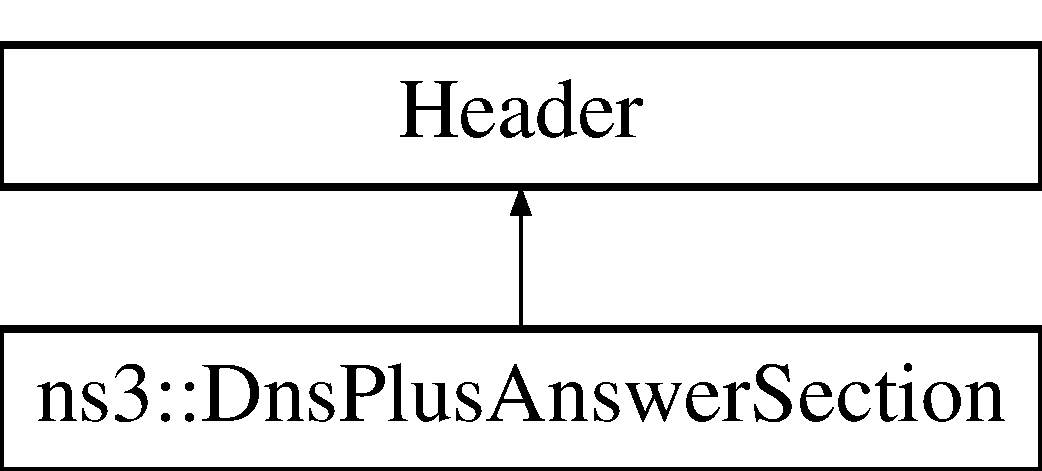
\includegraphics[height=2.000000cm]{classns3_1_1DnsPlusAnswerSection}
\end{center}
\end{figure}
\subsection*{Public Member Functions}
\begin{DoxyCompactItemize}
\item 
\hyperlink{classns3_1_1DnsPlusAnswerSection_aa1cb6dbcaa5dd169bb7059cb9e7f235f}{Dns\-Plus\-Answer\-Section} ()
\item 
virtual \hyperlink{classns3_1_1DnsPlusAnswerSection_ad0ace36d41761416f5920ef0126c3c1c}{$\sim$\-Dns\-Plus\-Answer\-Section} ()
\item 
virtual Type\-Id \hyperlink{classns3_1_1DnsPlusAnswerSection_a49405ae6e379132ec12836e371bc30ea}{Get\-Instance\-Type\-Id} (void) const 
\item 
virtual uint32\-\_\-t \hyperlink{classns3_1_1DnsPlusAnswerSection_a104fd989f35df0b3d4b85c33f73c864b}{Get\-Serialized\-Size} (void) const 
\item 
virtual void \hyperlink{classns3_1_1DnsPlusAnswerSection_a107a061aaef4face000adb7f3317f52e}{Serialize} (Buffer\-::\-Iterator start) const 
\item 
virtual uint32\-\_\-t \hyperlink{classns3_1_1DnsPlusAnswerSection_ad26bc4f46c7b59f1d296d903b3b88baf}{Deserialize} (Buffer\-::\-Iterator start)
\item 
virtual void \hyperlink{classns3_1_1DnsPlusAnswerSection_a34e5cbe940177587b43ba50d5586beee}{Print} (std\-::ostream \&os) const 
\item 
void \hyperlink{classns3_1_1DnsPlusAnswerSection_ab1fe1a8c00d52e81469d7edfa3d18b25}{Set\-Name} (std\-::string name)
\begin{DoxyCompactList}\small\item\em Set the name of the content in answer section. \end{DoxyCompactList}\item 
void \hyperlink{classns3_1_1DnsPlusAnswerSection_a4cfd46dc9b8003e1066d0501e2fefff4}{Set\-Name\-Length} (uint32\-\_\-t name\-Length)
\begin{DoxyCompactList}\small\item\em Set the length of the name of the content in answer section. \end{DoxyCompactList}\item 
void \hyperlink{classns3_1_1DnsPlusAnswerSection_a02c33fb6b02a6ace1f7a29e2df46960b}{Set\-Type} (uint16\-\_\-t Type)
\begin{DoxyCompactList}\small\item\em Set the type of data in R\-D D\-A\-T\-A field of answer section. \end{DoxyCompactList}\item 
void \hyperlink{classns3_1_1DnsPlusAnswerSection_ab1e5926e561e8728860024e0dd28a621}{Set\-Class} (uint16\-\_\-t Class)
\begin{DoxyCompactList}\small\item\em Set the class of data in R\-D D\-A\-T\-A field of answer section. \end{DoxyCompactList}\item 
void \hyperlink{classns3_1_1DnsPlusAnswerSection_a43fe4e27216871cb41e2aabd6ea41729}{Set\-Reserved\-Flag} (uint16\-\_\-t reserved\-Flag)
\begin{DoxyCompactList}\small\item\em Set the Reserved flag, these are not currently used, reserved for future use. \end{DoxyCompactList}\item 
void \hyperlink{classns3_1_1DnsPlusAnswerSection_a0eb309d8e58aac31bffa90518458de3b}{Set\-Ttl} (uint16\-\_\-t ttl)
\begin{DoxyCompactList}\small\item\em Set the ttl field of answer section. \end{DoxyCompactList}\item 
void \hyperlink{classns3_1_1DnsPlusAnswerSection_af7c04ba7137a994822eea5c9a2870ba1}{Set\-Rd\-Length} (uint16\-\_\-t rd\-Length)
\begin{DoxyCompactList}\small\item\em Set length of R\-D D\-A\-T\-A field of answer section. \end{DoxyCompactList}\item 
void \hyperlink{classns3_1_1DnsPlusAnswerSection_a9d577220126adbf68a0f6475b57560fb}{Set\-Rd\-Data} (Ipv4\-Address rd\-Data)
\begin{DoxyCompactList}\small\item\em Set the R\-D D\-A\-T\-A field of answer section. \end{DoxyCompactList}\item 
std\-::string \hyperlink{classns3_1_1DnsPlusAnswerSection_afdc38626ee1ff71c315bc2b6f119b350}{Get\-Name} ()
\begin{DoxyCompactList}\small\item\em Get name of the content. \end{DoxyCompactList}\item 
uint16\-\_\-t \hyperlink{classns3_1_1DnsPlusAnswerSection_ab1c3734345015e5178a41defed12e18e}{Get\-Class} ()
\begin{DoxyCompactList}\small\item\em Get the class of the answer section. \end{DoxyCompactList}\item 
uint16\-\_\-t \hyperlink{classns3_1_1DnsPlusAnswerSection_a766b46334b73e311f789842ba5e946d2}{Get\-Type} ()
\begin{DoxyCompactList}\small\item\em Get the type of answer section. \end{DoxyCompactList}\item 
uint8\-\_\-t \hyperlink{classns3_1_1DnsPlusAnswerSection_a0fcc7d52387c28ef0b6054a3d445bab2}{Get\-Reserved\-Flag} ()
\begin{DoxyCompactList}\small\item\em Get the reserved flag. \end{DoxyCompactList}\item 
uint16\-\_\-t \hyperlink{classns3_1_1DnsPlusAnswerSection_a675a24874435063a12abaacbf28caa7d}{Get\-Ttl} ()
\begin{DoxyCompactList}\small\item\em Get the ttl of answer section. \end{DoxyCompactList}\item 
uint16\-\_\-t \hyperlink{classns3_1_1DnsPlusAnswerSection_a7208ae0d866c3292f2b92de9f32fe869}{Get\-Rd\-Length} ()
\begin{DoxyCompactList}\small\item\em Get the length of R\-D Data of answer section. \end{DoxyCompactList}\item 
uint32\-\_\-t \hyperlink{classns3_1_1DnsPlusAnswerSection_ae3deac68a760812cbb49e532ac0ab2c6}{Get\-Rd\-Data} ()
\begin{DoxyCompactList}\small\item\em Get the R\-D Data of answer section. \end{DoxyCompactList}\item 
uint32\-\_\-t \hyperlink{classns3_1_1DnsPlusAnswerSection_a3f52e08f71e8f5d942c5c888e997ed5f}{Get\-Name\-Length} ()
\begin{DoxyCompactList}\small\item\em Get the Length of the name of the content. \end{DoxyCompactList}\end{DoxyCompactItemize}
\subsection*{Static Public Member Functions}
\begin{DoxyCompactItemize}
\item 
static Type\-Id \hyperlink{classns3_1_1DnsPlusAnswerSection_acc0093742dd85d654eb0faf7c3492baf}{Get\-Type\-Id} (void)
\begin{DoxyCompactList}\small\item\em Get the type I\-D. \end{DoxyCompactList}\end{DoxyCompactItemize}
\subsection*{Private Attributes}
\begin{DoxyCompactItemize}
\item 
uint8\-\_\-t \hyperlink{classns3_1_1DnsPlusAnswerSection_ab7c55e4309c4e3ea9d2f6cee4f51a5a9}{m\-\_\-reserved\-Flag}
\begin{DoxyCompactList}\small\item\em reserved flag bits \end{DoxyCompactList}\item 
std\-::string \hyperlink{classns3_1_1DnsPlusAnswerSection_a4e6ba01e32ecd32c175a814f60ddd315}{m\-\_\-name}
\begin{DoxyCompactList}\small\item\em name of the content \end{DoxyCompactList}\item 
uint16\-\_\-t \hyperlink{classns3_1_1DnsPlusAnswerSection_a9ea44f6d896057b365c56b947cd051b4}{m\-\_\-\-Class}
\begin{DoxyCompactList}\small\item\em class of data in R\-D D\-A\-T\-A field \end{DoxyCompactList}\item 
uint16\-\_\-t \hyperlink{classns3_1_1DnsPlusAnswerSection_aa1a416336d5681c959c988c299a6cddf}{m\-\_\-\-Type}
\begin{DoxyCompactList}\small\item\em type of data in R\-D D\-A\-T\-A field \end{DoxyCompactList}\item 
uint32\-\_\-t \hyperlink{classns3_1_1DnsPlusAnswerSection_ac7759da5ffc094ed4d0e60d7095ed1d2}{m\-\_\-name\-Length}
\begin{DoxyCompactList}\small\item\em length of the name of the content \end{DoxyCompactList}\item 
uint16\-\_\-t \hyperlink{classns3_1_1DnsPlusAnswerSection_a2b8a98168673224b6575ab009e883d2f}{m\-\_\-ttl}
\begin{DoxyCompactList}\small\item\em time to live of answer section \end{DoxyCompactList}\item 
uint16\-\_\-t \hyperlink{classns3_1_1DnsPlusAnswerSection_a87bd32bf4be3b0d809014553260f5abb}{m\-\_\-rd\-Length}
\begin{DoxyCompactList}\small\item\em length of R\-D Data \end{DoxyCompactList}\item 
uint32\-\_\-t \hyperlink{classns3_1_1DnsPlusAnswerSection_ab02f72df4dd55bc16b58c4915e7bc0ce}{m\-\_\-rd\-Data}
\begin{DoxyCompactList}\small\item\em R\-D Data of answer section. \end{DoxyCompactList}\end{DoxyCompactItemize}


\subsection{Detailed Description}
It is similar to D\-N\-S Answer Section header. 

I\-C\-N Manager send packet with this header to the source of the requested content. This header contains the ip address of the client to whom content has to be sent. 

\subsection{Constructor \& Destructor Documentation}
\hypertarget{classns3_1_1DnsPlusAnswerSection_aa1cb6dbcaa5dd169bb7059cb9e7f235f}{\index{ns3\-::\-Dns\-Plus\-Answer\-Section@{ns3\-::\-Dns\-Plus\-Answer\-Section}!Dns\-Plus\-Answer\-Section@{Dns\-Plus\-Answer\-Section}}
\index{Dns\-Plus\-Answer\-Section@{Dns\-Plus\-Answer\-Section}!ns3::DnsPlusAnswerSection@{ns3\-::\-Dns\-Plus\-Answer\-Section}}
\subsubsection[{Dns\-Plus\-Answer\-Section}]{\setlength{\rightskip}{0pt plus 5cm}ns3\-::\-Dns\-Plus\-Answer\-Section\-::\-Dns\-Plus\-Answer\-Section (
\begin{DoxyParamCaption}
{}
\end{DoxyParamCaption}
)}}\label{classns3_1_1DnsPlusAnswerSection_aa1cb6dbcaa5dd169bb7059cb9e7f235f}
\hypertarget{classns3_1_1DnsPlusAnswerSection_ad0ace36d41761416f5920ef0126c3c1c}{\index{ns3\-::\-Dns\-Plus\-Answer\-Section@{ns3\-::\-Dns\-Plus\-Answer\-Section}!$\sim$\-Dns\-Plus\-Answer\-Section@{$\sim$\-Dns\-Plus\-Answer\-Section}}
\index{$\sim$\-Dns\-Plus\-Answer\-Section@{$\sim$\-Dns\-Plus\-Answer\-Section}!ns3::DnsPlusAnswerSection@{ns3\-::\-Dns\-Plus\-Answer\-Section}}
\subsubsection[{$\sim$\-Dns\-Plus\-Answer\-Section}]{\setlength{\rightskip}{0pt plus 5cm}ns3\-::\-Dns\-Plus\-Answer\-Section\-::$\sim$\-Dns\-Plus\-Answer\-Section (
\begin{DoxyParamCaption}
{}
\end{DoxyParamCaption}
)\hspace{0.3cm}{\ttfamily [virtual]}}}\label{classns3_1_1DnsPlusAnswerSection_ad0ace36d41761416f5920ef0126c3c1c}


\subsection{Member Function Documentation}
\hypertarget{classns3_1_1DnsPlusAnswerSection_ad26bc4f46c7b59f1d296d903b3b88baf}{\index{ns3\-::\-Dns\-Plus\-Answer\-Section@{ns3\-::\-Dns\-Plus\-Answer\-Section}!Deserialize@{Deserialize}}
\index{Deserialize@{Deserialize}!ns3::DnsPlusAnswerSection@{ns3\-::\-Dns\-Plus\-Answer\-Section}}
\subsubsection[{Deserialize}]{\setlength{\rightskip}{0pt plus 5cm}uint32\-\_\-t ns3\-::\-Dns\-Plus\-Answer\-Section\-::\-Deserialize (
\begin{DoxyParamCaption}
\item[{Buffer\-::\-Iterator}]{start}
\end{DoxyParamCaption}
)\hspace{0.3cm}{\ttfamily [virtual]}}}\label{classns3_1_1DnsPlusAnswerSection_ad26bc4f46c7b59f1d296d903b3b88baf}
\hypertarget{classns3_1_1DnsPlusAnswerSection_ab1c3734345015e5178a41defed12e18e}{\index{ns3\-::\-Dns\-Plus\-Answer\-Section@{ns3\-::\-Dns\-Plus\-Answer\-Section}!Get\-Class@{Get\-Class}}
\index{Get\-Class@{Get\-Class}!ns3::DnsPlusAnswerSection@{ns3\-::\-Dns\-Plus\-Answer\-Section}}
\subsubsection[{Get\-Class}]{\setlength{\rightskip}{0pt plus 5cm}uint16\-\_\-t ns3\-::\-Dns\-Plus\-Answer\-Section\-::\-Get\-Class (
\begin{DoxyParamCaption}
{}
\end{DoxyParamCaption}
)}}\label{classns3_1_1DnsPlusAnswerSection_ab1c3734345015e5178a41defed12e18e}


Get the class of the answer section. 

\begin{DoxyReturn}{Returns}
class of answer section. 
\end{DoxyReturn}
\hypertarget{classns3_1_1DnsPlusAnswerSection_a49405ae6e379132ec12836e371bc30ea}{\index{ns3\-::\-Dns\-Plus\-Answer\-Section@{ns3\-::\-Dns\-Plus\-Answer\-Section}!Get\-Instance\-Type\-Id@{Get\-Instance\-Type\-Id}}
\index{Get\-Instance\-Type\-Id@{Get\-Instance\-Type\-Id}!ns3::DnsPlusAnswerSection@{ns3\-::\-Dns\-Plus\-Answer\-Section}}
\subsubsection[{Get\-Instance\-Type\-Id}]{\setlength{\rightskip}{0pt plus 5cm}Type\-Id ns3\-::\-Dns\-Plus\-Answer\-Section\-::\-Get\-Instance\-Type\-Id (
\begin{DoxyParamCaption}
\item[{void}]{}
\end{DoxyParamCaption}
) const\hspace{0.3cm}{\ttfamily [virtual]}}}\label{classns3_1_1DnsPlusAnswerSection_a49405ae6e379132ec12836e371bc30ea}
\hypertarget{classns3_1_1DnsPlusAnswerSection_afdc38626ee1ff71c315bc2b6f119b350}{\index{ns3\-::\-Dns\-Plus\-Answer\-Section@{ns3\-::\-Dns\-Plus\-Answer\-Section}!Get\-Name@{Get\-Name}}
\index{Get\-Name@{Get\-Name}!ns3::DnsPlusAnswerSection@{ns3\-::\-Dns\-Plus\-Answer\-Section}}
\subsubsection[{Get\-Name}]{\setlength{\rightskip}{0pt plus 5cm}std\-::string ns3\-::\-Dns\-Plus\-Answer\-Section\-::\-Get\-Name (
\begin{DoxyParamCaption}
{}
\end{DoxyParamCaption}
)}}\label{classns3_1_1DnsPlusAnswerSection_afdc38626ee1ff71c315bc2b6f119b350}


Get name of the content. 

\begin{DoxyReturn}{Returns}
name of the content. 
\end{DoxyReturn}
\hypertarget{classns3_1_1DnsPlusAnswerSection_a3f52e08f71e8f5d942c5c888e997ed5f}{\index{ns3\-::\-Dns\-Plus\-Answer\-Section@{ns3\-::\-Dns\-Plus\-Answer\-Section}!Get\-Name\-Length@{Get\-Name\-Length}}
\index{Get\-Name\-Length@{Get\-Name\-Length}!ns3::DnsPlusAnswerSection@{ns3\-::\-Dns\-Plus\-Answer\-Section}}
\subsubsection[{Get\-Name\-Length}]{\setlength{\rightskip}{0pt plus 5cm}uint32\-\_\-t ns3\-::\-Dns\-Plus\-Answer\-Section\-::\-Get\-Name\-Length (
\begin{DoxyParamCaption}
{}
\end{DoxyParamCaption}
)}}\label{classns3_1_1DnsPlusAnswerSection_a3f52e08f71e8f5d942c5c888e997ed5f}


Get the Length of the name of the content. 

\begin{DoxyReturn}{Returns}
length of the name of the content. 
\end{DoxyReturn}
\hypertarget{classns3_1_1DnsPlusAnswerSection_ae3deac68a760812cbb49e532ac0ab2c6}{\index{ns3\-::\-Dns\-Plus\-Answer\-Section@{ns3\-::\-Dns\-Plus\-Answer\-Section}!Get\-Rd\-Data@{Get\-Rd\-Data}}
\index{Get\-Rd\-Data@{Get\-Rd\-Data}!ns3::DnsPlusAnswerSection@{ns3\-::\-Dns\-Plus\-Answer\-Section}}
\subsubsection[{Get\-Rd\-Data}]{\setlength{\rightskip}{0pt plus 5cm}uint32\-\_\-t ns3\-::\-Dns\-Plus\-Answer\-Section\-::\-Get\-Rd\-Data (
\begin{DoxyParamCaption}
{}
\end{DoxyParamCaption}
)}}\label{classns3_1_1DnsPlusAnswerSection_ae3deac68a760812cbb49e532ac0ab2c6}


Get the R\-D Data of answer section. 

\begin{DoxyReturn}{Returns}
R\-D Data of answer section. 
\end{DoxyReturn}
\hypertarget{classns3_1_1DnsPlusAnswerSection_a7208ae0d866c3292f2b92de9f32fe869}{\index{ns3\-::\-Dns\-Plus\-Answer\-Section@{ns3\-::\-Dns\-Plus\-Answer\-Section}!Get\-Rd\-Length@{Get\-Rd\-Length}}
\index{Get\-Rd\-Length@{Get\-Rd\-Length}!ns3::DnsPlusAnswerSection@{ns3\-::\-Dns\-Plus\-Answer\-Section}}
\subsubsection[{Get\-Rd\-Length}]{\setlength{\rightskip}{0pt plus 5cm}uint16\-\_\-t ns3\-::\-Dns\-Plus\-Answer\-Section\-::\-Get\-Rd\-Length (
\begin{DoxyParamCaption}
{}
\end{DoxyParamCaption}
)}}\label{classns3_1_1DnsPlusAnswerSection_a7208ae0d866c3292f2b92de9f32fe869}


Get the length of R\-D Data of answer section. 

\begin{DoxyReturn}{Returns}
length of R\-D Data of answer section. 
\end{DoxyReturn}
\hypertarget{classns3_1_1DnsPlusAnswerSection_a0fcc7d52387c28ef0b6054a3d445bab2}{\index{ns3\-::\-Dns\-Plus\-Answer\-Section@{ns3\-::\-Dns\-Plus\-Answer\-Section}!Get\-Reserved\-Flag@{Get\-Reserved\-Flag}}
\index{Get\-Reserved\-Flag@{Get\-Reserved\-Flag}!ns3::DnsPlusAnswerSection@{ns3\-::\-Dns\-Plus\-Answer\-Section}}
\subsubsection[{Get\-Reserved\-Flag}]{\setlength{\rightskip}{0pt plus 5cm}uint8\-\_\-t ns3\-::\-Dns\-Plus\-Answer\-Section\-::\-Get\-Reserved\-Flag (
\begin{DoxyParamCaption}
{}
\end{DoxyParamCaption}
)}}\label{classns3_1_1DnsPlusAnswerSection_a0fcc7d52387c28ef0b6054a3d445bab2}


Get the reserved flag. 

\begin{DoxyReturn}{Returns}
reserved\-Flag of answer section. 
\end{DoxyReturn}
\hypertarget{classns3_1_1DnsPlusAnswerSection_a104fd989f35df0b3d4b85c33f73c864b}{\index{ns3\-::\-Dns\-Plus\-Answer\-Section@{ns3\-::\-Dns\-Plus\-Answer\-Section}!Get\-Serialized\-Size@{Get\-Serialized\-Size}}
\index{Get\-Serialized\-Size@{Get\-Serialized\-Size}!ns3::DnsPlusAnswerSection@{ns3\-::\-Dns\-Plus\-Answer\-Section}}
\subsubsection[{Get\-Serialized\-Size}]{\setlength{\rightskip}{0pt plus 5cm}uint32\-\_\-t ns3\-::\-Dns\-Plus\-Answer\-Section\-::\-Get\-Serialized\-Size (
\begin{DoxyParamCaption}
\item[{void}]{}
\end{DoxyParamCaption}
) const\hspace{0.3cm}{\ttfamily [virtual]}}}\label{classns3_1_1DnsPlusAnswerSection_a104fd989f35df0b3d4b85c33f73c864b}
\hypertarget{classns3_1_1DnsPlusAnswerSection_a675a24874435063a12abaacbf28caa7d}{\index{ns3\-::\-Dns\-Plus\-Answer\-Section@{ns3\-::\-Dns\-Plus\-Answer\-Section}!Get\-Ttl@{Get\-Ttl}}
\index{Get\-Ttl@{Get\-Ttl}!ns3::DnsPlusAnswerSection@{ns3\-::\-Dns\-Plus\-Answer\-Section}}
\subsubsection[{Get\-Ttl}]{\setlength{\rightskip}{0pt plus 5cm}uint16\-\_\-t ns3\-::\-Dns\-Plus\-Answer\-Section\-::\-Get\-Ttl (
\begin{DoxyParamCaption}
{}
\end{DoxyParamCaption}
)}}\label{classns3_1_1DnsPlusAnswerSection_a675a24874435063a12abaacbf28caa7d}


Get the ttl of answer section. 

\begin{DoxyReturn}{Returns}
ttl of answer section. 
\end{DoxyReturn}
\hypertarget{classns3_1_1DnsPlusAnswerSection_a766b46334b73e311f789842ba5e946d2}{\index{ns3\-::\-Dns\-Plus\-Answer\-Section@{ns3\-::\-Dns\-Plus\-Answer\-Section}!Get\-Type@{Get\-Type}}
\index{Get\-Type@{Get\-Type}!ns3::DnsPlusAnswerSection@{ns3\-::\-Dns\-Plus\-Answer\-Section}}
\subsubsection[{Get\-Type}]{\setlength{\rightskip}{0pt plus 5cm}uint16\-\_\-t ns3\-::\-Dns\-Plus\-Answer\-Section\-::\-Get\-Type (
\begin{DoxyParamCaption}
{}
\end{DoxyParamCaption}
)}}\label{classns3_1_1DnsPlusAnswerSection_a766b46334b73e311f789842ba5e946d2}


Get the type of answer section. 

\begin{DoxyReturn}{Returns}
type of answer section. 
\end{DoxyReturn}
\hypertarget{classns3_1_1DnsPlusAnswerSection_acc0093742dd85d654eb0faf7c3492baf}{\index{ns3\-::\-Dns\-Plus\-Answer\-Section@{ns3\-::\-Dns\-Plus\-Answer\-Section}!Get\-Type\-Id@{Get\-Type\-Id}}
\index{Get\-Type\-Id@{Get\-Type\-Id}!ns3::DnsPlusAnswerSection@{ns3\-::\-Dns\-Plus\-Answer\-Section}}
\subsubsection[{Get\-Type\-Id}]{\setlength{\rightskip}{0pt plus 5cm}Type\-Id ns3\-::\-Dns\-Plus\-Answer\-Section\-::\-Get\-Type\-Id (
\begin{DoxyParamCaption}
\item[{void}]{}
\end{DoxyParamCaption}
)\hspace{0.3cm}{\ttfamily [static]}}}\label{classns3_1_1DnsPlusAnswerSection_acc0093742dd85d654eb0faf7c3492baf}


Get the type I\-D. 

\begin{DoxyReturn}{Returns}
the object Type\-Id. 
\end{DoxyReturn}
\hypertarget{classns3_1_1DnsPlusAnswerSection_a34e5cbe940177587b43ba50d5586beee}{\index{ns3\-::\-Dns\-Plus\-Answer\-Section@{ns3\-::\-Dns\-Plus\-Answer\-Section}!Print@{Print}}
\index{Print@{Print}!ns3::DnsPlusAnswerSection@{ns3\-::\-Dns\-Plus\-Answer\-Section}}
\subsubsection[{Print}]{\setlength{\rightskip}{0pt plus 5cm}void ns3\-::\-Dns\-Plus\-Answer\-Section\-::\-Print (
\begin{DoxyParamCaption}
\item[{std\-::ostream \&}]{os}
\end{DoxyParamCaption}
) const\hspace{0.3cm}{\ttfamily [virtual]}}}\label{classns3_1_1DnsPlusAnswerSection_a34e5cbe940177587b43ba50d5586beee}
\hypertarget{classns3_1_1DnsPlusAnswerSection_a107a061aaef4face000adb7f3317f52e}{\index{ns3\-::\-Dns\-Plus\-Answer\-Section@{ns3\-::\-Dns\-Plus\-Answer\-Section}!Serialize@{Serialize}}
\index{Serialize@{Serialize}!ns3::DnsPlusAnswerSection@{ns3\-::\-Dns\-Plus\-Answer\-Section}}
\subsubsection[{Serialize}]{\setlength{\rightskip}{0pt plus 5cm}void ns3\-::\-Dns\-Plus\-Answer\-Section\-::\-Serialize (
\begin{DoxyParamCaption}
\item[{Buffer\-::\-Iterator}]{start}
\end{DoxyParamCaption}
) const\hspace{0.3cm}{\ttfamily [virtual]}}}\label{classns3_1_1DnsPlusAnswerSection_a107a061aaef4face000adb7f3317f52e}
\hypertarget{classns3_1_1DnsPlusAnswerSection_ab1e5926e561e8728860024e0dd28a621}{\index{ns3\-::\-Dns\-Plus\-Answer\-Section@{ns3\-::\-Dns\-Plus\-Answer\-Section}!Set\-Class@{Set\-Class}}
\index{Set\-Class@{Set\-Class}!ns3::DnsPlusAnswerSection@{ns3\-::\-Dns\-Plus\-Answer\-Section}}
\subsubsection[{Set\-Class}]{\setlength{\rightskip}{0pt plus 5cm}void ns3\-::\-Dns\-Plus\-Answer\-Section\-::\-Set\-Class (
\begin{DoxyParamCaption}
\item[{uint16\-\_\-t}]{Class}
\end{DoxyParamCaption}
)}}\label{classns3_1_1DnsPlusAnswerSection_ab1e5926e561e8728860024e0dd28a621}


Set the class of data in R\-D D\-A\-T\-A field of answer section. 


\begin{DoxyParams}{Parameters}
{\em class} & class of data in R\-D D\-A\-T\-A field of answer section. \\
\hline
\end{DoxyParams}
\hypertarget{classns3_1_1DnsPlusAnswerSection_ab1fe1a8c00d52e81469d7edfa3d18b25}{\index{ns3\-::\-Dns\-Plus\-Answer\-Section@{ns3\-::\-Dns\-Plus\-Answer\-Section}!Set\-Name@{Set\-Name}}
\index{Set\-Name@{Set\-Name}!ns3::DnsPlusAnswerSection@{ns3\-::\-Dns\-Plus\-Answer\-Section}}
\subsubsection[{Set\-Name}]{\setlength{\rightskip}{0pt plus 5cm}void ns3\-::\-Dns\-Plus\-Answer\-Section\-::\-Set\-Name (
\begin{DoxyParamCaption}
\item[{std\-::string}]{name}
\end{DoxyParamCaption}
)}}\label{classns3_1_1DnsPlusAnswerSection_ab1fe1a8c00d52e81469d7edfa3d18b25}


Set the name of the content in answer section. 


\begin{DoxyParams}{Parameters}
{\em name} & it is name of the content. \\
\hline
\end{DoxyParams}
\hypertarget{classns3_1_1DnsPlusAnswerSection_a4cfd46dc9b8003e1066d0501e2fefff4}{\index{ns3\-::\-Dns\-Plus\-Answer\-Section@{ns3\-::\-Dns\-Plus\-Answer\-Section}!Set\-Name\-Length@{Set\-Name\-Length}}
\index{Set\-Name\-Length@{Set\-Name\-Length}!ns3::DnsPlusAnswerSection@{ns3\-::\-Dns\-Plus\-Answer\-Section}}
\subsubsection[{Set\-Name\-Length}]{\setlength{\rightskip}{0pt plus 5cm}void ns3\-::\-Dns\-Plus\-Answer\-Section\-::\-Set\-Name\-Length (
\begin{DoxyParamCaption}
\item[{uint32\-\_\-t}]{name\-Length}
\end{DoxyParamCaption}
)}}\label{classns3_1_1DnsPlusAnswerSection_a4cfd46dc9b8003e1066d0501e2fefff4}


Set the length of the name of the content in answer section. 


\begin{DoxyParams}{Parameters}
{\em name\-Length} & length of the name of the content. \\
\hline
\end{DoxyParams}
\hypertarget{classns3_1_1DnsPlusAnswerSection_a9d577220126adbf68a0f6475b57560fb}{\index{ns3\-::\-Dns\-Plus\-Answer\-Section@{ns3\-::\-Dns\-Plus\-Answer\-Section}!Set\-Rd\-Data@{Set\-Rd\-Data}}
\index{Set\-Rd\-Data@{Set\-Rd\-Data}!ns3::DnsPlusAnswerSection@{ns3\-::\-Dns\-Plus\-Answer\-Section}}
\subsubsection[{Set\-Rd\-Data}]{\setlength{\rightskip}{0pt plus 5cm}void ns3\-::\-Dns\-Plus\-Answer\-Section\-::\-Set\-Rd\-Data (
\begin{DoxyParamCaption}
\item[{Ipv4\-Address}]{rd\-Data}
\end{DoxyParamCaption}
)}}\label{classns3_1_1DnsPlusAnswerSection_a9d577220126adbf68a0f6475b57560fb}


Set the R\-D D\-A\-T\-A field of answer section. 


\begin{DoxyParams}{Parameters}
{\em rd\-Data} & value of data in R\-D D\-A\-T\-A field of answer section. \\
\hline
\end{DoxyParams}
\hypertarget{classns3_1_1DnsPlusAnswerSection_af7c04ba7137a994822eea5c9a2870ba1}{\index{ns3\-::\-Dns\-Plus\-Answer\-Section@{ns3\-::\-Dns\-Plus\-Answer\-Section}!Set\-Rd\-Length@{Set\-Rd\-Length}}
\index{Set\-Rd\-Length@{Set\-Rd\-Length}!ns3::DnsPlusAnswerSection@{ns3\-::\-Dns\-Plus\-Answer\-Section}}
\subsubsection[{Set\-Rd\-Length}]{\setlength{\rightskip}{0pt plus 5cm}void ns3\-::\-Dns\-Plus\-Answer\-Section\-::\-Set\-Rd\-Length (
\begin{DoxyParamCaption}
\item[{uint16\-\_\-t}]{rd\-Length}
\end{DoxyParamCaption}
)}}\label{classns3_1_1DnsPlusAnswerSection_af7c04ba7137a994822eea5c9a2870ba1}


Set length of R\-D D\-A\-T\-A field of answer section. 


\begin{DoxyParams}{Parameters}
{\em rd\-Length} & length of R\-D D\-A\-T\-A field of answer section. \\
\hline
\end{DoxyParams}
\hypertarget{classns3_1_1DnsPlusAnswerSection_a43fe4e27216871cb41e2aabd6ea41729}{\index{ns3\-::\-Dns\-Plus\-Answer\-Section@{ns3\-::\-Dns\-Plus\-Answer\-Section}!Set\-Reserved\-Flag@{Set\-Reserved\-Flag}}
\index{Set\-Reserved\-Flag@{Set\-Reserved\-Flag}!ns3::DnsPlusAnswerSection@{ns3\-::\-Dns\-Plus\-Answer\-Section}}
\subsubsection[{Set\-Reserved\-Flag}]{\setlength{\rightskip}{0pt plus 5cm}void ns3\-::\-Dns\-Plus\-Answer\-Section\-::\-Set\-Reserved\-Flag (
\begin{DoxyParamCaption}
\item[{uint16\-\_\-t}]{reserved\-Flag}
\end{DoxyParamCaption}
)}}\label{classns3_1_1DnsPlusAnswerSection_a43fe4e27216871cb41e2aabd6ea41729}


Set the Reserved flag, these are not currently used, reserved for future use. 


\begin{DoxyParams}{Parameters}
{\em reserved\-Flag} & reserved flag bit \\
\hline
\end{DoxyParams}
\hypertarget{classns3_1_1DnsPlusAnswerSection_a0eb309d8e58aac31bffa90518458de3b}{\index{ns3\-::\-Dns\-Plus\-Answer\-Section@{ns3\-::\-Dns\-Plus\-Answer\-Section}!Set\-Ttl@{Set\-Ttl}}
\index{Set\-Ttl@{Set\-Ttl}!ns3::DnsPlusAnswerSection@{ns3\-::\-Dns\-Plus\-Answer\-Section}}
\subsubsection[{Set\-Ttl}]{\setlength{\rightskip}{0pt plus 5cm}void ns3\-::\-Dns\-Plus\-Answer\-Section\-::\-Set\-Ttl (
\begin{DoxyParamCaption}
\item[{uint16\-\_\-t}]{ttl}
\end{DoxyParamCaption}
)}}\label{classns3_1_1DnsPlusAnswerSection_a0eb309d8e58aac31bffa90518458de3b}


Set the ttl field of answer section. 


\begin{DoxyParams}{Parameters}
{\em ttl} & ttl field of answer section. \\
\hline
\end{DoxyParams}
\hypertarget{classns3_1_1DnsPlusAnswerSection_a02c33fb6b02a6ace1f7a29e2df46960b}{\index{ns3\-::\-Dns\-Plus\-Answer\-Section@{ns3\-::\-Dns\-Plus\-Answer\-Section}!Set\-Type@{Set\-Type}}
\index{Set\-Type@{Set\-Type}!ns3::DnsPlusAnswerSection@{ns3\-::\-Dns\-Plus\-Answer\-Section}}
\subsubsection[{Set\-Type}]{\setlength{\rightskip}{0pt plus 5cm}void ns3\-::\-Dns\-Plus\-Answer\-Section\-::\-Set\-Type (
\begin{DoxyParamCaption}
\item[{uint16\-\_\-t}]{Type}
\end{DoxyParamCaption}
)}}\label{classns3_1_1DnsPlusAnswerSection_a02c33fb6b02a6ace1f7a29e2df46960b}


Set the type of data in R\-D D\-A\-T\-A field of answer section. 


\begin{DoxyParams}{Parameters}
{\em type} & type of data in R\-D D\-A\-T\-A field of answer section. \\
\hline
\end{DoxyParams}


\subsection{Member Data Documentation}
\hypertarget{classns3_1_1DnsPlusAnswerSection_a9ea44f6d896057b365c56b947cd051b4}{\index{ns3\-::\-Dns\-Plus\-Answer\-Section@{ns3\-::\-Dns\-Plus\-Answer\-Section}!m\-\_\-\-Class@{m\-\_\-\-Class}}
\index{m\-\_\-\-Class@{m\-\_\-\-Class}!ns3::DnsPlusAnswerSection@{ns3\-::\-Dns\-Plus\-Answer\-Section}}
\subsubsection[{m\-\_\-\-Class}]{\setlength{\rightskip}{0pt plus 5cm}uint16\-\_\-t ns3\-::\-Dns\-Plus\-Answer\-Section\-::m\-\_\-\-Class\hspace{0.3cm}{\ttfamily [private]}}}\label{classns3_1_1DnsPlusAnswerSection_a9ea44f6d896057b365c56b947cd051b4}


class of data in R\-D D\-A\-T\-A field 

\hypertarget{classns3_1_1DnsPlusAnswerSection_a4e6ba01e32ecd32c175a814f60ddd315}{\index{ns3\-::\-Dns\-Plus\-Answer\-Section@{ns3\-::\-Dns\-Plus\-Answer\-Section}!m\-\_\-name@{m\-\_\-name}}
\index{m\-\_\-name@{m\-\_\-name}!ns3::DnsPlusAnswerSection@{ns3\-::\-Dns\-Plus\-Answer\-Section}}
\subsubsection[{m\-\_\-name}]{\setlength{\rightskip}{0pt plus 5cm}std\-::string ns3\-::\-Dns\-Plus\-Answer\-Section\-::m\-\_\-name\hspace{0.3cm}{\ttfamily [private]}}}\label{classns3_1_1DnsPlusAnswerSection_a4e6ba01e32ecd32c175a814f60ddd315}


name of the content 

\hypertarget{classns3_1_1DnsPlusAnswerSection_ac7759da5ffc094ed4d0e60d7095ed1d2}{\index{ns3\-::\-Dns\-Plus\-Answer\-Section@{ns3\-::\-Dns\-Plus\-Answer\-Section}!m\-\_\-name\-Length@{m\-\_\-name\-Length}}
\index{m\-\_\-name\-Length@{m\-\_\-name\-Length}!ns3::DnsPlusAnswerSection@{ns3\-::\-Dns\-Plus\-Answer\-Section}}
\subsubsection[{m\-\_\-name\-Length}]{\setlength{\rightskip}{0pt plus 5cm}uint32\-\_\-t ns3\-::\-Dns\-Plus\-Answer\-Section\-::m\-\_\-name\-Length\hspace{0.3cm}{\ttfamily [private]}}}\label{classns3_1_1DnsPlusAnswerSection_ac7759da5ffc094ed4d0e60d7095ed1d2}


length of the name of the content 

\hypertarget{classns3_1_1DnsPlusAnswerSection_ab02f72df4dd55bc16b58c4915e7bc0ce}{\index{ns3\-::\-Dns\-Plus\-Answer\-Section@{ns3\-::\-Dns\-Plus\-Answer\-Section}!m\-\_\-rd\-Data@{m\-\_\-rd\-Data}}
\index{m\-\_\-rd\-Data@{m\-\_\-rd\-Data}!ns3::DnsPlusAnswerSection@{ns3\-::\-Dns\-Plus\-Answer\-Section}}
\subsubsection[{m\-\_\-rd\-Data}]{\setlength{\rightskip}{0pt plus 5cm}uint32\-\_\-t ns3\-::\-Dns\-Plus\-Answer\-Section\-::m\-\_\-rd\-Data\hspace{0.3cm}{\ttfamily [private]}}}\label{classns3_1_1DnsPlusAnswerSection_ab02f72df4dd55bc16b58c4915e7bc0ce}


R\-D Data of answer section. 

\hypertarget{classns3_1_1DnsPlusAnswerSection_a87bd32bf4be3b0d809014553260f5abb}{\index{ns3\-::\-Dns\-Plus\-Answer\-Section@{ns3\-::\-Dns\-Plus\-Answer\-Section}!m\-\_\-rd\-Length@{m\-\_\-rd\-Length}}
\index{m\-\_\-rd\-Length@{m\-\_\-rd\-Length}!ns3::DnsPlusAnswerSection@{ns3\-::\-Dns\-Plus\-Answer\-Section}}
\subsubsection[{m\-\_\-rd\-Length}]{\setlength{\rightskip}{0pt plus 5cm}uint16\-\_\-t ns3\-::\-Dns\-Plus\-Answer\-Section\-::m\-\_\-rd\-Length\hspace{0.3cm}{\ttfamily [private]}}}\label{classns3_1_1DnsPlusAnswerSection_a87bd32bf4be3b0d809014553260f5abb}


length of R\-D Data 

\hypertarget{classns3_1_1DnsPlusAnswerSection_ab7c55e4309c4e3ea9d2f6cee4f51a5a9}{\index{ns3\-::\-Dns\-Plus\-Answer\-Section@{ns3\-::\-Dns\-Plus\-Answer\-Section}!m\-\_\-reserved\-Flag@{m\-\_\-reserved\-Flag}}
\index{m\-\_\-reserved\-Flag@{m\-\_\-reserved\-Flag}!ns3::DnsPlusAnswerSection@{ns3\-::\-Dns\-Plus\-Answer\-Section}}
\subsubsection[{m\-\_\-reserved\-Flag}]{\setlength{\rightskip}{0pt plus 5cm}uint8\-\_\-t ns3\-::\-Dns\-Plus\-Answer\-Section\-::m\-\_\-reserved\-Flag\hspace{0.3cm}{\ttfamily [private]}}}\label{classns3_1_1DnsPlusAnswerSection_ab7c55e4309c4e3ea9d2f6cee4f51a5a9}


reserved flag bits 

\hypertarget{classns3_1_1DnsPlusAnswerSection_a2b8a98168673224b6575ab009e883d2f}{\index{ns3\-::\-Dns\-Plus\-Answer\-Section@{ns3\-::\-Dns\-Plus\-Answer\-Section}!m\-\_\-ttl@{m\-\_\-ttl}}
\index{m\-\_\-ttl@{m\-\_\-ttl}!ns3::DnsPlusAnswerSection@{ns3\-::\-Dns\-Plus\-Answer\-Section}}
\subsubsection[{m\-\_\-ttl}]{\setlength{\rightskip}{0pt plus 5cm}uint16\-\_\-t ns3\-::\-Dns\-Plus\-Answer\-Section\-::m\-\_\-ttl\hspace{0.3cm}{\ttfamily [private]}}}\label{classns3_1_1DnsPlusAnswerSection_a2b8a98168673224b6575ab009e883d2f}


time to live of answer section 

\hypertarget{classns3_1_1DnsPlusAnswerSection_aa1a416336d5681c959c988c299a6cddf}{\index{ns3\-::\-Dns\-Plus\-Answer\-Section@{ns3\-::\-Dns\-Plus\-Answer\-Section}!m\-\_\-\-Type@{m\-\_\-\-Type}}
\index{m\-\_\-\-Type@{m\-\_\-\-Type}!ns3::DnsPlusAnswerSection@{ns3\-::\-Dns\-Plus\-Answer\-Section}}
\subsubsection[{m\-\_\-\-Type}]{\setlength{\rightskip}{0pt plus 5cm}uint16\-\_\-t ns3\-::\-Dns\-Plus\-Answer\-Section\-::m\-\_\-\-Type\hspace{0.3cm}{\ttfamily [private]}}}\label{classns3_1_1DnsPlusAnswerSection_aa1a416336d5681c959c988c299a6cddf}


type of data in R\-D D\-A\-T\-A field 



The documentation for this class was generated from the following files\-:\begin{DoxyCompactItemize}
\item 
model/\hyperlink{dnsplus-answer-section_8h}{dnsplus-\/answer-\/section.\-h}\item 
model/\hyperlink{dnsplus-answer-section_8cc}{dnsplus-\/answer-\/section.\-cc}\end{DoxyCompactItemize}

\hypertarget{classns3_1_1DnsPlusHeader}{\section{ns3\-:\-:Dns\-Plus\-Header Class Reference}
\label{classns3_1_1DnsPlusHeader}\index{ns3\-::\-Dns\-Plus\-Header@{ns3\-::\-Dns\-Plus\-Header}}
}


It is similar to D\-N\-S header. It used for name resolution of the content.  




{\ttfamily \#include $<$dnsplus-\/header.\-h$>$}

Inheritance diagram for ns3\-:\-:Dns\-Plus\-Header\-:\begin{figure}[H]
\begin{center}
\leavevmode
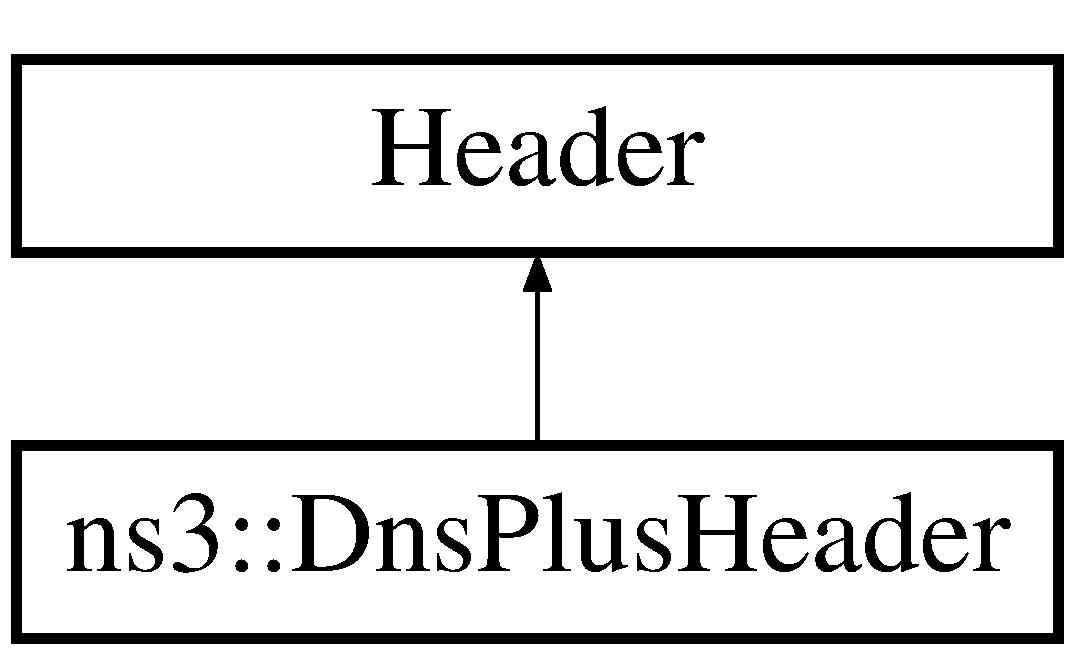
\includegraphics[height=2.000000cm]{classns3_1_1DnsPlusHeader}
\end{center}
\end{figure}
\subsection*{Public Member Functions}
\begin{DoxyCompactItemize}
\item 
\hyperlink{classns3_1_1DnsPlusHeader_aa39739cfaece6711a01861f45f0e6067}{Dns\-Plus\-Header} ()
\item 
\hyperlink{classns3_1_1DnsPlusHeader_a16cd6385e338fbb7cdcd0c6d33ccc7bb}{$\sim$\-Dns\-Plus\-Header} ()
\item 
virtual Type\-Id \hyperlink{classns3_1_1DnsPlusHeader_a4d290db0c63ed92adc4cdbd09fe84c24}{Get\-Instance\-Type\-Id} (void) const 
\item 
virtual uint32\-\_\-t \hyperlink{classns3_1_1DnsPlusHeader_ac951e2cb1473ec87540b829c2d572b39}{Get\-Serialized\-Size} (void) const 
\item 
virtual void \hyperlink{classns3_1_1DnsPlusHeader_af396f9396640c877af51efaf2f199072}{Serialize} (Buffer\-::\-Iterator start) const 
\item 
virtual uint32\-\_\-t \hyperlink{classns3_1_1DnsPlusHeader_a4fd5e5a6b42851c06ddf3aec0e357768}{Deserialize} (Buffer\-::\-Iterator start)
\item 
virtual void \hyperlink{classns3_1_1DnsPlusHeader_a1db3739a5909bf66de04839fd455c244}{Print} (std\-::ostream \&os) const 
\item 
void \hyperlink{classns3_1_1DnsPlusHeader_a163bb071a4227854dcdd139c7f98cd27}{Set\-Q\-R} (uint8\-\_\-t qr\-Bit)
\begin{DoxyCompactList}\small\item\em Set Q\-R bit. \end{DoxyCompactList}\item 
void \hyperlink{classns3_1_1DnsPlusHeader_aaeb6a6c63353ba23e4b992f4bac58b05}{Set\-Id} (uint16\-\_\-t id\-Bits)
\begin{DoxyCompactList}\small\item\em Set Id. \end{DoxyCompactList}\item 
void \hyperlink{classns3_1_1DnsPlusHeader_a3b6ee82ad16a50f44ee634477e73b560}{Set\-O\-P\-C\-O\-D\-E} (uint8\-\_\-t opcode)
\begin{DoxyCompactList}\small\item\em Set opcode. \end{DoxyCompactList}\item 
void \hyperlink{classns3_1_1DnsPlusHeader_a101aaca4f9508380a7bb27b170de4c9f}{Set\-A\-A} (uint8\-\_\-t aa\-Bit)
\begin{DoxyCompactList}\small\item\em Set A\-A Authoritative Answer bit. \end{DoxyCompactList}\item 
void \hyperlink{classns3_1_1DnsPlusHeader_a5902c88c45f698ddea33524ab548a7d9}{Set\-T\-C} (uint8\-\_\-t tc\-Bit)
\begin{DoxyCompactList}\small\item\em Set Truncation bit. \end{DoxyCompactList}\item 
void \hyperlink{classns3_1_1DnsPlusHeader_ad7e284af8733c294da48aa30a6587233}{Set\-R\-D} (uint8\-\_\-t rd\-Bit)
\begin{DoxyCompactList}\small\item\em Set Recursion Desired bit. \end{DoxyCompactList}\item 
void \hyperlink{classns3_1_1DnsPlusHeader_ae3027f5af8724d06e2e1df355ae0a853}{Set\-R\-A} (uint8\-\_\-t ra\-Bit)
\begin{DoxyCompactList}\small\item\em Set Recursion Avaliable bit. \end{DoxyCompactList}\item 
void \hyperlink{classns3_1_1DnsPlusHeader_aae30ef6d451eec678278171ed7a5fe6c}{Set\-Z} (uint8\-\_\-t z\-Bit)
\begin{DoxyCompactList}\small\item\em Set Z bit. \end{DoxyCompactList}\item 
void \hyperlink{classns3_1_1DnsPlusHeader_a83fb23f26dc34870c1bf6e1284b32ef5}{Set\-R\-C\-O\-D\-E} (uint8\-\_\-t rcode\-Bits)
\begin{DoxyCompactList}\small\item\em Set Response Code. \end{DoxyCompactList}\item 
void \hyperlink{classns3_1_1DnsPlusHeader_a975e84f17140d5c7ba171edd64b7919e}{Set\-Q\-D\-Count} (uint16\-\_\-t qdcount\-Bits)
\begin{DoxyCompactList}\small\item\em Set Q\-D\-Count Bit. \end{DoxyCompactList}\item 
void \hyperlink{classns3_1_1DnsPlusHeader_a49a171a0aa8582dcf6a44bdfde783c7a}{Set\-A\-N\-Count} (uint16\-\_\-t ancount\-Bits)
\begin{DoxyCompactList}\small\item\em Set A\-N\-Count Bit. \end{DoxyCompactList}\item 
void \hyperlink{classns3_1_1DnsPlusHeader_aae6d4997842c4e7674eb5da84aca1758}{Set\-N\-S\-Count} (uint16\-\_\-t nscount\-Bits)
\begin{DoxyCompactList}\small\item\em Set N\-S\-Count bit. \end{DoxyCompactList}\item 
void \hyperlink{classns3_1_1DnsPlusHeader_a77392a980ddd74a651c6b91e3a68e7cf}{Set\-A\-R\-Count} (uint16\-\_\-t arcount\-Bits)
\begin{DoxyCompactList}\small\item\em Set A\-R\-Count Bit. \end{DoxyCompactList}\item 
uint16\-\_\-t \hyperlink{classns3_1_1DnsPlusHeader_aae7edb215fce7562cb0946b87f8f84d0}{Get\-Id} ()
\begin{DoxyCompactList}\small\item\em Get Id of D\-N\-S request. \end{DoxyCompactList}\item 
uint8\-\_\-t \hyperlink{classns3_1_1DnsPlusHeader_aed50596c87046b01e05bd9851a69e82c}{Get\-Q\-R} ()
\begin{DoxyCompactList}\small\item\em Get Q\-R bit. \end{DoxyCompactList}\item 
uint8\-\_\-t \hyperlink{classns3_1_1DnsPlusHeader_a7c1f46655a3b37ce288922a10c0b1d85}{Get\-O\-P\-C\-O\-D\-E} ()
\begin{DoxyCompactList}\small\item\em Get O\-P\-C\-O\-D\-E bits. \end{DoxyCompactList}\item 
uint8\-\_\-t \hyperlink{classns3_1_1DnsPlusHeader_a3134d8329f6b6d30398bd85fd5dc680b}{Get\-A\-A} ()
\begin{DoxyCompactList}\small\item\em Get A\-A bit. \end{DoxyCompactList}\item 
uint8\-\_\-t \hyperlink{classns3_1_1DnsPlusHeader_a63a67866520ddb9348b1177fe2fc3e3e}{Get\-T\-C} ()
\begin{DoxyCompactList}\small\item\em Get T\-C bit. \end{DoxyCompactList}\item 
uint8\-\_\-t \hyperlink{classns3_1_1DnsPlusHeader_a6ba87b0dbc7c2198670c6c4e31f9a726}{Get\-R\-D} ()
\begin{DoxyCompactList}\small\item\em Get R\-D bit. \end{DoxyCompactList}\item 
uint8\-\_\-t \hyperlink{classns3_1_1DnsPlusHeader_a0d9c76d160543f5d6bcc032c6d1e8994}{Get\-R\-A} ()
\begin{DoxyCompactList}\small\item\em Get R\-A bit. \end{DoxyCompactList}\item 
uint8\-\_\-t \hyperlink{classns3_1_1DnsPlusHeader_af00e13f343d53b2bb84079b850e88eb5}{Get\-Z} ()
\begin{DoxyCompactList}\small\item\em Get Z bit. \end{DoxyCompactList}\item 
uint8\-\_\-t \hyperlink{classns3_1_1DnsPlusHeader_aa7f893eb6a224c347e11d5af5ec5e87c}{Get\-R\-C\-O\-D\-E} ()
\begin{DoxyCompactList}\small\item\em Get R\-C\-O\-D\-E. \end{DoxyCompactList}\item 
uint16\-\_\-t \hyperlink{classns3_1_1DnsPlusHeader_a72e660095dcbbcfbd3ea56af26081fde}{Get\-Q\-D\-Count} ()
\begin{DoxyCompactList}\small\item\em Get Q\-Dcount. \end{DoxyCompactList}\item 
uint16\-\_\-t \hyperlink{classns3_1_1DnsPlusHeader_ad4170edcd79f47db1d5d344265dbe814}{Get\-A\-N\-Count} ()
\begin{DoxyCompactList}\small\item\em Get A\-N\-Count. \end{DoxyCompactList}\item 
uint16\-\_\-t \hyperlink{classns3_1_1DnsPlusHeader_aabe109de0f4dd99b373f108b24a6f4dd}{Get\-N\-S\-Count} ()
\begin{DoxyCompactList}\small\item\em Get N\-Scount. \end{DoxyCompactList}\item 
uint16\-\_\-t \hyperlink{classns3_1_1DnsPlusHeader_a5a870a653b4cee6899e219510fbfa4a4}{Get\-A\-R\-Count} ()
\begin{DoxyCompactList}\small\item\em Get A\-R\-Count. \end{DoxyCompactList}\end{DoxyCompactItemize}
\subsection*{Static Public Member Functions}
\begin{DoxyCompactItemize}
\item 
static Type\-Id \hyperlink{classns3_1_1DnsPlusHeader_aca249927d0ab0ec498b4dd77c76fc9ec}{Get\-Type\-Id} (void)
\begin{DoxyCompactList}\small\item\em Get the type I\-D. \end{DoxyCompactList}\end{DoxyCompactItemize}
\subsection*{Private Attributes}
\begin{DoxyCompactItemize}
\item 
uint32\-\_\-t \hyperlink{classns3_1_1DnsPlusHeader_a2cb95f6912613452fc57847e15e4f7ac}{m\-\_\-flag}
\begin{DoxyCompactList}\small\item\em flag \end{DoxyCompactList}\item 
uint16\-\_\-t \hyperlink{classns3_1_1DnsPlusHeader_a5c9375cfe16fc339e52d0ae1b9c19a24}{m\-\_\-\-Id}
\begin{DoxyCompactList}\small\item\em Id bits of header. \end{DoxyCompactList}\item 
uint8\-\_\-t \hyperlink{classns3_1_1DnsPlusHeader_a913492faf18c9740d1a4db2e7b056b54}{m\-\_\-\-Q\-R}
\begin{DoxyCompactList}\small\item\em Q\-R bit of header. \end{DoxyCompactList}\item 
uint8\-\_\-t \hyperlink{classns3_1_1DnsPlusHeader_ae93aeff5c9677e5252405cab8323f2df}{m\-\_\-\-O\-P\-C\-O\-D\-E}
\begin{DoxyCompactList}\small\item\em O\-P\-C\-O\-D\-E bits of header. \end{DoxyCompactList}\item 
uint8\-\_\-t \hyperlink{classns3_1_1DnsPlusHeader_a2e41f079b9f89209837405def7797a0d}{m\-\_\-\-A\-A}
\begin{DoxyCompactList}\small\item\em A\-A bit of header. \end{DoxyCompactList}\item 
uint8\-\_\-t \hyperlink{classns3_1_1DnsPlusHeader_ad6b32f1358164571eb3eba7f083af321}{m\-\_\-\-T\-C}
\begin{DoxyCompactList}\small\item\em T\-C bit of header. \end{DoxyCompactList}\item 
uint8\-\_\-t \hyperlink{classns3_1_1DnsPlusHeader_aceb20feea34744185f0e8fcb0ea4e7f4}{m\-\_\-\-R\-D}
\begin{DoxyCompactList}\small\item\em R\-D bit of header. \end{DoxyCompactList}\item 
uint8\-\_\-t \hyperlink{classns3_1_1DnsPlusHeader_a275459d7076136ce2c7099734b264cd5}{m\-\_\-\-R\-A}
\begin{DoxyCompactList}\small\item\em R\-A bit of header. \end{DoxyCompactList}\item 
uint8\-\_\-t \hyperlink{classns3_1_1DnsPlusHeader_a9fb25d01e3e4ce98158926c2195a20cf}{m\-\_\-\-Z}
\begin{DoxyCompactList}\small\item\em Z bits of header. \end{DoxyCompactList}\item 
uint8\-\_\-t \hyperlink{classns3_1_1DnsPlusHeader_a35835f0ee81cfec4806f85d9b62daca6}{m\-\_\-\-R\-C\-O\-D\-E}
\begin{DoxyCompactList}\small\item\em R\-C\-O\-D\-E bits of header. \end{DoxyCompactList}\item 
uint16\-\_\-t \hyperlink{classns3_1_1DnsPlusHeader_ab85daf2b1bc16d2c58d1b6c1e21395d8}{m\-\_\-\-Q\-D\-Count}
\begin{DoxyCompactList}\small\item\em Q\-D\-Count bits of header. \end{DoxyCompactList}\item 
uint16\-\_\-t \hyperlink{classns3_1_1DnsPlusHeader_ac01fe04b25d9e3e75a4ae181cc8a156f}{m\-\_\-\-A\-N\-Count}
\begin{DoxyCompactList}\small\item\em A\-N\-Count bits of header. \end{DoxyCompactList}\item 
uint16\-\_\-t \hyperlink{classns3_1_1DnsPlusHeader_ace416d666df5fe25acfbfdd7aad309ce}{m\-\_\-\-N\-S\-Count}
\begin{DoxyCompactList}\small\item\em N\-S\-Count bits of header. \end{DoxyCompactList}\item 
uint16\-\_\-t \hyperlink{classns3_1_1DnsPlusHeader_afe7adb4352d8f52c21a7c3f922314045}{m\-\_\-\-A\-R\-Count}
\begin{DoxyCompactList}\small\item\em A\-R\-Count bits of header. \end{DoxyCompactList}\end{DoxyCompactItemize}


\subsection{Detailed Description}
It is similar to D\-N\-S header. It used for name resolution of the content. 

\subsection{Constructor \& Destructor Documentation}
\hypertarget{classns3_1_1DnsPlusHeader_aa39739cfaece6711a01861f45f0e6067}{\index{ns3\-::\-Dns\-Plus\-Header@{ns3\-::\-Dns\-Plus\-Header}!Dns\-Plus\-Header@{Dns\-Plus\-Header}}
\index{Dns\-Plus\-Header@{Dns\-Plus\-Header}!ns3::DnsPlusHeader@{ns3\-::\-Dns\-Plus\-Header}}
\subsubsection[{Dns\-Plus\-Header}]{\setlength{\rightskip}{0pt plus 5cm}ns3\-::\-Dns\-Plus\-Header\-::\-Dns\-Plus\-Header (
\begin{DoxyParamCaption}
{}
\end{DoxyParamCaption}
)}}\label{classns3_1_1DnsPlusHeader_aa39739cfaece6711a01861f45f0e6067}
\hypertarget{classns3_1_1DnsPlusHeader_a16cd6385e338fbb7cdcd0c6d33ccc7bb}{\index{ns3\-::\-Dns\-Plus\-Header@{ns3\-::\-Dns\-Plus\-Header}!$\sim$\-Dns\-Plus\-Header@{$\sim$\-Dns\-Plus\-Header}}
\index{$\sim$\-Dns\-Plus\-Header@{$\sim$\-Dns\-Plus\-Header}!ns3::DnsPlusHeader@{ns3\-::\-Dns\-Plus\-Header}}
\subsubsection[{$\sim$\-Dns\-Plus\-Header}]{\setlength{\rightskip}{0pt plus 5cm}ns3\-::\-Dns\-Plus\-Header\-::$\sim$\-Dns\-Plus\-Header (
\begin{DoxyParamCaption}
{}
\end{DoxyParamCaption}
)}}\label{classns3_1_1DnsPlusHeader_a16cd6385e338fbb7cdcd0c6d33ccc7bb}


\subsection{Member Function Documentation}
\hypertarget{classns3_1_1DnsPlusHeader_a4fd5e5a6b42851c06ddf3aec0e357768}{\index{ns3\-::\-Dns\-Plus\-Header@{ns3\-::\-Dns\-Plus\-Header}!Deserialize@{Deserialize}}
\index{Deserialize@{Deserialize}!ns3::DnsPlusHeader@{ns3\-::\-Dns\-Plus\-Header}}
\subsubsection[{Deserialize}]{\setlength{\rightskip}{0pt plus 5cm}uint32\-\_\-t ns3\-::\-Dns\-Plus\-Header\-::\-Deserialize (
\begin{DoxyParamCaption}
\item[{Buffer\-::\-Iterator}]{start}
\end{DoxyParamCaption}
)\hspace{0.3cm}{\ttfamily [virtual]}}}\label{classns3_1_1DnsPlusHeader_a4fd5e5a6b42851c06ddf3aec0e357768}
\hypertarget{classns3_1_1DnsPlusHeader_a3134d8329f6b6d30398bd85fd5dc680b}{\index{ns3\-::\-Dns\-Plus\-Header@{ns3\-::\-Dns\-Plus\-Header}!Get\-A\-A@{Get\-A\-A}}
\index{Get\-A\-A@{Get\-A\-A}!ns3::DnsPlusHeader@{ns3\-::\-Dns\-Plus\-Header}}
\subsubsection[{Get\-A\-A}]{\setlength{\rightskip}{0pt plus 5cm}uint8\-\_\-t ns3\-::\-Dns\-Plus\-Header\-::\-Get\-A\-A (
\begin{DoxyParamCaption}
{}
\end{DoxyParamCaption}
)}}\label{classns3_1_1DnsPlusHeader_a3134d8329f6b6d30398bd85fd5dc680b}


Get A\-A bit. 

\begin{DoxyReturn}{Returns}
A\-A bit 
\end{DoxyReturn}
\hypertarget{classns3_1_1DnsPlusHeader_ad4170edcd79f47db1d5d344265dbe814}{\index{ns3\-::\-Dns\-Plus\-Header@{ns3\-::\-Dns\-Plus\-Header}!Get\-A\-N\-Count@{Get\-A\-N\-Count}}
\index{Get\-A\-N\-Count@{Get\-A\-N\-Count}!ns3::DnsPlusHeader@{ns3\-::\-Dns\-Plus\-Header}}
\subsubsection[{Get\-A\-N\-Count}]{\setlength{\rightskip}{0pt plus 5cm}uint16\-\_\-t ns3\-::\-Dns\-Plus\-Header\-::\-Get\-A\-N\-Count (
\begin{DoxyParamCaption}
{}
\end{DoxyParamCaption}
)}}\label{classns3_1_1DnsPlusHeader_ad4170edcd79f47db1d5d344265dbe814}


Get A\-N\-Count. 

\begin{DoxyReturn}{Returns}
A\-N\-Count 
\end{DoxyReturn}
\hypertarget{classns3_1_1DnsPlusHeader_a5a870a653b4cee6899e219510fbfa4a4}{\index{ns3\-::\-Dns\-Plus\-Header@{ns3\-::\-Dns\-Plus\-Header}!Get\-A\-R\-Count@{Get\-A\-R\-Count}}
\index{Get\-A\-R\-Count@{Get\-A\-R\-Count}!ns3::DnsPlusHeader@{ns3\-::\-Dns\-Plus\-Header}}
\subsubsection[{Get\-A\-R\-Count}]{\setlength{\rightskip}{0pt plus 5cm}uint16\-\_\-t ns3\-::\-Dns\-Plus\-Header\-::\-Get\-A\-R\-Count (
\begin{DoxyParamCaption}
{}
\end{DoxyParamCaption}
)}}\label{classns3_1_1DnsPlusHeader_a5a870a653b4cee6899e219510fbfa4a4}


Get A\-R\-Count. 

\begin{DoxyReturn}{Returns}
A\-R\-Count bit 
\end{DoxyReturn}
\hypertarget{classns3_1_1DnsPlusHeader_aae7edb215fce7562cb0946b87f8f84d0}{\index{ns3\-::\-Dns\-Plus\-Header@{ns3\-::\-Dns\-Plus\-Header}!Get\-Id@{Get\-Id}}
\index{Get\-Id@{Get\-Id}!ns3::DnsPlusHeader@{ns3\-::\-Dns\-Plus\-Header}}
\subsubsection[{Get\-Id}]{\setlength{\rightskip}{0pt plus 5cm}uint16\-\_\-t ns3\-::\-Dns\-Plus\-Header\-::\-Get\-Id (
\begin{DoxyParamCaption}
{}
\end{DoxyParamCaption}
)}}\label{classns3_1_1DnsPlusHeader_aae7edb215fce7562cb0946b87f8f84d0}


Get Id of D\-N\-S request. 

\begin{DoxyReturn}{Returns}
Id of D\-N\-S request 
\end{DoxyReturn}
\hypertarget{classns3_1_1DnsPlusHeader_a4d290db0c63ed92adc4cdbd09fe84c24}{\index{ns3\-::\-Dns\-Plus\-Header@{ns3\-::\-Dns\-Plus\-Header}!Get\-Instance\-Type\-Id@{Get\-Instance\-Type\-Id}}
\index{Get\-Instance\-Type\-Id@{Get\-Instance\-Type\-Id}!ns3::DnsPlusHeader@{ns3\-::\-Dns\-Plus\-Header}}
\subsubsection[{Get\-Instance\-Type\-Id}]{\setlength{\rightskip}{0pt plus 5cm}Type\-Id ns3\-::\-Dns\-Plus\-Header\-::\-Get\-Instance\-Type\-Id (
\begin{DoxyParamCaption}
\item[{void}]{}
\end{DoxyParamCaption}
) const\hspace{0.3cm}{\ttfamily [virtual]}}}\label{classns3_1_1DnsPlusHeader_a4d290db0c63ed92adc4cdbd09fe84c24}
\hypertarget{classns3_1_1DnsPlusHeader_aabe109de0f4dd99b373f108b24a6f4dd}{\index{ns3\-::\-Dns\-Plus\-Header@{ns3\-::\-Dns\-Plus\-Header}!Get\-N\-S\-Count@{Get\-N\-S\-Count}}
\index{Get\-N\-S\-Count@{Get\-N\-S\-Count}!ns3::DnsPlusHeader@{ns3\-::\-Dns\-Plus\-Header}}
\subsubsection[{Get\-N\-S\-Count}]{\setlength{\rightskip}{0pt plus 5cm}uint16\-\_\-t ns3\-::\-Dns\-Plus\-Header\-::\-Get\-N\-S\-Count (
\begin{DoxyParamCaption}
{}
\end{DoxyParamCaption}
)}}\label{classns3_1_1DnsPlusHeader_aabe109de0f4dd99b373f108b24a6f4dd}


Get N\-Scount. 

\begin{DoxyReturn}{Returns}
N\-S\-Count bit 
\end{DoxyReturn}
\hypertarget{classns3_1_1DnsPlusHeader_a7c1f46655a3b37ce288922a10c0b1d85}{\index{ns3\-::\-Dns\-Plus\-Header@{ns3\-::\-Dns\-Plus\-Header}!Get\-O\-P\-C\-O\-D\-E@{Get\-O\-P\-C\-O\-D\-E}}
\index{Get\-O\-P\-C\-O\-D\-E@{Get\-O\-P\-C\-O\-D\-E}!ns3::DnsPlusHeader@{ns3\-::\-Dns\-Plus\-Header}}
\subsubsection[{Get\-O\-P\-C\-O\-D\-E}]{\setlength{\rightskip}{0pt plus 5cm}uint8\-\_\-t ns3\-::\-Dns\-Plus\-Header\-::\-Get\-O\-P\-C\-O\-D\-E (
\begin{DoxyParamCaption}
{}
\end{DoxyParamCaption}
)}}\label{classns3_1_1DnsPlusHeader_a7c1f46655a3b37ce288922a10c0b1d85}


Get O\-P\-C\-O\-D\-E bits. 

\begin{DoxyReturn}{Returns}
O\-P\-C\-O\-D\-E bits 
\end{DoxyReturn}
\hypertarget{classns3_1_1DnsPlusHeader_a72e660095dcbbcfbd3ea56af26081fde}{\index{ns3\-::\-Dns\-Plus\-Header@{ns3\-::\-Dns\-Plus\-Header}!Get\-Q\-D\-Count@{Get\-Q\-D\-Count}}
\index{Get\-Q\-D\-Count@{Get\-Q\-D\-Count}!ns3::DnsPlusHeader@{ns3\-::\-Dns\-Plus\-Header}}
\subsubsection[{Get\-Q\-D\-Count}]{\setlength{\rightskip}{0pt plus 5cm}uint16\-\_\-t ns3\-::\-Dns\-Plus\-Header\-::\-Get\-Q\-D\-Count (
\begin{DoxyParamCaption}
{}
\end{DoxyParamCaption}
)}}\label{classns3_1_1DnsPlusHeader_a72e660095dcbbcfbd3ea56af26081fde}


Get Q\-Dcount. 

\begin{DoxyReturn}{Returns}
Q\-D\-Count 
\end{DoxyReturn}
\hypertarget{classns3_1_1DnsPlusHeader_aed50596c87046b01e05bd9851a69e82c}{\index{ns3\-::\-Dns\-Plus\-Header@{ns3\-::\-Dns\-Plus\-Header}!Get\-Q\-R@{Get\-Q\-R}}
\index{Get\-Q\-R@{Get\-Q\-R}!ns3::DnsPlusHeader@{ns3\-::\-Dns\-Plus\-Header}}
\subsubsection[{Get\-Q\-R}]{\setlength{\rightskip}{0pt plus 5cm}uint8\-\_\-t ns3\-::\-Dns\-Plus\-Header\-::\-Get\-Q\-R (
\begin{DoxyParamCaption}
{}
\end{DoxyParamCaption}
)}}\label{classns3_1_1DnsPlusHeader_aed50596c87046b01e05bd9851a69e82c}


Get Q\-R bit. 

\begin{DoxyReturn}{Returns}
Q\-R bit 
\end{DoxyReturn}
\hypertarget{classns3_1_1DnsPlusHeader_a0d9c76d160543f5d6bcc032c6d1e8994}{\index{ns3\-::\-Dns\-Plus\-Header@{ns3\-::\-Dns\-Plus\-Header}!Get\-R\-A@{Get\-R\-A}}
\index{Get\-R\-A@{Get\-R\-A}!ns3::DnsPlusHeader@{ns3\-::\-Dns\-Plus\-Header}}
\subsubsection[{Get\-R\-A}]{\setlength{\rightskip}{0pt plus 5cm}uint8\-\_\-t ns3\-::\-Dns\-Plus\-Header\-::\-Get\-R\-A (
\begin{DoxyParamCaption}
{}
\end{DoxyParamCaption}
)}}\label{classns3_1_1DnsPlusHeader_a0d9c76d160543f5d6bcc032c6d1e8994}


Get R\-A bit. 

\begin{DoxyReturn}{Returns}
R\-A bit 
\end{DoxyReturn}
\hypertarget{classns3_1_1DnsPlusHeader_aa7f893eb6a224c347e11d5af5ec5e87c}{\index{ns3\-::\-Dns\-Plus\-Header@{ns3\-::\-Dns\-Plus\-Header}!Get\-R\-C\-O\-D\-E@{Get\-R\-C\-O\-D\-E}}
\index{Get\-R\-C\-O\-D\-E@{Get\-R\-C\-O\-D\-E}!ns3::DnsPlusHeader@{ns3\-::\-Dns\-Plus\-Header}}
\subsubsection[{Get\-R\-C\-O\-D\-E}]{\setlength{\rightskip}{0pt plus 5cm}uint8\-\_\-t ns3\-::\-Dns\-Plus\-Header\-::\-Get\-R\-C\-O\-D\-E (
\begin{DoxyParamCaption}
{}
\end{DoxyParamCaption}
)}}\label{classns3_1_1DnsPlusHeader_aa7f893eb6a224c347e11d5af5ec5e87c}


Get R\-C\-O\-D\-E. 

\begin{DoxyReturn}{Returns}
R\-C\-O\-D\-E 
\end{DoxyReturn}
\hypertarget{classns3_1_1DnsPlusHeader_a6ba87b0dbc7c2198670c6c4e31f9a726}{\index{ns3\-::\-Dns\-Plus\-Header@{ns3\-::\-Dns\-Plus\-Header}!Get\-R\-D@{Get\-R\-D}}
\index{Get\-R\-D@{Get\-R\-D}!ns3::DnsPlusHeader@{ns3\-::\-Dns\-Plus\-Header}}
\subsubsection[{Get\-R\-D}]{\setlength{\rightskip}{0pt plus 5cm}uint8\-\_\-t ns3\-::\-Dns\-Plus\-Header\-::\-Get\-R\-D (
\begin{DoxyParamCaption}
{}
\end{DoxyParamCaption}
)}}\label{classns3_1_1DnsPlusHeader_a6ba87b0dbc7c2198670c6c4e31f9a726}


Get R\-D bit. 

\begin{DoxyReturn}{Returns}
R\-D bit 
\end{DoxyReturn}
\hypertarget{classns3_1_1DnsPlusHeader_ac951e2cb1473ec87540b829c2d572b39}{\index{ns3\-::\-Dns\-Plus\-Header@{ns3\-::\-Dns\-Plus\-Header}!Get\-Serialized\-Size@{Get\-Serialized\-Size}}
\index{Get\-Serialized\-Size@{Get\-Serialized\-Size}!ns3::DnsPlusHeader@{ns3\-::\-Dns\-Plus\-Header}}
\subsubsection[{Get\-Serialized\-Size}]{\setlength{\rightskip}{0pt plus 5cm}uint32\-\_\-t ns3\-::\-Dns\-Plus\-Header\-::\-Get\-Serialized\-Size (
\begin{DoxyParamCaption}
\item[{void}]{}
\end{DoxyParamCaption}
) const\hspace{0.3cm}{\ttfamily [virtual]}}}\label{classns3_1_1DnsPlusHeader_ac951e2cb1473ec87540b829c2d572b39}
\hypertarget{classns3_1_1DnsPlusHeader_a63a67866520ddb9348b1177fe2fc3e3e}{\index{ns3\-::\-Dns\-Plus\-Header@{ns3\-::\-Dns\-Plus\-Header}!Get\-T\-C@{Get\-T\-C}}
\index{Get\-T\-C@{Get\-T\-C}!ns3::DnsPlusHeader@{ns3\-::\-Dns\-Plus\-Header}}
\subsubsection[{Get\-T\-C}]{\setlength{\rightskip}{0pt plus 5cm}uint8\-\_\-t ns3\-::\-Dns\-Plus\-Header\-::\-Get\-T\-C (
\begin{DoxyParamCaption}
{}
\end{DoxyParamCaption}
)}}\label{classns3_1_1DnsPlusHeader_a63a67866520ddb9348b1177fe2fc3e3e}


Get T\-C bit. 

\begin{DoxyReturn}{Returns}
T\-C bit 
\end{DoxyReturn}
\hypertarget{classns3_1_1DnsPlusHeader_aca249927d0ab0ec498b4dd77c76fc9ec}{\index{ns3\-::\-Dns\-Plus\-Header@{ns3\-::\-Dns\-Plus\-Header}!Get\-Type\-Id@{Get\-Type\-Id}}
\index{Get\-Type\-Id@{Get\-Type\-Id}!ns3::DnsPlusHeader@{ns3\-::\-Dns\-Plus\-Header}}
\subsubsection[{Get\-Type\-Id}]{\setlength{\rightskip}{0pt plus 5cm}Type\-Id ns3\-::\-Dns\-Plus\-Header\-::\-Get\-Type\-Id (
\begin{DoxyParamCaption}
\item[{void}]{}
\end{DoxyParamCaption}
)\hspace{0.3cm}{\ttfamily [static]}}}\label{classns3_1_1DnsPlusHeader_aca249927d0ab0ec498b4dd77c76fc9ec}


Get the type I\-D. 

\begin{DoxyReturn}{Returns}
the object Type\-Id 
\end{DoxyReturn}
\hypertarget{classns3_1_1DnsPlusHeader_af00e13f343d53b2bb84079b850e88eb5}{\index{ns3\-::\-Dns\-Plus\-Header@{ns3\-::\-Dns\-Plus\-Header}!Get\-Z@{Get\-Z}}
\index{Get\-Z@{Get\-Z}!ns3::DnsPlusHeader@{ns3\-::\-Dns\-Plus\-Header}}
\subsubsection[{Get\-Z}]{\setlength{\rightskip}{0pt plus 5cm}uint8\-\_\-t ns3\-::\-Dns\-Plus\-Header\-::\-Get\-Z (
\begin{DoxyParamCaption}
{}
\end{DoxyParamCaption}
)}}\label{classns3_1_1DnsPlusHeader_af00e13f343d53b2bb84079b850e88eb5}


Get Z bit. 

\begin{DoxyReturn}{Returns}
Z bit 
\end{DoxyReturn}
\hypertarget{classns3_1_1DnsPlusHeader_a1db3739a5909bf66de04839fd455c244}{\index{ns3\-::\-Dns\-Plus\-Header@{ns3\-::\-Dns\-Plus\-Header}!Print@{Print}}
\index{Print@{Print}!ns3::DnsPlusHeader@{ns3\-::\-Dns\-Plus\-Header}}
\subsubsection[{Print}]{\setlength{\rightskip}{0pt plus 5cm}void ns3\-::\-Dns\-Plus\-Header\-::\-Print (
\begin{DoxyParamCaption}
\item[{std\-::ostream \&}]{os}
\end{DoxyParamCaption}
) const\hspace{0.3cm}{\ttfamily [virtual]}}}\label{classns3_1_1DnsPlusHeader_a1db3739a5909bf66de04839fd455c244}
\hypertarget{classns3_1_1DnsPlusHeader_af396f9396640c877af51efaf2f199072}{\index{ns3\-::\-Dns\-Plus\-Header@{ns3\-::\-Dns\-Plus\-Header}!Serialize@{Serialize}}
\index{Serialize@{Serialize}!ns3::DnsPlusHeader@{ns3\-::\-Dns\-Plus\-Header}}
\subsubsection[{Serialize}]{\setlength{\rightskip}{0pt plus 5cm}void ns3\-::\-Dns\-Plus\-Header\-::\-Serialize (
\begin{DoxyParamCaption}
\item[{Buffer\-::\-Iterator}]{start}
\end{DoxyParamCaption}
) const\hspace{0.3cm}{\ttfamily [virtual]}}}\label{classns3_1_1DnsPlusHeader_af396f9396640c877af51efaf2f199072}
\hypertarget{classns3_1_1DnsPlusHeader_a101aaca4f9508380a7bb27b170de4c9f}{\index{ns3\-::\-Dns\-Plus\-Header@{ns3\-::\-Dns\-Plus\-Header}!Set\-A\-A@{Set\-A\-A}}
\index{Set\-A\-A@{Set\-A\-A}!ns3::DnsPlusHeader@{ns3\-::\-Dns\-Plus\-Header}}
\subsubsection[{Set\-A\-A}]{\setlength{\rightskip}{0pt plus 5cm}void ns3\-::\-Dns\-Plus\-Header\-::\-Set\-A\-A (
\begin{DoxyParamCaption}
\item[{uint8\-\_\-t}]{aa\-Bit}
\end{DoxyParamCaption}
)}}\label{classns3_1_1DnsPlusHeader_a101aaca4f9508380a7bb27b170de4c9f}


Set A\-A Authoritative Answer bit. 


\begin{DoxyParams}{Parameters}
{\em aa\-Bit} & Authoritative Answer bit. \\
\hline
\end{DoxyParams}
\hypertarget{classns3_1_1DnsPlusHeader_a49a171a0aa8582dcf6a44bdfde783c7a}{\index{ns3\-::\-Dns\-Plus\-Header@{ns3\-::\-Dns\-Plus\-Header}!Set\-A\-N\-Count@{Set\-A\-N\-Count}}
\index{Set\-A\-N\-Count@{Set\-A\-N\-Count}!ns3::DnsPlusHeader@{ns3\-::\-Dns\-Plus\-Header}}
\subsubsection[{Set\-A\-N\-Count}]{\setlength{\rightskip}{0pt plus 5cm}void ns3\-::\-Dns\-Plus\-Header\-::\-Set\-A\-N\-Count (
\begin{DoxyParamCaption}
\item[{uint16\-\_\-t}]{ancount\-Bits}
\end{DoxyParamCaption}
)}}\label{classns3_1_1DnsPlusHeader_a49a171a0aa8582dcf6a44bdfde783c7a}


Set A\-N\-Count Bit. 


\begin{DoxyParams}{Parameters}
{\em ancount\-Bits} & A\-N\-Count Bit \\
\hline
\end{DoxyParams}
\hypertarget{classns3_1_1DnsPlusHeader_a77392a980ddd74a651c6b91e3a68e7cf}{\index{ns3\-::\-Dns\-Plus\-Header@{ns3\-::\-Dns\-Plus\-Header}!Set\-A\-R\-Count@{Set\-A\-R\-Count}}
\index{Set\-A\-R\-Count@{Set\-A\-R\-Count}!ns3::DnsPlusHeader@{ns3\-::\-Dns\-Plus\-Header}}
\subsubsection[{Set\-A\-R\-Count}]{\setlength{\rightskip}{0pt plus 5cm}void ns3\-::\-Dns\-Plus\-Header\-::\-Set\-A\-R\-Count (
\begin{DoxyParamCaption}
\item[{uint16\-\_\-t}]{arcount\-Bits}
\end{DoxyParamCaption}
)}}\label{classns3_1_1DnsPlusHeader_a77392a980ddd74a651c6b91e3a68e7cf}


Set A\-R\-Count Bit. 


\begin{DoxyParams}{Parameters}
{\em arcount\-Bits} & A\-R\-Count Bit \\
\hline
\end{DoxyParams}
\hypertarget{classns3_1_1DnsPlusHeader_aaeb6a6c63353ba23e4b992f4bac58b05}{\index{ns3\-::\-Dns\-Plus\-Header@{ns3\-::\-Dns\-Plus\-Header}!Set\-Id@{Set\-Id}}
\index{Set\-Id@{Set\-Id}!ns3::DnsPlusHeader@{ns3\-::\-Dns\-Plus\-Header}}
\subsubsection[{Set\-Id}]{\setlength{\rightskip}{0pt plus 5cm}void ns3\-::\-Dns\-Plus\-Header\-::\-Set\-Id (
\begin{DoxyParamCaption}
\item[{uint16\-\_\-t}]{id\-Bits}
\end{DoxyParamCaption}
)}}\label{classns3_1_1DnsPlusHeader_aaeb6a6c63353ba23e4b992f4bac58b05}


Set Id. 


\begin{DoxyParams}{Parameters}
{\em id\-Bits} & Id of D\-N\-S request \\
\hline
\end{DoxyParams}
\hypertarget{classns3_1_1DnsPlusHeader_aae6d4997842c4e7674eb5da84aca1758}{\index{ns3\-::\-Dns\-Plus\-Header@{ns3\-::\-Dns\-Plus\-Header}!Set\-N\-S\-Count@{Set\-N\-S\-Count}}
\index{Set\-N\-S\-Count@{Set\-N\-S\-Count}!ns3::DnsPlusHeader@{ns3\-::\-Dns\-Plus\-Header}}
\subsubsection[{Set\-N\-S\-Count}]{\setlength{\rightskip}{0pt plus 5cm}void ns3\-::\-Dns\-Plus\-Header\-::\-Set\-N\-S\-Count (
\begin{DoxyParamCaption}
\item[{uint16\-\_\-t}]{nscount\-Bits}
\end{DoxyParamCaption}
)}}\label{classns3_1_1DnsPlusHeader_aae6d4997842c4e7674eb5da84aca1758}


Set N\-S\-Count bit. 


\begin{DoxyParams}{Parameters}
{\em nscount\-Bits} & N\-S\-Count bit \\
\hline
\end{DoxyParams}
\hypertarget{classns3_1_1DnsPlusHeader_a3b6ee82ad16a50f44ee634477e73b560}{\index{ns3\-::\-Dns\-Plus\-Header@{ns3\-::\-Dns\-Plus\-Header}!Set\-O\-P\-C\-O\-D\-E@{Set\-O\-P\-C\-O\-D\-E}}
\index{Set\-O\-P\-C\-O\-D\-E@{Set\-O\-P\-C\-O\-D\-E}!ns3::DnsPlusHeader@{ns3\-::\-Dns\-Plus\-Header}}
\subsubsection[{Set\-O\-P\-C\-O\-D\-E}]{\setlength{\rightskip}{0pt plus 5cm}void ns3\-::\-Dns\-Plus\-Header\-::\-Set\-O\-P\-C\-O\-D\-E (
\begin{DoxyParamCaption}
\item[{uint8\-\_\-t}]{opcode}
\end{DoxyParamCaption}
)}}\label{classns3_1_1DnsPlusHeader_a3b6ee82ad16a50f44ee634477e73b560}


Set opcode. 


\begin{DoxyParams}{Parameters}
{\em opcode} & O\-P\-C\-O\-D\-E field \\
\hline
\end{DoxyParams}
\hypertarget{classns3_1_1DnsPlusHeader_a975e84f17140d5c7ba171edd64b7919e}{\index{ns3\-::\-Dns\-Plus\-Header@{ns3\-::\-Dns\-Plus\-Header}!Set\-Q\-D\-Count@{Set\-Q\-D\-Count}}
\index{Set\-Q\-D\-Count@{Set\-Q\-D\-Count}!ns3::DnsPlusHeader@{ns3\-::\-Dns\-Plus\-Header}}
\subsubsection[{Set\-Q\-D\-Count}]{\setlength{\rightskip}{0pt plus 5cm}void ns3\-::\-Dns\-Plus\-Header\-::\-Set\-Q\-D\-Count (
\begin{DoxyParamCaption}
\item[{uint16\-\_\-t}]{qdcount\-Bits}
\end{DoxyParamCaption}
)}}\label{classns3_1_1DnsPlusHeader_a975e84f17140d5c7ba171edd64b7919e}


Set Q\-D\-Count Bit. 


\begin{DoxyParams}{Parameters}
{\em qdcount\-Bits} & Q\-D\-Count Bit \\
\hline
\end{DoxyParams}
\hypertarget{classns3_1_1DnsPlusHeader_a163bb071a4227854dcdd139c7f98cd27}{\index{ns3\-::\-Dns\-Plus\-Header@{ns3\-::\-Dns\-Plus\-Header}!Set\-Q\-R@{Set\-Q\-R}}
\index{Set\-Q\-R@{Set\-Q\-R}!ns3::DnsPlusHeader@{ns3\-::\-Dns\-Plus\-Header}}
\subsubsection[{Set\-Q\-R}]{\setlength{\rightskip}{0pt plus 5cm}void ns3\-::\-Dns\-Plus\-Header\-::\-Set\-Q\-R (
\begin{DoxyParamCaption}
\item[{uint8\-\_\-t}]{qr\-Bit}
\end{DoxyParamCaption}
)}}\label{classns3_1_1DnsPlusHeader_a163bb071a4227854dcdd139c7f98cd27}


Set Q\-R bit. 


\begin{DoxyParams}{Parameters}
{\em qr\-Bit} & Q\-R bit, 0 specify the Query and 1 a response. \\
\hline
\end{DoxyParams}
\hypertarget{classns3_1_1DnsPlusHeader_ae3027f5af8724d06e2e1df355ae0a853}{\index{ns3\-::\-Dns\-Plus\-Header@{ns3\-::\-Dns\-Plus\-Header}!Set\-R\-A@{Set\-R\-A}}
\index{Set\-R\-A@{Set\-R\-A}!ns3::DnsPlusHeader@{ns3\-::\-Dns\-Plus\-Header}}
\subsubsection[{Set\-R\-A}]{\setlength{\rightskip}{0pt plus 5cm}void ns3\-::\-Dns\-Plus\-Header\-::\-Set\-R\-A (
\begin{DoxyParamCaption}
\item[{uint8\-\_\-t}]{ra\-Bit}
\end{DoxyParamCaption}
)}}\label{classns3_1_1DnsPlusHeader_ae3027f5af8724d06e2e1df355ae0a853}


Set Recursion Avaliable bit. 


\begin{DoxyParams}{Parameters}
{\em ra\-Bit} & Recursion Avaliable \\
\hline
\end{DoxyParams}
\hypertarget{classns3_1_1DnsPlusHeader_a83fb23f26dc34870c1bf6e1284b32ef5}{\index{ns3\-::\-Dns\-Plus\-Header@{ns3\-::\-Dns\-Plus\-Header}!Set\-R\-C\-O\-D\-E@{Set\-R\-C\-O\-D\-E}}
\index{Set\-R\-C\-O\-D\-E@{Set\-R\-C\-O\-D\-E}!ns3::DnsPlusHeader@{ns3\-::\-Dns\-Plus\-Header}}
\subsubsection[{Set\-R\-C\-O\-D\-E}]{\setlength{\rightskip}{0pt plus 5cm}void ns3\-::\-Dns\-Plus\-Header\-::\-Set\-R\-C\-O\-D\-E (
\begin{DoxyParamCaption}
\item[{uint8\-\_\-t}]{rcode\-Bits}
\end{DoxyParamCaption}
)}}\label{classns3_1_1DnsPlusHeader_a83fb23f26dc34870c1bf6e1284b32ef5}


Set Response Code. 


\begin{DoxyParams}{Parameters}
{\em rcode\-Bits} & Response Code \\
\hline
\end{DoxyParams}
\hypertarget{classns3_1_1DnsPlusHeader_ad7e284af8733c294da48aa30a6587233}{\index{ns3\-::\-Dns\-Plus\-Header@{ns3\-::\-Dns\-Plus\-Header}!Set\-R\-D@{Set\-R\-D}}
\index{Set\-R\-D@{Set\-R\-D}!ns3::DnsPlusHeader@{ns3\-::\-Dns\-Plus\-Header}}
\subsubsection[{Set\-R\-D}]{\setlength{\rightskip}{0pt plus 5cm}void ns3\-::\-Dns\-Plus\-Header\-::\-Set\-R\-D (
\begin{DoxyParamCaption}
\item[{uint8\-\_\-t}]{rd\-Bit}
\end{DoxyParamCaption}
)}}\label{classns3_1_1DnsPlusHeader_ad7e284af8733c294da48aa30a6587233}


Set Recursion Desired bit. 


\begin{DoxyParams}{Parameters}
{\em rd\-Bit} & Recursion Desired bit \\
\hline
\end{DoxyParams}
\hypertarget{classns3_1_1DnsPlusHeader_a5902c88c45f698ddea33524ab548a7d9}{\index{ns3\-::\-Dns\-Plus\-Header@{ns3\-::\-Dns\-Plus\-Header}!Set\-T\-C@{Set\-T\-C}}
\index{Set\-T\-C@{Set\-T\-C}!ns3::DnsPlusHeader@{ns3\-::\-Dns\-Plus\-Header}}
\subsubsection[{Set\-T\-C}]{\setlength{\rightskip}{0pt plus 5cm}void ns3\-::\-Dns\-Plus\-Header\-::\-Set\-T\-C (
\begin{DoxyParamCaption}
\item[{uint8\-\_\-t}]{tc\-Bit}
\end{DoxyParamCaption}
)}}\label{classns3_1_1DnsPlusHeader_a5902c88c45f698ddea33524ab548a7d9}


Set Truncation bit. 


\begin{DoxyParams}{Parameters}
{\em tc\-Bit} & Truncation bit \\
\hline
\end{DoxyParams}
\hypertarget{classns3_1_1DnsPlusHeader_aae30ef6d451eec678278171ed7a5fe6c}{\index{ns3\-::\-Dns\-Plus\-Header@{ns3\-::\-Dns\-Plus\-Header}!Set\-Z@{Set\-Z}}
\index{Set\-Z@{Set\-Z}!ns3::DnsPlusHeader@{ns3\-::\-Dns\-Plus\-Header}}
\subsubsection[{Set\-Z}]{\setlength{\rightskip}{0pt plus 5cm}void ns3\-::\-Dns\-Plus\-Header\-::\-Set\-Z (
\begin{DoxyParamCaption}
\item[{uint8\-\_\-t}]{z\-Bit}
\end{DoxyParamCaption}
)}}\label{classns3_1_1DnsPlusHeader_aae30ef6d451eec678278171ed7a5fe6c}


Set Z bit. 


\begin{DoxyParams}{Parameters}
{\em z\-Bit} & Z bit \\
\hline
\end{DoxyParams}


\subsection{Member Data Documentation}
\hypertarget{classns3_1_1DnsPlusHeader_a2e41f079b9f89209837405def7797a0d}{\index{ns3\-::\-Dns\-Plus\-Header@{ns3\-::\-Dns\-Plus\-Header}!m\-\_\-\-A\-A@{m\-\_\-\-A\-A}}
\index{m\-\_\-\-A\-A@{m\-\_\-\-A\-A}!ns3::DnsPlusHeader@{ns3\-::\-Dns\-Plus\-Header}}
\subsubsection[{m\-\_\-\-A\-A}]{\setlength{\rightskip}{0pt plus 5cm}uint8\-\_\-t ns3\-::\-Dns\-Plus\-Header\-::m\-\_\-\-A\-A\hspace{0.3cm}{\ttfamily [private]}}}\label{classns3_1_1DnsPlusHeader_a2e41f079b9f89209837405def7797a0d}


A\-A bit of header. 

\hypertarget{classns3_1_1DnsPlusHeader_ac01fe04b25d9e3e75a4ae181cc8a156f}{\index{ns3\-::\-Dns\-Plus\-Header@{ns3\-::\-Dns\-Plus\-Header}!m\-\_\-\-A\-N\-Count@{m\-\_\-\-A\-N\-Count}}
\index{m\-\_\-\-A\-N\-Count@{m\-\_\-\-A\-N\-Count}!ns3::DnsPlusHeader@{ns3\-::\-Dns\-Plus\-Header}}
\subsubsection[{m\-\_\-\-A\-N\-Count}]{\setlength{\rightskip}{0pt plus 5cm}uint16\-\_\-t ns3\-::\-Dns\-Plus\-Header\-::m\-\_\-\-A\-N\-Count\hspace{0.3cm}{\ttfamily [private]}}}\label{classns3_1_1DnsPlusHeader_ac01fe04b25d9e3e75a4ae181cc8a156f}


A\-N\-Count bits of header. 

\hypertarget{classns3_1_1DnsPlusHeader_afe7adb4352d8f52c21a7c3f922314045}{\index{ns3\-::\-Dns\-Plus\-Header@{ns3\-::\-Dns\-Plus\-Header}!m\-\_\-\-A\-R\-Count@{m\-\_\-\-A\-R\-Count}}
\index{m\-\_\-\-A\-R\-Count@{m\-\_\-\-A\-R\-Count}!ns3::DnsPlusHeader@{ns3\-::\-Dns\-Plus\-Header}}
\subsubsection[{m\-\_\-\-A\-R\-Count}]{\setlength{\rightskip}{0pt plus 5cm}uint16\-\_\-t ns3\-::\-Dns\-Plus\-Header\-::m\-\_\-\-A\-R\-Count\hspace{0.3cm}{\ttfamily [private]}}}\label{classns3_1_1DnsPlusHeader_afe7adb4352d8f52c21a7c3f922314045}


A\-R\-Count bits of header. 

\hypertarget{classns3_1_1DnsPlusHeader_a2cb95f6912613452fc57847e15e4f7ac}{\index{ns3\-::\-Dns\-Plus\-Header@{ns3\-::\-Dns\-Plus\-Header}!m\-\_\-flag@{m\-\_\-flag}}
\index{m\-\_\-flag@{m\-\_\-flag}!ns3::DnsPlusHeader@{ns3\-::\-Dns\-Plus\-Header}}
\subsubsection[{m\-\_\-flag}]{\setlength{\rightskip}{0pt plus 5cm}uint32\-\_\-t ns3\-::\-Dns\-Plus\-Header\-::m\-\_\-flag\hspace{0.3cm}{\ttfamily [private]}}}\label{classns3_1_1DnsPlusHeader_a2cb95f6912613452fc57847e15e4f7ac}


flag 

\hypertarget{classns3_1_1DnsPlusHeader_a5c9375cfe16fc339e52d0ae1b9c19a24}{\index{ns3\-::\-Dns\-Plus\-Header@{ns3\-::\-Dns\-Plus\-Header}!m\-\_\-\-Id@{m\-\_\-\-Id}}
\index{m\-\_\-\-Id@{m\-\_\-\-Id}!ns3::DnsPlusHeader@{ns3\-::\-Dns\-Plus\-Header}}
\subsubsection[{m\-\_\-\-Id}]{\setlength{\rightskip}{0pt plus 5cm}uint16\-\_\-t ns3\-::\-Dns\-Plus\-Header\-::m\-\_\-\-Id\hspace{0.3cm}{\ttfamily [private]}}}\label{classns3_1_1DnsPlusHeader_a5c9375cfe16fc339e52d0ae1b9c19a24}


Id bits of header. 

\hypertarget{classns3_1_1DnsPlusHeader_ace416d666df5fe25acfbfdd7aad309ce}{\index{ns3\-::\-Dns\-Plus\-Header@{ns3\-::\-Dns\-Plus\-Header}!m\-\_\-\-N\-S\-Count@{m\-\_\-\-N\-S\-Count}}
\index{m\-\_\-\-N\-S\-Count@{m\-\_\-\-N\-S\-Count}!ns3::DnsPlusHeader@{ns3\-::\-Dns\-Plus\-Header}}
\subsubsection[{m\-\_\-\-N\-S\-Count}]{\setlength{\rightskip}{0pt plus 5cm}uint16\-\_\-t ns3\-::\-Dns\-Plus\-Header\-::m\-\_\-\-N\-S\-Count\hspace{0.3cm}{\ttfamily [private]}}}\label{classns3_1_1DnsPlusHeader_ace416d666df5fe25acfbfdd7aad309ce}


N\-S\-Count bits of header. 

\hypertarget{classns3_1_1DnsPlusHeader_ae93aeff5c9677e5252405cab8323f2df}{\index{ns3\-::\-Dns\-Plus\-Header@{ns3\-::\-Dns\-Plus\-Header}!m\-\_\-\-O\-P\-C\-O\-D\-E@{m\-\_\-\-O\-P\-C\-O\-D\-E}}
\index{m\-\_\-\-O\-P\-C\-O\-D\-E@{m\-\_\-\-O\-P\-C\-O\-D\-E}!ns3::DnsPlusHeader@{ns3\-::\-Dns\-Plus\-Header}}
\subsubsection[{m\-\_\-\-O\-P\-C\-O\-D\-E}]{\setlength{\rightskip}{0pt plus 5cm}uint8\-\_\-t ns3\-::\-Dns\-Plus\-Header\-::m\-\_\-\-O\-P\-C\-O\-D\-E\hspace{0.3cm}{\ttfamily [private]}}}\label{classns3_1_1DnsPlusHeader_ae93aeff5c9677e5252405cab8323f2df}


O\-P\-C\-O\-D\-E bits of header. 

\hypertarget{classns3_1_1DnsPlusHeader_ab85daf2b1bc16d2c58d1b6c1e21395d8}{\index{ns3\-::\-Dns\-Plus\-Header@{ns3\-::\-Dns\-Plus\-Header}!m\-\_\-\-Q\-D\-Count@{m\-\_\-\-Q\-D\-Count}}
\index{m\-\_\-\-Q\-D\-Count@{m\-\_\-\-Q\-D\-Count}!ns3::DnsPlusHeader@{ns3\-::\-Dns\-Plus\-Header}}
\subsubsection[{m\-\_\-\-Q\-D\-Count}]{\setlength{\rightskip}{0pt plus 5cm}uint16\-\_\-t ns3\-::\-Dns\-Plus\-Header\-::m\-\_\-\-Q\-D\-Count\hspace{0.3cm}{\ttfamily [private]}}}\label{classns3_1_1DnsPlusHeader_ab85daf2b1bc16d2c58d1b6c1e21395d8}


Q\-D\-Count bits of header. 

\hypertarget{classns3_1_1DnsPlusHeader_a913492faf18c9740d1a4db2e7b056b54}{\index{ns3\-::\-Dns\-Plus\-Header@{ns3\-::\-Dns\-Plus\-Header}!m\-\_\-\-Q\-R@{m\-\_\-\-Q\-R}}
\index{m\-\_\-\-Q\-R@{m\-\_\-\-Q\-R}!ns3::DnsPlusHeader@{ns3\-::\-Dns\-Plus\-Header}}
\subsubsection[{m\-\_\-\-Q\-R}]{\setlength{\rightskip}{0pt plus 5cm}uint8\-\_\-t ns3\-::\-Dns\-Plus\-Header\-::m\-\_\-\-Q\-R\hspace{0.3cm}{\ttfamily [private]}}}\label{classns3_1_1DnsPlusHeader_a913492faf18c9740d1a4db2e7b056b54}


Q\-R bit of header. 

\hypertarget{classns3_1_1DnsPlusHeader_a275459d7076136ce2c7099734b264cd5}{\index{ns3\-::\-Dns\-Plus\-Header@{ns3\-::\-Dns\-Plus\-Header}!m\-\_\-\-R\-A@{m\-\_\-\-R\-A}}
\index{m\-\_\-\-R\-A@{m\-\_\-\-R\-A}!ns3::DnsPlusHeader@{ns3\-::\-Dns\-Plus\-Header}}
\subsubsection[{m\-\_\-\-R\-A}]{\setlength{\rightskip}{0pt plus 5cm}uint8\-\_\-t ns3\-::\-Dns\-Plus\-Header\-::m\-\_\-\-R\-A\hspace{0.3cm}{\ttfamily [private]}}}\label{classns3_1_1DnsPlusHeader_a275459d7076136ce2c7099734b264cd5}


R\-A bit of header. 

\hypertarget{classns3_1_1DnsPlusHeader_a35835f0ee81cfec4806f85d9b62daca6}{\index{ns3\-::\-Dns\-Plus\-Header@{ns3\-::\-Dns\-Plus\-Header}!m\-\_\-\-R\-C\-O\-D\-E@{m\-\_\-\-R\-C\-O\-D\-E}}
\index{m\-\_\-\-R\-C\-O\-D\-E@{m\-\_\-\-R\-C\-O\-D\-E}!ns3::DnsPlusHeader@{ns3\-::\-Dns\-Plus\-Header}}
\subsubsection[{m\-\_\-\-R\-C\-O\-D\-E}]{\setlength{\rightskip}{0pt plus 5cm}uint8\-\_\-t ns3\-::\-Dns\-Plus\-Header\-::m\-\_\-\-R\-C\-O\-D\-E\hspace{0.3cm}{\ttfamily [private]}}}\label{classns3_1_1DnsPlusHeader_a35835f0ee81cfec4806f85d9b62daca6}


R\-C\-O\-D\-E bits of header. 

\hypertarget{classns3_1_1DnsPlusHeader_aceb20feea34744185f0e8fcb0ea4e7f4}{\index{ns3\-::\-Dns\-Plus\-Header@{ns3\-::\-Dns\-Plus\-Header}!m\-\_\-\-R\-D@{m\-\_\-\-R\-D}}
\index{m\-\_\-\-R\-D@{m\-\_\-\-R\-D}!ns3::DnsPlusHeader@{ns3\-::\-Dns\-Plus\-Header}}
\subsubsection[{m\-\_\-\-R\-D}]{\setlength{\rightskip}{0pt plus 5cm}uint8\-\_\-t ns3\-::\-Dns\-Plus\-Header\-::m\-\_\-\-R\-D\hspace{0.3cm}{\ttfamily [private]}}}\label{classns3_1_1DnsPlusHeader_aceb20feea34744185f0e8fcb0ea4e7f4}


R\-D bit of header. 

\hypertarget{classns3_1_1DnsPlusHeader_ad6b32f1358164571eb3eba7f083af321}{\index{ns3\-::\-Dns\-Plus\-Header@{ns3\-::\-Dns\-Plus\-Header}!m\-\_\-\-T\-C@{m\-\_\-\-T\-C}}
\index{m\-\_\-\-T\-C@{m\-\_\-\-T\-C}!ns3::DnsPlusHeader@{ns3\-::\-Dns\-Plus\-Header}}
\subsubsection[{m\-\_\-\-T\-C}]{\setlength{\rightskip}{0pt plus 5cm}uint8\-\_\-t ns3\-::\-Dns\-Plus\-Header\-::m\-\_\-\-T\-C\hspace{0.3cm}{\ttfamily [private]}}}\label{classns3_1_1DnsPlusHeader_ad6b32f1358164571eb3eba7f083af321}


T\-C bit of header. 

\hypertarget{classns3_1_1DnsPlusHeader_a9fb25d01e3e4ce98158926c2195a20cf}{\index{ns3\-::\-Dns\-Plus\-Header@{ns3\-::\-Dns\-Plus\-Header}!m\-\_\-\-Z@{m\-\_\-\-Z}}
\index{m\-\_\-\-Z@{m\-\_\-\-Z}!ns3::DnsPlusHeader@{ns3\-::\-Dns\-Plus\-Header}}
\subsubsection[{m\-\_\-\-Z}]{\setlength{\rightskip}{0pt plus 5cm}uint8\-\_\-t ns3\-::\-Dns\-Plus\-Header\-::m\-\_\-\-Z\hspace{0.3cm}{\ttfamily [private]}}}\label{classns3_1_1DnsPlusHeader_a9fb25d01e3e4ce98158926c2195a20cf}


Z bits of header. 



The documentation for this class was generated from the following files\-:\begin{DoxyCompactItemize}
\item 
model/\hyperlink{dnsplus-header_8h}{dnsplus-\/header.\-h}\item 
model/\hyperlink{dnsplus-header_8cc}{dnsplus-\/header.\-cc}\end{DoxyCompactItemize}

\hypertarget{classns3_1_1DnsPlusQuestionHeader}{\section{ns3\-:\-:Dns\-Plus\-Question\-Header Class Reference}
\label{classns3_1_1DnsPlusQuestionHeader}\index{ns3\-::\-Dns\-Plus\-Question\-Header@{ns3\-::\-Dns\-Plus\-Question\-Header}}
}


It is similar to D\-N\-S Question Section header. It contains the name of the content to be queried.  




{\ttfamily \#include $<$dnsplus-\/question-\/header.\-h$>$}

Inheritance diagram for ns3\-:\-:Dns\-Plus\-Question\-Header\-:\begin{figure}[H]
\begin{center}
\leavevmode
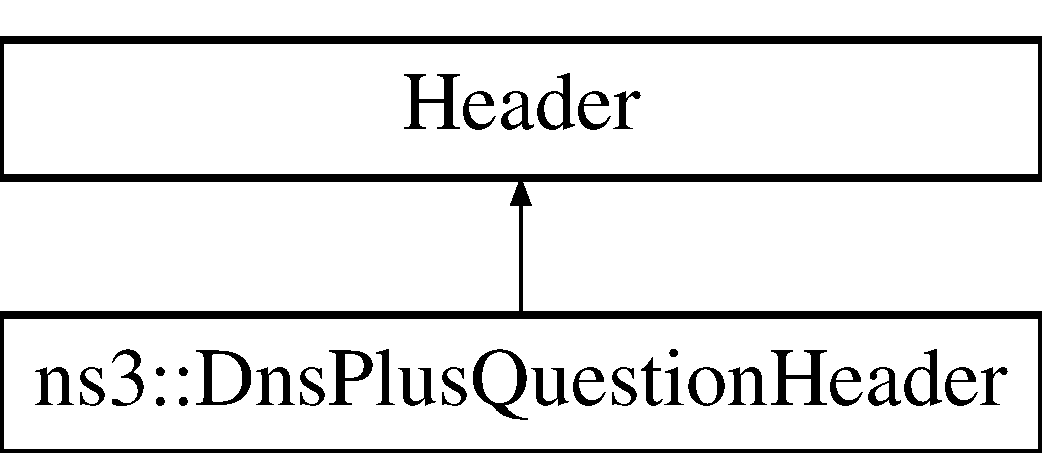
\includegraphics[height=2.000000cm]{classns3_1_1DnsPlusQuestionHeader}
\end{center}
\end{figure}
\subsection*{Public Member Functions}
\begin{DoxyCompactItemize}
\item 
\hyperlink{classns3_1_1DnsPlusQuestionHeader_a3007f16f1486ea4d9e92f0a16304db5c}{Dns\-Plus\-Question\-Header} ()
\item 
virtual \hyperlink{classns3_1_1DnsPlusQuestionHeader_a2491f3d2ea7e19769fe1964405d12da1}{$\sim$\-Dns\-Plus\-Question\-Header} ()
\item 
virtual Type\-Id \hyperlink{classns3_1_1DnsPlusQuestionHeader_a3a22c5fdc183804309a94aad3e09c054}{Get\-Instance\-Type\-Id} (void) const 
\item 
virtual uint32\-\_\-t \hyperlink{classns3_1_1DnsPlusQuestionHeader_a9e90cac30d95e95faaaeeab35fe9c15e}{Get\-Serialized\-Size} (void) const 
\item 
virtual void \hyperlink{classns3_1_1DnsPlusQuestionHeader_a7560e6469a4e5afdf4df095e7e6d6eab}{Serialize} (Buffer\-::\-Iterator start) const 
\item 
virtual uint32\-\_\-t \hyperlink{classns3_1_1DnsPlusQuestionHeader_ac75fc840943cca37028eb0c8a23c4bea}{Deserialize} (Buffer\-::\-Iterator start)
\item 
virtual void \hyperlink{classns3_1_1DnsPlusQuestionHeader_a8ef5f712bae1caef0c7f37590fa094c2}{Print} (std\-::ostream \&os) const 
\item 
void \hyperlink{classns3_1_1DnsPlusQuestionHeader_aaad52033f6142d4c0210fdeb68b95d15}{Set\-Name\-Length} (uint32\-\_\-t name\-Length)
\item 
void \hyperlink{classns3_1_1DnsPlusQuestionHeader_a2fe3d4e1f1eea6817a83e5008d308edf}{Set\-Name} (std\-::string name)
\item 
void \hyperlink{classns3_1_1DnsPlusQuestionHeader_ab4300d1305dfed701fd94d803b5741cd}{Set\-Qtype} (uint16\-\_\-t q\-Type)
\begin{DoxyCompactList}\small\item\em Set the type of data. \end{DoxyCompactList}\item 
void \hyperlink{classns3_1_1DnsPlusQuestionHeader_a8281d02c53d1f3ef5228dd1ddce35759}{Set\-Qclass} (uint16\-\_\-t q\-Class)
\begin{DoxyCompactList}\small\item\em Set the class of data. \end{DoxyCompactList}\item 
void \hyperlink{classns3_1_1DnsPlusQuestionHeader_a7ee32b2fd37340e16532f04670549d70}{Set\-Reserved\-Flag} (uint16\-\_\-t reserved\-Flag)
\begin{DoxyCompactList}\small\item\em Set the Reserved flag, these are not currently used, reserved for future use. \end{DoxyCompactList}\item 
std\-::string \hyperlink{classns3_1_1DnsPlusQuestionHeader_ab999fca8805a988c4917b330594160f5}{Get\-Name} ()
\begin{DoxyCompactList}\small\item\em Get the name of content. \end{DoxyCompactList}\item 
uint16\-\_\-t \hyperlink{classns3_1_1DnsPlusQuestionHeader_a221ec46b8f368cd3e7485bb76a2bbc5a}{Get\-Qclass} ()
\begin{DoxyCompactList}\small\item\em Get the class of the query. \end{DoxyCompactList}\item 
uint16\-\_\-t \hyperlink{classns3_1_1DnsPlusQuestionHeader_a08f7695d808ec124e8a928a5f614b469}{Get\-Qtype} ()
\begin{DoxyCompactList}\small\item\em Get the type of the query. \end{DoxyCompactList}\item 
uint8\-\_\-t \hyperlink{classns3_1_1DnsPlusQuestionHeader_a860734d80f335635c2c80317ec7de319}{Get\-Reserved\-Flag} ()
\begin{DoxyCompactList}\small\item\em Get the reserved flag. \end{DoxyCompactList}\item 
uint32\-\_\-t \hyperlink{classns3_1_1DnsPlusQuestionHeader_a48b9d74d2daecb56ce542b70f196b198}{Get\-Name\-Length} ()
\begin{DoxyCompactList}\small\item\em Get the length of the name. \end{DoxyCompactList}\end{DoxyCompactItemize}
\subsection*{Static Public Member Functions}
\begin{DoxyCompactItemize}
\item 
static Type\-Id \hyperlink{classns3_1_1DnsPlusQuestionHeader_adfca2ccbab64ac86e4e745e761146096}{Get\-Type\-Id} (void)
\begin{DoxyCompactList}\small\item\em Get the type I\-D. \end{DoxyCompactList}\end{DoxyCompactItemize}
\subsection*{Private Attributes}
\begin{DoxyCompactItemize}
\item 
uint8\-\_\-t \hyperlink{classns3_1_1DnsPlusQuestionHeader_a84e44f8fa45c27b13bd7a80ab4d3c648}{m\-\_\-reserved\-Flag}
\begin{DoxyCompactList}\small\item\em reserved flag \end{DoxyCompactList}\item 
std\-::string \hyperlink{classns3_1_1DnsPlusQuestionHeader_a37b7ee88822487ebb7515c4e6d711d9a}{m\-\_\-name}
\begin{DoxyCompactList}\small\item\em name of the content \end{DoxyCompactList}\item 
uint16\-\_\-t \hyperlink{classns3_1_1DnsPlusQuestionHeader_a3bc213161b96f292d6e3d0dab3d42cba}{m\-\_\-q\-Class}
\begin{DoxyCompactList}\small\item\em class of the query \end{DoxyCompactList}\item 
uint16\-\_\-t \hyperlink{classns3_1_1DnsPlusQuestionHeader_a9ec3c28da5e22b33bccb1406ba053876}{m\-\_\-q\-Type}
\begin{DoxyCompactList}\small\item\em type of the query \end{DoxyCompactList}\item 
uint32\-\_\-t \hyperlink{classns3_1_1DnsPlusQuestionHeader_ad17e8994480e0dc6c79ae59a0e4a80c6}{m\-\_\-name\-Length}
\begin{DoxyCompactList}\small\item\em length of the name \end{DoxyCompactList}\end{DoxyCompactItemize}


\subsection{Detailed Description}
It is similar to D\-N\-S Question Section header. It contains the name of the content to be queried. 

\subsection{Constructor \& Destructor Documentation}
\hypertarget{classns3_1_1DnsPlusQuestionHeader_a3007f16f1486ea4d9e92f0a16304db5c}{\index{ns3\-::\-Dns\-Plus\-Question\-Header@{ns3\-::\-Dns\-Plus\-Question\-Header}!Dns\-Plus\-Question\-Header@{Dns\-Plus\-Question\-Header}}
\index{Dns\-Plus\-Question\-Header@{Dns\-Plus\-Question\-Header}!ns3::DnsPlusQuestionHeader@{ns3\-::\-Dns\-Plus\-Question\-Header}}
\subsubsection[{Dns\-Plus\-Question\-Header}]{\setlength{\rightskip}{0pt plus 5cm}ns3\-::\-Dns\-Plus\-Question\-Header\-::\-Dns\-Plus\-Question\-Header (
\begin{DoxyParamCaption}
{}
\end{DoxyParamCaption}
)}}\label{classns3_1_1DnsPlusQuestionHeader_a3007f16f1486ea4d9e92f0a16304db5c}
\hypertarget{classns3_1_1DnsPlusQuestionHeader_a2491f3d2ea7e19769fe1964405d12da1}{\index{ns3\-::\-Dns\-Plus\-Question\-Header@{ns3\-::\-Dns\-Plus\-Question\-Header}!$\sim$\-Dns\-Plus\-Question\-Header@{$\sim$\-Dns\-Plus\-Question\-Header}}
\index{$\sim$\-Dns\-Plus\-Question\-Header@{$\sim$\-Dns\-Plus\-Question\-Header}!ns3::DnsPlusQuestionHeader@{ns3\-::\-Dns\-Plus\-Question\-Header}}
\subsubsection[{$\sim$\-Dns\-Plus\-Question\-Header}]{\setlength{\rightskip}{0pt plus 5cm}ns3\-::\-Dns\-Plus\-Question\-Header\-::$\sim$\-Dns\-Plus\-Question\-Header (
\begin{DoxyParamCaption}
{}
\end{DoxyParamCaption}
)\hspace{0.3cm}{\ttfamily [virtual]}}}\label{classns3_1_1DnsPlusQuestionHeader_a2491f3d2ea7e19769fe1964405d12da1}


\subsection{Member Function Documentation}
\hypertarget{classns3_1_1DnsPlusQuestionHeader_ac75fc840943cca37028eb0c8a23c4bea}{\index{ns3\-::\-Dns\-Plus\-Question\-Header@{ns3\-::\-Dns\-Plus\-Question\-Header}!Deserialize@{Deserialize}}
\index{Deserialize@{Deserialize}!ns3::DnsPlusQuestionHeader@{ns3\-::\-Dns\-Plus\-Question\-Header}}
\subsubsection[{Deserialize}]{\setlength{\rightskip}{0pt plus 5cm}uint32\-\_\-t ns3\-::\-Dns\-Plus\-Question\-Header\-::\-Deserialize (
\begin{DoxyParamCaption}
\item[{Buffer\-::\-Iterator}]{start}
\end{DoxyParamCaption}
)\hspace{0.3cm}{\ttfamily [virtual]}}}\label{classns3_1_1DnsPlusQuestionHeader_ac75fc840943cca37028eb0c8a23c4bea}
\hypertarget{classns3_1_1DnsPlusQuestionHeader_a3a22c5fdc183804309a94aad3e09c054}{\index{ns3\-::\-Dns\-Plus\-Question\-Header@{ns3\-::\-Dns\-Plus\-Question\-Header}!Get\-Instance\-Type\-Id@{Get\-Instance\-Type\-Id}}
\index{Get\-Instance\-Type\-Id@{Get\-Instance\-Type\-Id}!ns3::DnsPlusQuestionHeader@{ns3\-::\-Dns\-Plus\-Question\-Header}}
\subsubsection[{Get\-Instance\-Type\-Id}]{\setlength{\rightskip}{0pt plus 5cm}Type\-Id ns3\-::\-Dns\-Plus\-Question\-Header\-::\-Get\-Instance\-Type\-Id (
\begin{DoxyParamCaption}
\item[{void}]{}
\end{DoxyParamCaption}
) const\hspace{0.3cm}{\ttfamily [virtual]}}}\label{classns3_1_1DnsPlusQuestionHeader_a3a22c5fdc183804309a94aad3e09c054}
\hypertarget{classns3_1_1DnsPlusQuestionHeader_ab999fca8805a988c4917b330594160f5}{\index{ns3\-::\-Dns\-Plus\-Question\-Header@{ns3\-::\-Dns\-Plus\-Question\-Header}!Get\-Name@{Get\-Name}}
\index{Get\-Name@{Get\-Name}!ns3::DnsPlusQuestionHeader@{ns3\-::\-Dns\-Plus\-Question\-Header}}
\subsubsection[{Get\-Name}]{\setlength{\rightskip}{0pt plus 5cm}std\-::string ns3\-::\-Dns\-Plus\-Question\-Header\-::\-Get\-Name (
\begin{DoxyParamCaption}
{}
\end{DoxyParamCaption}
)}}\label{classns3_1_1DnsPlusQuestionHeader_ab999fca8805a988c4917b330594160f5}


Get the name of content. 

\begin{DoxyReturn}{Returns}
name of content. 
\end{DoxyReturn}
\hypertarget{classns3_1_1DnsPlusQuestionHeader_a48b9d74d2daecb56ce542b70f196b198}{\index{ns3\-::\-Dns\-Plus\-Question\-Header@{ns3\-::\-Dns\-Plus\-Question\-Header}!Get\-Name\-Length@{Get\-Name\-Length}}
\index{Get\-Name\-Length@{Get\-Name\-Length}!ns3::DnsPlusQuestionHeader@{ns3\-::\-Dns\-Plus\-Question\-Header}}
\subsubsection[{Get\-Name\-Length}]{\setlength{\rightskip}{0pt plus 5cm}uint32\-\_\-t ns3\-::\-Dns\-Plus\-Question\-Header\-::\-Get\-Name\-Length (
\begin{DoxyParamCaption}
{}
\end{DoxyParamCaption}
)}}\label{classns3_1_1DnsPlusQuestionHeader_a48b9d74d2daecb56ce542b70f196b198}


Get the length of the name. 

\begin{DoxyReturn}{Returns}
length of the name. 
\end{DoxyReturn}
\hypertarget{classns3_1_1DnsPlusQuestionHeader_a221ec46b8f368cd3e7485bb76a2bbc5a}{\index{ns3\-::\-Dns\-Plus\-Question\-Header@{ns3\-::\-Dns\-Plus\-Question\-Header}!Get\-Qclass@{Get\-Qclass}}
\index{Get\-Qclass@{Get\-Qclass}!ns3::DnsPlusQuestionHeader@{ns3\-::\-Dns\-Plus\-Question\-Header}}
\subsubsection[{Get\-Qclass}]{\setlength{\rightskip}{0pt plus 5cm}uint16\-\_\-t ns3\-::\-Dns\-Plus\-Question\-Header\-::\-Get\-Qclass (
\begin{DoxyParamCaption}
{}
\end{DoxyParamCaption}
)}}\label{classns3_1_1DnsPlusQuestionHeader_a221ec46b8f368cd3e7485bb76a2bbc5a}


Get the class of the query. 

\begin{DoxyReturn}{Returns}
class of the query. 
\end{DoxyReturn}
\hypertarget{classns3_1_1DnsPlusQuestionHeader_a08f7695d808ec124e8a928a5f614b469}{\index{ns3\-::\-Dns\-Plus\-Question\-Header@{ns3\-::\-Dns\-Plus\-Question\-Header}!Get\-Qtype@{Get\-Qtype}}
\index{Get\-Qtype@{Get\-Qtype}!ns3::DnsPlusQuestionHeader@{ns3\-::\-Dns\-Plus\-Question\-Header}}
\subsubsection[{Get\-Qtype}]{\setlength{\rightskip}{0pt plus 5cm}uint16\-\_\-t ns3\-::\-Dns\-Plus\-Question\-Header\-::\-Get\-Qtype (
\begin{DoxyParamCaption}
{}
\end{DoxyParamCaption}
)}}\label{classns3_1_1DnsPlusQuestionHeader_a08f7695d808ec124e8a928a5f614b469}


Get the type of the query. 

\begin{DoxyReturn}{Returns}
type of the query. 
\end{DoxyReturn}
\hypertarget{classns3_1_1DnsPlusQuestionHeader_a860734d80f335635c2c80317ec7de319}{\index{ns3\-::\-Dns\-Plus\-Question\-Header@{ns3\-::\-Dns\-Plus\-Question\-Header}!Get\-Reserved\-Flag@{Get\-Reserved\-Flag}}
\index{Get\-Reserved\-Flag@{Get\-Reserved\-Flag}!ns3::DnsPlusQuestionHeader@{ns3\-::\-Dns\-Plus\-Question\-Header}}
\subsubsection[{Get\-Reserved\-Flag}]{\setlength{\rightskip}{0pt plus 5cm}uint8\-\_\-t ns3\-::\-Dns\-Plus\-Question\-Header\-::\-Get\-Reserved\-Flag (
\begin{DoxyParamCaption}
{}
\end{DoxyParamCaption}
)}}\label{classns3_1_1DnsPlusQuestionHeader_a860734d80f335635c2c80317ec7de319}


Get the reserved flag. 

\begin{DoxyReturn}{Returns}
Reserved flag. 
\end{DoxyReturn}
\hypertarget{classns3_1_1DnsPlusQuestionHeader_a9e90cac30d95e95faaaeeab35fe9c15e}{\index{ns3\-::\-Dns\-Plus\-Question\-Header@{ns3\-::\-Dns\-Plus\-Question\-Header}!Get\-Serialized\-Size@{Get\-Serialized\-Size}}
\index{Get\-Serialized\-Size@{Get\-Serialized\-Size}!ns3::DnsPlusQuestionHeader@{ns3\-::\-Dns\-Plus\-Question\-Header}}
\subsubsection[{Get\-Serialized\-Size}]{\setlength{\rightskip}{0pt plus 5cm}uint32\-\_\-t ns3\-::\-Dns\-Plus\-Question\-Header\-::\-Get\-Serialized\-Size (
\begin{DoxyParamCaption}
\item[{void}]{}
\end{DoxyParamCaption}
) const\hspace{0.3cm}{\ttfamily [virtual]}}}\label{classns3_1_1DnsPlusQuestionHeader_a9e90cac30d95e95faaaeeab35fe9c15e}
\hypertarget{classns3_1_1DnsPlusQuestionHeader_adfca2ccbab64ac86e4e745e761146096}{\index{ns3\-::\-Dns\-Plus\-Question\-Header@{ns3\-::\-Dns\-Plus\-Question\-Header}!Get\-Type\-Id@{Get\-Type\-Id}}
\index{Get\-Type\-Id@{Get\-Type\-Id}!ns3::DnsPlusQuestionHeader@{ns3\-::\-Dns\-Plus\-Question\-Header}}
\subsubsection[{Get\-Type\-Id}]{\setlength{\rightskip}{0pt plus 5cm}Type\-Id ns3\-::\-Dns\-Plus\-Question\-Header\-::\-Get\-Type\-Id (
\begin{DoxyParamCaption}
\item[{void}]{}
\end{DoxyParamCaption}
)\hspace{0.3cm}{\ttfamily [static]}}}\label{classns3_1_1DnsPlusQuestionHeader_adfca2ccbab64ac86e4e745e761146096}


Get the type I\-D. 

\begin{DoxyReturn}{Returns}
the object Type\-Id. 
\end{DoxyReturn}
\hypertarget{classns3_1_1DnsPlusQuestionHeader_a8ef5f712bae1caef0c7f37590fa094c2}{\index{ns3\-::\-Dns\-Plus\-Question\-Header@{ns3\-::\-Dns\-Plus\-Question\-Header}!Print@{Print}}
\index{Print@{Print}!ns3::DnsPlusQuestionHeader@{ns3\-::\-Dns\-Plus\-Question\-Header}}
\subsubsection[{Print}]{\setlength{\rightskip}{0pt plus 5cm}void ns3\-::\-Dns\-Plus\-Question\-Header\-::\-Print (
\begin{DoxyParamCaption}
\item[{std\-::ostream \&}]{os}
\end{DoxyParamCaption}
) const\hspace{0.3cm}{\ttfamily [virtual]}}}\label{classns3_1_1DnsPlusQuestionHeader_a8ef5f712bae1caef0c7f37590fa094c2}
\hypertarget{classns3_1_1DnsPlusQuestionHeader_a7560e6469a4e5afdf4df095e7e6d6eab}{\index{ns3\-::\-Dns\-Plus\-Question\-Header@{ns3\-::\-Dns\-Plus\-Question\-Header}!Serialize@{Serialize}}
\index{Serialize@{Serialize}!ns3::DnsPlusQuestionHeader@{ns3\-::\-Dns\-Plus\-Question\-Header}}
\subsubsection[{Serialize}]{\setlength{\rightskip}{0pt plus 5cm}void ns3\-::\-Dns\-Plus\-Question\-Header\-::\-Serialize (
\begin{DoxyParamCaption}
\item[{Buffer\-::\-Iterator}]{start}
\end{DoxyParamCaption}
) const\hspace{0.3cm}{\ttfamily [virtual]}}}\label{classns3_1_1DnsPlusQuestionHeader_a7560e6469a4e5afdf4df095e7e6d6eab}
\hypertarget{classns3_1_1DnsPlusQuestionHeader_a2fe3d4e1f1eea6817a83e5008d308edf}{\index{ns3\-::\-Dns\-Plus\-Question\-Header@{ns3\-::\-Dns\-Plus\-Question\-Header}!Set\-Name@{Set\-Name}}
\index{Set\-Name@{Set\-Name}!ns3::DnsPlusQuestionHeader@{ns3\-::\-Dns\-Plus\-Question\-Header}}
\subsubsection[{Set\-Name}]{\setlength{\rightskip}{0pt plus 5cm}void ns3\-::\-Dns\-Plus\-Question\-Header\-::\-Set\-Name (
\begin{DoxyParamCaption}
\item[{std\-::string}]{name}
\end{DoxyParamCaption}
)}}\label{classns3_1_1DnsPlusQuestionHeader_a2fe3d4e1f1eea6817a83e5008d308edf}
Set the name of the content. 
\begin{DoxyParams}{Parameters}
{\em name} & name of the content. \\
\hline
\end{DoxyParams}
\hypertarget{classns3_1_1DnsPlusQuestionHeader_aaad52033f6142d4c0210fdeb68b95d15}{\index{ns3\-::\-Dns\-Plus\-Question\-Header@{ns3\-::\-Dns\-Plus\-Question\-Header}!Set\-Name\-Length@{Set\-Name\-Length}}
\index{Set\-Name\-Length@{Set\-Name\-Length}!ns3::DnsPlusQuestionHeader@{ns3\-::\-Dns\-Plus\-Question\-Header}}
\subsubsection[{Set\-Name\-Length}]{\setlength{\rightskip}{0pt plus 5cm}void ns3\-::\-Dns\-Plus\-Question\-Header\-::\-Set\-Name\-Length (
\begin{DoxyParamCaption}
\item[{uint32\-\_\-t}]{name\-Length}
\end{DoxyParamCaption}
)}}\label{classns3_1_1DnsPlusQuestionHeader_aaad52033f6142d4c0210fdeb68b95d15}
Set the length of the name. 
\begin{DoxyParams}{Parameters}
{\em name\-Length} & length of the name. \\
\hline
\end{DoxyParams}
\hypertarget{classns3_1_1DnsPlusQuestionHeader_a8281d02c53d1f3ef5228dd1ddce35759}{\index{ns3\-::\-Dns\-Plus\-Question\-Header@{ns3\-::\-Dns\-Plus\-Question\-Header}!Set\-Qclass@{Set\-Qclass}}
\index{Set\-Qclass@{Set\-Qclass}!ns3::DnsPlusQuestionHeader@{ns3\-::\-Dns\-Plus\-Question\-Header}}
\subsubsection[{Set\-Qclass}]{\setlength{\rightskip}{0pt plus 5cm}void ns3\-::\-Dns\-Plus\-Question\-Header\-::\-Set\-Qclass (
\begin{DoxyParamCaption}
\item[{uint16\-\_\-t}]{q\-Class}
\end{DoxyParamCaption}
)}}\label{classns3_1_1DnsPlusQuestionHeader_a8281d02c53d1f3ef5228dd1ddce35759}


Set the class of data. 


\begin{DoxyParams}{Parameters}
{\em q\-Class} & class of data. \\
\hline
\end{DoxyParams}
\hypertarget{classns3_1_1DnsPlusQuestionHeader_ab4300d1305dfed701fd94d803b5741cd}{\index{ns3\-::\-Dns\-Plus\-Question\-Header@{ns3\-::\-Dns\-Plus\-Question\-Header}!Set\-Qtype@{Set\-Qtype}}
\index{Set\-Qtype@{Set\-Qtype}!ns3::DnsPlusQuestionHeader@{ns3\-::\-Dns\-Plus\-Question\-Header}}
\subsubsection[{Set\-Qtype}]{\setlength{\rightskip}{0pt plus 5cm}void ns3\-::\-Dns\-Plus\-Question\-Header\-::\-Set\-Qtype (
\begin{DoxyParamCaption}
\item[{uint16\-\_\-t}]{q\-Type}
\end{DoxyParamCaption}
)}}\label{classns3_1_1DnsPlusQuestionHeader_ab4300d1305dfed701fd94d803b5741cd}


Set the type of data. 


\begin{DoxyParams}{Parameters}
{\em q\-Type} & type of data. \\
\hline
\end{DoxyParams}
\hypertarget{classns3_1_1DnsPlusQuestionHeader_a7ee32b2fd37340e16532f04670549d70}{\index{ns3\-::\-Dns\-Plus\-Question\-Header@{ns3\-::\-Dns\-Plus\-Question\-Header}!Set\-Reserved\-Flag@{Set\-Reserved\-Flag}}
\index{Set\-Reserved\-Flag@{Set\-Reserved\-Flag}!ns3::DnsPlusQuestionHeader@{ns3\-::\-Dns\-Plus\-Question\-Header}}
\subsubsection[{Set\-Reserved\-Flag}]{\setlength{\rightskip}{0pt plus 5cm}void ns3\-::\-Dns\-Plus\-Question\-Header\-::\-Set\-Reserved\-Flag (
\begin{DoxyParamCaption}
\item[{uint16\-\_\-t}]{reserved\-Flag}
\end{DoxyParamCaption}
)}}\label{classns3_1_1DnsPlusQuestionHeader_a7ee32b2fd37340e16532f04670549d70}


Set the Reserved flag, these are not currently used, reserved for future use. 


\begin{DoxyParams}{Parameters}
{\em reserved\-Flag} & reserved flag bit. \\
\hline
\end{DoxyParams}


\subsection{Member Data Documentation}
\hypertarget{classns3_1_1DnsPlusQuestionHeader_a37b7ee88822487ebb7515c4e6d711d9a}{\index{ns3\-::\-Dns\-Plus\-Question\-Header@{ns3\-::\-Dns\-Plus\-Question\-Header}!m\-\_\-name@{m\-\_\-name}}
\index{m\-\_\-name@{m\-\_\-name}!ns3::DnsPlusQuestionHeader@{ns3\-::\-Dns\-Plus\-Question\-Header}}
\subsubsection[{m\-\_\-name}]{\setlength{\rightskip}{0pt plus 5cm}std\-::string ns3\-::\-Dns\-Plus\-Question\-Header\-::m\-\_\-name\hspace{0.3cm}{\ttfamily [private]}}}\label{classns3_1_1DnsPlusQuestionHeader_a37b7ee88822487ebb7515c4e6d711d9a}


name of the content 

\hypertarget{classns3_1_1DnsPlusQuestionHeader_ad17e8994480e0dc6c79ae59a0e4a80c6}{\index{ns3\-::\-Dns\-Plus\-Question\-Header@{ns3\-::\-Dns\-Plus\-Question\-Header}!m\-\_\-name\-Length@{m\-\_\-name\-Length}}
\index{m\-\_\-name\-Length@{m\-\_\-name\-Length}!ns3::DnsPlusQuestionHeader@{ns3\-::\-Dns\-Plus\-Question\-Header}}
\subsubsection[{m\-\_\-name\-Length}]{\setlength{\rightskip}{0pt plus 5cm}uint32\-\_\-t ns3\-::\-Dns\-Plus\-Question\-Header\-::m\-\_\-name\-Length\hspace{0.3cm}{\ttfamily [private]}}}\label{classns3_1_1DnsPlusQuestionHeader_ad17e8994480e0dc6c79ae59a0e4a80c6}


length of the name 

\hypertarget{classns3_1_1DnsPlusQuestionHeader_a3bc213161b96f292d6e3d0dab3d42cba}{\index{ns3\-::\-Dns\-Plus\-Question\-Header@{ns3\-::\-Dns\-Plus\-Question\-Header}!m\-\_\-q\-Class@{m\-\_\-q\-Class}}
\index{m\-\_\-q\-Class@{m\-\_\-q\-Class}!ns3::DnsPlusQuestionHeader@{ns3\-::\-Dns\-Plus\-Question\-Header}}
\subsubsection[{m\-\_\-q\-Class}]{\setlength{\rightskip}{0pt plus 5cm}uint16\-\_\-t ns3\-::\-Dns\-Plus\-Question\-Header\-::m\-\_\-q\-Class\hspace{0.3cm}{\ttfamily [private]}}}\label{classns3_1_1DnsPlusQuestionHeader_a3bc213161b96f292d6e3d0dab3d42cba}


class of the query 

\hypertarget{classns3_1_1DnsPlusQuestionHeader_a9ec3c28da5e22b33bccb1406ba053876}{\index{ns3\-::\-Dns\-Plus\-Question\-Header@{ns3\-::\-Dns\-Plus\-Question\-Header}!m\-\_\-q\-Type@{m\-\_\-q\-Type}}
\index{m\-\_\-q\-Type@{m\-\_\-q\-Type}!ns3::DnsPlusQuestionHeader@{ns3\-::\-Dns\-Plus\-Question\-Header}}
\subsubsection[{m\-\_\-q\-Type}]{\setlength{\rightskip}{0pt plus 5cm}uint16\-\_\-t ns3\-::\-Dns\-Plus\-Question\-Header\-::m\-\_\-q\-Type\hspace{0.3cm}{\ttfamily [private]}}}\label{classns3_1_1DnsPlusQuestionHeader_a9ec3c28da5e22b33bccb1406ba053876}


type of the query 

\hypertarget{classns3_1_1DnsPlusQuestionHeader_a84e44f8fa45c27b13bd7a80ab4d3c648}{\index{ns3\-::\-Dns\-Plus\-Question\-Header@{ns3\-::\-Dns\-Plus\-Question\-Header}!m\-\_\-reserved\-Flag@{m\-\_\-reserved\-Flag}}
\index{m\-\_\-reserved\-Flag@{m\-\_\-reserved\-Flag}!ns3::DnsPlusQuestionHeader@{ns3\-::\-Dns\-Plus\-Question\-Header}}
\subsubsection[{m\-\_\-reserved\-Flag}]{\setlength{\rightskip}{0pt plus 5cm}uint8\-\_\-t ns3\-::\-Dns\-Plus\-Question\-Header\-::m\-\_\-reserved\-Flag\hspace{0.3cm}{\ttfamily [private]}}}\label{classns3_1_1DnsPlusQuestionHeader_a84e44f8fa45c27b13bd7a80ab4d3c648}


reserved flag 



The documentation for this class was generated from the following files\-:\begin{DoxyCompactItemize}
\item 
model/\hyperlink{dnsplus-question-header_8h}{dnsplus-\/question-\/header.\-h}\item 
model/\hyperlink{dnsplus-question-header_8cc}{dnsplus-\/question-\/header.\-cc}\end{DoxyCompactItemize}

\hypertarget{classns3_1_1Ipv4RouterL3Protocol_1_1Fragments}{\section{ns3\-:\-:Ipv4\-Router\-L3\-Protocol\-:\-:Fragments Class Reference}
\label{classns3_1_1Ipv4RouterL3Protocol_1_1Fragments}\index{ns3\-::\-Ipv4\-Router\-L3\-Protocol\-::\-Fragments@{ns3\-::\-Ipv4\-Router\-L3\-Protocol\-::\-Fragments}}
}


A Set of Fragment belonging to the same packet (src, dst, identification and proto)  


Inheritance diagram for ns3\-:\-:Ipv4\-Router\-L3\-Protocol\-:\-:Fragments\-:\begin{figure}[H]
\begin{center}
\leavevmode
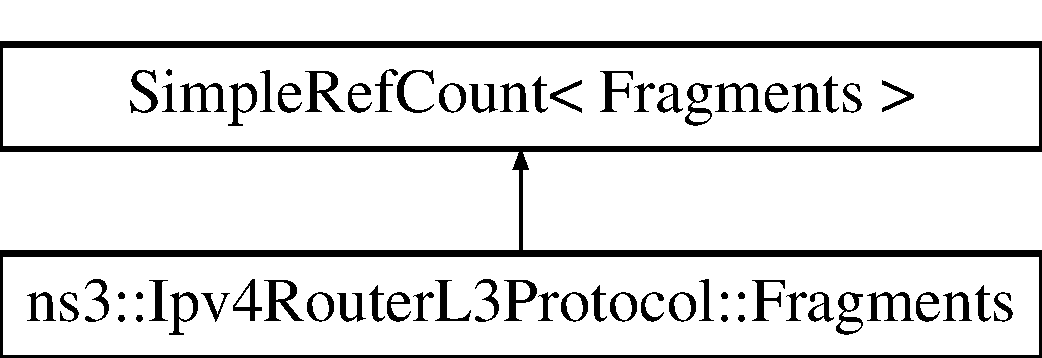
\includegraphics[height=2.000000cm]{classns3_1_1Ipv4RouterL3Protocol_1_1Fragments}
\end{center}
\end{figure}
\subsection*{Public Member Functions}
\begin{DoxyCompactItemize}
\item 
\hyperlink{classns3_1_1Ipv4RouterL3Protocol_1_1Fragments_a79843dcefae495214fd0409216c752bb}{Fragments} ()
\begin{DoxyCompactList}\small\item\em Constructor. \end{DoxyCompactList}\item 
\hyperlink{classns3_1_1Ipv4RouterL3Protocol_1_1Fragments_aaef0bfaf9061b6a19f27a438fc20f3ae}{$\sim$\-Fragments} ()
\begin{DoxyCompactList}\small\item\em Destructor. \end{DoxyCompactList}\item 
void \hyperlink{classns3_1_1Ipv4RouterL3Protocol_1_1Fragments_a5d4cc40fc1ba11c52024f674bdc1ddb7}{Add\-Fragment} (Ptr$<$ Packet $>$ fragment, uint16\-\_\-t fragment\-Offset, bool more\-Fragment)
\begin{DoxyCompactList}\small\item\em Add a fragment. \end{DoxyCompactList}\item 
bool \hyperlink{classns3_1_1Ipv4RouterL3Protocol_1_1Fragments_a1800010de516168a088838f33d7ad1c7}{Is\-Entire} () const 
\begin{DoxyCompactList}\small\item\em If all fragments have been added. \end{DoxyCompactList}\item 
Ptr$<$ Packet $>$ \hyperlink{classns3_1_1Ipv4RouterL3Protocol_1_1Fragments_a6d46b37853fb6275e7ee17cc011df935}{Get\-Packet} () const 
\begin{DoxyCompactList}\small\item\em Get the entire packet. \end{DoxyCompactList}\item 
Ptr$<$ Packet $>$ \hyperlink{classns3_1_1Ipv4RouterL3Protocol_1_1Fragments_a66b105030585bb6e71cffd8a4990a510}{Get\-Partial\-Packet} () const 
\begin{DoxyCompactList}\small\item\em Get the complete part of the packet. \end{DoxyCompactList}\end{DoxyCompactItemize}
\subsection*{Private Attributes}
\begin{DoxyCompactItemize}
\item 
bool \hyperlink{classns3_1_1Ipv4RouterL3Protocol_1_1Fragments_a98acf0bddf84056bce2281fe62669cd1}{m\-\_\-more\-Fragment}
\begin{DoxyCompactList}\small\item\em True if other fragments will be sent. \end{DoxyCompactList}\item 
std\-::list$<$ std\-::pair$<$ Ptr\\*
$<$ Packet $>$, uint16\-\_\-t $>$ $>$ \hyperlink{classns3_1_1Ipv4RouterL3Protocol_1_1Fragments_abdb3e0b06a2799f3bef00330ea0d66a2}{m\-\_\-fragments}
\begin{DoxyCompactList}\small\item\em The current fragments. \end{DoxyCompactList}\end{DoxyCompactItemize}


\subsection{Detailed Description}
A Set of Fragment belonging to the same packet (src, dst, identification and proto) 

\subsection{Constructor \& Destructor Documentation}
\hypertarget{classns3_1_1Ipv4RouterL3Protocol_1_1Fragments_a79843dcefae495214fd0409216c752bb}{\index{ns3\-::\-Ipv4\-Router\-L3\-Protocol\-::\-Fragments@{ns3\-::\-Ipv4\-Router\-L3\-Protocol\-::\-Fragments}!Fragments@{Fragments}}
\index{Fragments@{Fragments}!ns3::Ipv4RouterL3Protocol::Fragments@{ns3\-::\-Ipv4\-Router\-L3\-Protocol\-::\-Fragments}}
\subsubsection[{Fragments}]{\setlength{\rightskip}{0pt plus 5cm}ns3\-::\-Ipv4\-Router\-L3\-Protocol\-::\-Fragments\-::\-Fragments (
\begin{DoxyParamCaption}
{}
\end{DoxyParamCaption}
)}}\label{classns3_1_1Ipv4RouterL3Protocol_1_1Fragments_a79843dcefae495214fd0409216c752bb}


Constructor. 

\hypertarget{classns3_1_1Ipv4RouterL3Protocol_1_1Fragments_aaef0bfaf9061b6a19f27a438fc20f3ae}{\index{ns3\-::\-Ipv4\-Router\-L3\-Protocol\-::\-Fragments@{ns3\-::\-Ipv4\-Router\-L3\-Protocol\-::\-Fragments}!$\sim$\-Fragments@{$\sim$\-Fragments}}
\index{$\sim$\-Fragments@{$\sim$\-Fragments}!ns3::Ipv4RouterL3Protocol::Fragments@{ns3\-::\-Ipv4\-Router\-L3\-Protocol\-::\-Fragments}}
\subsubsection[{$\sim$\-Fragments}]{\setlength{\rightskip}{0pt plus 5cm}ns3\-::\-Ipv4\-Router\-L3\-Protocol\-::\-Fragments\-::$\sim$\-Fragments (
\begin{DoxyParamCaption}
{}
\end{DoxyParamCaption}
)}}\label{classns3_1_1Ipv4RouterL3Protocol_1_1Fragments_aaef0bfaf9061b6a19f27a438fc20f3ae}


Destructor. 



\subsection{Member Function Documentation}
\hypertarget{classns3_1_1Ipv4RouterL3Protocol_1_1Fragments_a5d4cc40fc1ba11c52024f674bdc1ddb7}{\index{ns3\-::\-Ipv4\-Router\-L3\-Protocol\-::\-Fragments@{ns3\-::\-Ipv4\-Router\-L3\-Protocol\-::\-Fragments}!Add\-Fragment@{Add\-Fragment}}
\index{Add\-Fragment@{Add\-Fragment}!ns3::Ipv4RouterL3Protocol::Fragments@{ns3\-::\-Ipv4\-Router\-L3\-Protocol\-::\-Fragments}}
\subsubsection[{Add\-Fragment}]{\setlength{\rightskip}{0pt plus 5cm}void ns3\-::\-Ipv4\-Router\-L3\-Protocol\-::\-Fragments\-::\-Add\-Fragment (
\begin{DoxyParamCaption}
\item[{Ptr$<$ Packet $>$}]{fragment, }
\item[{uint16\-\_\-t}]{fragment\-Offset, }
\item[{bool}]{more\-Fragment}
\end{DoxyParamCaption}
)}}\label{classns3_1_1Ipv4RouterL3Protocol_1_1Fragments_a5d4cc40fc1ba11c52024f674bdc1ddb7}


Add a fragment. 


\begin{DoxyParams}{Parameters}
{\em fragment} & the fragment \\
\hline
{\em fragment\-Offset} & the offset of the fragment \\
\hline
{\em more\-Fragment} & the bit \char`\"{}\-More Fragment\char`\"{} \\
\hline
\end{DoxyParams}
\hypertarget{classns3_1_1Ipv4RouterL3Protocol_1_1Fragments_a6d46b37853fb6275e7ee17cc011df935}{\index{ns3\-::\-Ipv4\-Router\-L3\-Protocol\-::\-Fragments@{ns3\-::\-Ipv4\-Router\-L3\-Protocol\-::\-Fragments}!Get\-Packet@{Get\-Packet}}
\index{Get\-Packet@{Get\-Packet}!ns3::Ipv4RouterL3Protocol::Fragments@{ns3\-::\-Ipv4\-Router\-L3\-Protocol\-::\-Fragments}}
\subsubsection[{Get\-Packet}]{\setlength{\rightskip}{0pt plus 5cm}Ptr$<$ Packet $>$ ns3\-::\-Ipv4\-Router\-L3\-Protocol\-::\-Fragments\-::\-Get\-Packet (
\begin{DoxyParamCaption}
{}
\end{DoxyParamCaption}
) const}}\label{classns3_1_1Ipv4RouterL3Protocol_1_1Fragments_a6d46b37853fb6275e7ee17cc011df935}


Get the entire packet. 

\begin{DoxyReturn}{Returns}
the entire packet 
\end{DoxyReturn}
\hypertarget{classns3_1_1Ipv4RouterL3Protocol_1_1Fragments_a66b105030585bb6e71cffd8a4990a510}{\index{ns3\-::\-Ipv4\-Router\-L3\-Protocol\-::\-Fragments@{ns3\-::\-Ipv4\-Router\-L3\-Protocol\-::\-Fragments}!Get\-Partial\-Packet@{Get\-Partial\-Packet}}
\index{Get\-Partial\-Packet@{Get\-Partial\-Packet}!ns3::Ipv4RouterL3Protocol::Fragments@{ns3\-::\-Ipv4\-Router\-L3\-Protocol\-::\-Fragments}}
\subsubsection[{Get\-Partial\-Packet}]{\setlength{\rightskip}{0pt plus 5cm}Ptr$<$ Packet $>$ ns3\-::\-Ipv4\-Router\-L3\-Protocol\-::\-Fragments\-::\-Get\-Partial\-Packet (
\begin{DoxyParamCaption}
{}
\end{DoxyParamCaption}
) const}}\label{classns3_1_1Ipv4RouterL3Protocol_1_1Fragments_a66b105030585bb6e71cffd8a4990a510}


Get the complete part of the packet. 

\begin{DoxyReturn}{Returns}
the part we have comeplete 
\end{DoxyReturn}
\hypertarget{classns3_1_1Ipv4RouterL3Protocol_1_1Fragments_a1800010de516168a088838f33d7ad1c7}{\index{ns3\-::\-Ipv4\-Router\-L3\-Protocol\-::\-Fragments@{ns3\-::\-Ipv4\-Router\-L3\-Protocol\-::\-Fragments}!Is\-Entire@{Is\-Entire}}
\index{Is\-Entire@{Is\-Entire}!ns3::Ipv4RouterL3Protocol::Fragments@{ns3\-::\-Ipv4\-Router\-L3\-Protocol\-::\-Fragments}}
\subsubsection[{Is\-Entire}]{\setlength{\rightskip}{0pt plus 5cm}bool ns3\-::\-Ipv4\-Router\-L3\-Protocol\-::\-Fragments\-::\-Is\-Entire (
\begin{DoxyParamCaption}
{}
\end{DoxyParamCaption}
) const}}\label{classns3_1_1Ipv4RouterL3Protocol_1_1Fragments_a1800010de516168a088838f33d7ad1c7}


If all fragments have been added. 

\begin{DoxyReturn}{Returns}
true if the packet is entire 
\end{DoxyReturn}


\subsection{Member Data Documentation}
\hypertarget{classns3_1_1Ipv4RouterL3Protocol_1_1Fragments_abdb3e0b06a2799f3bef00330ea0d66a2}{\index{ns3\-::\-Ipv4\-Router\-L3\-Protocol\-::\-Fragments@{ns3\-::\-Ipv4\-Router\-L3\-Protocol\-::\-Fragments}!m\-\_\-fragments@{m\-\_\-fragments}}
\index{m\-\_\-fragments@{m\-\_\-fragments}!ns3::Ipv4RouterL3Protocol::Fragments@{ns3\-::\-Ipv4\-Router\-L3\-Protocol\-::\-Fragments}}
\subsubsection[{m\-\_\-fragments}]{\setlength{\rightskip}{0pt plus 5cm}std\-::list$<$std\-::pair$<$Ptr$<$Packet$>$, uint16\-\_\-t$>$ $>$ ns3\-::\-Ipv4\-Router\-L3\-Protocol\-::\-Fragments\-::m\-\_\-fragments\hspace{0.3cm}{\ttfamily [private]}}}\label{classns3_1_1Ipv4RouterL3Protocol_1_1Fragments_abdb3e0b06a2799f3bef00330ea0d66a2}


The current fragments. 

\hypertarget{classns3_1_1Ipv4RouterL3Protocol_1_1Fragments_a98acf0bddf84056bce2281fe62669cd1}{\index{ns3\-::\-Ipv4\-Router\-L3\-Protocol\-::\-Fragments@{ns3\-::\-Ipv4\-Router\-L3\-Protocol\-::\-Fragments}!m\-\_\-more\-Fragment@{m\-\_\-more\-Fragment}}
\index{m\-\_\-more\-Fragment@{m\-\_\-more\-Fragment}!ns3::Ipv4RouterL3Protocol::Fragments@{ns3\-::\-Ipv4\-Router\-L3\-Protocol\-::\-Fragments}}
\subsubsection[{m\-\_\-more\-Fragment}]{\setlength{\rightskip}{0pt plus 5cm}bool ns3\-::\-Ipv4\-Router\-L3\-Protocol\-::\-Fragments\-::m\-\_\-more\-Fragment\hspace{0.3cm}{\ttfamily [private]}}}\label{classns3_1_1Ipv4RouterL3Protocol_1_1Fragments_a98acf0bddf84056bce2281fe62669cd1}


True if other fragments will be sent. 



The documentation for this class was generated from the following files\-:\begin{DoxyCompactItemize}
\item 
model/\hyperlink{ipv4-router-l3-protocol_8h}{ipv4-\/router-\/l3-\/protocol.\-h}\item 
model/\hyperlink{ipv4-router-l3-protocol_8cc}{ipv4-\/router-\/l3-\/protocol.\-cc}\end{DoxyCompactItemize}

\hypertarget{classns3_1_1IcnManager}{\section{ns3\-:\-:Icn\-Manager Class Reference}
\label{classns3_1_1IcnManager}\index{ns3\-::\-Icn\-Manager@{ns3\-::\-Icn\-Manager}}
}


It resolves the name requested by the client and direct the source (server or cached source(router)) to send the requested content back to client.  




{\ttfamily \#include $<$icn-\/manager.\-h$>$}

Inheritance diagram for ns3\-:\-:Icn\-Manager\-:\begin{figure}[H]
\begin{center}
\leavevmode
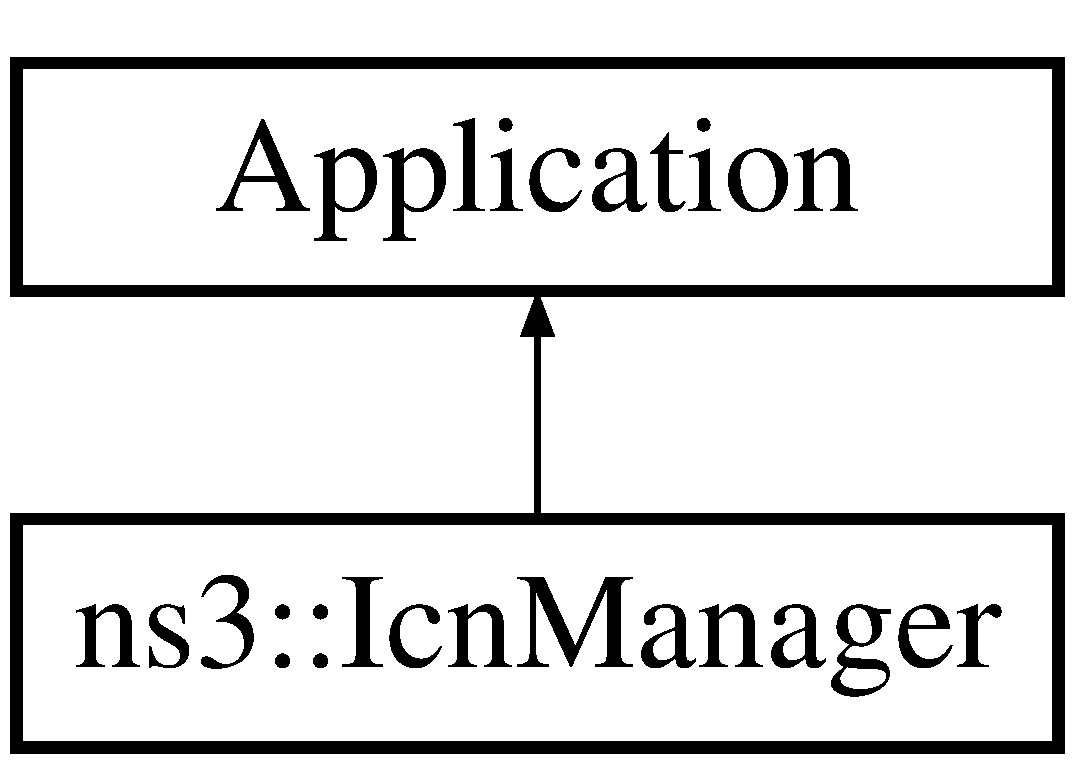
\includegraphics[height=2.000000cm]{classns3_1_1IcnManager}
\end{center}
\end{figure}
\subsection*{Public Member Functions}
\begin{DoxyCompactItemize}
\item 
\hyperlink{classns3_1_1IcnManager_a1f48e87348770a7857f1dbbf4279b169}{Icn\-Manager} ()
\item 
void \hyperlink{classns3_1_1IcnManager_af448a19c4cbb801cc0e794a680c95e7a}{Read\-Packet} (Ptr$<$ Packet $>$ packet, Ipv4\-Address client\-Address, uint16\-\_\-t client\-Port)
\begin{DoxyCompactList}\small\item\em Read the packet received. If packet received is content query packet from O\-I\-C\-N Client, it call Name\-Resolution function to know the source of the content. Further if name resolution is successful, it sends A\-C\-K to client, otherwise it sends N\-A\-C\-K to client. \end{DoxyCompactList}\item 
Ipv4\-Address const $\ast$ \hyperlink{classns3_1_1IcnManager_a305b143330eaf36bba91e86eba4619fd}{Name\-Resolution} (std\-::string name, bool \&flag)
\begin{DoxyCompactList}\small\item\em Search the name in Cached\-Router\-Table or name\-Server\-Table. \end{DoxyCompactList}\item 
void \hyperlink{classns3_1_1IcnManager_acc48cc930981a8e45d440559139b9c1f}{Name\-Registeration} (std\-::vector$<$ std\-::vector$<$ int $>$$>$ name\-Index, std\-::vector$<$ Ipv4\-Address $>$ server\-Address)
\begin{DoxyCompactList}\small\item\em Initialise name\-Server\-Table with name and corresponding server ipv4 address. \end{DoxyCompactList}\item 
void \hyperlink{classns3_1_1IcnManager_a7152eb46e71b0e33cbb6ccd23cbe6266}{Send\-Ack\-To\-Client} (Ipv4\-Address client\-Ipv4\-Address, uint16\-\_\-t client\-Port, \hyperlink{classns3_1_1DnsPlusQuestionHeader}{Dns\-Plus\-Question\-Header} dns\-Plus\-Question\-Header, \hyperlink{classns3_1_1DnsPlusHeader}{Dns\-Plus\-Header} dns\-Plus\-Header, \hyperlink{classns3_1_1OicnHeader}{Oicn\-Header} oicn\-Header, bool \&flag)
\begin{DoxyCompactList}\small\item\em Send A\-C\-K/\-N\-A\-C\-K to client depending upon I\-C\-N Manager has able to resolve name or not. \end{DoxyCompactList}\item 
void \hyperlink{classns3_1_1IcnManager_af503cd858bfb757c2eb55b25876d9cb2}{Send\-To\-Source} (Ipv4\-Address source\-Ip\-Address, Ipv4\-Address client\-Ipv4\-Address, \hyperlink{classns3_1_1DnsPlusQuestionHeader}{Dns\-Plus\-Question\-Header} dns\-Plus\-Question\-Header, \hyperlink{classns3_1_1DnsPlusHeader}{Dns\-Plus\-Header} dns\-Plus\-Header, \hyperlink{classns3_1_1OicnHeader}{Oicn\-Header} oicn\-Header)
\begin{DoxyCompactList}\small\item\em Send Reply packet (with dns\-Plus Answer section) to source of content. dns\-Plus Answer section contains client ipv4 address. It directs the source of content to send the content at mentioned client address. \end{DoxyCompactList}\end{DoxyCompactItemize}
\subsection*{Static Public Member Functions}
\begin{DoxyCompactItemize}
\item 
static Type\-Id \hyperlink{classns3_1_1IcnManager_afbbd24928df50c3489f381f1848dddf1}{Get\-Type\-Id} (void)
\begin{DoxyCompactList}\small\item\em Get the type I\-D. \end{DoxyCompactList}\item 
static void \hyperlink{classns3_1_1IcnManager_a799aa85b5dbecb91214d0e6c52fc697c}{Set\-Cached\-Router\-Entry} (Ipv4\-Address router\-Ipv4\-Address, std\-::string name)
\begin{DoxyCompactList}\small\item\em Enter the name of the content and ipv4 address of corresponding router into Cached\-Router\-Table. \end{DoxyCompactList}\item 
static void \hyperlink{classns3_1_1IcnManager_a61f9b8234e2f57bcc5d4d410423dfda6}{Evict\-Cached\-Router\-Entry} (Ipv4\-Address router\-Ipv4\-Address, std\-::string name)
\begin{DoxyCompactList}\small\item\em Evict the name of the content and ipv4 address of corresponding router from Cached\-Router\-Table. \end{DoxyCompactList}\end{DoxyCompactItemize}
\subsection*{Protected Member Functions}
\begin{DoxyCompactItemize}
\item 
virtual void \hyperlink{classns3_1_1IcnManager_ad7e1a50c5d1411ae7e73a489be9c1503}{Do\-Dispose} (void)
\end{DoxyCompactItemize}
\subsection*{Private Member Functions}
\begin{DoxyCompactItemize}
\item 
void \hyperlink{classns3_1_1IcnManager_a34f69ccb754cb9d10f1020d1058e49fa}{Handle\-Read\-Client} (Ptr$<$ Socket $>$ socket)
\begin{DoxyCompactList}\small\item\em Handle a packet reception from client port (26). This function is called by lower layers. \end{DoxyCompactList}\item 
void \hyperlink{classns3_1_1IcnManager_aa22b16c46e5f98443973564a875a6f58}{Handle\-Read\-Source} (Ptr$<$ Socket $>$ socket)
\begin{DoxyCompactList}\small\item\em Handle a packet reception from source port (both server source and cached source(icn router) port 89). This function is called by lower layers. \end{DoxyCompactList}\item 
virtual void \hyperlink{classns3_1_1IcnManager_ab65232c50cfdee86da1edbe3bb92c644}{Start\-Application} (void)
\item 
virtual void \hyperlink{classns3_1_1IcnManager_a609f7f582c1ffe00d45fd1ce3dbf27f2}{Stop\-Application} (void)
\end{DoxyCompactItemize}
\subsection*{Private Attributes}
\begin{DoxyCompactItemize}
\item 
uint32\-\_\-t \hyperlink{classns3_1_1IcnManager_a43c8815cc7e2746f7c96e8e847ee6c03}{m\-\_\-count}
\begin{DoxyCompactList}\small\item\em maximum number of packets the application will send \end{DoxyCompactList}\item 
Time \hyperlink{classns3_1_1IcnManager_a4064521e1b0c672c5cf34ae49a7a97c7}{m\-\_\-interval}
\begin{DoxyCompactList}\small\item\em packet inter-\/send time \end{DoxyCompactList}\item 
uint32\-\_\-t \hyperlink{classns3_1_1IcnManager_a5b544ba6282f0ac718ae203380ed5f3a}{m\-\_\-size}
\begin{DoxyCompactList}\small\item\em size of the sent packet \end{DoxyCompactList}\item 
Ptr$<$ Socket $>$ \hyperlink{classns3_1_1IcnManager_a24764426c0a4f06ccfc560cf333641b9}{m\-\_\-socket\-Client}
\begin{DoxyCompactList}\small\item\em socket connected to client port 26 \end{DoxyCompactList}\item 
Ptr$<$ Socket $>$ \hyperlink{classns3_1_1IcnManager_a6ed2472d0ef144df7ae0349c7faefc12}{m\-\_\-socket\-Source}
\begin{DoxyCompactList}\small\item\em socket connected to source port 89 \end{DoxyCompactList}\item 
uint16\-\_\-t \hyperlink{classns3_1_1IcnManager_a02128bc30bd364361da442f6bd799c4b}{m\-\_\-port}
\begin{DoxyCompactList}\small\item\em port at which client will listen to the request, here port defined as 36 \end{DoxyCompactList}\item 
uint16\-\_\-t \hyperlink{classns3_1_1IcnManager_a93399455541c4a44cf75cbbbc0b5c56d}{m\-\_\-source\-Port}
\begin{DoxyCompactList}\small\item\em port at which source (server or cached router) will listen to the request, here source port defined as 89 \end{DoxyCompactList}\item 
uint16\-\_\-t \hyperlink{classns3_1_1IcnManager_a704ea4271e14eb01e05318496c2b5d72}{m\-\_\-client\-Port}
\begin{DoxyCompactList}\small\item\em port at which client will listen to the request, here client port defined as 26 \end{DoxyCompactList}\end{DoxyCompactItemize}
\subsection*{Static Private Attributes}
\begin{DoxyCompactItemize}
\item 
static \hyperlink{namespacens3_a30b2bc59285e3015fedd6268c6f77947}{Name\-Server\-Table} \hyperlink{classns3_1_1IcnManager_afdafc5390fdc600ab83393fd1778ddd9}{name\-Server\-Table}
\begin{DoxyCompactList}\small\item\em Container to store mapping of name and corresponding ip address of the server. \end{DoxyCompactList}\item 
static \hyperlink{namespacens3_a6e64320f2e97002ba6cd340bbfb76767}{Cached\-Router\-Table} \hyperlink{classns3_1_1IcnManager_a6a90793d420035b591ca0f79299612c7}{cached\-Router\-Table}
\begin{DoxyCompactList}\small\item\em Container to store mapping of name and corresponding ip address of the cached router. \end{DoxyCompactList}\end{DoxyCompactItemize}


\subsection{Detailed Description}
It resolves the name requested by the client and direct the source (server or cached source(router)) to send the requested content back to client. 

\subsection{Constructor \& Destructor Documentation}
\hypertarget{classns3_1_1IcnManager_a1f48e87348770a7857f1dbbf4279b169}{\index{ns3\-::\-Icn\-Manager@{ns3\-::\-Icn\-Manager}!Icn\-Manager@{Icn\-Manager}}
\index{Icn\-Manager@{Icn\-Manager}!ns3::IcnManager@{ns3\-::\-Icn\-Manager}}
\subsubsection[{Icn\-Manager}]{\setlength{\rightskip}{0pt plus 5cm}ns3\-::\-Icn\-Manager\-::\-Icn\-Manager (
\begin{DoxyParamCaption}
{}
\end{DoxyParamCaption}
)}}\label{classns3_1_1IcnManager_a1f48e87348770a7857f1dbbf4279b169}


\subsection{Member Function Documentation}
\hypertarget{classns3_1_1IcnManager_ad7e1a50c5d1411ae7e73a489be9c1503}{\index{ns3\-::\-Icn\-Manager@{ns3\-::\-Icn\-Manager}!Do\-Dispose@{Do\-Dispose}}
\index{Do\-Dispose@{Do\-Dispose}!ns3::IcnManager@{ns3\-::\-Icn\-Manager}}
\subsubsection[{Do\-Dispose}]{\setlength{\rightskip}{0pt plus 5cm}void ns3\-::\-Icn\-Manager\-::\-Do\-Dispose (
\begin{DoxyParamCaption}
\item[{void}]{}
\end{DoxyParamCaption}
)\hspace{0.3cm}{\ttfamily [protected]}, {\ttfamily [virtual]}}}\label{classns3_1_1IcnManager_ad7e1a50c5d1411ae7e73a489be9c1503}
\hypertarget{classns3_1_1IcnManager_a61f9b8234e2f57bcc5d4d410423dfda6}{\index{ns3\-::\-Icn\-Manager@{ns3\-::\-Icn\-Manager}!Evict\-Cached\-Router\-Entry@{Evict\-Cached\-Router\-Entry}}
\index{Evict\-Cached\-Router\-Entry@{Evict\-Cached\-Router\-Entry}!ns3::IcnManager@{ns3\-::\-Icn\-Manager}}
\subsubsection[{Evict\-Cached\-Router\-Entry}]{\setlength{\rightskip}{0pt plus 5cm}void ns3\-::\-Icn\-Manager\-::\-Evict\-Cached\-Router\-Entry (
\begin{DoxyParamCaption}
\item[{Ipv4\-Address}]{router\-Ipv4\-Address, }
\item[{std\-::string}]{name}
\end{DoxyParamCaption}
)\hspace{0.3cm}{\ttfamily [static]}}}\label{classns3_1_1IcnManager_a61f9b8234e2f57bcc5d4d410423dfda6}


Evict the name of the content and ipv4 address of corresponding router from Cached\-Router\-Table. 


\begin{DoxyParams}{Parameters}
{\em router\-Ipv4\-Address} & ipv4 address of router at which content is store \\
\hline
{\em name} & name of the content \\
\hline
\end{DoxyParams}
\hypertarget{classns3_1_1IcnManager_afbbd24928df50c3489f381f1848dddf1}{\index{ns3\-::\-Icn\-Manager@{ns3\-::\-Icn\-Manager}!Get\-Type\-Id@{Get\-Type\-Id}}
\index{Get\-Type\-Id@{Get\-Type\-Id}!ns3::IcnManager@{ns3\-::\-Icn\-Manager}}
\subsubsection[{Get\-Type\-Id}]{\setlength{\rightskip}{0pt plus 5cm}Type\-Id ns3\-::\-Icn\-Manager\-::\-Get\-Type\-Id (
\begin{DoxyParamCaption}
\item[{void}]{}
\end{DoxyParamCaption}
)\hspace{0.3cm}{\ttfamily [static]}}}\label{classns3_1_1IcnManager_afbbd24928df50c3489f381f1848dddf1}


Get the type I\-D. 

\begin{DoxyReturn}{Returns}
the object Type\-Id 
\end{DoxyReturn}
\hypertarget{classns3_1_1IcnManager_a34f69ccb754cb9d10f1020d1058e49fa}{\index{ns3\-::\-Icn\-Manager@{ns3\-::\-Icn\-Manager}!Handle\-Read\-Client@{Handle\-Read\-Client}}
\index{Handle\-Read\-Client@{Handle\-Read\-Client}!ns3::IcnManager@{ns3\-::\-Icn\-Manager}}
\subsubsection[{Handle\-Read\-Client}]{\setlength{\rightskip}{0pt plus 5cm}void ns3\-::\-Icn\-Manager\-::\-Handle\-Read\-Client (
\begin{DoxyParamCaption}
\item[{Ptr$<$ Socket $>$}]{socket}
\end{DoxyParamCaption}
)\hspace{0.3cm}{\ttfamily [private]}}}\label{classns3_1_1IcnManager_a34f69ccb754cb9d10f1020d1058e49fa}


Handle a packet reception from client port (26). This function is called by lower layers. 


\begin{DoxyParams}{Parameters}
{\em socket} & the socket the packet was received to \\
\hline
\end{DoxyParams}
\hypertarget{classns3_1_1IcnManager_aa22b16c46e5f98443973564a875a6f58}{\index{ns3\-::\-Icn\-Manager@{ns3\-::\-Icn\-Manager}!Handle\-Read\-Source@{Handle\-Read\-Source}}
\index{Handle\-Read\-Source@{Handle\-Read\-Source}!ns3::IcnManager@{ns3\-::\-Icn\-Manager}}
\subsubsection[{Handle\-Read\-Source}]{\setlength{\rightskip}{0pt plus 5cm}void ns3\-::\-Icn\-Manager\-::\-Handle\-Read\-Source (
\begin{DoxyParamCaption}
\item[{Ptr$<$ Socket $>$}]{socket}
\end{DoxyParamCaption}
)\hspace{0.3cm}{\ttfamily [private]}}}\label{classns3_1_1IcnManager_aa22b16c46e5f98443973564a875a6f58}


Handle a packet reception from source port (both server source and cached source(icn router) port 89). This function is called by lower layers. 


\begin{DoxyParams}{Parameters}
{\em socket} & the socket the packet was received to \\
\hline
\end{DoxyParams}
\hypertarget{classns3_1_1IcnManager_acc48cc930981a8e45d440559139b9c1f}{\index{ns3\-::\-Icn\-Manager@{ns3\-::\-Icn\-Manager}!Name\-Registeration@{Name\-Registeration}}
\index{Name\-Registeration@{Name\-Registeration}!ns3::IcnManager@{ns3\-::\-Icn\-Manager}}
\subsubsection[{Name\-Registeration}]{\setlength{\rightskip}{0pt plus 5cm}void ns3\-::\-Icn\-Manager\-::\-Name\-Registeration (
\begin{DoxyParamCaption}
\item[{std\-::vector$<$ std\-::vector$<$ int $>$$>$}]{name\-Index, }
\item[{std\-::vector$<$ Ipv4\-Address $>$}]{server\-Address}
\end{DoxyParamCaption}
)}}\label{classns3_1_1IcnManager_acc48cc930981a8e45d440559139b9c1f}


Initialise name\-Server\-Table with name and corresponding server ipv4 address. 


\begin{DoxyParams}{Parameters}
{\em name\-Index} & it is index of content that is stored at particular server \\
\hline
{\em server\-Address} & address of the server containing the content (here content is identified by name. Name are defined on the basis of indices of name\-Index) \\
\hline
\end{DoxyParams}
\hypertarget{classns3_1_1IcnManager_a305b143330eaf36bba91e86eba4619fd}{\index{ns3\-::\-Icn\-Manager@{ns3\-::\-Icn\-Manager}!Name\-Resolution@{Name\-Resolution}}
\index{Name\-Resolution@{Name\-Resolution}!ns3::IcnManager@{ns3\-::\-Icn\-Manager}}
\subsubsection[{Name\-Resolution}]{\setlength{\rightskip}{0pt plus 5cm}Ipv4\-Address const $\ast$ ns3\-::\-Icn\-Manager\-::\-Name\-Resolution (
\begin{DoxyParamCaption}
\item[{std\-::string}]{name, }
\item[{bool \&}]{flag}
\end{DoxyParamCaption}
)}}\label{classns3_1_1IcnManager_a305b143330eaf36bba91e86eba4619fd}


Search the name in Cached\-Router\-Table or name\-Server\-Table. 


\begin{DoxyParams}{Parameters}
{\em name} & content name to be searched \\
\hline
{\em flag} & true value represent content found and false value represent content not found \\
\hline
\end{DoxyParams}
\begin{DoxyReturn}{Returns}
ipv4 address of the source of the content 
\end{DoxyReturn}
\hypertarget{classns3_1_1IcnManager_af448a19c4cbb801cc0e794a680c95e7a}{\index{ns3\-::\-Icn\-Manager@{ns3\-::\-Icn\-Manager}!Read\-Packet@{Read\-Packet}}
\index{Read\-Packet@{Read\-Packet}!ns3::IcnManager@{ns3\-::\-Icn\-Manager}}
\subsubsection[{Read\-Packet}]{\setlength{\rightskip}{0pt plus 5cm}void ns3\-::\-Icn\-Manager\-::\-Read\-Packet (
\begin{DoxyParamCaption}
\item[{Ptr$<$ Packet $>$}]{packet, }
\item[{Ipv4\-Address}]{client\-Address, }
\item[{uint16\-\_\-t}]{client\-Port}
\end{DoxyParamCaption}
)}}\label{classns3_1_1IcnManager_af448a19c4cbb801cc0e794a680c95e7a}


Read the packet received. If packet received is content query packet from O\-I\-C\-N Client, it call Name\-Resolution function to know the source of the content. Further if name resolution is successful, it sends A\-C\-K to client, otherwise it sends N\-A\-C\-K to client. 


\begin{DoxyParams}{Parameters}
{\em packet} & packet received \\
\hline
{\em client\-Address} & ipv4 address of the client \\
\hline
{\em client\-Port} & port of the client \\
\hline
\end{DoxyParams}
\hypertarget{classns3_1_1IcnManager_a7152eb46e71b0e33cbb6ccd23cbe6266}{\index{ns3\-::\-Icn\-Manager@{ns3\-::\-Icn\-Manager}!Send\-Ack\-To\-Client@{Send\-Ack\-To\-Client}}
\index{Send\-Ack\-To\-Client@{Send\-Ack\-To\-Client}!ns3::IcnManager@{ns3\-::\-Icn\-Manager}}
\subsubsection[{Send\-Ack\-To\-Client}]{\setlength{\rightskip}{0pt plus 5cm}void ns3\-::\-Icn\-Manager\-::\-Send\-Ack\-To\-Client (
\begin{DoxyParamCaption}
\item[{Ipv4\-Address}]{client\-Ipv4\-Address, }
\item[{uint16\-\_\-t}]{client\-Port, }
\item[{{\bf Dns\-Plus\-Question\-Header}}]{dns\-Plus\-Question\-Header, }
\item[{{\bf Dns\-Plus\-Header}}]{dns\-Plus\-Header, }
\item[{{\bf Oicn\-Header}}]{oicn\-Header, }
\item[{bool \&}]{flag}
\end{DoxyParamCaption}
)}}\label{classns3_1_1IcnManager_a7152eb46e71b0e33cbb6ccd23cbe6266}


Send A\-C\-K/\-N\-A\-C\-K to client depending upon I\-C\-N Manager has able to resolve name or not. 


\begin{DoxyParams}{Parameters}
{\em client\-Ipv4\-Address} & client ipv4 address to which A\-C\-K has to be sent \\
\hline
{\em client\-Port} & client port to which A\-C\-K has to be sent \\
\hline
{\em dns\-Plus\-Question\-Header} & dns\-Plus Question header section of the packet \\
\hline
{\em dns\-Plus\-Header} & dns\-Plus header section of the packet \\
\hline
{\em oicn\-Header} & oicn header section of the packet \\
\hline
{\em flag} & if true shows A\-C\-K has to be sent otherwise N\-A\-C\-K \\
\hline
\end{DoxyParams}
\hypertarget{classns3_1_1IcnManager_af503cd858bfb757c2eb55b25876d9cb2}{\index{ns3\-::\-Icn\-Manager@{ns3\-::\-Icn\-Manager}!Send\-To\-Source@{Send\-To\-Source}}
\index{Send\-To\-Source@{Send\-To\-Source}!ns3::IcnManager@{ns3\-::\-Icn\-Manager}}
\subsubsection[{Send\-To\-Source}]{\setlength{\rightskip}{0pt plus 5cm}void ns3\-::\-Icn\-Manager\-::\-Send\-To\-Source (
\begin{DoxyParamCaption}
\item[{Ipv4\-Address}]{source\-Ip\-Address, }
\item[{Ipv4\-Address}]{client\-Ipv4\-Address, }
\item[{{\bf Dns\-Plus\-Question\-Header}}]{dns\-Plus\-Question\-Header, }
\item[{{\bf Dns\-Plus\-Header}}]{dns\-Plus\-Header, }
\item[{{\bf Oicn\-Header}}]{oicn\-Header}
\end{DoxyParamCaption}
)}}\label{classns3_1_1IcnManager_af503cd858bfb757c2eb55b25876d9cb2}


Send Reply packet (with dns\-Plus Answer section) to source of content. dns\-Plus Answer section contains client ipv4 address. It directs the source of content to send the content at mentioned client address. 


\begin{DoxyParams}{Parameters}
{\em source\-Ip\-Address} & ipv4 address of source to which packet has to be sent \\
\hline
{\em client\-Ipv4\-Address} & ipv4 address of source to which packet has to be sent \\
\hline
{\em dns\-Plus\-Question\-Header} & dns\-Plus Question header section of the packet \\
\hline
{\em dns\-Plus\-Header} & dns\-Plus header section of the packet \\
\hline
{\em oicn\-Header} & oicn header section of the packet \\
\hline
\end{DoxyParams}
\hypertarget{classns3_1_1IcnManager_a799aa85b5dbecb91214d0e6c52fc697c}{\index{ns3\-::\-Icn\-Manager@{ns3\-::\-Icn\-Manager}!Set\-Cached\-Router\-Entry@{Set\-Cached\-Router\-Entry}}
\index{Set\-Cached\-Router\-Entry@{Set\-Cached\-Router\-Entry}!ns3::IcnManager@{ns3\-::\-Icn\-Manager}}
\subsubsection[{Set\-Cached\-Router\-Entry}]{\setlength{\rightskip}{0pt plus 5cm}void ns3\-::\-Icn\-Manager\-::\-Set\-Cached\-Router\-Entry (
\begin{DoxyParamCaption}
\item[{Ipv4\-Address}]{router\-Ipv4\-Address, }
\item[{std\-::string}]{name}
\end{DoxyParamCaption}
)\hspace{0.3cm}{\ttfamily [static]}}}\label{classns3_1_1IcnManager_a799aa85b5dbecb91214d0e6c52fc697c}


Enter the name of the content and ipv4 address of corresponding router into Cached\-Router\-Table. 


\begin{DoxyParams}{Parameters}
{\em router\-Ipv4\-Address} & ipv4 address of router at which content is store \\
\hline
{\em name} & name of the content \\
\hline
\end{DoxyParams}
\hypertarget{classns3_1_1IcnManager_ab65232c50cfdee86da1edbe3bb92c644}{\index{ns3\-::\-Icn\-Manager@{ns3\-::\-Icn\-Manager}!Start\-Application@{Start\-Application}}
\index{Start\-Application@{Start\-Application}!ns3::IcnManager@{ns3\-::\-Icn\-Manager}}
\subsubsection[{Start\-Application}]{\setlength{\rightskip}{0pt plus 5cm}void ns3\-::\-Icn\-Manager\-::\-Start\-Application (
\begin{DoxyParamCaption}
\item[{void}]{}
\end{DoxyParamCaption}
)\hspace{0.3cm}{\ttfamily [private]}, {\ttfamily [virtual]}}}\label{classns3_1_1IcnManager_ab65232c50cfdee86da1edbe3bb92c644}
\hypertarget{classns3_1_1IcnManager_a609f7f582c1ffe00d45fd1ce3dbf27f2}{\index{ns3\-::\-Icn\-Manager@{ns3\-::\-Icn\-Manager}!Stop\-Application@{Stop\-Application}}
\index{Stop\-Application@{Stop\-Application}!ns3::IcnManager@{ns3\-::\-Icn\-Manager}}
\subsubsection[{Stop\-Application}]{\setlength{\rightskip}{0pt plus 5cm}void ns3\-::\-Icn\-Manager\-::\-Stop\-Application (
\begin{DoxyParamCaption}
\item[{void}]{}
\end{DoxyParamCaption}
)\hspace{0.3cm}{\ttfamily [private]}, {\ttfamily [virtual]}}}\label{classns3_1_1IcnManager_a609f7f582c1ffe00d45fd1ce3dbf27f2}


\subsection{Member Data Documentation}
\hypertarget{classns3_1_1IcnManager_a6a90793d420035b591ca0f79299612c7}{\index{ns3\-::\-Icn\-Manager@{ns3\-::\-Icn\-Manager}!cached\-Router\-Table@{cached\-Router\-Table}}
\index{cached\-Router\-Table@{cached\-Router\-Table}!ns3::IcnManager@{ns3\-::\-Icn\-Manager}}
\subsubsection[{cached\-Router\-Table}]{\setlength{\rightskip}{0pt plus 5cm}{\bf Cached\-Router\-Table} ns3\-::\-Icn\-Manager\-::cached\-Router\-Table\hspace{0.3cm}{\ttfamily [static]}, {\ttfamily [private]}}}\label{classns3_1_1IcnManager_a6a90793d420035b591ca0f79299612c7}


Container to store mapping of name and corresponding ip address of the cached router. 

\hypertarget{classns3_1_1IcnManager_a704ea4271e14eb01e05318496c2b5d72}{\index{ns3\-::\-Icn\-Manager@{ns3\-::\-Icn\-Manager}!m\-\_\-client\-Port@{m\-\_\-client\-Port}}
\index{m\-\_\-client\-Port@{m\-\_\-client\-Port}!ns3::IcnManager@{ns3\-::\-Icn\-Manager}}
\subsubsection[{m\-\_\-client\-Port}]{\setlength{\rightskip}{0pt plus 5cm}uint16\-\_\-t ns3\-::\-Icn\-Manager\-::m\-\_\-client\-Port\hspace{0.3cm}{\ttfamily [private]}}}\label{classns3_1_1IcnManager_a704ea4271e14eb01e05318496c2b5d72}


port at which client will listen to the request, here client port defined as 26 

\hypertarget{classns3_1_1IcnManager_a43c8815cc7e2746f7c96e8e847ee6c03}{\index{ns3\-::\-Icn\-Manager@{ns3\-::\-Icn\-Manager}!m\-\_\-count@{m\-\_\-count}}
\index{m\-\_\-count@{m\-\_\-count}!ns3::IcnManager@{ns3\-::\-Icn\-Manager}}
\subsubsection[{m\-\_\-count}]{\setlength{\rightskip}{0pt plus 5cm}uint32\-\_\-t ns3\-::\-Icn\-Manager\-::m\-\_\-count\hspace{0.3cm}{\ttfamily [private]}}}\label{classns3_1_1IcnManager_a43c8815cc7e2746f7c96e8e847ee6c03}


maximum number of packets the application will send 

\hypertarget{classns3_1_1IcnManager_a4064521e1b0c672c5cf34ae49a7a97c7}{\index{ns3\-::\-Icn\-Manager@{ns3\-::\-Icn\-Manager}!m\-\_\-interval@{m\-\_\-interval}}
\index{m\-\_\-interval@{m\-\_\-interval}!ns3::IcnManager@{ns3\-::\-Icn\-Manager}}
\subsubsection[{m\-\_\-interval}]{\setlength{\rightskip}{0pt plus 5cm}Time ns3\-::\-Icn\-Manager\-::m\-\_\-interval\hspace{0.3cm}{\ttfamily [private]}}}\label{classns3_1_1IcnManager_a4064521e1b0c672c5cf34ae49a7a97c7}


packet inter-\/send time 

\hypertarget{classns3_1_1IcnManager_a02128bc30bd364361da442f6bd799c4b}{\index{ns3\-::\-Icn\-Manager@{ns3\-::\-Icn\-Manager}!m\-\_\-port@{m\-\_\-port}}
\index{m\-\_\-port@{m\-\_\-port}!ns3::IcnManager@{ns3\-::\-Icn\-Manager}}
\subsubsection[{m\-\_\-port}]{\setlength{\rightskip}{0pt plus 5cm}uint16\-\_\-t ns3\-::\-Icn\-Manager\-::m\-\_\-port\hspace{0.3cm}{\ttfamily [private]}}}\label{classns3_1_1IcnManager_a02128bc30bd364361da442f6bd799c4b}


port at which client will listen to the request, here port defined as 36 

\hypertarget{classns3_1_1IcnManager_a5b544ba6282f0ac718ae203380ed5f3a}{\index{ns3\-::\-Icn\-Manager@{ns3\-::\-Icn\-Manager}!m\-\_\-size@{m\-\_\-size}}
\index{m\-\_\-size@{m\-\_\-size}!ns3::IcnManager@{ns3\-::\-Icn\-Manager}}
\subsubsection[{m\-\_\-size}]{\setlength{\rightskip}{0pt plus 5cm}uint32\-\_\-t ns3\-::\-Icn\-Manager\-::m\-\_\-size\hspace{0.3cm}{\ttfamily [private]}}}\label{classns3_1_1IcnManager_a5b544ba6282f0ac718ae203380ed5f3a}


size of the sent packet 

\hypertarget{classns3_1_1IcnManager_a24764426c0a4f06ccfc560cf333641b9}{\index{ns3\-::\-Icn\-Manager@{ns3\-::\-Icn\-Manager}!m\-\_\-socket\-Client@{m\-\_\-socket\-Client}}
\index{m\-\_\-socket\-Client@{m\-\_\-socket\-Client}!ns3::IcnManager@{ns3\-::\-Icn\-Manager}}
\subsubsection[{m\-\_\-socket\-Client}]{\setlength{\rightskip}{0pt plus 5cm}Ptr$<$Socket$>$ ns3\-::\-Icn\-Manager\-::m\-\_\-socket\-Client\hspace{0.3cm}{\ttfamily [private]}}}\label{classns3_1_1IcnManager_a24764426c0a4f06ccfc560cf333641b9}


socket connected to client port 26 

\hypertarget{classns3_1_1IcnManager_a6ed2472d0ef144df7ae0349c7faefc12}{\index{ns3\-::\-Icn\-Manager@{ns3\-::\-Icn\-Manager}!m\-\_\-socket\-Source@{m\-\_\-socket\-Source}}
\index{m\-\_\-socket\-Source@{m\-\_\-socket\-Source}!ns3::IcnManager@{ns3\-::\-Icn\-Manager}}
\subsubsection[{m\-\_\-socket\-Source}]{\setlength{\rightskip}{0pt plus 5cm}Ptr$<$Socket$>$ ns3\-::\-Icn\-Manager\-::m\-\_\-socket\-Source\hspace{0.3cm}{\ttfamily [private]}}}\label{classns3_1_1IcnManager_a6ed2472d0ef144df7ae0349c7faefc12}


socket connected to source port 89 

\hypertarget{classns3_1_1IcnManager_a93399455541c4a44cf75cbbbc0b5c56d}{\index{ns3\-::\-Icn\-Manager@{ns3\-::\-Icn\-Manager}!m\-\_\-source\-Port@{m\-\_\-source\-Port}}
\index{m\-\_\-source\-Port@{m\-\_\-source\-Port}!ns3::IcnManager@{ns3\-::\-Icn\-Manager}}
\subsubsection[{m\-\_\-source\-Port}]{\setlength{\rightskip}{0pt plus 5cm}uint16\-\_\-t ns3\-::\-Icn\-Manager\-::m\-\_\-source\-Port\hspace{0.3cm}{\ttfamily [private]}}}\label{classns3_1_1IcnManager_a93399455541c4a44cf75cbbbc0b5c56d}


port at which source (server or cached router) will listen to the request, here source port defined as 89 

\hypertarget{classns3_1_1IcnManager_afdafc5390fdc600ab83393fd1778ddd9}{\index{ns3\-::\-Icn\-Manager@{ns3\-::\-Icn\-Manager}!name\-Server\-Table@{name\-Server\-Table}}
\index{name\-Server\-Table@{name\-Server\-Table}!ns3::IcnManager@{ns3\-::\-Icn\-Manager}}
\subsubsection[{name\-Server\-Table}]{\setlength{\rightskip}{0pt plus 5cm}{\bf Name\-Server\-Table} ns3\-::\-Icn\-Manager\-::name\-Server\-Table\hspace{0.3cm}{\ttfamily [static]}, {\ttfamily [private]}}}\label{classns3_1_1IcnManager_afdafc5390fdc600ab83393fd1778ddd9}


Container to store mapping of name and corresponding ip address of the server. 



The documentation for this class was generated from the following files\-:\begin{DoxyCompactItemize}
\item 
model/\hyperlink{icn-manager_8h}{icn-\/manager.\-h}\item 
model/\hyperlink{icn-manager_8cc}{icn-\/manager.\-cc}\end{DoxyCompactItemize}

\hypertarget{classns3_1_1IcnManagerHelper}{\section{ns3\-:\-:Icn\-Manager\-Helper Class Reference}
\label{classns3_1_1IcnManagerHelper}\index{ns3\-::\-Icn\-Manager\-Helper@{ns3\-::\-Icn\-Manager\-Helper}}
}


Create an application which resolve the name request (check whether content present at I\-C\-N router or server) and forward request to source of content (I\-C\-N router or server).  




{\ttfamily \#include $<$oicn-\/application-\/helper.\-h$>$}

\subsection*{Public Member Functions}
\begin{DoxyCompactItemize}
\item 
\hyperlink{classns3_1_1IcnManagerHelper_aced7f869e1ffd8da9cf65716d541a6eb}{Icn\-Manager\-Helper} ()
\item 
Application\-Container \hyperlink{classns3_1_1IcnManagerHelper_a3f9d4acc58e378899bd8a760821f21eb}{Install} (Ptr$<$ Node $>$ node, std\-::vector$<$ std\-::vector$<$ int $>$$>$ name\-Index, std\-::vector$<$ Ipv4\-Address $>$ server\-Address) const 
\begin{DoxyCompactList}\small\item\em Create a I\-C\-N Manager on the specified Node. \end{DoxyCompactList}\end{DoxyCompactItemize}
\subsection*{Private Member Functions}
\begin{DoxyCompactItemize}
\item 
Application\-Container \hyperlink{classns3_1_1IcnManagerHelper_abecb59da0de92a0424967dbbdf946b07}{Install\-Priv} (Ptr$<$ Node $>$ node, std\-::vector$<$ std\-::vector$<$ int $>$$>$ Name\-Index, std\-::vector$<$ Ipv4\-Address $>$ Server\-Address) const 
\begin{DoxyCompactList}\small\item\em Install I\-C\-N Manager on the node. \end{DoxyCompactList}\end{DoxyCompactItemize}
\subsection*{Private Attributes}
\begin{DoxyCompactItemize}
\item 
Object\-Factory \hyperlink{classns3_1_1IcnManagerHelper_a7199e133b9aa43c754486726a80c199b}{m\-\_\-factory}
\begin{DoxyCompactList}\small\item\em Object factory. \end{DoxyCompactList}\end{DoxyCompactItemize}


\subsection{Detailed Description}
Create an application which resolve the name request (check whether content present at I\-C\-N router or server) and forward request to source of content (I\-C\-N router or server). 

\subsection{Constructor \& Destructor Documentation}
\hypertarget{classns3_1_1IcnManagerHelper_aced7f869e1ffd8da9cf65716d541a6eb}{\index{ns3\-::\-Icn\-Manager\-Helper@{ns3\-::\-Icn\-Manager\-Helper}!Icn\-Manager\-Helper@{Icn\-Manager\-Helper}}
\index{Icn\-Manager\-Helper@{Icn\-Manager\-Helper}!ns3::IcnManagerHelper@{ns3\-::\-Icn\-Manager\-Helper}}
\subsubsection[{Icn\-Manager\-Helper}]{\setlength{\rightskip}{0pt plus 5cm}ns3\-::\-Icn\-Manager\-Helper\-::\-Icn\-Manager\-Helper (
\begin{DoxyParamCaption}
{}
\end{DoxyParamCaption}
)}}\label{classns3_1_1IcnManagerHelper_aced7f869e1ffd8da9cf65716d541a6eb}
\hyperlink{classns3_1_1IcnManagerHelper}{Icn\-Manager\-Helper} 

\subsection{Member Function Documentation}
\hypertarget{classns3_1_1IcnManagerHelper_a3f9d4acc58e378899bd8a760821f21eb}{\index{ns3\-::\-Icn\-Manager\-Helper@{ns3\-::\-Icn\-Manager\-Helper}!Install@{Install}}
\index{Install@{Install}!ns3::IcnManagerHelper@{ns3\-::\-Icn\-Manager\-Helper}}
\subsubsection[{Install}]{\setlength{\rightskip}{0pt plus 5cm}Application\-Container ns3\-::\-Icn\-Manager\-Helper\-::\-Install (
\begin{DoxyParamCaption}
\item[{Ptr$<$ Node $>$}]{node, }
\item[{std\-::vector$<$ std\-::vector$<$ int $>$$>$}]{name\-Index, }
\item[{std\-::vector$<$ Ipv4\-Address $>$}]{server\-Address}
\end{DoxyParamCaption}
) const}}\label{classns3_1_1IcnManagerHelper_a3f9d4acc58e378899bd8a760821f21eb}


Create a I\-C\-N Manager on the specified Node. 


\begin{DoxyParams}{Parameters}
{\em node} & node on which to create the Application. The node is specified by a Ptr$<$\-Node$>$. \\
\hline
{\em name\-Index} & it is the vector of all the name indices that present at corresponding server address specified in parameter server\-Address. \\
\hline
{\em server\-Address} & it is vector of server Ipv4 address containing the content corresponding to name indices specified in parameter name\-Index. \\
\hline
\end{DoxyParams}
\begin{DoxyReturn}{Returns}
an Application\-Container holding the Application created 
\end{DoxyReturn}
\hypertarget{classns3_1_1IcnManagerHelper_abecb59da0de92a0424967dbbdf946b07}{\index{ns3\-::\-Icn\-Manager\-Helper@{ns3\-::\-Icn\-Manager\-Helper}!Install\-Priv@{Install\-Priv}}
\index{Install\-Priv@{Install\-Priv}!ns3::IcnManagerHelper@{ns3\-::\-Icn\-Manager\-Helper}}
\subsubsection[{Install\-Priv}]{\setlength{\rightskip}{0pt plus 5cm}Application\-Container ns3\-::\-Icn\-Manager\-Helper\-::\-Install\-Priv (
\begin{DoxyParamCaption}
\item[{Ptr$<$ Node $>$}]{node, }
\item[{std\-::vector$<$ std\-::vector$<$ int $>$$>$}]{Name\-Index, }
\item[{std\-::vector$<$ Ipv4\-Address $>$}]{Server\-Address}
\end{DoxyParamCaption}
) const\hspace{0.3cm}{\ttfamily [private]}}}\label{classns3_1_1IcnManagerHelper_abecb59da0de92a0424967dbbdf946b07}


Install I\-C\-N Manager on the node. 


\begin{DoxyParams}{Parameters}
{\em node} & node on which an I\-C\-N\-Manager will be installed. \\
\hline
{\em name\-Index} & it is the vector of all the name indices that present at corresponding server address specified in parameter server\-Address. \\
\hline
{\em server\-Address} & it is vector of server Ipv4 address containing the content corresponding to name indices specified in parameter name\-Index. \\
\hline
\end{DoxyParams}
\begin{DoxyReturn}{Returns}
an Application\-Container to the application installed. 
\end{DoxyReturn}


\subsection{Member Data Documentation}
\hypertarget{classns3_1_1IcnManagerHelper_a7199e133b9aa43c754486726a80c199b}{\index{ns3\-::\-Icn\-Manager\-Helper@{ns3\-::\-Icn\-Manager\-Helper}!m\-\_\-factory@{m\-\_\-factory}}
\index{m\-\_\-factory@{m\-\_\-factory}!ns3::IcnManagerHelper@{ns3\-::\-Icn\-Manager\-Helper}}
\subsubsection[{m\-\_\-factory}]{\setlength{\rightskip}{0pt plus 5cm}Object\-Factory ns3\-::\-Icn\-Manager\-Helper\-::m\-\_\-factory\hspace{0.3cm}{\ttfamily [private]}}}\label{classns3_1_1IcnManagerHelper_a7199e133b9aa43c754486726a80c199b}


Object factory. 



The documentation for this class was generated from the following files\-:\begin{DoxyCompactItemize}
\item 
helper/\hyperlink{oicn-application-helper_8h}{oicn-\/application-\/helper.\-h}\item 
helper/\hyperlink{oicn-application-helper_8cc}{oicn-\/application-\/helper.\-cc}\end{DoxyCompactItemize}

\hypertarget{classns3_1_1IcnRouter}{\section{ns3\-:\-:Icn\-Router Class Reference}
\label{classns3_1_1IcnRouter}\index{ns3\-::\-Icn\-Router@{ns3\-::\-Icn\-Router}}
}


I\-C\-N Router has the capability to cache the contents.  




{\ttfamily \#include $<$icn-\/router.\-h$>$}

Inheritance diagram for ns3\-:\-:Icn\-Router\-:\begin{figure}[H]
\begin{center}
\leavevmode
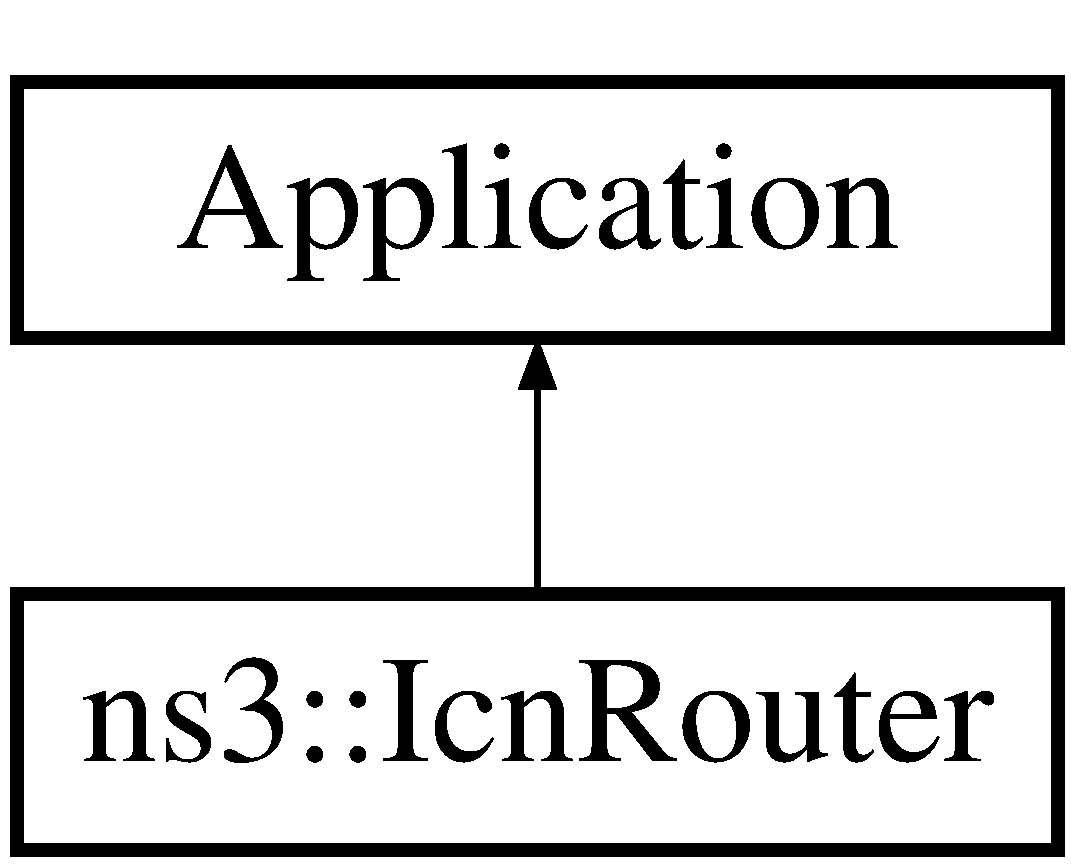
\includegraphics[height=2.000000cm]{classns3_1_1IcnRouter}
\end{center}
\end{figure}
\subsection*{Public Member Functions}
\begin{DoxyCompactItemize}
\item 
\hyperlink{classns3_1_1IcnRouter_a897987eb9c320461f49a23b1d7c98812}{Icn\-Router} ()
\item 
virtual \hyperlink{classns3_1_1IcnRouter_a52e01ead62ed2cf1d22ecba1e5c935f3}{$\sim$\-Icn\-Router} (void)
\item 
void \hyperlink{classns3_1_1IcnRouter_aee36cbcb810f960360aaf4a7efdcc237}{Read\-Packet} (Ptr$<$ Packet $>$ packet, Ipv4\-Address sender\-Address, uint16\-\_\-t sender\-Port)
\begin{DoxyCompactList}\small\item\em Read the recieved packet. If packet is content query packet from I\-C\-N Manager, it send the requested content to client address as mentioned in the packet. \end{DoxyCompactList}\item 
void \hyperlink{classns3_1_1IcnRouter_aaaf642b9d376e673288a2a5e28ac1b65}{Send\-Ack\-To\-Icn\-Manager} (Ipv4\-Address icn\-Manager\-Ipv4\-Address, uint16\-\_\-t icn\-Manager\-Port, \hyperlink{classns3_1_1DnsPlusQuestionHeader}{Dns\-Plus\-Question\-Header} dns\-Plus\-Question\-Header, \hyperlink{classns3_1_1DnsPlusHeader}{Dns\-Plus\-Header} dns\-Plus\-Header, \hyperlink{classns3_1_1OicnHeader}{Oicn\-Header} oicn\-Header)
\begin{DoxyCompactList}\small\item\em It send the A\-C\-K packet to I\-C\-N Manager stating that it has received the content query packet. \end{DoxyCompactList}\item 
void \hyperlink{classns3_1_1IcnRouter_ae0452d61162e9ce77690ecd06eff81d8}{Send\-To\-Client} (uint32\-\_\-t client\-Address, std\-::string name)
\begin{DoxyCompactList}\small\item\em It send the cached content to client as directed by the I\-C\-N Manager. \end{DoxyCompactList}\end{DoxyCompactItemize}
\subsection*{Static Public Member Functions}
\begin{DoxyCompactItemize}
\item 
static Type\-Id \hyperlink{classns3_1_1IcnRouter_af11ef09981ae023b6c9aaba3e1b02cb8}{Get\-Type\-Id} (void)
\begin{DoxyCompactList}\small\item\em Get the type I\-D. \end{DoxyCompactList}\end{DoxyCompactItemize}
\subsection*{Protected Member Functions}
\begin{DoxyCompactItemize}
\item 
virtual void \hyperlink{classns3_1_1IcnRouter_a753e828732d2efd5edf54965642a1605}{Do\-Dispose} (void)
\end{DoxyCompactItemize}
\subsection*{Private Member Functions}
\begin{DoxyCompactItemize}
\item 
void \hyperlink{classns3_1_1IcnRouter_ab7af309cff6c4061bb4ec42cacf2d149}{Handle\-Read\-Icn\-Manger} (Ptr$<$ Socket $>$ socket)
\begin{DoxyCompactList}\small\item\em Handle a packet reception. This function is called by lower layers. \end{DoxyCompactList}\item 
virtual void \hyperlink{classns3_1_1IcnRouter_a05d410c4dfb02bb8d7aaf6218ffb7254}{Start\-Application} (void)
\item 
virtual void \hyperlink{classns3_1_1IcnRouter_a92c56afe4750a18afca7ccca6410af46}{Stop\-Application} (void)
\end{DoxyCompactItemize}
\subsection*{Private Attributes}
\begin{DoxyCompactItemize}
\item 
Ptr$<$ Socket $>$ \hyperlink{classns3_1_1IcnRouter_a2b69d463e55b4be9f372c51bdb673d50}{m\-\_\-socket}
\begin{DoxyCompactList}\small\item\em socket \end{DoxyCompactList}\item 
Ptr$<$ Socket $>$ \hyperlink{classns3_1_1IcnRouter_ada56beecc0b64ce0ad38552c445dae88}{m\-\_\-socket\-Icn\-Manager}
\begin{DoxyCompactList}\small\item\em socket connected to I\-C\-N Manager \end{DoxyCompactList}\item 
uint16\-\_\-t \hyperlink{classns3_1_1IcnRouter_a793e6ef791d5581f4741e47cc969547e}{m\-\_\-port}
\begin{DoxyCompactList}\small\item\em I\-C\-N Router port it us defined as 89. \end{DoxyCompactList}\item 
uint16\-\_\-t \hyperlink{classns3_1_1IcnRouter_ab8a2228dfb2dda1af02f8017107d9f9a}{m\-\_\-client\-Port}
\begin{DoxyCompactList}\small\item\em I\-C\-N Client port defined as 26. \end{DoxyCompactList}\end{DoxyCompactItemize}


\subsection{Detailed Description}
I\-C\-N Router has the capability to cache the contents. 

\subsection{Constructor \& Destructor Documentation}
\hypertarget{classns3_1_1IcnRouter_a897987eb9c320461f49a23b1d7c98812}{\index{ns3\-::\-Icn\-Router@{ns3\-::\-Icn\-Router}!Icn\-Router@{Icn\-Router}}
\index{Icn\-Router@{Icn\-Router}!ns3::IcnRouter@{ns3\-::\-Icn\-Router}}
\subsubsection[{Icn\-Router}]{\setlength{\rightskip}{0pt plus 5cm}ns3\-::\-Icn\-Router\-::\-Icn\-Router (
\begin{DoxyParamCaption}
{}
\end{DoxyParamCaption}
)}}\label{classns3_1_1IcnRouter_a897987eb9c320461f49a23b1d7c98812}
\hypertarget{classns3_1_1IcnRouter_a52e01ead62ed2cf1d22ecba1e5c935f3}{\index{ns3\-::\-Icn\-Router@{ns3\-::\-Icn\-Router}!$\sim$\-Icn\-Router@{$\sim$\-Icn\-Router}}
\index{$\sim$\-Icn\-Router@{$\sim$\-Icn\-Router}!ns3::IcnRouter@{ns3\-::\-Icn\-Router}}
\subsubsection[{$\sim$\-Icn\-Router}]{\setlength{\rightskip}{0pt plus 5cm}ns3\-::\-Icn\-Router\-::$\sim$\-Icn\-Router (
\begin{DoxyParamCaption}
\item[{void}]{}
\end{DoxyParamCaption}
)\hspace{0.3cm}{\ttfamily [virtual]}}}\label{classns3_1_1IcnRouter_a52e01ead62ed2cf1d22ecba1e5c935f3}


\subsection{Member Function Documentation}
\hypertarget{classns3_1_1IcnRouter_a753e828732d2efd5edf54965642a1605}{\index{ns3\-::\-Icn\-Router@{ns3\-::\-Icn\-Router}!Do\-Dispose@{Do\-Dispose}}
\index{Do\-Dispose@{Do\-Dispose}!ns3::IcnRouter@{ns3\-::\-Icn\-Router}}
\subsubsection[{Do\-Dispose}]{\setlength{\rightskip}{0pt plus 5cm}void ns3\-::\-Icn\-Router\-::\-Do\-Dispose (
\begin{DoxyParamCaption}
\item[{void}]{}
\end{DoxyParamCaption}
)\hspace{0.3cm}{\ttfamily [protected]}, {\ttfamily [virtual]}}}\label{classns3_1_1IcnRouter_a753e828732d2efd5edf54965642a1605}
\hypertarget{classns3_1_1IcnRouter_af11ef09981ae023b6c9aaba3e1b02cb8}{\index{ns3\-::\-Icn\-Router@{ns3\-::\-Icn\-Router}!Get\-Type\-Id@{Get\-Type\-Id}}
\index{Get\-Type\-Id@{Get\-Type\-Id}!ns3::IcnRouter@{ns3\-::\-Icn\-Router}}
\subsubsection[{Get\-Type\-Id}]{\setlength{\rightskip}{0pt plus 5cm}Type\-Id ns3\-::\-Icn\-Router\-::\-Get\-Type\-Id (
\begin{DoxyParamCaption}
\item[{void}]{}
\end{DoxyParamCaption}
)\hspace{0.3cm}{\ttfamily [static]}}}\label{classns3_1_1IcnRouter_af11ef09981ae023b6c9aaba3e1b02cb8}


Get the type I\-D. 

\begin{DoxyReturn}{Returns}
the object Type\-Id 
\end{DoxyReturn}
\hypertarget{classns3_1_1IcnRouter_ab7af309cff6c4061bb4ec42cacf2d149}{\index{ns3\-::\-Icn\-Router@{ns3\-::\-Icn\-Router}!Handle\-Read\-Icn\-Manger@{Handle\-Read\-Icn\-Manger}}
\index{Handle\-Read\-Icn\-Manger@{Handle\-Read\-Icn\-Manger}!ns3::IcnRouter@{ns3\-::\-Icn\-Router}}
\subsubsection[{Handle\-Read\-Icn\-Manger}]{\setlength{\rightskip}{0pt plus 5cm}void ns3\-::\-Icn\-Router\-::\-Handle\-Read\-Icn\-Manger (
\begin{DoxyParamCaption}
\item[{Ptr$<$ Socket $>$}]{socket}
\end{DoxyParamCaption}
)\hspace{0.3cm}{\ttfamily [private]}}}\label{classns3_1_1IcnRouter_ab7af309cff6c4061bb4ec42cacf2d149}


Handle a packet reception. This function is called by lower layers. 


\begin{DoxyParams}{Parameters}
{\em socket} & the socket the packet was received to. \\
\hline
\end{DoxyParams}
\hypertarget{classns3_1_1IcnRouter_aee36cbcb810f960360aaf4a7efdcc237}{\index{ns3\-::\-Icn\-Router@{ns3\-::\-Icn\-Router}!Read\-Packet@{Read\-Packet}}
\index{Read\-Packet@{Read\-Packet}!ns3::IcnRouter@{ns3\-::\-Icn\-Router}}
\subsubsection[{Read\-Packet}]{\setlength{\rightskip}{0pt plus 5cm}void ns3\-::\-Icn\-Router\-::\-Read\-Packet (
\begin{DoxyParamCaption}
\item[{Ptr$<$ Packet $>$}]{packet, }
\item[{Ipv4\-Address}]{sender\-Address, }
\item[{uint16\-\_\-t}]{sender\-Port}
\end{DoxyParamCaption}
)}}\label{classns3_1_1IcnRouter_aee36cbcb810f960360aaf4a7efdcc237}


Read the recieved packet. If packet is content query packet from I\-C\-N Manager, it send the requested content to client address as mentioned in the packet. 


\begin{DoxyParams}{Parameters}
{\em packet} & packet received \\
\hline
{\em sender\-Address} & ipv4 address of sender \\
\hline
{\em port} & port of the sender \\
\hline
\end{DoxyParams}
\hypertarget{classns3_1_1IcnRouter_aaaf642b9d376e673288a2a5e28ac1b65}{\index{ns3\-::\-Icn\-Router@{ns3\-::\-Icn\-Router}!Send\-Ack\-To\-Icn\-Manager@{Send\-Ack\-To\-Icn\-Manager}}
\index{Send\-Ack\-To\-Icn\-Manager@{Send\-Ack\-To\-Icn\-Manager}!ns3::IcnRouter@{ns3\-::\-Icn\-Router}}
\subsubsection[{Send\-Ack\-To\-Icn\-Manager}]{\setlength{\rightskip}{0pt plus 5cm}void ns3\-::\-Icn\-Router\-::\-Send\-Ack\-To\-Icn\-Manager (
\begin{DoxyParamCaption}
\item[{Ipv4\-Address}]{icn\-Manager\-Ipv4\-Address, }
\item[{uint16\-\_\-t}]{icn\-Manager\-Port, }
\item[{{\bf Dns\-Plus\-Question\-Header}}]{dns\-Plus\-Question\-Header, }
\item[{{\bf Dns\-Plus\-Header}}]{dns\-Plus\-Header, }
\item[{{\bf Oicn\-Header}}]{oicn\-Header}
\end{DoxyParamCaption}
)}}\label{classns3_1_1IcnRouter_aaaf642b9d376e673288a2a5e28ac1b65}


It send the A\-C\-K packet to I\-C\-N Manager stating that it has received the content query packet. 


\begin{DoxyParams}{Parameters}
{\em icn\-Manager\-Ipv4\-Address} & I\-C\-N Manager Ipv4 address \\
\hline
{\em icn\-Manager\-Port} & I\-C\-N Manager port \\
\hline
{\em dns\-Plus\-Question\-Header} & Dns\-Plus Question header section \\
\hline
{\em dns\-Plus\-Header} & Dns\-Plus header section \\
\hline
{\em oicn\-Header} & O\-I\-C\-N header \\
\hline
\end{DoxyParams}
\hypertarget{classns3_1_1IcnRouter_ae0452d61162e9ce77690ecd06eff81d8}{\index{ns3\-::\-Icn\-Router@{ns3\-::\-Icn\-Router}!Send\-To\-Client@{Send\-To\-Client}}
\index{Send\-To\-Client@{Send\-To\-Client}!ns3::IcnRouter@{ns3\-::\-Icn\-Router}}
\subsubsection[{Send\-To\-Client}]{\setlength{\rightskip}{0pt plus 5cm}void ns3\-::\-Icn\-Router\-::\-Send\-To\-Client (
\begin{DoxyParamCaption}
\item[{uint32\-\_\-t}]{client\-Address, }
\item[{std\-::string}]{name}
\end{DoxyParamCaption}
)}}\label{classns3_1_1IcnRouter_ae0452d61162e9ce77690ecd06eff81d8}


It send the cached content to client as directed by the I\-C\-N Manager. 


\begin{DoxyParams}{Parameters}
{\em client\-Address} & client ipv4 address \\
\hline
{\em name} & name of the requested content \\
\hline
\end{DoxyParams}
\hypertarget{classns3_1_1IcnRouter_a05d410c4dfb02bb8d7aaf6218ffb7254}{\index{ns3\-::\-Icn\-Router@{ns3\-::\-Icn\-Router}!Start\-Application@{Start\-Application}}
\index{Start\-Application@{Start\-Application}!ns3::IcnRouter@{ns3\-::\-Icn\-Router}}
\subsubsection[{Start\-Application}]{\setlength{\rightskip}{0pt plus 5cm}void ns3\-::\-Icn\-Router\-::\-Start\-Application (
\begin{DoxyParamCaption}
\item[{void}]{}
\end{DoxyParamCaption}
)\hspace{0.3cm}{\ttfamily [private]}, {\ttfamily [virtual]}}}\label{classns3_1_1IcnRouter_a05d410c4dfb02bb8d7aaf6218ffb7254}
\hypertarget{classns3_1_1IcnRouter_a92c56afe4750a18afca7ccca6410af46}{\index{ns3\-::\-Icn\-Router@{ns3\-::\-Icn\-Router}!Stop\-Application@{Stop\-Application}}
\index{Stop\-Application@{Stop\-Application}!ns3::IcnRouter@{ns3\-::\-Icn\-Router}}
\subsubsection[{Stop\-Application}]{\setlength{\rightskip}{0pt plus 5cm}void ns3\-::\-Icn\-Router\-::\-Stop\-Application (
\begin{DoxyParamCaption}
\item[{void}]{}
\end{DoxyParamCaption}
)\hspace{0.3cm}{\ttfamily [private]}, {\ttfamily [virtual]}}}\label{classns3_1_1IcnRouter_a92c56afe4750a18afca7ccca6410af46}


\subsection{Member Data Documentation}
\hypertarget{classns3_1_1IcnRouter_ab8a2228dfb2dda1af02f8017107d9f9a}{\index{ns3\-::\-Icn\-Router@{ns3\-::\-Icn\-Router}!m\-\_\-client\-Port@{m\-\_\-client\-Port}}
\index{m\-\_\-client\-Port@{m\-\_\-client\-Port}!ns3::IcnRouter@{ns3\-::\-Icn\-Router}}
\subsubsection[{m\-\_\-client\-Port}]{\setlength{\rightskip}{0pt plus 5cm}uint16\-\_\-t ns3\-::\-Icn\-Router\-::m\-\_\-client\-Port\hspace{0.3cm}{\ttfamily [private]}}}\label{classns3_1_1IcnRouter_ab8a2228dfb2dda1af02f8017107d9f9a}


I\-C\-N Client port defined as 26. 

\hypertarget{classns3_1_1IcnRouter_a793e6ef791d5581f4741e47cc969547e}{\index{ns3\-::\-Icn\-Router@{ns3\-::\-Icn\-Router}!m\-\_\-port@{m\-\_\-port}}
\index{m\-\_\-port@{m\-\_\-port}!ns3::IcnRouter@{ns3\-::\-Icn\-Router}}
\subsubsection[{m\-\_\-port}]{\setlength{\rightskip}{0pt plus 5cm}uint16\-\_\-t ns3\-::\-Icn\-Router\-::m\-\_\-port\hspace{0.3cm}{\ttfamily [private]}}}\label{classns3_1_1IcnRouter_a793e6ef791d5581f4741e47cc969547e}


I\-C\-N Router port it us defined as 89. 

\hypertarget{classns3_1_1IcnRouter_a2b69d463e55b4be9f372c51bdb673d50}{\index{ns3\-::\-Icn\-Router@{ns3\-::\-Icn\-Router}!m\-\_\-socket@{m\-\_\-socket}}
\index{m\-\_\-socket@{m\-\_\-socket}!ns3::IcnRouter@{ns3\-::\-Icn\-Router}}
\subsubsection[{m\-\_\-socket}]{\setlength{\rightskip}{0pt plus 5cm}Ptr$<$Socket$>$ ns3\-::\-Icn\-Router\-::m\-\_\-socket\hspace{0.3cm}{\ttfamily [private]}}}\label{classns3_1_1IcnRouter_a2b69d463e55b4be9f372c51bdb673d50}


socket 

\hypertarget{classns3_1_1IcnRouter_ada56beecc0b64ce0ad38552c445dae88}{\index{ns3\-::\-Icn\-Router@{ns3\-::\-Icn\-Router}!m\-\_\-socket\-Icn\-Manager@{m\-\_\-socket\-Icn\-Manager}}
\index{m\-\_\-socket\-Icn\-Manager@{m\-\_\-socket\-Icn\-Manager}!ns3::IcnRouter@{ns3\-::\-Icn\-Router}}
\subsubsection[{m\-\_\-socket\-Icn\-Manager}]{\setlength{\rightskip}{0pt plus 5cm}Ptr$<$Socket$>$ ns3\-::\-Icn\-Router\-::m\-\_\-socket\-Icn\-Manager\hspace{0.3cm}{\ttfamily [private]}}}\label{classns3_1_1IcnRouter_ada56beecc0b64ce0ad38552c445dae88}


socket connected to I\-C\-N Manager 



The documentation for this class was generated from the following files\-:\begin{DoxyCompactItemize}
\item 
model/\hyperlink{icn-router_8h}{icn-\/router.\-h}\item 
model/\hyperlink{icn-router_8cc}{icn-\/router.\-cc}\end{DoxyCompactItemize}

\hypertarget{classns3_1_1IcnRouterHelpher}{\section{ns3\-:\-:Icn\-Router\-Helpher Class Reference}
\label{classns3_1_1IcnRouterHelpher}\index{ns3\-::\-Icn\-Router\-Helpher@{ns3\-::\-Icn\-Router\-Helpher}}
}


I\-C\-N Router has the capability to cache the contents.  




{\ttfamily \#include $<$oicn-\/application-\/helper.\-h$>$}

\subsection*{Public Member Functions}
\begin{DoxyCompactItemize}
\item 
\hyperlink{classns3_1_1IcnRouterHelpher_a3cb1509ce406113dd7d7b9cfe07b76b1}{Icn\-Router\-Helpher} ()
\item 
void \hyperlink{classns3_1_1IcnRouterHelpher_aa2820444ac554e404d9fd6ce5f8a8fe6}{Set\-Attribute} (std\-::string name, const Attribute\-Value \&value)
\item 
Application\-Container \hyperlink{classns3_1_1IcnRouterHelpher_acef840c519effa743944c8e6eb1a422b}{Install} (Ptr$<$ Node $>$ node) const 
\item 
Application\-Container \hyperlink{classns3_1_1IcnRouterHelpher_acbe0017e55f293cd2c61aee1263e1878}{Install} (std\-::string node\-Name) const 
\item 
Application\-Container \hyperlink{classns3_1_1IcnRouterHelpher_a0846f519c253e08ceb8292aee2e46b67}{Install} (Node\-Container c) const 
\end{DoxyCompactItemize}
\subsection*{Private Member Functions}
\begin{DoxyCompactItemize}
\item 
Application\-Container \hyperlink{classns3_1_1IcnRouterHelpher_ade395ffa9be3d533ff54253fb2eb2b33}{Install\-Priv} (Ptr$<$ Node $>$ node) const 
\end{DoxyCompactItemize}
\subsection*{Private Attributes}
\begin{DoxyCompactItemize}
\item 
Object\-Factory \hyperlink{classns3_1_1IcnRouterHelpher_a1a9a541fc339cb6541195330b1c74009}{m\-\_\-factory}
\begin{DoxyCompactList}\small\item\em Object factory. \end{DoxyCompactList}\end{DoxyCompactItemize}


\subsection{Detailed Description}
I\-C\-N Router has the capability to cache the contents. 

\subsection{Constructor \& Destructor Documentation}
\hypertarget{classns3_1_1IcnRouterHelpher_a3cb1509ce406113dd7d7b9cfe07b76b1}{\index{ns3\-::\-Icn\-Router\-Helpher@{ns3\-::\-Icn\-Router\-Helpher}!Icn\-Router\-Helpher@{Icn\-Router\-Helpher}}
\index{Icn\-Router\-Helpher@{Icn\-Router\-Helpher}!ns3::IcnRouterHelpher@{ns3\-::\-Icn\-Router\-Helpher}}
\subsubsection[{Icn\-Router\-Helpher}]{\setlength{\rightskip}{0pt plus 5cm}ns3\-::\-Icn\-Router\-Helpher\-::\-Icn\-Router\-Helpher (
\begin{DoxyParamCaption}
{}
\end{DoxyParamCaption}
)}}\label{classns3_1_1IcnRouterHelpher_a3cb1509ce406113dd7d7b9cfe07b76b1}


\subsection{Member Function Documentation}
\hypertarget{classns3_1_1IcnRouterHelpher_acef840c519effa743944c8e6eb1a422b}{\index{ns3\-::\-Icn\-Router\-Helpher@{ns3\-::\-Icn\-Router\-Helpher}!Install@{Install}}
\index{Install@{Install}!ns3::IcnRouterHelpher@{ns3\-::\-Icn\-Router\-Helpher}}
\subsubsection[{Install}]{\setlength{\rightskip}{0pt plus 5cm}Application\-Container ns3\-::\-Icn\-Router\-Helpher\-::\-Install (
\begin{DoxyParamCaption}
\item[{Ptr$<$ Node $>$}]{node}
\end{DoxyParamCaption}
) const}}\label{classns3_1_1IcnRouterHelpher_acef840c519effa743944c8e6eb1a422b}
Create an I\-C\-N Router Application


\begin{DoxyParams}{Parameters}
{\em node} & the node on which to create the Application. The node is specified by a Ptr$<$\-Node$>$. \\
\hline
\end{DoxyParams}
\begin{DoxyReturn}{Returns}
an Application\-Container holding the Application created 
\end{DoxyReturn}
\hypertarget{classns3_1_1IcnRouterHelpher_acbe0017e55f293cd2c61aee1263e1878}{\index{ns3\-::\-Icn\-Router\-Helpher@{ns3\-::\-Icn\-Router\-Helpher}!Install@{Install}}
\index{Install@{Install}!ns3::IcnRouterHelpher@{ns3\-::\-Icn\-Router\-Helpher}}
\subsubsection[{Install}]{\setlength{\rightskip}{0pt plus 5cm}Application\-Container ns3\-::\-Icn\-Router\-Helpher\-::\-Install (
\begin{DoxyParamCaption}
\item[{std\-::string}]{node\-Name}
\end{DoxyParamCaption}
) const}}\label{classns3_1_1IcnRouterHelpher_acbe0017e55f293cd2c61aee1263e1878}
Create an I\-C\-N Router Application 
\begin{DoxyParams}{Parameters}
{\em node\-Name} & the name of the node on which to create the application \\
\hline
\end{DoxyParams}
\begin{DoxyReturn}{Returns}
an Application\-Container holding the Application created 
\end{DoxyReturn}
\hypertarget{classns3_1_1IcnRouterHelpher_a0846f519c253e08ceb8292aee2e46b67}{\index{ns3\-::\-Icn\-Router\-Helpher@{ns3\-::\-Icn\-Router\-Helpher}!Install@{Install}}
\index{Install@{Install}!ns3::IcnRouterHelpher@{ns3\-::\-Icn\-Router\-Helpher}}
\subsubsection[{Install}]{\setlength{\rightskip}{0pt plus 5cm}Application\-Container ns3\-::\-Icn\-Router\-Helpher\-::\-Install (
\begin{DoxyParamCaption}
\item[{Node\-Container}]{c}
\end{DoxyParamCaption}
) const}}\label{classns3_1_1IcnRouterHelpher_a0846f519c253e08ceb8292aee2e46b67}
Create an I\-C\-N Router Application 
\begin{DoxyParams}{Parameters}
{\em c} & the nodes on which to create the Applications. The nodes are specified by a Node\-Container. \\
\hline
\end{DoxyParams}
\begin{DoxyReturn}{Returns}
an Application\-Container holding the Application created 
\end{DoxyReturn}
\hypertarget{classns3_1_1IcnRouterHelpher_ade395ffa9be3d533ff54253fb2eb2b33}{\index{ns3\-::\-Icn\-Router\-Helpher@{ns3\-::\-Icn\-Router\-Helpher}!Install\-Priv@{Install\-Priv}}
\index{Install\-Priv@{Install\-Priv}!ns3::IcnRouterHelpher@{ns3\-::\-Icn\-Router\-Helpher}}
\subsubsection[{Install\-Priv}]{\setlength{\rightskip}{0pt plus 5cm}Application\-Container ns3\-::\-Icn\-Router\-Helpher\-::\-Install\-Priv (
\begin{DoxyParamCaption}
\item[{Ptr$<$ Node $>$}]{node}
\end{DoxyParamCaption}
) const\hspace{0.3cm}{\ttfamily [private]}}}\label{classns3_1_1IcnRouterHelpher_ade395ffa9be3d533ff54253fb2eb2b33}
Install an I\-C\-N Router Application on the node configured with all the attributes set with Set\-Attribute. 
\begin{DoxyParams}{Parameters}
{\em node} & the node on which an O\-I\-C\-N\-Client will be installed. \\
\hline
\end{DoxyParams}
\begin{DoxyReturn}{Returns}
an Application\-Container holding the Application created 
\end{DoxyReturn}
\hypertarget{classns3_1_1IcnRouterHelpher_aa2820444ac554e404d9fd6ce5f8a8fe6}{\index{ns3\-::\-Icn\-Router\-Helpher@{ns3\-::\-Icn\-Router\-Helpher}!Set\-Attribute@{Set\-Attribute}}
\index{Set\-Attribute@{Set\-Attribute}!ns3::IcnRouterHelpher@{ns3\-::\-Icn\-Router\-Helpher}}
\subsubsection[{Set\-Attribute}]{\setlength{\rightskip}{0pt plus 5cm}void ns3\-::\-Icn\-Router\-Helpher\-::\-Set\-Attribute (
\begin{DoxyParamCaption}
\item[{std\-::string}]{name, }
\item[{const Attribute\-Value \&}]{value}
\end{DoxyParamCaption}
)}}\label{classns3_1_1IcnRouterHelpher_aa2820444ac554e404d9fd6ce5f8a8fe6}
Record an attribute to be set in each Application after it is is created.


\begin{DoxyParams}{Parameters}
{\em name} & the name of the attribute to set \\
\hline
{\em value} & the value of the attribute to set \\
\hline
\end{DoxyParams}


\subsection{Member Data Documentation}
\hypertarget{classns3_1_1IcnRouterHelpher_a1a9a541fc339cb6541195330b1c74009}{\index{ns3\-::\-Icn\-Router\-Helpher@{ns3\-::\-Icn\-Router\-Helpher}!m\-\_\-factory@{m\-\_\-factory}}
\index{m\-\_\-factory@{m\-\_\-factory}!ns3::IcnRouterHelpher@{ns3\-::\-Icn\-Router\-Helpher}}
\subsubsection[{m\-\_\-factory}]{\setlength{\rightskip}{0pt plus 5cm}Object\-Factory ns3\-::\-Icn\-Router\-Helpher\-::m\-\_\-factory\hspace{0.3cm}{\ttfamily [private]}}}\label{classns3_1_1IcnRouterHelpher_a1a9a541fc339cb6541195330b1c74009}


Object factory. 



The documentation for this class was generated from the following files\-:\begin{DoxyCompactItemize}
\item 
helper/\hyperlink{oicn-application-helper_8h}{oicn-\/application-\/helper.\-h}\item 
helper/\hyperlink{oicn-application-helper_8cc}{oicn-\/application-\/helper.\-cc}\end{DoxyCompactItemize}

\hypertarget{classns3_1_1Ipv4RouterL3Protocol}{\section{ns3\-:\-:Ipv4\-Router\-L3\-Protocol Class Reference}
\label{classns3_1_1Ipv4RouterL3Protocol}\index{ns3\-::\-Ipv4\-Router\-L3\-Protocol@{ns3\-::\-Ipv4\-Router\-L3\-Protocol}}
}


Implement the Ipv4 layer in an I\-C\-N Router.  




{\ttfamily \#include $<$ipv4-\/router-\/l3-\/protocol.\-h$>$}

Inheritance diagram for ns3\-:\-:Ipv4\-Router\-L3\-Protocol\-:\begin{figure}[H]
\begin{center}
\leavevmode
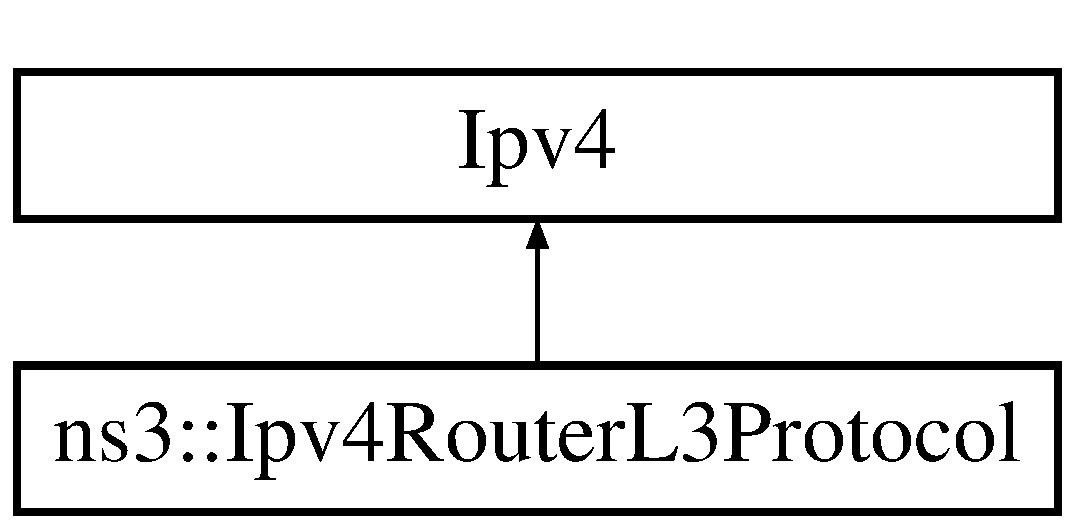
\includegraphics[height=2.000000cm]{classns3_1_1Ipv4RouterL3Protocol}
\end{center}
\end{figure}
\subsection*{Classes}
\begin{DoxyCompactItemize}
\item 
class \hyperlink{classns3_1_1Ipv4RouterL3Protocol_1_1Fragments}{Fragments}
\begin{DoxyCompactList}\small\item\em A Set of Fragment belonging to the same packet (src, dst, identification and proto) \end{DoxyCompactList}\end{DoxyCompactItemize}
\subsection*{Public Types}
\begin{DoxyCompactItemize}
\item 
enum \hyperlink{classns3_1_1Ipv4RouterL3Protocol_a050d08aa42fe2c3f9c133a263e121fcd}{Drop\-Reason} \{ \\*
\hyperlink{classns3_1_1Ipv4RouterL3Protocol_a050d08aa42fe2c3f9c133a263e121fcdaa4940eaf513382cd5e6d580a12610c21}{D\-R\-O\-P\-\_\-\-T\-T\-L\-\_\-\-E\-X\-P\-I\-R\-E\-D} = 1, 
\hyperlink{classns3_1_1Ipv4RouterL3Protocol_a050d08aa42fe2c3f9c133a263e121fcdaed5a0bb11a898cfc1050d9087a5030dc}{D\-R\-O\-P\-\_\-\-N\-O\-\_\-\-R\-O\-U\-T\-E}, 
\hyperlink{classns3_1_1Ipv4RouterL3Protocol_a050d08aa42fe2c3f9c133a263e121fcdaa7a09de0c3a08a72d5e443151d0d9f95}{D\-R\-O\-P\-\_\-\-B\-A\-D\-\_\-\-C\-H\-E\-C\-K\-S\-U\-M}, 
\hyperlink{classns3_1_1Ipv4RouterL3Protocol_a050d08aa42fe2c3f9c133a263e121fcdab55f6d41f00ca4c6ab4a2211ec9ee1f2}{D\-R\-O\-P\-\_\-\-I\-N\-T\-E\-R\-F\-A\-C\-E\-\_\-\-D\-O\-W\-N}, 
\\*
\hyperlink{classns3_1_1Ipv4RouterL3Protocol_a050d08aa42fe2c3f9c133a263e121fcda9543ec21a03e3ee4a394152ca8f15a95}{D\-R\-O\-P\-\_\-\-R\-O\-U\-T\-E\-\_\-\-E\-R\-R\-O\-R}, 
\hyperlink{classns3_1_1Ipv4RouterL3Protocol_a050d08aa42fe2c3f9c133a263e121fcda5616817187e3e89a1e76e65d30293abe}{D\-R\-O\-P\-\_\-\-F\-R\-A\-G\-M\-E\-N\-T\-\_\-\-T\-I\-M\-E\-O\-U\-T}
 \}
\begin{DoxyCompactList}\small\item\em Reason why a packet has been dropped. \end{DoxyCompactList}\end{DoxyCompactItemize}
\subsection*{Public Member Functions}
\begin{DoxyCompactItemize}
\item 
\hyperlink{classns3_1_1Ipv4RouterL3Protocol_a91b2d31fa02934b841bbe50f218c4981}{Ipv4\-Router\-L3\-Protocol} ()
\item 
virtual \hyperlink{classns3_1_1Ipv4RouterL3Protocol_ab3ce503154a7dc7ed8f0f78dc42f6554}{$\sim$\-Ipv4\-Router\-L3\-Protocol} ()
\item 
void \hyperlink{classns3_1_1Ipv4RouterL3Protocol_ac5411f9b064b86f0975582571cd0b6de}{Set\-Node} (Ptr$<$ Node $>$ node)
\begin{DoxyCompactList}\small\item\em Set node associated with this stack. \end{DoxyCompactList}\item 
void \hyperlink{classns3_1_1Ipv4RouterL3Protocol_adf92410e6c028eaf5f70e3c704009680}{Set\-Routing\-Protocol} (Ptr$<$ Ipv4\-Routing\-Protocol $>$ routing\-Protocol)
\item 
Ptr$<$ Ipv4\-Routing\-Protocol $>$ \hyperlink{classns3_1_1Ipv4RouterL3Protocol_a2ed4d1c2d32115e0346bebef4b9de285}{Get\-Routing\-Protocol} (void) const 
\item 
Ptr$<$ Socket $>$ \hyperlink{classns3_1_1Ipv4RouterL3Protocol_aaa5ba602f884d731b2a8b69a3827b8a6}{Create\-Raw\-Socket} (void)
\item 
void \hyperlink{classns3_1_1Ipv4RouterL3Protocol_ac15242f30514a7656194efd4736d54e5}{Delete\-Raw\-Socket} (Ptr$<$ Socket $>$ socket)
\item 
void \hyperlink{classns3_1_1Ipv4RouterL3Protocol_aadadfecb7f1ad23a55f2faabb67efc37}{Insert} (Ptr$<$ Ip\-L4\-Protocol $>$ protocol)
\item 
virtual Ptr$<$ Ip\-L4\-Protocol $>$ \hyperlink{classns3_1_1Ipv4RouterL3Protocol_a117b7e10f49fa524ac465d3d9a41d990}{Get\-Protocol} (int protocol\-Number) const 
\item 
void \hyperlink{classns3_1_1Ipv4RouterL3Protocol_a8102bc7eb7d7267472b73bb10ef13d06}{Remove} (Ptr$<$ Ip\-L4\-Protocol $>$ protocol)
\item 
void \hyperlink{classns3_1_1Ipv4RouterL3Protocol_a6c1add6164864dceeb83d5fa8bbdd59a}{Set\-Default\-Ttl} (uint8\-\_\-t ttl)
\item 
void \hyperlink{classns3_1_1Ipv4RouterL3Protocol_a30dd164d51b321d117bd06cfedd6e1f5}{Receive} (Ptr$<$ Net\-Device $>$ device, Ptr$<$ const Packet $>$ p, uint16\-\_\-t protocol, const Address \&from, const Address \&to, Net\-Device\-::\-Packet\-Type packet\-Type)
\item 
void \hyperlink{classns3_1_1Ipv4RouterL3Protocol_a70f114cbb01fb2e2fbb21448355f75ff}{Send} (Ptr$<$ Packet $>$ packet, Ipv4\-Address source, Ipv4\-Address destination, uint8\-\_\-t protocol, Ptr$<$ Ipv4\-Route $>$ route)
\item 
void \hyperlink{classns3_1_1Ipv4RouterL3Protocol_a14b4a2978628ddebefbf5c32e3519c6a}{Send\-With\-Header} (Ptr$<$ Packet $>$ packet, Ipv4\-Header ip\-Header, Ptr$<$ Ipv4\-Route $>$ route)
\item 
uint32\-\_\-t \hyperlink{classns3_1_1Ipv4RouterL3Protocol_acb5095a80758a3ea89e8c8098e547ba4}{Add\-Interface} (Ptr$<$ Net\-Device $>$ device)
\item 
Ptr$<$ Ipv4\-Interface $>$ \hyperlink{classns3_1_1Ipv4RouterL3Protocol_a055c2bacc5bfda60b1a3b62d5233a048}{Get\-Interface} (uint32\-\_\-t i) const 
\begin{DoxyCompactList}\small\item\em Get an interface. \end{DoxyCompactList}\item 
uint32\-\_\-t \hyperlink{classns3_1_1Ipv4RouterL3Protocol_a1af4b8ab112a41d2c9c5caf45af6ba09}{Get\-N\-Interfaces} (void) const 
\item 
int32\-\_\-t \hyperlink{classns3_1_1Ipv4RouterL3Protocol_a811c4a2df331f426ac54eefd888f4b7a}{Get\-Interface\-For\-Address} (Ipv4\-Address addr) const 
\item 
int32\-\_\-t \hyperlink{classns3_1_1Ipv4RouterL3Protocol_a2c0e4620075ca23dc5290af5f18803b8}{Get\-Interface\-For\-Prefix} (Ipv4\-Address addr, Ipv4\-Mask mask) const 
\item 
int32\-\_\-t \hyperlink{classns3_1_1Ipv4RouterL3Protocol_abb943336599855e99db9a170783001c0}{Get\-Interface\-For\-Device} (Ptr$<$ const Net\-Device $>$ device) const 
\item 
bool \hyperlink{classns3_1_1Ipv4RouterL3Protocol_a5d1404a95b8f2ec49aaf4b4b603f9e21}{Is\-Destination\-Address} (Ipv4\-Address address, uint32\-\_\-t iif) const 
\item 
bool \hyperlink{classns3_1_1Ipv4RouterL3Protocol_ae78b4bd47fe0e723207a78d9ea4709b4}{Add\-Address} (uint32\-\_\-t i, Ipv4\-Interface\-Address address)
\item 
Ipv4\-Interface\-Address \hyperlink{classns3_1_1Ipv4RouterL3Protocol_a2eae427d44acd2cfb2954089ce89211d}{Get\-Address} (uint32\-\_\-t interface\-Index, uint32\-\_\-t address\-Index) const 
\item 
uint32\-\_\-t \hyperlink{classns3_1_1Ipv4RouterL3Protocol_a34f9fa2ed643bf8f7c13bddf1461a1b9}{Get\-N\-Addresses} (uint32\-\_\-t interface) const 
\item 
bool \hyperlink{classns3_1_1Ipv4RouterL3Protocol_a78a2d198be0f25c16037f98323b45ea2}{Remove\-Address} (uint32\-\_\-t interface\-Index, uint32\-\_\-t address\-Index)
\item 
bool \hyperlink{classns3_1_1Ipv4RouterL3Protocol_a81bad2ef6599a38a7b35fe8b0ce8d30f}{Remove\-Address} (uint32\-\_\-t interface, Ipv4\-Address address)
\item 
Ipv4\-Address \hyperlink{classns3_1_1Ipv4RouterL3Protocol_ad7287d5d0a844bb61fd72476ad8e9ee7}{Select\-Source\-Address} (Ptr$<$ const Net\-Device $>$ device, Ipv4\-Address dst, Ipv4\-Interface\-Address\-::\-Interface\-Address\-Scope\-\_\-e scope)
\item 
void \hyperlink{classns3_1_1Ipv4RouterL3Protocol_a5bbc44739ecc7fe8e995e5f5dcd9ce89}{Set\-Metric} (uint32\-\_\-t i, uint16\-\_\-t metric)
\item 
uint16\-\_\-t \hyperlink{classns3_1_1Ipv4RouterL3Protocol_a046d9e4b77a15e4d3bee2e415c8070c3}{Get\-Metric} (uint32\-\_\-t i) const 
\item 
uint16\-\_\-t \hyperlink{classns3_1_1Ipv4RouterL3Protocol_a9624b73c4e19e1a4c4155c2b6f35c76d}{Get\-Mtu} (uint32\-\_\-t i) const 
\item 
bool \hyperlink{classns3_1_1Ipv4RouterL3Protocol_a046298cf4c213797e047e7344701c8f5}{Is\-Up} (uint32\-\_\-t i) const 
\item 
void \hyperlink{classns3_1_1Ipv4RouterL3Protocol_a3352a473d2724c3e90f13e7116be3b5c}{Set\-Up} (uint32\-\_\-t i)
\item 
void \hyperlink{classns3_1_1Ipv4RouterL3Protocol_a88b0686519678bbe3e3a10aa82bf5cea}{Set\-Down} (uint32\-\_\-t i)
\item 
bool \hyperlink{classns3_1_1Ipv4RouterL3Protocol_a3a0efdbc3ff924c388a0db9bd8387aea}{Is\-Forwarding} (uint32\-\_\-t i) const 
\item 
void \hyperlink{classns3_1_1Ipv4RouterL3Protocol_aba2f18e349db994598b8b715e0557ac9}{Set\-Forwarding} (uint32\-\_\-t i, bool val)
\item 
Ptr$<$ Net\-Device $>$ \hyperlink{classns3_1_1Ipv4RouterL3Protocol_a6e4db6eb5d22d3ef5f9fba31c347ba00}{Get\-Net\-Device} (uint32\-\_\-t i)
\item 
bool \hyperlink{classns3_1_1Ipv4RouterL3Protocol_af45da819ef800c1fa6652ff38acd0abe}{Is\-Unicast} (Ipv4\-Address ad) const 
\begin{DoxyCompactList}\small\item\em Check if an I\-Pv4 address is unicast according to the node. \end{DoxyCompactList}\end{DoxyCompactItemize}
\subsection*{Static Public Member Functions}
\begin{DoxyCompactItemize}
\item 
static Type\-Id \hyperlink{classns3_1_1Ipv4RouterL3Protocol_a71648ed3ff5bcca634fe8ad5bfaed3f4}{Get\-Type\-Id} (void)
\begin{DoxyCompactList}\small\item\em Get the type I\-D. \end{DoxyCompactList}\end{DoxyCompactItemize}
\subsection*{Static Public Attributes}
\begin{DoxyCompactItemize}
\item 
static const uint16\-\_\-t \hyperlink{classns3_1_1Ipv4RouterL3Protocol_a2fdda6f3cb6e421706acf29bf38e8cd4}{P\-R\-O\-T\-\_\-\-N\-U\-M\-B\-E\-R} = 0x0800
\begin{DoxyCompactList}\small\item\em Protocol number (0x0800) \end{DoxyCompactList}\end{DoxyCompactItemize}
\subsection*{Protected Member Functions}
\begin{DoxyCompactItemize}
\item 
virtual void \hyperlink{classns3_1_1Ipv4RouterL3Protocol_ab4177a69c5d6de8f7453a59edcfafe41}{Do\-Dispose} (void)
\item 
virtual void \hyperlink{classns3_1_1Ipv4RouterL3Protocol_a37e6bad738c75f2ab56badba0e544d73}{Notify\-New\-Aggregate} ()
\end{DoxyCompactItemize}
\subsection*{Private Types}
\begin{DoxyCompactItemize}
\item 
typedef std\-::vector$<$ Ptr\\*
$<$ Ipv4\-Interface $>$ $>$ \hyperlink{classns3_1_1Ipv4RouterL3Protocol_a5756b4cefb3bc08242fcc25ce0694adb}{Ipv4\-Interface\-List}
\begin{DoxyCompactList}\small\item\em Container of the I\-Pv4 Interfaces. \end{DoxyCompactList}\item 
typedef std\-::list$<$ Ptr\\*
$<$ Ipv4\-Raw\-Socket\-Impl $>$ $>$ \hyperlink{classns3_1_1Ipv4RouterL3Protocol_aeaeda330ab6a6f6d7cf4392024f4dc8e}{Socket\-List}
\begin{DoxyCompactList}\small\item\em Container of the I\-Pv4 Raw Sockets. \end{DoxyCompactList}\item 
typedef std\-::list$<$ Ptr\\*
$<$ Ip\-L4\-Protocol $>$ $>$ \hyperlink{classns3_1_1Ipv4RouterL3Protocol_adec096bbe99d3a07e5007ce510a9ca20}{L4\-List\-\_\-t}
\begin{DoxyCompactList}\small\item\em Container of the I\-Pv4 L4 instances. \end{DoxyCompactList}\item 
typedef std\-::map$<$ std\-::pair\\*
$<$ uint64\-\_\-t, uint32\-\_\-t $>$, Ptr\\*
$<$ \hyperlink{classns3_1_1Ipv4RouterL3Protocol_1_1Fragments}{Fragments} $>$ $>$ \hyperlink{classns3_1_1Ipv4RouterL3Protocol_ad13f1d7a6fde1bccea2a986f095bbf9e}{Map\-Fragments\-\_\-t}
\begin{DoxyCompactList}\small\item\em Container of fragments, stored as pairs(src+dst addr, src+dst port) / fragment. \end{DoxyCompactList}\item 
typedef std\-::map$<$ std\-::pair\\*
$<$ uint64\-\_\-t, uint32\-\_\-t $>$\\*
, Event\-Id $>$ \hyperlink{classns3_1_1Ipv4RouterL3Protocol_a1b7e366a2a7bbb1336aacaca4af8997b}{Map\-Fragments\-Timers\-\_\-t}
\begin{DoxyCompactList}\small\item\em Container of fragment timeout event, stored as pairs(src+dst addr, src+dst port) / Event\-Id. \end{DoxyCompactList}\end{DoxyCompactItemize}
\subsection*{Private Member Functions}
\begin{DoxyCompactItemize}
\item 
\hyperlink{classns3_1_1Ipv4RouterL3Protocol_a018ab17a0a3160669b90ee6171c86aca}{Ipv4\-Router\-L3\-Protocol} (const \hyperlink{classns3_1_1Ipv4RouterL3Protocol}{Ipv4\-Router\-L3\-Protocol} \&)
\begin{DoxyCompactList}\small\item\em Copy constructor. \end{DoxyCompactList}\item 
\hyperlink{classns3_1_1Ipv4RouterL3Protocol}{Ipv4\-Router\-L3\-Protocol} \& \hyperlink{classns3_1_1Ipv4RouterL3Protocol_aa40baa411eeb3351bc5a2b5e0e1e9a5f}{operator=} (const \hyperlink{classns3_1_1Ipv4RouterL3Protocol}{Ipv4\-Router\-L3\-Protocol} \&)
\begin{DoxyCompactList}\small\item\em Copy constructor. \end{DoxyCompactList}\item 
virtual void \hyperlink{classns3_1_1Ipv4RouterL3Protocol_afea7958043ce0d38eb31f4440ea77abf}{Set\-Ip\-Forward} (bool forward)
\item 
virtual bool \hyperlink{classns3_1_1Ipv4RouterL3Protocol_a9402a1e20d4654777690f3325160045f}{Get\-Ip\-Forward} (void) const 
\item 
virtual void \hyperlink{classns3_1_1Ipv4RouterL3Protocol_a5d0537c163f0a6f04c2f0c5601075d2d}{Set\-Weak\-Es\-Model} (bool model)
\item 
virtual bool \hyperlink{classns3_1_1Ipv4RouterL3Protocol_a8023a88747b29737972a1d803daf9dcb}{Get\-Weak\-Es\-Model} (void) const 
\item 
Ipv4\-Header \hyperlink{classns3_1_1Ipv4RouterL3Protocol_a45fa0dd63568af0c2d0c4a7142072631}{Build\-Header} (Ipv4\-Address source, Ipv4\-Address destination, uint8\-\_\-t protocol, uint16\-\_\-t payload\-Size, uint8\-\_\-t ttl, uint8\-\_\-t tos, bool may\-Fragment)
\begin{DoxyCompactList}\small\item\em Construct an I\-Pv4 header. \end{DoxyCompactList}\item 
void \hyperlink{classns3_1_1Ipv4RouterL3Protocol_a35646708634f0d7008322bb34a4dc799}{Send\-Real\-Out} (Ptr$<$ Ipv4\-Route $>$ route, Ptr$<$ Packet $>$ packet, Ipv4\-Header const \&ip\-Header)
\begin{DoxyCompactList}\small\item\em Send packet with route. \end{DoxyCompactList}\item 
void \hyperlink{classns3_1_1Ipv4RouterL3Protocol_a85559a2c92f1c2ff3d80a1228ca6b634}{Ip\-Forward} (Ptr$<$ Ipv4\-Route $>$ rtentry, Ptr$<$ const Packet $>$ p, const Ipv4\-Header \&header)
\begin{DoxyCompactList}\small\item\em Forward a packet. \end{DoxyCompactList}\item 
void \hyperlink{classns3_1_1Ipv4RouterL3Protocol_a7cfc75feda36ad3c0c11cd5bf92e63f2}{Ip\-Multicast\-Forward} (Ptr$<$ Ipv4\-Multicast\-Route $>$ mrtentry, Ptr$<$ const Packet $>$ p, const Ipv4\-Header \&header)
\begin{DoxyCompactList}\small\item\em Forward a multicast packet. \end{DoxyCompactList}\item 
void \hyperlink{classns3_1_1Ipv4RouterL3Protocol_a89499fe56b8b356bb2190d311cf2a43c}{Local\-Deliver} (Ptr$<$ const Packet $>$ p, Ipv4\-Header const \&ip, uint32\-\_\-t iif)
\begin{DoxyCompactList}\small\item\em Deliver a packet. \end{DoxyCompactList}\item 
void \hyperlink{classns3_1_1Ipv4RouterL3Protocol_a96be298c33d8b9ebc2696d24b953cf4b}{Route\-Input\-Error} (Ptr$<$ const Packet $>$ p, const Ipv4\-Header \&ip\-Header, Socket\-::\-Socket\-Errno sock\-Errno)
\begin{DoxyCompactList}\small\item\em Fallback when no route is found. \end{DoxyCompactList}\item 
uint32\-\_\-t \hyperlink{classns3_1_1Ipv4RouterL3Protocol_a52bc289137d131894c462f1ea4089a36}{Add\-Ipv4\-Interface} (Ptr$<$ Ipv4\-Interface $>$ interface)
\begin{DoxyCompactList}\small\item\em Add an I\-Pv4 interface to the stack. \end{DoxyCompactList}\item 
void \hyperlink{classns3_1_1Ipv4RouterL3Protocol_ae038fa89483a01c2a8d1adc3d54dede6}{Setup\-Loopback} (void)
\begin{DoxyCompactList}\small\item\em Setup loopback interface. \end{DoxyCompactList}\item 
Ptr$<$ Icmpv4\-L4\-Protocol $>$ \hyperlink{classns3_1_1Ipv4RouterL3Protocol_aa8e6f15b2933344444970aed21d8641b}{Get\-Icmp} (void) const 
\begin{DoxyCompactList}\small\item\em Get I\-C\-M\-Pv4 protocol. \end{DoxyCompactList}\item 
bool \hyperlink{classns3_1_1Ipv4RouterL3Protocol_a94898bc72665a0aa0f03d8ff15abd398}{Is\-Unicast} (Ipv4\-Address ad, Ipv4\-Mask interface\-Mask) const 
\begin{DoxyCompactList}\small\item\em Check if an I\-Pv4 address is unicast. \end{DoxyCompactList}\item 
void \hyperlink{classns3_1_1Ipv4RouterL3Protocol_aeefc9ca2a1cbc6fbd8a676f1bab18313}{Do\-Fragmentation} (Ptr$<$ Packet $>$ packet, uint32\-\_\-t out\-Iface\-Mtu, std\-::list$<$ Ptr$<$ Packet $>$ $>$ \&list\-Fragments)
\begin{DoxyCompactList}\small\item\em Fragment a packet. \end{DoxyCompactList}\item 
bool \hyperlink{classns3_1_1Ipv4RouterL3Protocol_a859787bf309c07234ea58e62d26634a0}{Process\-Fragment} (Ptr$<$ Packet $>$ \&packet, Ipv4\-Header \&ip\-Header, uint32\-\_\-t iif)
\begin{DoxyCompactList}\small\item\em Process a packet fragment. \end{DoxyCompactList}\item 
void \hyperlink{classns3_1_1Ipv4RouterL3Protocol_ac4719458e3fdcd9d7d696a070c479747}{Handle\-Fragments\-Timeout} (std\-::pair$<$ uint64\-\_\-t, uint32\-\_\-t $>$ key, Ipv4\-Header \&ip\-Header, uint32\-\_\-t iif)
\begin{DoxyCompactList}\small\item\em Process the timeout for packet fragments. \end{DoxyCompactList}\end{DoxyCompactItemize}
\subsection*{Private Attributes}
\begin{DoxyCompactItemize}
\item 
bool \hyperlink{classns3_1_1Ipv4RouterL3Protocol_a912127799da7f6a52a5f4e467af543d4}{m\-\_\-ip\-Forward}
\begin{DoxyCompactList}\small\item\em Forwarding packets (i.\-e. router mode) state. \end{DoxyCompactList}\item 
bool \hyperlink{classns3_1_1Ipv4RouterL3Protocol_aa2364dafdd7d767041db38411457bd0c}{m\-\_\-weak\-Es\-Model}
\begin{DoxyCompactList}\small\item\em Weak E\-S model state. \end{DoxyCompactList}\item 
\hyperlink{classns3_1_1Ipv4RouterL3Protocol_adec096bbe99d3a07e5007ce510a9ca20}{L4\-List\-\_\-t} \hyperlink{classns3_1_1Ipv4RouterL3Protocol_ad714caec33f35a317af6fd596c6ff1f0}{m\-\_\-protocols}
\begin{DoxyCompactList}\small\item\em List of transport protocol. \end{DoxyCompactList}\item 
\hyperlink{classns3_1_1Ipv4RouterL3Protocol_a5756b4cefb3bc08242fcc25ce0694adb}{Ipv4\-Interface\-List} \hyperlink{classns3_1_1Ipv4RouterL3Protocol_a326e61efb33f76e57a147714e47b7e11}{m\-\_\-interfaces}
\begin{DoxyCompactList}\small\item\em List of I\-Pv4 interfaces. \end{DoxyCompactList}\item 
uint8\-\_\-t \hyperlink{classns3_1_1Ipv4RouterL3Protocol_a413b9a63b0966fb5ac97df317569a56f}{m\-\_\-default\-Tos}
\begin{DoxyCompactList}\small\item\em Default T\-O\-S. \end{DoxyCompactList}\item 
uint8\-\_\-t \hyperlink{classns3_1_1Ipv4RouterL3Protocol_adb12b01444eefa31adaf30ed6397cc52}{m\-\_\-default\-Ttl}
\begin{DoxyCompactList}\small\item\em Default T\-T\-L. \end{DoxyCompactList}\item 
std\-::map$<$ std\-::pair$<$ uint64\-\_\-t, \\*
uint8\-\_\-t $>$, uint16\-\_\-t $>$ \hyperlink{classns3_1_1Ipv4RouterL3Protocol_ab2a9c6993c29edc51d8b474e48abebc0}{m\-\_\-identification}
\begin{DoxyCompactList}\small\item\em Identification (for each \{src, dst, proto\} tuple) \end{DoxyCompactList}\item 
Ptr$<$ Node $>$ \hyperlink{classns3_1_1Ipv4RouterL3Protocol_ab30fadcb1d2a60537c41092b9f722bab}{m\-\_\-node}
\begin{DoxyCompactList}\small\item\em Node attached to stack. \end{DoxyCompactList}\item 
Traced\-Callback$<$ const \\*
Ipv4\-Header \&, Ptr$<$ const \\*
Packet $>$, uint32\-\_\-t $>$ \hyperlink{classns3_1_1Ipv4RouterL3Protocol_a43fe32063af9622684b6567a6319ac73}{m\-\_\-send\-Outgoing\-Trace}
\begin{DoxyCompactList}\small\item\em Trace of sent packets. \end{DoxyCompactList}\item 
Traced\-Callback$<$ const \\*
Ipv4\-Header \&, Ptr$<$ const \\*
Packet $>$, uint32\-\_\-t $>$ \hyperlink{classns3_1_1Ipv4RouterL3Protocol_aa4866fa965886a7eebb4a8c3d3ca06f6}{m\-\_\-unicast\-Forward\-Trace}
\begin{DoxyCompactList}\small\item\em Trace of unicast forwarded packets. \end{DoxyCompactList}\item 
Traced\-Callback$<$ const \\*
Ipv4\-Header \&, Ptr$<$ const \\*
Packet $>$, uint32\-\_\-t $>$ \hyperlink{classns3_1_1Ipv4RouterL3Protocol_a3bc277d7e84b260398a08beef734ef8e}{m\-\_\-local\-Deliver\-Trace}
\begin{DoxyCompactList}\small\item\em Trace of locally delivered packets. \end{DoxyCompactList}\item 
Traced\-Callback$<$ Ptr$<$ const \\*
Packet $>$, Ptr$<$ Ipv4 $>$\\*
, uint32\-\_\-t $>$ \hyperlink{classns3_1_1Ipv4RouterL3Protocol_a4d2088884f46909d02a7d0afc97df51f}{m\-\_\-tx\-Trace}
\begin{DoxyCompactList}\small\item\em Trace of transmitted packets. \end{DoxyCompactList}\item 
Traced\-Callback$<$ Ptr$<$ const \\*
Packet $>$, Ptr$<$ Ipv4 $>$\\*
, uint32\-\_\-t $>$ \hyperlink{classns3_1_1Ipv4RouterL3Protocol_a8f30202038799f4581a8339378012995}{m\-\_\-rx\-Trace}
\begin{DoxyCompactList}\small\item\em Trace of received packets. \end{DoxyCompactList}\item 
Traced\-Callback$<$ const \\*
Ipv4\-Header \&, Ptr$<$ const \\*
Packet $>$, \hyperlink{classns3_1_1Ipv4RouterL3Protocol_a050d08aa42fe2c3f9c133a263e121fcd}{Drop\-Reason}, Ptr\\*
$<$ Ipv4 $>$, uint32\-\_\-t $>$ \hyperlink{classns3_1_1Ipv4RouterL3Protocol_ab598d069af6668c2d60e77965463f75e}{m\-\_\-drop\-Trace}
\begin{DoxyCompactList}\small\item\em Trace of dropped packets. \end{DoxyCompactList}\item 
Ptr$<$ Ipv4\-Routing\-Protocol $>$ \hyperlink{classns3_1_1Ipv4RouterL3Protocol_a06835e8c56b7c1ab3efce79e6fb6a10a}{m\-\_\-routing\-Protocol}
\begin{DoxyCompactList}\small\item\em Routing protocol associated with the stack. \end{DoxyCompactList}\item 
\hyperlink{classns3_1_1Ipv4RouterL3Protocol_aeaeda330ab6a6f6d7cf4392024f4dc8e}{Socket\-List} \hyperlink{classns3_1_1Ipv4RouterL3Protocol_aa0d8fc6efa8a5785ec656e2ecb5c2489}{m\-\_\-sockets}
\begin{DoxyCompactList}\small\item\em List of I\-Pv4 raw sockets. \end{DoxyCompactList}\item 
\hyperlink{classns3_1_1Ipv4RouterL3Protocol_ad13f1d7a6fde1bccea2a986f095bbf9e}{Map\-Fragments\-\_\-t} \hyperlink{classns3_1_1Ipv4RouterL3Protocol_a60a936fabd02114e24cf81433659e575}{m\-\_\-fragments}
\begin{DoxyCompactList}\small\item\em Fragmented packets. \end{DoxyCompactList}\item 
Time \hyperlink{classns3_1_1Ipv4RouterL3Protocol_ab643fecf4d7c8882c84ae9a028de4a43}{m\-\_\-fragment\-Expiration\-Timeout}
\begin{DoxyCompactList}\small\item\em Expiration timeout. \end{DoxyCompactList}\item 
\hyperlink{classns3_1_1Ipv4RouterL3Protocol_a1b7e366a2a7bbb1336aacaca4af8997b}{Map\-Fragments\-Timers\-\_\-t} \hyperlink{classns3_1_1Ipv4RouterL3Protocol_a684a2c09b96a0ae76b75d6e2dfc75caa}{m\-\_\-fragments\-Timers}
\begin{DoxyCompactList}\small\item\em Expiration events. \end{DoxyCompactList}\end{DoxyCompactItemize}
\subsection*{Friends}
\begin{DoxyCompactItemize}
\item 
class \hyperlink{classns3_1_1Ipv4RouterL3Protocol_a93f31871d44e5e2ec659210d100d874f}{\-::\-Ipv4\-Router\-L3\-Protocol\-Test\-Case}
\end{DoxyCompactItemize}


\subsection{Detailed Description}
Implement the Ipv4 layer in an I\-C\-N Router. 

This is exactly the same as the Ipv4\-L3\-Protocol of \hyperlink{namespacens3}{ns3}. The only slight difference being that the Receive A\-P\-I in this class calls the \hyperlink{classns3_1_1SublayerProtocol}{Sublayer\-Protocol} A\-P\-Is to do an additional check on whether the received packet is O\-I\-C\-N packet or not. This is what makes the I\-C\-N Router stand-\/out from a regular router, and enables overlay of O\-I\-C\-N Architecture with regular internet architecture. Please refer to the Ipv4\-L3\-Protocol class in \hyperlink{namespacens3}{ns3} for further information on implementation of Ipv4 layer. 

\subsection{Member Typedef Documentation}
\hypertarget{classns3_1_1Ipv4RouterL3Protocol_a5756b4cefb3bc08242fcc25ce0694adb}{\index{ns3\-::\-Ipv4\-Router\-L3\-Protocol@{ns3\-::\-Ipv4\-Router\-L3\-Protocol}!Ipv4\-Interface\-List@{Ipv4\-Interface\-List}}
\index{Ipv4\-Interface\-List@{Ipv4\-Interface\-List}!ns3::Ipv4RouterL3Protocol@{ns3\-::\-Ipv4\-Router\-L3\-Protocol}}
\subsubsection[{Ipv4\-Interface\-List}]{\setlength{\rightskip}{0pt plus 5cm}typedef std\-::vector$<$Ptr$<$Ipv4\-Interface$>$ $>$ {\bf ns3\-::\-Ipv4\-Router\-L3\-Protocol\-::\-Ipv4\-Interface\-List}\hspace{0.3cm}{\ttfamily [private]}}}\label{classns3_1_1Ipv4RouterL3Protocol_a5756b4cefb3bc08242fcc25ce0694adb}


Container of the I\-Pv4 Interfaces. 

\hypertarget{classns3_1_1Ipv4RouterL3Protocol_adec096bbe99d3a07e5007ce510a9ca20}{\index{ns3\-::\-Ipv4\-Router\-L3\-Protocol@{ns3\-::\-Ipv4\-Router\-L3\-Protocol}!L4\-List\-\_\-t@{L4\-List\-\_\-t}}
\index{L4\-List\-\_\-t@{L4\-List\-\_\-t}!ns3::Ipv4RouterL3Protocol@{ns3\-::\-Ipv4\-Router\-L3\-Protocol}}
\subsubsection[{L4\-List\-\_\-t}]{\setlength{\rightskip}{0pt plus 5cm}typedef std\-::list$<$Ptr$<$Ip\-L4\-Protocol$>$ $>$ {\bf ns3\-::\-Ipv4\-Router\-L3\-Protocol\-::\-L4\-List\-\_\-t}\hspace{0.3cm}{\ttfamily [private]}}}\label{classns3_1_1Ipv4RouterL3Protocol_adec096bbe99d3a07e5007ce510a9ca20}


Container of the I\-Pv4 L4 instances. 

\hypertarget{classns3_1_1Ipv4RouterL3Protocol_ad13f1d7a6fde1bccea2a986f095bbf9e}{\index{ns3\-::\-Ipv4\-Router\-L3\-Protocol@{ns3\-::\-Ipv4\-Router\-L3\-Protocol}!Map\-Fragments\-\_\-t@{Map\-Fragments\-\_\-t}}
\index{Map\-Fragments\-\_\-t@{Map\-Fragments\-\_\-t}!ns3::Ipv4RouterL3Protocol@{ns3\-::\-Ipv4\-Router\-L3\-Protocol}}
\subsubsection[{Map\-Fragments\-\_\-t}]{\setlength{\rightskip}{0pt plus 5cm}typedef std\-::map$<$ std\-::pair$<$uint64\-\_\-t, uint32\-\_\-t$>$, Ptr$<${\bf Fragments}$>$ $>$ {\bf ns3\-::\-Ipv4\-Router\-L3\-Protocol\-::\-Map\-Fragments\-\_\-t}\hspace{0.3cm}{\ttfamily [private]}}}\label{classns3_1_1Ipv4RouterL3Protocol_ad13f1d7a6fde1bccea2a986f095bbf9e}


Container of fragments, stored as pairs(src+dst addr, src+dst port) / fragment. 

\hypertarget{classns3_1_1Ipv4RouterL3Protocol_a1b7e366a2a7bbb1336aacaca4af8997b}{\index{ns3\-::\-Ipv4\-Router\-L3\-Protocol@{ns3\-::\-Ipv4\-Router\-L3\-Protocol}!Map\-Fragments\-Timers\-\_\-t@{Map\-Fragments\-Timers\-\_\-t}}
\index{Map\-Fragments\-Timers\-\_\-t@{Map\-Fragments\-Timers\-\_\-t}!ns3::Ipv4RouterL3Protocol@{ns3\-::\-Ipv4\-Router\-L3\-Protocol}}
\subsubsection[{Map\-Fragments\-Timers\-\_\-t}]{\setlength{\rightskip}{0pt plus 5cm}typedef std\-::map$<$ std\-::pair$<$uint64\-\_\-t, uint32\-\_\-t$>$, Event\-Id $>$ {\bf ns3\-::\-Ipv4\-Router\-L3\-Protocol\-::\-Map\-Fragments\-Timers\-\_\-t}\hspace{0.3cm}{\ttfamily [private]}}}\label{classns3_1_1Ipv4RouterL3Protocol_a1b7e366a2a7bbb1336aacaca4af8997b}


Container of fragment timeout event, stored as pairs(src+dst addr, src+dst port) / Event\-Id. 

\hypertarget{classns3_1_1Ipv4RouterL3Protocol_aeaeda330ab6a6f6d7cf4392024f4dc8e}{\index{ns3\-::\-Ipv4\-Router\-L3\-Protocol@{ns3\-::\-Ipv4\-Router\-L3\-Protocol}!Socket\-List@{Socket\-List}}
\index{Socket\-List@{Socket\-List}!ns3::Ipv4RouterL3Protocol@{ns3\-::\-Ipv4\-Router\-L3\-Protocol}}
\subsubsection[{Socket\-List}]{\setlength{\rightskip}{0pt plus 5cm}typedef std\-::list$<$Ptr$<$Ipv4\-Raw\-Socket\-Impl$>$ $>$ {\bf ns3\-::\-Ipv4\-Router\-L3\-Protocol\-::\-Socket\-List}\hspace{0.3cm}{\ttfamily [private]}}}\label{classns3_1_1Ipv4RouterL3Protocol_aeaeda330ab6a6f6d7cf4392024f4dc8e}


Container of the I\-Pv4 Raw Sockets. 



\subsection{Member Enumeration Documentation}
\hypertarget{classns3_1_1Ipv4RouterL3Protocol_a050d08aa42fe2c3f9c133a263e121fcd}{\index{ns3\-::\-Ipv4\-Router\-L3\-Protocol@{ns3\-::\-Ipv4\-Router\-L3\-Protocol}!Drop\-Reason@{Drop\-Reason}}
\index{Drop\-Reason@{Drop\-Reason}!ns3::Ipv4RouterL3Protocol@{ns3\-::\-Ipv4\-Router\-L3\-Protocol}}
\subsubsection[{Drop\-Reason}]{\setlength{\rightskip}{0pt plus 5cm}enum {\bf ns3\-::\-Ipv4\-Router\-L3\-Protocol\-::\-Drop\-Reason}}}\label{classns3_1_1Ipv4RouterL3Protocol_a050d08aa42fe2c3f9c133a263e121fcd}


Reason why a packet has been dropped. 

\begin{Desc}
\item[Enumerator]\par
\begin{description}
\index{D\-R\-O\-P\-\_\-\-T\-T\-L\-\_\-\-E\-X\-P\-I\-R\-E\-D@{D\-R\-O\-P\-\_\-\-T\-T\-L\-\_\-\-E\-X\-P\-I\-R\-E\-D}!ns3\-::\-Ipv4\-Router\-L3\-Protocol@{ns3\-::\-Ipv4\-Router\-L3\-Protocol}}\index{ns3\-::\-Ipv4\-Router\-L3\-Protocol@{ns3\-::\-Ipv4\-Router\-L3\-Protocol}!D\-R\-O\-P\-\_\-\-T\-T\-L\-\_\-\-E\-X\-P\-I\-R\-E\-D@{D\-R\-O\-P\-\_\-\-T\-T\-L\-\_\-\-E\-X\-P\-I\-R\-E\-D}}\item[{\em 
\hypertarget{classns3_1_1Ipv4RouterL3Protocol_a050d08aa42fe2c3f9c133a263e121fcdaa4940eaf513382cd5e6d580a12610c21}{D\-R\-O\-P\-\_\-\-T\-T\-L\-\_\-\-E\-X\-P\-I\-R\-E\-D}\label{classns3_1_1Ipv4RouterL3Protocol_a050d08aa42fe2c3f9c133a263e121fcdaa4940eaf513382cd5e6d580a12610c21}
}]Packet T\-T\-L has expired \index{D\-R\-O\-P\-\_\-\-N\-O\-\_\-\-R\-O\-U\-T\-E@{D\-R\-O\-P\-\_\-\-N\-O\-\_\-\-R\-O\-U\-T\-E}!ns3\-::\-Ipv4\-Router\-L3\-Protocol@{ns3\-::\-Ipv4\-Router\-L3\-Protocol}}\index{ns3\-::\-Ipv4\-Router\-L3\-Protocol@{ns3\-::\-Ipv4\-Router\-L3\-Protocol}!D\-R\-O\-P\-\_\-\-N\-O\-\_\-\-R\-O\-U\-T\-E@{D\-R\-O\-P\-\_\-\-N\-O\-\_\-\-R\-O\-U\-T\-E}}\item[{\em 
\hypertarget{classns3_1_1Ipv4RouterL3Protocol_a050d08aa42fe2c3f9c133a263e121fcdaed5a0bb11a898cfc1050d9087a5030dc}{D\-R\-O\-P\-\_\-\-N\-O\-\_\-\-R\-O\-U\-T\-E}\label{classns3_1_1Ipv4RouterL3Protocol_a050d08aa42fe2c3f9c133a263e121fcdaed5a0bb11a898cfc1050d9087a5030dc}
}]No route to host \index{D\-R\-O\-P\-\_\-\-B\-A\-D\-\_\-\-C\-H\-E\-C\-K\-S\-U\-M@{D\-R\-O\-P\-\_\-\-B\-A\-D\-\_\-\-C\-H\-E\-C\-K\-S\-U\-M}!ns3\-::\-Ipv4\-Router\-L3\-Protocol@{ns3\-::\-Ipv4\-Router\-L3\-Protocol}}\index{ns3\-::\-Ipv4\-Router\-L3\-Protocol@{ns3\-::\-Ipv4\-Router\-L3\-Protocol}!D\-R\-O\-P\-\_\-\-B\-A\-D\-\_\-\-C\-H\-E\-C\-K\-S\-U\-M@{D\-R\-O\-P\-\_\-\-B\-A\-D\-\_\-\-C\-H\-E\-C\-K\-S\-U\-M}}\item[{\em 
\hypertarget{classns3_1_1Ipv4RouterL3Protocol_a050d08aa42fe2c3f9c133a263e121fcdaa7a09de0c3a08a72d5e443151d0d9f95}{D\-R\-O\-P\-\_\-\-B\-A\-D\-\_\-\-C\-H\-E\-C\-K\-S\-U\-M}\label{classns3_1_1Ipv4RouterL3Protocol_a050d08aa42fe2c3f9c133a263e121fcdaa7a09de0c3a08a72d5e443151d0d9f95}
}]Bad checksum \index{D\-R\-O\-P\-\_\-\-I\-N\-T\-E\-R\-F\-A\-C\-E\-\_\-\-D\-O\-W\-N@{D\-R\-O\-P\-\_\-\-I\-N\-T\-E\-R\-F\-A\-C\-E\-\_\-\-D\-O\-W\-N}!ns3\-::\-Ipv4\-Router\-L3\-Protocol@{ns3\-::\-Ipv4\-Router\-L3\-Protocol}}\index{ns3\-::\-Ipv4\-Router\-L3\-Protocol@{ns3\-::\-Ipv4\-Router\-L3\-Protocol}!D\-R\-O\-P\-\_\-\-I\-N\-T\-E\-R\-F\-A\-C\-E\-\_\-\-D\-O\-W\-N@{D\-R\-O\-P\-\_\-\-I\-N\-T\-E\-R\-F\-A\-C\-E\-\_\-\-D\-O\-W\-N}}\item[{\em 
\hypertarget{classns3_1_1Ipv4RouterL3Protocol_a050d08aa42fe2c3f9c133a263e121fcdab55f6d41f00ca4c6ab4a2211ec9ee1f2}{D\-R\-O\-P\-\_\-\-I\-N\-T\-E\-R\-F\-A\-C\-E\-\_\-\-D\-O\-W\-N}\label{classns3_1_1Ipv4RouterL3Protocol_a050d08aa42fe2c3f9c133a263e121fcdab55f6d41f00ca4c6ab4a2211ec9ee1f2}
}]Interface is down so can not send packet \index{D\-R\-O\-P\-\_\-\-R\-O\-U\-T\-E\-\_\-\-E\-R\-R\-O\-R@{D\-R\-O\-P\-\_\-\-R\-O\-U\-T\-E\-\_\-\-E\-R\-R\-O\-R}!ns3\-::\-Ipv4\-Router\-L3\-Protocol@{ns3\-::\-Ipv4\-Router\-L3\-Protocol}}\index{ns3\-::\-Ipv4\-Router\-L3\-Protocol@{ns3\-::\-Ipv4\-Router\-L3\-Protocol}!D\-R\-O\-P\-\_\-\-R\-O\-U\-T\-E\-\_\-\-E\-R\-R\-O\-R@{D\-R\-O\-P\-\_\-\-R\-O\-U\-T\-E\-\_\-\-E\-R\-R\-O\-R}}\item[{\em 
\hypertarget{classns3_1_1Ipv4RouterL3Protocol_a050d08aa42fe2c3f9c133a263e121fcda9543ec21a03e3ee4a394152ca8f15a95}{D\-R\-O\-P\-\_\-\-R\-O\-U\-T\-E\-\_\-\-E\-R\-R\-O\-R}\label{classns3_1_1Ipv4RouterL3Protocol_a050d08aa42fe2c3f9c133a263e121fcda9543ec21a03e3ee4a394152ca8f15a95}
}]Route error \index{D\-R\-O\-P\-\_\-\-F\-R\-A\-G\-M\-E\-N\-T\-\_\-\-T\-I\-M\-E\-O\-U\-T@{D\-R\-O\-P\-\_\-\-F\-R\-A\-G\-M\-E\-N\-T\-\_\-\-T\-I\-M\-E\-O\-U\-T}!ns3\-::\-Ipv4\-Router\-L3\-Protocol@{ns3\-::\-Ipv4\-Router\-L3\-Protocol}}\index{ns3\-::\-Ipv4\-Router\-L3\-Protocol@{ns3\-::\-Ipv4\-Router\-L3\-Protocol}!D\-R\-O\-P\-\_\-\-F\-R\-A\-G\-M\-E\-N\-T\-\_\-\-T\-I\-M\-E\-O\-U\-T@{D\-R\-O\-P\-\_\-\-F\-R\-A\-G\-M\-E\-N\-T\-\_\-\-T\-I\-M\-E\-O\-U\-T}}\item[{\em 
\hypertarget{classns3_1_1Ipv4RouterL3Protocol_a050d08aa42fe2c3f9c133a263e121fcda5616817187e3e89a1e76e65d30293abe}{D\-R\-O\-P\-\_\-\-F\-R\-A\-G\-M\-E\-N\-T\-\_\-\-T\-I\-M\-E\-O\-U\-T}\label{classns3_1_1Ipv4RouterL3Protocol_a050d08aa42fe2c3f9c133a263e121fcda5616817187e3e89a1e76e65d30293abe}
}]Fragment timeout exceeded \end{description}
\end{Desc}


\subsection{Constructor \& Destructor Documentation}
\hypertarget{classns3_1_1Ipv4RouterL3Protocol_a91b2d31fa02934b841bbe50f218c4981}{\index{ns3\-::\-Ipv4\-Router\-L3\-Protocol@{ns3\-::\-Ipv4\-Router\-L3\-Protocol}!Ipv4\-Router\-L3\-Protocol@{Ipv4\-Router\-L3\-Protocol}}
\index{Ipv4\-Router\-L3\-Protocol@{Ipv4\-Router\-L3\-Protocol}!ns3::Ipv4RouterL3Protocol@{ns3\-::\-Ipv4\-Router\-L3\-Protocol}}
\subsubsection[{Ipv4\-Router\-L3\-Protocol}]{\setlength{\rightskip}{0pt plus 5cm}ns3\-::\-Ipv4\-Router\-L3\-Protocol\-::\-Ipv4\-Router\-L3\-Protocol (
\begin{DoxyParamCaption}
{}
\end{DoxyParamCaption}
)}}\label{classns3_1_1Ipv4RouterL3Protocol_a91b2d31fa02934b841bbe50f218c4981}
\hypertarget{classns3_1_1Ipv4RouterL3Protocol_ab3ce503154a7dc7ed8f0f78dc42f6554}{\index{ns3\-::\-Ipv4\-Router\-L3\-Protocol@{ns3\-::\-Ipv4\-Router\-L3\-Protocol}!$\sim$\-Ipv4\-Router\-L3\-Protocol@{$\sim$\-Ipv4\-Router\-L3\-Protocol}}
\index{$\sim$\-Ipv4\-Router\-L3\-Protocol@{$\sim$\-Ipv4\-Router\-L3\-Protocol}!ns3::Ipv4RouterL3Protocol@{ns3\-::\-Ipv4\-Router\-L3\-Protocol}}
\subsubsection[{$\sim$\-Ipv4\-Router\-L3\-Protocol}]{\setlength{\rightskip}{0pt plus 5cm}ns3\-::\-Ipv4\-Router\-L3\-Protocol\-::$\sim$\-Ipv4\-Router\-L3\-Protocol (
\begin{DoxyParamCaption}
{}
\end{DoxyParamCaption}
)\hspace{0.3cm}{\ttfamily [virtual]}}}\label{classns3_1_1Ipv4RouterL3Protocol_ab3ce503154a7dc7ed8f0f78dc42f6554}
\hypertarget{classns3_1_1Ipv4RouterL3Protocol_a018ab17a0a3160669b90ee6171c86aca}{\index{ns3\-::\-Ipv4\-Router\-L3\-Protocol@{ns3\-::\-Ipv4\-Router\-L3\-Protocol}!Ipv4\-Router\-L3\-Protocol@{Ipv4\-Router\-L3\-Protocol}}
\index{Ipv4\-Router\-L3\-Protocol@{Ipv4\-Router\-L3\-Protocol}!ns3::Ipv4RouterL3Protocol@{ns3\-::\-Ipv4\-Router\-L3\-Protocol}}
\subsubsection[{Ipv4\-Router\-L3\-Protocol}]{\setlength{\rightskip}{0pt plus 5cm}ns3\-::\-Ipv4\-Router\-L3\-Protocol\-::\-Ipv4\-Router\-L3\-Protocol (
\begin{DoxyParamCaption}
\item[{const {\bf Ipv4\-Router\-L3\-Protocol} \&}]{}
\end{DoxyParamCaption}
)\hspace{0.3cm}{\ttfamily [private]}}}\label{classns3_1_1Ipv4RouterL3Protocol_a018ab17a0a3160669b90ee6171c86aca}


Copy constructor. 

Defined but not implemented to avoid misuse 

\subsection{Member Function Documentation}
\hypertarget{classns3_1_1Ipv4RouterL3Protocol_ae78b4bd47fe0e723207a78d9ea4709b4}{\index{ns3\-::\-Ipv4\-Router\-L3\-Protocol@{ns3\-::\-Ipv4\-Router\-L3\-Protocol}!Add\-Address@{Add\-Address}}
\index{Add\-Address@{Add\-Address}!ns3::Ipv4RouterL3Protocol@{ns3\-::\-Ipv4\-Router\-L3\-Protocol}}
\subsubsection[{Add\-Address}]{\setlength{\rightskip}{0pt plus 5cm}bool ns3\-::\-Ipv4\-Router\-L3\-Protocol\-::\-Add\-Address (
\begin{DoxyParamCaption}
\item[{uint32\-\_\-t}]{i, }
\item[{Ipv4\-Interface\-Address}]{address}
\end{DoxyParamCaption}
)}}\label{classns3_1_1Ipv4RouterL3Protocol_ae78b4bd47fe0e723207a78d9ea4709b4}
\hypertarget{classns3_1_1Ipv4RouterL3Protocol_acb5095a80758a3ea89e8c8098e547ba4}{\index{ns3\-::\-Ipv4\-Router\-L3\-Protocol@{ns3\-::\-Ipv4\-Router\-L3\-Protocol}!Add\-Interface@{Add\-Interface}}
\index{Add\-Interface@{Add\-Interface}!ns3::Ipv4RouterL3Protocol@{ns3\-::\-Ipv4\-Router\-L3\-Protocol}}
\subsubsection[{Add\-Interface}]{\setlength{\rightskip}{0pt plus 5cm}uint32\-\_\-t ns3\-::\-Ipv4\-Router\-L3\-Protocol\-::\-Add\-Interface (
\begin{DoxyParamCaption}
\item[{Ptr$<$ Net\-Device $>$}]{device}
\end{DoxyParamCaption}
)}}\label{classns3_1_1Ipv4RouterL3Protocol_acb5095a80758a3ea89e8c8098e547ba4}
\hypertarget{classns3_1_1Ipv4RouterL3Protocol_a52bc289137d131894c462f1ea4089a36}{\index{ns3\-::\-Ipv4\-Router\-L3\-Protocol@{ns3\-::\-Ipv4\-Router\-L3\-Protocol}!Add\-Ipv4\-Interface@{Add\-Ipv4\-Interface}}
\index{Add\-Ipv4\-Interface@{Add\-Ipv4\-Interface}!ns3::Ipv4RouterL3Protocol@{ns3\-::\-Ipv4\-Router\-L3\-Protocol}}
\subsubsection[{Add\-Ipv4\-Interface}]{\setlength{\rightskip}{0pt plus 5cm}uint32\-\_\-t ns3\-::\-Ipv4\-Router\-L3\-Protocol\-::\-Add\-Ipv4\-Interface (
\begin{DoxyParamCaption}
\item[{Ptr$<$ Ipv4\-Interface $>$}]{interface}
\end{DoxyParamCaption}
)\hspace{0.3cm}{\ttfamily [private]}}}\label{classns3_1_1Ipv4RouterL3Protocol_a52bc289137d131894c462f1ea4089a36}


Add an I\-Pv4 interface to the stack. 


\begin{DoxyParams}{Parameters}
{\em interface} & interface to add \\
\hline
\end{DoxyParams}
\begin{DoxyReturn}{Returns}
index of newly added interface 
\end{DoxyReturn}
\hypertarget{classns3_1_1Ipv4RouterL3Protocol_a45fa0dd63568af0c2d0c4a7142072631}{\index{ns3\-::\-Ipv4\-Router\-L3\-Protocol@{ns3\-::\-Ipv4\-Router\-L3\-Protocol}!Build\-Header@{Build\-Header}}
\index{Build\-Header@{Build\-Header}!ns3::Ipv4RouterL3Protocol@{ns3\-::\-Ipv4\-Router\-L3\-Protocol}}
\subsubsection[{Build\-Header}]{\setlength{\rightskip}{0pt plus 5cm}Ipv4\-Header ns3\-::\-Ipv4\-Router\-L3\-Protocol\-::\-Build\-Header (
\begin{DoxyParamCaption}
\item[{Ipv4\-Address}]{source, }
\item[{Ipv4\-Address}]{destination, }
\item[{uint8\-\_\-t}]{protocol, }
\item[{uint16\-\_\-t}]{payload\-Size, }
\item[{uint8\-\_\-t}]{ttl, }
\item[{uint8\-\_\-t}]{tos, }
\item[{bool}]{may\-Fragment}
\end{DoxyParamCaption}
)\hspace{0.3cm}{\ttfamily [private]}}}\label{classns3_1_1Ipv4RouterL3Protocol_a45fa0dd63568af0c2d0c4a7142072631}


Construct an I\-Pv4 header. 


\begin{DoxyParams}{Parameters}
{\em source} & source I\-Pv4 address \\
\hline
{\em destination} & destination I\-Pv4 address \\
\hline
{\em protocol} & L4 protocol \\
\hline
{\em payload\-Size} & payload size \\
\hline
{\em ttl} & Time to Live \\
\hline
{\em tos} & Type of Service \\
\hline
{\em may\-Fragment} & true if the packet can be fragmented \\
\hline
\end{DoxyParams}
\begin{DoxyReturn}{Returns}
newly created I\-Pv4 header 
\end{DoxyReturn}
\hypertarget{classns3_1_1Ipv4RouterL3Protocol_aaa5ba602f884d731b2a8b69a3827b8a6}{\index{ns3\-::\-Ipv4\-Router\-L3\-Protocol@{ns3\-::\-Ipv4\-Router\-L3\-Protocol}!Create\-Raw\-Socket@{Create\-Raw\-Socket}}
\index{Create\-Raw\-Socket@{Create\-Raw\-Socket}!ns3::Ipv4RouterL3Protocol@{ns3\-::\-Ipv4\-Router\-L3\-Protocol}}
\subsubsection[{Create\-Raw\-Socket}]{\setlength{\rightskip}{0pt plus 5cm}Ptr$<$ Socket $>$ ns3\-::\-Ipv4\-Router\-L3\-Protocol\-::\-Create\-Raw\-Socket (
\begin{DoxyParamCaption}
\item[{void}]{}
\end{DoxyParamCaption}
)}}\label{classns3_1_1Ipv4RouterL3Protocol_aaa5ba602f884d731b2a8b69a3827b8a6}
\hypertarget{classns3_1_1Ipv4RouterL3Protocol_ac15242f30514a7656194efd4736d54e5}{\index{ns3\-::\-Ipv4\-Router\-L3\-Protocol@{ns3\-::\-Ipv4\-Router\-L3\-Protocol}!Delete\-Raw\-Socket@{Delete\-Raw\-Socket}}
\index{Delete\-Raw\-Socket@{Delete\-Raw\-Socket}!ns3::Ipv4RouterL3Protocol@{ns3\-::\-Ipv4\-Router\-L3\-Protocol}}
\subsubsection[{Delete\-Raw\-Socket}]{\setlength{\rightskip}{0pt plus 5cm}void ns3\-::\-Ipv4\-Router\-L3\-Protocol\-::\-Delete\-Raw\-Socket (
\begin{DoxyParamCaption}
\item[{Ptr$<$ Socket $>$}]{socket}
\end{DoxyParamCaption}
)}}\label{classns3_1_1Ipv4RouterL3Protocol_ac15242f30514a7656194efd4736d54e5}
\hypertarget{classns3_1_1Ipv4RouterL3Protocol_ab4177a69c5d6de8f7453a59edcfafe41}{\index{ns3\-::\-Ipv4\-Router\-L3\-Protocol@{ns3\-::\-Ipv4\-Router\-L3\-Protocol}!Do\-Dispose@{Do\-Dispose}}
\index{Do\-Dispose@{Do\-Dispose}!ns3::Ipv4RouterL3Protocol@{ns3\-::\-Ipv4\-Router\-L3\-Protocol}}
\subsubsection[{Do\-Dispose}]{\setlength{\rightskip}{0pt plus 5cm}void ns3\-::\-Ipv4\-Router\-L3\-Protocol\-::\-Do\-Dispose (
\begin{DoxyParamCaption}
\item[{void}]{}
\end{DoxyParamCaption}
)\hspace{0.3cm}{\ttfamily [protected]}, {\ttfamily [virtual]}}}\label{classns3_1_1Ipv4RouterL3Protocol_ab4177a69c5d6de8f7453a59edcfafe41}
\hypertarget{classns3_1_1Ipv4RouterL3Protocol_aeefc9ca2a1cbc6fbd8a676f1bab18313}{\index{ns3\-::\-Ipv4\-Router\-L3\-Protocol@{ns3\-::\-Ipv4\-Router\-L3\-Protocol}!Do\-Fragmentation@{Do\-Fragmentation}}
\index{Do\-Fragmentation@{Do\-Fragmentation}!ns3::Ipv4RouterL3Protocol@{ns3\-::\-Ipv4\-Router\-L3\-Protocol}}
\subsubsection[{Do\-Fragmentation}]{\setlength{\rightskip}{0pt plus 5cm}void ns3\-::\-Ipv4\-Router\-L3\-Protocol\-::\-Do\-Fragmentation (
\begin{DoxyParamCaption}
\item[{Ptr$<$ Packet $>$}]{packet, }
\item[{uint32\-\_\-t}]{out\-Iface\-Mtu, }
\item[{std\-::list$<$ Ptr$<$ Packet $>$ $>$ \&}]{list\-Fragments}
\end{DoxyParamCaption}
)\hspace{0.3cm}{\ttfamily [private]}}}\label{classns3_1_1Ipv4RouterL3Protocol_aeefc9ca2a1cbc6fbd8a676f1bab18313}


Fragment a packet. 


\begin{DoxyParams}{Parameters}
{\em packet} & the packet \\
\hline
{\em out\-Iface\-Mtu} & the M\-T\-U of the interface \\
\hline
{\em list\-Fragments} & the list of fragments \\
\hline
\end{DoxyParams}
\hypertarget{classns3_1_1Ipv4RouterL3Protocol_a2eae427d44acd2cfb2954089ce89211d}{\index{ns3\-::\-Ipv4\-Router\-L3\-Protocol@{ns3\-::\-Ipv4\-Router\-L3\-Protocol}!Get\-Address@{Get\-Address}}
\index{Get\-Address@{Get\-Address}!ns3::Ipv4RouterL3Protocol@{ns3\-::\-Ipv4\-Router\-L3\-Protocol}}
\subsubsection[{Get\-Address}]{\setlength{\rightskip}{0pt plus 5cm}Ipv4\-Interface\-Address ns3\-::\-Ipv4\-Router\-L3\-Protocol\-::\-Get\-Address (
\begin{DoxyParamCaption}
\item[{uint32\-\_\-t}]{interface\-Index, }
\item[{uint32\-\_\-t}]{address\-Index}
\end{DoxyParamCaption}
) const}}\label{classns3_1_1Ipv4RouterL3Protocol_a2eae427d44acd2cfb2954089ce89211d}
\hypertarget{classns3_1_1Ipv4RouterL3Protocol_aa8e6f15b2933344444970aed21d8641b}{\index{ns3\-::\-Ipv4\-Router\-L3\-Protocol@{ns3\-::\-Ipv4\-Router\-L3\-Protocol}!Get\-Icmp@{Get\-Icmp}}
\index{Get\-Icmp@{Get\-Icmp}!ns3::Ipv4RouterL3Protocol@{ns3\-::\-Ipv4\-Router\-L3\-Protocol}}
\subsubsection[{Get\-Icmp}]{\setlength{\rightskip}{0pt plus 5cm}Ptr$<$ Icmpv4\-L4\-Protocol $>$ ns3\-::\-Ipv4\-Router\-L3\-Protocol\-::\-Get\-Icmp (
\begin{DoxyParamCaption}
\item[{void}]{}
\end{DoxyParamCaption}
) const\hspace{0.3cm}{\ttfamily [private]}}}\label{classns3_1_1Ipv4RouterL3Protocol_aa8e6f15b2933344444970aed21d8641b}


Get I\-C\-M\-Pv4 protocol. 

\begin{DoxyReturn}{Returns}
Icmpv4\-L4\-Protocol pointer 
\end{DoxyReturn}
\hypertarget{classns3_1_1Ipv4RouterL3Protocol_a055c2bacc5bfda60b1a3b62d5233a048}{\index{ns3\-::\-Ipv4\-Router\-L3\-Protocol@{ns3\-::\-Ipv4\-Router\-L3\-Protocol}!Get\-Interface@{Get\-Interface}}
\index{Get\-Interface@{Get\-Interface}!ns3::Ipv4RouterL3Protocol@{ns3\-::\-Ipv4\-Router\-L3\-Protocol}}
\subsubsection[{Get\-Interface}]{\setlength{\rightskip}{0pt plus 5cm}Ptr$<$ Ipv4\-Interface $>$ ns3\-::\-Ipv4\-Router\-L3\-Protocol\-::\-Get\-Interface (
\begin{DoxyParamCaption}
\item[{uint32\-\_\-t}]{i}
\end{DoxyParamCaption}
) const}}\label{classns3_1_1Ipv4RouterL3Protocol_a055c2bacc5bfda60b1a3b62d5233a048}


Get an interface. 


\begin{DoxyParams}{Parameters}
{\em i} & interface index \\
\hline
\end{DoxyParams}
\begin{DoxyReturn}{Returns}
I\-Pv4 interface pointer 
\end{DoxyReturn}
\hypertarget{classns3_1_1Ipv4RouterL3Protocol_a811c4a2df331f426ac54eefd888f4b7a}{\index{ns3\-::\-Ipv4\-Router\-L3\-Protocol@{ns3\-::\-Ipv4\-Router\-L3\-Protocol}!Get\-Interface\-For\-Address@{Get\-Interface\-For\-Address}}
\index{Get\-Interface\-For\-Address@{Get\-Interface\-For\-Address}!ns3::Ipv4RouterL3Protocol@{ns3\-::\-Ipv4\-Router\-L3\-Protocol}}
\subsubsection[{Get\-Interface\-For\-Address}]{\setlength{\rightskip}{0pt plus 5cm}int32\-\_\-t ns3\-::\-Ipv4\-Router\-L3\-Protocol\-::\-Get\-Interface\-For\-Address (
\begin{DoxyParamCaption}
\item[{Ipv4\-Address}]{addr}
\end{DoxyParamCaption}
) const}}\label{classns3_1_1Ipv4RouterL3Protocol_a811c4a2df331f426ac54eefd888f4b7a}
\hypertarget{classns3_1_1Ipv4RouterL3Protocol_abb943336599855e99db9a170783001c0}{\index{ns3\-::\-Ipv4\-Router\-L3\-Protocol@{ns3\-::\-Ipv4\-Router\-L3\-Protocol}!Get\-Interface\-For\-Device@{Get\-Interface\-For\-Device}}
\index{Get\-Interface\-For\-Device@{Get\-Interface\-For\-Device}!ns3::Ipv4RouterL3Protocol@{ns3\-::\-Ipv4\-Router\-L3\-Protocol}}
\subsubsection[{Get\-Interface\-For\-Device}]{\setlength{\rightskip}{0pt plus 5cm}int32\-\_\-t ns3\-::\-Ipv4\-Router\-L3\-Protocol\-::\-Get\-Interface\-For\-Device (
\begin{DoxyParamCaption}
\item[{Ptr$<$ const Net\-Device $>$}]{device}
\end{DoxyParamCaption}
) const}}\label{classns3_1_1Ipv4RouterL3Protocol_abb943336599855e99db9a170783001c0}
\hypertarget{classns3_1_1Ipv4RouterL3Protocol_a2c0e4620075ca23dc5290af5f18803b8}{\index{ns3\-::\-Ipv4\-Router\-L3\-Protocol@{ns3\-::\-Ipv4\-Router\-L3\-Protocol}!Get\-Interface\-For\-Prefix@{Get\-Interface\-For\-Prefix}}
\index{Get\-Interface\-For\-Prefix@{Get\-Interface\-For\-Prefix}!ns3::Ipv4RouterL3Protocol@{ns3\-::\-Ipv4\-Router\-L3\-Protocol}}
\subsubsection[{Get\-Interface\-For\-Prefix}]{\setlength{\rightskip}{0pt plus 5cm}int32\-\_\-t ns3\-::\-Ipv4\-Router\-L3\-Protocol\-::\-Get\-Interface\-For\-Prefix (
\begin{DoxyParamCaption}
\item[{Ipv4\-Address}]{addr, }
\item[{Ipv4\-Mask}]{mask}
\end{DoxyParamCaption}
) const}}\label{classns3_1_1Ipv4RouterL3Protocol_a2c0e4620075ca23dc5290af5f18803b8}
\hypertarget{classns3_1_1Ipv4RouterL3Protocol_a9402a1e20d4654777690f3325160045f}{\index{ns3\-::\-Ipv4\-Router\-L3\-Protocol@{ns3\-::\-Ipv4\-Router\-L3\-Protocol}!Get\-Ip\-Forward@{Get\-Ip\-Forward}}
\index{Get\-Ip\-Forward@{Get\-Ip\-Forward}!ns3::Ipv4RouterL3Protocol@{ns3\-::\-Ipv4\-Router\-L3\-Protocol}}
\subsubsection[{Get\-Ip\-Forward}]{\setlength{\rightskip}{0pt plus 5cm}bool ns3\-::\-Ipv4\-Router\-L3\-Protocol\-::\-Get\-Ip\-Forward (
\begin{DoxyParamCaption}
\item[{void}]{}
\end{DoxyParamCaption}
) const\hspace{0.3cm}{\ttfamily [private]}, {\ttfamily [virtual]}}}\label{classns3_1_1Ipv4RouterL3Protocol_a9402a1e20d4654777690f3325160045f}
\hypertarget{classns3_1_1Ipv4RouterL3Protocol_a046d9e4b77a15e4d3bee2e415c8070c3}{\index{ns3\-::\-Ipv4\-Router\-L3\-Protocol@{ns3\-::\-Ipv4\-Router\-L3\-Protocol}!Get\-Metric@{Get\-Metric}}
\index{Get\-Metric@{Get\-Metric}!ns3::Ipv4RouterL3Protocol@{ns3\-::\-Ipv4\-Router\-L3\-Protocol}}
\subsubsection[{Get\-Metric}]{\setlength{\rightskip}{0pt plus 5cm}uint16\-\_\-t ns3\-::\-Ipv4\-Router\-L3\-Protocol\-::\-Get\-Metric (
\begin{DoxyParamCaption}
\item[{uint32\-\_\-t}]{i}
\end{DoxyParamCaption}
) const}}\label{classns3_1_1Ipv4RouterL3Protocol_a046d9e4b77a15e4d3bee2e415c8070c3}
\hypertarget{classns3_1_1Ipv4RouterL3Protocol_a9624b73c4e19e1a4c4155c2b6f35c76d}{\index{ns3\-::\-Ipv4\-Router\-L3\-Protocol@{ns3\-::\-Ipv4\-Router\-L3\-Protocol}!Get\-Mtu@{Get\-Mtu}}
\index{Get\-Mtu@{Get\-Mtu}!ns3::Ipv4RouterL3Protocol@{ns3\-::\-Ipv4\-Router\-L3\-Protocol}}
\subsubsection[{Get\-Mtu}]{\setlength{\rightskip}{0pt plus 5cm}uint16\-\_\-t ns3\-::\-Ipv4\-Router\-L3\-Protocol\-::\-Get\-Mtu (
\begin{DoxyParamCaption}
\item[{uint32\-\_\-t}]{i}
\end{DoxyParamCaption}
) const}}\label{classns3_1_1Ipv4RouterL3Protocol_a9624b73c4e19e1a4c4155c2b6f35c76d}
\hypertarget{classns3_1_1Ipv4RouterL3Protocol_a34f9fa2ed643bf8f7c13bddf1461a1b9}{\index{ns3\-::\-Ipv4\-Router\-L3\-Protocol@{ns3\-::\-Ipv4\-Router\-L3\-Protocol}!Get\-N\-Addresses@{Get\-N\-Addresses}}
\index{Get\-N\-Addresses@{Get\-N\-Addresses}!ns3::Ipv4RouterL3Protocol@{ns3\-::\-Ipv4\-Router\-L3\-Protocol}}
\subsubsection[{Get\-N\-Addresses}]{\setlength{\rightskip}{0pt plus 5cm}uint32\-\_\-t ns3\-::\-Ipv4\-Router\-L3\-Protocol\-::\-Get\-N\-Addresses (
\begin{DoxyParamCaption}
\item[{uint32\-\_\-t}]{interface}
\end{DoxyParamCaption}
) const}}\label{classns3_1_1Ipv4RouterL3Protocol_a34f9fa2ed643bf8f7c13bddf1461a1b9}
\hypertarget{classns3_1_1Ipv4RouterL3Protocol_a6e4db6eb5d22d3ef5f9fba31c347ba00}{\index{ns3\-::\-Ipv4\-Router\-L3\-Protocol@{ns3\-::\-Ipv4\-Router\-L3\-Protocol}!Get\-Net\-Device@{Get\-Net\-Device}}
\index{Get\-Net\-Device@{Get\-Net\-Device}!ns3::Ipv4RouterL3Protocol@{ns3\-::\-Ipv4\-Router\-L3\-Protocol}}
\subsubsection[{Get\-Net\-Device}]{\setlength{\rightskip}{0pt plus 5cm}Ptr$<$ Net\-Device $>$ ns3\-::\-Ipv4\-Router\-L3\-Protocol\-::\-Get\-Net\-Device (
\begin{DoxyParamCaption}
\item[{uint32\-\_\-t}]{i}
\end{DoxyParamCaption}
)}}\label{classns3_1_1Ipv4RouterL3Protocol_a6e4db6eb5d22d3ef5f9fba31c347ba00}
\hypertarget{classns3_1_1Ipv4RouterL3Protocol_a1af4b8ab112a41d2c9c5caf45af6ba09}{\index{ns3\-::\-Ipv4\-Router\-L3\-Protocol@{ns3\-::\-Ipv4\-Router\-L3\-Protocol}!Get\-N\-Interfaces@{Get\-N\-Interfaces}}
\index{Get\-N\-Interfaces@{Get\-N\-Interfaces}!ns3::Ipv4RouterL3Protocol@{ns3\-::\-Ipv4\-Router\-L3\-Protocol}}
\subsubsection[{Get\-N\-Interfaces}]{\setlength{\rightskip}{0pt plus 5cm}uint32\-\_\-t ns3\-::\-Ipv4\-Router\-L3\-Protocol\-::\-Get\-N\-Interfaces (
\begin{DoxyParamCaption}
\item[{void}]{}
\end{DoxyParamCaption}
) const}}\label{classns3_1_1Ipv4RouterL3Protocol_a1af4b8ab112a41d2c9c5caf45af6ba09}
\hypertarget{classns3_1_1Ipv4RouterL3Protocol_a117b7e10f49fa524ac465d3d9a41d990}{\index{ns3\-::\-Ipv4\-Router\-L3\-Protocol@{ns3\-::\-Ipv4\-Router\-L3\-Protocol}!Get\-Protocol@{Get\-Protocol}}
\index{Get\-Protocol@{Get\-Protocol}!ns3::Ipv4RouterL3Protocol@{ns3\-::\-Ipv4\-Router\-L3\-Protocol}}
\subsubsection[{Get\-Protocol}]{\setlength{\rightskip}{0pt plus 5cm}Ptr$<$ Ip\-L4\-Protocol $>$ ns3\-::\-Ipv4\-Router\-L3\-Protocol\-::\-Get\-Protocol (
\begin{DoxyParamCaption}
\item[{int}]{protocol\-Number}
\end{DoxyParamCaption}
) const\hspace{0.3cm}{\ttfamily [virtual]}}}\label{classns3_1_1Ipv4RouterL3Protocol_a117b7e10f49fa524ac465d3d9a41d990}

\begin{DoxyParams}{Parameters}
{\em protocol\-Number} & number of protocol to lookup in this L4 Demux \\
\hline
\end{DoxyParams}
\begin{DoxyReturn}{Returns}
a matching L4 Protocol
\end{DoxyReturn}
This method is typically called by lower layers to forward packets up the stack to the right protocol. \hypertarget{classns3_1_1Ipv4RouterL3Protocol_a2ed4d1c2d32115e0346bebef4b9de285}{\index{ns3\-::\-Ipv4\-Router\-L3\-Protocol@{ns3\-::\-Ipv4\-Router\-L3\-Protocol}!Get\-Routing\-Protocol@{Get\-Routing\-Protocol}}
\index{Get\-Routing\-Protocol@{Get\-Routing\-Protocol}!ns3::Ipv4RouterL3Protocol@{ns3\-::\-Ipv4\-Router\-L3\-Protocol}}
\subsubsection[{Get\-Routing\-Protocol}]{\setlength{\rightskip}{0pt plus 5cm}Ptr$<$ Ipv4\-Routing\-Protocol $>$ ns3\-::\-Ipv4\-Router\-L3\-Protocol\-::\-Get\-Routing\-Protocol (
\begin{DoxyParamCaption}
\item[{void}]{}
\end{DoxyParamCaption}
) const}}\label{classns3_1_1Ipv4RouterL3Protocol_a2ed4d1c2d32115e0346bebef4b9de285}
\hypertarget{classns3_1_1Ipv4RouterL3Protocol_a71648ed3ff5bcca634fe8ad5bfaed3f4}{\index{ns3\-::\-Ipv4\-Router\-L3\-Protocol@{ns3\-::\-Ipv4\-Router\-L3\-Protocol}!Get\-Type\-Id@{Get\-Type\-Id}}
\index{Get\-Type\-Id@{Get\-Type\-Id}!ns3::Ipv4RouterL3Protocol@{ns3\-::\-Ipv4\-Router\-L3\-Protocol}}
\subsubsection[{Get\-Type\-Id}]{\setlength{\rightskip}{0pt plus 5cm}Type\-Id ns3\-::\-Ipv4\-Router\-L3\-Protocol\-::\-Get\-Type\-Id (
\begin{DoxyParamCaption}
\item[{void}]{}
\end{DoxyParamCaption}
)\hspace{0.3cm}{\ttfamily [static]}}}\label{classns3_1_1Ipv4RouterL3Protocol_a71648ed3ff5bcca634fe8ad5bfaed3f4}


Get the type I\-D. 

\begin{DoxyReturn}{Returns}
the object Type\-Id 
\end{DoxyReturn}
\hypertarget{classns3_1_1Ipv4RouterL3Protocol_a8023a88747b29737972a1d803daf9dcb}{\index{ns3\-::\-Ipv4\-Router\-L3\-Protocol@{ns3\-::\-Ipv4\-Router\-L3\-Protocol}!Get\-Weak\-Es\-Model@{Get\-Weak\-Es\-Model}}
\index{Get\-Weak\-Es\-Model@{Get\-Weak\-Es\-Model}!ns3::Ipv4RouterL3Protocol@{ns3\-::\-Ipv4\-Router\-L3\-Protocol}}
\subsubsection[{Get\-Weak\-Es\-Model}]{\setlength{\rightskip}{0pt plus 5cm}bool ns3\-::\-Ipv4\-Router\-L3\-Protocol\-::\-Get\-Weak\-Es\-Model (
\begin{DoxyParamCaption}
\item[{void}]{}
\end{DoxyParamCaption}
) const\hspace{0.3cm}{\ttfamily [private]}, {\ttfamily [virtual]}}}\label{classns3_1_1Ipv4RouterL3Protocol_a8023a88747b29737972a1d803daf9dcb}
\hypertarget{classns3_1_1Ipv4RouterL3Protocol_ac4719458e3fdcd9d7d696a070c479747}{\index{ns3\-::\-Ipv4\-Router\-L3\-Protocol@{ns3\-::\-Ipv4\-Router\-L3\-Protocol}!Handle\-Fragments\-Timeout@{Handle\-Fragments\-Timeout}}
\index{Handle\-Fragments\-Timeout@{Handle\-Fragments\-Timeout}!ns3::Ipv4RouterL3Protocol@{ns3\-::\-Ipv4\-Router\-L3\-Protocol}}
\subsubsection[{Handle\-Fragments\-Timeout}]{\setlength{\rightskip}{0pt plus 5cm}void ns3\-::\-Ipv4\-Router\-L3\-Protocol\-::\-Handle\-Fragments\-Timeout (
\begin{DoxyParamCaption}
\item[{std\-::pair$<$ uint64\-\_\-t, uint32\-\_\-t $>$}]{key, }
\item[{Ipv4\-Header \&}]{ip\-Header, }
\item[{uint32\-\_\-t}]{iif}
\end{DoxyParamCaption}
)\hspace{0.3cm}{\ttfamily [private]}}}\label{classns3_1_1Ipv4RouterL3Protocol_ac4719458e3fdcd9d7d696a070c479747}


Process the timeout for packet fragments. 


\begin{DoxyParams}{Parameters}
{\em key} & representing the packet fragments \\
\hline
{\em ip\-Header} & the I\-P header of the original packet \\
\hline
{\em iif} & Input Interface \\
\hline
\end{DoxyParams}
\hypertarget{classns3_1_1Ipv4RouterL3Protocol_aadadfecb7f1ad23a55f2faabb67efc37}{\index{ns3\-::\-Ipv4\-Router\-L3\-Protocol@{ns3\-::\-Ipv4\-Router\-L3\-Protocol}!Insert@{Insert}}
\index{Insert@{Insert}!ns3::Ipv4RouterL3Protocol@{ns3\-::\-Ipv4\-Router\-L3\-Protocol}}
\subsubsection[{Insert}]{\setlength{\rightskip}{0pt plus 5cm}void ns3\-::\-Ipv4\-Router\-L3\-Protocol\-::\-Insert (
\begin{DoxyParamCaption}
\item[{Ptr$<$ Ip\-L4\-Protocol $>$}]{protocol}
\end{DoxyParamCaption}
)}}\label{classns3_1_1Ipv4RouterL3Protocol_aadadfecb7f1ad23a55f2faabb67efc37}

\begin{DoxyParams}{Parameters}
{\em protocol} & a template for the protocol to add to this L4 Demux. \\
\hline
\end{DoxyParams}
\begin{DoxyReturn}{Returns}
the L4\-Protocol effectively added.
\end{DoxyReturn}
Invoke Copy on the input template to get a copy of the input protocol which can be used on the Node on which this L4 Demux is running. The new L4\-Protocol is registered internally as a working L4 Protocol and returned from this method. The caller does not get ownership of the returned pointer. \hypertarget{classns3_1_1Ipv4RouterL3Protocol_a85559a2c92f1c2ff3d80a1228ca6b634}{\index{ns3\-::\-Ipv4\-Router\-L3\-Protocol@{ns3\-::\-Ipv4\-Router\-L3\-Protocol}!Ip\-Forward@{Ip\-Forward}}
\index{Ip\-Forward@{Ip\-Forward}!ns3::Ipv4RouterL3Protocol@{ns3\-::\-Ipv4\-Router\-L3\-Protocol}}
\subsubsection[{Ip\-Forward}]{\setlength{\rightskip}{0pt plus 5cm}void ns3\-::\-Ipv4\-Router\-L3\-Protocol\-::\-Ip\-Forward (
\begin{DoxyParamCaption}
\item[{Ptr$<$ Ipv4\-Route $>$}]{rtentry, }
\item[{Ptr$<$ const Packet $>$}]{p, }
\item[{const Ipv4\-Header \&}]{header}
\end{DoxyParamCaption}
)\hspace{0.3cm}{\ttfamily [private]}}}\label{classns3_1_1Ipv4RouterL3Protocol_a85559a2c92f1c2ff3d80a1228ca6b634}


Forward a packet. 


\begin{DoxyParams}{Parameters}
{\em rtentry} & route \\
\hline
{\em p} & packet to forward \\
\hline
{\em header} & I\-Pv4 header to add to the packet \\
\hline
\end{DoxyParams}
\hypertarget{classns3_1_1Ipv4RouterL3Protocol_a7cfc75feda36ad3c0c11cd5bf92e63f2}{\index{ns3\-::\-Ipv4\-Router\-L3\-Protocol@{ns3\-::\-Ipv4\-Router\-L3\-Protocol}!Ip\-Multicast\-Forward@{Ip\-Multicast\-Forward}}
\index{Ip\-Multicast\-Forward@{Ip\-Multicast\-Forward}!ns3::Ipv4RouterL3Protocol@{ns3\-::\-Ipv4\-Router\-L3\-Protocol}}
\subsubsection[{Ip\-Multicast\-Forward}]{\setlength{\rightskip}{0pt plus 5cm}void ns3\-::\-Ipv4\-Router\-L3\-Protocol\-::\-Ip\-Multicast\-Forward (
\begin{DoxyParamCaption}
\item[{Ptr$<$ Ipv4\-Multicast\-Route $>$}]{mrtentry, }
\item[{Ptr$<$ const Packet $>$}]{p, }
\item[{const Ipv4\-Header \&}]{header}
\end{DoxyParamCaption}
)\hspace{0.3cm}{\ttfamily [private]}}}\label{classns3_1_1Ipv4RouterL3Protocol_a7cfc75feda36ad3c0c11cd5bf92e63f2}


Forward a multicast packet. 


\begin{DoxyParams}{Parameters}
{\em mrtentry} & route \\
\hline
{\em p} & packet to forward \\
\hline
{\em header} & I\-Pv6 header to add to the packet \\
\hline
\end{DoxyParams}
\hypertarget{classns3_1_1Ipv4RouterL3Protocol_a5d1404a95b8f2ec49aaf4b4b603f9e21}{\index{ns3\-::\-Ipv4\-Router\-L3\-Protocol@{ns3\-::\-Ipv4\-Router\-L3\-Protocol}!Is\-Destination\-Address@{Is\-Destination\-Address}}
\index{Is\-Destination\-Address@{Is\-Destination\-Address}!ns3::Ipv4RouterL3Protocol@{ns3\-::\-Ipv4\-Router\-L3\-Protocol}}
\subsubsection[{Is\-Destination\-Address}]{\setlength{\rightskip}{0pt plus 5cm}bool ns3\-::\-Ipv4\-Router\-L3\-Protocol\-::\-Is\-Destination\-Address (
\begin{DoxyParamCaption}
\item[{Ipv4\-Address}]{address, }
\item[{uint32\-\_\-t}]{iif}
\end{DoxyParamCaption}
) const}}\label{classns3_1_1Ipv4RouterL3Protocol_a5d1404a95b8f2ec49aaf4b4b603f9e21}
\hypertarget{classns3_1_1Ipv4RouterL3Protocol_a3a0efdbc3ff924c388a0db9bd8387aea}{\index{ns3\-::\-Ipv4\-Router\-L3\-Protocol@{ns3\-::\-Ipv4\-Router\-L3\-Protocol}!Is\-Forwarding@{Is\-Forwarding}}
\index{Is\-Forwarding@{Is\-Forwarding}!ns3::Ipv4RouterL3Protocol@{ns3\-::\-Ipv4\-Router\-L3\-Protocol}}
\subsubsection[{Is\-Forwarding}]{\setlength{\rightskip}{0pt plus 5cm}bool ns3\-::\-Ipv4\-Router\-L3\-Protocol\-::\-Is\-Forwarding (
\begin{DoxyParamCaption}
\item[{uint32\-\_\-t}]{i}
\end{DoxyParamCaption}
) const}}\label{classns3_1_1Ipv4RouterL3Protocol_a3a0efdbc3ff924c388a0db9bd8387aea}
\hypertarget{classns3_1_1Ipv4RouterL3Protocol_af45da819ef800c1fa6652ff38acd0abe}{\index{ns3\-::\-Ipv4\-Router\-L3\-Protocol@{ns3\-::\-Ipv4\-Router\-L3\-Protocol}!Is\-Unicast@{Is\-Unicast}}
\index{Is\-Unicast@{Is\-Unicast}!ns3::Ipv4RouterL3Protocol@{ns3\-::\-Ipv4\-Router\-L3\-Protocol}}
\subsubsection[{Is\-Unicast}]{\setlength{\rightskip}{0pt plus 5cm}bool ns3\-::\-Ipv4\-Router\-L3\-Protocol\-::\-Is\-Unicast (
\begin{DoxyParamCaption}
\item[{Ipv4\-Address}]{ad}
\end{DoxyParamCaption}
) const}}\label{classns3_1_1Ipv4RouterL3Protocol_af45da819ef800c1fa6652ff38acd0abe}


Check if an I\-Pv4 address is unicast according to the node. 

This function checks all the node's interfaces and the respective subnet masks. An address is considered unicast if it's not broadcast, subnet-\/broadcast or multicast.


\begin{DoxyParams}{Parameters}
{\em ad} & address\\
\hline
\end{DoxyParams}
\begin{DoxyReturn}{Returns}
true if the address is unicast 
\end{DoxyReturn}
\hypertarget{classns3_1_1Ipv4RouterL3Protocol_a94898bc72665a0aa0f03d8ff15abd398}{\index{ns3\-::\-Ipv4\-Router\-L3\-Protocol@{ns3\-::\-Ipv4\-Router\-L3\-Protocol}!Is\-Unicast@{Is\-Unicast}}
\index{Is\-Unicast@{Is\-Unicast}!ns3::Ipv4RouterL3Protocol@{ns3\-::\-Ipv4\-Router\-L3\-Protocol}}
\subsubsection[{Is\-Unicast}]{\setlength{\rightskip}{0pt plus 5cm}bool ns3\-::\-Ipv4\-Router\-L3\-Protocol\-::\-Is\-Unicast (
\begin{DoxyParamCaption}
\item[{Ipv4\-Address}]{ad, }
\item[{Ipv4\-Mask}]{interface\-Mask}
\end{DoxyParamCaption}
) const\hspace{0.3cm}{\ttfamily [private]}}}\label{classns3_1_1Ipv4RouterL3Protocol_a94898bc72665a0aa0f03d8ff15abd398}


Check if an I\-Pv4 address is unicast. 


\begin{DoxyParams}{Parameters}
{\em ad} & address \\
\hline
{\em interface\-Mask} & the network mask \\
\hline
\end{DoxyParams}
\begin{DoxyReturn}{Returns}
true if the address is unicast 
\end{DoxyReturn}
\hypertarget{classns3_1_1Ipv4RouterL3Protocol_a046298cf4c213797e047e7344701c8f5}{\index{ns3\-::\-Ipv4\-Router\-L3\-Protocol@{ns3\-::\-Ipv4\-Router\-L3\-Protocol}!Is\-Up@{Is\-Up}}
\index{Is\-Up@{Is\-Up}!ns3::Ipv4RouterL3Protocol@{ns3\-::\-Ipv4\-Router\-L3\-Protocol}}
\subsubsection[{Is\-Up}]{\setlength{\rightskip}{0pt plus 5cm}bool ns3\-::\-Ipv4\-Router\-L3\-Protocol\-::\-Is\-Up (
\begin{DoxyParamCaption}
\item[{uint32\-\_\-t}]{i}
\end{DoxyParamCaption}
) const}}\label{classns3_1_1Ipv4RouterL3Protocol_a046298cf4c213797e047e7344701c8f5}
\hypertarget{classns3_1_1Ipv4RouterL3Protocol_a89499fe56b8b356bb2190d311cf2a43c}{\index{ns3\-::\-Ipv4\-Router\-L3\-Protocol@{ns3\-::\-Ipv4\-Router\-L3\-Protocol}!Local\-Deliver@{Local\-Deliver}}
\index{Local\-Deliver@{Local\-Deliver}!ns3::Ipv4RouterL3Protocol@{ns3\-::\-Ipv4\-Router\-L3\-Protocol}}
\subsubsection[{Local\-Deliver}]{\setlength{\rightskip}{0pt plus 5cm}void ns3\-::\-Ipv4\-Router\-L3\-Protocol\-::\-Local\-Deliver (
\begin{DoxyParamCaption}
\item[{Ptr$<$ const Packet $>$}]{p, }
\item[{Ipv4\-Header const \&}]{ip, }
\item[{uint32\-\_\-t}]{iif}
\end{DoxyParamCaption}
)\hspace{0.3cm}{\ttfamily [private]}}}\label{classns3_1_1Ipv4RouterL3Protocol_a89499fe56b8b356bb2190d311cf2a43c}


Deliver a packet. 


\begin{DoxyParams}{Parameters}
{\em p} & packet delivered \\
\hline
{\em ip} & I\-Pv4 header \\
\hline
{\em iif} & input interface packet was received \\
\hline
\end{DoxyParams}
\hypertarget{classns3_1_1Ipv4RouterL3Protocol_a37e6bad738c75f2ab56badba0e544d73}{\index{ns3\-::\-Ipv4\-Router\-L3\-Protocol@{ns3\-::\-Ipv4\-Router\-L3\-Protocol}!Notify\-New\-Aggregate@{Notify\-New\-Aggregate}}
\index{Notify\-New\-Aggregate@{Notify\-New\-Aggregate}!ns3::Ipv4RouterL3Protocol@{ns3\-::\-Ipv4\-Router\-L3\-Protocol}}
\subsubsection[{Notify\-New\-Aggregate}]{\setlength{\rightskip}{0pt plus 5cm}void ns3\-::\-Ipv4\-Router\-L3\-Protocol\-::\-Notify\-New\-Aggregate (
\begin{DoxyParamCaption}
{}
\end{DoxyParamCaption}
)\hspace{0.3cm}{\ttfamily [protected]}, {\ttfamily [virtual]}}}\label{classns3_1_1Ipv4RouterL3Protocol_a37e6bad738c75f2ab56badba0e544d73}
This function will notify other components connected to the node that a new stack member is now connected This will be used to notify Layer 3 protocol of layer 4 protocol stack to connect them together. \hypertarget{classns3_1_1Ipv4RouterL3Protocol_aa40baa411eeb3351bc5a2b5e0e1e9a5f}{\index{ns3\-::\-Ipv4\-Router\-L3\-Protocol@{ns3\-::\-Ipv4\-Router\-L3\-Protocol}!operator=@{operator=}}
\index{operator=@{operator=}!ns3::Ipv4RouterL3Protocol@{ns3\-::\-Ipv4\-Router\-L3\-Protocol}}
\subsubsection[{operator=}]{\setlength{\rightskip}{0pt plus 5cm}{\bf Ipv4\-Router\-L3\-Protocol}\& ns3\-::\-Ipv4\-Router\-L3\-Protocol\-::operator= (
\begin{DoxyParamCaption}
\item[{const {\bf Ipv4\-Router\-L3\-Protocol} \&}]{}
\end{DoxyParamCaption}
)\hspace{0.3cm}{\ttfamily [private]}}}\label{classns3_1_1Ipv4RouterL3Protocol_aa40baa411eeb3351bc5a2b5e0e1e9a5f}


Copy constructor. 

Defined but not implemented to avoid misuse \begin{DoxyReturn}{Returns}
the copied object 
\end{DoxyReturn}
\hypertarget{classns3_1_1Ipv4RouterL3Protocol_a859787bf309c07234ea58e62d26634a0}{\index{ns3\-::\-Ipv4\-Router\-L3\-Protocol@{ns3\-::\-Ipv4\-Router\-L3\-Protocol}!Process\-Fragment@{Process\-Fragment}}
\index{Process\-Fragment@{Process\-Fragment}!ns3::Ipv4RouterL3Protocol@{ns3\-::\-Ipv4\-Router\-L3\-Protocol}}
\subsubsection[{Process\-Fragment}]{\setlength{\rightskip}{0pt plus 5cm}bool ns3\-::\-Ipv4\-Router\-L3\-Protocol\-::\-Process\-Fragment (
\begin{DoxyParamCaption}
\item[{Ptr$<$ Packet $>$ \&}]{packet, }
\item[{Ipv4\-Header \&}]{ip\-Header, }
\item[{uint32\-\_\-t}]{iif}
\end{DoxyParamCaption}
)\hspace{0.3cm}{\ttfamily [private]}}}\label{classns3_1_1Ipv4RouterL3Protocol_a859787bf309c07234ea58e62d26634a0}


Process a packet fragment. 


\begin{DoxyParams}{Parameters}
{\em packet} & the packet \\
\hline
{\em ip\-Header} & the I\-P header \\
\hline
{\em iif} & Input Interface \\
\hline
\end{DoxyParams}
\begin{DoxyReturn}{Returns}
true is the fragment completed the packet 
\end{DoxyReturn}
\hypertarget{classns3_1_1Ipv4RouterL3Protocol_a30dd164d51b321d117bd06cfedd6e1f5}{\index{ns3\-::\-Ipv4\-Router\-L3\-Protocol@{ns3\-::\-Ipv4\-Router\-L3\-Protocol}!Receive@{Receive}}
\index{Receive@{Receive}!ns3::Ipv4RouterL3Protocol@{ns3\-::\-Ipv4\-Router\-L3\-Protocol}}
\subsubsection[{Receive}]{\setlength{\rightskip}{0pt plus 5cm}void ns3\-::\-Ipv4\-Router\-L3\-Protocol\-::\-Receive (
\begin{DoxyParamCaption}
\item[{Ptr$<$ Net\-Device $>$}]{device, }
\item[{Ptr$<$ const Packet $>$}]{p, }
\item[{uint16\-\_\-t}]{protocol, }
\item[{const Address \&}]{from, }
\item[{const Address \&}]{to, }
\item[{Net\-Device\-::\-Packet\-Type}]{packet\-Type}
\end{DoxyParamCaption}
)}}\label{classns3_1_1Ipv4RouterL3Protocol_a30dd164d51b321d117bd06cfedd6e1f5}
Lower layer calls this method after calling L3\-Demux\-::\-Lookup The A\-R\-P subclass needs to know from which Net\-Device this packet is coming to\-:
\begin{DoxyItemize}
\item implement a per-\/\-Net\-Device A\-R\-P cache
\item send back arp replies on the right device It also checks whether the packet is O\-I\-C\-N packet or not 
\begin{DoxyParams}{Parameters}
{\em device} & network device \\
\hline
{\em p} & the packet \\
\hline
{\em protocol} & protocol value \\
\hline
{\em from} & address of the correspondant \\
\hline
{\em to} & address of the destination \\
\hline
{\em packet\-Type} & type of the packet \\
\hline
\end{DoxyParams}

\end{DoxyItemize}\hypertarget{classns3_1_1Ipv4RouterL3Protocol_a8102bc7eb7d7267472b73bb10ef13d06}{\index{ns3\-::\-Ipv4\-Router\-L3\-Protocol@{ns3\-::\-Ipv4\-Router\-L3\-Protocol}!Remove@{Remove}}
\index{Remove@{Remove}!ns3::Ipv4RouterL3Protocol@{ns3\-::\-Ipv4\-Router\-L3\-Protocol}}
\subsubsection[{Remove}]{\setlength{\rightskip}{0pt plus 5cm}void ns3\-::\-Ipv4\-Router\-L3\-Protocol\-::\-Remove (
\begin{DoxyParamCaption}
\item[{Ptr$<$ Ip\-L4\-Protocol $>$}]{protocol}
\end{DoxyParamCaption}
)}}\label{classns3_1_1Ipv4RouterL3Protocol_a8102bc7eb7d7267472b73bb10ef13d06}

\begin{DoxyParams}{Parameters}
{\em protocol} & protocol to remove from this demux.\\
\hline
\end{DoxyParams}
The input value to this method should be the value returned from the Ipv4\-L4\-Protocol\-::\-Insert method. \hypertarget{classns3_1_1Ipv4RouterL3Protocol_a78a2d198be0f25c16037f98323b45ea2}{\index{ns3\-::\-Ipv4\-Router\-L3\-Protocol@{ns3\-::\-Ipv4\-Router\-L3\-Protocol}!Remove\-Address@{Remove\-Address}}
\index{Remove\-Address@{Remove\-Address}!ns3::Ipv4RouterL3Protocol@{ns3\-::\-Ipv4\-Router\-L3\-Protocol}}
\subsubsection[{Remove\-Address}]{\setlength{\rightskip}{0pt plus 5cm}bool ns3\-::\-Ipv4\-Router\-L3\-Protocol\-::\-Remove\-Address (
\begin{DoxyParamCaption}
\item[{uint32\-\_\-t}]{interface\-Index, }
\item[{uint32\-\_\-t}]{address\-Index}
\end{DoxyParamCaption}
)}}\label{classns3_1_1Ipv4RouterL3Protocol_a78a2d198be0f25c16037f98323b45ea2}
\hypertarget{classns3_1_1Ipv4RouterL3Protocol_a81bad2ef6599a38a7b35fe8b0ce8d30f}{\index{ns3\-::\-Ipv4\-Router\-L3\-Protocol@{ns3\-::\-Ipv4\-Router\-L3\-Protocol}!Remove\-Address@{Remove\-Address}}
\index{Remove\-Address@{Remove\-Address}!ns3::Ipv4RouterL3Protocol@{ns3\-::\-Ipv4\-Router\-L3\-Protocol}}
\subsubsection[{Remove\-Address}]{\setlength{\rightskip}{0pt plus 5cm}bool ns3\-::\-Ipv4\-Router\-L3\-Protocol\-::\-Remove\-Address (
\begin{DoxyParamCaption}
\item[{uint32\-\_\-t}]{interface, }
\item[{Ipv4\-Address}]{address}
\end{DoxyParamCaption}
)}}\label{classns3_1_1Ipv4RouterL3Protocol_a81bad2ef6599a38a7b35fe8b0ce8d30f}
\hypertarget{classns3_1_1Ipv4RouterL3Protocol_a96be298c33d8b9ebc2696d24b953cf4b}{\index{ns3\-::\-Ipv4\-Router\-L3\-Protocol@{ns3\-::\-Ipv4\-Router\-L3\-Protocol}!Route\-Input\-Error@{Route\-Input\-Error}}
\index{Route\-Input\-Error@{Route\-Input\-Error}!ns3::Ipv4RouterL3Protocol@{ns3\-::\-Ipv4\-Router\-L3\-Protocol}}
\subsubsection[{Route\-Input\-Error}]{\setlength{\rightskip}{0pt plus 5cm}void ns3\-::\-Ipv4\-Router\-L3\-Protocol\-::\-Route\-Input\-Error (
\begin{DoxyParamCaption}
\item[{Ptr$<$ const Packet $>$}]{p, }
\item[{const Ipv4\-Header \&}]{ip\-Header, }
\item[{Socket\-::\-Socket\-Errno}]{sock\-Errno}
\end{DoxyParamCaption}
)\hspace{0.3cm}{\ttfamily [private]}}}\label{classns3_1_1Ipv4RouterL3Protocol_a96be298c33d8b9ebc2696d24b953cf4b}


Fallback when no route is found. 


\begin{DoxyParams}{Parameters}
{\em p} & packet \\
\hline
{\em ip\-Header} & I\-Pv4 header \\
\hline
{\em sock\-Errno} & error number \\
\hline
\end{DoxyParams}
\hypertarget{classns3_1_1Ipv4RouterL3Protocol_ad7287d5d0a844bb61fd72476ad8e9ee7}{\index{ns3\-::\-Ipv4\-Router\-L3\-Protocol@{ns3\-::\-Ipv4\-Router\-L3\-Protocol}!Select\-Source\-Address@{Select\-Source\-Address}}
\index{Select\-Source\-Address@{Select\-Source\-Address}!ns3::Ipv4RouterL3Protocol@{ns3\-::\-Ipv4\-Router\-L3\-Protocol}}
\subsubsection[{Select\-Source\-Address}]{\setlength{\rightskip}{0pt plus 5cm}Ipv4\-Address ns3\-::\-Ipv4\-Router\-L3\-Protocol\-::\-Select\-Source\-Address (
\begin{DoxyParamCaption}
\item[{Ptr$<$ const Net\-Device $>$}]{device, }
\item[{Ipv4\-Address}]{dst, }
\item[{Ipv4\-Interface\-Address\-::\-Interface\-Address\-Scope\-\_\-e}]{scope}
\end{DoxyParamCaption}
)}}\label{classns3_1_1Ipv4RouterL3Protocol_ad7287d5d0a844bb61fd72476ad8e9ee7}
\hypertarget{classns3_1_1Ipv4RouterL3Protocol_a70f114cbb01fb2e2fbb21448355f75ff}{\index{ns3\-::\-Ipv4\-Router\-L3\-Protocol@{ns3\-::\-Ipv4\-Router\-L3\-Protocol}!Send@{Send}}
\index{Send@{Send}!ns3::Ipv4RouterL3Protocol@{ns3\-::\-Ipv4\-Router\-L3\-Protocol}}
\subsubsection[{Send}]{\setlength{\rightskip}{0pt plus 5cm}void ns3\-::\-Ipv4\-Router\-L3\-Protocol\-::\-Send (
\begin{DoxyParamCaption}
\item[{Ptr$<$ Packet $>$}]{packet, }
\item[{Ipv4\-Address}]{source, }
\item[{Ipv4\-Address}]{destination, }
\item[{uint8\-\_\-t}]{protocol, }
\item[{Ptr$<$ Ipv4\-Route $>$}]{route}
\end{DoxyParamCaption}
)}}\label{classns3_1_1Ipv4RouterL3Protocol_a70f114cbb01fb2e2fbb21448355f75ff}

\begin{DoxyParams}{Parameters}
{\em packet} & packet to send \\
\hline
{\em source} & source address of packet \\
\hline
{\em destination} & address of packet \\
\hline
{\em protocol} & number of packet \\
\hline
{\em route} & route entry\\
\hline
\end{DoxyParams}
Higher-\/level layers call this method to send a packet down the stack to the M\-A\-C and P\-H\-Y layers. \hypertarget{classns3_1_1Ipv4RouterL3Protocol_a35646708634f0d7008322bb34a4dc799}{\index{ns3\-::\-Ipv4\-Router\-L3\-Protocol@{ns3\-::\-Ipv4\-Router\-L3\-Protocol}!Send\-Real\-Out@{Send\-Real\-Out}}
\index{Send\-Real\-Out@{Send\-Real\-Out}!ns3::Ipv4RouterL3Protocol@{ns3\-::\-Ipv4\-Router\-L3\-Protocol}}
\subsubsection[{Send\-Real\-Out}]{\setlength{\rightskip}{0pt plus 5cm}void ns3\-::\-Ipv4\-Router\-L3\-Protocol\-::\-Send\-Real\-Out (
\begin{DoxyParamCaption}
\item[{Ptr$<$ Ipv4\-Route $>$}]{route, }
\item[{Ptr$<$ Packet $>$}]{packet, }
\item[{Ipv4\-Header const \&}]{ip\-Header}
\end{DoxyParamCaption}
)\hspace{0.3cm}{\ttfamily [private]}}}\label{classns3_1_1Ipv4RouterL3Protocol_a35646708634f0d7008322bb34a4dc799}


Send packet with route. 


\begin{DoxyParams}{Parameters}
{\em route} & route \\
\hline
{\em packet} & packet to send \\
\hline
{\em ip\-Header} & I\-Pv4 header to add to the packet \\
\hline
\end{DoxyParams}
\hypertarget{classns3_1_1Ipv4RouterL3Protocol_a14b4a2978628ddebefbf5c32e3519c6a}{\index{ns3\-::\-Ipv4\-Router\-L3\-Protocol@{ns3\-::\-Ipv4\-Router\-L3\-Protocol}!Send\-With\-Header@{Send\-With\-Header}}
\index{Send\-With\-Header@{Send\-With\-Header}!ns3::Ipv4RouterL3Protocol@{ns3\-::\-Ipv4\-Router\-L3\-Protocol}}
\subsubsection[{Send\-With\-Header}]{\setlength{\rightskip}{0pt plus 5cm}void ns3\-::\-Ipv4\-Router\-L3\-Protocol\-::\-Send\-With\-Header (
\begin{DoxyParamCaption}
\item[{Ptr$<$ Packet $>$}]{packet, }
\item[{Ipv4\-Header}]{ip\-Header, }
\item[{Ptr$<$ Ipv4\-Route $>$}]{route}
\end{DoxyParamCaption}
)}}\label{classns3_1_1Ipv4RouterL3Protocol_a14b4a2978628ddebefbf5c32e3519c6a}

\begin{DoxyParams}{Parameters}
{\em packet} & packet to send \\
\hline
{\em ip\-Header} & I\-P Header \\
\hline
{\em route} & route entry\\
\hline
\end{DoxyParams}
Higher-\/level layers call this method to send a packet with I\-Pv4 Header (Intend to be used with Ip\-Header\-Include attribute.) \hypertarget{classns3_1_1Ipv4RouterL3Protocol_a6c1add6164864dceeb83d5fa8bbdd59a}{\index{ns3\-::\-Ipv4\-Router\-L3\-Protocol@{ns3\-::\-Ipv4\-Router\-L3\-Protocol}!Set\-Default\-Ttl@{Set\-Default\-Ttl}}
\index{Set\-Default\-Ttl@{Set\-Default\-Ttl}!ns3::Ipv4RouterL3Protocol@{ns3\-::\-Ipv4\-Router\-L3\-Protocol}}
\subsubsection[{Set\-Default\-Ttl}]{\setlength{\rightskip}{0pt plus 5cm}void ns3\-::\-Ipv4\-Router\-L3\-Protocol\-::\-Set\-Default\-Ttl (
\begin{DoxyParamCaption}
\item[{uint8\-\_\-t}]{ttl}
\end{DoxyParamCaption}
)}}\label{classns3_1_1Ipv4RouterL3Protocol_a6c1add6164864dceeb83d5fa8bbdd59a}

\begin{DoxyParams}{Parameters}
{\em ttl} & default ttl to use\\
\hline
\end{DoxyParams}
When we need to send an ipv4 packet, we use this default ttl value. \hypertarget{classns3_1_1Ipv4RouterL3Protocol_a88b0686519678bbe3e3a10aa82bf5cea}{\index{ns3\-::\-Ipv4\-Router\-L3\-Protocol@{ns3\-::\-Ipv4\-Router\-L3\-Protocol}!Set\-Down@{Set\-Down}}
\index{Set\-Down@{Set\-Down}!ns3::Ipv4RouterL3Protocol@{ns3\-::\-Ipv4\-Router\-L3\-Protocol}}
\subsubsection[{Set\-Down}]{\setlength{\rightskip}{0pt plus 5cm}void ns3\-::\-Ipv4\-Router\-L3\-Protocol\-::\-Set\-Down (
\begin{DoxyParamCaption}
\item[{uint32\-\_\-t}]{i}
\end{DoxyParamCaption}
)}}\label{classns3_1_1Ipv4RouterL3Protocol_a88b0686519678bbe3e3a10aa82bf5cea}
\hypertarget{classns3_1_1Ipv4RouterL3Protocol_aba2f18e349db994598b8b715e0557ac9}{\index{ns3\-::\-Ipv4\-Router\-L3\-Protocol@{ns3\-::\-Ipv4\-Router\-L3\-Protocol}!Set\-Forwarding@{Set\-Forwarding}}
\index{Set\-Forwarding@{Set\-Forwarding}!ns3::Ipv4RouterL3Protocol@{ns3\-::\-Ipv4\-Router\-L3\-Protocol}}
\subsubsection[{Set\-Forwarding}]{\setlength{\rightskip}{0pt plus 5cm}void ns3\-::\-Ipv4\-Router\-L3\-Protocol\-::\-Set\-Forwarding (
\begin{DoxyParamCaption}
\item[{uint32\-\_\-t}]{i, }
\item[{bool}]{val}
\end{DoxyParamCaption}
)}}\label{classns3_1_1Ipv4RouterL3Protocol_aba2f18e349db994598b8b715e0557ac9}
\hypertarget{classns3_1_1Ipv4RouterL3Protocol_afea7958043ce0d38eb31f4440ea77abf}{\index{ns3\-::\-Ipv4\-Router\-L3\-Protocol@{ns3\-::\-Ipv4\-Router\-L3\-Protocol}!Set\-Ip\-Forward@{Set\-Ip\-Forward}}
\index{Set\-Ip\-Forward@{Set\-Ip\-Forward}!ns3::Ipv4RouterL3Protocol@{ns3\-::\-Ipv4\-Router\-L3\-Protocol}}
\subsubsection[{Set\-Ip\-Forward}]{\setlength{\rightskip}{0pt plus 5cm}void ns3\-::\-Ipv4\-Router\-L3\-Protocol\-::\-Set\-Ip\-Forward (
\begin{DoxyParamCaption}
\item[{bool}]{forward}
\end{DoxyParamCaption}
)\hspace{0.3cm}{\ttfamily [private]}, {\ttfamily [virtual]}}}\label{classns3_1_1Ipv4RouterL3Protocol_afea7958043ce0d38eb31f4440ea77abf}
\hypertarget{classns3_1_1Ipv4RouterL3Protocol_a5bbc44739ecc7fe8e995e5f5dcd9ce89}{\index{ns3\-::\-Ipv4\-Router\-L3\-Protocol@{ns3\-::\-Ipv4\-Router\-L3\-Protocol}!Set\-Metric@{Set\-Metric}}
\index{Set\-Metric@{Set\-Metric}!ns3::Ipv4RouterL3Protocol@{ns3\-::\-Ipv4\-Router\-L3\-Protocol}}
\subsubsection[{Set\-Metric}]{\setlength{\rightskip}{0pt plus 5cm}void ns3\-::\-Ipv4\-Router\-L3\-Protocol\-::\-Set\-Metric (
\begin{DoxyParamCaption}
\item[{uint32\-\_\-t}]{i, }
\item[{uint16\-\_\-t}]{metric}
\end{DoxyParamCaption}
)}}\label{classns3_1_1Ipv4RouterL3Protocol_a5bbc44739ecc7fe8e995e5f5dcd9ce89}
\hypertarget{classns3_1_1Ipv4RouterL3Protocol_ac5411f9b064b86f0975582571cd0b6de}{\index{ns3\-::\-Ipv4\-Router\-L3\-Protocol@{ns3\-::\-Ipv4\-Router\-L3\-Protocol}!Set\-Node@{Set\-Node}}
\index{Set\-Node@{Set\-Node}!ns3::Ipv4RouterL3Protocol@{ns3\-::\-Ipv4\-Router\-L3\-Protocol}}
\subsubsection[{Set\-Node}]{\setlength{\rightskip}{0pt plus 5cm}void ns3\-::\-Ipv4\-Router\-L3\-Protocol\-::\-Set\-Node (
\begin{DoxyParamCaption}
\item[{Ptr$<$ Node $>$}]{node}
\end{DoxyParamCaption}
)}}\label{classns3_1_1Ipv4RouterL3Protocol_ac5411f9b064b86f0975582571cd0b6de}


Set node associated with this stack. 


\begin{DoxyParams}{Parameters}
{\em node} & node to set \\
\hline
\end{DoxyParams}
\hypertarget{classns3_1_1Ipv4RouterL3Protocol_adf92410e6c028eaf5f70e3c704009680}{\index{ns3\-::\-Ipv4\-Router\-L3\-Protocol@{ns3\-::\-Ipv4\-Router\-L3\-Protocol}!Set\-Routing\-Protocol@{Set\-Routing\-Protocol}}
\index{Set\-Routing\-Protocol@{Set\-Routing\-Protocol}!ns3::Ipv4RouterL3Protocol@{ns3\-::\-Ipv4\-Router\-L3\-Protocol}}
\subsubsection[{Set\-Routing\-Protocol}]{\setlength{\rightskip}{0pt plus 5cm}void ns3\-::\-Ipv4\-Router\-L3\-Protocol\-::\-Set\-Routing\-Protocol (
\begin{DoxyParamCaption}
\item[{Ptr$<$ Ipv4\-Routing\-Protocol $>$}]{routing\-Protocol}
\end{DoxyParamCaption}
)}}\label{classns3_1_1Ipv4RouterL3Protocol_adf92410e6c028eaf5f70e3c704009680}
\hypertarget{classns3_1_1Ipv4RouterL3Protocol_a3352a473d2724c3e90f13e7116be3b5c}{\index{ns3\-::\-Ipv4\-Router\-L3\-Protocol@{ns3\-::\-Ipv4\-Router\-L3\-Protocol}!Set\-Up@{Set\-Up}}
\index{Set\-Up@{Set\-Up}!ns3::Ipv4RouterL3Protocol@{ns3\-::\-Ipv4\-Router\-L3\-Protocol}}
\subsubsection[{Set\-Up}]{\setlength{\rightskip}{0pt plus 5cm}void ns3\-::\-Ipv4\-Router\-L3\-Protocol\-::\-Set\-Up (
\begin{DoxyParamCaption}
\item[{uint32\-\_\-t}]{i}
\end{DoxyParamCaption}
)}}\label{classns3_1_1Ipv4RouterL3Protocol_a3352a473d2724c3e90f13e7116be3b5c}
\hypertarget{classns3_1_1Ipv4RouterL3Protocol_ae038fa89483a01c2a8d1adc3d54dede6}{\index{ns3\-::\-Ipv4\-Router\-L3\-Protocol@{ns3\-::\-Ipv4\-Router\-L3\-Protocol}!Setup\-Loopback@{Setup\-Loopback}}
\index{Setup\-Loopback@{Setup\-Loopback}!ns3::Ipv4RouterL3Protocol@{ns3\-::\-Ipv4\-Router\-L3\-Protocol}}
\subsubsection[{Setup\-Loopback}]{\setlength{\rightskip}{0pt plus 5cm}void ns3\-::\-Ipv4\-Router\-L3\-Protocol\-::\-Setup\-Loopback (
\begin{DoxyParamCaption}
\item[{void}]{}
\end{DoxyParamCaption}
)\hspace{0.3cm}{\ttfamily [private]}}}\label{classns3_1_1Ipv4RouterL3Protocol_ae038fa89483a01c2a8d1adc3d54dede6}


Setup loopback interface. 

\hypertarget{classns3_1_1Ipv4RouterL3Protocol_a5d0537c163f0a6f04c2f0c5601075d2d}{\index{ns3\-::\-Ipv4\-Router\-L3\-Protocol@{ns3\-::\-Ipv4\-Router\-L3\-Protocol}!Set\-Weak\-Es\-Model@{Set\-Weak\-Es\-Model}}
\index{Set\-Weak\-Es\-Model@{Set\-Weak\-Es\-Model}!ns3::Ipv4RouterL3Protocol@{ns3\-::\-Ipv4\-Router\-L3\-Protocol}}
\subsubsection[{Set\-Weak\-Es\-Model}]{\setlength{\rightskip}{0pt plus 5cm}void ns3\-::\-Ipv4\-Router\-L3\-Protocol\-::\-Set\-Weak\-Es\-Model (
\begin{DoxyParamCaption}
\item[{bool}]{model}
\end{DoxyParamCaption}
)\hspace{0.3cm}{\ttfamily [private]}, {\ttfamily [virtual]}}}\label{classns3_1_1Ipv4RouterL3Protocol_a5d0537c163f0a6f04c2f0c5601075d2d}


\subsection{Friends And Related Function Documentation}
\hypertarget{classns3_1_1Ipv4RouterL3Protocol_a93f31871d44e5e2ec659210d100d874f}{\index{ns3\-::\-Ipv4\-Router\-L3\-Protocol@{ns3\-::\-Ipv4\-Router\-L3\-Protocol}!\-::\-Ipv4\-Router\-L3\-Protocol\-Test\-Case@{\-::\-Ipv4\-Router\-L3\-Protocol\-Test\-Case}}
\index{\-::\-Ipv4\-Router\-L3\-Protocol\-Test\-Case@{\-::\-Ipv4\-Router\-L3\-Protocol\-Test\-Case}!ns3::Ipv4RouterL3Protocol@{ns3\-::\-Ipv4\-Router\-L3\-Protocol}}
\subsubsection[{\-::\-Ipv4\-Router\-L3\-Protocol\-Test\-Case}]{\setlength{\rightskip}{0pt plus 5cm}friend class \-::Ipv4\-Router\-L3\-Protocol\-Test\-Case\hspace{0.3cm}{\ttfamily [friend]}}}\label{classns3_1_1Ipv4RouterL3Protocol_a93f31871d44e5e2ec659210d100d874f}


\subsection{Member Data Documentation}
\hypertarget{classns3_1_1Ipv4RouterL3Protocol_a413b9a63b0966fb5ac97df317569a56f}{\index{ns3\-::\-Ipv4\-Router\-L3\-Protocol@{ns3\-::\-Ipv4\-Router\-L3\-Protocol}!m\-\_\-default\-Tos@{m\-\_\-default\-Tos}}
\index{m\-\_\-default\-Tos@{m\-\_\-default\-Tos}!ns3::Ipv4RouterL3Protocol@{ns3\-::\-Ipv4\-Router\-L3\-Protocol}}
\subsubsection[{m\-\_\-default\-Tos}]{\setlength{\rightskip}{0pt plus 5cm}uint8\-\_\-t ns3\-::\-Ipv4\-Router\-L3\-Protocol\-::m\-\_\-default\-Tos\hspace{0.3cm}{\ttfamily [private]}}}\label{classns3_1_1Ipv4RouterL3Protocol_a413b9a63b0966fb5ac97df317569a56f}


Default T\-O\-S. 

\hypertarget{classns3_1_1Ipv4RouterL3Protocol_adb12b01444eefa31adaf30ed6397cc52}{\index{ns3\-::\-Ipv4\-Router\-L3\-Protocol@{ns3\-::\-Ipv4\-Router\-L3\-Protocol}!m\-\_\-default\-Ttl@{m\-\_\-default\-Ttl}}
\index{m\-\_\-default\-Ttl@{m\-\_\-default\-Ttl}!ns3::Ipv4RouterL3Protocol@{ns3\-::\-Ipv4\-Router\-L3\-Protocol}}
\subsubsection[{m\-\_\-default\-Ttl}]{\setlength{\rightskip}{0pt plus 5cm}uint8\-\_\-t ns3\-::\-Ipv4\-Router\-L3\-Protocol\-::m\-\_\-default\-Ttl\hspace{0.3cm}{\ttfamily [private]}}}\label{classns3_1_1Ipv4RouterL3Protocol_adb12b01444eefa31adaf30ed6397cc52}


Default T\-T\-L. 

\hypertarget{classns3_1_1Ipv4RouterL3Protocol_ab598d069af6668c2d60e77965463f75e}{\index{ns3\-::\-Ipv4\-Router\-L3\-Protocol@{ns3\-::\-Ipv4\-Router\-L3\-Protocol}!m\-\_\-drop\-Trace@{m\-\_\-drop\-Trace}}
\index{m\-\_\-drop\-Trace@{m\-\_\-drop\-Trace}!ns3::Ipv4RouterL3Protocol@{ns3\-::\-Ipv4\-Router\-L3\-Protocol}}
\subsubsection[{m\-\_\-drop\-Trace}]{\setlength{\rightskip}{0pt plus 5cm}Traced\-Callback$<$const Ipv4\-Header \&, Ptr$<$const Packet$>$, {\bf Drop\-Reason}, Ptr$<$Ipv4$>$, uint32\-\_\-t$>$ ns3\-::\-Ipv4\-Router\-L3\-Protocol\-::m\-\_\-drop\-Trace\hspace{0.3cm}{\ttfamily [private]}}}\label{classns3_1_1Ipv4RouterL3Protocol_ab598d069af6668c2d60e77965463f75e}


Trace of dropped packets. 

\hypertarget{classns3_1_1Ipv4RouterL3Protocol_ab643fecf4d7c8882c84ae9a028de4a43}{\index{ns3\-::\-Ipv4\-Router\-L3\-Protocol@{ns3\-::\-Ipv4\-Router\-L3\-Protocol}!m\-\_\-fragment\-Expiration\-Timeout@{m\-\_\-fragment\-Expiration\-Timeout}}
\index{m\-\_\-fragment\-Expiration\-Timeout@{m\-\_\-fragment\-Expiration\-Timeout}!ns3::Ipv4RouterL3Protocol@{ns3\-::\-Ipv4\-Router\-L3\-Protocol}}
\subsubsection[{m\-\_\-fragment\-Expiration\-Timeout}]{\setlength{\rightskip}{0pt plus 5cm}Time ns3\-::\-Ipv4\-Router\-L3\-Protocol\-::m\-\_\-fragment\-Expiration\-Timeout\hspace{0.3cm}{\ttfamily [private]}}}\label{classns3_1_1Ipv4RouterL3Protocol_ab643fecf4d7c8882c84ae9a028de4a43}


Expiration timeout. 

\hypertarget{classns3_1_1Ipv4RouterL3Protocol_a60a936fabd02114e24cf81433659e575}{\index{ns3\-::\-Ipv4\-Router\-L3\-Protocol@{ns3\-::\-Ipv4\-Router\-L3\-Protocol}!m\-\_\-fragments@{m\-\_\-fragments}}
\index{m\-\_\-fragments@{m\-\_\-fragments}!ns3::Ipv4RouterL3Protocol@{ns3\-::\-Ipv4\-Router\-L3\-Protocol}}
\subsubsection[{m\-\_\-fragments}]{\setlength{\rightskip}{0pt plus 5cm}{\bf Map\-Fragments\-\_\-t} ns3\-::\-Ipv4\-Router\-L3\-Protocol\-::m\-\_\-fragments\hspace{0.3cm}{\ttfamily [private]}}}\label{classns3_1_1Ipv4RouterL3Protocol_a60a936fabd02114e24cf81433659e575}


Fragmented packets. 

\hypertarget{classns3_1_1Ipv4RouterL3Protocol_a684a2c09b96a0ae76b75d6e2dfc75caa}{\index{ns3\-::\-Ipv4\-Router\-L3\-Protocol@{ns3\-::\-Ipv4\-Router\-L3\-Protocol}!m\-\_\-fragments\-Timers@{m\-\_\-fragments\-Timers}}
\index{m\-\_\-fragments\-Timers@{m\-\_\-fragments\-Timers}!ns3::Ipv4RouterL3Protocol@{ns3\-::\-Ipv4\-Router\-L3\-Protocol}}
\subsubsection[{m\-\_\-fragments\-Timers}]{\setlength{\rightskip}{0pt plus 5cm}{\bf Map\-Fragments\-Timers\-\_\-t} ns3\-::\-Ipv4\-Router\-L3\-Protocol\-::m\-\_\-fragments\-Timers\hspace{0.3cm}{\ttfamily [private]}}}\label{classns3_1_1Ipv4RouterL3Protocol_a684a2c09b96a0ae76b75d6e2dfc75caa}


Expiration events. 

\hypertarget{classns3_1_1Ipv4RouterL3Protocol_ab2a9c6993c29edc51d8b474e48abebc0}{\index{ns3\-::\-Ipv4\-Router\-L3\-Protocol@{ns3\-::\-Ipv4\-Router\-L3\-Protocol}!m\-\_\-identification@{m\-\_\-identification}}
\index{m\-\_\-identification@{m\-\_\-identification}!ns3::Ipv4RouterL3Protocol@{ns3\-::\-Ipv4\-Router\-L3\-Protocol}}
\subsubsection[{m\-\_\-identification}]{\setlength{\rightskip}{0pt plus 5cm}std\-::map$<$std\-::pair$<$uint64\-\_\-t, uint8\-\_\-t$>$, uint16\-\_\-t$>$ ns3\-::\-Ipv4\-Router\-L3\-Protocol\-::m\-\_\-identification\hspace{0.3cm}{\ttfamily [private]}}}\label{classns3_1_1Ipv4RouterL3Protocol_ab2a9c6993c29edc51d8b474e48abebc0}


Identification (for each \{src, dst, proto\} tuple) 

\hypertarget{classns3_1_1Ipv4RouterL3Protocol_a326e61efb33f76e57a147714e47b7e11}{\index{ns3\-::\-Ipv4\-Router\-L3\-Protocol@{ns3\-::\-Ipv4\-Router\-L3\-Protocol}!m\-\_\-interfaces@{m\-\_\-interfaces}}
\index{m\-\_\-interfaces@{m\-\_\-interfaces}!ns3::Ipv4RouterL3Protocol@{ns3\-::\-Ipv4\-Router\-L3\-Protocol}}
\subsubsection[{m\-\_\-interfaces}]{\setlength{\rightskip}{0pt plus 5cm}{\bf Ipv4\-Interface\-List} ns3\-::\-Ipv4\-Router\-L3\-Protocol\-::m\-\_\-interfaces\hspace{0.3cm}{\ttfamily [private]}}}\label{classns3_1_1Ipv4RouterL3Protocol_a326e61efb33f76e57a147714e47b7e11}


List of I\-Pv4 interfaces. 

\hypertarget{classns3_1_1Ipv4RouterL3Protocol_a912127799da7f6a52a5f4e467af543d4}{\index{ns3\-::\-Ipv4\-Router\-L3\-Protocol@{ns3\-::\-Ipv4\-Router\-L3\-Protocol}!m\-\_\-ip\-Forward@{m\-\_\-ip\-Forward}}
\index{m\-\_\-ip\-Forward@{m\-\_\-ip\-Forward}!ns3::Ipv4RouterL3Protocol@{ns3\-::\-Ipv4\-Router\-L3\-Protocol}}
\subsubsection[{m\-\_\-ip\-Forward}]{\setlength{\rightskip}{0pt plus 5cm}bool ns3\-::\-Ipv4\-Router\-L3\-Protocol\-::m\-\_\-ip\-Forward\hspace{0.3cm}{\ttfamily [private]}}}\label{classns3_1_1Ipv4RouterL3Protocol_a912127799da7f6a52a5f4e467af543d4}


Forwarding packets (i.\-e. router mode) state. 

\hypertarget{classns3_1_1Ipv4RouterL3Protocol_a3bc277d7e84b260398a08beef734ef8e}{\index{ns3\-::\-Ipv4\-Router\-L3\-Protocol@{ns3\-::\-Ipv4\-Router\-L3\-Protocol}!m\-\_\-local\-Deliver\-Trace@{m\-\_\-local\-Deliver\-Trace}}
\index{m\-\_\-local\-Deliver\-Trace@{m\-\_\-local\-Deliver\-Trace}!ns3::Ipv4RouterL3Protocol@{ns3\-::\-Ipv4\-Router\-L3\-Protocol}}
\subsubsection[{m\-\_\-local\-Deliver\-Trace}]{\setlength{\rightskip}{0pt plus 5cm}Traced\-Callback$<$const Ipv4\-Header \&, Ptr$<$const Packet$>$, uint32\-\_\-t$>$ ns3\-::\-Ipv4\-Router\-L3\-Protocol\-::m\-\_\-local\-Deliver\-Trace\hspace{0.3cm}{\ttfamily [private]}}}\label{classns3_1_1Ipv4RouterL3Protocol_a3bc277d7e84b260398a08beef734ef8e}


Trace of locally delivered packets. 

\hypertarget{classns3_1_1Ipv4RouterL3Protocol_ab30fadcb1d2a60537c41092b9f722bab}{\index{ns3\-::\-Ipv4\-Router\-L3\-Protocol@{ns3\-::\-Ipv4\-Router\-L3\-Protocol}!m\-\_\-node@{m\-\_\-node}}
\index{m\-\_\-node@{m\-\_\-node}!ns3::Ipv4RouterL3Protocol@{ns3\-::\-Ipv4\-Router\-L3\-Protocol}}
\subsubsection[{m\-\_\-node}]{\setlength{\rightskip}{0pt plus 5cm}Ptr$<$Node$>$ ns3\-::\-Ipv4\-Router\-L3\-Protocol\-::m\-\_\-node\hspace{0.3cm}{\ttfamily [private]}}}\label{classns3_1_1Ipv4RouterL3Protocol_ab30fadcb1d2a60537c41092b9f722bab}


Node attached to stack. 

\hypertarget{classns3_1_1Ipv4RouterL3Protocol_ad714caec33f35a317af6fd596c6ff1f0}{\index{ns3\-::\-Ipv4\-Router\-L3\-Protocol@{ns3\-::\-Ipv4\-Router\-L3\-Protocol}!m\-\_\-protocols@{m\-\_\-protocols}}
\index{m\-\_\-protocols@{m\-\_\-protocols}!ns3::Ipv4RouterL3Protocol@{ns3\-::\-Ipv4\-Router\-L3\-Protocol}}
\subsubsection[{m\-\_\-protocols}]{\setlength{\rightskip}{0pt plus 5cm}{\bf L4\-List\-\_\-t} ns3\-::\-Ipv4\-Router\-L3\-Protocol\-::m\-\_\-protocols\hspace{0.3cm}{\ttfamily [private]}}}\label{classns3_1_1Ipv4RouterL3Protocol_ad714caec33f35a317af6fd596c6ff1f0}


List of transport protocol. 

\hypertarget{classns3_1_1Ipv4RouterL3Protocol_a06835e8c56b7c1ab3efce79e6fb6a10a}{\index{ns3\-::\-Ipv4\-Router\-L3\-Protocol@{ns3\-::\-Ipv4\-Router\-L3\-Protocol}!m\-\_\-routing\-Protocol@{m\-\_\-routing\-Protocol}}
\index{m\-\_\-routing\-Protocol@{m\-\_\-routing\-Protocol}!ns3::Ipv4RouterL3Protocol@{ns3\-::\-Ipv4\-Router\-L3\-Protocol}}
\subsubsection[{m\-\_\-routing\-Protocol}]{\setlength{\rightskip}{0pt plus 5cm}Ptr$<$Ipv4\-Routing\-Protocol$>$ ns3\-::\-Ipv4\-Router\-L3\-Protocol\-::m\-\_\-routing\-Protocol\hspace{0.3cm}{\ttfamily [private]}}}\label{classns3_1_1Ipv4RouterL3Protocol_a06835e8c56b7c1ab3efce79e6fb6a10a}


Routing protocol associated with the stack. 

\hypertarget{classns3_1_1Ipv4RouterL3Protocol_a8f30202038799f4581a8339378012995}{\index{ns3\-::\-Ipv4\-Router\-L3\-Protocol@{ns3\-::\-Ipv4\-Router\-L3\-Protocol}!m\-\_\-rx\-Trace@{m\-\_\-rx\-Trace}}
\index{m\-\_\-rx\-Trace@{m\-\_\-rx\-Trace}!ns3::Ipv4RouterL3Protocol@{ns3\-::\-Ipv4\-Router\-L3\-Protocol}}
\subsubsection[{m\-\_\-rx\-Trace}]{\setlength{\rightskip}{0pt plus 5cm}Traced\-Callback$<$Ptr$<$const Packet$>$, Ptr$<$Ipv4$>$, uint32\-\_\-t$>$ ns3\-::\-Ipv4\-Router\-L3\-Protocol\-::m\-\_\-rx\-Trace\hspace{0.3cm}{\ttfamily [private]}}}\label{classns3_1_1Ipv4RouterL3Protocol_a8f30202038799f4581a8339378012995}


Trace of received packets. 

\hypertarget{classns3_1_1Ipv4RouterL3Protocol_a43fe32063af9622684b6567a6319ac73}{\index{ns3\-::\-Ipv4\-Router\-L3\-Protocol@{ns3\-::\-Ipv4\-Router\-L3\-Protocol}!m\-\_\-send\-Outgoing\-Trace@{m\-\_\-send\-Outgoing\-Trace}}
\index{m\-\_\-send\-Outgoing\-Trace@{m\-\_\-send\-Outgoing\-Trace}!ns3::Ipv4RouterL3Protocol@{ns3\-::\-Ipv4\-Router\-L3\-Protocol}}
\subsubsection[{m\-\_\-send\-Outgoing\-Trace}]{\setlength{\rightskip}{0pt plus 5cm}Traced\-Callback$<$const Ipv4\-Header \&, Ptr$<$const Packet$>$, uint32\-\_\-t$>$ ns3\-::\-Ipv4\-Router\-L3\-Protocol\-::m\-\_\-send\-Outgoing\-Trace\hspace{0.3cm}{\ttfamily [private]}}}\label{classns3_1_1Ipv4RouterL3Protocol_a43fe32063af9622684b6567a6319ac73}


Trace of sent packets. 

\hypertarget{classns3_1_1Ipv4RouterL3Protocol_aa0d8fc6efa8a5785ec656e2ecb5c2489}{\index{ns3\-::\-Ipv4\-Router\-L3\-Protocol@{ns3\-::\-Ipv4\-Router\-L3\-Protocol}!m\-\_\-sockets@{m\-\_\-sockets}}
\index{m\-\_\-sockets@{m\-\_\-sockets}!ns3::Ipv4RouterL3Protocol@{ns3\-::\-Ipv4\-Router\-L3\-Protocol}}
\subsubsection[{m\-\_\-sockets}]{\setlength{\rightskip}{0pt plus 5cm}{\bf Socket\-List} ns3\-::\-Ipv4\-Router\-L3\-Protocol\-::m\-\_\-sockets\hspace{0.3cm}{\ttfamily [private]}}}\label{classns3_1_1Ipv4RouterL3Protocol_aa0d8fc6efa8a5785ec656e2ecb5c2489}


List of I\-Pv4 raw sockets. 

\hypertarget{classns3_1_1Ipv4RouterL3Protocol_a4d2088884f46909d02a7d0afc97df51f}{\index{ns3\-::\-Ipv4\-Router\-L3\-Protocol@{ns3\-::\-Ipv4\-Router\-L3\-Protocol}!m\-\_\-tx\-Trace@{m\-\_\-tx\-Trace}}
\index{m\-\_\-tx\-Trace@{m\-\_\-tx\-Trace}!ns3::Ipv4RouterL3Protocol@{ns3\-::\-Ipv4\-Router\-L3\-Protocol}}
\subsubsection[{m\-\_\-tx\-Trace}]{\setlength{\rightskip}{0pt plus 5cm}Traced\-Callback$<$Ptr$<$const Packet$>$, Ptr$<$Ipv4$>$, uint32\-\_\-t$>$ ns3\-::\-Ipv4\-Router\-L3\-Protocol\-::m\-\_\-tx\-Trace\hspace{0.3cm}{\ttfamily [private]}}}\label{classns3_1_1Ipv4RouterL3Protocol_a4d2088884f46909d02a7d0afc97df51f}


Trace of transmitted packets. 

\hypertarget{classns3_1_1Ipv4RouterL3Protocol_aa4866fa965886a7eebb4a8c3d3ca06f6}{\index{ns3\-::\-Ipv4\-Router\-L3\-Protocol@{ns3\-::\-Ipv4\-Router\-L3\-Protocol}!m\-\_\-unicast\-Forward\-Trace@{m\-\_\-unicast\-Forward\-Trace}}
\index{m\-\_\-unicast\-Forward\-Trace@{m\-\_\-unicast\-Forward\-Trace}!ns3::Ipv4RouterL3Protocol@{ns3\-::\-Ipv4\-Router\-L3\-Protocol}}
\subsubsection[{m\-\_\-unicast\-Forward\-Trace}]{\setlength{\rightskip}{0pt plus 5cm}Traced\-Callback$<$const Ipv4\-Header \&, Ptr$<$const Packet$>$, uint32\-\_\-t$>$ ns3\-::\-Ipv4\-Router\-L3\-Protocol\-::m\-\_\-unicast\-Forward\-Trace\hspace{0.3cm}{\ttfamily [private]}}}\label{classns3_1_1Ipv4RouterL3Protocol_aa4866fa965886a7eebb4a8c3d3ca06f6}


Trace of unicast forwarded packets. 

\hypertarget{classns3_1_1Ipv4RouterL3Protocol_aa2364dafdd7d767041db38411457bd0c}{\index{ns3\-::\-Ipv4\-Router\-L3\-Protocol@{ns3\-::\-Ipv4\-Router\-L3\-Protocol}!m\-\_\-weak\-Es\-Model@{m\-\_\-weak\-Es\-Model}}
\index{m\-\_\-weak\-Es\-Model@{m\-\_\-weak\-Es\-Model}!ns3::Ipv4RouterL3Protocol@{ns3\-::\-Ipv4\-Router\-L3\-Protocol}}
\subsubsection[{m\-\_\-weak\-Es\-Model}]{\setlength{\rightskip}{0pt plus 5cm}bool ns3\-::\-Ipv4\-Router\-L3\-Protocol\-::m\-\_\-weak\-Es\-Model\hspace{0.3cm}{\ttfamily [private]}}}\label{classns3_1_1Ipv4RouterL3Protocol_aa2364dafdd7d767041db38411457bd0c}


Weak E\-S model state. 

\hypertarget{classns3_1_1Ipv4RouterL3Protocol_a2fdda6f3cb6e421706acf29bf38e8cd4}{\index{ns3\-::\-Ipv4\-Router\-L3\-Protocol@{ns3\-::\-Ipv4\-Router\-L3\-Protocol}!P\-R\-O\-T\-\_\-\-N\-U\-M\-B\-E\-R@{P\-R\-O\-T\-\_\-\-N\-U\-M\-B\-E\-R}}
\index{P\-R\-O\-T\-\_\-\-N\-U\-M\-B\-E\-R@{P\-R\-O\-T\-\_\-\-N\-U\-M\-B\-E\-R}!ns3::Ipv4RouterL3Protocol@{ns3\-::\-Ipv4\-Router\-L3\-Protocol}}
\subsubsection[{P\-R\-O\-T\-\_\-\-N\-U\-M\-B\-E\-R}]{\setlength{\rightskip}{0pt plus 5cm}const uint16\-\_\-t ns3\-::\-Ipv4\-Router\-L3\-Protocol\-::\-P\-R\-O\-T\-\_\-\-N\-U\-M\-B\-E\-R = 0x0800\hspace{0.3cm}{\ttfamily [static]}}}\label{classns3_1_1Ipv4RouterL3Protocol_a2fdda6f3cb6e421706acf29bf38e8cd4}


Protocol number (0x0800) 



The documentation for this class was generated from the following files\-:\begin{DoxyCompactItemize}
\item 
model/\hyperlink{ipv4-router-l3-protocol_8h}{ipv4-\/router-\/l3-\/protocol.\-h}\item 
model/\hyperlink{ipv4-router-l3-protocol_8cc}{ipv4-\/router-\/l3-\/protocol.\-cc}\end{DoxyCompactItemize}

\hypertarget{classns3_1_1NamedContentCache}{\section{ns3\-:\-:Named\-Content\-Cache Class Reference}
\label{classns3_1_1NamedContentCache}\index{ns3\-::\-Named\-Content\-Cache@{ns3\-::\-Named\-Content\-Cache}}
}


The base class for caching data at the I\-C\-N Router.  




{\ttfamily \#include $<$named-\/content-\/cache.\-h$>$}

Inheritance diagram for ns3\-:\-:Named\-Content\-Cache\-:\begin{figure}[H]
\begin{center}
\leavevmode
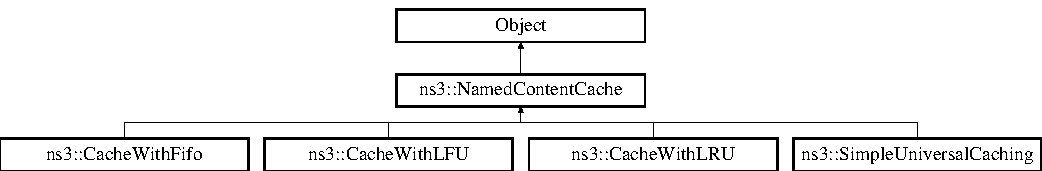
\includegraphics[height=2.295082cm]{classns3_1_1NamedContentCache}
\end{center}
\end{figure}
\subsection*{Public Types}
\begin{DoxyCompactItemize}
\item 
typedef boost\-::unordered\-\_\-map\\*
$<$ std\-::string, \\*
\hyperlink{classns3_1_1NamedContentCacheEntry}{Named\-Content\-Cache\-Entry} $>$ \hyperlink{classns3_1_1NamedContentCache_a9aa35d883b9f4153d97b6e7dc74f9307}{Cache}
\begin{DoxyCompactList}\small\item\em The main cache container which stores the data buffer and corresponding name is a boost\-::unordered\-\_\-map. This is because we don't need our cache entry to be sorted unnecessarily. \end{DoxyCompactList}\item 
typedef boost\-::bimap\\*
$<$ boost\-::bimaps\-::multiset\-\_\-of\\*
$<$ uint32\-\_\-t $>$\\*
, boost\-::bimaps\-::unordered\-\_\-set\-\_\-of\\*
$<$ std\-::string $>$ $>$ \hyperlink{classns3_1_1NamedContentCache_a0b728ea2d4e0acbe431897b2374cfc8e}{Policy\-Index}
\begin{DoxyCompactList}\small\item\em The indexed container which is necessary for the purpose of eviction based on caching policy, is a boost\-::bimap. A bimap is required because we'll be searching for both index and name for the purpose of eviction and updation respectively. \end{DoxyCompactList}\item 
typedef \\*
Policy\-Index\-::left\-\_\-map\-::iterator \hyperlink{classns3_1_1NamedContentCache_a0f52ee3d115d1b5fdd1201620b889b6e}{left\-\_\-iterator}
\begin{DoxyCompactList}\small\item\em Type Definition for the iterator of the left map of Policy\-Index. \end{DoxyCompactList}\item 
typedef \\*
Policy\-Index\-::right\-\_\-map\-::iterator \hyperlink{classns3_1_1NamedContentCache_a2c391c6013b29596a2ec5c62d0e413ed}{right\-\_\-iterator}
\begin{DoxyCompactList}\small\item\em Type Definition for the iterator of the right map of Policy\-Index. \end{DoxyCompactList}\item 
typedef \\*
Policy\-Index\-::left\-\_\-map\-::const\-\_\-iterator \hyperlink{classns3_1_1NamedContentCache_a061b957fbf37ee4eb873db49705bc388}{const\-\_\-left\-\_\-iterator}
\begin{DoxyCompactList}\small\item\em Type Definition for the constant iterator of the left map of Policy\-Index. \end{DoxyCompactList}\item 
typedef \\*
Policy\-Index\-::right\-\_\-map\-::const\-\_\-iterator \hyperlink{classns3_1_1NamedContentCache_a7489e77c6528954d887b8ff107a1244f}{const\-\_\-right\-\_\-iterator}
\begin{DoxyCompactList}\small\item\em Type Definition for the constant iterator of the right map of Policy\-Index. \end{DoxyCompactList}\end{DoxyCompactItemize}
\subsection*{Public Member Functions}
\begin{DoxyCompactItemize}
\item 
\hyperlink{classns3_1_1NamedContentCache_a4c6df9dacea268223c7a1cb9f17de93d}{Named\-Content\-Cache} ()
\item 
virtual \hyperlink{classns3_1_1NamedContentCache_a872f6440953cb44223b8584757f6bcfd}{$\sim$\-Named\-Content\-Cache} ()
\item 
virtual void \hyperlink{classns3_1_1NamedContentCache_ae28605a03a5a4d8b9a3494b4068f44e2}{Set\-Cache\-Size} (uint32\-\_\-t size)=0
\begin{DoxyCompactList}\small\item\em Set the cache size of the Cache. \end{DoxyCompactList}\item 
virtual uint32\-\_\-t \hyperlink{classns3_1_1NamedContentCache_afd9ade17d87082a46cbb745fd0196ab4}{Get\-Cache\-Size} (void)=0
\begin{DoxyCompactList}\small\item\em Get the cache size of the Cache. \end{DoxyCompactList}\item 
virtual void \hyperlink{classns3_1_1NamedContentCache_a92a5e2e641a11d15300f621aa77275ab}{Set\-Freshness\-Time} (uint64\-\_\-t time)=0
\begin{DoxyCompactList}\small\item\em Set the freshness time for the contents of Cache. \end{DoxyCompactList}\item 
virtual uint64\-\_\-t \hyperlink{classns3_1_1NamedContentCache_ac2b0e616d4e866cb2328e986f2ef69e1}{Get\-Freshness\-Time} (void)=0
\begin{DoxyCompactList}\small\item\em Get the freshness time set for the contents of Cache. \end{DoxyCompactList}\item 
virtual \hyperlink{classns3_1_1NamedContentCacheEntry}{Named\-Content\-Cache\-Entry} \hyperlink{classns3_1_1NamedContentCache_a154317526b3883db729c365ab342074a}{Create\-Entry} (std\-::string Name, Ptr$<$ Packet $>$ packet, Ipv4\-Header ipheader)=0
\begin{DoxyCompactList}\small\item\em Create the Cache entry, which is an object of \hyperlink{classns3_1_1NamedContentCacheEntry}{Named\-Content\-Cache\-Entry} class. The subclasses will define this function to create an entry that has the requisite parameters of the content, for the purpose of indexing content according to caching policy the subclass represents. \end{DoxyCompactList}\item 
virtual uint32\-\_\-t \hyperlink{classns3_1_1NamedContentCache_a75be49c2ad5db93bdf8aaed813dcf304}{Create\-Index} (\hyperlink{classns3_1_1NamedContentCacheEntry}{Named\-Content\-Cache\-Entry} entry)=0
\begin{DoxyCompactList}\small\item\em Create the index of the corresponding entry, by using the parameters of the content present in the entry class. The subclasses will define this function to create an index which, when put in order, will arrange the contents according to the caching policy the subclass represents. If some subclasses need decimal indexes, they have to multiply the obtained index with a factor to ensure unique integer indexes are obtained. \end{DoxyCompactList}\item 
virtual void \hyperlink{classns3_1_1NamedContentCache_a56a23add9b5bc03908793cf261ccb5f8}{Insert\-To\-Cache} (std\-::string Name, \hyperlink{classns3_1_1NamedContentCacheEntry}{Named\-Content\-Cache\-Entry} entry)=0
\begin{DoxyCompactList}\small\item\em Insert the Name of the content and its corresponding entry object to the Cache. \end{DoxyCompactList}\item 
virtual void \hyperlink{classns3_1_1NamedContentCache_ac248e647f56a6fef10285b1c654b8180}{Insert\-To\-Policy\-Index} (uint32\-\_\-t index, std\-::string Name)=0
\begin{DoxyCompactList}\small\item\em Insert the index of the content and its corresponding name to the Policy\-Index. \end{DoxyCompactList}\item 
virtual bool \hyperlink{classns3_1_1NamedContentCache_a1ceeaf5b85d3571225adfe2d48caf126}{Is\-Full} (void)=0
\begin{DoxyCompactList}\small\item\em Check if the Cache is full, i.\-e. if the number of contents is equal the cache size. \end{DoxyCompactList}\item 
virtual bool \hyperlink{classns3_1_1NamedContentCache_a4c4a79310c99f9c8ad6227d3b380dc20}{Is\-Unique} (std\-::string name)=0
\begin{DoxyCompactList}\small\item\em it check whether content is present in the cache or not \end{DoxyCompactList}\item 
virtual bool \hyperlink{classns3_1_1NamedContentCache_a281ad340f9771fa2ed898a1ad569d0da}{Is\-Evictable} (uint32\-\_\-t index)=0
\begin{DoxyCompactList}\small\item\em Check if the content with the given index can be inserted with the eviction of some other content when the is full. The new content can be inserted if its index is lesser than (or greater than, when arranged in descending order) the first content, or if any content's freshness has expired. Some caching policies, like F\-I\-F\-O, keep on inserting new content, irrespective of its index. Subclasses representing such policies need not define and use this function. \end{DoxyCompactList}\item 
virtual std\-::string \hyperlink{classns3_1_1NamedContentCache_a87850f01fc632ede64af75d7c20f7a7e}{Evict\-Entry} (void)=0
\begin{DoxyCompactList}\small\item\em Evict the first content in Policy\-Index and also the corresponding entry in the Cache. This is the main eviction function of \hyperlink{classns3_1_1NamedContentCache}{Named\-Content\-Cache}. \end{DoxyCompactList}\item 
virtual void \hyperlink{classns3_1_1NamedContentCache_a254f3c74475e104a615739fc7577296f}{Evict\-Entry} (std\-::string Name)=0
\begin{DoxyCompactList}\small\item\em Evict the content with corresponding name from both Policy\-Index and Cache. This has to be done when a packet having a content that already exists in the Cache has been received the I\-C\-N Router. This operation basically evicts the older entry of the same content so that the newer entry can be inserted. This function has to be defined by all subclasses because every content name in Cache and Policy\-Index has to be unique. \end{DoxyCompactList}\item 
virtual Ptr$<$ Packet $>$ \hyperlink{classns3_1_1NamedContentCache_a081439cd96d09e2f9f158f3aebe9fd7c}{Find} (std\-::string Name)=0
\begin{DoxyCompactList}\small\item\em Find the content with given name in the Cache. \end{DoxyCompactList}\item 
virtual void \hyperlink{classns3_1_1NamedContentCache_aeabf8afacd89cbc46b78b382c8a487e8}{Update\-Index} (std\-::string Name)=0
\begin{DoxyCompactList}\small\item\em Update the index of the content with the given name. This has to be done when the content is retrieved from Cache to be sent to a querying O\-I\-C\-N Client. The subclasses will define this function based on the requirements of the caching policies they represent. \end{DoxyCompactList}\end{DoxyCompactItemize}
\subsection*{Static Public Member Functions}
\begin{DoxyCompactItemize}
\item 
static Type\-Id \hyperlink{classns3_1_1NamedContentCache_a6e1837a2d8896d7a53c7a8b1d3a472d3}{Get\-Type\-Id} (void)
\begin{DoxyCompactList}\small\item\em Get the type I\-D. \end{DoxyCompactList}\end{DoxyCompactItemize}


\subsection{Detailed Description}
The base class for caching data at the I\-C\-N Router. 

This class is a base class for all different types of I\-C\-N Router cache, i.\-e. a F\-I\-F\-O based cache, an L\-R\-U based cache, a customized cache etc. This class provides the two essential containers required for a typical cache, a container to store the actual data, called Cache, and a container to store the index of the corresponding data, called Policy\-Index.

A Cache entry is an object of \hyperlink{classns3_1_1NamedContentCacheEntry}{Named\-Content\-Cache\-Entry} class, which is basically a struct containing the data along with various parameters corresponding to data, like timestamp, source I\-P etc. More about \hyperlink{classns3_1_1NamedContentCacheEntry}{Named\-Content\-Cache\-Entry} class can be found in its header file.

Depending on caching policy used by a particular subclass, the index of a content is calculated using the required parameters present in the cache entry. The \hyperlink{classns3_1_1NamedContentCache}{Named\-Content\-Cache} class basically contains the declarations for all required virtual functions needed for handling a cache, i.\-e. insertion, eviction etc.

This class is instantiated and aggregated to all I\-C\-N Routers in the network, and is not required in any other components of O\-I\-C\-N Architecture.

Note\-: The word Cache here refers to the boost\-::unordered\-\_\-map that stores the content along with its corresponding name. The word Policy\-Index refers to the boost\-::bimap container used for indexing the stored content in Cache. 

\subsection{Member Typedef Documentation}
\hypertarget{classns3_1_1NamedContentCache_a9aa35d883b9f4153d97b6e7dc74f9307}{\index{ns3\-::\-Named\-Content\-Cache@{ns3\-::\-Named\-Content\-Cache}!Cache@{Cache}}
\index{Cache@{Cache}!ns3::NamedContentCache@{ns3\-::\-Named\-Content\-Cache}}
\subsubsection[{Cache}]{\setlength{\rightskip}{0pt plus 5cm}typedef boost\-::unordered\-\_\-map$<$std\-::string, {\bf Named\-Content\-Cache\-Entry}$>$ {\bf ns3\-::\-Named\-Content\-Cache\-::\-Cache}}}\label{classns3_1_1NamedContentCache_a9aa35d883b9f4153d97b6e7dc74f9307}


The main cache container which stores the data buffer and corresponding name is a boost\-::unordered\-\_\-map. This is because we don't need our cache entry to be sorted unnecessarily. 

\hypertarget{classns3_1_1NamedContentCache_a061b957fbf37ee4eb873db49705bc388}{\index{ns3\-::\-Named\-Content\-Cache@{ns3\-::\-Named\-Content\-Cache}!const\-\_\-left\-\_\-iterator@{const\-\_\-left\-\_\-iterator}}
\index{const\-\_\-left\-\_\-iterator@{const\-\_\-left\-\_\-iterator}!ns3::NamedContentCache@{ns3\-::\-Named\-Content\-Cache}}
\subsubsection[{const\-\_\-left\-\_\-iterator}]{\setlength{\rightskip}{0pt plus 5cm}typedef Policy\-Index\-::left\-\_\-map\-::const\-\_\-iterator {\bf ns3\-::\-Named\-Content\-Cache\-::const\-\_\-left\-\_\-iterator}}}\label{classns3_1_1NamedContentCache_a061b957fbf37ee4eb873db49705bc388}


Type Definition for the constant iterator of the left map of Policy\-Index. 

\hypertarget{classns3_1_1NamedContentCache_a7489e77c6528954d887b8ff107a1244f}{\index{ns3\-::\-Named\-Content\-Cache@{ns3\-::\-Named\-Content\-Cache}!const\-\_\-right\-\_\-iterator@{const\-\_\-right\-\_\-iterator}}
\index{const\-\_\-right\-\_\-iterator@{const\-\_\-right\-\_\-iterator}!ns3::NamedContentCache@{ns3\-::\-Named\-Content\-Cache}}
\subsubsection[{const\-\_\-right\-\_\-iterator}]{\setlength{\rightskip}{0pt plus 5cm}typedef Policy\-Index\-::right\-\_\-map\-::const\-\_\-iterator {\bf ns3\-::\-Named\-Content\-Cache\-::const\-\_\-right\-\_\-iterator}}}\label{classns3_1_1NamedContentCache_a7489e77c6528954d887b8ff107a1244f}


Type Definition for the constant iterator of the right map of Policy\-Index. 

\hypertarget{classns3_1_1NamedContentCache_a0f52ee3d115d1b5fdd1201620b889b6e}{\index{ns3\-::\-Named\-Content\-Cache@{ns3\-::\-Named\-Content\-Cache}!left\-\_\-iterator@{left\-\_\-iterator}}
\index{left\-\_\-iterator@{left\-\_\-iterator}!ns3::NamedContentCache@{ns3\-::\-Named\-Content\-Cache}}
\subsubsection[{left\-\_\-iterator}]{\setlength{\rightskip}{0pt plus 5cm}typedef Policy\-Index\-::left\-\_\-map\-::iterator {\bf ns3\-::\-Named\-Content\-Cache\-::left\-\_\-iterator}}}\label{classns3_1_1NamedContentCache_a0f52ee3d115d1b5fdd1201620b889b6e}


Type Definition for the iterator of the left map of Policy\-Index. 

\hypertarget{classns3_1_1NamedContentCache_a0b728ea2d4e0acbe431897b2374cfc8e}{\index{ns3\-::\-Named\-Content\-Cache@{ns3\-::\-Named\-Content\-Cache}!Policy\-Index@{Policy\-Index}}
\index{Policy\-Index@{Policy\-Index}!ns3::NamedContentCache@{ns3\-::\-Named\-Content\-Cache}}
\subsubsection[{Policy\-Index}]{\setlength{\rightskip}{0pt plus 5cm}typedef boost\-::bimap$<$boost\-::bimaps\-::multiset\-\_\-of$<$uint32\-\_\-t$>$, boost\-::bimaps\-::unordered\-\_\-set\-\_\-of$<$std\-::string$>$ $>$ {\bf ns3\-::\-Named\-Content\-Cache\-::\-Policy\-Index}}}\label{classns3_1_1NamedContentCache_a0b728ea2d4e0acbe431897b2374cfc8e}


The indexed container which is necessary for the purpose of eviction based on caching policy, is a boost\-::bimap. A bimap is required because we'll be searching for both index and name for the purpose of eviction and updation respectively. 

\hypertarget{classns3_1_1NamedContentCache_a2c391c6013b29596a2ec5c62d0e413ed}{\index{ns3\-::\-Named\-Content\-Cache@{ns3\-::\-Named\-Content\-Cache}!right\-\_\-iterator@{right\-\_\-iterator}}
\index{right\-\_\-iterator@{right\-\_\-iterator}!ns3::NamedContentCache@{ns3\-::\-Named\-Content\-Cache}}
\subsubsection[{right\-\_\-iterator}]{\setlength{\rightskip}{0pt plus 5cm}typedef Policy\-Index\-::right\-\_\-map\-::iterator {\bf ns3\-::\-Named\-Content\-Cache\-::right\-\_\-iterator}}}\label{classns3_1_1NamedContentCache_a2c391c6013b29596a2ec5c62d0e413ed}


Type Definition for the iterator of the right map of Policy\-Index. 



\subsection{Constructor \& Destructor Documentation}
\hypertarget{classns3_1_1NamedContentCache_a4c6df9dacea268223c7a1cb9f17de93d}{\index{ns3\-::\-Named\-Content\-Cache@{ns3\-::\-Named\-Content\-Cache}!Named\-Content\-Cache@{Named\-Content\-Cache}}
\index{Named\-Content\-Cache@{Named\-Content\-Cache}!ns3::NamedContentCache@{ns3\-::\-Named\-Content\-Cache}}
\subsubsection[{Named\-Content\-Cache}]{\setlength{\rightskip}{0pt plus 5cm}ns3\-::\-Named\-Content\-Cache\-::\-Named\-Content\-Cache (
\begin{DoxyParamCaption}
{}
\end{DoxyParamCaption}
)}}\label{classns3_1_1NamedContentCache_a4c6df9dacea268223c7a1cb9f17de93d}
\hypertarget{classns3_1_1NamedContentCache_a872f6440953cb44223b8584757f6bcfd}{\index{ns3\-::\-Named\-Content\-Cache@{ns3\-::\-Named\-Content\-Cache}!$\sim$\-Named\-Content\-Cache@{$\sim$\-Named\-Content\-Cache}}
\index{$\sim$\-Named\-Content\-Cache@{$\sim$\-Named\-Content\-Cache}!ns3::NamedContentCache@{ns3\-::\-Named\-Content\-Cache}}
\subsubsection[{$\sim$\-Named\-Content\-Cache}]{\setlength{\rightskip}{0pt plus 5cm}ns3\-::\-Named\-Content\-Cache\-::$\sim$\-Named\-Content\-Cache (
\begin{DoxyParamCaption}
{}
\end{DoxyParamCaption}
)\hspace{0.3cm}{\ttfamily [virtual]}}}\label{classns3_1_1NamedContentCache_a872f6440953cb44223b8584757f6bcfd}


\subsection{Member Function Documentation}
\hypertarget{classns3_1_1NamedContentCache_a154317526b3883db729c365ab342074a}{\index{ns3\-::\-Named\-Content\-Cache@{ns3\-::\-Named\-Content\-Cache}!Create\-Entry@{Create\-Entry}}
\index{Create\-Entry@{Create\-Entry}!ns3::NamedContentCache@{ns3\-::\-Named\-Content\-Cache}}
\subsubsection[{Create\-Entry}]{\setlength{\rightskip}{0pt plus 5cm}virtual {\bf Named\-Content\-Cache\-Entry} ns3\-::\-Named\-Content\-Cache\-::\-Create\-Entry (
\begin{DoxyParamCaption}
\item[{std\-::string}]{Name, }
\item[{Ptr$<$ Packet $>$}]{packet, }
\item[{Ipv4\-Header}]{ipheader}
\end{DoxyParamCaption}
)\hspace{0.3cm}{\ttfamily [pure virtual]}}}\label{classns3_1_1NamedContentCache_a154317526b3883db729c365ab342074a}


Create the Cache entry, which is an object of \hyperlink{classns3_1_1NamedContentCacheEntry}{Named\-Content\-Cache\-Entry} class. The subclasses will define this function to create an entry that has the requisite parameters of the content, for the purpose of indexing content according to caching policy the subclass represents. 


\begin{DoxyParams}{Parameters}
{\em Name} & name of the content \\
\hline
{\em packet} & packet received by I\-C\-N Router, with its I\-P, Transport and O\-I\-C\-N headers removed \\
\hline
{\em ipheader} & I\-P Header of the packet, from which the required parameters of the content (present in packet) can retrieved. \\
\hline
\end{DoxyParams}
\begin{DoxyReturn}{Returns}
the newly created cache entry 
\end{DoxyReturn}


Implemented in \hyperlink{classns3_1_1CacheWithLFU_a214a07a5f2af6c8532ee1a729d252f68}{ns3\-::\-Cache\-With\-L\-F\-U}, \hyperlink{classns3_1_1SimpleUniversalCaching_a95d289d9580f5af31885b8deb9738451}{ns3\-::\-Simple\-Universal\-Caching}, \hyperlink{classns3_1_1CacheWithLRU_a8dc721b8593047e5246b3ffa21c83ba2}{ns3\-::\-Cache\-With\-L\-R\-U}, and \hyperlink{classns3_1_1CacheWithFifo_ae9be9920ddca0d7a001a054381c0543c}{ns3\-::\-Cache\-With\-Fifo}.

\hypertarget{classns3_1_1NamedContentCache_a75be49c2ad5db93bdf8aaed813dcf304}{\index{ns3\-::\-Named\-Content\-Cache@{ns3\-::\-Named\-Content\-Cache}!Create\-Index@{Create\-Index}}
\index{Create\-Index@{Create\-Index}!ns3::NamedContentCache@{ns3\-::\-Named\-Content\-Cache}}
\subsubsection[{Create\-Index}]{\setlength{\rightskip}{0pt plus 5cm}virtual uint32\-\_\-t ns3\-::\-Named\-Content\-Cache\-::\-Create\-Index (
\begin{DoxyParamCaption}
\item[{{\bf Named\-Content\-Cache\-Entry}}]{entry}
\end{DoxyParamCaption}
)\hspace{0.3cm}{\ttfamily [pure virtual]}}}\label{classns3_1_1NamedContentCache_a75be49c2ad5db93bdf8aaed813dcf304}


Create the index of the corresponding entry, by using the parameters of the content present in the entry class. The subclasses will define this function to create an index which, when put in order, will arrange the contents according to the caching policy the subclass represents. If some subclasses need decimal indexes, they have to multiply the obtained index with a factor to ensure unique integer indexes are obtained. 


\begin{DoxyParams}{Parameters}
{\em entry} & the cache entry corresponding to the content \\
\hline
\end{DoxyParams}
\begin{DoxyReturn}{Returns}
the newly created integer index for the content 
\end{DoxyReturn}


Implemented in \hyperlink{classns3_1_1CacheWithLFU_a8c1c53863063d36a20aab3e643301119}{ns3\-::\-Cache\-With\-L\-F\-U}, \hyperlink{classns3_1_1SimpleUniversalCaching_aeec1f45196ce8ffe82baf2439e4ee064}{ns3\-::\-Simple\-Universal\-Caching}, \hyperlink{classns3_1_1CacheWithLRU_a5129171c03d524afe292aec079397d40}{ns3\-::\-Cache\-With\-L\-R\-U}, and \hyperlink{classns3_1_1CacheWithFifo_a15c2b5cf0e52e8da5fbd4d7e32d0aedc}{ns3\-::\-Cache\-With\-Fifo}.

\hypertarget{classns3_1_1NamedContentCache_a87850f01fc632ede64af75d7c20f7a7e}{\index{ns3\-::\-Named\-Content\-Cache@{ns3\-::\-Named\-Content\-Cache}!Evict\-Entry@{Evict\-Entry}}
\index{Evict\-Entry@{Evict\-Entry}!ns3::NamedContentCache@{ns3\-::\-Named\-Content\-Cache}}
\subsubsection[{Evict\-Entry}]{\setlength{\rightskip}{0pt plus 5cm}virtual std\-::string ns3\-::\-Named\-Content\-Cache\-::\-Evict\-Entry (
\begin{DoxyParamCaption}
\item[{void}]{}
\end{DoxyParamCaption}
)\hspace{0.3cm}{\ttfamily [pure virtual]}}}\label{classns3_1_1NamedContentCache_a87850f01fc632ede64af75d7c20f7a7e}


Evict the first content in Policy\-Index and also the corresponding entry in the Cache. This is the main eviction function of \hyperlink{classns3_1_1NamedContentCache}{Named\-Content\-Cache}. 

\begin{DoxyReturn}{Returns}
the name of the evicted content 
\end{DoxyReturn}


Implemented in \hyperlink{classns3_1_1CacheWithLFU_a9dda5e2a61f82f7eaa2121a2de2f5a8f}{ns3\-::\-Cache\-With\-L\-F\-U}, \hyperlink{classns3_1_1SimpleUniversalCaching_a2055b9586523ae15979da923dfac65fc}{ns3\-::\-Simple\-Universal\-Caching}, \hyperlink{classns3_1_1CacheWithLRU_a657627f6ab6b395086c44bf7e51063fc}{ns3\-::\-Cache\-With\-L\-R\-U}, and \hyperlink{classns3_1_1CacheWithFifo_a3440b3cf70e24dd33d511656c0d77112}{ns3\-::\-Cache\-With\-Fifo}.

\hypertarget{classns3_1_1NamedContentCache_a254f3c74475e104a615739fc7577296f}{\index{ns3\-::\-Named\-Content\-Cache@{ns3\-::\-Named\-Content\-Cache}!Evict\-Entry@{Evict\-Entry}}
\index{Evict\-Entry@{Evict\-Entry}!ns3::NamedContentCache@{ns3\-::\-Named\-Content\-Cache}}
\subsubsection[{Evict\-Entry}]{\setlength{\rightskip}{0pt plus 5cm}virtual void ns3\-::\-Named\-Content\-Cache\-::\-Evict\-Entry (
\begin{DoxyParamCaption}
\item[{std\-::string}]{Name}
\end{DoxyParamCaption}
)\hspace{0.3cm}{\ttfamily [pure virtual]}}}\label{classns3_1_1NamedContentCache_a254f3c74475e104a615739fc7577296f}


Evict the content with corresponding name from both Policy\-Index and Cache. This has to be done when a packet having a content that already exists in the Cache has been received the I\-C\-N Router. This operation basically evicts the older entry of the same content so that the newer entry can be inserted. This function has to be defined by all subclasses because every content name in Cache and Policy\-Index has to be unique. 


\begin{DoxyParams}{Parameters}
{\em name} & name of the non-\/unique content \\
\hline
\end{DoxyParams}


Implemented in \hyperlink{classns3_1_1CacheWithLFU_aa04d4be1c2ea84020f5eac561a8ebe22}{ns3\-::\-Cache\-With\-L\-F\-U}, \hyperlink{classns3_1_1SimpleUniversalCaching_a1913c0525f12b726eb04567bb3254551}{ns3\-::\-Simple\-Universal\-Caching}, \hyperlink{classns3_1_1CacheWithLRU_abd2898e58b7eeb214153a29379e05404}{ns3\-::\-Cache\-With\-L\-R\-U}, and \hyperlink{classns3_1_1CacheWithFifo_a156013f129c1d13538ed92e6116a2d20}{ns3\-::\-Cache\-With\-Fifo}.

\hypertarget{classns3_1_1NamedContentCache_a081439cd96d09e2f9f158f3aebe9fd7c}{\index{ns3\-::\-Named\-Content\-Cache@{ns3\-::\-Named\-Content\-Cache}!Find@{Find}}
\index{Find@{Find}!ns3::NamedContentCache@{ns3\-::\-Named\-Content\-Cache}}
\subsubsection[{Find}]{\setlength{\rightskip}{0pt plus 5cm}virtual Ptr$<$Packet$>$ ns3\-::\-Named\-Content\-Cache\-::\-Find (
\begin{DoxyParamCaption}
\item[{std\-::string}]{Name}
\end{DoxyParamCaption}
)\hspace{0.3cm}{\ttfamily [pure virtual]}}}\label{classns3_1_1NamedContentCache_a081439cd96d09e2f9f158f3aebe9fd7c}


Find the content with given name in the Cache. 

\begin{DoxyReturn}{Returns}
the content in the form of an Application Layer packet 
\end{DoxyReturn}


Implemented in \hyperlink{classns3_1_1CacheWithLFU_af36841e8b113ed62ad8827785fa03740}{ns3\-::\-Cache\-With\-L\-F\-U}, \hyperlink{classns3_1_1SimpleUniversalCaching_a492b9405dff0ced8bae565bc98f5361c}{ns3\-::\-Simple\-Universal\-Caching}, \hyperlink{classns3_1_1CacheWithLRU_a2948736630124fd3a5efcdc69ac04126}{ns3\-::\-Cache\-With\-L\-R\-U}, and \hyperlink{classns3_1_1CacheWithFifo_a36311448f4cef69aa4be77dfc91eb3d5}{ns3\-::\-Cache\-With\-Fifo}.

\hypertarget{classns3_1_1NamedContentCache_afd9ade17d87082a46cbb745fd0196ab4}{\index{ns3\-::\-Named\-Content\-Cache@{ns3\-::\-Named\-Content\-Cache}!Get\-Cache\-Size@{Get\-Cache\-Size}}
\index{Get\-Cache\-Size@{Get\-Cache\-Size}!ns3::NamedContentCache@{ns3\-::\-Named\-Content\-Cache}}
\subsubsection[{Get\-Cache\-Size}]{\setlength{\rightskip}{0pt plus 5cm}virtual uint32\-\_\-t ns3\-::\-Named\-Content\-Cache\-::\-Get\-Cache\-Size (
\begin{DoxyParamCaption}
\item[{void}]{}
\end{DoxyParamCaption}
)\hspace{0.3cm}{\ttfamily [pure virtual]}}}\label{classns3_1_1NamedContentCache_afd9ade17d87082a46cbb745fd0196ab4}


Get the cache size of the Cache. 

\begin{DoxyReturn}{Returns}
the cache size of the Cache 
\end{DoxyReturn}


Implemented in \hyperlink{classns3_1_1CacheWithLFU_a2d58ee7990ca6ecf0db3fea70bdc09ef}{ns3\-::\-Cache\-With\-L\-F\-U}, \hyperlink{classns3_1_1SimpleUniversalCaching_a923d1d730c8d0171e2366773b950d165}{ns3\-::\-Simple\-Universal\-Caching}, \hyperlink{classns3_1_1CacheWithLRU_a7011075202d46dc23358058ed8037125}{ns3\-::\-Cache\-With\-L\-R\-U}, and \hyperlink{classns3_1_1CacheWithFifo_ae94f385620f20825ad07995dccc8075a}{ns3\-::\-Cache\-With\-Fifo}.

\hypertarget{classns3_1_1NamedContentCache_ac2b0e616d4e866cb2328e986f2ef69e1}{\index{ns3\-::\-Named\-Content\-Cache@{ns3\-::\-Named\-Content\-Cache}!Get\-Freshness\-Time@{Get\-Freshness\-Time}}
\index{Get\-Freshness\-Time@{Get\-Freshness\-Time}!ns3::NamedContentCache@{ns3\-::\-Named\-Content\-Cache}}
\subsubsection[{Get\-Freshness\-Time}]{\setlength{\rightskip}{0pt plus 5cm}virtual uint64\-\_\-t ns3\-::\-Named\-Content\-Cache\-::\-Get\-Freshness\-Time (
\begin{DoxyParamCaption}
\item[{void}]{}
\end{DoxyParamCaption}
)\hspace{0.3cm}{\ttfamily [pure virtual]}}}\label{classns3_1_1NamedContentCache_ac2b0e616d4e866cb2328e986f2ef69e1}


Get the freshness time set for the contents of Cache. 

\begin{DoxyReturn}{Returns}
the freshness time in milliseconds 
\end{DoxyReturn}


Implemented in \hyperlink{classns3_1_1CacheWithLFU_a27a3e1d0b4b308a51ccf58dce5df9bee}{ns3\-::\-Cache\-With\-L\-F\-U}, \hyperlink{classns3_1_1SimpleUniversalCaching_a164cda8301046d0123443419528c6b3e}{ns3\-::\-Simple\-Universal\-Caching}, \hyperlink{classns3_1_1CacheWithLRU_ad3f0a3b34a506792f30310761242a86c}{ns3\-::\-Cache\-With\-L\-R\-U}, and \hyperlink{classns3_1_1CacheWithFifo_aa56864aee34859897793284eb7c7f9db}{ns3\-::\-Cache\-With\-Fifo}.

\hypertarget{classns3_1_1NamedContentCache_a6e1837a2d8896d7a53c7a8b1d3a472d3}{\index{ns3\-::\-Named\-Content\-Cache@{ns3\-::\-Named\-Content\-Cache}!Get\-Type\-Id@{Get\-Type\-Id}}
\index{Get\-Type\-Id@{Get\-Type\-Id}!ns3::NamedContentCache@{ns3\-::\-Named\-Content\-Cache}}
\subsubsection[{Get\-Type\-Id}]{\setlength{\rightskip}{0pt plus 5cm}Type\-Id ns3\-::\-Named\-Content\-Cache\-::\-Get\-Type\-Id (
\begin{DoxyParamCaption}
\item[{void}]{}
\end{DoxyParamCaption}
)\hspace{0.3cm}{\ttfamily [static]}}}\label{classns3_1_1NamedContentCache_a6e1837a2d8896d7a53c7a8b1d3a472d3}


Get the type I\-D. 

\begin{DoxyReturn}{Returns}
the object Type\-Id 
\end{DoxyReturn}
\hypertarget{classns3_1_1NamedContentCache_a56a23add9b5bc03908793cf261ccb5f8}{\index{ns3\-::\-Named\-Content\-Cache@{ns3\-::\-Named\-Content\-Cache}!Insert\-To\-Cache@{Insert\-To\-Cache}}
\index{Insert\-To\-Cache@{Insert\-To\-Cache}!ns3::NamedContentCache@{ns3\-::\-Named\-Content\-Cache}}
\subsubsection[{Insert\-To\-Cache}]{\setlength{\rightskip}{0pt plus 5cm}virtual void ns3\-::\-Named\-Content\-Cache\-::\-Insert\-To\-Cache (
\begin{DoxyParamCaption}
\item[{std\-::string}]{Name, }
\item[{{\bf Named\-Content\-Cache\-Entry}}]{entry}
\end{DoxyParamCaption}
)\hspace{0.3cm}{\ttfamily [pure virtual]}}}\label{classns3_1_1NamedContentCache_a56a23add9b5bc03908793cf261ccb5f8}


Insert the Name of the content and its corresponding entry object to the Cache. 


\begin{DoxyParams}{Parameters}
{\em Name} & name of the content \\
\hline
{\em entry} & the cache entry corresponding to the content \\
\hline
\end{DoxyParams}


Implemented in \hyperlink{classns3_1_1CacheWithLFU_a85d1afb801554e39390c07d07d33d5e7}{ns3\-::\-Cache\-With\-L\-F\-U}, \hyperlink{classns3_1_1SimpleUniversalCaching_a18713ba18ecbf1ef06b0efdf2ef3d83b}{ns3\-::\-Simple\-Universal\-Caching}, \hyperlink{classns3_1_1CacheWithLRU_adfce286e921a3f3d4cbf9e1008cae632}{ns3\-::\-Cache\-With\-L\-R\-U}, and \hyperlink{classns3_1_1CacheWithFifo_a2b0a3e5d4d83775f99e6a453bbb9f764}{ns3\-::\-Cache\-With\-Fifo}.

\hypertarget{classns3_1_1NamedContentCache_ac248e647f56a6fef10285b1c654b8180}{\index{ns3\-::\-Named\-Content\-Cache@{ns3\-::\-Named\-Content\-Cache}!Insert\-To\-Policy\-Index@{Insert\-To\-Policy\-Index}}
\index{Insert\-To\-Policy\-Index@{Insert\-To\-Policy\-Index}!ns3::NamedContentCache@{ns3\-::\-Named\-Content\-Cache}}
\subsubsection[{Insert\-To\-Policy\-Index}]{\setlength{\rightskip}{0pt plus 5cm}virtual void ns3\-::\-Named\-Content\-Cache\-::\-Insert\-To\-Policy\-Index (
\begin{DoxyParamCaption}
\item[{uint32\-\_\-t}]{index, }
\item[{std\-::string}]{Name}
\end{DoxyParamCaption}
)\hspace{0.3cm}{\ttfamily [pure virtual]}}}\label{classns3_1_1NamedContentCache_ac248e647f56a6fef10285b1c654b8180}


Insert the index of the content and its corresponding name to the Policy\-Index. 


\begin{DoxyParams}{Parameters}
{\em index} & the unique integer index of the content \\
\hline
{\em Name} & name of the content \\
\hline
\end{DoxyParams}


Implemented in \hyperlink{classns3_1_1CacheWithLFU_a5741df65535e31319d6d534ff1f8aa2f}{ns3\-::\-Cache\-With\-L\-F\-U}, \hyperlink{classns3_1_1SimpleUniversalCaching_aaeed7c05fc53f6bcb667057b72bfd718}{ns3\-::\-Simple\-Universal\-Caching}, \hyperlink{classns3_1_1CacheWithLRU_a8b5e0eb51220cba226f913ddc1ef304f}{ns3\-::\-Cache\-With\-L\-R\-U}, and \hyperlink{classns3_1_1CacheWithFifo_a2f6375a96e425628f4ef48df89fc2319}{ns3\-::\-Cache\-With\-Fifo}.

\hypertarget{classns3_1_1NamedContentCache_a281ad340f9771fa2ed898a1ad569d0da}{\index{ns3\-::\-Named\-Content\-Cache@{ns3\-::\-Named\-Content\-Cache}!Is\-Evictable@{Is\-Evictable}}
\index{Is\-Evictable@{Is\-Evictable}!ns3::NamedContentCache@{ns3\-::\-Named\-Content\-Cache}}
\subsubsection[{Is\-Evictable}]{\setlength{\rightskip}{0pt plus 5cm}virtual bool ns3\-::\-Named\-Content\-Cache\-::\-Is\-Evictable (
\begin{DoxyParamCaption}
\item[{uint32\-\_\-t}]{index}
\end{DoxyParamCaption}
)\hspace{0.3cm}{\ttfamily [pure virtual]}}}\label{classns3_1_1NamedContentCache_a281ad340f9771fa2ed898a1ad569d0da}


Check if the content with the given index can be inserted with the eviction of some other content when the is full. The new content can be inserted if its index is lesser than (or greater than, when arranged in descending order) the first content, or if any content's freshness has expired. Some caching policies, like F\-I\-F\-O, keep on inserting new content, irrespective of its index. Subclasses representing such policies need not define and use this function. 


\begin{DoxyParams}{Parameters}
{\em index} & the unique integer index of the content \\
\hline
\end{DoxyParams}
\begin{DoxyReturn}{Returns}
true if any existing content can be evicted so that the new content with the given index can be inserted. 
\end{DoxyReturn}


Implemented in \hyperlink{classns3_1_1CacheWithLFU_a4ac9bfbe6e1b12952c345051517b762f}{ns3\-::\-Cache\-With\-L\-F\-U}, \hyperlink{classns3_1_1SimpleUniversalCaching_a2aaf1a6027c2c635a1c74a7ca279970f}{ns3\-::\-Simple\-Universal\-Caching}, \hyperlink{classns3_1_1CacheWithLRU_a29fae4efb96e97023459866634488a28}{ns3\-::\-Cache\-With\-L\-R\-U}, and \hyperlink{classns3_1_1CacheWithFifo_a69b633b7e17cb8f13e7a66afb942a258}{ns3\-::\-Cache\-With\-Fifo}.

\hypertarget{classns3_1_1NamedContentCache_a1ceeaf5b85d3571225adfe2d48caf126}{\index{ns3\-::\-Named\-Content\-Cache@{ns3\-::\-Named\-Content\-Cache}!Is\-Full@{Is\-Full}}
\index{Is\-Full@{Is\-Full}!ns3::NamedContentCache@{ns3\-::\-Named\-Content\-Cache}}
\subsubsection[{Is\-Full}]{\setlength{\rightskip}{0pt plus 5cm}virtual bool ns3\-::\-Named\-Content\-Cache\-::\-Is\-Full (
\begin{DoxyParamCaption}
\item[{void}]{}
\end{DoxyParamCaption}
)\hspace{0.3cm}{\ttfamily [pure virtual]}}}\label{classns3_1_1NamedContentCache_a1ceeaf5b85d3571225adfe2d48caf126}


Check if the Cache is full, i.\-e. if the number of contents is equal the cache size. 

\begin{DoxyReturn}{Returns}
true if the Cache is full 
\end{DoxyReturn}


Implemented in \hyperlink{classns3_1_1CacheWithLFU_a791ed7f4bebc707e18852e346f536bd8}{ns3\-::\-Cache\-With\-L\-F\-U}, \hyperlink{classns3_1_1SimpleUniversalCaching_ab28cafb9e7ea79d7a318d7cafa7293f7}{ns3\-::\-Simple\-Universal\-Caching}, \hyperlink{classns3_1_1CacheWithLRU_ac8cea24f840cdfb15abb1f09638b0fb1}{ns3\-::\-Cache\-With\-L\-R\-U}, and \hyperlink{classns3_1_1CacheWithFifo_a15468a5d2fc215b32a8e531944c4197e}{ns3\-::\-Cache\-With\-Fifo}.

\hypertarget{classns3_1_1NamedContentCache_a4c4a79310c99f9c8ad6227d3b380dc20}{\index{ns3\-::\-Named\-Content\-Cache@{ns3\-::\-Named\-Content\-Cache}!Is\-Unique@{Is\-Unique}}
\index{Is\-Unique@{Is\-Unique}!ns3::NamedContentCache@{ns3\-::\-Named\-Content\-Cache}}
\subsubsection[{Is\-Unique}]{\setlength{\rightskip}{0pt plus 5cm}virtual bool ns3\-::\-Named\-Content\-Cache\-::\-Is\-Unique (
\begin{DoxyParamCaption}
\item[{std\-::string}]{name}
\end{DoxyParamCaption}
)\hspace{0.3cm}{\ttfamily [pure virtual]}}}\label{classns3_1_1NamedContentCache_a4c4a79310c99f9c8ad6227d3b380dc20}


it check whether content is present in the cache or not 


\begin{DoxyParams}{Parameters}
{\em name} & name of the content \\
\hline
\end{DoxyParams}
\begin{DoxyReturn}{Returns}
true if content is not present, false when content is present in the cache 
\end{DoxyReturn}


Implemented in \hyperlink{classns3_1_1CacheWithLFU_a4999cd730f44907c1fdf3f8ea11f4de1}{ns3\-::\-Cache\-With\-L\-F\-U}, \hyperlink{classns3_1_1SimpleUniversalCaching_a3f334cfd08d2a1dbbee280cde3d7fe22}{ns3\-::\-Simple\-Universal\-Caching}, \hyperlink{classns3_1_1CacheWithLRU_a8c69352212c41da32499d84add8dd42d}{ns3\-::\-Cache\-With\-L\-R\-U}, and \hyperlink{classns3_1_1CacheWithFifo_a90d9c0afe3ef2579dd6faf1f70aeb4e0}{ns3\-::\-Cache\-With\-Fifo}.

\hypertarget{classns3_1_1NamedContentCache_ae28605a03a5a4d8b9a3494b4068f44e2}{\index{ns3\-::\-Named\-Content\-Cache@{ns3\-::\-Named\-Content\-Cache}!Set\-Cache\-Size@{Set\-Cache\-Size}}
\index{Set\-Cache\-Size@{Set\-Cache\-Size}!ns3::NamedContentCache@{ns3\-::\-Named\-Content\-Cache}}
\subsubsection[{Set\-Cache\-Size}]{\setlength{\rightskip}{0pt plus 5cm}virtual void ns3\-::\-Named\-Content\-Cache\-::\-Set\-Cache\-Size (
\begin{DoxyParamCaption}
\item[{uint32\-\_\-t}]{size}
\end{DoxyParamCaption}
)\hspace{0.3cm}{\ttfamily [pure virtual]}}}\label{classns3_1_1NamedContentCache_ae28605a03a5a4d8b9a3494b4068f44e2}


Set the cache size of the Cache. 


\begin{DoxyParams}{Parameters}
{\em size} & the size to which the cache has to be set \\
\hline
\end{DoxyParams}


Implemented in \hyperlink{classns3_1_1CacheWithLFU_a80bda10cdbc2edca79e6efe8e4fac60e}{ns3\-::\-Cache\-With\-L\-F\-U}, \hyperlink{classns3_1_1SimpleUniversalCaching_aa6123b2df8e357e30b84edf190d874c8}{ns3\-::\-Simple\-Universal\-Caching}, \hyperlink{classns3_1_1CacheWithLRU_a75323b8c1d45dbaa19e07bf6fdf9b9a3}{ns3\-::\-Cache\-With\-L\-R\-U}, and \hyperlink{classns3_1_1CacheWithFifo_a6e92a91f36ac87a001644e299be4dd41}{ns3\-::\-Cache\-With\-Fifo}.

\hypertarget{classns3_1_1NamedContentCache_a92a5e2e641a11d15300f621aa77275ab}{\index{ns3\-::\-Named\-Content\-Cache@{ns3\-::\-Named\-Content\-Cache}!Set\-Freshness\-Time@{Set\-Freshness\-Time}}
\index{Set\-Freshness\-Time@{Set\-Freshness\-Time}!ns3::NamedContentCache@{ns3\-::\-Named\-Content\-Cache}}
\subsubsection[{Set\-Freshness\-Time}]{\setlength{\rightskip}{0pt plus 5cm}virtual void ns3\-::\-Named\-Content\-Cache\-::\-Set\-Freshness\-Time (
\begin{DoxyParamCaption}
\item[{uint64\-\_\-t}]{time}
\end{DoxyParamCaption}
)\hspace{0.3cm}{\ttfamily [pure virtual]}}}\label{classns3_1_1NamedContentCache_a92a5e2e641a11d15300f621aa77275ab}


Set the freshness time for the contents of Cache. 


\begin{DoxyParams}{Parameters}
{\em time} & the freshness time in milliseconds \\
\hline
\end{DoxyParams}


Implemented in \hyperlink{classns3_1_1CacheWithLFU_a3f5fc35d85cee3f4b405ccabd977662b}{ns3\-::\-Cache\-With\-L\-F\-U}, \hyperlink{classns3_1_1SimpleUniversalCaching_a356fd57c44d67a96db68c5dbd0d8471c}{ns3\-::\-Simple\-Universal\-Caching}, \hyperlink{classns3_1_1CacheWithLRU_a0f9e4e62cf6dee79d05774b25ee398c5}{ns3\-::\-Cache\-With\-L\-R\-U}, and \hyperlink{classns3_1_1CacheWithFifo_a7ad5dd349c8ea2633d6c60c0fb5e43ea}{ns3\-::\-Cache\-With\-Fifo}.

\hypertarget{classns3_1_1NamedContentCache_aeabf8afacd89cbc46b78b382c8a487e8}{\index{ns3\-::\-Named\-Content\-Cache@{ns3\-::\-Named\-Content\-Cache}!Update\-Index@{Update\-Index}}
\index{Update\-Index@{Update\-Index}!ns3::NamedContentCache@{ns3\-::\-Named\-Content\-Cache}}
\subsubsection[{Update\-Index}]{\setlength{\rightskip}{0pt plus 5cm}virtual void ns3\-::\-Named\-Content\-Cache\-::\-Update\-Index (
\begin{DoxyParamCaption}
\item[{std\-::string}]{Name}
\end{DoxyParamCaption}
)\hspace{0.3cm}{\ttfamily [pure virtual]}}}\label{classns3_1_1NamedContentCache_aeabf8afacd89cbc46b78b382c8a487e8}


Update the index of the content with the given name. This has to be done when the content is retrieved from Cache to be sent to a querying O\-I\-C\-N Client. The subclasses will define this function based on the requirements of the caching policies they represent. 


\begin{DoxyParams}{Parameters}
{\em the} & name of the content whose index has to be updated \\
\hline
\end{DoxyParams}


Implemented in \hyperlink{classns3_1_1CacheWithLFU_a3b6b99b7a3c9a1e8d7fb2c5b2946f69c}{ns3\-::\-Cache\-With\-L\-F\-U}, \hyperlink{classns3_1_1SimpleUniversalCaching_a65bbd90a7f126b3f69bbb400a37ef9d0}{ns3\-::\-Simple\-Universal\-Caching}, \hyperlink{classns3_1_1CacheWithLRU_ad4a24104ec617f5e4fb163a0f7416352}{ns3\-::\-Cache\-With\-L\-R\-U}, and \hyperlink{classns3_1_1CacheWithFifo_ae3b39d8b8187650d19806a8950ea9515}{ns3\-::\-Cache\-With\-Fifo}.



The documentation for this class was generated from the following files\-:\begin{DoxyCompactItemize}
\item 
model/\hyperlink{named-content-cache_8h}{named-\/content-\/cache.\-h}\item 
model/\hyperlink{named-content-cache_8cc}{named-\/content-\/cache.\-cc}\end{DoxyCompactItemize}

\hypertarget{classns3_1_1NamedContentCacheEntry}{\section{ns3\-:\-:Named\-Content\-Cache\-Entry Class Reference}
\label{classns3_1_1NamedContentCacheEntry}\index{ns3\-::\-Named\-Content\-Cache\-Entry@{ns3\-::\-Named\-Content\-Cache\-Entry}}
}


Entry class for \hyperlink{classns3_1_1NamedContentCache}{Named\-Content\-Cache} container of I\-C\-N Router.  




{\ttfamily \#include $<$named-\/content-\/cache-\/entry.\-h$>$}

\subsection*{Public Member Functions}
\begin{DoxyCompactItemize}
\item 
\hyperlink{classns3_1_1NamedContentCacheEntry_a294cbb286019c6a3de5b6f8ad71c015f}{Named\-Content\-Cache\-Entry} ()
\item 
\hyperlink{classns3_1_1NamedContentCacheEntry_ae9cda1925e97d4515fa1ad2b4de6d66c}{$\sim$\-Named\-Content\-Cache\-Entry} ()
\item 
void \hyperlink{classns3_1_1NamedContentCacheEntry_aa4cbf8caa8556e0afec4277a726098ed}{Set\-Data} (std\-::string data)
\begin{DoxyCompactList}\small\item\em Set the value of m\-\_\-data member of this class. \end{DoxyCompactList}\item 
std\-::string \hyperlink{classns3_1_1NamedContentCacheEntry_ae4f12a25a56930539db943e716727fee}{Get\-Data} ()
\begin{DoxyCompactList}\small\item\em Get the value of m\-\_\-data member of this class. \end{DoxyCompactList}\item 
void \hyperlink{classns3_1_1NamedContentCacheEntry_a04f177d7a9fd804cb198b7f72985da67}{Set\-T\-T\-L} (uint8\-\_\-t ttl)
\begin{DoxyCompactList}\small\item\em Set the value of m\-\_\-ttl member of this class. \end{DoxyCompactList}\item 
uint8\-\_\-t \hyperlink{classns3_1_1NamedContentCacheEntry_af1d9ecd88947458bb8ccb61b4691ef21}{Get\-T\-T\-L} ()
\begin{DoxyCompactList}\small\item\em Get the value of m\-\_\-ttl member of this class. \end{DoxyCompactList}\item 
void \hyperlink{classns3_1_1NamedContentCacheEntry_ac69fe94ee364c65873a5e12b7deaaf29}{Set\-Timestamp} (uint64\-\_\-t timestamp)
\begin{DoxyCompactList}\small\item\em Set the value of m\-\_\-timestamp member of this class. \end{DoxyCompactList}\item 
uint64\-\_\-t \hyperlink{classns3_1_1NamedContentCacheEntry_ac04323c50252406ed5b7931f874a55af}{Get\-Timestamp} ()
\begin{DoxyCompactList}\small\item\em Get the value of m\-\_\-timestamp member of this class. \end{DoxyCompactList}\item 
void \hyperlink{classns3_1_1NamedContentCacheEntry_a3332e854b9c7973b6034ca7dac09aefe}{Set\-Frequency} (uint32\-\_\-t frequency)
\begin{DoxyCompactList}\small\item\em Set the value of m\-\_\-frequency member of this class. \end{DoxyCompactList}\item 
uint32\-\_\-t \hyperlink{classns3_1_1NamedContentCacheEntry_a83b9aca366e96360e76a381bfd44d8c3}{Get\-Frequency} ()
\begin{DoxyCompactList}\small\item\em Get the value of m\-\_\-frequency member of this class. \end{DoxyCompactList}\item 
void \hyperlink{classns3_1_1NamedContentCacheEntry_a9b3099156c034d621a13e9c03c797442}{Set\-Source\-I\-P} (uint32\-\_\-t sourceip)
\begin{DoxyCompactList}\small\item\em Set the value of m\-\_\-sourceip member of this class. \end{DoxyCompactList}\item 
uint32\-\_\-t \hyperlink{classns3_1_1NamedContentCacheEntry_a2928365f18436bab7752ff46bdd8ebfb}{Get\-Source\-I\-P} ()
\begin{DoxyCompactList}\small\item\em Get the value of m\-\_\-sourceip member of the class. \end{DoxyCompactList}\item 
void \hyperlink{classns3_1_1NamedContentCacheEntry_a5cd007df603a942c6a6ee15741fb91df}{Set\-Packet\-Size} (uint32\-\_\-t size)
\begin{DoxyCompactList}\small\item\em Set the value of m\-\_\-packetsize member of this class. \end{DoxyCompactList}\item 
uint32\-\_\-t \hyperlink{classns3_1_1NamedContentCacheEntry_af364d4dddf9c79193358f114ec0e8e6a}{Get\-Packet\-Size} ()
\begin{DoxyCompactList}\small\item\em Get the value of m\-\_\-packetsize member of the class. \end{DoxyCompactList}\item 
void \hyperlink{classns3_1_1NamedContentCacheEntry_ac37f4e91f9d92b72d2ede611818406da}{Set\-Packet\-I\-D} (uint32\-\_\-t uid)
\begin{DoxyCompactList}\small\item\em Set the value of m\-\_\-id member of this class. \end{DoxyCompactList}\item 
uint32\-\_\-t \hyperlink{classns3_1_1NamedContentCacheEntry_a7b3ef837f4422e9d4152e3c458e194d7}{Get\-Packet\-I\-D} ()
\begin{DoxyCompactList}\small\item\em Get the value of m\-\_\-id member of the class. \end{DoxyCompactList}\end{DoxyCompactItemize}
\subsection*{Private Attributes}
\begin{DoxyCompactItemize}
\item 
std\-::string \hyperlink{classns3_1_1NamedContentCacheEntry_a4cd486a2576f324c55e98a0af5bd97dc}{m\-\_\-data}
\begin{DoxyCompactList}\small\item\em The packet data stored a an std\-::string. \end{DoxyCompactList}\item 
uint8\-\_\-t \hyperlink{classns3_1_1NamedContentCacheEntry_a32091010cd1ac42594343b6e70a9ed4b}{m\-\_\-ttl}
\begin{DoxyCompactList}\small\item\em The T\-T\-L value obtained from I\-P header, stored as unsigned char. \end{DoxyCompactList}\item 
uint64\-\_\-t \hyperlink{classns3_1_1NamedContentCacheEntry_a39bcfa21f1215510a93ea3dbf7ff40b0}{m\-\_\-timestamp}
\begin{DoxyCompactList}\small\item\em The timestamp, generally obtained from Simulator class. \end{DoxyCompactList}\item 
uint32\-\_\-t \hyperlink{classns3_1_1NamedContentCacheEntry_a40892bae510bf08afedf818012291802}{m\-\_\-frequency}
\begin{DoxyCompactList}\small\item\em The frequency of the data being retrieved from the cache to fulfill a query of the client. \end{DoxyCompactList}\item 
uint32\-\_\-t \hyperlink{classns3_1_1NamedContentCacheEntry_a9ec65f4809ae05fd4efacdd2adca90a1}{m\-\_\-sourceip}
\begin{DoxyCompactList}\small\item\em The I\-P address of the server (or another I\-C\-N Router), from which the packet was received at the I\-C\-N Router. Can be retrieved from I\-P header. \end{DoxyCompactList}\item 
uint32\-\_\-t \hyperlink{classns3_1_1NamedContentCacheEntry_aa7848090a3ba7346183ddad2b4630717}{m\-\_\-packetsize}
\begin{DoxyCompactList}\small\item\em The size of the data packet. \end{DoxyCompactList}\item 
uint32\-\_\-t \hyperlink{classns3_1_1NamedContentCacheEntry_a9fa45d5bfcc9a43f72beae36ce5fdba4}{m\-\_\-id}
\begin{DoxyCompactList}\small\item\em The packet I\-D of the received data packet, only relevant inside \hyperlink{namespacens3}{ns3}. \end{DoxyCompactList}\end{DoxyCompactItemize}


\subsection{Detailed Description}
Entry class for \hyperlink{classns3_1_1NamedContentCache}{Named\-Content\-Cache} container of I\-C\-N Router. 

This class represents the entry of the cache of an I\-C\-N Router. It is basically a struct like class that stores all the available parameters associated with the data packet, like timestamp, source I\-P, packet size, frequency, number of hops undertaken to reach the I\-C\-N Router (in the form of T\-T\-L) etc. These parameters will be required to assign a priority for the data packet based on the caching policy used. This class has an empty constructor, so that the user can assign and use values to only to the required parameters. Since this is a structure like class with functions to assign values to the members, a type I\-D is not required. 

\subsection{Constructor \& Destructor Documentation}
\hypertarget{classns3_1_1NamedContentCacheEntry_a294cbb286019c6a3de5b6f8ad71c015f}{\index{ns3\-::\-Named\-Content\-Cache\-Entry@{ns3\-::\-Named\-Content\-Cache\-Entry}!Named\-Content\-Cache\-Entry@{Named\-Content\-Cache\-Entry}}
\index{Named\-Content\-Cache\-Entry@{Named\-Content\-Cache\-Entry}!ns3::NamedContentCacheEntry@{ns3\-::\-Named\-Content\-Cache\-Entry}}
\subsubsection[{Named\-Content\-Cache\-Entry}]{\setlength{\rightskip}{0pt plus 5cm}ns3\-::\-Named\-Content\-Cache\-Entry\-::\-Named\-Content\-Cache\-Entry (
\begin{DoxyParamCaption}
{}
\end{DoxyParamCaption}
)}}\label{classns3_1_1NamedContentCacheEntry_a294cbb286019c6a3de5b6f8ad71c015f}
\hypertarget{classns3_1_1NamedContentCacheEntry_ae9cda1925e97d4515fa1ad2b4de6d66c}{\index{ns3\-::\-Named\-Content\-Cache\-Entry@{ns3\-::\-Named\-Content\-Cache\-Entry}!$\sim$\-Named\-Content\-Cache\-Entry@{$\sim$\-Named\-Content\-Cache\-Entry}}
\index{$\sim$\-Named\-Content\-Cache\-Entry@{$\sim$\-Named\-Content\-Cache\-Entry}!ns3::NamedContentCacheEntry@{ns3\-::\-Named\-Content\-Cache\-Entry}}
\subsubsection[{$\sim$\-Named\-Content\-Cache\-Entry}]{\setlength{\rightskip}{0pt plus 5cm}ns3\-::\-Named\-Content\-Cache\-Entry\-::$\sim$\-Named\-Content\-Cache\-Entry (
\begin{DoxyParamCaption}
{}
\end{DoxyParamCaption}
)}}\label{classns3_1_1NamedContentCacheEntry_ae9cda1925e97d4515fa1ad2b4de6d66c}


\subsection{Member Function Documentation}
\hypertarget{classns3_1_1NamedContentCacheEntry_ae4f12a25a56930539db943e716727fee}{\index{ns3\-::\-Named\-Content\-Cache\-Entry@{ns3\-::\-Named\-Content\-Cache\-Entry}!Get\-Data@{Get\-Data}}
\index{Get\-Data@{Get\-Data}!ns3::NamedContentCacheEntry@{ns3\-::\-Named\-Content\-Cache\-Entry}}
\subsubsection[{Get\-Data}]{\setlength{\rightskip}{0pt plus 5cm}std\-::string ns3\-::\-Named\-Content\-Cache\-Entry\-::\-Get\-Data (
\begin{DoxyParamCaption}
{}
\end{DoxyParamCaption}
)}}\label{classns3_1_1NamedContentCacheEntry_ae4f12a25a56930539db943e716727fee}


Get the value of m\-\_\-data member of this class. 

\begin{DoxyReturn}{Returns}
the packet data in the form of std\-::string 
\end{DoxyReturn}
\hypertarget{classns3_1_1NamedContentCacheEntry_a83b9aca366e96360e76a381bfd44d8c3}{\index{ns3\-::\-Named\-Content\-Cache\-Entry@{ns3\-::\-Named\-Content\-Cache\-Entry}!Get\-Frequency@{Get\-Frequency}}
\index{Get\-Frequency@{Get\-Frequency}!ns3::NamedContentCacheEntry@{ns3\-::\-Named\-Content\-Cache\-Entry}}
\subsubsection[{Get\-Frequency}]{\setlength{\rightskip}{0pt plus 5cm}uint32\-\_\-t ns3\-::\-Named\-Content\-Cache\-Entry\-::\-Get\-Frequency (
\begin{DoxyParamCaption}
{}
\end{DoxyParamCaption}
)}}\label{classns3_1_1NamedContentCacheEntry_a83b9aca366e96360e76a381bfd44d8c3}


Get the value of m\-\_\-frequency member of this class. 

\begin{DoxyReturn}{Returns}
the frequency of retrieval of packet data from the cache 
\end{DoxyReturn}
\hypertarget{classns3_1_1NamedContentCacheEntry_a7b3ef837f4422e9d4152e3c458e194d7}{\index{ns3\-::\-Named\-Content\-Cache\-Entry@{ns3\-::\-Named\-Content\-Cache\-Entry}!Get\-Packet\-I\-D@{Get\-Packet\-I\-D}}
\index{Get\-Packet\-I\-D@{Get\-Packet\-I\-D}!ns3::NamedContentCacheEntry@{ns3\-::\-Named\-Content\-Cache\-Entry}}
\subsubsection[{Get\-Packet\-I\-D}]{\setlength{\rightskip}{0pt plus 5cm}uint32\-\_\-t ns3\-::\-Named\-Content\-Cache\-Entry\-::\-Get\-Packet\-I\-D (
\begin{DoxyParamCaption}
{}
\end{DoxyParamCaption}
)}}\label{classns3_1_1NamedContentCacheEntry_a7b3ef837f4422e9d4152e3c458e194d7}


Get the value of m\-\_\-id member of the class. 

\begin{DoxyReturn}{Returns}
the integer I\-D of the packet 
\end{DoxyReturn}
\hypertarget{classns3_1_1NamedContentCacheEntry_af364d4dddf9c79193358f114ec0e8e6a}{\index{ns3\-::\-Named\-Content\-Cache\-Entry@{ns3\-::\-Named\-Content\-Cache\-Entry}!Get\-Packet\-Size@{Get\-Packet\-Size}}
\index{Get\-Packet\-Size@{Get\-Packet\-Size}!ns3::NamedContentCacheEntry@{ns3\-::\-Named\-Content\-Cache\-Entry}}
\subsubsection[{Get\-Packet\-Size}]{\setlength{\rightskip}{0pt plus 5cm}uint32\-\_\-t ns3\-::\-Named\-Content\-Cache\-Entry\-::\-Get\-Packet\-Size (
\begin{DoxyParamCaption}
{}
\end{DoxyParamCaption}
)}}\label{classns3_1_1NamedContentCacheEntry_af364d4dddf9c79193358f114ec0e8e6a}


Get the value of m\-\_\-packetsize member of the class. 

\begin{DoxyReturn}{Returns}
the size of the packet data 
\end{DoxyReturn}
\hypertarget{classns3_1_1NamedContentCacheEntry_a2928365f18436bab7752ff46bdd8ebfb}{\index{ns3\-::\-Named\-Content\-Cache\-Entry@{ns3\-::\-Named\-Content\-Cache\-Entry}!Get\-Source\-I\-P@{Get\-Source\-I\-P}}
\index{Get\-Source\-I\-P@{Get\-Source\-I\-P}!ns3::NamedContentCacheEntry@{ns3\-::\-Named\-Content\-Cache\-Entry}}
\subsubsection[{Get\-Source\-I\-P}]{\setlength{\rightskip}{0pt plus 5cm}uint32\-\_\-t ns3\-::\-Named\-Content\-Cache\-Entry\-::\-Get\-Source\-I\-P (
\begin{DoxyParamCaption}
{}
\end{DoxyParamCaption}
)}}\label{classns3_1_1NamedContentCacheEntry_a2928365f18436bab7752ff46bdd8ebfb}


Get the value of m\-\_\-sourceip member of the class. 

\begin{DoxyReturn}{Returns}
the source I\-P of the packet in integer form 
\end{DoxyReturn}
\hypertarget{classns3_1_1NamedContentCacheEntry_ac04323c50252406ed5b7931f874a55af}{\index{ns3\-::\-Named\-Content\-Cache\-Entry@{ns3\-::\-Named\-Content\-Cache\-Entry}!Get\-Timestamp@{Get\-Timestamp}}
\index{Get\-Timestamp@{Get\-Timestamp}!ns3::NamedContentCacheEntry@{ns3\-::\-Named\-Content\-Cache\-Entry}}
\subsubsection[{Get\-Timestamp}]{\setlength{\rightskip}{0pt plus 5cm}uint64\-\_\-t ns3\-::\-Named\-Content\-Cache\-Entry\-::\-Get\-Timestamp (
\begin{DoxyParamCaption}
{}
\end{DoxyParamCaption}
)}}\label{classns3_1_1NamedContentCacheEntry_ac04323c50252406ed5b7931f874a55af}


Get the value of m\-\_\-timestamp member of this class. 

\begin{DoxyReturn}{Returns}
the timestamp of the packet 
\end{DoxyReturn}
\hypertarget{classns3_1_1NamedContentCacheEntry_af1d9ecd88947458bb8ccb61b4691ef21}{\index{ns3\-::\-Named\-Content\-Cache\-Entry@{ns3\-::\-Named\-Content\-Cache\-Entry}!Get\-T\-T\-L@{Get\-T\-T\-L}}
\index{Get\-T\-T\-L@{Get\-T\-T\-L}!ns3::NamedContentCacheEntry@{ns3\-::\-Named\-Content\-Cache\-Entry}}
\subsubsection[{Get\-T\-T\-L}]{\setlength{\rightskip}{0pt plus 5cm}uint8\-\_\-t ns3\-::\-Named\-Content\-Cache\-Entry\-::\-Get\-T\-T\-L (
\begin{DoxyParamCaption}
{}
\end{DoxyParamCaption}
)}}\label{classns3_1_1NamedContentCacheEntry_af1d9ecd88947458bb8ccb61b4691ef21}


Get the value of m\-\_\-ttl member of this class. 

\begin{DoxyReturn}{Returns}
the T\-T\-L of the packet data 
\end{DoxyReturn}
\hypertarget{classns3_1_1NamedContentCacheEntry_aa4cbf8caa8556e0afec4277a726098ed}{\index{ns3\-::\-Named\-Content\-Cache\-Entry@{ns3\-::\-Named\-Content\-Cache\-Entry}!Set\-Data@{Set\-Data}}
\index{Set\-Data@{Set\-Data}!ns3::NamedContentCacheEntry@{ns3\-::\-Named\-Content\-Cache\-Entry}}
\subsubsection[{Set\-Data}]{\setlength{\rightskip}{0pt plus 5cm}void ns3\-::\-Named\-Content\-Cache\-Entry\-::\-Set\-Data (
\begin{DoxyParamCaption}
\item[{std\-::string}]{data}
\end{DoxyParamCaption}
)}}\label{classns3_1_1NamedContentCacheEntry_aa4cbf8caa8556e0afec4277a726098ed}


Set the value of m\-\_\-data member of this class. 


\begin{DoxyParams}{Parameters}
{\em the} & packet data in the form of std\-::string \\
\hline
\end{DoxyParams}
\hypertarget{classns3_1_1NamedContentCacheEntry_a3332e854b9c7973b6034ca7dac09aefe}{\index{ns3\-::\-Named\-Content\-Cache\-Entry@{ns3\-::\-Named\-Content\-Cache\-Entry}!Set\-Frequency@{Set\-Frequency}}
\index{Set\-Frequency@{Set\-Frequency}!ns3::NamedContentCacheEntry@{ns3\-::\-Named\-Content\-Cache\-Entry}}
\subsubsection[{Set\-Frequency}]{\setlength{\rightskip}{0pt plus 5cm}void ns3\-::\-Named\-Content\-Cache\-Entry\-::\-Set\-Frequency (
\begin{DoxyParamCaption}
\item[{uint32\-\_\-t}]{frequency}
\end{DoxyParamCaption}
)}}\label{classns3_1_1NamedContentCacheEntry_a3332e854b9c7973b6034ca7dac09aefe}


Set the value of m\-\_\-frequency member of this class. 


\begin{DoxyParams}{Parameters}
{\em the} & number of times the packet data has been retrieved from the cache. Always assigned the value 1 when the entry object for a particular packet is created, i.\-e. constructor initializes this value to 1. \\
\hline
\end{DoxyParams}
\hypertarget{classns3_1_1NamedContentCacheEntry_ac37f4e91f9d92b72d2ede611818406da}{\index{ns3\-::\-Named\-Content\-Cache\-Entry@{ns3\-::\-Named\-Content\-Cache\-Entry}!Set\-Packet\-I\-D@{Set\-Packet\-I\-D}}
\index{Set\-Packet\-I\-D@{Set\-Packet\-I\-D}!ns3::NamedContentCacheEntry@{ns3\-::\-Named\-Content\-Cache\-Entry}}
\subsubsection[{Set\-Packet\-I\-D}]{\setlength{\rightskip}{0pt plus 5cm}void ns3\-::\-Named\-Content\-Cache\-Entry\-::\-Set\-Packet\-I\-D (
\begin{DoxyParamCaption}
\item[{uint32\-\_\-t}]{uid}
\end{DoxyParamCaption}
)}}\label{classns3_1_1NamedContentCacheEntry_ac37f4e91f9d92b72d2ede611818406da}


Set the value of m\-\_\-id member of this class. 


\begin{DoxyParams}{Parameters}
{\em the} & integer I\-D of the packet, set by \hyperlink{namespacens3}{ns3} while it was created \\
\hline
\end{DoxyParams}
\hypertarget{classns3_1_1NamedContentCacheEntry_a5cd007df603a942c6a6ee15741fb91df}{\index{ns3\-::\-Named\-Content\-Cache\-Entry@{ns3\-::\-Named\-Content\-Cache\-Entry}!Set\-Packet\-Size@{Set\-Packet\-Size}}
\index{Set\-Packet\-Size@{Set\-Packet\-Size}!ns3::NamedContentCacheEntry@{ns3\-::\-Named\-Content\-Cache\-Entry}}
\subsubsection[{Set\-Packet\-Size}]{\setlength{\rightskip}{0pt plus 5cm}void ns3\-::\-Named\-Content\-Cache\-Entry\-::\-Set\-Packet\-Size (
\begin{DoxyParamCaption}
\item[{uint32\-\_\-t}]{size}
\end{DoxyParamCaption}
)}}\label{classns3_1_1NamedContentCacheEntry_a5cd007df603a942c6a6ee15741fb91df}


Set the value of m\-\_\-packetsize member of this class. 


\begin{DoxyParams}{Parameters}
{\em the} & size of the packet data \\
\hline
\end{DoxyParams}
\hypertarget{classns3_1_1NamedContentCacheEntry_a9b3099156c034d621a13e9c03c797442}{\index{ns3\-::\-Named\-Content\-Cache\-Entry@{ns3\-::\-Named\-Content\-Cache\-Entry}!Set\-Source\-I\-P@{Set\-Source\-I\-P}}
\index{Set\-Source\-I\-P@{Set\-Source\-I\-P}!ns3::NamedContentCacheEntry@{ns3\-::\-Named\-Content\-Cache\-Entry}}
\subsubsection[{Set\-Source\-I\-P}]{\setlength{\rightskip}{0pt plus 5cm}void ns3\-::\-Named\-Content\-Cache\-Entry\-::\-Set\-Source\-I\-P (
\begin{DoxyParamCaption}
\item[{uint32\-\_\-t}]{sourceip}
\end{DoxyParamCaption}
)}}\label{classns3_1_1NamedContentCacheEntry_a9b3099156c034d621a13e9c03c797442}


Set the value of m\-\_\-sourceip member of this class. 


\begin{DoxyParams}{Parameters}
{\em the} & Source I\-P address in integer form \\
\hline
\end{DoxyParams}
\hypertarget{classns3_1_1NamedContentCacheEntry_ac69fe94ee364c65873a5e12b7deaaf29}{\index{ns3\-::\-Named\-Content\-Cache\-Entry@{ns3\-::\-Named\-Content\-Cache\-Entry}!Set\-Timestamp@{Set\-Timestamp}}
\index{Set\-Timestamp@{Set\-Timestamp}!ns3::NamedContentCacheEntry@{ns3\-::\-Named\-Content\-Cache\-Entry}}
\subsubsection[{Set\-Timestamp}]{\setlength{\rightskip}{0pt plus 5cm}void ns3\-::\-Named\-Content\-Cache\-Entry\-::\-Set\-Timestamp (
\begin{DoxyParamCaption}
\item[{uint64\-\_\-t}]{timestamp}
\end{DoxyParamCaption}
)}}\label{classns3_1_1NamedContentCacheEntry_ac69fe94ee364c65873a5e12b7deaaf29}


Set the value of m\-\_\-timestamp member of this class. 


\begin{DoxyParams}{Parameters}
{\em the} & time at which the packet was received at the current I\-C\-N Router \\
\hline
\end{DoxyParams}
\hypertarget{classns3_1_1NamedContentCacheEntry_a04f177d7a9fd804cb198b7f72985da67}{\index{ns3\-::\-Named\-Content\-Cache\-Entry@{ns3\-::\-Named\-Content\-Cache\-Entry}!Set\-T\-T\-L@{Set\-T\-T\-L}}
\index{Set\-T\-T\-L@{Set\-T\-T\-L}!ns3::NamedContentCacheEntry@{ns3\-::\-Named\-Content\-Cache\-Entry}}
\subsubsection[{Set\-T\-T\-L}]{\setlength{\rightskip}{0pt plus 5cm}void ns3\-::\-Named\-Content\-Cache\-Entry\-::\-Set\-T\-T\-L (
\begin{DoxyParamCaption}
\item[{uint8\-\_\-t}]{ttl}
\end{DoxyParamCaption}
)}}\label{classns3_1_1NamedContentCacheEntry_a04f177d7a9fd804cb198b7f72985da67}


Set the value of m\-\_\-ttl member of this class. 


\begin{DoxyParams}{Parameters}
{\em the} & T\-T\-L of the packet when it was received at the current I\-C\-N Router \\
\hline
\end{DoxyParams}


\subsection{Member Data Documentation}
\hypertarget{classns3_1_1NamedContentCacheEntry_a4cd486a2576f324c55e98a0af5bd97dc}{\index{ns3\-::\-Named\-Content\-Cache\-Entry@{ns3\-::\-Named\-Content\-Cache\-Entry}!m\-\_\-data@{m\-\_\-data}}
\index{m\-\_\-data@{m\-\_\-data}!ns3::NamedContentCacheEntry@{ns3\-::\-Named\-Content\-Cache\-Entry}}
\subsubsection[{m\-\_\-data}]{\setlength{\rightskip}{0pt plus 5cm}std\-::string ns3\-::\-Named\-Content\-Cache\-Entry\-::m\-\_\-data\hspace{0.3cm}{\ttfamily [private]}}}\label{classns3_1_1NamedContentCacheEntry_a4cd486a2576f324c55e98a0af5bd97dc}


The packet data stored a an std\-::string. 

\hypertarget{classns3_1_1NamedContentCacheEntry_a40892bae510bf08afedf818012291802}{\index{ns3\-::\-Named\-Content\-Cache\-Entry@{ns3\-::\-Named\-Content\-Cache\-Entry}!m\-\_\-frequency@{m\-\_\-frequency}}
\index{m\-\_\-frequency@{m\-\_\-frequency}!ns3::NamedContentCacheEntry@{ns3\-::\-Named\-Content\-Cache\-Entry}}
\subsubsection[{m\-\_\-frequency}]{\setlength{\rightskip}{0pt plus 5cm}uint32\-\_\-t ns3\-::\-Named\-Content\-Cache\-Entry\-::m\-\_\-frequency\hspace{0.3cm}{\ttfamily [private]}}}\label{classns3_1_1NamedContentCacheEntry_a40892bae510bf08afedf818012291802}


The frequency of the data being retrieved from the cache to fulfill a query of the client. 

\hypertarget{classns3_1_1NamedContentCacheEntry_a9fa45d5bfcc9a43f72beae36ce5fdba4}{\index{ns3\-::\-Named\-Content\-Cache\-Entry@{ns3\-::\-Named\-Content\-Cache\-Entry}!m\-\_\-id@{m\-\_\-id}}
\index{m\-\_\-id@{m\-\_\-id}!ns3::NamedContentCacheEntry@{ns3\-::\-Named\-Content\-Cache\-Entry}}
\subsubsection[{m\-\_\-id}]{\setlength{\rightskip}{0pt plus 5cm}uint32\-\_\-t ns3\-::\-Named\-Content\-Cache\-Entry\-::m\-\_\-id\hspace{0.3cm}{\ttfamily [private]}}}\label{classns3_1_1NamedContentCacheEntry_a9fa45d5bfcc9a43f72beae36ce5fdba4}


The packet I\-D of the received data packet, only relevant inside \hyperlink{namespacens3}{ns3}. 

\hypertarget{classns3_1_1NamedContentCacheEntry_aa7848090a3ba7346183ddad2b4630717}{\index{ns3\-::\-Named\-Content\-Cache\-Entry@{ns3\-::\-Named\-Content\-Cache\-Entry}!m\-\_\-packetsize@{m\-\_\-packetsize}}
\index{m\-\_\-packetsize@{m\-\_\-packetsize}!ns3::NamedContentCacheEntry@{ns3\-::\-Named\-Content\-Cache\-Entry}}
\subsubsection[{m\-\_\-packetsize}]{\setlength{\rightskip}{0pt plus 5cm}uint32\-\_\-t ns3\-::\-Named\-Content\-Cache\-Entry\-::m\-\_\-packetsize\hspace{0.3cm}{\ttfamily [private]}}}\label{classns3_1_1NamedContentCacheEntry_aa7848090a3ba7346183ddad2b4630717}


The size of the data packet. 

\hypertarget{classns3_1_1NamedContentCacheEntry_a9ec65f4809ae05fd4efacdd2adca90a1}{\index{ns3\-::\-Named\-Content\-Cache\-Entry@{ns3\-::\-Named\-Content\-Cache\-Entry}!m\-\_\-sourceip@{m\-\_\-sourceip}}
\index{m\-\_\-sourceip@{m\-\_\-sourceip}!ns3::NamedContentCacheEntry@{ns3\-::\-Named\-Content\-Cache\-Entry}}
\subsubsection[{m\-\_\-sourceip}]{\setlength{\rightskip}{0pt plus 5cm}uint32\-\_\-t ns3\-::\-Named\-Content\-Cache\-Entry\-::m\-\_\-sourceip\hspace{0.3cm}{\ttfamily [private]}}}\label{classns3_1_1NamedContentCacheEntry_a9ec65f4809ae05fd4efacdd2adca90a1}


The I\-P address of the server (or another I\-C\-N Router), from which the packet was received at the I\-C\-N Router. Can be retrieved from I\-P header. 

\hypertarget{classns3_1_1NamedContentCacheEntry_a39bcfa21f1215510a93ea3dbf7ff40b0}{\index{ns3\-::\-Named\-Content\-Cache\-Entry@{ns3\-::\-Named\-Content\-Cache\-Entry}!m\-\_\-timestamp@{m\-\_\-timestamp}}
\index{m\-\_\-timestamp@{m\-\_\-timestamp}!ns3::NamedContentCacheEntry@{ns3\-::\-Named\-Content\-Cache\-Entry}}
\subsubsection[{m\-\_\-timestamp}]{\setlength{\rightskip}{0pt plus 5cm}uint64\-\_\-t ns3\-::\-Named\-Content\-Cache\-Entry\-::m\-\_\-timestamp\hspace{0.3cm}{\ttfamily [private]}}}\label{classns3_1_1NamedContentCacheEntry_a39bcfa21f1215510a93ea3dbf7ff40b0}


The timestamp, generally obtained from Simulator class. 

\hypertarget{classns3_1_1NamedContentCacheEntry_a32091010cd1ac42594343b6e70a9ed4b}{\index{ns3\-::\-Named\-Content\-Cache\-Entry@{ns3\-::\-Named\-Content\-Cache\-Entry}!m\-\_\-ttl@{m\-\_\-ttl}}
\index{m\-\_\-ttl@{m\-\_\-ttl}!ns3::NamedContentCacheEntry@{ns3\-::\-Named\-Content\-Cache\-Entry}}
\subsubsection[{m\-\_\-ttl}]{\setlength{\rightskip}{0pt plus 5cm}uint8\-\_\-t ns3\-::\-Named\-Content\-Cache\-Entry\-::m\-\_\-ttl\hspace{0.3cm}{\ttfamily [private]}}}\label{classns3_1_1NamedContentCacheEntry_a32091010cd1ac42594343b6e70a9ed4b}


The T\-T\-L value obtained from I\-P header, stored as unsigned char. 



The documentation for this class was generated from the following files\-:\begin{DoxyCompactItemize}
\item 
model/\hyperlink{named-content-cache-entry_8h}{named-\/content-\/cache-\/entry.\-h}\item 
model/\hyperlink{named-content-cache-entry_8cc}{named-\/content-\/cache-\/entry.\-cc}\end{DoxyCompactItemize}

\hypertarget{classns3_1_1OicnClient}{\section{ns3\-:\-:Oicn\-Client Class Reference}
\label{classns3_1_1OicnClient}\index{ns3\-::\-Oicn\-Client@{ns3\-::\-Oicn\-Client}}
}


O\-I\-C\-N client application requests for content name resolution to I\-C\-N Manager. I\-C\-N Manager in turn resolve the name request and direct source of content (I\-C\-N router or server) to send the content to client.  




{\ttfamily \#include $<$oicn-\/client-\/application.\-h$>$}

Inheritance diagram for ns3\-:\-:Oicn\-Client\-:\begin{figure}[H]
\begin{center}
\leavevmode
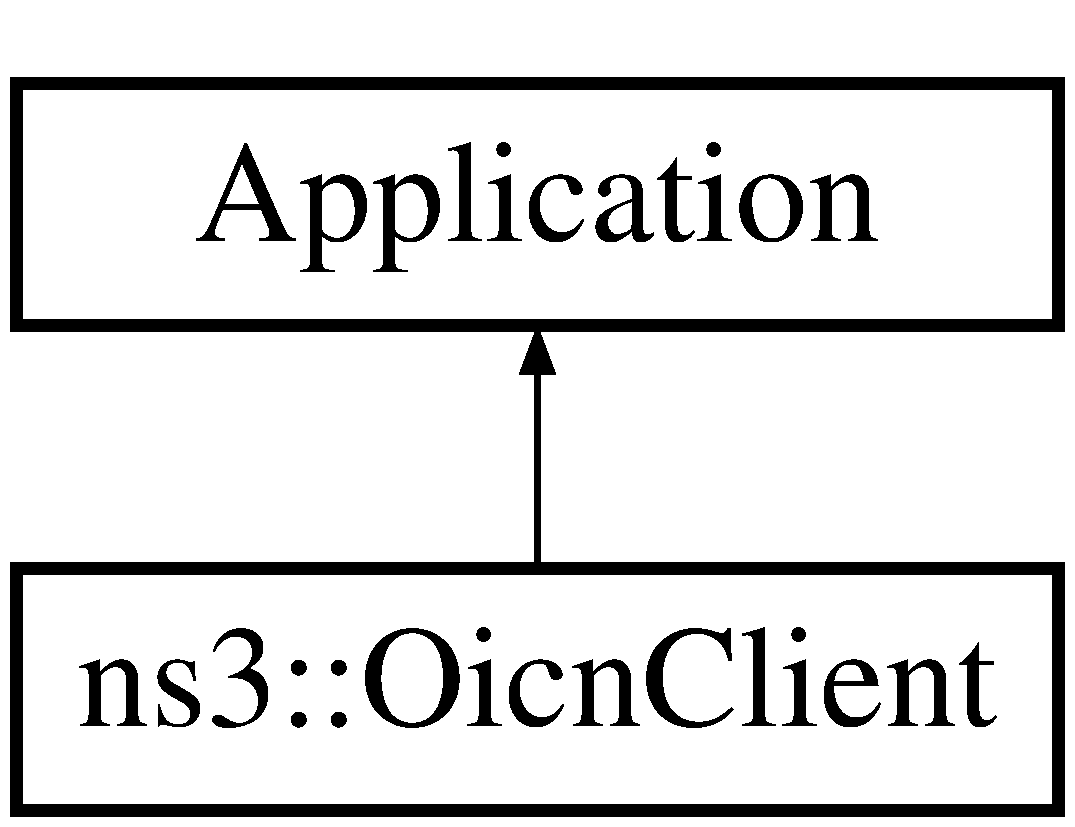
\includegraphics[height=2.000000cm]{classns3_1_1OicnClient}
\end{center}
\end{figure}
\subsection*{Public Member Functions}
\begin{DoxyCompactItemize}
\item 
\hyperlink{classns3_1_1OicnClient_a4cd258edda3827dcc5d59acee6464e28}{Oicn\-Client} ()
\item 
virtual \hyperlink{classns3_1_1OicnClient_afd1c9b766b88ee402b679e772dfcee03}{$\sim$\-Oicn\-Client} (void)
\item 
void \hyperlink{classns3_1_1OicnClient_a6877bfdc4f2ded46fdd439fef46451b6}{Set\-Content\-Index} (std\-::vector$<$ int $>$ index)
\begin{DoxyCompactList}\small\item\em Set the content index. Here name are constructed based upon index. \end{DoxyCompactList}\item 
Ptr$<$ Packet $>$ \hyperlink{classns3_1_1OicnClient_aee54bdaf8223b42a87ce534dfa01c9a3}{Construct\-Sublayer} (Ptr$<$ Packet $>$ packet, std\-::string name)
\begin{DoxyCompactList}\small\item\em construct the sublayer header \end{DoxyCompactList}\item 
Ptr$<$ Packet $>$ \hyperlink{classns3_1_1OicnClient_a3f5f0ae8d72fd152ef7e3258f5df7589}{Construct\-Dns\-Plus\-Header} (Ptr$<$ Packet $>$ packet)
\begin{DoxyCompactList}\small\item\em construct the D\-N\-S Plus header \end{DoxyCompactList}\item 
Ptr$<$ Packet $>$ \hyperlink{classns3_1_1OicnClient_a38a118f1203789a1062367c1cf71a7b6}{Construct\-Dns\-Plus\-Question} (Ptr$<$ Packet $>$ packet, std\-::string name)
\begin{DoxyCompactList}\small\item\em construct the D\-N\-S Plus Question Section \end{DoxyCompactList}\end{DoxyCompactItemize}
\subsection*{Static Public Member Functions}
\begin{DoxyCompactItemize}
\item 
static Type\-Id \hyperlink{classns3_1_1OicnClient_abd0403cc141fa16ba8351f6d30bab33d}{Get\-Type\-Id} (void)
\begin{DoxyCompactList}\small\item\em Get the type I\-D. \end{DoxyCompactList}\end{DoxyCompactItemize}
\subsection*{Protected Member Functions}
\begin{DoxyCompactItemize}
\item 
virtual void \hyperlink{classns3_1_1OicnClient_a31a8c315ffb1b3fd93b6fefd596921f1}{Do\-Dispose} (void)
\end{DoxyCompactItemize}
\subsection*{Private Member Functions}
\begin{DoxyCompactItemize}
\item 
void \hyperlink{classns3_1_1OicnClient_ac8a14bcce5fe31183ef90953041ab085}{Handle\-Read\-Icn\-Manager} (Ptr$<$ Socket $>$ socket)
\begin{DoxyCompactList}\small\item\em Handle a packet reception from I\-C\-N Manager port (36). This function is called by lower layers. \end{DoxyCompactList}\item 
void \hyperlink{classns3_1_1OicnClient_a5ec54db1f765e9694893eb16ea3bc1fd}{Handle\-Read\-Source} (Ptr$<$ Socket $>$ socket)
\begin{DoxyCompactList}\small\item\em Handle a packet reception from Source port (I\-C\-N Router or Server) (89). This function is called by lower layers. \end{DoxyCompactList}\item 
virtual void \hyperlink{classns3_1_1OicnClient_aef6c598503b815369cb5aca8c258d1b5}{Start\-Application} (void)
\item 
virtual void \hyperlink{classns3_1_1OicnClient_ad25f24d5c9067270e34762850d820959}{Stop\-Application} (void)
\item 
void \hyperlink{classns3_1_1OicnClient_afbc13131125b275ae6075a76bef32e45}{Schedule\-Transmit} (Time dt)
\begin{DoxyCompactList}\small\item\em Schedule the next packet transmission. \end{DoxyCompactList}\item 
void \hyperlink{classns3_1_1OicnClient_aa6912792d6fa9c629fc2d01607476537}{Send} (void)
\begin{DoxyCompactList}\small\item\em Send a packet to I\-C\-N Manager. \end{DoxyCompactList}\end{DoxyCompactItemize}
\subsection*{Private Attributes}
\begin{DoxyCompactItemize}
\item 
std\-::vector$<$ int $>$ \hyperlink{classns3_1_1OicnClient_aee7af038133594a358a77ea3ccece6d3}{m\-\_\-index}
\begin{DoxyCompactList}\small\item\em index of the content name, name of content are formed based on index \end{DoxyCompactList}\item 
uint32\-\_\-t \hyperlink{classns3_1_1OicnClient_a327312bc75b569a1982003fd61e3e45e}{m\-\_\-i}
\begin{DoxyCompactList}\small\item\em index of vector m\-\_\-index \end{DoxyCompactList}\item 
uint32\-\_\-t \hyperlink{classns3_1_1OicnClient_a5a15019661aa3b479f872b42c601cf36}{m\-\_\-sent}
\begin{DoxyCompactList}\small\item\em counter for sent packets \end{DoxyCompactList}\item 
uint32\-\_\-t \hyperlink{classns3_1_1OicnClient_af43386351e66788b1a53aa51b8a3d481}{m\-\_\-count}
\begin{DoxyCompactList}\small\item\em the maximum number of packets the application will send \end{DoxyCompactList}\item 
uint16\-\_\-t \hyperlink{classns3_1_1OicnClient_a96e719be70f2eb12ff391caf0a41367d}{m\-\_\-port\-Fixed}
\begin{DoxyCompactList}\small\item\em client port is attached with port no 26, it will listen to this port from O\-I\-C\-N Source(\-I\-C\-N router or server) \end{DoxyCompactList}\item 
Ptr$<$ Socket $>$ \hyperlink{classns3_1_1OicnClient_a6f062f8c4a35ad072f301141d986ba77}{m\-\_\-socket\-Icn\-Manager}
\begin{DoxyCompactList}\small\item\em socket associated with I\-C\-N Manager \end{DoxyCompactList}\item 
Ptr$<$ Socket $>$ \hyperlink{classns3_1_1OicnClient_a7903a89bbce331174829f0f83b932ca0}{m\-\_\-socket\-Source}
\begin{DoxyCompactList}\small\item\em socket associated with Source \end{DoxyCompactList}\item 
Event\-Id \hyperlink{classns3_1_1OicnClient_ad4f77ec10de5d2aad0c3b42f56c22c8c}{m\-\_\-send\-Event}
\begin{DoxyCompactList}\small\item\em event to send the next packet \end{DoxyCompactList}\item 
Time \hyperlink{classns3_1_1OicnClient_a4b3472531c624271e4fa7a2deb1d524c}{m\-\_\-interval}
\begin{DoxyCompactList}\small\item\em packet inter-\/send time \end{DoxyCompactList}\item 
Address \hyperlink{classns3_1_1OicnClient_a52010a30a1032d875127a331b734f107}{m\-\_\-icn\-Manager\-Address}
\begin{DoxyCompactList}\small\item\em I\-C\-N Manager Address. \end{DoxyCompactList}\item 
uint16\-\_\-t \hyperlink{classns3_1_1OicnClient_abb0ac949b2aeea8fb892065a0372d0cc}{m\-\_\-icn\-Manager\-Port}
\begin{DoxyCompactList}\small\item\em I\-C\-N Manager port. \end{DoxyCompactList}\end{DoxyCompactItemize}


\subsection{Detailed Description}
O\-I\-C\-N client application requests for content name resolution to I\-C\-N Manager. I\-C\-N Manager in turn resolve the name request and direct source of content (I\-C\-N router or server) to send the content to client. 

\subsection{Constructor \& Destructor Documentation}
\hypertarget{classns3_1_1OicnClient_a4cd258edda3827dcc5d59acee6464e28}{\index{ns3\-::\-Oicn\-Client@{ns3\-::\-Oicn\-Client}!Oicn\-Client@{Oicn\-Client}}
\index{Oicn\-Client@{Oicn\-Client}!ns3::OicnClient@{ns3\-::\-Oicn\-Client}}
\subsubsection[{Oicn\-Client}]{\setlength{\rightskip}{0pt plus 5cm}ns3\-::\-Oicn\-Client\-::\-Oicn\-Client (
\begin{DoxyParamCaption}
{}
\end{DoxyParamCaption}
)}}\label{classns3_1_1OicnClient_a4cd258edda3827dcc5d59acee6464e28}
\hypertarget{classns3_1_1OicnClient_afd1c9b766b88ee402b679e772dfcee03}{\index{ns3\-::\-Oicn\-Client@{ns3\-::\-Oicn\-Client}!$\sim$\-Oicn\-Client@{$\sim$\-Oicn\-Client}}
\index{$\sim$\-Oicn\-Client@{$\sim$\-Oicn\-Client}!ns3::OicnClient@{ns3\-::\-Oicn\-Client}}
\subsubsection[{$\sim$\-Oicn\-Client}]{\setlength{\rightskip}{0pt plus 5cm}ns3\-::\-Oicn\-Client\-::$\sim$\-Oicn\-Client (
\begin{DoxyParamCaption}
\item[{void}]{}
\end{DoxyParamCaption}
)\hspace{0.3cm}{\ttfamily [virtual]}}}\label{classns3_1_1OicnClient_afd1c9b766b88ee402b679e772dfcee03}


\subsection{Member Function Documentation}
\hypertarget{classns3_1_1OicnClient_a3f5f0ae8d72fd152ef7e3258f5df7589}{\index{ns3\-::\-Oicn\-Client@{ns3\-::\-Oicn\-Client}!Construct\-Dns\-Plus\-Header@{Construct\-Dns\-Plus\-Header}}
\index{Construct\-Dns\-Plus\-Header@{Construct\-Dns\-Plus\-Header}!ns3::OicnClient@{ns3\-::\-Oicn\-Client}}
\subsubsection[{Construct\-Dns\-Plus\-Header}]{\setlength{\rightskip}{0pt plus 5cm}Ptr$<$ Packet $>$ ns3\-::\-Oicn\-Client\-::\-Construct\-Dns\-Plus\-Header (
\begin{DoxyParamCaption}
\item[{Ptr$<$ Packet $>$}]{packet}
\end{DoxyParamCaption}
)}}\label{classns3_1_1OicnClient_a3f5f0ae8d72fd152ef7e3258f5df7589}


construct the D\-N\-S Plus header 


\begin{DoxyParams}{Parameters}
{\em packet} & packet being constructed by application layer \\
\hline
\end{DoxyParams}
\begin{DoxyReturn}{Returns}
packet constructed after adding D\-N\-S Plus header 
\end{DoxyReturn}
\hypertarget{classns3_1_1OicnClient_a38a118f1203789a1062367c1cf71a7b6}{\index{ns3\-::\-Oicn\-Client@{ns3\-::\-Oicn\-Client}!Construct\-Dns\-Plus\-Question@{Construct\-Dns\-Plus\-Question}}
\index{Construct\-Dns\-Plus\-Question@{Construct\-Dns\-Plus\-Question}!ns3::OicnClient@{ns3\-::\-Oicn\-Client}}
\subsubsection[{Construct\-Dns\-Plus\-Question}]{\setlength{\rightskip}{0pt plus 5cm}Ptr$<$ Packet $>$ ns3\-::\-Oicn\-Client\-::\-Construct\-Dns\-Plus\-Question (
\begin{DoxyParamCaption}
\item[{Ptr$<$ Packet $>$}]{packet, }
\item[{std\-::string}]{name}
\end{DoxyParamCaption}
)}}\label{classns3_1_1OicnClient_a38a118f1203789a1062367c1cf71a7b6}


construct the D\-N\-S Plus Question Section 


\begin{DoxyParams}{Parameters}
{\em packet} & packet being constructed by application layer \\
\hline
{\em name} & name of the content \\
\hline
\end{DoxyParams}
\begin{DoxyReturn}{Returns}
packet constructed after adding D\-N\-S Plus Question Section 
\end{DoxyReturn}
\hypertarget{classns3_1_1OicnClient_aee54bdaf8223b42a87ce534dfa01c9a3}{\index{ns3\-::\-Oicn\-Client@{ns3\-::\-Oicn\-Client}!Construct\-Sublayer@{Construct\-Sublayer}}
\index{Construct\-Sublayer@{Construct\-Sublayer}!ns3::OicnClient@{ns3\-::\-Oicn\-Client}}
\subsubsection[{Construct\-Sublayer}]{\setlength{\rightskip}{0pt plus 5cm}Ptr$<$ Packet $>$ ns3\-::\-Oicn\-Client\-::\-Construct\-Sublayer (
\begin{DoxyParamCaption}
\item[{Ptr$<$ Packet $>$}]{packet, }
\item[{std\-::string}]{name}
\end{DoxyParamCaption}
)}}\label{classns3_1_1OicnClient_aee54bdaf8223b42a87ce534dfa01c9a3}


construct the sublayer header 


\begin{DoxyParams}{Parameters}
{\em packet} & packet constructed by application layer \\
\hline
{\em name} & name of the content \\
\hline
\end{DoxyParams}
\begin{DoxyReturn}{Returns}
packet constructed after adding sublayer 
\end{DoxyReturn}
\hypertarget{classns3_1_1OicnClient_a31a8c315ffb1b3fd93b6fefd596921f1}{\index{ns3\-::\-Oicn\-Client@{ns3\-::\-Oicn\-Client}!Do\-Dispose@{Do\-Dispose}}
\index{Do\-Dispose@{Do\-Dispose}!ns3::OicnClient@{ns3\-::\-Oicn\-Client}}
\subsubsection[{Do\-Dispose}]{\setlength{\rightskip}{0pt plus 5cm}void ns3\-::\-Oicn\-Client\-::\-Do\-Dispose (
\begin{DoxyParamCaption}
\item[{void}]{}
\end{DoxyParamCaption}
)\hspace{0.3cm}{\ttfamily [protected]}, {\ttfamily [virtual]}}}\label{classns3_1_1OicnClient_a31a8c315ffb1b3fd93b6fefd596921f1}
\hypertarget{classns3_1_1OicnClient_abd0403cc141fa16ba8351f6d30bab33d}{\index{ns3\-::\-Oicn\-Client@{ns3\-::\-Oicn\-Client}!Get\-Type\-Id@{Get\-Type\-Id}}
\index{Get\-Type\-Id@{Get\-Type\-Id}!ns3::OicnClient@{ns3\-::\-Oicn\-Client}}
\subsubsection[{Get\-Type\-Id}]{\setlength{\rightskip}{0pt plus 5cm}Type\-Id ns3\-::\-Oicn\-Client\-::\-Get\-Type\-Id (
\begin{DoxyParamCaption}
\item[{void}]{}
\end{DoxyParamCaption}
)\hspace{0.3cm}{\ttfamily [static]}}}\label{classns3_1_1OicnClient_abd0403cc141fa16ba8351f6d30bab33d}


Get the type I\-D. 

\begin{DoxyReturn}{Returns}
the object Type\-Id 
\end{DoxyReturn}
\hypertarget{classns3_1_1OicnClient_ac8a14bcce5fe31183ef90953041ab085}{\index{ns3\-::\-Oicn\-Client@{ns3\-::\-Oicn\-Client}!Handle\-Read\-Icn\-Manager@{Handle\-Read\-Icn\-Manager}}
\index{Handle\-Read\-Icn\-Manager@{Handle\-Read\-Icn\-Manager}!ns3::OicnClient@{ns3\-::\-Oicn\-Client}}
\subsubsection[{Handle\-Read\-Icn\-Manager}]{\setlength{\rightskip}{0pt plus 5cm}void ns3\-::\-Oicn\-Client\-::\-Handle\-Read\-Icn\-Manager (
\begin{DoxyParamCaption}
\item[{Ptr$<$ Socket $>$}]{socket}
\end{DoxyParamCaption}
)\hspace{0.3cm}{\ttfamily [private]}}}\label{classns3_1_1OicnClient_ac8a14bcce5fe31183ef90953041ab085}


Handle a packet reception from I\-C\-N Manager port (36). This function is called by lower layers. 


\begin{DoxyParams}{Parameters}
{\em socket} & the socket the packet was received to. \\
\hline
\end{DoxyParams}
\hypertarget{classns3_1_1OicnClient_a5ec54db1f765e9694893eb16ea3bc1fd}{\index{ns3\-::\-Oicn\-Client@{ns3\-::\-Oicn\-Client}!Handle\-Read\-Source@{Handle\-Read\-Source}}
\index{Handle\-Read\-Source@{Handle\-Read\-Source}!ns3::OicnClient@{ns3\-::\-Oicn\-Client}}
\subsubsection[{Handle\-Read\-Source}]{\setlength{\rightskip}{0pt plus 5cm}void ns3\-::\-Oicn\-Client\-::\-Handle\-Read\-Source (
\begin{DoxyParamCaption}
\item[{Ptr$<$ Socket $>$}]{socket}
\end{DoxyParamCaption}
)\hspace{0.3cm}{\ttfamily [private]}}}\label{classns3_1_1OicnClient_a5ec54db1f765e9694893eb16ea3bc1fd}


Handle a packet reception from Source port (I\-C\-N Router or Server) (89). This function is called by lower layers. 


\begin{DoxyParams}{Parameters}
{\em socket} & the socket the packet was received to. \\
\hline
\end{DoxyParams}
\hypertarget{classns3_1_1OicnClient_afbc13131125b275ae6075a76bef32e45}{\index{ns3\-::\-Oicn\-Client@{ns3\-::\-Oicn\-Client}!Schedule\-Transmit@{Schedule\-Transmit}}
\index{Schedule\-Transmit@{Schedule\-Transmit}!ns3::OicnClient@{ns3\-::\-Oicn\-Client}}
\subsubsection[{Schedule\-Transmit}]{\setlength{\rightskip}{0pt plus 5cm}void ns3\-::\-Oicn\-Client\-::\-Schedule\-Transmit (
\begin{DoxyParamCaption}
\item[{Time}]{dt}
\end{DoxyParamCaption}
)\hspace{0.3cm}{\ttfamily [private]}}}\label{classns3_1_1OicnClient_afbc13131125b275ae6075a76bef32e45}


Schedule the next packet transmission. 


\begin{DoxyParams}{Parameters}
{\em dt} & time interval between packets. \\
\hline
\end{DoxyParams}
\hypertarget{classns3_1_1OicnClient_aa6912792d6fa9c629fc2d01607476537}{\index{ns3\-::\-Oicn\-Client@{ns3\-::\-Oicn\-Client}!Send@{Send}}
\index{Send@{Send}!ns3::OicnClient@{ns3\-::\-Oicn\-Client}}
\subsubsection[{Send}]{\setlength{\rightskip}{0pt plus 5cm}void ns3\-::\-Oicn\-Client\-::\-Send (
\begin{DoxyParamCaption}
\item[{void}]{}
\end{DoxyParamCaption}
)\hspace{0.3cm}{\ttfamily [private]}}}\label{classns3_1_1OicnClient_aa6912792d6fa9c629fc2d01607476537}


Send a packet to I\-C\-N Manager. 

\hypertarget{classns3_1_1OicnClient_a6877bfdc4f2ded46fdd439fef46451b6}{\index{ns3\-::\-Oicn\-Client@{ns3\-::\-Oicn\-Client}!Set\-Content\-Index@{Set\-Content\-Index}}
\index{Set\-Content\-Index@{Set\-Content\-Index}!ns3::OicnClient@{ns3\-::\-Oicn\-Client}}
\subsubsection[{Set\-Content\-Index}]{\setlength{\rightskip}{0pt plus 5cm}void ns3\-::\-Oicn\-Client\-::\-Set\-Content\-Index (
\begin{DoxyParamCaption}
\item[{std\-::vector$<$ int $>$}]{index}
\end{DoxyParamCaption}
)}}\label{classns3_1_1OicnClient_a6877bfdc4f2ded46fdd439fef46451b6}


Set the content index. Here name are constructed based upon index. 


\begin{DoxyParams}{Parameters}
{\em index} & value of the index \\
\hline
\end{DoxyParams}
\hypertarget{classns3_1_1OicnClient_aef6c598503b815369cb5aca8c258d1b5}{\index{ns3\-::\-Oicn\-Client@{ns3\-::\-Oicn\-Client}!Start\-Application@{Start\-Application}}
\index{Start\-Application@{Start\-Application}!ns3::OicnClient@{ns3\-::\-Oicn\-Client}}
\subsubsection[{Start\-Application}]{\setlength{\rightskip}{0pt plus 5cm}void ns3\-::\-Oicn\-Client\-::\-Start\-Application (
\begin{DoxyParamCaption}
\item[{void}]{}
\end{DoxyParamCaption}
)\hspace{0.3cm}{\ttfamily [private]}, {\ttfamily [virtual]}}}\label{classns3_1_1OicnClient_aef6c598503b815369cb5aca8c258d1b5}
\hypertarget{classns3_1_1OicnClient_ad25f24d5c9067270e34762850d820959}{\index{ns3\-::\-Oicn\-Client@{ns3\-::\-Oicn\-Client}!Stop\-Application@{Stop\-Application}}
\index{Stop\-Application@{Stop\-Application}!ns3::OicnClient@{ns3\-::\-Oicn\-Client}}
\subsubsection[{Stop\-Application}]{\setlength{\rightskip}{0pt plus 5cm}void ns3\-::\-Oicn\-Client\-::\-Stop\-Application (
\begin{DoxyParamCaption}
\item[{void}]{}
\end{DoxyParamCaption}
)\hspace{0.3cm}{\ttfamily [private]}, {\ttfamily [virtual]}}}\label{classns3_1_1OicnClient_ad25f24d5c9067270e34762850d820959}


\subsection{Member Data Documentation}
\hypertarget{classns3_1_1OicnClient_af43386351e66788b1a53aa51b8a3d481}{\index{ns3\-::\-Oicn\-Client@{ns3\-::\-Oicn\-Client}!m\-\_\-count@{m\-\_\-count}}
\index{m\-\_\-count@{m\-\_\-count}!ns3::OicnClient@{ns3\-::\-Oicn\-Client}}
\subsubsection[{m\-\_\-count}]{\setlength{\rightskip}{0pt plus 5cm}uint32\-\_\-t ns3\-::\-Oicn\-Client\-::m\-\_\-count\hspace{0.3cm}{\ttfamily [private]}}}\label{classns3_1_1OicnClient_af43386351e66788b1a53aa51b8a3d481}


the maximum number of packets the application will send 

\hypertarget{classns3_1_1OicnClient_a327312bc75b569a1982003fd61e3e45e}{\index{ns3\-::\-Oicn\-Client@{ns3\-::\-Oicn\-Client}!m\-\_\-i@{m\-\_\-i}}
\index{m\-\_\-i@{m\-\_\-i}!ns3::OicnClient@{ns3\-::\-Oicn\-Client}}
\subsubsection[{m\-\_\-i}]{\setlength{\rightskip}{0pt plus 5cm}uint32\-\_\-t ns3\-::\-Oicn\-Client\-::m\-\_\-i\hspace{0.3cm}{\ttfamily [private]}}}\label{classns3_1_1OicnClient_a327312bc75b569a1982003fd61e3e45e}


index of vector m\-\_\-index 

\hypertarget{classns3_1_1OicnClient_a52010a30a1032d875127a331b734f107}{\index{ns3\-::\-Oicn\-Client@{ns3\-::\-Oicn\-Client}!m\-\_\-icn\-Manager\-Address@{m\-\_\-icn\-Manager\-Address}}
\index{m\-\_\-icn\-Manager\-Address@{m\-\_\-icn\-Manager\-Address}!ns3::OicnClient@{ns3\-::\-Oicn\-Client}}
\subsubsection[{m\-\_\-icn\-Manager\-Address}]{\setlength{\rightskip}{0pt plus 5cm}Address ns3\-::\-Oicn\-Client\-::m\-\_\-icn\-Manager\-Address\hspace{0.3cm}{\ttfamily [private]}}}\label{classns3_1_1OicnClient_a52010a30a1032d875127a331b734f107}


I\-C\-N Manager Address. 

\hypertarget{classns3_1_1OicnClient_abb0ac949b2aeea8fb892065a0372d0cc}{\index{ns3\-::\-Oicn\-Client@{ns3\-::\-Oicn\-Client}!m\-\_\-icn\-Manager\-Port@{m\-\_\-icn\-Manager\-Port}}
\index{m\-\_\-icn\-Manager\-Port@{m\-\_\-icn\-Manager\-Port}!ns3::OicnClient@{ns3\-::\-Oicn\-Client}}
\subsubsection[{m\-\_\-icn\-Manager\-Port}]{\setlength{\rightskip}{0pt plus 5cm}uint16\-\_\-t ns3\-::\-Oicn\-Client\-::m\-\_\-icn\-Manager\-Port\hspace{0.3cm}{\ttfamily [private]}}}\label{classns3_1_1OicnClient_abb0ac949b2aeea8fb892065a0372d0cc}


I\-C\-N Manager port. 

\hypertarget{classns3_1_1OicnClient_aee7af038133594a358a77ea3ccece6d3}{\index{ns3\-::\-Oicn\-Client@{ns3\-::\-Oicn\-Client}!m\-\_\-index@{m\-\_\-index}}
\index{m\-\_\-index@{m\-\_\-index}!ns3::OicnClient@{ns3\-::\-Oicn\-Client}}
\subsubsection[{m\-\_\-index}]{\setlength{\rightskip}{0pt plus 5cm}std\-::vector$<$int$>$ ns3\-::\-Oicn\-Client\-::m\-\_\-index\hspace{0.3cm}{\ttfamily [private]}}}\label{classns3_1_1OicnClient_aee7af038133594a358a77ea3ccece6d3}


index of the content name, name of content are formed based on index 

\hypertarget{classns3_1_1OicnClient_a4b3472531c624271e4fa7a2deb1d524c}{\index{ns3\-::\-Oicn\-Client@{ns3\-::\-Oicn\-Client}!m\-\_\-interval@{m\-\_\-interval}}
\index{m\-\_\-interval@{m\-\_\-interval}!ns3::OicnClient@{ns3\-::\-Oicn\-Client}}
\subsubsection[{m\-\_\-interval}]{\setlength{\rightskip}{0pt plus 5cm}Time ns3\-::\-Oicn\-Client\-::m\-\_\-interval\hspace{0.3cm}{\ttfamily [private]}}}\label{classns3_1_1OicnClient_a4b3472531c624271e4fa7a2deb1d524c}


packet inter-\/send time 

\hypertarget{classns3_1_1OicnClient_a96e719be70f2eb12ff391caf0a41367d}{\index{ns3\-::\-Oicn\-Client@{ns3\-::\-Oicn\-Client}!m\-\_\-port\-Fixed@{m\-\_\-port\-Fixed}}
\index{m\-\_\-port\-Fixed@{m\-\_\-port\-Fixed}!ns3::OicnClient@{ns3\-::\-Oicn\-Client}}
\subsubsection[{m\-\_\-port\-Fixed}]{\setlength{\rightskip}{0pt plus 5cm}uint16\-\_\-t ns3\-::\-Oicn\-Client\-::m\-\_\-port\-Fixed\hspace{0.3cm}{\ttfamily [private]}}}\label{classns3_1_1OicnClient_a96e719be70f2eb12ff391caf0a41367d}


client port is attached with port no 26, it will listen to this port from O\-I\-C\-N Source(\-I\-C\-N router or server) 

\hypertarget{classns3_1_1OicnClient_ad4f77ec10de5d2aad0c3b42f56c22c8c}{\index{ns3\-::\-Oicn\-Client@{ns3\-::\-Oicn\-Client}!m\-\_\-send\-Event@{m\-\_\-send\-Event}}
\index{m\-\_\-send\-Event@{m\-\_\-send\-Event}!ns3::OicnClient@{ns3\-::\-Oicn\-Client}}
\subsubsection[{m\-\_\-send\-Event}]{\setlength{\rightskip}{0pt plus 5cm}Event\-Id ns3\-::\-Oicn\-Client\-::m\-\_\-send\-Event\hspace{0.3cm}{\ttfamily [private]}}}\label{classns3_1_1OicnClient_ad4f77ec10de5d2aad0c3b42f56c22c8c}


event to send the next packet 

\hypertarget{classns3_1_1OicnClient_a5a15019661aa3b479f872b42c601cf36}{\index{ns3\-::\-Oicn\-Client@{ns3\-::\-Oicn\-Client}!m\-\_\-sent@{m\-\_\-sent}}
\index{m\-\_\-sent@{m\-\_\-sent}!ns3::OicnClient@{ns3\-::\-Oicn\-Client}}
\subsubsection[{m\-\_\-sent}]{\setlength{\rightskip}{0pt plus 5cm}uint32\-\_\-t ns3\-::\-Oicn\-Client\-::m\-\_\-sent\hspace{0.3cm}{\ttfamily [private]}}}\label{classns3_1_1OicnClient_a5a15019661aa3b479f872b42c601cf36}


counter for sent packets 

\hypertarget{classns3_1_1OicnClient_a6f062f8c4a35ad072f301141d986ba77}{\index{ns3\-::\-Oicn\-Client@{ns3\-::\-Oicn\-Client}!m\-\_\-socket\-Icn\-Manager@{m\-\_\-socket\-Icn\-Manager}}
\index{m\-\_\-socket\-Icn\-Manager@{m\-\_\-socket\-Icn\-Manager}!ns3::OicnClient@{ns3\-::\-Oicn\-Client}}
\subsubsection[{m\-\_\-socket\-Icn\-Manager}]{\setlength{\rightskip}{0pt plus 5cm}Ptr$<$Socket$>$ ns3\-::\-Oicn\-Client\-::m\-\_\-socket\-Icn\-Manager\hspace{0.3cm}{\ttfamily [private]}}}\label{classns3_1_1OicnClient_a6f062f8c4a35ad072f301141d986ba77}


socket associated with I\-C\-N Manager 

\hypertarget{classns3_1_1OicnClient_a7903a89bbce331174829f0f83b932ca0}{\index{ns3\-::\-Oicn\-Client@{ns3\-::\-Oicn\-Client}!m\-\_\-socket\-Source@{m\-\_\-socket\-Source}}
\index{m\-\_\-socket\-Source@{m\-\_\-socket\-Source}!ns3::OicnClient@{ns3\-::\-Oicn\-Client}}
\subsubsection[{m\-\_\-socket\-Source}]{\setlength{\rightskip}{0pt plus 5cm}Ptr$<$Socket$>$ ns3\-::\-Oicn\-Client\-::m\-\_\-socket\-Source\hspace{0.3cm}{\ttfamily [private]}}}\label{classns3_1_1OicnClient_a7903a89bbce331174829f0f83b932ca0}


socket associated with Source 



The documentation for this class was generated from the following files\-:\begin{DoxyCompactItemize}
\item 
model/\hyperlink{oicn-client-application_8h}{oicn-\/client-\/application.\-h}\item 
model/\hyperlink{oicn-client-application_8cc}{oicn-\/client-\/application.\-cc}\end{DoxyCompactItemize}

\hypertarget{classns3_1_1OicnClientHelpher}{\section{ns3\-:\-:Oicn\-Client\-Helpher Class Reference}
\label{classns3_1_1OicnClientHelpher}\index{ns3\-::\-Oicn\-Client\-Helpher@{ns3\-::\-Oicn\-Client\-Helpher}}
}


Create a O\-I\-C\-N Client application which send content name resolution request to I\-C\-N Manager. I\-C\-N Manager direct the content request to I\-C\-N source (O\-I\-C\-N server or I\-C\-N router) which reply to O\-I\-C\-N client with requested content.  




{\ttfamily \#include $<$oicn-\/application-\/helper.\-h$>$}

\subsection*{Public Member Functions}
\begin{DoxyCompactItemize}
\item 
\hyperlink{classns3_1_1OicnClientHelpher_a8619c2f71ef3fc04f2b348dffe1ba98f}{Oicn\-Client\-Helpher} (Ipv4\-Address ip, uint16\-\_\-t port)
\item 
\hyperlink{classns3_1_1OicnClientHelpher_a34e23eea59e35ca63a59a4afcabc52cf}{Oicn\-Client\-Helpher} (Address address, uint16\-\_\-t port)
\item 
\hyperlink{classns3_1_1OicnClientHelpher_a9cc046926b6ed35a81453acbbd3b96a6}{Oicn\-Client\-Helpher} ()
\item 
void \hyperlink{classns3_1_1OicnClientHelpher_a11a83c357296fef47c261de8e5773c8f}{Set\-Attribute} (std\-::string name, const Attribute\-Value \&value)
\item 
Application\-Container \hyperlink{classns3_1_1OicnClientHelpher_a9092f106877f63dc98d290c8e58062af}{Install} (Ptr$<$ Node $>$ node, std\-::vector$<$ int $>$ index) const 
\item 
Application\-Container \hyperlink{classns3_1_1OicnClientHelpher_a1e40ddee6d66de8f8aabc6099e8499ba}{Install} (Ptr$<$ Node $>$ node, std\-::pair$<$ int, int $>$ range) const 
\item 
Application\-Container \hyperlink{classns3_1_1OicnClientHelpher_a7f475089dfdd7c221dada95b84ace165}{Install} (Node\-Container c, std\-::vector$<$ int $>$ index) const 
\item 
Application\-Container \hyperlink{classns3_1_1OicnClientHelpher_a97dfea27ebd1fea82d7055fbcba83e20}{Install} (Node\-Container c, std\-::pair$<$ int, int $>$ range) const 
\end{DoxyCompactItemize}
\subsection*{Private Member Functions}
\begin{DoxyCompactItemize}
\item 
Application\-Container \hyperlink{classns3_1_1OicnClientHelpher_a9479132ca656221e74b6ea587180d063}{Install\-Priv} (Ptr$<$ Node $>$ node, std\-::vector$<$ int $>$ index) const 
\item 
Application\-Container \hyperlink{classns3_1_1OicnClientHelpher_a1d0e2b4999138dfabbcb02281c236592}{Install\-Priv} (Ptr$<$ Node $>$ node, std\-::pair$<$ int, int $>$ range) const 
\end{DoxyCompactItemize}
\subsection*{Private Attributes}
\begin{DoxyCompactItemize}
\item 
Object\-Factory \hyperlink{classns3_1_1OicnClientHelpher_aa58d9af446cdcba7fbaf4a0f579962fe}{m\-\_\-factory}
\begin{DoxyCompactList}\small\item\em Object factory. \end{DoxyCompactList}\end{DoxyCompactItemize}


\subsection{Detailed Description}
Create a O\-I\-C\-N Client application which send content name resolution request to I\-C\-N Manager. I\-C\-N Manager direct the content request to I\-C\-N source (O\-I\-C\-N server or I\-C\-N router) which reply to O\-I\-C\-N client with requested content. 

\subsection{Constructor \& Destructor Documentation}
\hypertarget{classns3_1_1OicnClientHelpher_a8619c2f71ef3fc04f2b348dffe1ba98f}{\index{ns3\-::\-Oicn\-Client\-Helpher@{ns3\-::\-Oicn\-Client\-Helpher}!Oicn\-Client\-Helpher@{Oicn\-Client\-Helpher}}
\index{Oicn\-Client\-Helpher@{Oicn\-Client\-Helpher}!ns3::OicnClientHelpher@{ns3\-::\-Oicn\-Client\-Helpher}}
\subsubsection[{Oicn\-Client\-Helpher}]{\setlength{\rightskip}{0pt plus 5cm}ns3\-::\-Oicn\-Client\-Helpher\-::\-Oicn\-Client\-Helpher (
\begin{DoxyParamCaption}
\item[{Ipv4\-Address}]{ip, }
\item[{uint16\-\_\-t}]{port}
\end{DoxyParamCaption}
)}}\label{classns3_1_1OicnClientHelpher_a8619c2f71ef3fc04f2b348dffe1ba98f}
Create \hyperlink{classns3_1_1OicnClientHelpher}{Oicn\-Client\-Helpher} configured with I\-C\-N Manager I\-P address and port number.


\begin{DoxyParams}{Parameters}
{\em ip} & the I\-Pv4 address of the I\-C\-N Manager \\
\hline
{\em port} & the port number of the I\-C\-N Manager \\
\hline
\end{DoxyParams}
\hypertarget{classns3_1_1OicnClientHelpher_a34e23eea59e35ca63a59a4afcabc52cf}{\index{ns3\-::\-Oicn\-Client\-Helpher@{ns3\-::\-Oicn\-Client\-Helpher}!Oicn\-Client\-Helpher@{Oicn\-Client\-Helpher}}
\index{Oicn\-Client\-Helpher@{Oicn\-Client\-Helpher}!ns3::OicnClientHelpher@{ns3\-::\-Oicn\-Client\-Helpher}}
\subsubsection[{Oicn\-Client\-Helpher}]{\setlength{\rightskip}{0pt plus 5cm}ns3\-::\-Oicn\-Client\-Helpher\-::\-Oicn\-Client\-Helpher (
\begin{DoxyParamCaption}
\item[{Address}]{address, }
\item[{uint16\-\_\-t}]{port}
\end{DoxyParamCaption}
)}}\label{classns3_1_1OicnClientHelpher_a34e23eea59e35ca63a59a4afcabc52cf}
Create \hyperlink{classns3_1_1OicnClientHelpher}{Oicn\-Client\-Helpher} configured with I\-C\-N Manager I\-P address and port number.


\begin{DoxyParams}{Parameters}
{\em address} & the I\-P address of the I\-C\-N Manager \\
\hline
{\em port} & the port number of the I\-C\-N Manager \\
\hline
\end{DoxyParams}
\hypertarget{classns3_1_1OicnClientHelpher_a9cc046926b6ed35a81453acbbd3b96a6}{\index{ns3\-::\-Oicn\-Client\-Helpher@{ns3\-::\-Oicn\-Client\-Helpher}!Oicn\-Client\-Helpher@{Oicn\-Client\-Helpher}}
\index{Oicn\-Client\-Helpher@{Oicn\-Client\-Helpher}!ns3::OicnClientHelpher@{ns3\-::\-Oicn\-Client\-Helpher}}
\subsubsection[{Oicn\-Client\-Helpher}]{\setlength{\rightskip}{0pt plus 5cm}ns3\-::\-Oicn\-Client\-Helpher\-::\-Oicn\-Client\-Helpher (
\begin{DoxyParamCaption}
{}
\end{DoxyParamCaption}
)}}\label{classns3_1_1OicnClientHelpher_a9cc046926b6ed35a81453acbbd3b96a6}
\hyperlink{classns3_1_1OicnClientHelpher}{Oicn\-Client\-Helpher} 

\subsection{Member Function Documentation}
\hypertarget{classns3_1_1OicnClientHelpher_a9092f106877f63dc98d290c8e58062af}{\index{ns3\-::\-Oicn\-Client\-Helpher@{ns3\-::\-Oicn\-Client\-Helpher}!Install@{Install}}
\index{Install@{Install}!ns3::OicnClientHelpher@{ns3\-::\-Oicn\-Client\-Helpher}}
\subsubsection[{Install}]{\setlength{\rightskip}{0pt plus 5cm}Application\-Container ns3\-::\-Oicn\-Client\-Helpher\-::\-Install (
\begin{DoxyParamCaption}
\item[{Ptr$<$ Node $>$}]{node, }
\item[{std\-::vector$<$ int $>$}]{index}
\end{DoxyParamCaption}
) const}}\label{classns3_1_1OicnClientHelpher_a9092f106877f63dc98d290c8e58062af}
Create an \hyperlink{classns3_1_1OicnClient}{Oicn\-Client} Application querying the content specified by indices on the specified Node.


\begin{DoxyParams}{Parameters}
{\em node} & the node on which to create the Application. The node is specified by a Ptr$<$\-Node$>$ \\
\hline
{\em index} & vector containing the indices of the content to be queried \\
\hline
\end{DoxyParams}
\begin{DoxyReturn}{Returns}
an Application\-Container holding the Application created 
\end{DoxyReturn}
\hypertarget{classns3_1_1OicnClientHelpher_a1e40ddee6d66de8f8aabc6099e8499ba}{\index{ns3\-::\-Oicn\-Client\-Helpher@{ns3\-::\-Oicn\-Client\-Helpher}!Install@{Install}}
\index{Install@{Install}!ns3::OicnClientHelpher@{ns3\-::\-Oicn\-Client\-Helpher}}
\subsubsection[{Install}]{\setlength{\rightskip}{0pt plus 5cm}Application\-Container ns3\-::\-Oicn\-Client\-Helpher\-::\-Install (
\begin{DoxyParamCaption}
\item[{Ptr$<$ Node $>$}]{node, }
\item[{std\-::pair$<$ int, int $>$}]{range}
\end{DoxyParamCaption}
) const}}\label{classns3_1_1OicnClientHelpher_a1e40ddee6d66de8f8aabc6099e8499ba}
Create an \hyperlink{classns3_1_1OicnClient}{Oicn\-Client} Application querying the content specified by indices on the specified Node.


\begin{DoxyParams}{Parameters}
{\em node} & the node on which to create the Application. The node is specified by a Ptr$<$\-Node$>$ \\
\hline
{\em range} & range of the indices of the content to be queried \\
\hline
\end{DoxyParams}
\begin{DoxyReturn}{Returns}
an Application\-Container holding the Application created 
\end{DoxyReturn}
\hypertarget{classns3_1_1OicnClientHelpher_a7f475089dfdd7c221dada95b84ace165}{\index{ns3\-::\-Oicn\-Client\-Helpher@{ns3\-::\-Oicn\-Client\-Helpher}!Install@{Install}}
\index{Install@{Install}!ns3::OicnClientHelpher@{ns3\-::\-Oicn\-Client\-Helpher}}
\subsubsection[{Install}]{\setlength{\rightskip}{0pt plus 5cm}Application\-Container ns3\-::\-Oicn\-Client\-Helpher\-::\-Install (
\begin{DoxyParamCaption}
\item[{Node\-Container}]{c, }
\item[{std\-::vector$<$ int $>$}]{index}
\end{DoxyParamCaption}
) const}}\label{classns3_1_1OicnClientHelpher_a7f475089dfdd7c221dada95b84ace165}
Create an \hyperlink{classns3_1_1OicnClient}{Oicn\-Client} Application querying the content specified by indices on the specified Node.


\begin{DoxyParams}{Parameters}
{\em c} & the nodes on which to create the Applications. The nodes are specified by a Node\-Container \\
\hline
{\em index} & vector containing the indices of the content to be queried \\
\hline
\end{DoxyParams}
\begin{DoxyReturn}{Returns}
an Application\-Container holding the Application created 
\end{DoxyReturn}
\hypertarget{classns3_1_1OicnClientHelpher_a97dfea27ebd1fea82d7055fbcba83e20}{\index{ns3\-::\-Oicn\-Client\-Helpher@{ns3\-::\-Oicn\-Client\-Helpher}!Install@{Install}}
\index{Install@{Install}!ns3::OicnClientHelpher@{ns3\-::\-Oicn\-Client\-Helpher}}
\subsubsection[{Install}]{\setlength{\rightskip}{0pt plus 5cm}Application\-Container ns3\-::\-Oicn\-Client\-Helpher\-::\-Install (
\begin{DoxyParamCaption}
\item[{Node\-Container}]{c, }
\item[{std\-::pair$<$ int, int $>$}]{range}
\end{DoxyParamCaption}
) const}}\label{classns3_1_1OicnClientHelpher_a97dfea27ebd1fea82d7055fbcba83e20}
Create an \hyperlink{classns3_1_1OicnClient}{Oicn\-Client} Application querying the content specified by indices on the specified Node.


\begin{DoxyParams}{Parameters}
{\em c} & the nodes on which to create the Applications. The nodes are specified by a Node\-Container. \\
\hline
{\em range} & range of the indices of the content to be queried \\
\hline
\end{DoxyParams}
\begin{DoxyReturn}{Returns}
an Application\-Container holding the Application created 
\end{DoxyReturn}
\hypertarget{classns3_1_1OicnClientHelpher_a9479132ca656221e74b6ea587180d063}{\index{ns3\-::\-Oicn\-Client\-Helpher@{ns3\-::\-Oicn\-Client\-Helpher}!Install\-Priv@{Install\-Priv}}
\index{Install\-Priv@{Install\-Priv}!ns3::OicnClientHelpher@{ns3\-::\-Oicn\-Client\-Helpher}}
\subsubsection[{Install\-Priv}]{\setlength{\rightskip}{0pt plus 5cm}Application\-Container ns3\-::\-Oicn\-Client\-Helpher\-::\-Install\-Priv (
\begin{DoxyParamCaption}
\item[{Ptr$<$ Node $>$}]{node, }
\item[{std\-::vector$<$ int $>$}]{index}
\end{DoxyParamCaption}
) const\hspace{0.3cm}{\ttfamily [private]}}}\label{classns3_1_1OicnClientHelpher_a9479132ca656221e74b6ea587180d063}
Install an O\-I\-C\-N Client on the node configured with all the attributes set with Set\-Attribute.


\begin{DoxyParams}{Parameters}
{\em node} & the node on which an O\-I\-C\-N\-Client will be installed \\
\hline
{\em index} & vector containing the indices of the content \\
\hline
\end{DoxyParams}
\begin{DoxyReturn}{Returns}
an Application\-Container holding the Application created 
\end{DoxyReturn}
\hypertarget{classns3_1_1OicnClientHelpher_a1d0e2b4999138dfabbcb02281c236592}{\index{ns3\-::\-Oicn\-Client\-Helpher@{ns3\-::\-Oicn\-Client\-Helpher}!Install\-Priv@{Install\-Priv}}
\index{Install\-Priv@{Install\-Priv}!ns3::OicnClientHelpher@{ns3\-::\-Oicn\-Client\-Helpher}}
\subsubsection[{Install\-Priv}]{\setlength{\rightskip}{0pt plus 5cm}Application\-Container ns3\-::\-Oicn\-Client\-Helpher\-::\-Install\-Priv (
\begin{DoxyParamCaption}
\item[{Ptr$<$ Node $>$}]{node, }
\item[{std\-::pair$<$ int, int $>$}]{range}
\end{DoxyParamCaption}
) const\hspace{0.3cm}{\ttfamily [private]}}}\label{classns3_1_1OicnClientHelpher_a1d0e2b4999138dfabbcb02281c236592}
Install an O\-I\-C\-N Client on the node configured with all the attributes set with Set\-Attribute.


\begin{DoxyParams}{Parameters}
{\em node} & the node on which an O\-I\-C\-N\-Client will be installed \\
\hline
{\em range} & range of the indices of the content to be queried \\
\hline
\end{DoxyParams}
\begin{DoxyReturn}{Returns}
an Application\-Container holding the Application created 
\end{DoxyReturn}
\hypertarget{classns3_1_1OicnClientHelpher_a11a83c357296fef47c261de8e5773c8f}{\index{ns3\-::\-Oicn\-Client\-Helpher@{ns3\-::\-Oicn\-Client\-Helpher}!Set\-Attribute@{Set\-Attribute}}
\index{Set\-Attribute@{Set\-Attribute}!ns3::OicnClientHelpher@{ns3\-::\-Oicn\-Client\-Helpher}}
\subsubsection[{Set\-Attribute}]{\setlength{\rightskip}{0pt plus 5cm}void ns3\-::\-Oicn\-Client\-Helpher\-::\-Set\-Attribute (
\begin{DoxyParamCaption}
\item[{std\-::string}]{name, }
\item[{const Attribute\-Value \&}]{value}
\end{DoxyParamCaption}
)}}\label{classns3_1_1OicnClientHelpher_a11a83c357296fef47c261de8e5773c8f}
Record an attribute to be set in each Application after it is is created.


\begin{DoxyParams}{Parameters}
{\em name} & the name of the attribute to set \\
\hline
{\em value} & the value of the attribute to set \\
\hline
\end{DoxyParams}


\subsection{Member Data Documentation}
\hypertarget{classns3_1_1OicnClientHelpher_aa58d9af446cdcba7fbaf4a0f579962fe}{\index{ns3\-::\-Oicn\-Client\-Helpher@{ns3\-::\-Oicn\-Client\-Helpher}!m\-\_\-factory@{m\-\_\-factory}}
\index{m\-\_\-factory@{m\-\_\-factory}!ns3::OicnClientHelpher@{ns3\-::\-Oicn\-Client\-Helpher}}
\subsubsection[{m\-\_\-factory}]{\setlength{\rightskip}{0pt plus 5cm}Object\-Factory ns3\-::\-Oicn\-Client\-Helpher\-::m\-\_\-factory\hspace{0.3cm}{\ttfamily [private]}}}\label{classns3_1_1OicnClientHelpher_aa58d9af446cdcba7fbaf4a0f579962fe}


Object factory. 



The documentation for this class was generated from the following files\-:\begin{DoxyCompactItemize}
\item 
helper/\hyperlink{oicn-application-helper_8h}{oicn-\/application-\/helper.\-h}\item 
helper/\hyperlink{oicn-application-helper_8cc}{oicn-\/application-\/helper.\-cc}\end{DoxyCompactItemize}

\hypertarget{classns3_1_1OicnHeader}{\section{ns3\-:\-:Oicn\-Header Class Reference}
\label{classns3_1_1OicnHeader}\index{ns3\-::\-Oicn\-Header@{ns3\-::\-Oicn\-Header}}
}


Class for Creating and Appending O-\/\-I\-C\-N Sublayer to a Packet.  




{\ttfamily \#include $<$oicn-\/header.\-h$>$}

Inheritance diagram for ns3\-:\-:Oicn\-Header\-:\begin{figure}[H]
\begin{center}
\leavevmode
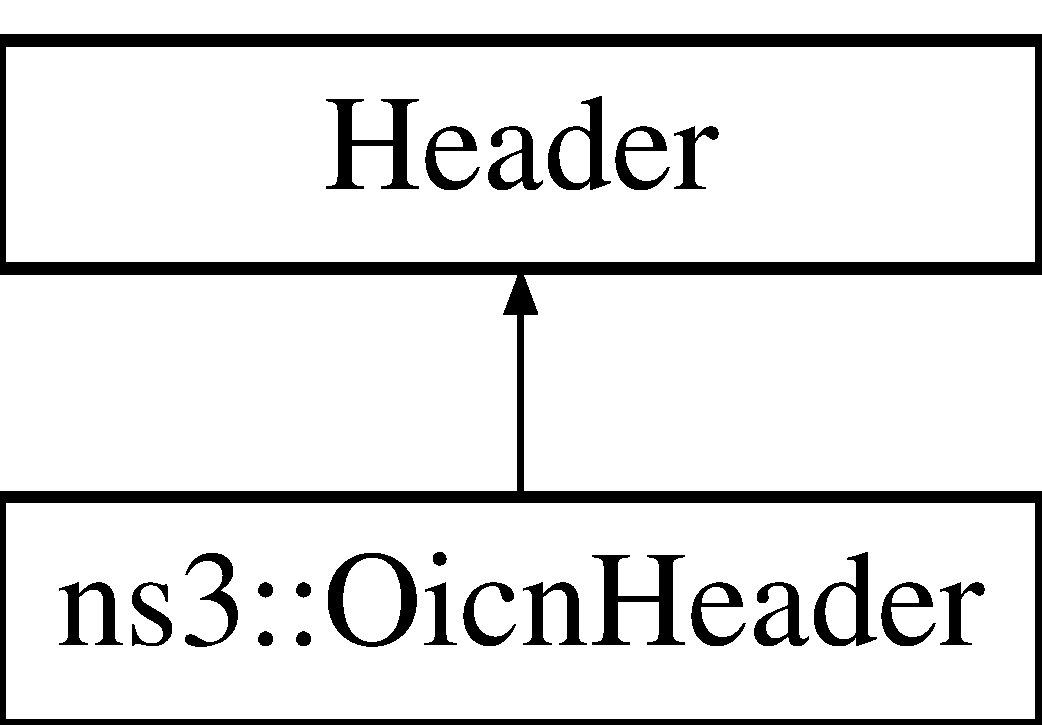
\includegraphics[height=2.000000cm]{classns3_1_1OicnHeader}
\end{center}
\end{figure}
\subsection*{Public Member Functions}
\begin{DoxyCompactItemize}
\item 
\hyperlink{classns3_1_1OicnHeader_a496135b4907b91cabe5387a4917994a5}{Oicn\-Header} ()
\item 
\hyperlink{classns3_1_1OicnHeader_af7ce0b989e6cd7123b984bcfb205150d}{$\sim$\-Oicn\-Header} ()
\item 
virtual Type\-Id \hyperlink{classns3_1_1OicnHeader_a39c2a2431d2aef132ac52e1d1ab1e892}{Get\-Instance\-Type\-Id} (void) const 
\item 
virtual uint32\-\_\-t \hyperlink{classns3_1_1OicnHeader_a4b0ba5fa4fe164e9e42a23a9a7b43268}{Get\-Serialized\-Size} (void) const 
\item 
virtual void \hyperlink{classns3_1_1OicnHeader_a427490fecb88ecfdb3576ab39ed31f5e}{Serialize} (Buffer\-::\-Iterator start) const 
\item 
virtual uint32\-\_\-t \hyperlink{classns3_1_1OicnHeader_af16eaf62f9048fe56e714f44459f754d}{Deserialize} (Buffer\-::\-Iterator start)
\item 
virtual void \hyperlink{classns3_1_1OicnHeader_ac5b6b41e69772b2c018adc0c313fc315}{Print} (std\-::ostream \&os) const 
\item 
void \hyperlink{classns3_1_1OicnHeader_afd6c18de6e052e61ed4de112c5724a18}{Set\-Name} (std\-::string name)
\item 
std\-::string \hyperlink{classns3_1_1OicnHeader_a00f48c0a31a66618f6c92431520801c3}{Get\-Name} (void)
\item 
void \hyperlink{classns3_1_1OicnHeader_ad49869449f12e894cc2dfb193d1a0181}{Set\-Request} (void)
\item 
void \hyperlink{classns3_1_1OicnHeader_a08a99a9ac99df2fca8af740137d47992}{Set\-Cachable} (void)
\item 
void \hyperlink{classns3_1_1OicnHeader_aa1e7e27b1b855587f0bf855c77b1ad64}{Set\-Non\-Cachable} (void)
\item 
uint32\-\_\-t \hyperlink{classns3_1_1OicnHeader_a9b5651fe0d172672e3e020c5df84a1c1}{Get\-First4\-Bytes} (void)
\end{DoxyCompactItemize}
\subsection*{Static Public Member Functions}
\begin{DoxyCompactItemize}
\item 
static Type\-Id \hyperlink{classns3_1_1OicnHeader_a275c1bad03b9f9ec4f11346a93061ac6}{Get\-Type\-Id} (void)
\end{DoxyCompactItemize}
\subsection*{Private Member Functions}
\begin{DoxyCompactItemize}
\item 
void \hyperlink{classns3_1_1OicnHeader_a6d775da4ae5ddd0b71f478422add3d68}{Set\-First4\-Bytes} (uint32\-\_\-t Header\-Length, bool reply, bool cachable)
\end{DoxyCompactItemize}
\subsection*{Private Attributes}
\begin{DoxyCompactItemize}
\item 
std\-::string \hyperlink{classns3_1_1OicnHeader_a4ec6866334efab8674e2b0d96837a4ae}{m\-\_\-name}
\item 
uint32\-\_\-t \hyperlink{classns3_1_1OicnHeader_a4992cefc6d31c27977363db61c068111}{header\-\_\-length}
\item 
uint32\-\_\-t \hyperlink{classns3_1_1OicnHeader_ac4f7599f027c10e4433efdcb8541ef38}{first4bytes}
\end{DoxyCompactItemize}
\subsection*{Static Private Attributes}
\begin{DoxyCompactItemize}
\item 
static const uint32\-\_\-t \hyperlink{classns3_1_1OicnHeader_af3b93655facbb38e13c98576c4454ec2}{cachable\-\_\-start} = 4026531840
\item 
static const uint32\-\_\-t \hyperlink{classns3_1_1OicnHeader_a822030e2b6549b78e31c440f4fe1f458}{non\-\_\-cachable\-\_\-start} = 2952790016
\item 
static const uint32\-\_\-t \hyperlink{classns3_1_1OicnHeader_a9fa69f9639455b3ed94cbb616e2809c0}{request\-\_\-start} = 805306368
\end{DoxyCompactItemize}


\subsection{Detailed Description}
Class for Creating and Appending O-\/\-I\-C\-N Sublayer to a Packet. 

This class has fields corresponding to those in a network U\-D\-P header (port numbers, payload size, checksum) as well as methods for serialization to and deserialization from a byte buffer. 

\subsection{Constructor \& Destructor Documentation}
\hypertarget{classns3_1_1OicnHeader_a496135b4907b91cabe5387a4917994a5}{\index{ns3\-::\-Oicn\-Header@{ns3\-::\-Oicn\-Header}!Oicn\-Header@{Oicn\-Header}}
\index{Oicn\-Header@{Oicn\-Header}!ns3::OicnHeader@{ns3\-::\-Oicn\-Header}}
\subsubsection[{Oicn\-Header}]{\setlength{\rightskip}{0pt plus 5cm}ns3\-::\-Oicn\-Header\-::\-Oicn\-Header (
\begin{DoxyParamCaption}
{}
\end{DoxyParamCaption}
)}}\label{classns3_1_1OicnHeader_a496135b4907b91cabe5387a4917994a5}
\hypertarget{classns3_1_1OicnHeader_af7ce0b989e6cd7123b984bcfb205150d}{\index{ns3\-::\-Oicn\-Header@{ns3\-::\-Oicn\-Header}!$\sim$\-Oicn\-Header@{$\sim$\-Oicn\-Header}}
\index{$\sim$\-Oicn\-Header@{$\sim$\-Oicn\-Header}!ns3::OicnHeader@{ns3\-::\-Oicn\-Header}}
\subsubsection[{$\sim$\-Oicn\-Header}]{\setlength{\rightskip}{0pt plus 5cm}ns3\-::\-Oicn\-Header\-::$\sim$\-Oicn\-Header (
\begin{DoxyParamCaption}
{}
\end{DoxyParamCaption}
)}}\label{classns3_1_1OicnHeader_af7ce0b989e6cd7123b984bcfb205150d}


\subsection{Member Function Documentation}
\hypertarget{classns3_1_1OicnHeader_af16eaf62f9048fe56e714f44459f754d}{\index{ns3\-::\-Oicn\-Header@{ns3\-::\-Oicn\-Header}!Deserialize@{Deserialize}}
\index{Deserialize@{Deserialize}!ns3::OicnHeader@{ns3\-::\-Oicn\-Header}}
\subsubsection[{Deserialize}]{\setlength{\rightskip}{0pt plus 5cm}uint32\-\_\-t ns3\-::\-Oicn\-Header\-::\-Deserialize (
\begin{DoxyParamCaption}
\item[{Buffer\-::\-Iterator}]{start}
\end{DoxyParamCaption}
)\hspace{0.3cm}{\ttfamily [virtual]}}}\label{classns3_1_1OicnHeader_af16eaf62f9048fe56e714f44459f754d}
\hypertarget{classns3_1_1OicnHeader_a9b5651fe0d172672e3e020c5df84a1c1}{\index{ns3\-::\-Oicn\-Header@{ns3\-::\-Oicn\-Header}!Get\-First4\-Bytes@{Get\-First4\-Bytes}}
\index{Get\-First4\-Bytes@{Get\-First4\-Bytes}!ns3::OicnHeader@{ns3\-::\-Oicn\-Header}}
\subsubsection[{Get\-First4\-Bytes}]{\setlength{\rightskip}{0pt plus 5cm}uint32\-\_\-t ns3\-::\-Oicn\-Header\-::\-Get\-First4\-Bytes (
\begin{DoxyParamCaption}
\item[{void}]{}
\end{DoxyParamCaption}
)}}\label{classns3_1_1OicnHeader_a9b5651fe0d172672e3e020c5df84a1c1}
\hypertarget{classns3_1_1OicnHeader_a39c2a2431d2aef132ac52e1d1ab1e892}{\index{ns3\-::\-Oicn\-Header@{ns3\-::\-Oicn\-Header}!Get\-Instance\-Type\-Id@{Get\-Instance\-Type\-Id}}
\index{Get\-Instance\-Type\-Id@{Get\-Instance\-Type\-Id}!ns3::OicnHeader@{ns3\-::\-Oicn\-Header}}
\subsubsection[{Get\-Instance\-Type\-Id}]{\setlength{\rightskip}{0pt plus 5cm}Type\-Id ns3\-::\-Oicn\-Header\-::\-Get\-Instance\-Type\-Id (
\begin{DoxyParamCaption}
\item[{void}]{}
\end{DoxyParamCaption}
) const\hspace{0.3cm}{\ttfamily [virtual]}}}\label{classns3_1_1OicnHeader_a39c2a2431d2aef132ac52e1d1ab1e892}
\hypertarget{classns3_1_1OicnHeader_a00f48c0a31a66618f6c92431520801c3}{\index{ns3\-::\-Oicn\-Header@{ns3\-::\-Oicn\-Header}!Get\-Name@{Get\-Name}}
\index{Get\-Name@{Get\-Name}!ns3::OicnHeader@{ns3\-::\-Oicn\-Header}}
\subsubsection[{Get\-Name}]{\setlength{\rightskip}{0pt plus 5cm}std\-::string ns3\-::\-Oicn\-Header\-::\-Get\-Name (
\begin{DoxyParamCaption}
\item[{void}]{}
\end{DoxyParamCaption}
)}}\label{classns3_1_1OicnHeader_a00f48c0a31a66618f6c92431520801c3}
\hypertarget{classns3_1_1OicnHeader_a4b0ba5fa4fe164e9e42a23a9a7b43268}{\index{ns3\-::\-Oicn\-Header@{ns3\-::\-Oicn\-Header}!Get\-Serialized\-Size@{Get\-Serialized\-Size}}
\index{Get\-Serialized\-Size@{Get\-Serialized\-Size}!ns3::OicnHeader@{ns3\-::\-Oicn\-Header}}
\subsubsection[{Get\-Serialized\-Size}]{\setlength{\rightskip}{0pt plus 5cm}uint32\-\_\-t ns3\-::\-Oicn\-Header\-::\-Get\-Serialized\-Size (
\begin{DoxyParamCaption}
\item[{void}]{}
\end{DoxyParamCaption}
) const\hspace{0.3cm}{\ttfamily [virtual]}}}\label{classns3_1_1OicnHeader_a4b0ba5fa4fe164e9e42a23a9a7b43268}
\hypertarget{classns3_1_1OicnHeader_a275c1bad03b9f9ec4f11346a93061ac6}{\index{ns3\-::\-Oicn\-Header@{ns3\-::\-Oicn\-Header}!Get\-Type\-Id@{Get\-Type\-Id}}
\index{Get\-Type\-Id@{Get\-Type\-Id}!ns3::OicnHeader@{ns3\-::\-Oicn\-Header}}
\subsubsection[{Get\-Type\-Id}]{\setlength{\rightskip}{0pt plus 5cm}Type\-Id ns3\-::\-Oicn\-Header\-::\-Get\-Type\-Id (
\begin{DoxyParamCaption}
\item[{void}]{}
\end{DoxyParamCaption}
)\hspace{0.3cm}{\ttfamily [static]}}}\label{classns3_1_1OicnHeader_a275c1bad03b9f9ec4f11346a93061ac6}
\hypertarget{classns3_1_1OicnHeader_ac5b6b41e69772b2c018adc0c313fc315}{\index{ns3\-::\-Oicn\-Header@{ns3\-::\-Oicn\-Header}!Print@{Print}}
\index{Print@{Print}!ns3::OicnHeader@{ns3\-::\-Oicn\-Header}}
\subsubsection[{Print}]{\setlength{\rightskip}{0pt plus 5cm}void ns3\-::\-Oicn\-Header\-::\-Print (
\begin{DoxyParamCaption}
\item[{std\-::ostream \&}]{os}
\end{DoxyParamCaption}
) const\hspace{0.3cm}{\ttfamily [virtual]}}}\label{classns3_1_1OicnHeader_ac5b6b41e69772b2c018adc0c313fc315}
\hypertarget{classns3_1_1OicnHeader_a427490fecb88ecfdb3576ab39ed31f5e}{\index{ns3\-::\-Oicn\-Header@{ns3\-::\-Oicn\-Header}!Serialize@{Serialize}}
\index{Serialize@{Serialize}!ns3::OicnHeader@{ns3\-::\-Oicn\-Header}}
\subsubsection[{Serialize}]{\setlength{\rightskip}{0pt plus 5cm}void ns3\-::\-Oicn\-Header\-::\-Serialize (
\begin{DoxyParamCaption}
\item[{Buffer\-::\-Iterator}]{start}
\end{DoxyParamCaption}
) const\hspace{0.3cm}{\ttfamily [virtual]}}}\label{classns3_1_1OicnHeader_a427490fecb88ecfdb3576ab39ed31f5e}
\hypertarget{classns3_1_1OicnHeader_a08a99a9ac99df2fca8af740137d47992}{\index{ns3\-::\-Oicn\-Header@{ns3\-::\-Oicn\-Header}!Set\-Cachable@{Set\-Cachable}}
\index{Set\-Cachable@{Set\-Cachable}!ns3::OicnHeader@{ns3\-::\-Oicn\-Header}}
\subsubsection[{Set\-Cachable}]{\setlength{\rightskip}{0pt plus 5cm}void ns3\-::\-Oicn\-Header\-::\-Set\-Cachable (
\begin{DoxyParamCaption}
\item[{void}]{}
\end{DoxyParamCaption}
)}}\label{classns3_1_1OicnHeader_a08a99a9ac99df2fca8af740137d47992}
\hypertarget{classns3_1_1OicnHeader_a6d775da4ae5ddd0b71f478422add3d68}{\index{ns3\-::\-Oicn\-Header@{ns3\-::\-Oicn\-Header}!Set\-First4\-Bytes@{Set\-First4\-Bytes}}
\index{Set\-First4\-Bytes@{Set\-First4\-Bytes}!ns3::OicnHeader@{ns3\-::\-Oicn\-Header}}
\subsubsection[{Set\-First4\-Bytes}]{\setlength{\rightskip}{0pt plus 5cm}void ns3\-::\-Oicn\-Header\-::\-Set\-First4\-Bytes (
\begin{DoxyParamCaption}
\item[{uint32\-\_\-t}]{Header\-Length, }
\item[{bool}]{reply, }
\item[{bool}]{cachable}
\end{DoxyParamCaption}
)\hspace{0.3cm}{\ttfamily [private]}}}\label{classns3_1_1OicnHeader_a6d775da4ae5ddd0b71f478422add3d68}
\hypertarget{classns3_1_1OicnHeader_afd6c18de6e052e61ed4de112c5724a18}{\index{ns3\-::\-Oicn\-Header@{ns3\-::\-Oicn\-Header}!Set\-Name@{Set\-Name}}
\index{Set\-Name@{Set\-Name}!ns3::OicnHeader@{ns3\-::\-Oicn\-Header}}
\subsubsection[{Set\-Name}]{\setlength{\rightskip}{0pt plus 5cm}void ns3\-::\-Oicn\-Header\-::\-Set\-Name (
\begin{DoxyParamCaption}
\item[{std\-::string}]{name}
\end{DoxyParamCaption}
)}}\label{classns3_1_1OicnHeader_afd6c18de6e052e61ed4de112c5724a18}
\hypertarget{classns3_1_1OicnHeader_aa1e7e27b1b855587f0bf855c77b1ad64}{\index{ns3\-::\-Oicn\-Header@{ns3\-::\-Oicn\-Header}!Set\-Non\-Cachable@{Set\-Non\-Cachable}}
\index{Set\-Non\-Cachable@{Set\-Non\-Cachable}!ns3::OicnHeader@{ns3\-::\-Oicn\-Header}}
\subsubsection[{Set\-Non\-Cachable}]{\setlength{\rightskip}{0pt plus 5cm}void ns3\-::\-Oicn\-Header\-::\-Set\-Non\-Cachable (
\begin{DoxyParamCaption}
\item[{void}]{}
\end{DoxyParamCaption}
)}}\label{classns3_1_1OicnHeader_aa1e7e27b1b855587f0bf855c77b1ad64}
\hypertarget{classns3_1_1OicnHeader_ad49869449f12e894cc2dfb193d1a0181}{\index{ns3\-::\-Oicn\-Header@{ns3\-::\-Oicn\-Header}!Set\-Request@{Set\-Request}}
\index{Set\-Request@{Set\-Request}!ns3::OicnHeader@{ns3\-::\-Oicn\-Header}}
\subsubsection[{Set\-Request}]{\setlength{\rightskip}{0pt plus 5cm}void ns3\-::\-Oicn\-Header\-::\-Set\-Request (
\begin{DoxyParamCaption}
\item[{void}]{}
\end{DoxyParamCaption}
)}}\label{classns3_1_1OicnHeader_ad49869449f12e894cc2dfb193d1a0181}


\subsection{Member Data Documentation}
\hypertarget{classns3_1_1OicnHeader_af3b93655facbb38e13c98576c4454ec2}{\index{ns3\-::\-Oicn\-Header@{ns3\-::\-Oicn\-Header}!cachable\-\_\-start@{cachable\-\_\-start}}
\index{cachable\-\_\-start@{cachable\-\_\-start}!ns3::OicnHeader@{ns3\-::\-Oicn\-Header}}
\subsubsection[{cachable\-\_\-start}]{\setlength{\rightskip}{0pt plus 5cm}const uint32\-\_\-t ns3\-::\-Oicn\-Header\-::cachable\-\_\-start = 4026531840\hspace{0.3cm}{\ttfamily [static]}, {\ttfamily [private]}}}\label{classns3_1_1OicnHeader_af3b93655facbb38e13c98576c4454ec2}
\hypertarget{classns3_1_1OicnHeader_ac4f7599f027c10e4433efdcb8541ef38}{\index{ns3\-::\-Oicn\-Header@{ns3\-::\-Oicn\-Header}!first4bytes@{first4bytes}}
\index{first4bytes@{first4bytes}!ns3::OicnHeader@{ns3\-::\-Oicn\-Header}}
\subsubsection[{first4bytes}]{\setlength{\rightskip}{0pt plus 5cm}uint32\-\_\-t ns3\-::\-Oicn\-Header\-::first4bytes\hspace{0.3cm}{\ttfamily [private]}}}\label{classns3_1_1OicnHeader_ac4f7599f027c10e4433efdcb8541ef38}
\hypertarget{classns3_1_1OicnHeader_a4992cefc6d31c27977363db61c068111}{\index{ns3\-::\-Oicn\-Header@{ns3\-::\-Oicn\-Header}!header\-\_\-length@{header\-\_\-length}}
\index{header\-\_\-length@{header\-\_\-length}!ns3::OicnHeader@{ns3\-::\-Oicn\-Header}}
\subsubsection[{header\-\_\-length}]{\setlength{\rightskip}{0pt plus 5cm}uint32\-\_\-t ns3\-::\-Oicn\-Header\-::header\-\_\-length\hspace{0.3cm}{\ttfamily [private]}}}\label{classns3_1_1OicnHeader_a4992cefc6d31c27977363db61c068111}
\hypertarget{classns3_1_1OicnHeader_a4ec6866334efab8674e2b0d96837a4ae}{\index{ns3\-::\-Oicn\-Header@{ns3\-::\-Oicn\-Header}!m\-\_\-name@{m\-\_\-name}}
\index{m\-\_\-name@{m\-\_\-name}!ns3::OicnHeader@{ns3\-::\-Oicn\-Header}}
\subsubsection[{m\-\_\-name}]{\setlength{\rightskip}{0pt plus 5cm}std\-::string ns3\-::\-Oicn\-Header\-::m\-\_\-name\hspace{0.3cm}{\ttfamily [private]}}}\label{classns3_1_1OicnHeader_a4ec6866334efab8674e2b0d96837a4ae}
\hypertarget{classns3_1_1OicnHeader_a822030e2b6549b78e31c440f4fe1f458}{\index{ns3\-::\-Oicn\-Header@{ns3\-::\-Oicn\-Header}!non\-\_\-cachable\-\_\-start@{non\-\_\-cachable\-\_\-start}}
\index{non\-\_\-cachable\-\_\-start@{non\-\_\-cachable\-\_\-start}!ns3::OicnHeader@{ns3\-::\-Oicn\-Header}}
\subsubsection[{non\-\_\-cachable\-\_\-start}]{\setlength{\rightskip}{0pt plus 5cm}const uint32\-\_\-t ns3\-::\-Oicn\-Header\-::non\-\_\-cachable\-\_\-start = 2952790016\hspace{0.3cm}{\ttfamily [static]}, {\ttfamily [private]}}}\label{classns3_1_1OicnHeader_a822030e2b6549b78e31c440f4fe1f458}
\hypertarget{classns3_1_1OicnHeader_a9fa69f9639455b3ed94cbb616e2809c0}{\index{ns3\-::\-Oicn\-Header@{ns3\-::\-Oicn\-Header}!request\-\_\-start@{request\-\_\-start}}
\index{request\-\_\-start@{request\-\_\-start}!ns3::OicnHeader@{ns3\-::\-Oicn\-Header}}
\subsubsection[{request\-\_\-start}]{\setlength{\rightskip}{0pt plus 5cm}const uint32\-\_\-t ns3\-::\-Oicn\-Header\-::request\-\_\-start = 805306368\hspace{0.3cm}{\ttfamily [static]}, {\ttfamily [private]}}}\label{classns3_1_1OicnHeader_a9fa69f9639455b3ed94cbb616e2809c0}


The documentation for this class was generated from the following files\-:\begin{DoxyCompactItemize}
\item 
model/\hyperlink{oicn-header_8h}{oicn-\/header.\-h}\item 
model/\hyperlink{oicn-header_8cc}{oicn-\/header.\-cc}\end{DoxyCompactItemize}

\hypertarget{classns3_1_1OicnServer}{\section{ns3\-:\-:Oicn\-Server Class Reference}
\label{classns3_1_1OicnServer}\index{ns3\-::\-Oicn\-Server@{ns3\-::\-Oicn\-Server}}
}


O\-I\-C\-N Server Application, it accept request of content from I\-C\-N Manager and send to the client.  




{\ttfamily \#include $<$oicn-\/server-\/application.\-h$>$}

Inheritance diagram for ns3\-:\-:Oicn\-Server\-:\begin{figure}[H]
\begin{center}
\leavevmode
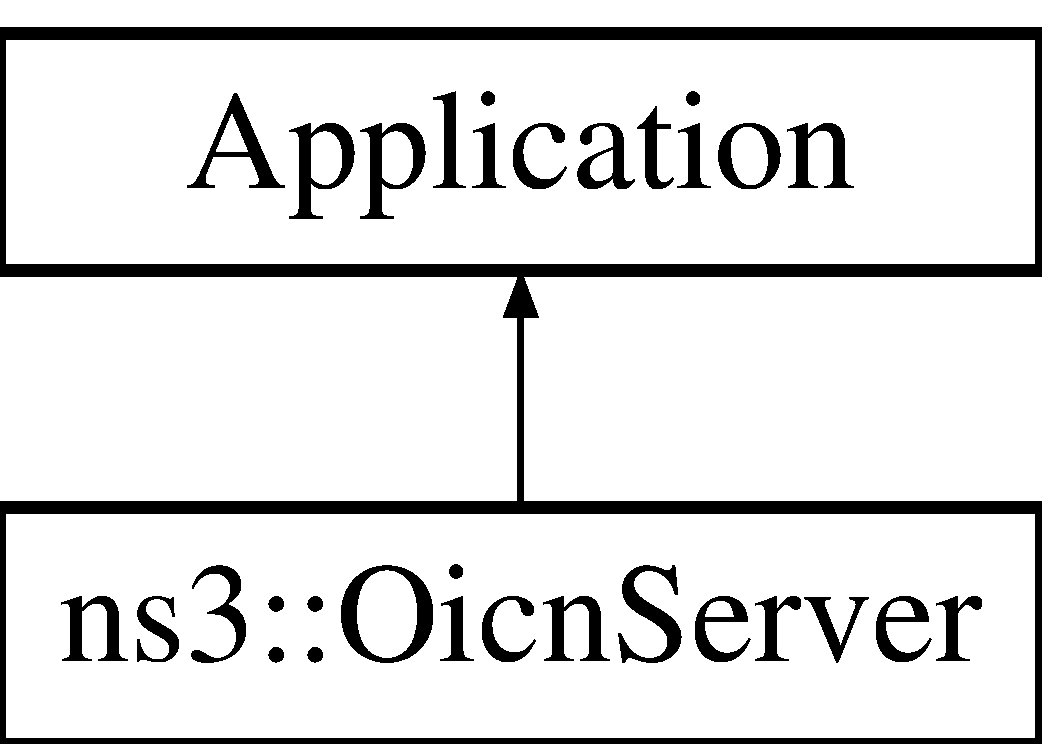
\includegraphics[height=2.000000cm]{classns3_1_1OicnServer}
\end{center}
\end{figure}
\subsection*{Public Member Functions}
\begin{DoxyCompactItemize}
\item 
\hyperlink{classns3_1_1OicnServer_ab9f66365f8d1a5f08e8c049aa9f932ef}{Oicn\-Server} ()
\item 
virtual \hyperlink{classns3_1_1OicnServer_ab897c892c1bad60b83f770a53e76547e}{$\sim$\-Oicn\-Server} (void)
\item 
void \hyperlink{classns3_1_1OicnServer_a61860ecd2544eb4e7774c7c2c19da63c}{Set\-Content} (std\-::vector$<$ int $>$ index)
\begin{DoxyCompactList}\small\item\em During initialisation of server, it sets the content that server will contain. \hyperlink{classns3_1_1Content}{Content} list will remain same during the simulation. \end{DoxyCompactList}\item 
Ptr$<$ Packet $>$ \hyperlink{classns3_1_1OicnServer_a1813b07463e62f0c011a5ab169174c94}{Get\-Content} (std\-::string name)
\begin{DoxyCompactList}\small\item\em It retrieves the content corresponding to the name, passed as the parameter to the function. \end{DoxyCompactList}\item 
Ptr$<$ Packet $>$ \hyperlink{classns3_1_1OicnServer_ae543f14a173b0e294a78694f1f91f15f}{Construct\-Sublayer} (Ptr$<$ Packet $>$ packet, std\-::string name)
\begin{DoxyCompactList}\small\item\em Construct the sublayer header. \end{DoxyCompactList}\item 
void \hyperlink{classns3_1_1OicnServer_a8dd7f5f546baf72d2eeef2ba78c3b797}{Send\-To\-Client} (uint32\-\_\-t client\-Address, std\-::string name)
\begin{DoxyCompactList}\small\item\em Send the content to client. \end{DoxyCompactList}\item 
void \hyperlink{classns3_1_1OicnServer_abd1ea8c1e1332d232c2a2dbc559ea769}{Read\-Packet} (Ptr$<$ Packet $>$ packet, Ipv4\-Address sender\-Address, uint16\-\_\-t sender\-Port)
\begin{DoxyCompactList}\small\item\em Read the packet received at I\-C\-N Manager port i.\-e. 89. \end{DoxyCompactList}\item 
void \hyperlink{classns3_1_1OicnServer_af9a0c2a5aae516f33ae3a6a452b6e61c}{Send\-Ack\-To\-Icn\-Manager} (Ipv4\-Address icn\-Manager\-Ipv4\-Address, uint16\-\_\-t icn\-Manager\-Port, \hyperlink{classns3_1_1DnsPlusQuestionHeader}{Dns\-Plus\-Question\-Header} dns\-Plus\-Question\-Header, \hyperlink{classns3_1_1DnsPlusHeader}{Dns\-Plus\-Header} dns\-Plus\-Header, \hyperlink{classns3_1_1OicnHeader}{Oicn\-Header} oicn\-Header)
\begin{DoxyCompactList}\small\item\em After receiving the content request from the I\-C\-N Manager, it send back the A\-C\-K of same to I\-C\-N Manager. \end{DoxyCompactList}\end{DoxyCompactItemize}
\subsection*{Static Public Member Functions}
\begin{DoxyCompactItemize}
\item 
static Type\-Id \hyperlink{classns3_1_1OicnServer_a6feccce194eec32aeeaaed73b215c7ec}{Get\-Type\-Id} (void)
\begin{DoxyCompactList}\small\item\em Get the type I\-D. \end{DoxyCompactList}\end{DoxyCompactItemize}
\subsection*{Protected Member Functions}
\begin{DoxyCompactItemize}
\item 
virtual void \hyperlink{classns3_1_1OicnServer_a6a2cf9407f2c0d0168d1f2d99c57ba6e}{Do\-Dispose} (void)
\end{DoxyCompactItemize}
\subsection*{Private Member Functions}
\begin{DoxyCompactItemize}
\item 
void \hyperlink{classns3_1_1OicnServer_acc544f5a8c2941ebbec576dd87ebbd4b}{Handle\-Read\-Icn\-Manger} (Ptr$<$ Socket $>$ socket)
\begin{DoxyCompactList}\small\item\em Handle a packet reception from I\-C\-N Manager port (36). This function is called by lower layers. \end{DoxyCompactList}\item 
virtual void \hyperlink{classns3_1_1OicnServer_a185a5fb39786caf3f89a65b08f61a6e8}{Start\-Application} (void)
\item 
virtual void \hyperlink{classns3_1_1OicnServer_a12256e51cce0c25a66eef8cc256e367e}{Stop\-Application} (void)
\end{DoxyCompactItemize}
\subsection*{Private Attributes}
\begin{DoxyCompactItemize}
\item 
boost\-::unordered\-\_\-map\\*
$<$ std\-::string, std\-::string $>$ \hyperlink{classns3_1_1OicnServer_ae9c0c07d3749a24b15ad2cd3e13c52a6}{server\-\_\-content}
\begin{DoxyCompactList}\small\item\em It contain name and corresponding content. \end{DoxyCompactList}\item 
Ptr$<$ Socket $>$ \hyperlink{classns3_1_1OicnServer_ab5844e0fda8496f62cb0bd472a1e4783}{m\-\_\-socket}
\begin{DoxyCompactList}\small\item\em socket \end{DoxyCompactList}\item 
Ptr$<$ Socket $>$ \hyperlink{classns3_1_1OicnServer_a836b1c3feef3d7946fd187dec6e4f229}{m\-\_\-socket\-Icn\-Manager}
\begin{DoxyCompactList}\small\item\em socket connected to I\-C\-N Manager port 36 \end{DoxyCompactList}\item 
uint16\-\_\-t \hyperlink{classns3_1_1OicnServer_af323ee83ebbb895c021b3ba2eadae2cc}{m\-\_\-port}
\begin{DoxyCompactList}\small\item\em port at which server listens it defined as 89 \end{DoxyCompactList}\item 
uint16\-\_\-t \hyperlink{classns3_1_1OicnServer_a3c7e8287c7efc4790e2a83c67163daca}{m\-\_\-client\-Port}
\begin{DoxyCompactList}\small\item\em port at which client will listen to the request, here defined as 26 \end{DoxyCompactList}\end{DoxyCompactItemize}


\subsection{Detailed Description}
O\-I\-C\-N Server Application, it accept request of content from I\-C\-N Manager and send to the client. 

\subsection{Constructor \& Destructor Documentation}
\hypertarget{classns3_1_1OicnServer_ab9f66365f8d1a5f08e8c049aa9f932ef}{\index{ns3\-::\-Oicn\-Server@{ns3\-::\-Oicn\-Server}!Oicn\-Server@{Oicn\-Server}}
\index{Oicn\-Server@{Oicn\-Server}!ns3::OicnServer@{ns3\-::\-Oicn\-Server}}
\subsubsection[{Oicn\-Server}]{\setlength{\rightskip}{0pt plus 5cm}ns3\-::\-Oicn\-Server\-::\-Oicn\-Server (
\begin{DoxyParamCaption}
{}
\end{DoxyParamCaption}
)}}\label{classns3_1_1OicnServer_ab9f66365f8d1a5f08e8c049aa9f932ef}
\hypertarget{classns3_1_1OicnServer_ab897c892c1bad60b83f770a53e76547e}{\index{ns3\-::\-Oicn\-Server@{ns3\-::\-Oicn\-Server}!$\sim$\-Oicn\-Server@{$\sim$\-Oicn\-Server}}
\index{$\sim$\-Oicn\-Server@{$\sim$\-Oicn\-Server}!ns3::OicnServer@{ns3\-::\-Oicn\-Server}}
\subsubsection[{$\sim$\-Oicn\-Server}]{\setlength{\rightskip}{0pt plus 5cm}ns3\-::\-Oicn\-Server\-::$\sim$\-Oicn\-Server (
\begin{DoxyParamCaption}
\item[{void}]{}
\end{DoxyParamCaption}
)\hspace{0.3cm}{\ttfamily [virtual]}}}\label{classns3_1_1OicnServer_ab897c892c1bad60b83f770a53e76547e}


\subsection{Member Function Documentation}
\hypertarget{classns3_1_1OicnServer_ae543f14a173b0e294a78694f1f91f15f}{\index{ns3\-::\-Oicn\-Server@{ns3\-::\-Oicn\-Server}!Construct\-Sublayer@{Construct\-Sublayer}}
\index{Construct\-Sublayer@{Construct\-Sublayer}!ns3::OicnServer@{ns3\-::\-Oicn\-Server}}
\subsubsection[{Construct\-Sublayer}]{\setlength{\rightskip}{0pt plus 5cm}Ptr$<$ Packet $>$ ns3\-::\-Oicn\-Server\-::\-Construct\-Sublayer (
\begin{DoxyParamCaption}
\item[{Ptr$<$ Packet $>$}]{packet, }
\item[{std\-::string}]{name}
\end{DoxyParamCaption}
)}}\label{classns3_1_1OicnServer_ae543f14a173b0e294a78694f1f91f15f}


Construct the sublayer header. 


\begin{DoxyParams}{Parameters}
{\em packet} & packet constructed by application layer \\
\hline
{\em name} & name of the content \\
\hline
\end{DoxyParams}
\begin{DoxyReturn}{Returns}
packet constructed after adding sublayer 
\end{DoxyReturn}
\hypertarget{classns3_1_1OicnServer_a6a2cf9407f2c0d0168d1f2d99c57ba6e}{\index{ns3\-::\-Oicn\-Server@{ns3\-::\-Oicn\-Server}!Do\-Dispose@{Do\-Dispose}}
\index{Do\-Dispose@{Do\-Dispose}!ns3::OicnServer@{ns3\-::\-Oicn\-Server}}
\subsubsection[{Do\-Dispose}]{\setlength{\rightskip}{0pt plus 5cm}void ns3\-::\-Oicn\-Server\-::\-Do\-Dispose (
\begin{DoxyParamCaption}
\item[{void}]{}
\end{DoxyParamCaption}
)\hspace{0.3cm}{\ttfamily [protected]}, {\ttfamily [virtual]}}}\label{classns3_1_1OicnServer_a6a2cf9407f2c0d0168d1f2d99c57ba6e}
\hypertarget{classns3_1_1OicnServer_a1813b07463e62f0c011a5ab169174c94}{\index{ns3\-::\-Oicn\-Server@{ns3\-::\-Oicn\-Server}!Get\-Content@{Get\-Content}}
\index{Get\-Content@{Get\-Content}!ns3::OicnServer@{ns3\-::\-Oicn\-Server}}
\subsubsection[{Get\-Content}]{\setlength{\rightskip}{0pt plus 5cm}Ptr$<$ Packet $>$ ns3\-::\-Oicn\-Server\-::\-Get\-Content (
\begin{DoxyParamCaption}
\item[{std\-::string}]{name}
\end{DoxyParamCaption}
)}}\label{classns3_1_1OicnServer_a1813b07463e62f0c011a5ab169174c94}


It retrieves the content corresponding to the name, passed as the parameter to the function. 


\begin{DoxyParams}{Parameters}
{\em name} & name of the content \\
\hline
\end{DoxyParams}
\begin{DoxyReturn}{Returns}
packet containing the content, corresponding to the name mentioned in the parameter 
\end{DoxyReturn}
\hypertarget{classns3_1_1OicnServer_a6feccce194eec32aeeaaed73b215c7ec}{\index{ns3\-::\-Oicn\-Server@{ns3\-::\-Oicn\-Server}!Get\-Type\-Id@{Get\-Type\-Id}}
\index{Get\-Type\-Id@{Get\-Type\-Id}!ns3::OicnServer@{ns3\-::\-Oicn\-Server}}
\subsubsection[{Get\-Type\-Id}]{\setlength{\rightskip}{0pt plus 5cm}Type\-Id ns3\-::\-Oicn\-Server\-::\-Get\-Type\-Id (
\begin{DoxyParamCaption}
\item[{void}]{}
\end{DoxyParamCaption}
)\hspace{0.3cm}{\ttfamily [static]}}}\label{classns3_1_1OicnServer_a6feccce194eec32aeeaaed73b215c7ec}


Get the type I\-D. 

\begin{DoxyReturn}{Returns}
the object Type\-Id 
\end{DoxyReturn}
\hypertarget{classns3_1_1OicnServer_acc544f5a8c2941ebbec576dd87ebbd4b}{\index{ns3\-::\-Oicn\-Server@{ns3\-::\-Oicn\-Server}!Handle\-Read\-Icn\-Manger@{Handle\-Read\-Icn\-Manger}}
\index{Handle\-Read\-Icn\-Manger@{Handle\-Read\-Icn\-Manger}!ns3::OicnServer@{ns3\-::\-Oicn\-Server}}
\subsubsection[{Handle\-Read\-Icn\-Manger}]{\setlength{\rightskip}{0pt plus 5cm}void ns3\-::\-Oicn\-Server\-::\-Handle\-Read\-Icn\-Manger (
\begin{DoxyParamCaption}
\item[{Ptr$<$ Socket $>$}]{socket}
\end{DoxyParamCaption}
)\hspace{0.3cm}{\ttfamily [private]}}}\label{classns3_1_1OicnServer_acc544f5a8c2941ebbec576dd87ebbd4b}


Handle a packet reception from I\-C\-N Manager port (36). This function is called by lower layers. 


\begin{DoxyParams}{Parameters}
{\em socket} & the socket the packet was received to \\
\hline
\end{DoxyParams}
\hypertarget{classns3_1_1OicnServer_abd1ea8c1e1332d232c2a2dbc559ea769}{\index{ns3\-::\-Oicn\-Server@{ns3\-::\-Oicn\-Server}!Read\-Packet@{Read\-Packet}}
\index{Read\-Packet@{Read\-Packet}!ns3::OicnServer@{ns3\-::\-Oicn\-Server}}
\subsubsection[{Read\-Packet}]{\setlength{\rightskip}{0pt plus 5cm}void ns3\-::\-Oicn\-Server\-::\-Read\-Packet (
\begin{DoxyParamCaption}
\item[{Ptr$<$ Packet $>$}]{packet, }
\item[{Ipv4\-Address}]{sender\-Address, }
\item[{uint16\-\_\-t}]{sender\-Port}
\end{DoxyParamCaption}
)}}\label{classns3_1_1OicnServer_abd1ea8c1e1332d232c2a2dbc559ea769}


Read the packet received at I\-C\-N Manager port i.\-e. 89. 


\begin{DoxyParams}{Parameters}
{\em packet} & packet received at I\-C\-N Manager port \\
\hline
{\em sender\-Address} & Ipv4 address of the sender \\
\hline
{\em sender\-Port} & port of the sender \\
\hline
\end{DoxyParams}
\hypertarget{classns3_1_1OicnServer_af9a0c2a5aae516f33ae3a6a452b6e61c}{\index{ns3\-::\-Oicn\-Server@{ns3\-::\-Oicn\-Server}!Send\-Ack\-To\-Icn\-Manager@{Send\-Ack\-To\-Icn\-Manager}}
\index{Send\-Ack\-To\-Icn\-Manager@{Send\-Ack\-To\-Icn\-Manager}!ns3::OicnServer@{ns3\-::\-Oicn\-Server}}
\subsubsection[{Send\-Ack\-To\-Icn\-Manager}]{\setlength{\rightskip}{0pt plus 5cm}void ns3\-::\-Oicn\-Server\-::\-Send\-Ack\-To\-Icn\-Manager (
\begin{DoxyParamCaption}
\item[{Ipv4\-Address}]{icn\-Manager\-Ipv4\-Address, }
\item[{uint16\-\_\-t}]{icn\-Manager\-Port, }
\item[{{\bf Dns\-Plus\-Question\-Header}}]{dns\-Plus\-Question\-Header, }
\item[{{\bf Dns\-Plus\-Header}}]{dns\-Plus\-Header, }
\item[{{\bf Oicn\-Header}}]{oicn\-Header}
\end{DoxyParamCaption}
)}}\label{classns3_1_1OicnServer_af9a0c2a5aae516f33ae3a6a452b6e61c}


After receiving the content request from the I\-C\-N Manager, it send back the A\-C\-K of same to I\-C\-N Manager. 


\begin{DoxyParams}{Parameters}
{\em icn\-Manager\-Ipv4\-Address} & I\-C\-N Manager Ipv4 address to which A\-C\-K has to be sent \\
\hline
{\em icn\-Manager\-Port} & I\-C\-N Manager port at which A\-C\-K has to be sent \\
\hline
{\em dns\-Plus\-Question\-Header} & dns Plus Question header section of the packet \\
\hline
{\em dns\-Plus\-Header} & dns Plus header section of the packet \\
\hline
{\em oicn\-Header} & oicn header section of the packet \\
\hline
\end{DoxyParams}
\hypertarget{classns3_1_1OicnServer_a8dd7f5f546baf72d2eeef2ba78c3b797}{\index{ns3\-::\-Oicn\-Server@{ns3\-::\-Oicn\-Server}!Send\-To\-Client@{Send\-To\-Client}}
\index{Send\-To\-Client@{Send\-To\-Client}!ns3::OicnServer@{ns3\-::\-Oicn\-Server}}
\subsubsection[{Send\-To\-Client}]{\setlength{\rightskip}{0pt plus 5cm}void ns3\-::\-Oicn\-Server\-::\-Send\-To\-Client (
\begin{DoxyParamCaption}
\item[{uint32\-\_\-t}]{client\-Address, }
\item[{std\-::string}]{name}
\end{DoxyParamCaption}
)}}\label{classns3_1_1OicnServer_a8dd7f5f546baf72d2eeef2ba78c3b797}


Send the content to client. 


\begin{DoxyParams}{Parameters}
{\em client\-Address} & address of the client \\
\hline
{\em name} & name of the content \\
\hline
\end{DoxyParams}
\hypertarget{classns3_1_1OicnServer_a61860ecd2544eb4e7774c7c2c19da63c}{\index{ns3\-::\-Oicn\-Server@{ns3\-::\-Oicn\-Server}!Set\-Content@{Set\-Content}}
\index{Set\-Content@{Set\-Content}!ns3::OicnServer@{ns3\-::\-Oicn\-Server}}
\subsubsection[{Set\-Content}]{\setlength{\rightskip}{0pt plus 5cm}void ns3\-::\-Oicn\-Server\-::\-Set\-Content (
\begin{DoxyParamCaption}
\item[{std\-::vector$<$ int $>$}]{index}
\end{DoxyParamCaption}
)}}\label{classns3_1_1OicnServer_a61860ecd2544eb4e7774c7c2c19da63c}


During initialisation of server, it sets the content that server will contain. \hyperlink{classns3_1_1Content}{Content} list will remain same during the simulation. 


\begin{DoxyParams}{Parameters}
{\em index} & index of content, which the server will contain \\
\hline
\end{DoxyParams}
\hypertarget{classns3_1_1OicnServer_a185a5fb39786caf3f89a65b08f61a6e8}{\index{ns3\-::\-Oicn\-Server@{ns3\-::\-Oicn\-Server}!Start\-Application@{Start\-Application}}
\index{Start\-Application@{Start\-Application}!ns3::OicnServer@{ns3\-::\-Oicn\-Server}}
\subsubsection[{Start\-Application}]{\setlength{\rightskip}{0pt plus 5cm}void ns3\-::\-Oicn\-Server\-::\-Start\-Application (
\begin{DoxyParamCaption}
\item[{void}]{}
\end{DoxyParamCaption}
)\hspace{0.3cm}{\ttfamily [private]}, {\ttfamily [virtual]}}}\label{classns3_1_1OicnServer_a185a5fb39786caf3f89a65b08f61a6e8}
\hypertarget{classns3_1_1OicnServer_a12256e51cce0c25a66eef8cc256e367e}{\index{ns3\-::\-Oicn\-Server@{ns3\-::\-Oicn\-Server}!Stop\-Application@{Stop\-Application}}
\index{Stop\-Application@{Stop\-Application}!ns3::OicnServer@{ns3\-::\-Oicn\-Server}}
\subsubsection[{Stop\-Application}]{\setlength{\rightskip}{0pt plus 5cm}void ns3\-::\-Oicn\-Server\-::\-Stop\-Application (
\begin{DoxyParamCaption}
\item[{void}]{}
\end{DoxyParamCaption}
)\hspace{0.3cm}{\ttfamily [private]}, {\ttfamily [virtual]}}}\label{classns3_1_1OicnServer_a12256e51cce0c25a66eef8cc256e367e}


\subsection{Member Data Documentation}
\hypertarget{classns3_1_1OicnServer_a3c7e8287c7efc4790e2a83c67163daca}{\index{ns3\-::\-Oicn\-Server@{ns3\-::\-Oicn\-Server}!m\-\_\-client\-Port@{m\-\_\-client\-Port}}
\index{m\-\_\-client\-Port@{m\-\_\-client\-Port}!ns3::OicnServer@{ns3\-::\-Oicn\-Server}}
\subsubsection[{m\-\_\-client\-Port}]{\setlength{\rightskip}{0pt plus 5cm}uint16\-\_\-t ns3\-::\-Oicn\-Server\-::m\-\_\-client\-Port\hspace{0.3cm}{\ttfamily [private]}}}\label{classns3_1_1OicnServer_a3c7e8287c7efc4790e2a83c67163daca}


port at which client will listen to the request, here defined as 26 

\hypertarget{classns3_1_1OicnServer_af323ee83ebbb895c021b3ba2eadae2cc}{\index{ns3\-::\-Oicn\-Server@{ns3\-::\-Oicn\-Server}!m\-\_\-port@{m\-\_\-port}}
\index{m\-\_\-port@{m\-\_\-port}!ns3::OicnServer@{ns3\-::\-Oicn\-Server}}
\subsubsection[{m\-\_\-port}]{\setlength{\rightskip}{0pt plus 5cm}uint16\-\_\-t ns3\-::\-Oicn\-Server\-::m\-\_\-port\hspace{0.3cm}{\ttfamily [private]}}}\label{classns3_1_1OicnServer_af323ee83ebbb895c021b3ba2eadae2cc}


port at which server listens it defined as 89 

\hypertarget{classns3_1_1OicnServer_ab5844e0fda8496f62cb0bd472a1e4783}{\index{ns3\-::\-Oicn\-Server@{ns3\-::\-Oicn\-Server}!m\-\_\-socket@{m\-\_\-socket}}
\index{m\-\_\-socket@{m\-\_\-socket}!ns3::OicnServer@{ns3\-::\-Oicn\-Server}}
\subsubsection[{m\-\_\-socket}]{\setlength{\rightskip}{0pt plus 5cm}Ptr$<$Socket$>$ ns3\-::\-Oicn\-Server\-::m\-\_\-socket\hspace{0.3cm}{\ttfamily [private]}}}\label{classns3_1_1OicnServer_ab5844e0fda8496f62cb0bd472a1e4783}


socket 

\hypertarget{classns3_1_1OicnServer_a836b1c3feef3d7946fd187dec6e4f229}{\index{ns3\-::\-Oicn\-Server@{ns3\-::\-Oicn\-Server}!m\-\_\-socket\-Icn\-Manager@{m\-\_\-socket\-Icn\-Manager}}
\index{m\-\_\-socket\-Icn\-Manager@{m\-\_\-socket\-Icn\-Manager}!ns3::OicnServer@{ns3\-::\-Oicn\-Server}}
\subsubsection[{m\-\_\-socket\-Icn\-Manager}]{\setlength{\rightskip}{0pt plus 5cm}Ptr$<$Socket$>$ ns3\-::\-Oicn\-Server\-::m\-\_\-socket\-Icn\-Manager\hspace{0.3cm}{\ttfamily [private]}}}\label{classns3_1_1OicnServer_a836b1c3feef3d7946fd187dec6e4f229}


socket connected to I\-C\-N Manager port 36 

\hypertarget{classns3_1_1OicnServer_ae9c0c07d3749a24b15ad2cd3e13c52a6}{\index{ns3\-::\-Oicn\-Server@{ns3\-::\-Oicn\-Server}!server\-\_\-content@{server\-\_\-content}}
\index{server\-\_\-content@{server\-\_\-content}!ns3::OicnServer@{ns3\-::\-Oicn\-Server}}
\subsubsection[{server\-\_\-content}]{\setlength{\rightskip}{0pt plus 5cm}boost\-::unordered\-\_\-map$<$std\-::string, std\-::string$>$ ns3\-::\-Oicn\-Server\-::server\-\_\-content\hspace{0.3cm}{\ttfamily [private]}}}\label{classns3_1_1OicnServer_ae9c0c07d3749a24b15ad2cd3e13c52a6}


It contain name and corresponding content. 



The documentation for this class was generated from the following files\-:\begin{DoxyCompactItemize}
\item 
model/\hyperlink{oicn-server-application_8h}{oicn-\/server-\/application.\-h}\item 
model/\hyperlink{oicn-server-application_8cc}{oicn-\/server-\/application.\-cc}\end{DoxyCompactItemize}

\hypertarget{classns3_1_1OicnServerHelper}{\section{ns3\-:\-:Oicn\-Server\-Helper Class Reference}
\label{classns3_1_1OicnServerHelper}\index{ns3\-::\-Oicn\-Server\-Helper@{ns3\-::\-Oicn\-Server\-Helper}}
}


Create a O\-I\-C\-N Server application. I\-C\-N Manager direct O\-I\-C\-N server to send requested content to O\-I\-C\-N client.  




{\ttfamily \#include $<$oicn-\/application-\/helper.\-h$>$}

\subsection*{Public Member Functions}
\begin{DoxyCompactItemize}
\item 
\hyperlink{classns3_1_1OicnServerHelper_a998b6d70d51296b555b21db53495fa06}{Oicn\-Server\-Helper} ()
\item 
Application\-Container \hyperlink{classns3_1_1OicnServerHelper_a4b67e200abe0195e41e9d90fe7d39bbd}{Install} (Ptr$<$ Node $>$ node, std\-::vector$<$ int $>$ index) const 
\item 
Application\-Container \hyperlink{classns3_1_1OicnServerHelper_aea4f4451e7c402188d9420bd1651d353}{Install} (Node\-Container c, std\-::vector$<$ int $>$ index) const 
\end{DoxyCompactItemize}
\subsection*{Private Member Functions}
\begin{DoxyCompactItemize}
\item 
Application\-Container \hyperlink{classns3_1_1OicnServerHelper_ab941edf2e4f5d21a605234c5641c389e}{Install\-Priv} (Ptr$<$ Node $>$ node, std\-::vector$<$ int $>$ index) const 
\end{DoxyCompactItemize}
\subsection*{Private Attributes}
\begin{DoxyCompactItemize}
\item 
Object\-Factory \hyperlink{classns3_1_1OicnServerHelper_a19cdffceba4d5dfc156b3f1bf18e2531}{m\-\_\-factory}
\begin{DoxyCompactList}\small\item\em Object factory. \end{DoxyCompactList}\end{DoxyCompactItemize}


\subsection{Detailed Description}
Create a O\-I\-C\-N Server application. I\-C\-N Manager direct O\-I\-C\-N server to send requested content to O\-I\-C\-N client. 

\subsection{Constructor \& Destructor Documentation}
\hypertarget{classns3_1_1OicnServerHelper_a998b6d70d51296b555b21db53495fa06}{\index{ns3\-::\-Oicn\-Server\-Helper@{ns3\-::\-Oicn\-Server\-Helper}!Oicn\-Server\-Helper@{Oicn\-Server\-Helper}}
\index{Oicn\-Server\-Helper@{Oicn\-Server\-Helper}!ns3::OicnServerHelper@{ns3\-::\-Oicn\-Server\-Helper}}
\subsubsection[{Oicn\-Server\-Helper}]{\setlength{\rightskip}{0pt plus 5cm}ns3\-::\-Oicn\-Server\-Helper\-::\-Oicn\-Server\-Helper (
\begin{DoxyParamCaption}
{}
\end{DoxyParamCaption}
)}}\label{classns3_1_1OicnServerHelper_a998b6d70d51296b555b21db53495fa06}


\subsection{Member Function Documentation}
\hypertarget{classns3_1_1OicnServerHelper_a4b67e200abe0195e41e9d90fe7d39bbd}{\index{ns3\-::\-Oicn\-Server\-Helper@{ns3\-::\-Oicn\-Server\-Helper}!Install@{Install}}
\index{Install@{Install}!ns3::OicnServerHelper@{ns3\-::\-Oicn\-Server\-Helper}}
\subsubsection[{Install}]{\setlength{\rightskip}{0pt plus 5cm}Application\-Container ns3\-::\-Oicn\-Server\-Helper\-::\-Install (
\begin{DoxyParamCaption}
\item[{Ptr$<$ Node $>$}]{node, }
\item[{std\-::vector$<$ int $>$}]{index}
\end{DoxyParamCaption}
) const}}\label{classns3_1_1OicnServerHelper_a4b67e200abe0195e41e9d90fe7d39bbd}
Create an \hyperlink{classns3_1_1OicnServer}{Oicn\-Server} Application having content specified by indices on the specified node.


\begin{DoxyParams}{Parameters}
{\em node} & The node on which to create the Application. The node is specified by a Ptr$<$\-Node$>$. \\
\hline
{\em index} & vector containing the indices of the content \\
\hline
\end{DoxyParams}
\begin{DoxyReturn}{Returns}
an Application\-Container holding the Application created 
\end{DoxyReturn}
\hypertarget{classns3_1_1OicnServerHelper_aea4f4451e7c402188d9420bd1651d353}{\index{ns3\-::\-Oicn\-Server\-Helper@{ns3\-::\-Oicn\-Server\-Helper}!Install@{Install}}
\index{Install@{Install}!ns3::OicnServerHelper@{ns3\-::\-Oicn\-Server\-Helper}}
\subsubsection[{Install}]{\setlength{\rightskip}{0pt plus 5cm}Application\-Container ns3\-::\-Oicn\-Server\-Helper\-::\-Install (
\begin{DoxyParamCaption}
\item[{Node\-Container}]{c, }
\item[{std\-::vector$<$ int $>$}]{index}
\end{DoxyParamCaption}
) const}}\label{classns3_1_1OicnServerHelper_aea4f4451e7c402188d9420bd1651d353}
Create an \hyperlink{classns3_1_1OicnServer}{Oicn\-Server} Application having content specified by indices on the specified Node.


\begin{DoxyParams}{Parameters}
{\em c} & The nodes on which to create the Applications. The nodes are specified by a Node\-Container. \\
\hline
{\em index} & vector containing the indices of the content \\
\hline
\end{DoxyParams}
\begin{DoxyReturn}{Returns}
an Application\-Container holding the Application created 
\end{DoxyReturn}
\hypertarget{classns3_1_1OicnServerHelper_ab941edf2e4f5d21a605234c5641c389e}{\index{ns3\-::\-Oicn\-Server\-Helper@{ns3\-::\-Oicn\-Server\-Helper}!Install\-Priv@{Install\-Priv}}
\index{Install\-Priv@{Install\-Priv}!ns3::OicnServerHelper@{ns3\-::\-Oicn\-Server\-Helper}}
\subsubsection[{Install\-Priv}]{\setlength{\rightskip}{0pt plus 5cm}Application\-Container ns3\-::\-Oicn\-Server\-Helper\-::\-Install\-Priv (
\begin{DoxyParamCaption}
\item[{Ptr$<$ Node $>$}]{node, }
\item[{std\-::vector$<$ int $>$}]{index}
\end{DoxyParamCaption}
) const\hspace{0.3cm}{\ttfamily [private]}}}\label{classns3_1_1OicnServerHelper_ab941edf2e4f5d21a605234c5641c389e}
Install an \hyperlink{classns3_1_1OicnServer}{Oicn\-Server} on the node 
\begin{DoxyParams}{Parameters}
{\em node} & The node on which an \hyperlink{classns3_1_1OicnServer}{Oicn\-Server} will be installed. \\
\hline
{\em index} & vector containing the indices of the content \\
\hline
\end{DoxyParams}
\begin{DoxyReturn}{Returns}
an Application\-Container holding the Application created 
\end{DoxyReturn}


\subsection{Member Data Documentation}
\hypertarget{classns3_1_1OicnServerHelper_a19cdffceba4d5dfc156b3f1bf18e2531}{\index{ns3\-::\-Oicn\-Server\-Helper@{ns3\-::\-Oicn\-Server\-Helper}!m\-\_\-factory@{m\-\_\-factory}}
\index{m\-\_\-factory@{m\-\_\-factory}!ns3::OicnServerHelper@{ns3\-::\-Oicn\-Server\-Helper}}
\subsubsection[{m\-\_\-factory}]{\setlength{\rightskip}{0pt plus 5cm}Object\-Factory ns3\-::\-Oicn\-Server\-Helper\-::m\-\_\-factory\hspace{0.3cm}{\ttfamily [private]}}}\label{classns3_1_1OicnServerHelper_a19cdffceba4d5dfc156b3f1bf18e2531}


Object factory. 



The documentation for this class was generated from the following files\-:\begin{DoxyCompactItemize}
\item 
helper/\hyperlink{oicn-application-helper_8h}{oicn-\/application-\/helper.\-h}\item 
helper/\hyperlink{oicn-application-helper_8cc}{oicn-\/application-\/helper.\-cc}\end{DoxyCompactItemize}

\hypertarget{classOIcnTestCase1}{\section{O\-Icn\-Test\-Case1 Class Reference}
\label{classOIcnTestCase1}\index{O\-Icn\-Test\-Case1@{O\-Icn\-Test\-Case1}}
}
Inheritance diagram for O\-Icn\-Test\-Case1\-:\begin{figure}[H]
\begin{center}
\leavevmode
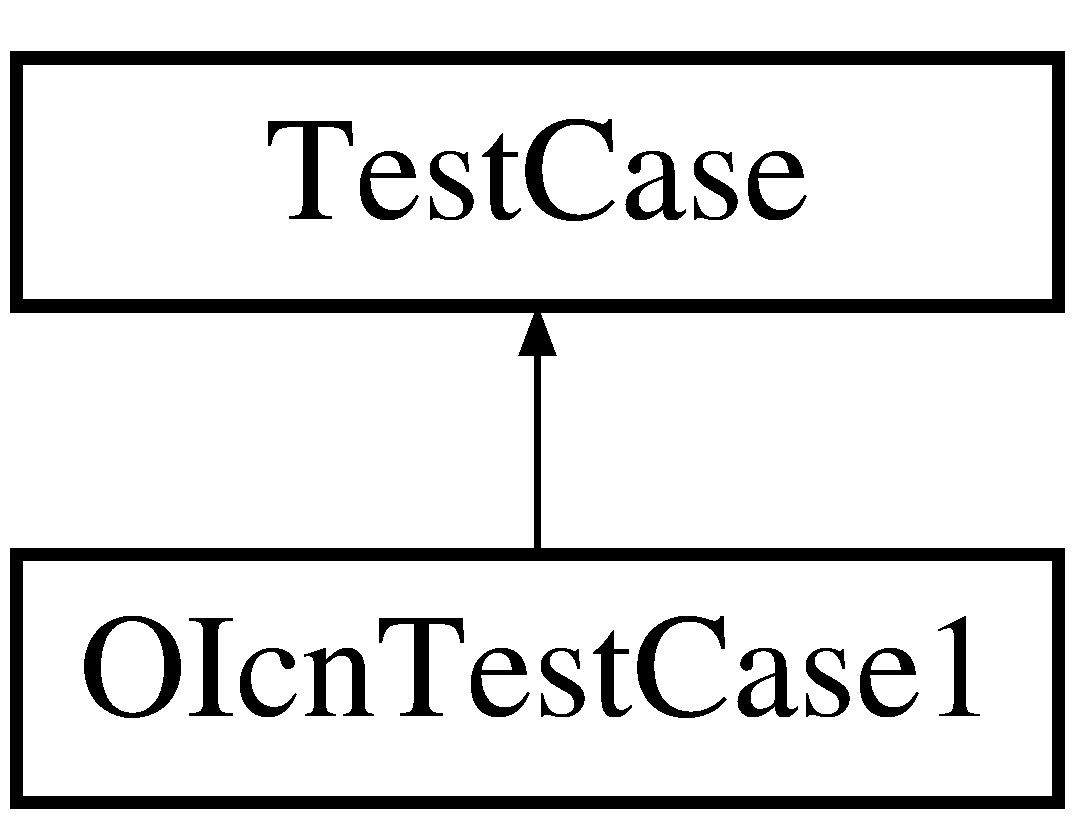
\includegraphics[height=2.000000cm]{classOIcnTestCase1}
\end{center}
\end{figure}
\subsection*{Public Member Functions}
\begin{DoxyCompactItemize}
\item 
\hyperlink{classOIcnTestCase1_aa0896d0862938fa8d3c95a0a2f9975c5}{O\-Icn\-Test\-Case1} ()
\item 
virtual \hyperlink{classOIcnTestCase1_add5c4dc2b17a29935529fc70466e2831}{$\sim$\-O\-Icn\-Test\-Case1} ()
\end{DoxyCompactItemize}
\subsection*{Private Member Functions}
\begin{DoxyCompactItemize}
\item 
virtual void \hyperlink{classOIcnTestCase1_af4aeea901fc4edf5f3efb357bf890154}{Do\-Run} (void)
\end{DoxyCompactItemize}


\subsection{Constructor \& Destructor Documentation}
\hypertarget{classOIcnTestCase1_aa0896d0862938fa8d3c95a0a2f9975c5}{\index{O\-Icn\-Test\-Case1@{O\-Icn\-Test\-Case1}!O\-Icn\-Test\-Case1@{O\-Icn\-Test\-Case1}}
\index{O\-Icn\-Test\-Case1@{O\-Icn\-Test\-Case1}!OIcnTestCase1@{O\-Icn\-Test\-Case1}}
\subsubsection[{O\-Icn\-Test\-Case1}]{\setlength{\rightskip}{0pt plus 5cm}O\-Icn\-Test\-Case1\-::\-O\-Icn\-Test\-Case1 (
\begin{DoxyParamCaption}
{}
\end{DoxyParamCaption}
)}}\label{classOIcnTestCase1_aa0896d0862938fa8d3c95a0a2f9975c5}
\hypertarget{classOIcnTestCase1_add5c4dc2b17a29935529fc70466e2831}{\index{O\-Icn\-Test\-Case1@{O\-Icn\-Test\-Case1}!$\sim$\-O\-Icn\-Test\-Case1@{$\sim$\-O\-Icn\-Test\-Case1}}
\index{$\sim$\-O\-Icn\-Test\-Case1@{$\sim$\-O\-Icn\-Test\-Case1}!OIcnTestCase1@{O\-Icn\-Test\-Case1}}
\subsubsection[{$\sim$\-O\-Icn\-Test\-Case1}]{\setlength{\rightskip}{0pt plus 5cm}O\-Icn\-Test\-Case1\-::$\sim$\-O\-Icn\-Test\-Case1 (
\begin{DoxyParamCaption}
{}
\end{DoxyParamCaption}
)\hspace{0.3cm}{\ttfamily [virtual]}}}\label{classOIcnTestCase1_add5c4dc2b17a29935529fc70466e2831}


\subsection{Member Function Documentation}
\hypertarget{classOIcnTestCase1_af4aeea901fc4edf5f3efb357bf890154}{\index{O\-Icn\-Test\-Case1@{O\-Icn\-Test\-Case1}!Do\-Run@{Do\-Run}}
\index{Do\-Run@{Do\-Run}!OIcnTestCase1@{O\-Icn\-Test\-Case1}}
\subsubsection[{Do\-Run}]{\setlength{\rightskip}{0pt plus 5cm}void O\-Icn\-Test\-Case1\-::\-Do\-Run (
\begin{DoxyParamCaption}
\item[{void}]{}
\end{DoxyParamCaption}
)\hspace{0.3cm}{\ttfamily [private]}, {\ttfamily [virtual]}}}\label{classOIcnTestCase1_af4aeea901fc4edf5f3efb357bf890154}


The documentation for this class was generated from the following file\-:\begin{DoxyCompactItemize}
\item 
test/\hyperlink{o-icn-test-suite_8cc}{o-\/icn-\/test-\/suite.\-cc}\end{DoxyCompactItemize}

\hypertarget{classOIcnTestSuite}{\section{O\-Icn\-Test\-Suite Class Reference}
\label{classOIcnTestSuite}\index{O\-Icn\-Test\-Suite@{O\-Icn\-Test\-Suite}}
}
Inheritance diagram for O\-Icn\-Test\-Suite\-:\begin{figure}[H]
\begin{center}
\leavevmode
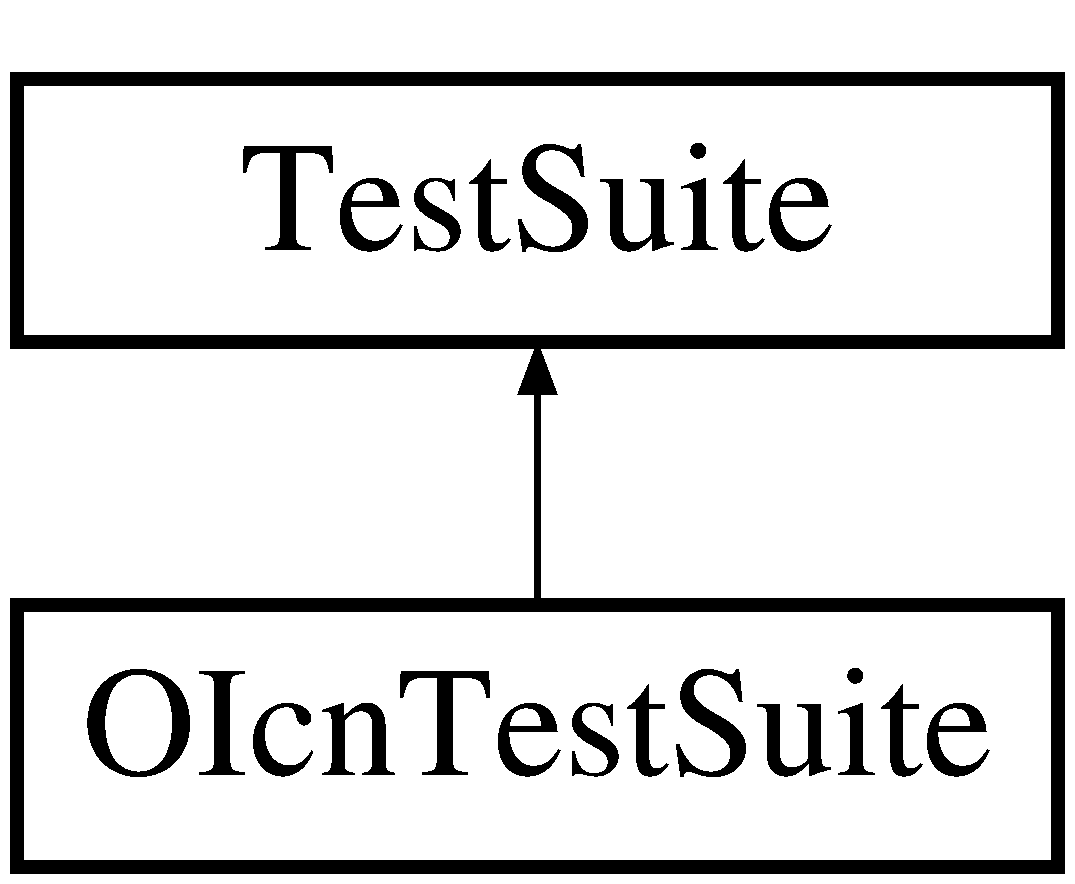
\includegraphics[height=2.000000cm]{classOIcnTestSuite}
\end{center}
\end{figure}
\subsection*{Public Member Functions}
\begin{DoxyCompactItemize}
\item 
\hyperlink{classOIcnTestSuite_a7e6ee1f4e5c7b9495bd62b96ca958229}{O\-Icn\-Test\-Suite} ()
\end{DoxyCompactItemize}


\subsection{Constructor \& Destructor Documentation}
\hypertarget{classOIcnTestSuite_a7e6ee1f4e5c7b9495bd62b96ca958229}{\index{O\-Icn\-Test\-Suite@{O\-Icn\-Test\-Suite}!O\-Icn\-Test\-Suite@{O\-Icn\-Test\-Suite}}
\index{O\-Icn\-Test\-Suite@{O\-Icn\-Test\-Suite}!OIcnTestSuite@{O\-Icn\-Test\-Suite}}
\subsubsection[{O\-Icn\-Test\-Suite}]{\setlength{\rightskip}{0pt plus 5cm}O\-Icn\-Test\-Suite\-::\-O\-Icn\-Test\-Suite (
\begin{DoxyParamCaption}
{}
\end{DoxyParamCaption}
)}}\label{classOIcnTestSuite_a7e6ee1f4e5c7b9495bd62b96ca958229}


The documentation for this class was generated from the following file\-:\begin{DoxyCompactItemize}
\item 
test/\hyperlink{o-icn-test-suite_8cc}{o-\/icn-\/test-\/suite.\-cc}\end{DoxyCompactItemize}

\hypertarget{classns3_1_1OICNZipfClient}{\section{ns3\-:\-:O\-I\-C\-N\-Zipf\-Client Class Reference}
\label{classns3_1_1OICNZipfClient}\index{ns3\-::\-O\-I\-C\-N\-Zipf\-Client@{ns3\-::\-O\-I\-C\-N\-Zipf\-Client}}
}


O\-I\-C\-N Zipf Client application, it generates request for the contents following Zipf-\/\-Mandelbrot Distribution. Here is the explanation of Zipf-\/\-Mandelbrot Distribution\-: \href{http://en.wikipedia.org/wiki/Zipf%E2%80%93Mandelbrot_law}{\tt http\-://en.\-wikipedia.\-org/wiki/\-Zipf\%\-E2\%80\%93\-Mandelbrot\-\_\-law}. Client application send name resolution to I\-C\-N Manager. I\-C\-N Manager do the name resolution and direct source (I\-C\-N router or server) to send the content to the O\-I\-C\-N Zipf Client.  




{\ttfamily \#include $<$oicn-\/zipf-\/client.\-h$>$}

Inheritance diagram for ns3\-:\-:O\-I\-C\-N\-Zipf\-Client\-:\begin{figure}[H]
\begin{center}
\leavevmode
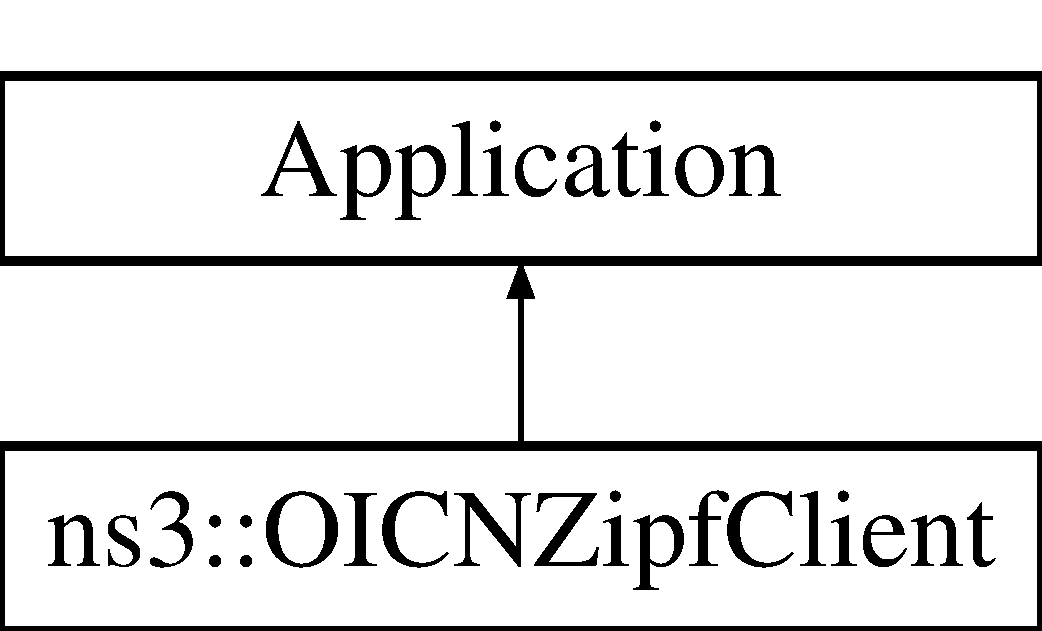
\includegraphics[height=2.000000cm]{classns3_1_1OICNZipfClient}
\end{center}
\end{figure}
\subsection*{Public Member Functions}
\begin{DoxyCompactItemize}
\item 
\hyperlink{classns3_1_1OICNZipfClient_ad408bc6446376318703b8e001d99a97f}{O\-I\-C\-N\-Zipf\-Client} (void)
\item 
virtual \hyperlink{classns3_1_1OICNZipfClient_a3f6cd458cc6a987da49699932c38b9bc}{$\sim$\-O\-I\-C\-N\-Zipf\-Client} (void)
\item 
void \hyperlink{classns3_1_1OICNZipfClient_a61c4940713bdd9363b8313696b2c4ffa}{Set\-Zipf} (std\-::pair$<$ int, int $>$ range)
\begin{DoxyCompactList}\small\item\em Set the range of the index of content. \end{DoxyCompactList}\item 
Ptr$<$ Packet $>$ \hyperlink{classns3_1_1OICNZipfClient_a4a76b1b9373eb3bb7e43970222def563}{Construct\-Sublayer} (Ptr$<$ Packet $>$ packet, std\-::string Name)
\begin{DoxyCompactList}\small\item\em Construct the sublayer header. \end{DoxyCompactList}\item 
Ptr$<$ Packet $>$ \hyperlink{classns3_1_1OICNZipfClient_ade9706357b84a74244249284e6da73cb}{Construct\-Dns\-Plus\-Header} (Ptr$<$ Packet $>$ packet)
\begin{DoxyCompactList}\small\item\em Construct the D\-N\-S Plus header. \end{DoxyCompactList}\item 
Ptr$<$ Packet $>$ \hyperlink{classns3_1_1OICNZipfClient_a966298b46754229776f3536e80fcff57}{Construct\-Dns\-Plus\-Question} (Ptr$<$ Packet $>$ packet, std\-::string name)
\begin{DoxyCompactList}\small\item\em Construct the D\-N\-S Plus Question Section. \end{DoxyCompactList}\end{DoxyCompactItemize}
\subsection*{Static Public Member Functions}
\begin{DoxyCompactItemize}
\item 
static Type\-Id \hyperlink{classns3_1_1OICNZipfClient_afe8d27ae680ce9efbe3006013ff3adf5}{Get\-Type\-Id} (void)
\begin{DoxyCompactList}\small\item\em Get the type I\-D. \end{DoxyCompactList}\end{DoxyCompactItemize}
\subsection*{Protected Member Functions}
\begin{DoxyCompactItemize}
\item 
virtual void \hyperlink{classns3_1_1OICNZipfClient_aa0e32df291032ec158f3bdad7022d7b4}{Do\-Dispose} (void)
\end{DoxyCompactItemize}
\subsection*{Private Member Functions}
\begin{DoxyCompactItemize}
\item 
void \hyperlink{classns3_1_1OICNZipfClient_a82eace7ea478582445022df4add70a9c}{Handle\-Read\-Icn\-Manager} (Ptr$<$ Socket $>$ socket)
\begin{DoxyCompactList}\small\item\em Handle a packet reception from I\-C\-N Manager port (36). This function is called by lower layers. \end{DoxyCompactList}\item 
void \hyperlink{classns3_1_1OICNZipfClient_aee5aa32b3b7d847ac8f01db8439a2b33}{Handle\-Read\-Source} (Ptr$<$ Socket $>$ socket)
\begin{DoxyCompactList}\small\item\em Handle a packet reception from Source port (I\-C\-N Router or Server) (89). This function is called by lower layers. \end{DoxyCompactList}\item 
virtual void \hyperlink{classns3_1_1OICNZipfClient_abe66add9def5db29de9e2fc4b274c636}{Start\-Application} (void)
\item 
virtual void \hyperlink{classns3_1_1OICNZipfClient_af6857512948b5fbcf711f7a126133473}{Stop\-Application} (void)
\item 
int \hyperlink{classns3_1_1OICNZipfClient_a55dcd262453681f5b464cdf732d68ed2}{Get\-Next\-Content\-Index} ()
\begin{DoxyCompactList}\small\item\em Generate the indices of content to be requested following Zipf-\/\-Mandelbrot Distribution. \end{DoxyCompactList}\item 
void \hyperlink{classns3_1_1OICNZipfClient_aa7c04e11ce1f197bd4462e961ef04a2e}{Schedule\-Transmit} (Time dt)
\begin{DoxyCompactList}\small\item\em Schedule the next packet transmission. \end{DoxyCompactList}\item 
void \hyperlink{classns3_1_1OICNZipfClient_a3c656a3d51f7ddc8d6b31fbb88f2a575}{Send} ()
\begin{DoxyCompactList}\small\item\em Send a packet to I\-C\-N Manager. \end{DoxyCompactList}\end{DoxyCompactItemize}
\subsection*{Private Attributes}
\begin{DoxyCompactItemize}
\item 
std\-::pair$<$ uint32\-\_\-t, uint32\-\_\-t $>$ \hyperlink{classns3_1_1OICNZipfClient_a374afd9b3085995e5fc37befbc593925}{m\-\_\-range}
\begin{DoxyCompactList}\small\item\em range of the indices of the contents \end{DoxyCompactList}\item 
uint32\-\_\-t \hyperlink{classns3_1_1OICNZipfClient_ad8cd34cc29d9ff89702f5c805a58aaf4}{m\-\_\-sent}
\begin{DoxyCompactList}\small\item\em counter for sent packets \end{DoxyCompactList}\item 
uint32\-\_\-t \hyperlink{classns3_1_1OICNZipfClient_ab2cc3b1156fb17d67c19e16526696770}{m\-\_\-count}
\begin{DoxyCompactList}\small\item\em the maximum number of packets the application will send \end{DoxyCompactList}\item 
double \hyperlink{classns3_1_1OICNZipfClient_aa56cf1606f17a1753bb4b066f75d5dcc}{m\-\_\-q}
\begin{DoxyCompactList}\small\item\em q in (k+q)$^\wedge$s \end{DoxyCompactList}\item 
double \hyperlink{classns3_1_1OICNZipfClient_a4bf5ef44d4ee8832da331827774bff10}{m\-\_\-s}
\begin{DoxyCompactList}\small\item\em s in (k+q)$^\wedge$s \end{DoxyCompactList}\item 
std\-::vector$<$ double $>$ \hyperlink{classns3_1_1OICNZipfClient_a1dd636e731bbe2b2273970c3e9c191b7}{m\-\_\-\-Pcum}
\begin{DoxyCompactList}\small\item\em cumulative probability \end{DoxyCompactList}\item 
uint32\-\_\-t \hyperlink{classns3_1_1OICNZipfClient_a4146b87daf72c43e4d9f1e288897e30e}{m\-\_\-\-N}
\begin{DoxyCompactList}\small\item\em number of the contents \end{DoxyCompactList}\item 
uint16\-\_\-t \hyperlink{classns3_1_1OICNZipfClient_a9f6a96310cf93dd8233c3f8c7c9bf298}{m\-\_\-port\-Fixed}
\begin{DoxyCompactList}\small\item\em client port is attached with port no 26, it will listen to this port from O\-I\-C\-N Source(\-I\-C\-N router or server) \end{DoxyCompactList}\item 
Ptr$<$ Socket $>$ \hyperlink{classns3_1_1OICNZipfClient_accb08afc8f8218076eaa919743381e79}{m\-\_\-socket\-Icn\-Manager}
\begin{DoxyCompactList}\small\item\em socket associated with I\-C\-N Manager \end{DoxyCompactList}\item 
Ptr$<$ Socket $>$ \hyperlink{classns3_1_1OICNZipfClient_ada2f1cccaed0a70bf548ad789669a2f6}{m\-\_\-socket\-Source}
\begin{DoxyCompactList}\small\item\em socket associated with Source \end{DoxyCompactList}\item 
Event\-Id \hyperlink{classns3_1_1OICNZipfClient_ae3d2dfdcf8327811fd5f2def89214b21}{m\-\_\-send\-Event}
\begin{DoxyCompactList}\small\item\em event to send the next packet \end{DoxyCompactList}\item 
Time \hyperlink{classns3_1_1OICNZipfClient_a916a69a684a6422b37ee520c499430e9}{m\-\_\-interval}
\begin{DoxyCompactList}\small\item\em packet inter-\/send time \end{DoxyCompactList}\item 
Address \hyperlink{classns3_1_1OICNZipfClient_af1bb1bbc3778f4b0deff03288e1cd56f}{m\-\_\-icn\-Manager\-Address}
\begin{DoxyCompactList}\small\item\em I\-C\-N Manager Address. \end{DoxyCompactList}\item 
uint16\-\_\-t \hyperlink{classns3_1_1OICNZipfClient_a9f0e99cf57dbab4950612c6eecfdeb8c}{m\-\_\-icn\-Manager\-Port}
\begin{DoxyCompactList}\small\item\em I\-C\-N Manager port. \end{DoxyCompactList}\end{DoxyCompactItemize}


\subsection{Detailed Description}
O\-I\-C\-N Zipf Client application, it generates request for the contents following Zipf-\/\-Mandelbrot Distribution. Here is the explanation of Zipf-\/\-Mandelbrot Distribution\-: \href{http://en.wikipedia.org/wiki/Zipf%E2%80%93Mandelbrot_law}{\tt http\-://en.\-wikipedia.\-org/wiki/\-Zipf\%\-E2\%80\%93\-Mandelbrot\-\_\-law}. Client application send name resolution to I\-C\-N Manager. I\-C\-N Manager do the name resolution and direct source (I\-C\-N router or server) to send the content to the O\-I\-C\-N Zipf Client. 

\subsection{Constructor \& Destructor Documentation}
\hypertarget{classns3_1_1OICNZipfClient_ad408bc6446376318703b8e001d99a97f}{\index{ns3\-::\-O\-I\-C\-N\-Zipf\-Client@{ns3\-::\-O\-I\-C\-N\-Zipf\-Client}!O\-I\-C\-N\-Zipf\-Client@{O\-I\-C\-N\-Zipf\-Client}}
\index{O\-I\-C\-N\-Zipf\-Client@{O\-I\-C\-N\-Zipf\-Client}!ns3::OICNZipfClient@{ns3\-::\-O\-I\-C\-N\-Zipf\-Client}}
\subsubsection[{O\-I\-C\-N\-Zipf\-Client}]{\setlength{\rightskip}{0pt plus 5cm}ns3\-::\-O\-I\-C\-N\-Zipf\-Client\-::\-O\-I\-C\-N\-Zipf\-Client (
\begin{DoxyParamCaption}
\item[{void}]{}
\end{DoxyParamCaption}
)}}\label{classns3_1_1OICNZipfClient_ad408bc6446376318703b8e001d99a97f}
\hypertarget{classns3_1_1OICNZipfClient_a3f6cd458cc6a987da49699932c38b9bc}{\index{ns3\-::\-O\-I\-C\-N\-Zipf\-Client@{ns3\-::\-O\-I\-C\-N\-Zipf\-Client}!$\sim$\-O\-I\-C\-N\-Zipf\-Client@{$\sim$\-O\-I\-C\-N\-Zipf\-Client}}
\index{$\sim$\-O\-I\-C\-N\-Zipf\-Client@{$\sim$\-O\-I\-C\-N\-Zipf\-Client}!ns3::OICNZipfClient@{ns3\-::\-O\-I\-C\-N\-Zipf\-Client}}
\subsubsection[{$\sim$\-O\-I\-C\-N\-Zipf\-Client}]{\setlength{\rightskip}{0pt plus 5cm}ns3\-::\-O\-I\-C\-N\-Zipf\-Client\-::$\sim$\-O\-I\-C\-N\-Zipf\-Client (
\begin{DoxyParamCaption}
\item[{void}]{}
\end{DoxyParamCaption}
)\hspace{0.3cm}{\ttfamily [virtual]}}}\label{classns3_1_1OICNZipfClient_a3f6cd458cc6a987da49699932c38b9bc}


\subsection{Member Function Documentation}
\hypertarget{classns3_1_1OICNZipfClient_ade9706357b84a74244249284e6da73cb}{\index{ns3\-::\-O\-I\-C\-N\-Zipf\-Client@{ns3\-::\-O\-I\-C\-N\-Zipf\-Client}!Construct\-Dns\-Plus\-Header@{Construct\-Dns\-Plus\-Header}}
\index{Construct\-Dns\-Plus\-Header@{Construct\-Dns\-Plus\-Header}!ns3::OICNZipfClient@{ns3\-::\-O\-I\-C\-N\-Zipf\-Client}}
\subsubsection[{Construct\-Dns\-Plus\-Header}]{\setlength{\rightskip}{0pt plus 5cm}Ptr$<$ Packet $>$ ns3\-::\-O\-I\-C\-N\-Zipf\-Client\-::\-Construct\-Dns\-Plus\-Header (
\begin{DoxyParamCaption}
\item[{Ptr$<$ Packet $>$}]{packet}
\end{DoxyParamCaption}
)}}\label{classns3_1_1OICNZipfClient_ade9706357b84a74244249284e6da73cb}


Construct the D\-N\-S Plus header. 


\begin{DoxyParams}{Parameters}
{\em packet} & packet being constructed by application layer \\
\hline
\end{DoxyParams}
\begin{DoxyReturn}{Returns}
packet constructed after adding D\-N\-S Plus header 
\end{DoxyReturn}
\hypertarget{classns3_1_1OICNZipfClient_a966298b46754229776f3536e80fcff57}{\index{ns3\-::\-O\-I\-C\-N\-Zipf\-Client@{ns3\-::\-O\-I\-C\-N\-Zipf\-Client}!Construct\-Dns\-Plus\-Question@{Construct\-Dns\-Plus\-Question}}
\index{Construct\-Dns\-Plus\-Question@{Construct\-Dns\-Plus\-Question}!ns3::OICNZipfClient@{ns3\-::\-O\-I\-C\-N\-Zipf\-Client}}
\subsubsection[{Construct\-Dns\-Plus\-Question}]{\setlength{\rightskip}{0pt plus 5cm}Ptr$<$ Packet $>$ ns3\-::\-O\-I\-C\-N\-Zipf\-Client\-::\-Construct\-Dns\-Plus\-Question (
\begin{DoxyParamCaption}
\item[{Ptr$<$ Packet $>$}]{packet, }
\item[{std\-::string}]{name}
\end{DoxyParamCaption}
)}}\label{classns3_1_1OICNZipfClient_a966298b46754229776f3536e80fcff57}


Construct the D\-N\-S Plus Question Section. 


\begin{DoxyParams}{Parameters}
{\em packet} & packet being constructed by application layer \\
\hline
{\em name} & name of the content \\
\hline
\end{DoxyParams}
\begin{DoxyReturn}{Returns}
packet constructed after adding D\-N\-S Plus Question Section 
\end{DoxyReturn}
\hypertarget{classns3_1_1OICNZipfClient_a4a76b1b9373eb3bb7e43970222def563}{\index{ns3\-::\-O\-I\-C\-N\-Zipf\-Client@{ns3\-::\-O\-I\-C\-N\-Zipf\-Client}!Construct\-Sublayer@{Construct\-Sublayer}}
\index{Construct\-Sublayer@{Construct\-Sublayer}!ns3::OICNZipfClient@{ns3\-::\-O\-I\-C\-N\-Zipf\-Client}}
\subsubsection[{Construct\-Sublayer}]{\setlength{\rightskip}{0pt plus 5cm}Ptr$<$ Packet $>$ ns3\-::\-O\-I\-C\-N\-Zipf\-Client\-::\-Construct\-Sublayer (
\begin{DoxyParamCaption}
\item[{Ptr$<$ Packet $>$}]{packet, }
\item[{std\-::string}]{Name}
\end{DoxyParamCaption}
)}}\label{classns3_1_1OICNZipfClient_a4a76b1b9373eb3bb7e43970222def563}


Construct the sublayer header. 


\begin{DoxyParams}{Parameters}
{\em packet} & packet constructed by application layer \\
\hline
{\em name} & name of the content \\
\hline
\end{DoxyParams}
\begin{DoxyReturn}{Returns}
packet constructed after adding sublayer 
\end{DoxyReturn}
\hypertarget{classns3_1_1OICNZipfClient_aa0e32df291032ec158f3bdad7022d7b4}{\index{ns3\-::\-O\-I\-C\-N\-Zipf\-Client@{ns3\-::\-O\-I\-C\-N\-Zipf\-Client}!Do\-Dispose@{Do\-Dispose}}
\index{Do\-Dispose@{Do\-Dispose}!ns3::OICNZipfClient@{ns3\-::\-O\-I\-C\-N\-Zipf\-Client}}
\subsubsection[{Do\-Dispose}]{\setlength{\rightskip}{0pt plus 5cm}void ns3\-::\-O\-I\-C\-N\-Zipf\-Client\-::\-Do\-Dispose (
\begin{DoxyParamCaption}
\item[{void}]{}
\end{DoxyParamCaption}
)\hspace{0.3cm}{\ttfamily [protected]}, {\ttfamily [virtual]}}}\label{classns3_1_1OICNZipfClient_aa0e32df291032ec158f3bdad7022d7b4}
\hypertarget{classns3_1_1OICNZipfClient_a55dcd262453681f5b464cdf732d68ed2}{\index{ns3\-::\-O\-I\-C\-N\-Zipf\-Client@{ns3\-::\-O\-I\-C\-N\-Zipf\-Client}!Get\-Next\-Content\-Index@{Get\-Next\-Content\-Index}}
\index{Get\-Next\-Content\-Index@{Get\-Next\-Content\-Index}!ns3::OICNZipfClient@{ns3\-::\-O\-I\-C\-N\-Zipf\-Client}}
\subsubsection[{Get\-Next\-Content\-Index}]{\setlength{\rightskip}{0pt plus 5cm}int ns3\-::\-O\-I\-C\-N\-Zipf\-Client\-::\-Get\-Next\-Content\-Index (
\begin{DoxyParamCaption}
{}
\end{DoxyParamCaption}
)\hspace{0.3cm}{\ttfamily [private]}}}\label{classns3_1_1OICNZipfClient_a55dcd262453681f5b464cdf732d68ed2}


Generate the indices of content to be requested following Zipf-\/\-Mandelbrot Distribution. 

\begin{DoxyReturn}{Returns}
index of the content next to be request 
\end{DoxyReturn}
\hypertarget{classns3_1_1OICNZipfClient_afe8d27ae680ce9efbe3006013ff3adf5}{\index{ns3\-::\-O\-I\-C\-N\-Zipf\-Client@{ns3\-::\-O\-I\-C\-N\-Zipf\-Client}!Get\-Type\-Id@{Get\-Type\-Id}}
\index{Get\-Type\-Id@{Get\-Type\-Id}!ns3::OICNZipfClient@{ns3\-::\-O\-I\-C\-N\-Zipf\-Client}}
\subsubsection[{Get\-Type\-Id}]{\setlength{\rightskip}{0pt plus 5cm}Type\-Id ns3\-::\-O\-I\-C\-N\-Zipf\-Client\-::\-Get\-Type\-Id (
\begin{DoxyParamCaption}
\item[{void}]{}
\end{DoxyParamCaption}
)\hspace{0.3cm}{\ttfamily [static]}}}\label{classns3_1_1OICNZipfClient_afe8d27ae680ce9efbe3006013ff3adf5}


Get the type I\-D. 

\begin{DoxyReturn}{Returns}
the object Type\-Id 
\end{DoxyReturn}
\hypertarget{classns3_1_1OICNZipfClient_a82eace7ea478582445022df4add70a9c}{\index{ns3\-::\-O\-I\-C\-N\-Zipf\-Client@{ns3\-::\-O\-I\-C\-N\-Zipf\-Client}!Handle\-Read\-Icn\-Manager@{Handle\-Read\-Icn\-Manager}}
\index{Handle\-Read\-Icn\-Manager@{Handle\-Read\-Icn\-Manager}!ns3::OICNZipfClient@{ns3\-::\-O\-I\-C\-N\-Zipf\-Client}}
\subsubsection[{Handle\-Read\-Icn\-Manager}]{\setlength{\rightskip}{0pt plus 5cm}void ns3\-::\-O\-I\-C\-N\-Zipf\-Client\-::\-Handle\-Read\-Icn\-Manager (
\begin{DoxyParamCaption}
\item[{Ptr$<$ Socket $>$}]{socket}
\end{DoxyParamCaption}
)\hspace{0.3cm}{\ttfamily [private]}}}\label{classns3_1_1OICNZipfClient_a82eace7ea478582445022df4add70a9c}


Handle a packet reception from I\-C\-N Manager port (36). This function is called by lower layers. 


\begin{DoxyParams}{Parameters}
{\em socket} & the socket the packet was received to. \\
\hline
\end{DoxyParams}
\hypertarget{classns3_1_1OICNZipfClient_aee5aa32b3b7d847ac8f01db8439a2b33}{\index{ns3\-::\-O\-I\-C\-N\-Zipf\-Client@{ns3\-::\-O\-I\-C\-N\-Zipf\-Client}!Handle\-Read\-Source@{Handle\-Read\-Source}}
\index{Handle\-Read\-Source@{Handle\-Read\-Source}!ns3::OICNZipfClient@{ns3\-::\-O\-I\-C\-N\-Zipf\-Client}}
\subsubsection[{Handle\-Read\-Source}]{\setlength{\rightskip}{0pt plus 5cm}void ns3\-::\-O\-I\-C\-N\-Zipf\-Client\-::\-Handle\-Read\-Source (
\begin{DoxyParamCaption}
\item[{Ptr$<$ Socket $>$}]{socket}
\end{DoxyParamCaption}
)\hspace{0.3cm}{\ttfamily [private]}}}\label{classns3_1_1OICNZipfClient_aee5aa32b3b7d847ac8f01db8439a2b33}


Handle a packet reception from Source port (I\-C\-N Router or Server) (89). This function is called by lower layers. 


\begin{DoxyParams}{Parameters}
{\em socket} & the socket the packet was received to. \\
\hline
\end{DoxyParams}
\hypertarget{classns3_1_1OICNZipfClient_aa7c04e11ce1f197bd4462e961ef04a2e}{\index{ns3\-::\-O\-I\-C\-N\-Zipf\-Client@{ns3\-::\-O\-I\-C\-N\-Zipf\-Client}!Schedule\-Transmit@{Schedule\-Transmit}}
\index{Schedule\-Transmit@{Schedule\-Transmit}!ns3::OICNZipfClient@{ns3\-::\-O\-I\-C\-N\-Zipf\-Client}}
\subsubsection[{Schedule\-Transmit}]{\setlength{\rightskip}{0pt plus 5cm}void ns3\-::\-O\-I\-C\-N\-Zipf\-Client\-::\-Schedule\-Transmit (
\begin{DoxyParamCaption}
\item[{Time}]{dt}
\end{DoxyParamCaption}
)\hspace{0.3cm}{\ttfamily [private]}}}\label{classns3_1_1OICNZipfClient_aa7c04e11ce1f197bd4462e961ef04a2e}


Schedule the next packet transmission. 


\begin{DoxyParams}{Parameters}
{\em dt} & time interval between packets. \\
\hline
\end{DoxyParams}
\hypertarget{classns3_1_1OICNZipfClient_a3c656a3d51f7ddc8d6b31fbb88f2a575}{\index{ns3\-::\-O\-I\-C\-N\-Zipf\-Client@{ns3\-::\-O\-I\-C\-N\-Zipf\-Client}!Send@{Send}}
\index{Send@{Send}!ns3::OICNZipfClient@{ns3\-::\-O\-I\-C\-N\-Zipf\-Client}}
\subsubsection[{Send}]{\setlength{\rightskip}{0pt plus 5cm}void ns3\-::\-O\-I\-C\-N\-Zipf\-Client\-::\-Send (
\begin{DoxyParamCaption}
\item[{void}]{}
\end{DoxyParamCaption}
)\hspace{0.3cm}{\ttfamily [private]}}}\label{classns3_1_1OICNZipfClient_a3c656a3d51f7ddc8d6b31fbb88f2a575}


Send a packet to I\-C\-N Manager. 

\hypertarget{classns3_1_1OICNZipfClient_a61c4940713bdd9363b8313696b2c4ffa}{\index{ns3\-::\-O\-I\-C\-N\-Zipf\-Client@{ns3\-::\-O\-I\-C\-N\-Zipf\-Client}!Set\-Zipf@{Set\-Zipf}}
\index{Set\-Zipf@{Set\-Zipf}!ns3::OICNZipfClient@{ns3\-::\-O\-I\-C\-N\-Zipf\-Client}}
\subsubsection[{Set\-Zipf}]{\setlength{\rightskip}{0pt plus 5cm}void ns3\-::\-O\-I\-C\-N\-Zipf\-Client\-::\-Set\-Zipf (
\begin{DoxyParamCaption}
\item[{std\-::pair$<$ int, int $>$}]{range}
\end{DoxyParamCaption}
)}}\label{classns3_1_1OICNZipfClient_a61c4940713bdd9363b8313696b2c4ffa}


Set the range of the index of content. 


\begin{DoxyParams}{Parameters}
{\em range} & range of the index of content \\
\hline
\end{DoxyParams}
\hypertarget{classns3_1_1OICNZipfClient_abe66add9def5db29de9e2fc4b274c636}{\index{ns3\-::\-O\-I\-C\-N\-Zipf\-Client@{ns3\-::\-O\-I\-C\-N\-Zipf\-Client}!Start\-Application@{Start\-Application}}
\index{Start\-Application@{Start\-Application}!ns3::OICNZipfClient@{ns3\-::\-O\-I\-C\-N\-Zipf\-Client}}
\subsubsection[{Start\-Application}]{\setlength{\rightskip}{0pt plus 5cm}void ns3\-::\-O\-I\-C\-N\-Zipf\-Client\-::\-Start\-Application (
\begin{DoxyParamCaption}
\item[{void}]{}
\end{DoxyParamCaption}
)\hspace{0.3cm}{\ttfamily [private]}, {\ttfamily [virtual]}}}\label{classns3_1_1OICNZipfClient_abe66add9def5db29de9e2fc4b274c636}
\hypertarget{classns3_1_1OICNZipfClient_af6857512948b5fbcf711f7a126133473}{\index{ns3\-::\-O\-I\-C\-N\-Zipf\-Client@{ns3\-::\-O\-I\-C\-N\-Zipf\-Client}!Stop\-Application@{Stop\-Application}}
\index{Stop\-Application@{Stop\-Application}!ns3::OICNZipfClient@{ns3\-::\-O\-I\-C\-N\-Zipf\-Client}}
\subsubsection[{Stop\-Application}]{\setlength{\rightskip}{0pt plus 5cm}void ns3\-::\-O\-I\-C\-N\-Zipf\-Client\-::\-Stop\-Application (
\begin{DoxyParamCaption}
\item[{void}]{}
\end{DoxyParamCaption}
)\hspace{0.3cm}{\ttfamily [private]}, {\ttfamily [virtual]}}}\label{classns3_1_1OICNZipfClient_af6857512948b5fbcf711f7a126133473}


\subsection{Member Data Documentation}
\hypertarget{classns3_1_1OICNZipfClient_ab2cc3b1156fb17d67c19e16526696770}{\index{ns3\-::\-O\-I\-C\-N\-Zipf\-Client@{ns3\-::\-O\-I\-C\-N\-Zipf\-Client}!m\-\_\-count@{m\-\_\-count}}
\index{m\-\_\-count@{m\-\_\-count}!ns3::OICNZipfClient@{ns3\-::\-O\-I\-C\-N\-Zipf\-Client}}
\subsubsection[{m\-\_\-count}]{\setlength{\rightskip}{0pt plus 5cm}uint32\-\_\-t ns3\-::\-O\-I\-C\-N\-Zipf\-Client\-::m\-\_\-count\hspace{0.3cm}{\ttfamily [private]}}}\label{classns3_1_1OICNZipfClient_ab2cc3b1156fb17d67c19e16526696770}


the maximum number of packets the application will send 

\hypertarget{classns3_1_1OICNZipfClient_af1bb1bbc3778f4b0deff03288e1cd56f}{\index{ns3\-::\-O\-I\-C\-N\-Zipf\-Client@{ns3\-::\-O\-I\-C\-N\-Zipf\-Client}!m\-\_\-icn\-Manager\-Address@{m\-\_\-icn\-Manager\-Address}}
\index{m\-\_\-icn\-Manager\-Address@{m\-\_\-icn\-Manager\-Address}!ns3::OICNZipfClient@{ns3\-::\-O\-I\-C\-N\-Zipf\-Client}}
\subsubsection[{m\-\_\-icn\-Manager\-Address}]{\setlength{\rightskip}{0pt plus 5cm}Address ns3\-::\-O\-I\-C\-N\-Zipf\-Client\-::m\-\_\-icn\-Manager\-Address\hspace{0.3cm}{\ttfamily [private]}}}\label{classns3_1_1OICNZipfClient_af1bb1bbc3778f4b0deff03288e1cd56f}


I\-C\-N Manager Address. 

\hypertarget{classns3_1_1OICNZipfClient_a9f0e99cf57dbab4950612c6eecfdeb8c}{\index{ns3\-::\-O\-I\-C\-N\-Zipf\-Client@{ns3\-::\-O\-I\-C\-N\-Zipf\-Client}!m\-\_\-icn\-Manager\-Port@{m\-\_\-icn\-Manager\-Port}}
\index{m\-\_\-icn\-Manager\-Port@{m\-\_\-icn\-Manager\-Port}!ns3::OICNZipfClient@{ns3\-::\-O\-I\-C\-N\-Zipf\-Client}}
\subsubsection[{m\-\_\-icn\-Manager\-Port}]{\setlength{\rightskip}{0pt plus 5cm}uint16\-\_\-t ns3\-::\-O\-I\-C\-N\-Zipf\-Client\-::m\-\_\-icn\-Manager\-Port\hspace{0.3cm}{\ttfamily [private]}}}\label{classns3_1_1OICNZipfClient_a9f0e99cf57dbab4950612c6eecfdeb8c}


I\-C\-N Manager port. 

\hypertarget{classns3_1_1OICNZipfClient_a916a69a684a6422b37ee520c499430e9}{\index{ns3\-::\-O\-I\-C\-N\-Zipf\-Client@{ns3\-::\-O\-I\-C\-N\-Zipf\-Client}!m\-\_\-interval@{m\-\_\-interval}}
\index{m\-\_\-interval@{m\-\_\-interval}!ns3::OICNZipfClient@{ns3\-::\-O\-I\-C\-N\-Zipf\-Client}}
\subsubsection[{m\-\_\-interval}]{\setlength{\rightskip}{0pt plus 5cm}Time ns3\-::\-O\-I\-C\-N\-Zipf\-Client\-::m\-\_\-interval\hspace{0.3cm}{\ttfamily [private]}}}\label{classns3_1_1OICNZipfClient_a916a69a684a6422b37ee520c499430e9}


packet inter-\/send time 

\hypertarget{classns3_1_1OICNZipfClient_a4146b87daf72c43e4d9f1e288897e30e}{\index{ns3\-::\-O\-I\-C\-N\-Zipf\-Client@{ns3\-::\-O\-I\-C\-N\-Zipf\-Client}!m\-\_\-\-N@{m\-\_\-\-N}}
\index{m\-\_\-\-N@{m\-\_\-\-N}!ns3::OICNZipfClient@{ns3\-::\-O\-I\-C\-N\-Zipf\-Client}}
\subsubsection[{m\-\_\-\-N}]{\setlength{\rightskip}{0pt plus 5cm}uint32\-\_\-t ns3\-::\-O\-I\-C\-N\-Zipf\-Client\-::m\-\_\-\-N\hspace{0.3cm}{\ttfamily [private]}}}\label{classns3_1_1OICNZipfClient_a4146b87daf72c43e4d9f1e288897e30e}


number of the contents 

\hypertarget{classns3_1_1OICNZipfClient_a1dd636e731bbe2b2273970c3e9c191b7}{\index{ns3\-::\-O\-I\-C\-N\-Zipf\-Client@{ns3\-::\-O\-I\-C\-N\-Zipf\-Client}!m\-\_\-\-Pcum@{m\-\_\-\-Pcum}}
\index{m\-\_\-\-Pcum@{m\-\_\-\-Pcum}!ns3::OICNZipfClient@{ns3\-::\-O\-I\-C\-N\-Zipf\-Client}}
\subsubsection[{m\-\_\-\-Pcum}]{\setlength{\rightskip}{0pt plus 5cm}std\-::vector$<$double$>$ ns3\-::\-O\-I\-C\-N\-Zipf\-Client\-::m\-\_\-\-Pcum\hspace{0.3cm}{\ttfamily [private]}}}\label{classns3_1_1OICNZipfClient_a1dd636e731bbe2b2273970c3e9c191b7}


cumulative probability 

\hypertarget{classns3_1_1OICNZipfClient_a9f6a96310cf93dd8233c3f8c7c9bf298}{\index{ns3\-::\-O\-I\-C\-N\-Zipf\-Client@{ns3\-::\-O\-I\-C\-N\-Zipf\-Client}!m\-\_\-port\-Fixed@{m\-\_\-port\-Fixed}}
\index{m\-\_\-port\-Fixed@{m\-\_\-port\-Fixed}!ns3::OICNZipfClient@{ns3\-::\-O\-I\-C\-N\-Zipf\-Client}}
\subsubsection[{m\-\_\-port\-Fixed}]{\setlength{\rightskip}{0pt plus 5cm}uint16\-\_\-t ns3\-::\-O\-I\-C\-N\-Zipf\-Client\-::m\-\_\-port\-Fixed\hspace{0.3cm}{\ttfamily [private]}}}\label{classns3_1_1OICNZipfClient_a9f6a96310cf93dd8233c3f8c7c9bf298}


client port is attached with port no 26, it will listen to this port from O\-I\-C\-N Source(\-I\-C\-N router or server) 

\hypertarget{classns3_1_1OICNZipfClient_aa56cf1606f17a1753bb4b066f75d5dcc}{\index{ns3\-::\-O\-I\-C\-N\-Zipf\-Client@{ns3\-::\-O\-I\-C\-N\-Zipf\-Client}!m\-\_\-q@{m\-\_\-q}}
\index{m\-\_\-q@{m\-\_\-q}!ns3::OICNZipfClient@{ns3\-::\-O\-I\-C\-N\-Zipf\-Client}}
\subsubsection[{m\-\_\-q}]{\setlength{\rightskip}{0pt plus 5cm}double ns3\-::\-O\-I\-C\-N\-Zipf\-Client\-::m\-\_\-q\hspace{0.3cm}{\ttfamily [private]}}}\label{classns3_1_1OICNZipfClient_aa56cf1606f17a1753bb4b066f75d5dcc}


q in (k+q)$^\wedge$s 

\hypertarget{classns3_1_1OICNZipfClient_a374afd9b3085995e5fc37befbc593925}{\index{ns3\-::\-O\-I\-C\-N\-Zipf\-Client@{ns3\-::\-O\-I\-C\-N\-Zipf\-Client}!m\-\_\-range@{m\-\_\-range}}
\index{m\-\_\-range@{m\-\_\-range}!ns3::OICNZipfClient@{ns3\-::\-O\-I\-C\-N\-Zipf\-Client}}
\subsubsection[{m\-\_\-range}]{\setlength{\rightskip}{0pt plus 5cm}std\-::pair$<$uint32\-\_\-t, uint32\-\_\-t$>$ ns3\-::\-O\-I\-C\-N\-Zipf\-Client\-::m\-\_\-range\hspace{0.3cm}{\ttfamily [private]}}}\label{classns3_1_1OICNZipfClient_a374afd9b3085995e5fc37befbc593925}


range of the indices of the contents 

\hypertarget{classns3_1_1OICNZipfClient_a4bf5ef44d4ee8832da331827774bff10}{\index{ns3\-::\-O\-I\-C\-N\-Zipf\-Client@{ns3\-::\-O\-I\-C\-N\-Zipf\-Client}!m\-\_\-s@{m\-\_\-s}}
\index{m\-\_\-s@{m\-\_\-s}!ns3::OICNZipfClient@{ns3\-::\-O\-I\-C\-N\-Zipf\-Client}}
\subsubsection[{m\-\_\-s}]{\setlength{\rightskip}{0pt plus 5cm}double ns3\-::\-O\-I\-C\-N\-Zipf\-Client\-::m\-\_\-s\hspace{0.3cm}{\ttfamily [private]}}}\label{classns3_1_1OICNZipfClient_a4bf5ef44d4ee8832da331827774bff10}


s in (k+q)$^\wedge$s 

\hypertarget{classns3_1_1OICNZipfClient_ae3d2dfdcf8327811fd5f2def89214b21}{\index{ns3\-::\-O\-I\-C\-N\-Zipf\-Client@{ns3\-::\-O\-I\-C\-N\-Zipf\-Client}!m\-\_\-send\-Event@{m\-\_\-send\-Event}}
\index{m\-\_\-send\-Event@{m\-\_\-send\-Event}!ns3::OICNZipfClient@{ns3\-::\-O\-I\-C\-N\-Zipf\-Client}}
\subsubsection[{m\-\_\-send\-Event}]{\setlength{\rightskip}{0pt plus 5cm}Event\-Id ns3\-::\-O\-I\-C\-N\-Zipf\-Client\-::m\-\_\-send\-Event\hspace{0.3cm}{\ttfamily [private]}}}\label{classns3_1_1OICNZipfClient_ae3d2dfdcf8327811fd5f2def89214b21}


event to send the next packet 

\hypertarget{classns3_1_1OICNZipfClient_ad8cd34cc29d9ff89702f5c805a58aaf4}{\index{ns3\-::\-O\-I\-C\-N\-Zipf\-Client@{ns3\-::\-O\-I\-C\-N\-Zipf\-Client}!m\-\_\-sent@{m\-\_\-sent}}
\index{m\-\_\-sent@{m\-\_\-sent}!ns3::OICNZipfClient@{ns3\-::\-O\-I\-C\-N\-Zipf\-Client}}
\subsubsection[{m\-\_\-sent}]{\setlength{\rightskip}{0pt plus 5cm}uint32\-\_\-t ns3\-::\-O\-I\-C\-N\-Zipf\-Client\-::m\-\_\-sent\hspace{0.3cm}{\ttfamily [private]}}}\label{classns3_1_1OICNZipfClient_ad8cd34cc29d9ff89702f5c805a58aaf4}


counter for sent packets 

\hypertarget{classns3_1_1OICNZipfClient_accb08afc8f8218076eaa919743381e79}{\index{ns3\-::\-O\-I\-C\-N\-Zipf\-Client@{ns3\-::\-O\-I\-C\-N\-Zipf\-Client}!m\-\_\-socket\-Icn\-Manager@{m\-\_\-socket\-Icn\-Manager}}
\index{m\-\_\-socket\-Icn\-Manager@{m\-\_\-socket\-Icn\-Manager}!ns3::OICNZipfClient@{ns3\-::\-O\-I\-C\-N\-Zipf\-Client}}
\subsubsection[{m\-\_\-socket\-Icn\-Manager}]{\setlength{\rightskip}{0pt plus 5cm}Ptr$<$Socket$>$ ns3\-::\-O\-I\-C\-N\-Zipf\-Client\-::m\-\_\-socket\-Icn\-Manager\hspace{0.3cm}{\ttfamily [private]}}}\label{classns3_1_1OICNZipfClient_accb08afc8f8218076eaa919743381e79}


socket associated with I\-C\-N Manager 

\hypertarget{classns3_1_1OICNZipfClient_ada2f1cccaed0a70bf548ad789669a2f6}{\index{ns3\-::\-O\-I\-C\-N\-Zipf\-Client@{ns3\-::\-O\-I\-C\-N\-Zipf\-Client}!m\-\_\-socket\-Source@{m\-\_\-socket\-Source}}
\index{m\-\_\-socket\-Source@{m\-\_\-socket\-Source}!ns3::OICNZipfClient@{ns3\-::\-O\-I\-C\-N\-Zipf\-Client}}
\subsubsection[{m\-\_\-socket\-Source}]{\setlength{\rightskip}{0pt plus 5cm}Ptr$<$Socket$>$ ns3\-::\-O\-I\-C\-N\-Zipf\-Client\-::m\-\_\-socket\-Source\hspace{0.3cm}{\ttfamily [private]}}}\label{classns3_1_1OICNZipfClient_ada2f1cccaed0a70bf548ad789669a2f6}


socket associated with Source 



The documentation for this class was generated from the following files\-:\begin{DoxyCompactItemize}
\item 
model/\hyperlink{oicn-zipf-client_8h}{oicn-\/zipf-\/client.\-h}\item 
model/\hyperlink{oicn-zipf-client_8cc}{oicn-\/zipf-\/client.\-cc}\end{DoxyCompactItemize}

\hypertarget{classns3_1_1OicnZipfClientHelper}{\section{ns3\-:\-:Oicn\-Zipf\-Client\-Helper Class Reference}
\label{classns3_1_1OicnZipfClientHelper}\index{ns3\-::\-Oicn\-Zipf\-Client\-Helper@{ns3\-::\-Oicn\-Zipf\-Client\-Helper}}
}


Create O\-I\-C\-N Zipf Client, it generates request for the contents following Zipf-\/\-Mandelbrot Distribution. Here is the explanation of Zipf-\/\-Mandelbrot Distribution\-: \href{http://en.wikipedia.org/wiki/Zipf%E2%80%93Mandelbrot_law}{\tt http\-://en.\-wikipedia.\-org/wiki/\-Zipf\%\-E2\%80\%93\-Mandelbrot\-\_\-law}. Client application send name resolution to I\-C\-N Manager. I\-C\-N Manager do the name resolution and direct source (I\-C\-N router or server) to send the content to the O\-I\-C\-N Zipf Client.  




{\ttfamily \#include $<$oicn-\/application-\/helper.\-h$>$}

\subsection*{Public Member Functions}
\begin{DoxyCompactItemize}
\item 
\hyperlink{classns3_1_1OicnZipfClientHelper_a27bd450f6cb2b16174211d9d5a2903a4}{Oicn\-Zipf\-Client\-Helper} (Address ip, uint16\-\_\-t port)
\item 
\hyperlink{classns3_1_1OicnZipfClientHelper_a2228e966e0cd82a5603f556258271ae2}{Oicn\-Zipf\-Client\-Helper} (Ipv4\-Address ip, uint16\-\_\-t port)
\item 
void \hyperlink{classns3_1_1OicnZipfClientHelper_a9908ce9cd685c341451e3d05fef9e285}{Set\-Attribute} (std\-::string name, const Attribute\-Value \&value)
\item 
Application\-Container \hyperlink{classns3_1_1OicnZipfClientHelper_a47e27c095b091e4643b03e94f5fccc00}{Install} (Ptr$<$ Node $>$ node, std\-::pair$<$ int, int $>$ range) const 
\item 
Application\-Container \hyperlink{classns3_1_1OicnZipfClientHelper_a3a3875e8c846e07fd31b36f53b90d350}{Install} (std\-::string node\-Name, std\-::pair$<$ int, int $>$ range) const 
\item 
Application\-Container \hyperlink{classns3_1_1OicnZipfClientHelper_a9557b8ad953de1aaa31a9477c8ebf432}{Install} (Node\-Container c, std\-::pair$<$ int, int $>$ range) const 
\end{DoxyCompactItemize}
\subsection*{Private Member Functions}
\begin{DoxyCompactItemize}
\item 
Application\-Container \hyperlink{classns3_1_1OicnZipfClientHelper_ac426f0fbc56d74d184436859b5235300}{Install\-Priv} (Ptr$<$ Node $>$ node, std\-::pair$<$ int, int $>$ range) const 
\end{DoxyCompactItemize}
\subsection*{Private Attributes}
\begin{DoxyCompactItemize}
\item 
Object\-Factory \hyperlink{classns3_1_1OicnZipfClientHelper_ae708feab022b48c941fc4c7d70a2357f}{m\-\_\-factory}
\begin{DoxyCompactList}\small\item\em Object factory. \end{DoxyCompactList}\end{DoxyCompactItemize}


\subsection{Detailed Description}
Create O\-I\-C\-N Zipf Client, it generates request for the contents following Zipf-\/\-Mandelbrot Distribution. Here is the explanation of Zipf-\/\-Mandelbrot Distribution\-: \href{http://en.wikipedia.org/wiki/Zipf%E2%80%93Mandelbrot_law}{\tt http\-://en.\-wikipedia.\-org/wiki/\-Zipf\%\-E2\%80\%93\-Mandelbrot\-\_\-law}. Client application send name resolution to I\-C\-N Manager. I\-C\-N Manager do the name resolution and direct source (I\-C\-N router or server) to send the content to the O\-I\-C\-N Zipf Client. 

\subsection{Constructor \& Destructor Documentation}
\hypertarget{classns3_1_1OicnZipfClientHelper_a27bd450f6cb2b16174211d9d5a2903a4}{\index{ns3\-::\-Oicn\-Zipf\-Client\-Helper@{ns3\-::\-Oicn\-Zipf\-Client\-Helper}!Oicn\-Zipf\-Client\-Helper@{Oicn\-Zipf\-Client\-Helper}}
\index{Oicn\-Zipf\-Client\-Helper@{Oicn\-Zipf\-Client\-Helper}!ns3::OicnZipfClientHelper@{ns3\-::\-Oicn\-Zipf\-Client\-Helper}}
\subsubsection[{Oicn\-Zipf\-Client\-Helper}]{\setlength{\rightskip}{0pt plus 5cm}ns3\-::\-Oicn\-Zipf\-Client\-Helper\-::\-Oicn\-Zipf\-Client\-Helper (
\begin{DoxyParamCaption}
\item[{Address}]{ip, }
\item[{uint16\-\_\-t}]{port}
\end{DoxyParamCaption}
)}}\label{classns3_1_1OicnZipfClientHelper_a27bd450f6cb2b16174211d9d5a2903a4}
Create Oicn\-Zipf\-Client\-Helpher configured with I\-C\-N Manager I\-P address and port number


\begin{DoxyParams}{Parameters}
{\em ip} & the I\-P address of the I\-C\-N Manager \\
\hline
{\em port} & the port number of the I\-C\-N Manager \\
\hline
\end{DoxyParams}
\hypertarget{classns3_1_1OicnZipfClientHelper_a2228e966e0cd82a5603f556258271ae2}{\index{ns3\-::\-Oicn\-Zipf\-Client\-Helper@{ns3\-::\-Oicn\-Zipf\-Client\-Helper}!Oicn\-Zipf\-Client\-Helper@{Oicn\-Zipf\-Client\-Helper}}
\index{Oicn\-Zipf\-Client\-Helper@{Oicn\-Zipf\-Client\-Helper}!ns3::OicnZipfClientHelper@{ns3\-::\-Oicn\-Zipf\-Client\-Helper}}
\subsubsection[{Oicn\-Zipf\-Client\-Helper}]{\setlength{\rightskip}{0pt plus 5cm}ns3\-::\-Oicn\-Zipf\-Client\-Helper\-::\-Oicn\-Zipf\-Client\-Helper (
\begin{DoxyParamCaption}
\item[{Ipv4\-Address}]{ip, }
\item[{uint16\-\_\-t}]{port}
\end{DoxyParamCaption}
)}}\label{classns3_1_1OicnZipfClientHelper_a2228e966e0cd82a5603f556258271ae2}
Create Oicn\-Zipf\-Client\-Helpher configured with I\-C\-N Manager I\-P address and port number


\begin{DoxyParams}{Parameters}
{\em ip} & the I\-Pv4 address of the I\-C\-N Manager \\
\hline
{\em port} & the port number of the I\-C\-N Manager \\
\hline
\end{DoxyParams}


\subsection{Member Function Documentation}
\hypertarget{classns3_1_1OicnZipfClientHelper_a47e27c095b091e4643b03e94f5fccc00}{\index{ns3\-::\-Oicn\-Zipf\-Client\-Helper@{ns3\-::\-Oicn\-Zipf\-Client\-Helper}!Install@{Install}}
\index{Install@{Install}!ns3::OicnZipfClientHelper@{ns3\-::\-Oicn\-Zipf\-Client\-Helper}}
\subsubsection[{Install}]{\setlength{\rightskip}{0pt plus 5cm}Application\-Container ns3\-::\-Oicn\-Zipf\-Client\-Helper\-::\-Install (
\begin{DoxyParamCaption}
\item[{Ptr$<$ Node $>$}]{node, }
\item[{std\-::pair$<$ int, int $>$}]{range}
\end{DoxyParamCaption}
) const}}\label{classns3_1_1OicnZipfClientHelper_a47e27c095b091e4643b03e94f5fccc00}
Create an Oicn\-Zipf\-Client Application querying the content specified by indices on the specified Node.


\begin{DoxyParams}{Parameters}
{\em node} & the node on which to create the Application. The node is specified by a Ptr$<$\-Node$>$. \\
\hline
{\em range} & range of the indices of the content to be queried \\
\hline
\end{DoxyParams}
\begin{DoxyReturn}{Returns}
an Application\-Container holding the Application created 
\end{DoxyReturn}
\hypertarget{classns3_1_1OicnZipfClientHelper_a3a3875e8c846e07fd31b36f53b90d350}{\index{ns3\-::\-Oicn\-Zipf\-Client\-Helper@{ns3\-::\-Oicn\-Zipf\-Client\-Helper}!Install@{Install}}
\index{Install@{Install}!ns3::OicnZipfClientHelper@{ns3\-::\-Oicn\-Zipf\-Client\-Helper}}
\subsubsection[{Install}]{\setlength{\rightskip}{0pt plus 5cm}Application\-Container ns3\-::\-Oicn\-Zipf\-Client\-Helper\-::\-Install (
\begin{DoxyParamCaption}
\item[{std\-::string}]{node\-Name, }
\item[{std\-::pair$<$ int, int $>$}]{range}
\end{DoxyParamCaption}
) const}}\label{classns3_1_1OicnZipfClientHelper_a3a3875e8c846e07fd31b36f53b90d350}
Create an Oicn\-Zipf\-Client Application querying the content specified by indices on the specified Node.


\begin{DoxyParams}{Parameters}
{\em node\-Name} & the name of the node on which to create the application \\
\hline
{\em range} & range of the indices of the content to be queried \\
\hline
\end{DoxyParams}
\begin{DoxyReturn}{Returns}
an Application\-Container holding the Application created 
\end{DoxyReturn}
\hypertarget{classns3_1_1OicnZipfClientHelper_a9557b8ad953de1aaa31a9477c8ebf432}{\index{ns3\-::\-Oicn\-Zipf\-Client\-Helper@{ns3\-::\-Oicn\-Zipf\-Client\-Helper}!Install@{Install}}
\index{Install@{Install}!ns3::OicnZipfClientHelper@{ns3\-::\-Oicn\-Zipf\-Client\-Helper}}
\subsubsection[{Install}]{\setlength{\rightskip}{0pt plus 5cm}Application\-Container ns3\-::\-Oicn\-Zipf\-Client\-Helper\-::\-Install (
\begin{DoxyParamCaption}
\item[{Node\-Container}]{c, }
\item[{std\-::pair$<$ int, int $>$}]{range}
\end{DoxyParamCaption}
) const}}\label{classns3_1_1OicnZipfClientHelper_a9557b8ad953de1aaa31a9477c8ebf432}
Create an Oicn\-Zipf\-Client Application querying the content specified by indices on the specified Node.


\begin{DoxyParams}{Parameters}
{\em c} & the nodes on which to create the Applications. The nodes are specified by a Node\-Container. \\
\hline
{\em range} & range of the indices of the content to be queried \\
\hline
\end{DoxyParams}
\begin{DoxyReturn}{Returns}
an Application\-Container holding the Application created 
\end{DoxyReturn}
\hypertarget{classns3_1_1OicnZipfClientHelper_ac426f0fbc56d74d184436859b5235300}{\index{ns3\-::\-Oicn\-Zipf\-Client\-Helper@{ns3\-::\-Oicn\-Zipf\-Client\-Helper}!Install\-Priv@{Install\-Priv}}
\index{Install\-Priv@{Install\-Priv}!ns3::OicnZipfClientHelper@{ns3\-::\-Oicn\-Zipf\-Client\-Helper}}
\subsubsection[{Install\-Priv}]{\setlength{\rightskip}{0pt plus 5cm}Application\-Container ns3\-::\-Oicn\-Zipf\-Client\-Helper\-::\-Install\-Priv (
\begin{DoxyParamCaption}
\item[{Ptr$<$ Node $>$}]{node, }
\item[{std\-::pair$<$ int, int $>$}]{range}
\end{DoxyParamCaption}
) const\hspace{0.3cm}{\ttfamily [private]}}}\label{classns3_1_1OicnZipfClientHelper_ac426f0fbc56d74d184436859b5235300}
Install an O\-I\-C\-N Zipf Client on the node configured with all the attributes set with Set\-Attribute.


\begin{DoxyParams}{Parameters}
{\em node} & the node on which an O\-I\-C\-N\-Client will be installed. \\
\hline
{\em range} & range of the indices of the content to be queried \\
\hline
\end{DoxyParams}
\begin{DoxyReturn}{Returns}
an Application\-Container holding the Application created 
\end{DoxyReturn}
\hypertarget{classns3_1_1OicnZipfClientHelper_a9908ce9cd685c341451e3d05fef9e285}{\index{ns3\-::\-Oicn\-Zipf\-Client\-Helper@{ns3\-::\-Oicn\-Zipf\-Client\-Helper}!Set\-Attribute@{Set\-Attribute}}
\index{Set\-Attribute@{Set\-Attribute}!ns3::OicnZipfClientHelper@{ns3\-::\-Oicn\-Zipf\-Client\-Helper}}
\subsubsection[{Set\-Attribute}]{\setlength{\rightskip}{0pt plus 5cm}void ns3\-::\-Oicn\-Zipf\-Client\-Helper\-::\-Set\-Attribute (
\begin{DoxyParamCaption}
\item[{std\-::string}]{name, }
\item[{const Attribute\-Value \&}]{value}
\end{DoxyParamCaption}
)}}\label{classns3_1_1OicnZipfClientHelper_a9908ce9cd685c341451e3d05fef9e285}
Record an attribute to be set in each Application after it is is created.


\begin{DoxyParams}{Parameters}
{\em name} & the name of the attribute to set \\
\hline
{\em value} & the value of the attribute to set \\
\hline
\end{DoxyParams}


\subsection{Member Data Documentation}
\hypertarget{classns3_1_1OicnZipfClientHelper_ae708feab022b48c941fc4c7d70a2357f}{\index{ns3\-::\-Oicn\-Zipf\-Client\-Helper@{ns3\-::\-Oicn\-Zipf\-Client\-Helper}!m\-\_\-factory@{m\-\_\-factory}}
\index{m\-\_\-factory@{m\-\_\-factory}!ns3::OicnZipfClientHelper@{ns3\-::\-Oicn\-Zipf\-Client\-Helper}}
\subsubsection[{m\-\_\-factory}]{\setlength{\rightskip}{0pt plus 5cm}Object\-Factory ns3\-::\-Oicn\-Zipf\-Client\-Helper\-::m\-\_\-factory\hspace{0.3cm}{\ttfamily [private]}}}\label{classns3_1_1OicnZipfClientHelper_ae708feab022b48c941fc4c7d70a2357f}


Object factory. 



The documentation for this class was generated from the following files\-:\begin{DoxyCompactItemize}
\item 
helper/\hyperlink{oicn-application-helper_8h}{oicn-\/application-\/helper.\-h}\item 
helper/\hyperlink{oicn-application-helper_8cc}{oicn-\/application-\/helper.\-cc}\end{DoxyCompactItemize}

\hypertarget{classns3_1_1RouterStackHelper}{\section{ns3\-:\-:Router\-Stack\-Helper Class Reference}
\label{classns3_1_1RouterStackHelper}\index{ns3\-::\-Router\-Stack\-Helper@{ns3\-::\-Router\-Stack\-Helper}}
}


Aggregate I\-P/\-T\-C\-P/\-U\-D\-P and Caching functionality to only I\-C\-N Routers in the Network.  




{\ttfamily \#include $<$router-\/stack-\/helper.\-h$>$}

Inheritance diagram for ns3\-:\-:Router\-Stack\-Helper\-:\begin{figure}[H]
\begin{center}
\leavevmode
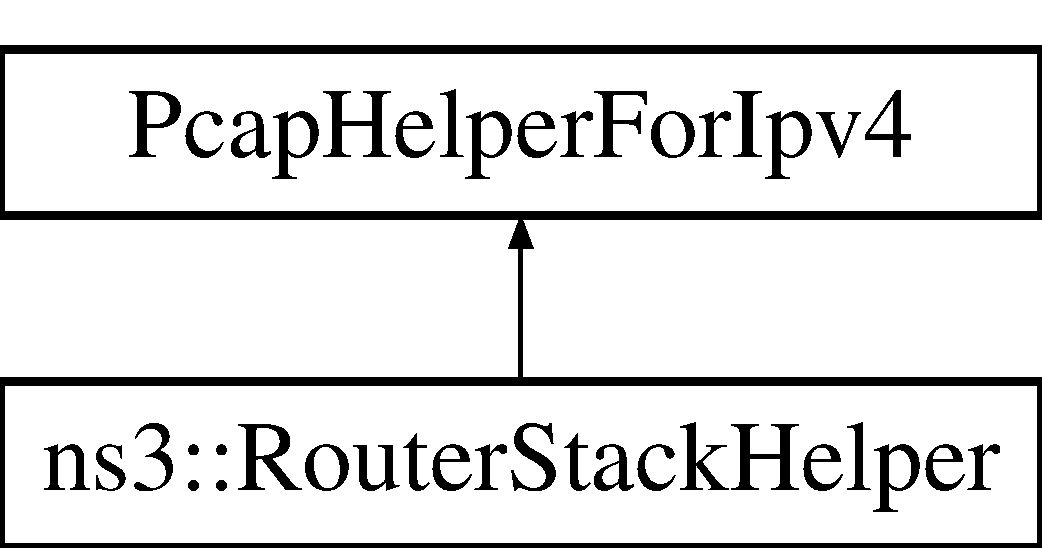
\includegraphics[height=2.000000cm]{classns3_1_1RouterStackHelper}
\end{center}
\end{figure}
\subsection*{Public Member Functions}
\begin{DoxyCompactItemize}
\item 
\hyperlink{classns3_1_1RouterStackHelper_afe2cc8f748caa13e72f9e2616b77c0e0}{Router\-Stack\-Helper} (void)
\item 
virtual \hyperlink{classns3_1_1RouterStackHelper_a3673fd8fb8184df5782b6e8538f6f1f6}{$\sim$\-Router\-Stack\-Helper} (void)
\item 
void \hyperlink{classns3_1_1RouterStackHelper_a0980b1c2c1fe1d05c40407558d06d649}{Reset} (void)
\item 
void \hyperlink{classns3_1_1RouterStackHelper_af322270b340c9f3b8df134d6e40671f3}{Set\-Routing\-Helper} (const Ipv4\-Routing\-Helper \&routing)
\item 
void \hyperlink{classns3_1_1RouterStackHelper_a94bdee66b5610184b317cdf107b27009}{Install} (std\-::string node\-Name) const 
\item 
void \hyperlink{classns3_1_1RouterStackHelper_a1fc5ba02a5cf54f0f008c15c4274531f}{Install} (Ptr$<$ Node $>$ node) const 
\item 
void \hyperlink{classns3_1_1RouterStackHelper_aa3d80267344ae81207ed2b5f1fab10bd}{Install} (Node\-Container c) const 
\item 
void \hyperlink{classns3_1_1RouterStackHelper_a46c4452fb80e27565675e69ee1a8f0f3}{Install\-All} (void) const 
\item 
void \hyperlink{classns3_1_1RouterStackHelper_a232b94c9750c49a70171b9aa3f9151b9}{Set\-Ipv4\-Stack\-Install} (bool enable)
\begin{DoxyCompactList}\small\item\em Enable/disable I\-Pv4 stack install. \end{DoxyCompactList}\item 
void \hyperlink{classns3_1_1RouterStackHelper_a33d51c290dae0395823847050645a38c}{Set\-Ipv4\-Arp\-Jitter} (bool enable)
\begin{DoxyCompactList}\small\item\em Enable/disable I\-Pv4 A\-R\-P Jitter. \end{DoxyCompactList}\item 
int64\-\_\-t \hyperlink{classns3_1_1RouterStackHelper_a150c650fa7384b68f6cc3b20e848b225}{Assign\-Streams} (Node\-Container c, int64\-\_\-t stream)
\item 
void \hyperlink{classns3_1_1RouterStackHelper_a957f8f558018bc7bfde76dc6047f64fd}{Set\-Cache\-Type} (std\-::string type\-Id)
\begin{DoxyCompactList}\small\item\em Get the Type\-Id of the subclass of \hyperlink{classns3_1_1NamedContentCache}{Named\-Content\-Cache}, that implements the required caching policy. \end{DoxyCompactList}\item 
std\-::string \hyperlink{classns3_1_1RouterStackHelper_a40b9a37ad83851c7949451589a422d16}{Get\-Cache\-Type} (void)
\begin{DoxyCompactList}\small\item\em Get the Type\-Id of the subclass of \hyperlink{classns3_1_1NamedContentCache}{Named\-Content\-Cache}, that implements the required caching policy. \end{DoxyCompactList}\item 
void \hyperlink{classns3_1_1RouterStackHelper_abad859db7b5bee7d1c4be9201a7972a8}{Set\-Cache\-Size} (uint32\-\_\-t size)
\begin{DoxyCompactList}\small\item\em Set the size of the cache of the I\-C\-N Router. \end{DoxyCompactList}\item 
void \hyperlink{classns3_1_1RouterStackHelper_a22e495a52aa107933c359eab17b8596f}{Control\-Cachability} (bool non\-\_\-cachable)
\begin{DoxyCompactList}\small\item\em Function to set content is cachable or not at I\-C\-N Router. \end{DoxyCompactList}\item 
void \hyperlink{classns3_1_1RouterStackHelper_a429a9b77f6b21301088125b4832a9cbf}{Set\-Freshness\-Time} (uint64\-\_\-t time)
\begin{DoxyCompactList}\small\item\em Set the freshness time for the contents of the cache of the I\-C\-N Router. \end{DoxyCompactList}\item 
uint64\-\_\-t \hyperlink{classns3_1_1RouterStackHelper_a6da6ab4e527893908dd351789230f03a}{Get\-Freshness\-Time} (void)
\begin{DoxyCompactList}\small\item\em Get the freshness time set for the contents of the cache of the I\-C\-N Router. \end{DoxyCompactList}\end{DoxyCompactItemize}
\subsection*{Private Member Functions}
\begin{DoxyCompactItemize}
\item 
virtual void \hyperlink{classns3_1_1RouterStackHelper_ac294402e8d59a7bdd294332cc4b3d33a}{Enable\-Pcap\-Ipv4\-Internal} (std\-::string prefix, Ptr$<$ Ipv4 $>$ ipv4, uint32\-\_\-t interface, bool explicit\-Filename)
\begin{DoxyCompactList}\small\item\em Enable pcap output the indicated Ipv4 and interface pair. \end{DoxyCompactList}\item 
void \hyperlink{classns3_1_1RouterStackHelper_abd09ae05773a9a706997514d4f807fcb}{Initialize} (void)
\begin{DoxyCompactList}\small\item\em Initialize the helper to its default values. \end{DoxyCompactList}\item 
bool \hyperlink{classns3_1_1RouterStackHelper_aabf5ed0df547a1ab881b9db4604966ca}{Pcap\-Hooked} (Ptr$<$ Ipv4 $>$ ipv4)
\end{DoxyCompactItemize}
\subsection*{Static Private Member Functions}
\begin{DoxyCompactItemize}
\item 
static void \hyperlink{classns3_1_1RouterStackHelper_a2b7ed097c3e34fa5efcd431bf541036e}{Create\-And\-Aggregate\-Object\-From\-Type\-Id} (Ptr$<$ Node $>$ node, std\-::string type\-Id)
\item 
static void \hyperlink{classns3_1_1RouterStackHelper_a216a05a70257f4c669e68b833e8ec6fb}{Create\-And\-Aggregate\-Object\-From\-Type\-Id} (Ptr$<$ Node $>$ node, std\-::string type\-Id, bool t)
\item 
static void \hyperlink{classns3_1_1RouterStackHelper_a6ddb140133a71f5347ecaca6f79ff969}{Cleanup} (void)
\end{DoxyCompactItemize}
\subsection*{Private Attributes}
\begin{DoxyCompactItemize}
\item 
const Ipv4\-Routing\-Helper $\ast$ \hyperlink{classns3_1_1RouterStackHelper_afce5b67df8aff1a4a8fca50a32d0d746}{m\-\_\-routing}
\item 
bool \hyperlink{classns3_1_1RouterStackHelper_a53fa9e728900f9fad07e49487b1b5131}{m\-\_\-ipv4\-Enabled}
\item 
bool \hyperlink{classns3_1_1RouterStackHelper_afb7a40b6e245447f3d9fd6e55afb9a6f}{m\-\_\-ipv4\-Arp\-Jitter\-Enabled}
\item 
std\-::string \hyperlink{classns3_1_1RouterStackHelper_a00676974faf0f9061cdfa64e2b2481f3}{cache\-\_\-type}
\begin{DoxyCompactList}\small\item\em Type\-Id of the sublclass of \hyperlink{classns3_1_1NamedContentCache}{Named\-Content\-Cache}. \end{DoxyCompactList}\item 
bool \hyperlink{classns3_1_1RouterStackHelper_a0c094073c949fe9d5bbe3ec66b2311e6}{m\-\_\-non\-\_\-cachable}
\item 
uint32\-\_\-t \hyperlink{classns3_1_1RouterStackHelper_af1bcf688f4db05e771f97c5cc3f151b9}{cache\-\_\-size}
\begin{DoxyCompactList}\small\item\em Cache size of the cache of I\-C\-N Router. \end{DoxyCompactList}\item 
uint64\-\_\-t \hyperlink{classns3_1_1RouterStackHelper_abde25db92b103214ca320f74a3fea16f}{freshness\-\_\-time}
\begin{DoxyCompactList}\small\item\em freshness time set for the contents of the cache of I\-C\-N Router \end{DoxyCompactList}\end{DoxyCompactItemize}


\subsection{Detailed Description}
Aggregate I\-P/\-T\-C\-P/\-U\-D\-P and Caching functionality to only I\-C\-N Routers in the Network. 

This class is exactly same as the Internet\-Stack\-Helper of \hyperlink{namespacens3}{ns3}. The only difference being that additional A\-P\-Is that enable caching facility at I\-C\-N Routers are also aggregated along with the regular internet stack. Also, unlike Internet\-Stack\-Helper, this class aggregates \hyperlink{classns3_1_1Ipv4RouterL3Protocol}{Ipv4\-Router\-L3\-Protocol} instead of Ipv4\-L3\-Protocol for implementation of the Ipv4 Protocol. This helper is used to aggregate the requisite stack only at I\-C\-N Router nodes in a network implementing O\-I\-C\-N Architecture, while other nodes use the regular Internet\-Stack\-Helper of \hyperlink{namespacens3}{ns3}. 

\subsection{Constructor \& Destructor Documentation}
\hypertarget{classns3_1_1RouterStackHelper_afe2cc8f748caa13e72f9e2616b77c0e0}{\index{ns3\-::\-Router\-Stack\-Helper@{ns3\-::\-Router\-Stack\-Helper}!Router\-Stack\-Helper@{Router\-Stack\-Helper}}
\index{Router\-Stack\-Helper@{Router\-Stack\-Helper}!ns3::RouterStackHelper@{ns3\-::\-Router\-Stack\-Helper}}
\subsubsection[{Router\-Stack\-Helper}]{\setlength{\rightskip}{0pt plus 5cm}ns3\-::\-Router\-Stack\-Helper\-::\-Router\-Stack\-Helper (
\begin{DoxyParamCaption}
\item[{void}]{}
\end{DoxyParamCaption}
)}}\label{classns3_1_1RouterStackHelper_afe2cc8f748caa13e72f9e2616b77c0e0}
Create a new \hyperlink{classns3_1_1RouterStackHelper}{Router\-Stack\-Helper} which uses a mix of static routing and global routing by default. The static routing protocol (ns3\-::\-Ipv4\-Static\-Routing) and the global routing protocol are stored in an ns3\-::\-Ipv4\-List\-Routing protocol with priorities 0, and -\/10 by default. If you wish to use different priorites and different routing protocols, you need to use an adhoc ns3\-::\-Ipv4\-Routing\-Helper, such as ns3\-::\-Olsr\-Helper \hypertarget{classns3_1_1RouterStackHelper_a3673fd8fb8184df5782b6e8538f6f1f6}{\index{ns3\-::\-Router\-Stack\-Helper@{ns3\-::\-Router\-Stack\-Helper}!$\sim$\-Router\-Stack\-Helper@{$\sim$\-Router\-Stack\-Helper}}
\index{$\sim$\-Router\-Stack\-Helper@{$\sim$\-Router\-Stack\-Helper}!ns3::RouterStackHelper@{ns3\-::\-Router\-Stack\-Helper}}
\subsubsection[{$\sim$\-Router\-Stack\-Helper}]{\setlength{\rightskip}{0pt plus 5cm}ns3\-::\-Router\-Stack\-Helper\-::$\sim$\-Router\-Stack\-Helper (
\begin{DoxyParamCaption}
\item[{void}]{}
\end{DoxyParamCaption}
)\hspace{0.3cm}{\ttfamily [virtual]}}}\label{classns3_1_1RouterStackHelper_a3673fd8fb8184df5782b6e8538f6f1f6}
Destroy the \hyperlink{classns3_1_1RouterStackHelper}{Router\-Stack\-Helper} 

\subsection{Member Function Documentation}
\hypertarget{classns3_1_1RouterStackHelper_a150c650fa7384b68f6cc3b20e848b225}{\index{ns3\-::\-Router\-Stack\-Helper@{ns3\-::\-Router\-Stack\-Helper}!Assign\-Streams@{Assign\-Streams}}
\index{Assign\-Streams@{Assign\-Streams}!ns3::RouterStackHelper@{ns3\-::\-Router\-Stack\-Helper}}
\subsubsection[{Assign\-Streams}]{\setlength{\rightskip}{0pt plus 5cm}int64\-\_\-t ns3\-::\-Router\-Stack\-Helper\-::\-Assign\-Streams (
\begin{DoxyParamCaption}
\item[{Node\-Container}]{c, }
\item[{int64\-\_\-t}]{stream}
\end{DoxyParamCaption}
)}}\label{classns3_1_1RouterStackHelper_a150c650fa7384b68f6cc3b20e848b225}
Assign a fixed random variable stream number to the random variables used by this model. Return the number of streams (possibly zero) that have been assigned. The \hyperlink{classns3_1_1RouterStackHelper_a94bdee66b5610184b317cdf107b27009}{Install()} method should have previously been called by the user.


\begin{DoxyParams}{Parameters}
{\em stream} & first stream index to use \\
\hline
{\em c} & Node\-Container of the set of nodes for which the internet models should be modified to use a fixed stream \\
\hline
\end{DoxyParams}
\begin{DoxyReturn}{Returns}
the number of stream indices assigned by this helper 
\end{DoxyReturn}
\hypertarget{classns3_1_1RouterStackHelper_a6ddb140133a71f5347ecaca6f79ff969}{\index{ns3\-::\-Router\-Stack\-Helper@{ns3\-::\-Router\-Stack\-Helper}!Cleanup@{Cleanup}}
\index{Cleanup@{Cleanup}!ns3::RouterStackHelper@{ns3\-::\-Router\-Stack\-Helper}}
\subsubsection[{Cleanup}]{\setlength{\rightskip}{0pt plus 5cm}static void ns3\-::\-Router\-Stack\-Helper\-::\-Cleanup (
\begin{DoxyParamCaption}
\item[{void}]{}
\end{DoxyParamCaption}
)\hspace{0.3cm}{\ttfamily [static]}, {\ttfamily [private]}}}\label{classns3_1_1RouterStackHelper_a6ddb140133a71f5347ecaca6f79ff969}
\hypertarget{classns3_1_1RouterStackHelper_a22e495a52aa107933c359eab17b8596f}{\index{ns3\-::\-Router\-Stack\-Helper@{ns3\-::\-Router\-Stack\-Helper}!Control\-Cachability@{Control\-Cachability}}
\index{Control\-Cachability@{Control\-Cachability}!ns3::RouterStackHelper@{ns3\-::\-Router\-Stack\-Helper}}
\subsubsection[{Control\-Cachability}]{\setlength{\rightskip}{0pt plus 5cm}void ns3\-::\-Router\-Stack\-Helper\-::\-Control\-Cachability (
\begin{DoxyParamCaption}
\item[{bool}]{non\-\_\-cachable}
\end{DoxyParamCaption}
)}}\label{classns3_1_1RouterStackHelper_a22e495a52aa107933c359eab17b8596f}


Function to set content is cachable or not at I\-C\-N Router. 


\begin{DoxyParams}{Parameters}
{\em non\-\_\-cachable} & parameter to set cacheability of the content, if true then non-\/cacheable otherwise cacheable \\
\hline
\end{DoxyParams}
\hypertarget{classns3_1_1RouterStackHelper_a2b7ed097c3e34fa5efcd431bf541036e}{\index{ns3\-::\-Router\-Stack\-Helper@{ns3\-::\-Router\-Stack\-Helper}!Create\-And\-Aggregate\-Object\-From\-Type\-Id@{Create\-And\-Aggregate\-Object\-From\-Type\-Id}}
\index{Create\-And\-Aggregate\-Object\-From\-Type\-Id@{Create\-And\-Aggregate\-Object\-From\-Type\-Id}!ns3::RouterStackHelper@{ns3\-::\-Router\-Stack\-Helper}}
\subsubsection[{Create\-And\-Aggregate\-Object\-From\-Type\-Id}]{\setlength{\rightskip}{0pt plus 5cm}void ns3\-::\-Router\-Stack\-Helper\-::\-Create\-And\-Aggregate\-Object\-From\-Type\-Id (
\begin{DoxyParamCaption}
\item[{Ptr$<$ Node $>$}]{node, }
\item[{std\-::string}]{type\-Id}
\end{DoxyParamCaption}
)\hspace{0.3cm}{\ttfamily [static]}, {\ttfamily [private]}}}\label{classns3_1_1RouterStackHelper_a2b7ed097c3e34fa5efcd431bf541036e}
\hypertarget{classns3_1_1RouterStackHelper_a216a05a70257f4c669e68b833e8ec6fb}{\index{ns3\-::\-Router\-Stack\-Helper@{ns3\-::\-Router\-Stack\-Helper}!Create\-And\-Aggregate\-Object\-From\-Type\-Id@{Create\-And\-Aggregate\-Object\-From\-Type\-Id}}
\index{Create\-And\-Aggregate\-Object\-From\-Type\-Id@{Create\-And\-Aggregate\-Object\-From\-Type\-Id}!ns3::RouterStackHelper@{ns3\-::\-Router\-Stack\-Helper}}
\subsubsection[{Create\-And\-Aggregate\-Object\-From\-Type\-Id}]{\setlength{\rightskip}{0pt plus 5cm}void ns3\-::\-Router\-Stack\-Helper\-::\-Create\-And\-Aggregate\-Object\-From\-Type\-Id (
\begin{DoxyParamCaption}
\item[{Ptr$<$ Node $>$}]{node, }
\item[{std\-::string}]{type\-Id, }
\item[{bool}]{t}
\end{DoxyParamCaption}
)\hspace{0.3cm}{\ttfamily [static]}, {\ttfamily [private]}}}\label{classns3_1_1RouterStackHelper_a216a05a70257f4c669e68b833e8ec6fb}
\hypertarget{classns3_1_1RouterStackHelper_ac294402e8d59a7bdd294332cc4b3d33a}{\index{ns3\-::\-Router\-Stack\-Helper@{ns3\-::\-Router\-Stack\-Helper}!Enable\-Pcap\-Ipv4\-Internal@{Enable\-Pcap\-Ipv4\-Internal}}
\index{Enable\-Pcap\-Ipv4\-Internal@{Enable\-Pcap\-Ipv4\-Internal}!ns3::RouterStackHelper@{ns3\-::\-Router\-Stack\-Helper}}
\subsubsection[{Enable\-Pcap\-Ipv4\-Internal}]{\setlength{\rightskip}{0pt plus 5cm}void ns3\-::\-Router\-Stack\-Helper\-::\-Enable\-Pcap\-Ipv4\-Internal (
\begin{DoxyParamCaption}
\item[{std\-::string}]{prefix, }
\item[{Ptr$<$ Ipv4 $>$}]{ipv4, }
\item[{uint32\-\_\-t}]{interface, }
\item[{bool}]{explicit\-Filename}
\end{DoxyParamCaption}
)\hspace{0.3cm}{\ttfamily [private]}, {\ttfamily [virtual]}}}\label{classns3_1_1RouterStackHelper_ac294402e8d59a7bdd294332cc4b3d33a}


Enable pcap output the indicated Ipv4 and interface pair. 

\hypertarget{classns3_1_1RouterStackHelper_a40b9a37ad83851c7949451589a422d16}{\index{ns3\-::\-Router\-Stack\-Helper@{ns3\-::\-Router\-Stack\-Helper}!Get\-Cache\-Type@{Get\-Cache\-Type}}
\index{Get\-Cache\-Type@{Get\-Cache\-Type}!ns3::RouterStackHelper@{ns3\-::\-Router\-Stack\-Helper}}
\subsubsection[{Get\-Cache\-Type}]{\setlength{\rightskip}{0pt plus 5cm}std\-::string ns3\-::\-Router\-Stack\-Helper\-::\-Get\-Cache\-Type (
\begin{DoxyParamCaption}
\item[{void}]{}
\end{DoxyParamCaption}
)}}\label{classns3_1_1RouterStackHelper_a40b9a37ad83851c7949451589a422d16}


Get the Type\-Id of the subclass of \hyperlink{classns3_1_1NamedContentCache}{Named\-Content\-Cache}, that implements the required caching policy. 

\begin{DoxyReturn}{Returns}
the Type\-Id of the subclass 
\end{DoxyReturn}
\hypertarget{classns3_1_1RouterStackHelper_a6da6ab4e527893908dd351789230f03a}{\index{ns3\-::\-Router\-Stack\-Helper@{ns3\-::\-Router\-Stack\-Helper}!Get\-Freshness\-Time@{Get\-Freshness\-Time}}
\index{Get\-Freshness\-Time@{Get\-Freshness\-Time}!ns3::RouterStackHelper@{ns3\-::\-Router\-Stack\-Helper}}
\subsubsection[{Get\-Freshness\-Time}]{\setlength{\rightskip}{0pt plus 5cm}uint64\-\_\-t ns3\-::\-Router\-Stack\-Helper\-::\-Get\-Freshness\-Time (
\begin{DoxyParamCaption}
\item[{void}]{}
\end{DoxyParamCaption}
)}}\label{classns3_1_1RouterStackHelper_a6da6ab4e527893908dd351789230f03a}


Get the freshness time set for the contents of the cache of the I\-C\-N Router. 

\begin{DoxyReturn}{Returns}
the freshness time 
\end{DoxyReturn}
\hypertarget{classns3_1_1RouterStackHelper_abd09ae05773a9a706997514d4f807fcb}{\index{ns3\-::\-Router\-Stack\-Helper@{ns3\-::\-Router\-Stack\-Helper}!Initialize@{Initialize}}
\index{Initialize@{Initialize}!ns3::RouterStackHelper@{ns3\-::\-Router\-Stack\-Helper}}
\subsubsection[{Initialize}]{\setlength{\rightskip}{0pt plus 5cm}void ns3\-::\-Router\-Stack\-Helper\-::\-Initialize (
\begin{DoxyParamCaption}
\item[{void}]{}
\end{DoxyParamCaption}
)\hspace{0.3cm}{\ttfamily [private]}}}\label{classns3_1_1RouterStackHelper_abd09ae05773a9a706997514d4f807fcb}


Initialize the helper to its default values. 

\hypertarget{classns3_1_1RouterStackHelper_a94bdee66b5610184b317cdf107b27009}{\index{ns3\-::\-Router\-Stack\-Helper@{ns3\-::\-Router\-Stack\-Helper}!Install@{Install}}
\index{Install@{Install}!ns3::RouterStackHelper@{ns3\-::\-Router\-Stack\-Helper}}
\subsubsection[{Install}]{\setlength{\rightskip}{0pt plus 5cm}void ns3\-::\-Router\-Stack\-Helper\-::\-Install (
\begin{DoxyParamCaption}
\item[{std\-::string}]{node\-Name}
\end{DoxyParamCaption}
) const}}\label{classns3_1_1RouterStackHelper_a94bdee66b5610184b317cdf107b27009}
Aggregate implementations of the ns3\-::\-Ipv4, ns3\-::\-Udp, and ns3\-::\-Tcp classes onto the provided node. This method will assert if called on a node that already has an Ipv4 object aggregated to it.


\begin{DoxyParams}{Parameters}
{\em node\-Name} & The name of the node on which to install the stack. \\
\hline
\end{DoxyParams}
\hypertarget{classns3_1_1RouterStackHelper_a1fc5ba02a5cf54f0f008c15c4274531f}{\index{ns3\-::\-Router\-Stack\-Helper@{ns3\-::\-Router\-Stack\-Helper}!Install@{Install}}
\index{Install@{Install}!ns3::RouterStackHelper@{ns3\-::\-Router\-Stack\-Helper}}
\subsubsection[{Install}]{\setlength{\rightskip}{0pt plus 5cm}void ns3\-::\-Router\-Stack\-Helper\-::\-Install (
\begin{DoxyParamCaption}
\item[{Ptr$<$ Node $>$}]{node}
\end{DoxyParamCaption}
) const}}\label{classns3_1_1RouterStackHelper_a1fc5ba02a5cf54f0f008c15c4274531f}
Aggregate implementations of the ns3\-::\-Ipv4, ns3\-::\-Udp, and ns3\-::\-Tcp classes onto the provided node. Also aggregate classes that implement caching functionalities. This method will assert if called on a node that already has an Ipv4 object aggregated to it.


\begin{DoxyParams}{Parameters}
{\em node} & The node on which to install the stack. \\
\hline
\end{DoxyParams}
\hypertarget{classns3_1_1RouterStackHelper_aa3d80267344ae81207ed2b5f1fab10bd}{\index{ns3\-::\-Router\-Stack\-Helper@{ns3\-::\-Router\-Stack\-Helper}!Install@{Install}}
\index{Install@{Install}!ns3::RouterStackHelper@{ns3\-::\-Router\-Stack\-Helper}}
\subsubsection[{Install}]{\setlength{\rightskip}{0pt plus 5cm}void ns3\-::\-Router\-Stack\-Helper\-::\-Install (
\begin{DoxyParamCaption}
\item[{Node\-Container}]{c}
\end{DoxyParamCaption}
) const}}\label{classns3_1_1RouterStackHelper_aa3d80267344ae81207ed2b5f1fab10bd}
For each node in the input container, aggregate implementations of the ns3\-::\-Ipv4, ns3\-::\-Udp, and, ns3\-::\-Tcp classes. The program will assert if this method is called on a container with a node that already has an Ipv4 object aggregated to it.


\begin{DoxyParams}{Parameters}
{\em c} & Node\-Container that holds the set of nodes on which to install the new stacks. \\
\hline
\end{DoxyParams}
\hypertarget{classns3_1_1RouterStackHelper_a46c4452fb80e27565675e69ee1a8f0f3}{\index{ns3\-::\-Router\-Stack\-Helper@{ns3\-::\-Router\-Stack\-Helper}!Install\-All@{Install\-All}}
\index{Install\-All@{Install\-All}!ns3::RouterStackHelper@{ns3\-::\-Router\-Stack\-Helper}}
\subsubsection[{Install\-All}]{\setlength{\rightskip}{0pt plus 5cm}void ns3\-::\-Router\-Stack\-Helper\-::\-Install\-All (
\begin{DoxyParamCaption}
\item[{void}]{}
\end{DoxyParamCaption}
) const}}\label{classns3_1_1RouterStackHelper_a46c4452fb80e27565675e69ee1a8f0f3}
Aggregate I\-Pv4, I\-Pv6, U\-D\-P, and T\-C\-P stacks to all nodes in the simulation \hypertarget{classns3_1_1RouterStackHelper_aabf5ed0df547a1ab881b9db4604966ca}{\index{ns3\-::\-Router\-Stack\-Helper@{ns3\-::\-Router\-Stack\-Helper}!Pcap\-Hooked@{Pcap\-Hooked}}
\index{Pcap\-Hooked@{Pcap\-Hooked}!ns3::RouterStackHelper@{ns3\-::\-Router\-Stack\-Helper}}
\subsubsection[{Pcap\-Hooked}]{\setlength{\rightskip}{0pt plus 5cm}bool ns3\-::\-Router\-Stack\-Helper\-::\-Pcap\-Hooked (
\begin{DoxyParamCaption}
\item[{Ptr$<$ Ipv4 $>$}]{ipv4}
\end{DoxyParamCaption}
)\hspace{0.3cm}{\ttfamily [private]}}}\label{classns3_1_1RouterStackHelper_aabf5ed0df547a1ab881b9db4604966ca}
\hypertarget{classns3_1_1RouterStackHelper_a0980b1c2c1fe1d05c40407558d06d649}{\index{ns3\-::\-Router\-Stack\-Helper@{ns3\-::\-Router\-Stack\-Helper}!Reset@{Reset}}
\index{Reset@{Reset}!ns3::RouterStackHelper@{ns3\-::\-Router\-Stack\-Helper}}
\subsubsection[{Reset}]{\setlength{\rightskip}{0pt plus 5cm}void ns3\-::\-Router\-Stack\-Helper\-::\-Reset (
\begin{DoxyParamCaption}
\item[{void}]{}
\end{DoxyParamCaption}
)}}\label{classns3_1_1RouterStackHelper_a0980b1c2c1fe1d05c40407558d06d649}
Return helper internal state to that of a newly constructed one \hypertarget{classns3_1_1RouterStackHelper_abad859db7b5bee7d1c4be9201a7972a8}{\index{ns3\-::\-Router\-Stack\-Helper@{ns3\-::\-Router\-Stack\-Helper}!Set\-Cache\-Size@{Set\-Cache\-Size}}
\index{Set\-Cache\-Size@{Set\-Cache\-Size}!ns3::RouterStackHelper@{ns3\-::\-Router\-Stack\-Helper}}
\subsubsection[{Set\-Cache\-Size}]{\setlength{\rightskip}{0pt plus 5cm}void ns3\-::\-Router\-Stack\-Helper\-::\-Set\-Cache\-Size (
\begin{DoxyParamCaption}
\item[{uint32\-\_\-t}]{size}
\end{DoxyParamCaption}
)}}\label{classns3_1_1RouterStackHelper_abad859db7b5bee7d1c4be9201a7972a8}


Set the size of the cache of the I\-C\-N Router. 


\begin{DoxyParams}{Parameters}
{\em size} & cache size to be set \\
\hline
\end{DoxyParams}
\hypertarget{classns3_1_1RouterStackHelper_a957f8f558018bc7bfde76dc6047f64fd}{\index{ns3\-::\-Router\-Stack\-Helper@{ns3\-::\-Router\-Stack\-Helper}!Set\-Cache\-Type@{Set\-Cache\-Type}}
\index{Set\-Cache\-Type@{Set\-Cache\-Type}!ns3::RouterStackHelper@{ns3\-::\-Router\-Stack\-Helper}}
\subsubsection[{Set\-Cache\-Type}]{\setlength{\rightskip}{0pt plus 5cm}void ns3\-::\-Router\-Stack\-Helper\-::\-Set\-Cache\-Type (
\begin{DoxyParamCaption}
\item[{std\-::string}]{type\-Id}
\end{DoxyParamCaption}
)}}\label{classns3_1_1RouterStackHelper_a957f8f558018bc7bfde76dc6047f64fd}


Get the Type\-Id of the subclass of \hyperlink{classns3_1_1NamedContentCache}{Named\-Content\-Cache}, that implements the required caching policy. 

\begin{DoxyReturn}{Returns}
the Type\-Id of the subclass 
\end{DoxyReturn}
\hypertarget{classns3_1_1RouterStackHelper_a429a9b77f6b21301088125b4832a9cbf}{\index{ns3\-::\-Router\-Stack\-Helper@{ns3\-::\-Router\-Stack\-Helper}!Set\-Freshness\-Time@{Set\-Freshness\-Time}}
\index{Set\-Freshness\-Time@{Set\-Freshness\-Time}!ns3::RouterStackHelper@{ns3\-::\-Router\-Stack\-Helper}}
\subsubsection[{Set\-Freshness\-Time}]{\setlength{\rightskip}{0pt plus 5cm}void ns3\-::\-Router\-Stack\-Helper\-::\-Set\-Freshness\-Time (
\begin{DoxyParamCaption}
\item[{uint64\-\_\-t}]{time}
\end{DoxyParamCaption}
)}}\label{classns3_1_1RouterStackHelper_a429a9b77f6b21301088125b4832a9cbf}


Set the freshness time for the contents of the cache of the I\-C\-N Router. 


\begin{DoxyParams}{Parameters}
{\em time} & freshness time to be set \\
\hline
\end{DoxyParams}
\hypertarget{classns3_1_1RouterStackHelper_a33d51c290dae0395823847050645a38c}{\index{ns3\-::\-Router\-Stack\-Helper@{ns3\-::\-Router\-Stack\-Helper}!Set\-Ipv4\-Arp\-Jitter@{Set\-Ipv4\-Arp\-Jitter}}
\index{Set\-Ipv4\-Arp\-Jitter@{Set\-Ipv4\-Arp\-Jitter}!ns3::RouterStackHelper@{ns3\-::\-Router\-Stack\-Helper}}
\subsubsection[{Set\-Ipv4\-Arp\-Jitter}]{\setlength{\rightskip}{0pt plus 5cm}void ns3\-::\-Router\-Stack\-Helper\-::\-Set\-Ipv4\-Arp\-Jitter (
\begin{DoxyParamCaption}
\item[{bool}]{enable}
\end{DoxyParamCaption}
)}}\label{classns3_1_1RouterStackHelper_a33d51c290dae0395823847050645a38c}


Enable/disable I\-Pv4 A\-R\-P Jitter. 


\begin{DoxyParams}{Parameters}
{\em enable} & enable state \\
\hline
\end{DoxyParams}
\hypertarget{classns3_1_1RouterStackHelper_a232b94c9750c49a70171b9aa3f9151b9}{\index{ns3\-::\-Router\-Stack\-Helper@{ns3\-::\-Router\-Stack\-Helper}!Set\-Ipv4\-Stack\-Install@{Set\-Ipv4\-Stack\-Install}}
\index{Set\-Ipv4\-Stack\-Install@{Set\-Ipv4\-Stack\-Install}!ns3::RouterStackHelper@{ns3\-::\-Router\-Stack\-Helper}}
\subsubsection[{Set\-Ipv4\-Stack\-Install}]{\setlength{\rightskip}{0pt plus 5cm}void ns3\-::\-Router\-Stack\-Helper\-::\-Set\-Ipv4\-Stack\-Install (
\begin{DoxyParamCaption}
\item[{bool}]{enable}
\end{DoxyParamCaption}
)}}\label{classns3_1_1RouterStackHelper_a232b94c9750c49a70171b9aa3f9151b9}


Enable/disable I\-Pv4 stack install. 


\begin{DoxyParams}{Parameters}
{\em enable} & enable state \\
\hline
\end{DoxyParams}
\hypertarget{classns3_1_1RouterStackHelper_af322270b340c9f3b8df134d6e40671f3}{\index{ns3\-::\-Router\-Stack\-Helper@{ns3\-::\-Router\-Stack\-Helper}!Set\-Routing\-Helper@{Set\-Routing\-Helper}}
\index{Set\-Routing\-Helper@{Set\-Routing\-Helper}!ns3::RouterStackHelper@{ns3\-::\-Router\-Stack\-Helper}}
\subsubsection[{Set\-Routing\-Helper}]{\setlength{\rightskip}{0pt plus 5cm}void ns3\-::\-Router\-Stack\-Helper\-::\-Set\-Routing\-Helper (
\begin{DoxyParamCaption}
\item[{const Ipv4\-Routing\-Helper \&}]{routing}
\end{DoxyParamCaption}
)}}\label{classns3_1_1RouterStackHelper_af322270b340c9f3b8df134d6e40671f3}

\begin{DoxyParams}{Parameters}
{\em routing} & a new routing helper\\
\hline
\end{DoxyParams}
Set the routing helper to use during Install. The routing helper is really an object factory which is used to create an object of type ns3\-::\-Ipv4\-Routing\-Protocol per node. This routing object is then associated to a single ns3\-::\-Ipv4 object through its ns3\-::\-Ipv4\-::\-Set\-Routing\-Protocol. 

\subsection{Member Data Documentation}
\hypertarget{classns3_1_1RouterStackHelper_af1bcf688f4db05e771f97c5cc3f151b9}{\index{ns3\-::\-Router\-Stack\-Helper@{ns3\-::\-Router\-Stack\-Helper}!cache\-\_\-size@{cache\-\_\-size}}
\index{cache\-\_\-size@{cache\-\_\-size}!ns3::RouterStackHelper@{ns3\-::\-Router\-Stack\-Helper}}
\subsubsection[{cache\-\_\-size}]{\setlength{\rightskip}{0pt plus 5cm}uint32\-\_\-t ns3\-::\-Router\-Stack\-Helper\-::cache\-\_\-size\hspace{0.3cm}{\ttfamily [private]}}}\label{classns3_1_1RouterStackHelper_af1bcf688f4db05e771f97c5cc3f151b9}


Cache size of the cache of I\-C\-N Router. 

\hypertarget{classns3_1_1RouterStackHelper_a00676974faf0f9061cdfa64e2b2481f3}{\index{ns3\-::\-Router\-Stack\-Helper@{ns3\-::\-Router\-Stack\-Helper}!cache\-\_\-type@{cache\-\_\-type}}
\index{cache\-\_\-type@{cache\-\_\-type}!ns3::RouterStackHelper@{ns3\-::\-Router\-Stack\-Helper}}
\subsubsection[{cache\-\_\-type}]{\setlength{\rightskip}{0pt plus 5cm}std\-::string ns3\-::\-Router\-Stack\-Helper\-::cache\-\_\-type\hspace{0.3cm}{\ttfamily [private]}}}\label{classns3_1_1RouterStackHelper_a00676974faf0f9061cdfa64e2b2481f3}


Type\-Id of the sublclass of \hyperlink{classns3_1_1NamedContentCache}{Named\-Content\-Cache}. 

\hypertarget{classns3_1_1RouterStackHelper_abde25db92b103214ca320f74a3fea16f}{\index{ns3\-::\-Router\-Stack\-Helper@{ns3\-::\-Router\-Stack\-Helper}!freshness\-\_\-time@{freshness\-\_\-time}}
\index{freshness\-\_\-time@{freshness\-\_\-time}!ns3::RouterStackHelper@{ns3\-::\-Router\-Stack\-Helper}}
\subsubsection[{freshness\-\_\-time}]{\setlength{\rightskip}{0pt plus 5cm}uint64\-\_\-t ns3\-::\-Router\-Stack\-Helper\-::freshness\-\_\-time\hspace{0.3cm}{\ttfamily [private]}}}\label{classns3_1_1RouterStackHelper_abde25db92b103214ca320f74a3fea16f}


freshness time set for the contents of the cache of I\-C\-N Router 

\hypertarget{classns3_1_1RouterStackHelper_afb7a40b6e245447f3d9fd6e55afb9a6f}{\index{ns3\-::\-Router\-Stack\-Helper@{ns3\-::\-Router\-Stack\-Helper}!m\-\_\-ipv4\-Arp\-Jitter\-Enabled@{m\-\_\-ipv4\-Arp\-Jitter\-Enabled}}
\index{m\-\_\-ipv4\-Arp\-Jitter\-Enabled@{m\-\_\-ipv4\-Arp\-Jitter\-Enabled}!ns3::RouterStackHelper@{ns3\-::\-Router\-Stack\-Helper}}
\subsubsection[{m\-\_\-ipv4\-Arp\-Jitter\-Enabled}]{\setlength{\rightskip}{0pt plus 5cm}bool ns3\-::\-Router\-Stack\-Helper\-::m\-\_\-ipv4\-Arp\-Jitter\-Enabled\hspace{0.3cm}{\ttfamily [private]}}}\label{classns3_1_1RouterStackHelper_afb7a40b6e245447f3d9fd6e55afb9a6f}
\hypertarget{classns3_1_1RouterStackHelper_a53fa9e728900f9fad07e49487b1b5131}{\index{ns3\-::\-Router\-Stack\-Helper@{ns3\-::\-Router\-Stack\-Helper}!m\-\_\-ipv4\-Enabled@{m\-\_\-ipv4\-Enabled}}
\index{m\-\_\-ipv4\-Enabled@{m\-\_\-ipv4\-Enabled}!ns3::RouterStackHelper@{ns3\-::\-Router\-Stack\-Helper}}
\subsubsection[{m\-\_\-ipv4\-Enabled}]{\setlength{\rightskip}{0pt plus 5cm}bool ns3\-::\-Router\-Stack\-Helper\-::m\-\_\-ipv4\-Enabled\hspace{0.3cm}{\ttfamily [private]}}}\label{classns3_1_1RouterStackHelper_a53fa9e728900f9fad07e49487b1b5131}
\hypertarget{classns3_1_1RouterStackHelper_a0c094073c949fe9d5bbe3ec66b2311e6}{\index{ns3\-::\-Router\-Stack\-Helper@{ns3\-::\-Router\-Stack\-Helper}!m\-\_\-non\-\_\-cachable@{m\-\_\-non\-\_\-cachable}}
\index{m\-\_\-non\-\_\-cachable@{m\-\_\-non\-\_\-cachable}!ns3::RouterStackHelper@{ns3\-::\-Router\-Stack\-Helper}}
\subsubsection[{m\-\_\-non\-\_\-cachable}]{\setlength{\rightskip}{0pt plus 5cm}bool ns3\-::\-Router\-Stack\-Helper\-::m\-\_\-non\-\_\-cachable\hspace{0.3cm}{\ttfamily [private]}}}\label{classns3_1_1RouterStackHelper_a0c094073c949fe9d5bbe3ec66b2311e6}
\hypertarget{classns3_1_1RouterStackHelper_afce5b67df8aff1a4a8fca50a32d0d746}{\index{ns3\-::\-Router\-Stack\-Helper@{ns3\-::\-Router\-Stack\-Helper}!m\-\_\-routing@{m\-\_\-routing}}
\index{m\-\_\-routing@{m\-\_\-routing}!ns3::RouterStackHelper@{ns3\-::\-Router\-Stack\-Helper}}
\subsubsection[{m\-\_\-routing}]{\setlength{\rightskip}{0pt plus 5cm}const Ipv4\-Routing\-Helper$\ast$ ns3\-::\-Router\-Stack\-Helper\-::m\-\_\-routing\hspace{0.3cm}{\ttfamily [private]}}}\label{classns3_1_1RouterStackHelper_afce5b67df8aff1a4a8fca50a32d0d746}


The documentation for this class was generated from the following files\-:\begin{DoxyCompactItemize}
\item 
helper/\hyperlink{router-stack-helper_8h}{router-\/stack-\/helper.\-h}\item 
helper/\hyperlink{router-stack-helper_8cc}{router-\/stack-\/helper.\-cc}\end{DoxyCompactItemize}

\hypertarget{classns3_1_1SimpleUniversalCaching}{\section{ns3\-:\-:Simple\-Universal\-Caching Class Reference}
\label{classns3_1_1SimpleUniversalCaching}\index{ns3\-::\-Simple\-Universal\-Caching@{ns3\-::\-Simple\-Universal\-Caching}}
}


This class implements the Universal caching policy.  




{\ttfamily \#include $<$simple-\/universal-\/caching.\-h$>$}

Inheritance diagram for ns3\-:\-:Simple\-Universal\-Caching\-:\begin{figure}[H]
\begin{center}
\leavevmode
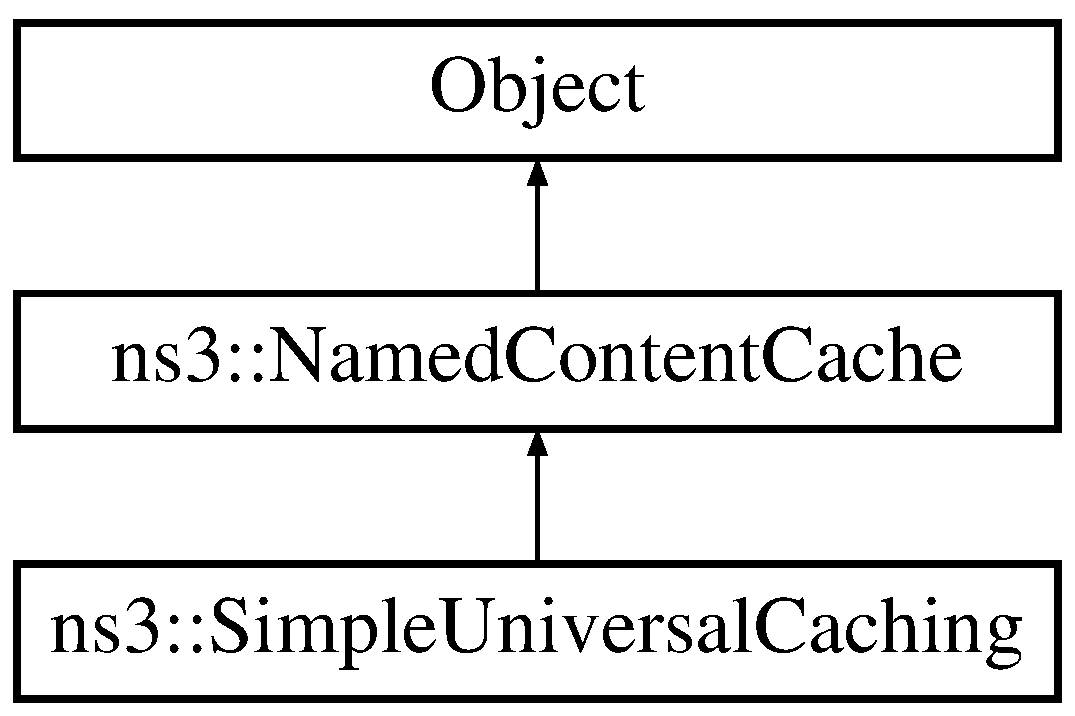
\includegraphics[height=3.000000cm]{classns3_1_1SimpleUniversalCaching}
\end{center}
\end{figure}
\subsection*{Public Member Functions}
\begin{DoxyCompactItemize}
\item 
\hyperlink{classns3_1_1SimpleUniversalCaching_a818bfd8d8077eef52cc33156373e00b5}{Simple\-Universal\-Caching} ()
\item 
virtual \hyperlink{classns3_1_1SimpleUniversalCaching_ac7a548d505befd6a65108bc043ab0715}{$\sim$\-Simple\-Universal\-Caching} ()
\item 
virtual void \hyperlink{classns3_1_1SimpleUniversalCaching_aa6123b2df8e357e30b84edf190d874c8}{Set\-Cache\-Size} (uint32\-\_\-t size)
\begin{DoxyCompactList}\small\item\em Set the cache size of the Cache. \end{DoxyCompactList}\item 
virtual uint32\-\_\-t \hyperlink{classns3_1_1SimpleUniversalCaching_a923d1d730c8d0171e2366773b950d165}{Get\-Cache\-Size} (void)
\begin{DoxyCompactList}\small\item\em Get the cache size of the Cache. \end{DoxyCompactList}\item 
virtual void \hyperlink{classns3_1_1SimpleUniversalCaching_a356fd57c44d67a96db68c5dbd0d8471c}{Set\-Freshness\-Time} (uint64\-\_\-t time)
\begin{DoxyCompactList}\small\item\em Set the freshness time for the contents of Cache. \end{DoxyCompactList}\item 
virtual uint64\-\_\-t \hyperlink{classns3_1_1SimpleUniversalCaching_a164cda8301046d0123443419528c6b3e}{Get\-Freshness\-Time} (void)
\begin{DoxyCompactList}\small\item\em Get the freshness time set for the contents of Cache. \end{DoxyCompactList}\item 
virtual \hyperlink{classns3_1_1NamedContentCacheEntry}{Named\-Content\-Cache\-Entry} \hyperlink{classns3_1_1SimpleUniversalCaching_a95d289d9580f5af31885b8deb9738451}{Create\-Entry} (std\-::string Name, Ptr$<$ Packet $>$ packet, Ipv4\-Header ipheader)
\begin{DoxyCompactList}\small\item\em Create the Cache entry, which is an object of \hyperlink{classns3_1_1NamedContentCacheEntry}{Named\-Content\-Cache\-Entry} class. The subclasses will define this function to create an entry that has the requisite parameters of the content, for the purpose of indexing content according to caching policy the subclass represents. \end{DoxyCompactList}\item 
virtual uint32\-\_\-t \hyperlink{classns3_1_1SimpleUniversalCaching_aeec1f45196ce8ffe82baf2439e4ee064}{Create\-Index} (\hyperlink{classns3_1_1NamedContentCacheEntry}{Named\-Content\-Cache\-Entry} entry)
\begin{DoxyCompactList}\small\item\em Create the index of the corresponding entry, by using the parameters of the content present in the entry class. The subclasses will define this function to create an index which, when put in order, will arrange the contents according to the caching policy the subclass represents. If some subclasses need decimal indexes, they have to multiply the obtained index with a factor to ensure unique integer indexes are obtained. \end{DoxyCompactList}\item 
virtual void \hyperlink{classns3_1_1SimpleUniversalCaching_a18713ba18ecbf1ef06b0efdf2ef3d83b}{Insert\-To\-Cache} (std\-::string Name, \hyperlink{classns3_1_1NamedContentCacheEntry}{Named\-Content\-Cache\-Entry} entry)
\begin{DoxyCompactList}\small\item\em Insert the Name of the content and its corresponding entry object to the Cache. \end{DoxyCompactList}\item 
virtual void \hyperlink{classns3_1_1SimpleUniversalCaching_aaeed7c05fc53f6bcb667057b72bfd718}{Insert\-To\-Policy\-Index} (uint32\-\_\-t index, std\-::string Name)
\begin{DoxyCompactList}\small\item\em Insert the index of the content and its corresponding name to the Policy\-Index. \end{DoxyCompactList}\item 
virtual bool \hyperlink{classns3_1_1SimpleUniversalCaching_ab28cafb9e7ea79d7a318d7cafa7293f7}{Is\-Full} (void)
\begin{DoxyCompactList}\small\item\em Check if the Cache is full, i.\-e. if the number of contents is equal the cache size. \end{DoxyCompactList}\item 
virtual bool \hyperlink{classns3_1_1SimpleUniversalCaching_a3f334cfd08d2a1dbbee280cde3d7fe22}{Is\-Unique} (std\-::string Name)
\begin{DoxyCompactList}\small\item\em it check whether content is present in the cache or not \end{DoxyCompactList}\item 
virtual bool \hyperlink{classns3_1_1SimpleUniversalCaching_a2aaf1a6027c2c635a1c74a7ca279970f}{Is\-Evictable} (uint32\-\_\-t index)
\begin{DoxyCompactList}\small\item\em Check if the content with the given index can be inserted with the eviction of some other content when the is full. The new content can be inserted if its index is lesser than (or greater than, when arranged in descending order) the first content, or if any content's freshness has expired. Some caching policies, like F\-I\-F\-O, keep on inserting new content, irrespective of its index. Subclasses representing such policies need not define and use this function. \end{DoxyCompactList}\item 
virtual std\-::string \hyperlink{classns3_1_1SimpleUniversalCaching_a2055b9586523ae15979da923dfac65fc}{Evict\-Entry} (void)
\begin{DoxyCompactList}\small\item\em Evict the first content in Policy\-Index and also the corresponding entry in the Cache. This is the main eviction function of \hyperlink{classns3_1_1NamedContentCache}{Named\-Content\-Cache}. \end{DoxyCompactList}\item 
virtual void \hyperlink{classns3_1_1SimpleUniversalCaching_a1913c0525f12b726eb04567bb3254551}{Evict\-Entry} (std\-::string Name)
\begin{DoxyCompactList}\small\item\em Evict the content with corresponding name from both Policy\-Index and Cache. This has to be done when a packet having a content that already exists in the Cache has been received the I\-C\-N Router. This operation basically evicts the older entry of the same content so that the newer entry can be inserted. This function has to be defined by all subclasses because every content name in Cache and Policy\-Index has to be unique. \end{DoxyCompactList}\item 
virtual Ptr$<$ Packet $>$ \hyperlink{classns3_1_1SimpleUniversalCaching_a492b9405dff0ced8bae565bc98f5361c}{Find} (std\-::string Name)
\begin{DoxyCompactList}\small\item\em Find the content with given name in the Cache. \end{DoxyCompactList}\item 
virtual void \hyperlink{classns3_1_1SimpleUniversalCaching_a65bbd90a7f126b3f69bbb400a37ef9d0}{Update\-Index} (std\-::string Name)
\begin{DoxyCompactList}\small\item\em Update the index of the content with the given name. This has to be done when the content is retrieved from Cache to be sent to a querying O\-I\-C\-N Client. The subclasses will define this function based on the requirements of the caching policies they represent. \end{DoxyCompactList}\end{DoxyCompactItemize}
\subsection*{Static Public Member Functions}
\begin{DoxyCompactItemize}
\item 
static Type\-Id \hyperlink{classns3_1_1SimpleUniversalCaching_a6141f83cd1ca033d3664758fe135a483}{Get\-Type\-Id} (void)
\end{DoxyCompactItemize}
\subsection*{Private Attributes}
\begin{DoxyCompactItemize}
\item 
uint32\-\_\-t \hyperlink{classns3_1_1SimpleUniversalCaching_a7bad9b82148c85412f776cd8581dda51}{cache\-\_\-size}
\begin{DoxyCompactList}\small\item\em size of the Cache \end{DoxyCompactList}\item 
\hyperlink{classns3_1_1NamedContentCache_a9aa35d883b9f4153d97b6e7dc74f9307}{Cache} \hyperlink{classns3_1_1SimpleUniversalCaching_aa6d19b19f2e287526b965cbb52c9f9e6}{cache}
\begin{DoxyCompactList}\small\item\em the main cache container which stores the name and corresponding content \end{DoxyCompactList}\item 
\hyperlink{classns3_1_1NamedContentCache_a0b728ea2d4e0acbe431897b2374cfc8e}{Policy\-Index} \hyperlink{classns3_1_1SimpleUniversalCaching_a500ad999484b695f8e7acaf07b6baf96}{policyindex}
\begin{DoxyCompactList}\small\item\em policy indexed container, containing index and content name \end{DoxyCompactList}\item 
uint64\-\_\-t \hyperlink{classns3_1_1SimpleUniversalCaching_ab7a35c71985c4567f09db5e21decc14b}{freshness\-\_\-time}
\begin{DoxyCompactList}\small\item\em time after which the cache should be evicted \end{DoxyCompactList}\end{DoxyCompactItemize}
\subsection*{Additional Inherited Members}


\subsection{Detailed Description}
This class implements the Universal caching policy. 

For more details of universal caching please refer \-: B. Panigrahi, S. Shailendra, H. K. Rath, and A. Simha, “\-Universal Caching Model and Markov-\/based Cache Analysis for Information Centric Networks,” Springer Photonic Network Communication Journal (P\-N\-E\-T-\/2015) 

\subsection{Constructor \& Destructor Documentation}
\hypertarget{classns3_1_1SimpleUniversalCaching_a818bfd8d8077eef52cc33156373e00b5}{\index{ns3\-::\-Simple\-Universal\-Caching@{ns3\-::\-Simple\-Universal\-Caching}!Simple\-Universal\-Caching@{Simple\-Universal\-Caching}}
\index{Simple\-Universal\-Caching@{Simple\-Universal\-Caching}!ns3::SimpleUniversalCaching@{ns3\-::\-Simple\-Universal\-Caching}}
\subsubsection[{Simple\-Universal\-Caching}]{\setlength{\rightskip}{0pt plus 5cm}ns3\-::\-Simple\-Universal\-Caching\-::\-Simple\-Universal\-Caching (
\begin{DoxyParamCaption}
{}
\end{DoxyParamCaption}
)}}\label{classns3_1_1SimpleUniversalCaching_a818bfd8d8077eef52cc33156373e00b5}
\hypertarget{classns3_1_1SimpleUniversalCaching_ac7a548d505befd6a65108bc043ab0715}{\index{ns3\-::\-Simple\-Universal\-Caching@{ns3\-::\-Simple\-Universal\-Caching}!$\sim$\-Simple\-Universal\-Caching@{$\sim$\-Simple\-Universal\-Caching}}
\index{$\sim$\-Simple\-Universal\-Caching@{$\sim$\-Simple\-Universal\-Caching}!ns3::SimpleUniversalCaching@{ns3\-::\-Simple\-Universal\-Caching}}
\subsubsection[{$\sim$\-Simple\-Universal\-Caching}]{\setlength{\rightskip}{0pt plus 5cm}ns3\-::\-Simple\-Universal\-Caching\-::$\sim$\-Simple\-Universal\-Caching (
\begin{DoxyParamCaption}
{}
\end{DoxyParamCaption}
)\hspace{0.3cm}{\ttfamily [virtual]}}}\label{classns3_1_1SimpleUniversalCaching_ac7a548d505befd6a65108bc043ab0715}


\subsection{Member Function Documentation}
\hypertarget{classns3_1_1SimpleUniversalCaching_a95d289d9580f5af31885b8deb9738451}{\index{ns3\-::\-Simple\-Universal\-Caching@{ns3\-::\-Simple\-Universal\-Caching}!Create\-Entry@{Create\-Entry}}
\index{Create\-Entry@{Create\-Entry}!ns3::SimpleUniversalCaching@{ns3\-::\-Simple\-Universal\-Caching}}
\subsubsection[{Create\-Entry}]{\setlength{\rightskip}{0pt plus 5cm}{\bf Named\-Content\-Cache\-Entry} ns3\-::\-Simple\-Universal\-Caching\-::\-Create\-Entry (
\begin{DoxyParamCaption}
\item[{std\-::string}]{Name, }
\item[{Ptr$<$ Packet $>$}]{packet, }
\item[{Ipv4\-Header}]{ipheader}
\end{DoxyParamCaption}
)\hspace{0.3cm}{\ttfamily [virtual]}}}\label{classns3_1_1SimpleUniversalCaching_a95d289d9580f5af31885b8deb9738451}


Create the Cache entry, which is an object of \hyperlink{classns3_1_1NamedContentCacheEntry}{Named\-Content\-Cache\-Entry} class. The subclasses will define this function to create an entry that has the requisite parameters of the content, for the purpose of indexing content according to caching policy the subclass represents. 


\begin{DoxyParams}{Parameters}
{\em Name} & name of the content \\
\hline
{\em packet} & packet received by I\-C\-N Router, with its I\-P, Transport and O\-I\-C\-N headers removed \\
\hline
{\em ipheader} & I\-P Header of the packet, from which the required parameters of the content (present in packet) can retrieved. \\
\hline
\end{DoxyParams}
\begin{DoxyReturn}{Returns}
the newly created cache entry 
\end{DoxyReturn}


Implements \hyperlink{classns3_1_1NamedContentCache_a154317526b3883db729c365ab342074a}{ns3\-::\-Named\-Content\-Cache}.

\hypertarget{classns3_1_1SimpleUniversalCaching_aeec1f45196ce8ffe82baf2439e4ee064}{\index{ns3\-::\-Simple\-Universal\-Caching@{ns3\-::\-Simple\-Universal\-Caching}!Create\-Index@{Create\-Index}}
\index{Create\-Index@{Create\-Index}!ns3::SimpleUniversalCaching@{ns3\-::\-Simple\-Universal\-Caching}}
\subsubsection[{Create\-Index}]{\setlength{\rightskip}{0pt plus 5cm}uint32\-\_\-t ns3\-::\-Simple\-Universal\-Caching\-::\-Create\-Index (
\begin{DoxyParamCaption}
\item[{{\bf Named\-Content\-Cache\-Entry}}]{entry}
\end{DoxyParamCaption}
)\hspace{0.3cm}{\ttfamily [virtual]}}}\label{classns3_1_1SimpleUniversalCaching_aeec1f45196ce8ffe82baf2439e4ee064}


Create the index of the corresponding entry, by using the parameters of the content present in the entry class. The subclasses will define this function to create an index which, when put in order, will arrange the contents according to the caching policy the subclass represents. If some subclasses need decimal indexes, they have to multiply the obtained index with a factor to ensure unique integer indexes are obtained. 


\begin{DoxyParams}{Parameters}
{\em entry} & the cache entry corresponding to the content \\
\hline
\end{DoxyParams}
\begin{DoxyReturn}{Returns}
the newly created integer index for the content 
\end{DoxyReturn}


Implements \hyperlink{classns3_1_1NamedContentCache_a75be49c2ad5db93bdf8aaed813dcf304}{ns3\-::\-Named\-Content\-Cache}.

\hypertarget{classns3_1_1SimpleUniversalCaching_a2055b9586523ae15979da923dfac65fc}{\index{ns3\-::\-Simple\-Universal\-Caching@{ns3\-::\-Simple\-Universal\-Caching}!Evict\-Entry@{Evict\-Entry}}
\index{Evict\-Entry@{Evict\-Entry}!ns3::SimpleUniversalCaching@{ns3\-::\-Simple\-Universal\-Caching}}
\subsubsection[{Evict\-Entry}]{\setlength{\rightskip}{0pt plus 5cm}std\-::string ns3\-::\-Simple\-Universal\-Caching\-::\-Evict\-Entry (
\begin{DoxyParamCaption}
\item[{void}]{}
\end{DoxyParamCaption}
)\hspace{0.3cm}{\ttfamily [virtual]}}}\label{classns3_1_1SimpleUniversalCaching_a2055b9586523ae15979da923dfac65fc}


Evict the first content in Policy\-Index and also the corresponding entry in the Cache. This is the main eviction function of \hyperlink{classns3_1_1NamedContentCache}{Named\-Content\-Cache}. 

\begin{DoxyReturn}{Returns}
the name of the evicted content 
\end{DoxyReturn}


Implements \hyperlink{classns3_1_1NamedContentCache_a87850f01fc632ede64af75d7c20f7a7e}{ns3\-::\-Named\-Content\-Cache}.

\hypertarget{classns3_1_1SimpleUniversalCaching_a1913c0525f12b726eb04567bb3254551}{\index{ns3\-::\-Simple\-Universal\-Caching@{ns3\-::\-Simple\-Universal\-Caching}!Evict\-Entry@{Evict\-Entry}}
\index{Evict\-Entry@{Evict\-Entry}!ns3::SimpleUniversalCaching@{ns3\-::\-Simple\-Universal\-Caching}}
\subsubsection[{Evict\-Entry}]{\setlength{\rightskip}{0pt plus 5cm}void ns3\-::\-Simple\-Universal\-Caching\-::\-Evict\-Entry (
\begin{DoxyParamCaption}
\item[{std\-::string}]{Name}
\end{DoxyParamCaption}
)\hspace{0.3cm}{\ttfamily [virtual]}}}\label{classns3_1_1SimpleUniversalCaching_a1913c0525f12b726eb04567bb3254551}


Evict the content with corresponding name from both Policy\-Index and Cache. This has to be done when a packet having a content that already exists in the Cache has been received the I\-C\-N Router. This operation basically evicts the older entry of the same content so that the newer entry can be inserted. This function has to be defined by all subclasses because every content name in Cache and Policy\-Index has to be unique. 


\begin{DoxyParams}{Parameters}
{\em name} & name of the non-\/unique content \\
\hline
\end{DoxyParams}


Implements \hyperlink{classns3_1_1NamedContentCache_a254f3c74475e104a615739fc7577296f}{ns3\-::\-Named\-Content\-Cache}.

\hypertarget{classns3_1_1SimpleUniversalCaching_a492b9405dff0ced8bae565bc98f5361c}{\index{ns3\-::\-Simple\-Universal\-Caching@{ns3\-::\-Simple\-Universal\-Caching}!Find@{Find}}
\index{Find@{Find}!ns3::SimpleUniversalCaching@{ns3\-::\-Simple\-Universal\-Caching}}
\subsubsection[{Find}]{\setlength{\rightskip}{0pt plus 5cm}Ptr$<$ Packet $>$ ns3\-::\-Simple\-Universal\-Caching\-::\-Find (
\begin{DoxyParamCaption}
\item[{std\-::string}]{Name}
\end{DoxyParamCaption}
)\hspace{0.3cm}{\ttfamily [virtual]}}}\label{classns3_1_1SimpleUniversalCaching_a492b9405dff0ced8bae565bc98f5361c}


Find the content with given name in the Cache. 

\begin{DoxyReturn}{Returns}
the content in the form of an Application Layer packet 
\end{DoxyReturn}


Implements \hyperlink{classns3_1_1NamedContentCache_a081439cd96d09e2f9f158f3aebe9fd7c}{ns3\-::\-Named\-Content\-Cache}.

\hypertarget{classns3_1_1SimpleUniversalCaching_a923d1d730c8d0171e2366773b950d165}{\index{ns3\-::\-Simple\-Universal\-Caching@{ns3\-::\-Simple\-Universal\-Caching}!Get\-Cache\-Size@{Get\-Cache\-Size}}
\index{Get\-Cache\-Size@{Get\-Cache\-Size}!ns3::SimpleUniversalCaching@{ns3\-::\-Simple\-Universal\-Caching}}
\subsubsection[{Get\-Cache\-Size}]{\setlength{\rightskip}{0pt plus 5cm}uint32\-\_\-t ns3\-::\-Simple\-Universal\-Caching\-::\-Get\-Cache\-Size (
\begin{DoxyParamCaption}
\item[{void}]{}
\end{DoxyParamCaption}
)\hspace{0.3cm}{\ttfamily [virtual]}}}\label{classns3_1_1SimpleUniversalCaching_a923d1d730c8d0171e2366773b950d165}


Get the cache size of the Cache. 

\begin{DoxyReturn}{Returns}
the cache size of the Cache 
\end{DoxyReturn}


Implements \hyperlink{classns3_1_1NamedContentCache_afd9ade17d87082a46cbb745fd0196ab4}{ns3\-::\-Named\-Content\-Cache}.

\hypertarget{classns3_1_1SimpleUniversalCaching_a164cda8301046d0123443419528c6b3e}{\index{ns3\-::\-Simple\-Universal\-Caching@{ns3\-::\-Simple\-Universal\-Caching}!Get\-Freshness\-Time@{Get\-Freshness\-Time}}
\index{Get\-Freshness\-Time@{Get\-Freshness\-Time}!ns3::SimpleUniversalCaching@{ns3\-::\-Simple\-Universal\-Caching}}
\subsubsection[{Get\-Freshness\-Time}]{\setlength{\rightskip}{0pt plus 5cm}uint64\-\_\-t ns3\-::\-Simple\-Universal\-Caching\-::\-Get\-Freshness\-Time (
\begin{DoxyParamCaption}
\item[{void}]{}
\end{DoxyParamCaption}
)\hspace{0.3cm}{\ttfamily [virtual]}}}\label{classns3_1_1SimpleUniversalCaching_a164cda8301046d0123443419528c6b3e}


Get the freshness time set for the contents of Cache. 

\begin{DoxyReturn}{Returns}
the freshness time in milliseconds 
\end{DoxyReturn}


Implements \hyperlink{classns3_1_1NamedContentCache_ac2b0e616d4e866cb2328e986f2ef69e1}{ns3\-::\-Named\-Content\-Cache}.

\hypertarget{classns3_1_1SimpleUniversalCaching_a6141f83cd1ca033d3664758fe135a483}{\index{ns3\-::\-Simple\-Universal\-Caching@{ns3\-::\-Simple\-Universal\-Caching}!Get\-Type\-Id@{Get\-Type\-Id}}
\index{Get\-Type\-Id@{Get\-Type\-Id}!ns3::SimpleUniversalCaching@{ns3\-::\-Simple\-Universal\-Caching}}
\subsubsection[{Get\-Type\-Id}]{\setlength{\rightskip}{0pt plus 5cm}Type\-Id ns3\-::\-Simple\-Universal\-Caching\-::\-Get\-Type\-Id (
\begin{DoxyParamCaption}
\item[{void}]{}
\end{DoxyParamCaption}
)\hspace{0.3cm}{\ttfamily [static]}}}\label{classns3_1_1SimpleUniversalCaching_a6141f83cd1ca033d3664758fe135a483}
\hypertarget{classns3_1_1SimpleUniversalCaching_a18713ba18ecbf1ef06b0efdf2ef3d83b}{\index{ns3\-::\-Simple\-Universal\-Caching@{ns3\-::\-Simple\-Universal\-Caching}!Insert\-To\-Cache@{Insert\-To\-Cache}}
\index{Insert\-To\-Cache@{Insert\-To\-Cache}!ns3::SimpleUniversalCaching@{ns3\-::\-Simple\-Universal\-Caching}}
\subsubsection[{Insert\-To\-Cache}]{\setlength{\rightskip}{0pt plus 5cm}void ns3\-::\-Simple\-Universal\-Caching\-::\-Insert\-To\-Cache (
\begin{DoxyParamCaption}
\item[{std\-::string}]{Name, }
\item[{{\bf Named\-Content\-Cache\-Entry}}]{entry}
\end{DoxyParamCaption}
)\hspace{0.3cm}{\ttfamily [virtual]}}}\label{classns3_1_1SimpleUniversalCaching_a18713ba18ecbf1ef06b0efdf2ef3d83b}


Insert the Name of the content and its corresponding entry object to the Cache. 


\begin{DoxyParams}{Parameters}
{\em Name} & name of the content \\
\hline
{\em entry} & the cache entry corresponding to the content \\
\hline
\end{DoxyParams}


Implements \hyperlink{classns3_1_1NamedContentCache_a56a23add9b5bc03908793cf261ccb5f8}{ns3\-::\-Named\-Content\-Cache}.

\hypertarget{classns3_1_1SimpleUniversalCaching_aaeed7c05fc53f6bcb667057b72bfd718}{\index{ns3\-::\-Simple\-Universal\-Caching@{ns3\-::\-Simple\-Universal\-Caching}!Insert\-To\-Policy\-Index@{Insert\-To\-Policy\-Index}}
\index{Insert\-To\-Policy\-Index@{Insert\-To\-Policy\-Index}!ns3::SimpleUniversalCaching@{ns3\-::\-Simple\-Universal\-Caching}}
\subsubsection[{Insert\-To\-Policy\-Index}]{\setlength{\rightskip}{0pt plus 5cm}void ns3\-::\-Simple\-Universal\-Caching\-::\-Insert\-To\-Policy\-Index (
\begin{DoxyParamCaption}
\item[{uint32\-\_\-t}]{index, }
\item[{std\-::string}]{Name}
\end{DoxyParamCaption}
)\hspace{0.3cm}{\ttfamily [virtual]}}}\label{classns3_1_1SimpleUniversalCaching_aaeed7c05fc53f6bcb667057b72bfd718}


Insert the index of the content and its corresponding name to the Policy\-Index. 


\begin{DoxyParams}{Parameters}
{\em index} & the unique integer index of the content \\
\hline
{\em Name} & name of the content \\
\hline
\end{DoxyParams}


Implements \hyperlink{classns3_1_1NamedContentCache_ac248e647f56a6fef10285b1c654b8180}{ns3\-::\-Named\-Content\-Cache}.

\hypertarget{classns3_1_1SimpleUniversalCaching_a2aaf1a6027c2c635a1c74a7ca279970f}{\index{ns3\-::\-Simple\-Universal\-Caching@{ns3\-::\-Simple\-Universal\-Caching}!Is\-Evictable@{Is\-Evictable}}
\index{Is\-Evictable@{Is\-Evictable}!ns3::SimpleUniversalCaching@{ns3\-::\-Simple\-Universal\-Caching}}
\subsubsection[{Is\-Evictable}]{\setlength{\rightskip}{0pt plus 5cm}bool ns3\-::\-Simple\-Universal\-Caching\-::\-Is\-Evictable (
\begin{DoxyParamCaption}
\item[{uint32\-\_\-t}]{index}
\end{DoxyParamCaption}
)\hspace{0.3cm}{\ttfamily [virtual]}}}\label{classns3_1_1SimpleUniversalCaching_a2aaf1a6027c2c635a1c74a7ca279970f}


Check if the content with the given index can be inserted with the eviction of some other content when the is full. The new content can be inserted if its index is lesser than (or greater than, when arranged in descending order) the first content, or if any content's freshness has expired. Some caching policies, like F\-I\-F\-O, keep on inserting new content, irrespective of its index. Subclasses representing such policies need not define and use this function. 


\begin{DoxyParams}{Parameters}
{\em index} & the unique integer index of the content \\
\hline
\end{DoxyParams}
\begin{DoxyReturn}{Returns}
true if any existing content can be evicted so that the new content with the given index can be inserted. 
\end{DoxyReturn}


Implements \hyperlink{classns3_1_1NamedContentCache_a281ad340f9771fa2ed898a1ad569d0da}{ns3\-::\-Named\-Content\-Cache}.

\hypertarget{classns3_1_1SimpleUniversalCaching_ab28cafb9e7ea79d7a318d7cafa7293f7}{\index{ns3\-::\-Simple\-Universal\-Caching@{ns3\-::\-Simple\-Universal\-Caching}!Is\-Full@{Is\-Full}}
\index{Is\-Full@{Is\-Full}!ns3::SimpleUniversalCaching@{ns3\-::\-Simple\-Universal\-Caching}}
\subsubsection[{Is\-Full}]{\setlength{\rightskip}{0pt plus 5cm}bool ns3\-::\-Simple\-Universal\-Caching\-::\-Is\-Full (
\begin{DoxyParamCaption}
\item[{void}]{}
\end{DoxyParamCaption}
)\hspace{0.3cm}{\ttfamily [virtual]}}}\label{classns3_1_1SimpleUniversalCaching_ab28cafb9e7ea79d7a318d7cafa7293f7}


Check if the Cache is full, i.\-e. if the number of contents is equal the cache size. 

\begin{DoxyReturn}{Returns}
true if the Cache is full 
\end{DoxyReturn}


Implements \hyperlink{classns3_1_1NamedContentCache_a1ceeaf5b85d3571225adfe2d48caf126}{ns3\-::\-Named\-Content\-Cache}.

\hypertarget{classns3_1_1SimpleUniversalCaching_a3f334cfd08d2a1dbbee280cde3d7fe22}{\index{ns3\-::\-Simple\-Universal\-Caching@{ns3\-::\-Simple\-Universal\-Caching}!Is\-Unique@{Is\-Unique}}
\index{Is\-Unique@{Is\-Unique}!ns3::SimpleUniversalCaching@{ns3\-::\-Simple\-Universal\-Caching}}
\subsubsection[{Is\-Unique}]{\setlength{\rightskip}{0pt plus 5cm}bool ns3\-::\-Simple\-Universal\-Caching\-::\-Is\-Unique (
\begin{DoxyParamCaption}
\item[{std\-::string}]{name}
\end{DoxyParamCaption}
)\hspace{0.3cm}{\ttfamily [virtual]}}}\label{classns3_1_1SimpleUniversalCaching_a3f334cfd08d2a1dbbee280cde3d7fe22}


it check whether content is present in the cache or not 


\begin{DoxyParams}{Parameters}
{\em name} & name of the content \\
\hline
\end{DoxyParams}
\begin{DoxyReturn}{Returns}
true if content is not present, false when content is present in the cache 
\end{DoxyReturn}


Implements \hyperlink{classns3_1_1NamedContentCache_a4c4a79310c99f9c8ad6227d3b380dc20}{ns3\-::\-Named\-Content\-Cache}.

\hypertarget{classns3_1_1SimpleUniversalCaching_aa6123b2df8e357e30b84edf190d874c8}{\index{ns3\-::\-Simple\-Universal\-Caching@{ns3\-::\-Simple\-Universal\-Caching}!Set\-Cache\-Size@{Set\-Cache\-Size}}
\index{Set\-Cache\-Size@{Set\-Cache\-Size}!ns3::SimpleUniversalCaching@{ns3\-::\-Simple\-Universal\-Caching}}
\subsubsection[{Set\-Cache\-Size}]{\setlength{\rightskip}{0pt plus 5cm}void ns3\-::\-Simple\-Universal\-Caching\-::\-Set\-Cache\-Size (
\begin{DoxyParamCaption}
\item[{uint32\-\_\-t}]{size}
\end{DoxyParamCaption}
)\hspace{0.3cm}{\ttfamily [virtual]}}}\label{classns3_1_1SimpleUniversalCaching_aa6123b2df8e357e30b84edf190d874c8}


Set the cache size of the Cache. 


\begin{DoxyParams}{Parameters}
{\em size} & the size to which the cache has to be set \\
\hline
\end{DoxyParams}


Implements \hyperlink{classns3_1_1NamedContentCache_ae28605a03a5a4d8b9a3494b4068f44e2}{ns3\-::\-Named\-Content\-Cache}.

\hypertarget{classns3_1_1SimpleUniversalCaching_a356fd57c44d67a96db68c5dbd0d8471c}{\index{ns3\-::\-Simple\-Universal\-Caching@{ns3\-::\-Simple\-Universal\-Caching}!Set\-Freshness\-Time@{Set\-Freshness\-Time}}
\index{Set\-Freshness\-Time@{Set\-Freshness\-Time}!ns3::SimpleUniversalCaching@{ns3\-::\-Simple\-Universal\-Caching}}
\subsubsection[{Set\-Freshness\-Time}]{\setlength{\rightskip}{0pt plus 5cm}void ns3\-::\-Simple\-Universal\-Caching\-::\-Set\-Freshness\-Time (
\begin{DoxyParamCaption}
\item[{uint64\-\_\-t}]{time}
\end{DoxyParamCaption}
)\hspace{0.3cm}{\ttfamily [virtual]}}}\label{classns3_1_1SimpleUniversalCaching_a356fd57c44d67a96db68c5dbd0d8471c}


Set the freshness time for the contents of Cache. 


\begin{DoxyParams}{Parameters}
{\em time} & the freshness time in milliseconds \\
\hline
\end{DoxyParams}


Implements \hyperlink{classns3_1_1NamedContentCache_a92a5e2e641a11d15300f621aa77275ab}{ns3\-::\-Named\-Content\-Cache}.

\hypertarget{classns3_1_1SimpleUniversalCaching_a65bbd90a7f126b3f69bbb400a37ef9d0}{\index{ns3\-::\-Simple\-Universal\-Caching@{ns3\-::\-Simple\-Universal\-Caching}!Update\-Index@{Update\-Index}}
\index{Update\-Index@{Update\-Index}!ns3::SimpleUniversalCaching@{ns3\-::\-Simple\-Universal\-Caching}}
\subsubsection[{Update\-Index}]{\setlength{\rightskip}{0pt plus 5cm}void ns3\-::\-Simple\-Universal\-Caching\-::\-Update\-Index (
\begin{DoxyParamCaption}
\item[{std\-::string}]{Name}
\end{DoxyParamCaption}
)\hspace{0.3cm}{\ttfamily [virtual]}}}\label{classns3_1_1SimpleUniversalCaching_a65bbd90a7f126b3f69bbb400a37ef9d0}


Update the index of the content with the given name. This has to be done when the content is retrieved from Cache to be sent to a querying O\-I\-C\-N Client. The subclasses will define this function based on the requirements of the caching policies they represent. 


\begin{DoxyParams}{Parameters}
{\em the} & name of the content whose index has to be updated \\
\hline
\end{DoxyParams}


Implements \hyperlink{classns3_1_1NamedContentCache_aeabf8afacd89cbc46b78b382c8a487e8}{ns3\-::\-Named\-Content\-Cache}.



\subsection{Member Data Documentation}
\hypertarget{classns3_1_1SimpleUniversalCaching_aa6d19b19f2e287526b965cbb52c9f9e6}{\index{ns3\-::\-Simple\-Universal\-Caching@{ns3\-::\-Simple\-Universal\-Caching}!cache@{cache}}
\index{cache@{cache}!ns3::SimpleUniversalCaching@{ns3\-::\-Simple\-Universal\-Caching}}
\subsubsection[{cache}]{\setlength{\rightskip}{0pt plus 5cm}{\bf Cache} ns3\-::\-Simple\-Universal\-Caching\-::cache\hspace{0.3cm}{\ttfamily [private]}}}\label{classns3_1_1SimpleUniversalCaching_aa6d19b19f2e287526b965cbb52c9f9e6}


the main cache container which stores the name and corresponding content 

\hypertarget{classns3_1_1SimpleUniversalCaching_a7bad9b82148c85412f776cd8581dda51}{\index{ns3\-::\-Simple\-Universal\-Caching@{ns3\-::\-Simple\-Universal\-Caching}!cache\-\_\-size@{cache\-\_\-size}}
\index{cache\-\_\-size@{cache\-\_\-size}!ns3::SimpleUniversalCaching@{ns3\-::\-Simple\-Universal\-Caching}}
\subsubsection[{cache\-\_\-size}]{\setlength{\rightskip}{0pt plus 5cm}uint32\-\_\-t ns3\-::\-Simple\-Universal\-Caching\-::cache\-\_\-size\hspace{0.3cm}{\ttfamily [private]}}}\label{classns3_1_1SimpleUniversalCaching_a7bad9b82148c85412f776cd8581dda51}


size of the Cache 

\hypertarget{classns3_1_1SimpleUniversalCaching_ab7a35c71985c4567f09db5e21decc14b}{\index{ns3\-::\-Simple\-Universal\-Caching@{ns3\-::\-Simple\-Universal\-Caching}!freshness\-\_\-time@{freshness\-\_\-time}}
\index{freshness\-\_\-time@{freshness\-\_\-time}!ns3::SimpleUniversalCaching@{ns3\-::\-Simple\-Universal\-Caching}}
\subsubsection[{freshness\-\_\-time}]{\setlength{\rightskip}{0pt plus 5cm}uint64\-\_\-t ns3\-::\-Simple\-Universal\-Caching\-::freshness\-\_\-time\hspace{0.3cm}{\ttfamily [private]}}}\label{classns3_1_1SimpleUniversalCaching_ab7a35c71985c4567f09db5e21decc14b}


time after which the cache should be evicted 

\hypertarget{classns3_1_1SimpleUniversalCaching_a500ad999484b695f8e7acaf07b6baf96}{\index{ns3\-::\-Simple\-Universal\-Caching@{ns3\-::\-Simple\-Universal\-Caching}!policyindex@{policyindex}}
\index{policyindex@{policyindex}!ns3::SimpleUniversalCaching@{ns3\-::\-Simple\-Universal\-Caching}}
\subsubsection[{policyindex}]{\setlength{\rightskip}{0pt plus 5cm}{\bf Policy\-Index} ns3\-::\-Simple\-Universal\-Caching\-::policyindex\hspace{0.3cm}{\ttfamily [private]}}}\label{classns3_1_1SimpleUniversalCaching_a500ad999484b695f8e7acaf07b6baf96}


policy indexed container, containing index and content name 



The documentation for this class was generated from the following files\-:\begin{DoxyCompactItemize}
\item 
model/\hyperlink{simple-universal-caching_8h}{simple-\/universal-\/caching.\-h}\item 
model/\hyperlink{simple-universal-caching_8cc}{simple-\/universal-\/caching.\-cc}\end{DoxyCompactItemize}

\hypertarget{classns3_1_1SublayerProtocol}{\section{ns3\-:\-:Sublayer\-Protocol Class Reference}
\label{classns3_1_1SublayerProtocol}\index{ns3\-::\-Sublayer\-Protocol@{ns3\-::\-Sublayer\-Protocol}}
}


Implements the O\-I\-C\-N Sublayer.  




{\ttfamily \#include $<$sublayer-\/protocol.\-h$>$}

Inheritance diagram for ns3\-:\-:Sublayer\-Protocol\-:\begin{figure}[H]
\begin{center}
\leavevmode
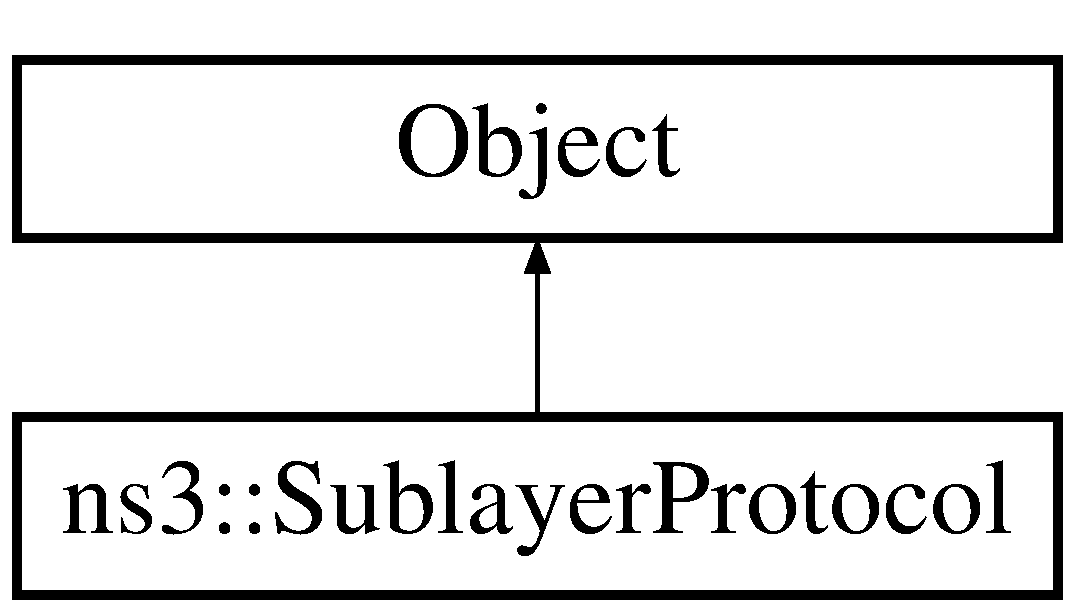
\includegraphics[height=2.000000cm]{classns3_1_1SublayerProtocol}
\end{center}
\end{figure}
\subsection*{Public Member Functions}
\begin{DoxyCompactItemize}
\item 
\hyperlink{classns3_1_1SublayerProtocol_aad21195a67f44c4b4baa72cff040c253}{Sublayer\-Protocol} ()
\item 
virtual \hyperlink{classns3_1_1SublayerProtocol_a0e26c084de2a7c809d8d583c28231215}{$\sim$\-Sublayer\-Protocol} ()
\item 
void \hyperlink{classns3_1_1SublayerProtocol_ae0c35330ed5b9f0c7b109b6ef58b37e6}{Set\-Node} (Ptr$<$ Node $>$ n)
\begin{DoxyCompactList}\small\item\em Set node associated with this stack. \end{DoxyCompactList}\item 
Ptr$<$ Node $>$ \hyperlink{classns3_1_1SublayerProtocol_a6fe8316415eb6ac5d2f41238cba179b2}{Get\-Node} (void)
\begin{DoxyCompactList}\small\item\em Get node associated with this stack. \end{DoxyCompactList}\item 
Ptr$<$ Packet $>$ \hyperlink{classns3_1_1SublayerProtocol_a32f7f8db439df22d32e645249c188de1}{O\-I\-C\-N\-Sublayer\-Check} (Ptr$<$ Packet $>$ packet, Ipv4\-Header ipheader)
\begin{DoxyCompactList}\small\item\em Check for the existence of O\-I\-C\-N Sublayer in the packet, i.\-e. check whether the parameter packet is O\-I\-C\-N Packet or not. This A\-P\-I is called by the \hyperlink{classns3_1_1Ipv4RouterL3Protocol}{Ipv4\-Router\-L3\-Protocol} class whenever it receives a packet. \end{DoxyCompactList}\item 
bool \hyperlink{classns3_1_1SublayerProtocol_adc7c2b22a960eabf0f6a39651b2702f3}{Has\-Sublayer} (Ptr$<$ Packet $>$ packet, Ipv4\-Header ipheader)
\begin{DoxyCompactList}\small\item\em Check whether O\-I\-C\-N Sublayer exists in the I\-P packet. \end{DoxyCompactList}\item 
bool \hyperlink{classns3_1_1SublayerProtocol_ad32d482504ca8f25fa6a710ef8b232f2}{is\-Udp} (Ipv4\-Header ipheader)
\begin{DoxyCompactList}\small\item\em Check whether the Packet is U\-D\-P or not. \end{DoxyCompactList}\item 
bool \hyperlink{classns3_1_1SublayerProtocol_ab20bc8c1fc3159d107d5a3bd41947cdf}{Check\-Cache} (Ptr$<$ Packet $>$ packet1, std\-::string name, Ipv4\-Header ipheader)
\begin{DoxyCompactList}\small\item\em Cache the Application Layer (data) of the Packet after it has been recognized as an O\-I\-C\-N Packet. If the Cache is not full, the data is automatically cached. If the Cache is full, the index (proirity) of the data will determine if some other Cache entry has to be evicted or not. \end{DoxyCompactList}\item 
void \hyperlink{classns3_1_1SublayerProtocol_a5093c7a024d789cab4243e15853cb0db}{Construct\-Packet} (Ptr$<$ Packet $>$ packet, std\-::string Name, uint32\-\_\-t Destination\-Address, uint32\-\_\-t Port\-Number)
\begin{DoxyCompactList}\small\item\em Construct an O\-I\-C\-N Packet for the data retrieved from Cache. This A\-P\-I is required when I\-C\-N Manager requests for data cached in an O\-I\-C\-N Router to be sent to an O\-I\-C\-N Client querying for that content. \end{DoxyCompactList}\item 
void \hyperlink{classns3_1_1SublayerProtocol_a0ad1a28cff0ceeca6086251b4ef26b12}{Construct\-Sublayer} (Ptr$<$ Packet $>$ packet, std\-::string Name)
\begin{DoxyCompactList}\small\item\em Construct the O\-I\-C\-N Sublayer for the O\-I\-C\-N Packet created in Construct\-Packet A\-P\-I, by appending the O\-I\-C\-N Header. \end{DoxyCompactList}\item 
void \hyperlink{classns3_1_1SublayerProtocol_a31827df98334d1c401ad68feaca4105a}{Set\-Udp\-Header} (Udp\-Header header)
\begin{DoxyCompactList}\small\item\em Store the U\-D\-P header of the received packet as a Private Variable 'udp\-\_\-header' in the \hyperlink{classns3_1_1SublayerProtocol}{Sublayer\-Protocol} Object. \end{DoxyCompactList}\item 
void \hyperlink{classns3_1_1SublayerProtocol_a7416f03d29385e56d5b42ed136b7db91}{Set\-O\-I\-C\-N\-Header} (\hyperlink{classns3_1_1OicnHeader}{Oicn\-Header} header)
\begin{DoxyCompactList}\small\item\em Store the O\-I\-C\-N header of the received packet as a Private Variable 'oicn\-\_\-header' in the \hyperlink{classns3_1_1SublayerProtocol}{Sublayer\-Protocol} Object. \end{DoxyCompactList}\item 
void \hyperlink{classns3_1_1SublayerProtocol_ad875af270446269baf99bcaebad48139}{Set\-Cachable} (bool non\-\_\-cachable)
\begin{DoxyCompactList}\small\item\em Set the cachability of the content. \end{DoxyCompactList}\item 
Udp\-Header \hyperlink{classns3_1_1SublayerProtocol_a8fd400667ad5ebdbdfd5d36bf7e592ab}{Get\-Udp\-Header} ()
\begin{DoxyCompactList}\small\item\em Get the U\-D\-P header stored in udp\-\_\-header Private Variable. \end{DoxyCompactList}\item 
\hyperlink{classns3_1_1OicnHeader}{Oicn\-Header} \hyperlink{classns3_1_1SublayerProtocol_a8499790a430e0db48c3117e25f8d42f2}{Get\-O\-I\-C\-N\-Header} ()
\begin{DoxyCompactList}\small\item\em Get the O\-I\-C\-N header stored in oicn\-\_\-header Private Variable. \end{DoxyCompactList}\end{DoxyCompactItemize}
\subsection*{Static Public Member Functions}
\begin{DoxyCompactItemize}
\item 
static Type\-Id \hyperlink{classns3_1_1SublayerProtocol_a98232c65e445399926f5f0cf7b566944}{Get\-Type\-Id} (void)
\begin{DoxyCompactList}\small\item\em Get the type I\-D. \end{DoxyCompactList}\end{DoxyCompactItemize}
\subsection*{Private Attributes}
\begin{DoxyCompactItemize}
\item 
Ptr$<$ Node $>$ \hyperlink{classns3_1_1SublayerProtocol_a4993887dad842a577bdfdfa10cecb7d7}{m\-\_\-node}
\begin{DoxyCompactList}\small\item\em node pointer of current stack \end{DoxyCompactList}\item 
Udp\-Header \hyperlink{classns3_1_1SublayerProtocol_a95b083926386de937c4e9b0a235a4ab8}{udp\-\_\-header}
\begin{DoxyCompactList}\small\item\em U\-D\-P header of the received packet. \end{DoxyCompactList}\item 
\hyperlink{classns3_1_1OicnHeader}{Oicn\-Header} \hyperlink{classns3_1_1SublayerProtocol_a9ceec600a64150a12295c82f01bb8e3c}{oicn\-\_\-header}
\begin{DoxyCompactList}\small\item\em O\-I\-C\-N header of the received packet. \end{DoxyCompactList}\item 
Ptr$<$ Socket $>$ \hyperlink{classns3_1_1SublayerProtocol_a6fb3c36f156ba315448ef4fe95a3c4f6}{m\-\_\-socket}
\begin{DoxyCompactList}\small\item\em socket pointer for the process of sending data queried by O\-I\-C\-N Client \end{DoxyCompactList}\item 
bool \hyperlink{classns3_1_1SublayerProtocol_a829d9ef293fd6c38367143c338850cb7}{m\-\_\-set\-\_\-non\-\_\-cachable}
\begin{DoxyCompactList}\small\item\em indicates whether content is cachable or not \end{DoxyCompactList}\end{DoxyCompactItemize}


\subsection{Detailed Description}
Implements the O\-I\-C\-N Sublayer. 

This class implements the functions that ensures overlay of O\-I\-C\-N Architecture with Current Internet Architecture. It has A\-P\-Is that help in distinguishing O\-I\-C\-N Packets from regular Packets. It also has A\-P\-Is that construct an O\-I\-C\-N Packet and append the O\-I\-C\-N Sublayer to the Packet, whenever data is retrieved from the in the O\-I\-C\-N Router.

This class is instantiated and aggregated to all O\-I\-C\-N Routers in the network, and is not required in any other components of O\-I\-C\-N Architecture.

Note\-: The word Cache here refers to the Named \hyperlink{classns3_1_1Content}{Content} Cache of the I\-C\-N Router. 

\subsection{Constructor \& Destructor Documentation}
\hypertarget{classns3_1_1SublayerProtocol_aad21195a67f44c4b4baa72cff040c253}{\index{ns3\-::\-Sublayer\-Protocol@{ns3\-::\-Sublayer\-Protocol}!Sublayer\-Protocol@{Sublayer\-Protocol}}
\index{Sublayer\-Protocol@{Sublayer\-Protocol}!ns3::SublayerProtocol@{ns3\-::\-Sublayer\-Protocol}}
\subsubsection[{Sublayer\-Protocol}]{\setlength{\rightskip}{0pt plus 5cm}ns3\-::\-Sublayer\-Protocol\-::\-Sublayer\-Protocol (
\begin{DoxyParamCaption}
{}
\end{DoxyParamCaption}
)}}\label{classns3_1_1SublayerProtocol_aad21195a67f44c4b4baa72cff040c253}
\hypertarget{classns3_1_1SublayerProtocol_a0e26c084de2a7c809d8d583c28231215}{\index{ns3\-::\-Sublayer\-Protocol@{ns3\-::\-Sublayer\-Protocol}!$\sim$\-Sublayer\-Protocol@{$\sim$\-Sublayer\-Protocol}}
\index{$\sim$\-Sublayer\-Protocol@{$\sim$\-Sublayer\-Protocol}!ns3::SublayerProtocol@{ns3\-::\-Sublayer\-Protocol}}
\subsubsection[{$\sim$\-Sublayer\-Protocol}]{\setlength{\rightskip}{0pt plus 5cm}ns3\-::\-Sublayer\-Protocol\-::$\sim$\-Sublayer\-Protocol (
\begin{DoxyParamCaption}
{}
\end{DoxyParamCaption}
)\hspace{0.3cm}{\ttfamily [virtual]}}}\label{classns3_1_1SublayerProtocol_a0e26c084de2a7c809d8d583c28231215}


\subsection{Member Function Documentation}
\hypertarget{classns3_1_1SublayerProtocol_ab20bc8c1fc3159d107d5a3bd41947cdf}{\index{ns3\-::\-Sublayer\-Protocol@{ns3\-::\-Sublayer\-Protocol}!Check\-Cache@{Check\-Cache}}
\index{Check\-Cache@{Check\-Cache}!ns3::SublayerProtocol@{ns3\-::\-Sublayer\-Protocol}}
\subsubsection[{Check\-Cache}]{\setlength{\rightskip}{0pt plus 5cm}bool ns3\-::\-Sublayer\-Protocol\-::\-Check\-Cache (
\begin{DoxyParamCaption}
\item[{Ptr$<$ Packet $>$}]{packet1, }
\item[{std\-::string}]{name, }
\item[{Ipv4\-Header}]{ipheader}
\end{DoxyParamCaption}
)}}\label{classns3_1_1SublayerProtocol_ab20bc8c1fc3159d107d5a3bd41947cdf}


Cache the Application Layer (data) of the Packet after it has been recognized as an O\-I\-C\-N Packet. If the Cache is not full, the data is automatically cached. If the Cache is full, the index (proirity) of the data will determine if some other Cache entry has to be evicted or not. 


\begin{DoxyParams}{Parameters}
{\em packet1} & packet received by O\-I\-C\-N Router with its Transport Header removed \\
\hline
{\em name} & name of the corresponding data (or content) of the packet, stored in O\-I\-C\-N Header of the packet. \\
\hline
{\em ipheader} & ip header of the packet \\
\hline
\end{DoxyParams}
\begin{DoxyReturn}{Returns}
true if the data has been cached 
\end{DoxyReturn}
\hypertarget{classns3_1_1SublayerProtocol_a5093c7a024d789cab4243e15853cb0db}{\index{ns3\-::\-Sublayer\-Protocol@{ns3\-::\-Sublayer\-Protocol}!Construct\-Packet@{Construct\-Packet}}
\index{Construct\-Packet@{Construct\-Packet}!ns3::SublayerProtocol@{ns3\-::\-Sublayer\-Protocol}}
\subsubsection[{Construct\-Packet}]{\setlength{\rightskip}{0pt plus 5cm}void ns3\-::\-Sublayer\-Protocol\-::\-Construct\-Packet (
\begin{DoxyParamCaption}
\item[{Ptr$<$ Packet $>$}]{packet, }
\item[{std\-::string}]{Name, }
\item[{uint32\-\_\-t}]{Destination\-Address, }
\item[{uint32\-\_\-t}]{Port\-Number}
\end{DoxyParamCaption}
)}}\label{classns3_1_1SublayerProtocol_a5093c7a024d789cab4243e15853cb0db}


Construct an O\-I\-C\-N Packet for the data retrieved from Cache. This A\-P\-I is required when I\-C\-N Manager requests for data cached in an O\-I\-C\-N Router to be sent to an O\-I\-C\-N Client querying for that content. 


\begin{DoxyParams}{Parameters}
{\em packet} & packet consisting of only the Transport Layer Data. This packet is created after the queried content is searched and found in the Cache by the Cache Manager. \\
\hline
{\em Name} & name of the data retrieved from the Cache. \\
\hline
{\em Destination\-Address} & I\-P address of the O\-I\-C\-N Client querying for that content \\
\hline
{\em Port\-Number} & Port Number of the O\-I\-C\-N Client querying for that content \\
\hline
\end{DoxyParams}
\hypertarget{classns3_1_1SublayerProtocol_a0ad1a28cff0ceeca6086251b4ef26b12}{\index{ns3\-::\-Sublayer\-Protocol@{ns3\-::\-Sublayer\-Protocol}!Construct\-Sublayer@{Construct\-Sublayer}}
\index{Construct\-Sublayer@{Construct\-Sublayer}!ns3::SublayerProtocol@{ns3\-::\-Sublayer\-Protocol}}
\subsubsection[{Construct\-Sublayer}]{\setlength{\rightskip}{0pt plus 5cm}void ns3\-::\-Sublayer\-Protocol\-::\-Construct\-Sublayer (
\begin{DoxyParamCaption}
\item[{Ptr$<$ Packet $>$}]{packet, }
\item[{std\-::string}]{Name}
\end{DoxyParamCaption}
)}}\label{classns3_1_1SublayerProtocol_a0ad1a28cff0ceeca6086251b4ef26b12}


Construct the O\-I\-C\-N Sublayer for the O\-I\-C\-N Packet created in Construct\-Packet A\-P\-I, by appending the O\-I\-C\-N Header. 


\begin{DoxyParams}{Parameters}
{\em packet} & O\-I\-C\-N Packet to which O\-I\-C\-N Header has to be appended. \\
\hline
{\em Name} & name of the content in the O\-I\-C\-N Packet. \\
\hline
\end{DoxyParams}
\hypertarget{classns3_1_1SublayerProtocol_a6fe8316415eb6ac5d2f41238cba179b2}{\index{ns3\-::\-Sublayer\-Protocol@{ns3\-::\-Sublayer\-Protocol}!Get\-Node@{Get\-Node}}
\index{Get\-Node@{Get\-Node}!ns3::SublayerProtocol@{ns3\-::\-Sublayer\-Protocol}}
\subsubsection[{Get\-Node}]{\setlength{\rightskip}{0pt plus 5cm}Ptr$<$ Node $>$ ns3\-::\-Sublayer\-Protocol\-::\-Get\-Node (
\begin{DoxyParamCaption}
\item[{void}]{}
\end{DoxyParamCaption}
)}}\label{classns3_1_1SublayerProtocol_a6fe8316415eb6ac5d2f41238cba179b2}


Get node associated with this stack. 

\begin{DoxyReturn}{Returns}
node of the stack 
\end{DoxyReturn}
\hypertarget{classns3_1_1SublayerProtocol_a8499790a430e0db48c3117e25f8d42f2}{\index{ns3\-::\-Sublayer\-Protocol@{ns3\-::\-Sublayer\-Protocol}!Get\-O\-I\-C\-N\-Header@{Get\-O\-I\-C\-N\-Header}}
\index{Get\-O\-I\-C\-N\-Header@{Get\-O\-I\-C\-N\-Header}!ns3::SublayerProtocol@{ns3\-::\-Sublayer\-Protocol}}
\subsubsection[{Get\-O\-I\-C\-N\-Header}]{\setlength{\rightskip}{0pt plus 5cm}{\bf Oicn\-Header} ns3\-::\-Sublayer\-Protocol\-::\-Get\-O\-I\-C\-N\-Header (
\begin{DoxyParamCaption}
{}
\end{DoxyParamCaption}
)}}\label{classns3_1_1SublayerProtocol_a8499790a430e0db48c3117e25f8d42f2}


Get the O\-I\-C\-N header stored in oicn\-\_\-header Private Variable. 

\begin{DoxyReturn}{Returns}
O\-I\-C\-N\-Header O\-I\-C\-N header stored in oicn\-\_\-header Private Variable 
\end{DoxyReturn}
\hypertarget{classns3_1_1SublayerProtocol_a98232c65e445399926f5f0cf7b566944}{\index{ns3\-::\-Sublayer\-Protocol@{ns3\-::\-Sublayer\-Protocol}!Get\-Type\-Id@{Get\-Type\-Id}}
\index{Get\-Type\-Id@{Get\-Type\-Id}!ns3::SublayerProtocol@{ns3\-::\-Sublayer\-Protocol}}
\subsubsection[{Get\-Type\-Id}]{\setlength{\rightskip}{0pt plus 5cm}Type\-Id ns3\-::\-Sublayer\-Protocol\-::\-Get\-Type\-Id (
\begin{DoxyParamCaption}
\item[{void}]{}
\end{DoxyParamCaption}
)\hspace{0.3cm}{\ttfamily [static]}}}\label{classns3_1_1SublayerProtocol_a98232c65e445399926f5f0cf7b566944}


Get the type I\-D. 

\begin{DoxyReturn}{Returns}
the object Type\-Id 
\end{DoxyReturn}
\hypertarget{classns3_1_1SublayerProtocol_a8fd400667ad5ebdbdfd5d36bf7e592ab}{\index{ns3\-::\-Sublayer\-Protocol@{ns3\-::\-Sublayer\-Protocol}!Get\-Udp\-Header@{Get\-Udp\-Header}}
\index{Get\-Udp\-Header@{Get\-Udp\-Header}!ns3::SublayerProtocol@{ns3\-::\-Sublayer\-Protocol}}
\subsubsection[{Get\-Udp\-Header}]{\setlength{\rightskip}{0pt plus 5cm}Udp\-Header ns3\-::\-Sublayer\-Protocol\-::\-Get\-Udp\-Header (
\begin{DoxyParamCaption}
{}
\end{DoxyParamCaption}
)}}\label{classns3_1_1SublayerProtocol_a8fd400667ad5ebdbdfd5d36bf7e592ab}


Get the U\-D\-P header stored in udp\-\_\-header Private Variable. 

\begin{DoxyReturn}{Returns}
Udp\-Header U\-D\-P header stored in udp\-\_\-header Private Variable 
\end{DoxyReturn}
\hypertarget{classns3_1_1SublayerProtocol_adc7c2b22a960eabf0f6a39651b2702f3}{\index{ns3\-::\-Sublayer\-Protocol@{ns3\-::\-Sublayer\-Protocol}!Has\-Sublayer@{Has\-Sublayer}}
\index{Has\-Sublayer@{Has\-Sublayer}!ns3::SublayerProtocol@{ns3\-::\-Sublayer\-Protocol}}
\subsubsection[{Has\-Sublayer}]{\setlength{\rightskip}{0pt plus 5cm}bool ns3\-::\-Sublayer\-Protocol\-::\-Has\-Sublayer (
\begin{DoxyParamCaption}
\item[{Ptr$<$ Packet $>$}]{packet, }
\item[{Ipv4\-Header}]{ipheader}
\end{DoxyParamCaption}
)}}\label{classns3_1_1SublayerProtocol_adc7c2b22a960eabf0f6a39651b2702f3}


Check whether O\-I\-C\-N Sublayer exists in the I\-P packet. 


\begin{DoxyParams}{Parameters}
{\em packet} & packet received by O\-I\-C\-N Router \\
\hline
{\em ipheader} & I\-P Header of the packet \\
\hline
\end{DoxyParams}
\begin{DoxyReturn}{Returns}
true if O\-I\-C\-N Sublayer exists 
\end{DoxyReturn}
\hypertarget{classns3_1_1SublayerProtocol_ad32d482504ca8f25fa6a710ef8b232f2}{\index{ns3\-::\-Sublayer\-Protocol@{ns3\-::\-Sublayer\-Protocol}!is\-Udp@{is\-Udp}}
\index{is\-Udp@{is\-Udp}!ns3::SublayerProtocol@{ns3\-::\-Sublayer\-Protocol}}
\subsubsection[{is\-Udp}]{\setlength{\rightskip}{0pt plus 5cm}bool ns3\-::\-Sublayer\-Protocol\-::is\-Udp (
\begin{DoxyParamCaption}
\item[{Ipv4\-Header}]{ipheader}
\end{DoxyParamCaption}
)}}\label{classns3_1_1SublayerProtocol_ad32d482504ca8f25fa6a710ef8b232f2}


Check whether the Packet is U\-D\-P or not. 


\begin{DoxyParams}{Parameters}
{\em ipheader} & I\-P Header of the packet \\
\hline
\end{DoxyParams}
\begin{DoxyReturn}{Returns}
true if the Transport Layer used is U\-D\-P 
\end{DoxyReturn}
\hypertarget{classns3_1_1SublayerProtocol_a32f7f8db439df22d32e645249c188de1}{\index{ns3\-::\-Sublayer\-Protocol@{ns3\-::\-Sublayer\-Protocol}!O\-I\-C\-N\-Sublayer\-Check@{O\-I\-C\-N\-Sublayer\-Check}}
\index{O\-I\-C\-N\-Sublayer\-Check@{O\-I\-C\-N\-Sublayer\-Check}!ns3::SublayerProtocol@{ns3\-::\-Sublayer\-Protocol}}
\subsubsection[{O\-I\-C\-N\-Sublayer\-Check}]{\setlength{\rightskip}{0pt plus 5cm}Ptr$<$ Packet $>$ ns3\-::\-Sublayer\-Protocol\-::\-O\-I\-C\-N\-Sublayer\-Check (
\begin{DoxyParamCaption}
\item[{Ptr$<$ Packet $>$}]{packet, }
\item[{Ipv4\-Header}]{ipheader}
\end{DoxyParamCaption}
)}}\label{classns3_1_1SublayerProtocol_a32f7f8db439df22d32e645249c188de1}


Check for the existence of O\-I\-C\-N Sublayer in the packet, i.\-e. check whether the parameter packet is O\-I\-C\-N Packet or not. This A\-P\-I is called by the \hyperlink{classns3_1_1Ipv4RouterL3Protocol}{Ipv4\-Router\-L3\-Protocol} class whenever it receives a packet. 


\begin{DoxyParams}{Parameters}
{\em packet} & packet received by O\-I\-C\-N Router \\
\hline
{\em ipheader} & I\-P Header of the packet \\
\hline
\end{DoxyParams}
\begin{DoxyReturn}{Returns}
the packet after processing 
\end{DoxyReturn}
\hypertarget{classns3_1_1SublayerProtocol_ad875af270446269baf99bcaebad48139}{\index{ns3\-::\-Sublayer\-Protocol@{ns3\-::\-Sublayer\-Protocol}!Set\-Cachable@{Set\-Cachable}}
\index{Set\-Cachable@{Set\-Cachable}!ns3::SublayerProtocol@{ns3\-::\-Sublayer\-Protocol}}
\subsubsection[{Set\-Cachable}]{\setlength{\rightskip}{0pt plus 5cm}void ns3\-::\-Sublayer\-Protocol\-::\-Set\-Cachable (
\begin{DoxyParamCaption}
\item[{bool}]{non\-\_\-cachable}
\end{DoxyParamCaption}
)}}\label{classns3_1_1SublayerProtocol_ad875af270446269baf99bcaebad48139}


Set the cachability of the content. 


\begin{DoxyParams}{Parameters}
{\em non\-\_\-cachable} & indicating whether content is cachable or not \\
\hline
\end{DoxyParams}
\hypertarget{classns3_1_1SublayerProtocol_ae0c35330ed5b9f0c7b109b6ef58b37e6}{\index{ns3\-::\-Sublayer\-Protocol@{ns3\-::\-Sublayer\-Protocol}!Set\-Node@{Set\-Node}}
\index{Set\-Node@{Set\-Node}!ns3::SublayerProtocol@{ns3\-::\-Sublayer\-Protocol}}
\subsubsection[{Set\-Node}]{\setlength{\rightskip}{0pt plus 5cm}void ns3\-::\-Sublayer\-Protocol\-::\-Set\-Node (
\begin{DoxyParamCaption}
\item[{Ptr$<$ Node $>$}]{n}
\end{DoxyParamCaption}
)}}\label{classns3_1_1SublayerProtocol_ae0c35330ed5b9f0c7b109b6ef58b37e6}


Set node associated with this stack. 


\begin{DoxyParams}{Parameters}
{\em node} & node to set \\
\hline
\end{DoxyParams}
\hypertarget{classns3_1_1SublayerProtocol_a7416f03d29385e56d5b42ed136b7db91}{\index{ns3\-::\-Sublayer\-Protocol@{ns3\-::\-Sublayer\-Protocol}!Set\-O\-I\-C\-N\-Header@{Set\-O\-I\-C\-N\-Header}}
\index{Set\-O\-I\-C\-N\-Header@{Set\-O\-I\-C\-N\-Header}!ns3::SublayerProtocol@{ns3\-::\-Sublayer\-Protocol}}
\subsubsection[{Set\-O\-I\-C\-N\-Header}]{\setlength{\rightskip}{0pt plus 5cm}void ns3\-::\-Sublayer\-Protocol\-::\-Set\-O\-I\-C\-N\-Header (
\begin{DoxyParamCaption}
\item[{{\bf Oicn\-Header}}]{header}
\end{DoxyParamCaption}
)}}\label{classns3_1_1SublayerProtocol_a7416f03d29385e56d5b42ed136b7db91}


Store the O\-I\-C\-N header of the received packet as a Private Variable 'oicn\-\_\-header' in the \hyperlink{classns3_1_1SublayerProtocol}{Sublayer\-Protocol} Object. 


\begin{DoxyParams}{Parameters}
{\em header} & O\-I\-C\-N header removed from the received packet \\
\hline
\end{DoxyParams}
\hypertarget{classns3_1_1SublayerProtocol_a31827df98334d1c401ad68feaca4105a}{\index{ns3\-::\-Sublayer\-Protocol@{ns3\-::\-Sublayer\-Protocol}!Set\-Udp\-Header@{Set\-Udp\-Header}}
\index{Set\-Udp\-Header@{Set\-Udp\-Header}!ns3::SublayerProtocol@{ns3\-::\-Sublayer\-Protocol}}
\subsubsection[{Set\-Udp\-Header}]{\setlength{\rightskip}{0pt plus 5cm}void ns3\-::\-Sublayer\-Protocol\-::\-Set\-Udp\-Header (
\begin{DoxyParamCaption}
\item[{Udp\-Header}]{header}
\end{DoxyParamCaption}
)}}\label{classns3_1_1SublayerProtocol_a31827df98334d1c401ad68feaca4105a}


Store the U\-D\-P header of the received packet as a Private Variable 'udp\-\_\-header' in the \hyperlink{classns3_1_1SublayerProtocol}{Sublayer\-Protocol} Object. 


\begin{DoxyParams}{Parameters}
{\em header} & U\-D\-P header removed from the received packet \\
\hline
\end{DoxyParams}


\subsection{Member Data Documentation}
\hypertarget{classns3_1_1SublayerProtocol_a4993887dad842a577bdfdfa10cecb7d7}{\index{ns3\-::\-Sublayer\-Protocol@{ns3\-::\-Sublayer\-Protocol}!m\-\_\-node@{m\-\_\-node}}
\index{m\-\_\-node@{m\-\_\-node}!ns3::SublayerProtocol@{ns3\-::\-Sublayer\-Protocol}}
\subsubsection[{m\-\_\-node}]{\setlength{\rightskip}{0pt plus 5cm}Ptr$<$Node$>$ ns3\-::\-Sublayer\-Protocol\-::m\-\_\-node\hspace{0.3cm}{\ttfamily [private]}}}\label{classns3_1_1SublayerProtocol_a4993887dad842a577bdfdfa10cecb7d7}


node pointer of current stack 

\hypertarget{classns3_1_1SublayerProtocol_a829d9ef293fd6c38367143c338850cb7}{\index{ns3\-::\-Sublayer\-Protocol@{ns3\-::\-Sublayer\-Protocol}!m\-\_\-set\-\_\-non\-\_\-cachable@{m\-\_\-set\-\_\-non\-\_\-cachable}}
\index{m\-\_\-set\-\_\-non\-\_\-cachable@{m\-\_\-set\-\_\-non\-\_\-cachable}!ns3::SublayerProtocol@{ns3\-::\-Sublayer\-Protocol}}
\subsubsection[{m\-\_\-set\-\_\-non\-\_\-cachable}]{\setlength{\rightskip}{0pt plus 5cm}bool ns3\-::\-Sublayer\-Protocol\-::m\-\_\-set\-\_\-non\-\_\-cachable\hspace{0.3cm}{\ttfamily [private]}}}\label{classns3_1_1SublayerProtocol_a829d9ef293fd6c38367143c338850cb7}


indicates whether content is cachable or not 

\hypertarget{classns3_1_1SublayerProtocol_a6fb3c36f156ba315448ef4fe95a3c4f6}{\index{ns3\-::\-Sublayer\-Protocol@{ns3\-::\-Sublayer\-Protocol}!m\-\_\-socket@{m\-\_\-socket}}
\index{m\-\_\-socket@{m\-\_\-socket}!ns3::SublayerProtocol@{ns3\-::\-Sublayer\-Protocol}}
\subsubsection[{m\-\_\-socket}]{\setlength{\rightskip}{0pt plus 5cm}Ptr$<$Socket$>$ ns3\-::\-Sublayer\-Protocol\-::m\-\_\-socket\hspace{0.3cm}{\ttfamily [private]}}}\label{classns3_1_1SublayerProtocol_a6fb3c36f156ba315448ef4fe95a3c4f6}


socket pointer for the process of sending data queried by O\-I\-C\-N Client 

\hypertarget{classns3_1_1SublayerProtocol_a9ceec600a64150a12295c82f01bb8e3c}{\index{ns3\-::\-Sublayer\-Protocol@{ns3\-::\-Sublayer\-Protocol}!oicn\-\_\-header@{oicn\-\_\-header}}
\index{oicn\-\_\-header@{oicn\-\_\-header}!ns3::SublayerProtocol@{ns3\-::\-Sublayer\-Protocol}}
\subsubsection[{oicn\-\_\-header}]{\setlength{\rightskip}{0pt plus 5cm}{\bf Oicn\-Header} ns3\-::\-Sublayer\-Protocol\-::oicn\-\_\-header\hspace{0.3cm}{\ttfamily [private]}}}\label{classns3_1_1SublayerProtocol_a9ceec600a64150a12295c82f01bb8e3c}


O\-I\-C\-N header of the received packet. 

\hypertarget{classns3_1_1SublayerProtocol_a95b083926386de937c4e9b0a235a4ab8}{\index{ns3\-::\-Sublayer\-Protocol@{ns3\-::\-Sublayer\-Protocol}!udp\-\_\-header@{udp\-\_\-header}}
\index{udp\-\_\-header@{udp\-\_\-header}!ns3::SublayerProtocol@{ns3\-::\-Sublayer\-Protocol}}
\subsubsection[{udp\-\_\-header}]{\setlength{\rightskip}{0pt plus 5cm}Udp\-Header ns3\-::\-Sublayer\-Protocol\-::udp\-\_\-header\hspace{0.3cm}{\ttfamily [private]}}}\label{classns3_1_1SublayerProtocol_a95b083926386de937c4e9b0a235a4ab8}


U\-D\-P header of the received packet. 



The documentation for this class was generated from the following files\-:\begin{DoxyCompactItemize}
\item 
model/\hyperlink{sublayer-protocol_8h}{sublayer-\/protocol.\-h}\item 
model/\hyperlink{sublayer-protocol_8cc}{sublayer-\/protocol.\-cc}\end{DoxyCompactItemize}

\chapter{File Documentation}
\hypertarget{oicn-example_8cc}{\section{examples/oicn-\/example.cc File Reference}
\label{oicn-example_8cc}\index{examples/oicn-\/example.\-cc@{examples/oicn-\/example.\-cc}}
}
{\ttfamily \#include $<$iostream$>$}\\*
{\ttfamily \#include $<$fstream$>$}\\*
{\ttfamily \#include $<$string$>$}\\*
{\ttfamily \#include $<$cassert$>$}\\*
{\ttfamily \#include $<$vector$>$}\\*
{\ttfamily \#include \char`\"{}ns3/core-\/module.\-h\char`\"{}}\\*
{\ttfamily \#include \char`\"{}ns3/network-\/module.\-h\char`\"{}}\\*
{\ttfamily \#include \char`\"{}ns3/internet-\/module.\-h\char`\"{}}\\*
{\ttfamily \#include \char`\"{}ns3/point-\/to-\/point-\/module.\-h\char`\"{}}\\*
{\ttfamily \#include \char`\"{}ns3/applications-\/module.\-h\char`\"{}}\\*
{\ttfamily \#include \char`\"{}ns3/o-\/icn-\/module.\-h\char`\"{}}\\*
{\ttfamily \#include \char`\"{}ns3/flow-\/monitor-\/helper.\-h\char`\"{}}\\*
{\ttfamily \#include \char`\"{}ns3/ipv4-\/global-\/routing-\/helper.\-h\char`\"{}}\\*
{\ttfamily \#include $<$unordered\-\_\-map$>$}\\*
\subsection*{Functions}
\begin{DoxyCompactItemize}
\item 
\hyperlink{oicn-example_8cc_ab8dc69a49e07cdbdbba15ec392a6f9de}{N\-S\-\_\-\-L\-O\-G\-\_\-\-C\-O\-M\-P\-O\-N\-E\-N\-T\-\_\-\-D\-E\-F\-I\-N\-E} (\char`\"{}Oicn\-Example\-L\-R\-U\char`\"{})
\item 
int \hyperlink{oicn-example_8cc_a0ddf1224851353fc92bfbff6f499fa97}{main} (int argc, char $\ast$argv\mbox{[}$\,$\mbox{]})
\end{DoxyCompactItemize}


\subsection{Function Documentation}
\hypertarget{oicn-example_8cc_a0ddf1224851353fc92bfbff6f499fa97}{\index{oicn-\/example.\-cc@{oicn-\/example.\-cc}!main@{main}}
\index{main@{main}!oicn-example.cc@{oicn-\/example.\-cc}}
\subsubsection[{main}]{\setlength{\rightskip}{0pt plus 5cm}int main (
\begin{DoxyParamCaption}
\item[{int}]{argc, }
\item[{char $\ast$}]{argv\mbox{[}$\,$\mbox{]}}
\end{DoxyParamCaption}
)}}\label{oicn-example_8cc_a0ddf1224851353fc92bfbff6f499fa97}
\hypertarget{oicn-example_8cc_ab8dc69a49e07cdbdbba15ec392a6f9de}{\index{oicn-\/example.\-cc@{oicn-\/example.\-cc}!N\-S\-\_\-\-L\-O\-G\-\_\-\-C\-O\-M\-P\-O\-N\-E\-N\-T\-\_\-\-D\-E\-F\-I\-N\-E@{N\-S\-\_\-\-L\-O\-G\-\_\-\-C\-O\-M\-P\-O\-N\-E\-N\-T\-\_\-\-D\-E\-F\-I\-N\-E}}
\index{N\-S\-\_\-\-L\-O\-G\-\_\-\-C\-O\-M\-P\-O\-N\-E\-N\-T\-\_\-\-D\-E\-F\-I\-N\-E@{N\-S\-\_\-\-L\-O\-G\-\_\-\-C\-O\-M\-P\-O\-N\-E\-N\-T\-\_\-\-D\-E\-F\-I\-N\-E}!oicn-example.cc@{oicn-\/example.\-cc}}
\subsubsection[{N\-S\-\_\-\-L\-O\-G\-\_\-\-C\-O\-M\-P\-O\-N\-E\-N\-T\-\_\-\-D\-E\-F\-I\-N\-E}]{\setlength{\rightskip}{0pt plus 5cm}N\-S\-\_\-\-L\-O\-G\-\_\-\-C\-O\-M\-P\-O\-N\-E\-N\-T\-\_\-\-D\-E\-F\-I\-N\-E (
\begin{DoxyParamCaption}
\item[{\char`\"{}Oicn\-Example\-L\-R\-U\char`\"{}}]{}
\end{DoxyParamCaption}
)}}\label{oicn-example_8cc_ab8dc69a49e07cdbdbba15ec392a6f9de}

\hypertarget{oicn-application-helper_8cc}{\section{helper/oicn-\/application-\/helper.cc File Reference}
\label{oicn-application-helper_8cc}\index{helper/oicn-\/application-\/helper.\-cc@{helper/oicn-\/application-\/helper.\-cc}}
}
{\ttfamily \#include \char`\"{}ns3/icn-\/router.\-h\char`\"{}}\\*
{\ttfamily \#include \char`\"{}ns3/type-\/id.\-h\char`\"{}}\\*
{\ttfamily \#include \char`\"{}oicn-\/application-\/helper.\-h\char`\"{}}\\*
{\ttfamily \#include \char`\"{}ns3/log.\-h\char`\"{}}\\*
{\ttfamily \#include \char`\"{}ns3/node.\-h\char`\"{}}\\*
{\ttfamily \#include \char`\"{}ns3/uinteger.\-h\char`\"{}}\\*
{\ttfamily \#include \char`\"{}ns3/oicn-\/client-\/application.\-h\char`\"{}}\\*
{\ttfamily \#include \char`\"{}ns3/oicn-\/zipf-\/client.\-h\char`\"{}}\\*
{\ttfamily \#include \char`\"{}ns3/oicn-\/server-\/application.\-h\char`\"{}}\\*
{\ttfamily \#include \char`\"{}ns3/icn-\/manager.\-h\char`\"{}}\\*
{\ttfamily \#include \char`\"{}ns3/content.\-h\char`\"{}}\\*
{\ttfamily \#include $<$vector$>$}\\*
\subsection*{Namespaces}
\begin{DoxyCompactItemize}
\item 
\hyperlink{namespacens3}{ns3}
\end{DoxyCompactItemize}
\subsection*{Functions}
\begin{DoxyCompactItemize}
\item 
\hyperlink{oicn-application-helper_8cc_a619ef641822f605d852bad6926ce2041}{N\-S\-\_\-\-L\-O\-G\-\_\-\-C\-O\-M\-P\-O\-N\-E\-N\-T\-\_\-\-D\-E\-F\-I\-N\-E} (\char`\"{}O\-I\-C\-N\-App\-Helper\char`\"{})
\end{DoxyCompactItemize}


\subsection{Function Documentation}
\hypertarget{oicn-application-helper_8cc_a619ef641822f605d852bad6926ce2041}{\index{oicn-\/application-\/helper.\-cc@{oicn-\/application-\/helper.\-cc}!N\-S\-\_\-\-L\-O\-G\-\_\-\-C\-O\-M\-P\-O\-N\-E\-N\-T\-\_\-\-D\-E\-F\-I\-N\-E@{N\-S\-\_\-\-L\-O\-G\-\_\-\-C\-O\-M\-P\-O\-N\-E\-N\-T\-\_\-\-D\-E\-F\-I\-N\-E}}
\index{N\-S\-\_\-\-L\-O\-G\-\_\-\-C\-O\-M\-P\-O\-N\-E\-N\-T\-\_\-\-D\-E\-F\-I\-N\-E@{N\-S\-\_\-\-L\-O\-G\-\_\-\-C\-O\-M\-P\-O\-N\-E\-N\-T\-\_\-\-D\-E\-F\-I\-N\-E}!oicn-application-helper.cc@{oicn-\/application-\/helper.\-cc}}
\subsubsection[{N\-S\-\_\-\-L\-O\-G\-\_\-\-C\-O\-M\-P\-O\-N\-E\-N\-T\-\_\-\-D\-E\-F\-I\-N\-E}]{\setlength{\rightskip}{0pt plus 5cm}N\-S\-\_\-\-L\-O\-G\-\_\-\-C\-O\-M\-P\-O\-N\-E\-N\-T\-\_\-\-D\-E\-F\-I\-N\-E (
\begin{DoxyParamCaption}
\item[{\char`\"{}O\-I\-C\-N\-App\-Helper\char`\"{}}]{}
\end{DoxyParamCaption}
)}}\label{oicn-application-helper_8cc_a619ef641822f605d852bad6926ce2041}

\hypertarget{oicn-application-helper_8h}{\section{helper/oicn-\/application-\/helper.h File Reference}
\label{oicn-application-helper_8h}\index{helper/oicn-\/application-\/helper.\-h@{helper/oicn-\/application-\/helper.\-h}}
}
{\ttfamily \#include $<$stdint.\-h$>$}\\*
{\ttfamily \#include $<$vector$>$}\\*
{\ttfamily \#include \char`\"{}ns3/uinteger.\-h\char`\"{}}\\*
{\ttfamily \#include \char`\"{}ns3/application.\-h\char`\"{}}\\*
{\ttfamily \#include \char`\"{}ns3/application-\/container.\-h\char`\"{}}\\*
{\ttfamily \#include \char`\"{}ns3/node-\/container.\-h\char`\"{}}\\*
{\ttfamily \#include \char`\"{}ns3/object-\/factory.\-h\char`\"{}}\\*
{\ttfamily \#include \char`\"{}ns3/ipv4-\/address.\-h\char`\"{}}\\*
{\ttfamily \#include \char`\"{}ns3/node.\-h\char`\"{}}\\*
\subsection*{Classes}
\begin{DoxyCompactItemize}
\item 
class \hyperlink{classns3_1_1OicnServerHelper}{ns3\-::\-Oicn\-Server\-Helper}
\begin{DoxyCompactList}\small\item\em Create a O\-I\-C\-N Server application. I\-C\-N Manager direct O\-I\-C\-N server to send requested content to O\-I\-C\-N client. \end{DoxyCompactList}\item 
class \hyperlink{classns3_1_1IcnManagerHelper}{ns3\-::\-Icn\-Manager\-Helper}
\begin{DoxyCompactList}\small\item\em Create an application which resolve the name request (check whether content present at I\-C\-N router or server) and forward request to source of content (I\-C\-N router or server). \end{DoxyCompactList}\item 
class \hyperlink{classns3_1_1OicnClientHelpher}{ns3\-::\-Oicn\-Client\-Helpher}
\begin{DoxyCompactList}\small\item\em Create a O\-I\-C\-N Client application which send content name resolution request to I\-C\-N Manager. I\-C\-N Manager direct the content request to I\-C\-N source (O\-I\-C\-N server or I\-C\-N router) which reply to O\-I\-C\-N client with requested content. \end{DoxyCompactList}\item 
class \hyperlink{classns3_1_1OicnZipfClientHelper}{ns3\-::\-Oicn\-Zipf\-Client\-Helper}
\begin{DoxyCompactList}\small\item\em Create O\-I\-C\-N Zipf Client, it generates request for the contents following Zipf-\/\-Mandelbrot Distribution. Here is the explanation of Zipf-\/\-Mandelbrot Distribution\-: \href{http://en.wikipedia.org/wiki/Zipf%E2%80%93Mandelbrot_law}{\tt http\-://en.\-wikipedia.\-org/wiki/\-Zipf\%\-E2\%80\%93\-Mandelbrot\-\_\-law}. Client application send name resolution to I\-C\-N Manager. I\-C\-N Manager do the name resolution and direct source (I\-C\-N router or server) to send the content to the O\-I\-C\-N Zipf Client. \end{DoxyCompactList}\item 
class \hyperlink{classns3_1_1IcnRouterHelpher}{ns3\-::\-Icn\-Router\-Helpher}
\begin{DoxyCompactList}\small\item\em I\-C\-N Router has the capability to cache the contents. \end{DoxyCompactList}\end{DoxyCompactItemize}
\subsection*{Namespaces}
\begin{DoxyCompactItemize}
\item 
\hyperlink{namespacens3}{ns3}
\end{DoxyCompactItemize}

\hypertarget{router-stack-helper_8cc}{\section{helper/router-\/stack-\/helper.cc File Reference}
\label{router-stack-helper_8cc}\index{helper/router-\/stack-\/helper.\-cc@{helper/router-\/stack-\/helper.\-cc}}
}
{\ttfamily \#include \char`\"{}ns3/assert.\-h\char`\"{}}\\*
{\ttfamily \#include \char`\"{}ns3/log.\-h\char`\"{}}\\*
{\ttfamily \#include \char`\"{}ns3/object.\-h\char`\"{}}\\*
{\ttfamily \#include \char`\"{}ns3/names.\-h\char`\"{}}\\*
{\ttfamily \#include \char`\"{}ns3/ipv4.\-h\char`\"{}}\\*
{\ttfamily \#include \char`\"{}ns3/packet-\/socket-\/factory.\-h\char`\"{}}\\*
{\ttfamily \#include \char`\"{}ns3/config.\-h\char`\"{}}\\*
{\ttfamily \#include \char`\"{}ns3/simulator.\-h\char`\"{}}\\*
{\ttfamily \#include \char`\"{}ns3/string.\-h\char`\"{}}\\*
{\ttfamily \#include \char`\"{}ns3/net-\/device.\-h\char`\"{}}\\*
{\ttfamily \#include \char`\"{}ns3/callback.\-h\char`\"{}}\\*
{\ttfamily \#include \char`\"{}ns3/node.\-h\char`\"{}}\\*
{\ttfamily \#include \char`\"{}ns3/node-\/list.\-h\char`\"{}}\\*
{\ttfamily \#include \char`\"{}ns3/core-\/config.\-h\char`\"{}}\\*
{\ttfamily \#include \char`\"{}ns3/arp-\/l3-\/protocol.\-h\char`\"{}}\\*
{\ttfamily \#include \char`\"{}ns3/named-\/content-\/cache.\-h\char`\"{}}\\*
{\ttfamily \#include \char`\"{}router-\/stack-\/helper.\-h\char`\"{}}\\*
{\ttfamily \#include \char`\"{}ns3/sublayer-\/protocol.\-h\char`\"{}}\\*
{\ttfamily \#include \char`\"{}ns3/ipv4-\/global-\/routing.\-h\char`\"{}}\\*
{\ttfamily \#include \char`\"{}ns3/ipv4-\/list-\/routing-\/helper.\-h\char`\"{}}\\*
{\ttfamily \#include \char`\"{}ns3/ipv4-\/static-\/routing-\/helper.\-h\char`\"{}}\\*
{\ttfamily \#include \char`\"{}ns3/ipv4-\/global-\/routing-\/helper.\-h\char`\"{}}\\*
{\ttfamily \#include \char`\"{}ns3/global-\/router-\/interface.\-h\char`\"{}}\\*
{\ttfamily \#include $<$limits$>$}\\*
{\ttfamily \#include $<$map$>$}\\*
\subsection*{Namespaces}
\begin{DoxyCompactItemize}
\item 
\hyperlink{namespacens3}{ns3}
\end{DoxyCompactItemize}
\subsection*{Macros}
\begin{DoxyCompactItemize}
\item 
\#define \hyperlink{router-stack-helper_8cc_a7db88cb02fe5c738db27431496b7131e}{I\-N\-T\-E\-R\-F\-A\-C\-E\-\_\-\-C\-O\-N\-T\-E\-X\-T}
\end{DoxyCompactItemize}
\subsection*{Typedefs}
\begin{DoxyCompactItemize}
\item 
typedef std\-::pair$<$ Ptr$<$ Ipv4 $>$\\*
, uint32\-\_\-t $>$ \hyperlink{namespacens3_a83e2603870381affabd5ca766d17daff}{ns3\-::\-Interface\-Pair\-Ipv4}
\item 
typedef std\-::map\\*
$<$ Interface\-Pair\-Ipv4, Ptr\\*
$<$ Pcap\-File\-Wrapper $>$ $>$ \hyperlink{namespacens3_ab14a5629528234e6f76ad3bb180022fe}{ns3\-::\-Interface\-File\-Map\-Ipv4}
\item 
typedef std\-::map\\*
$<$ Interface\-Pair\-Ipv4, Ptr\\*
$<$ Output\-Stream\-Wrapper $>$ $>$ \hyperlink{namespacens3_a5634ac4e27d952132fba4cd906d4ebd3}{ns3\-::\-Interface\-Stream\-Map\-Ipv4}
\end{DoxyCompactItemize}
\subsection*{Functions}
\begin{DoxyCompactItemize}
\item 
\hyperlink{router-stack-helper_8cc_ab2435b2b13a2f2a29451f2630b953daf}{N\-S\-\_\-\-L\-O\-G\-\_\-\-C\-O\-M\-P\-O\-N\-E\-N\-T\-\_\-\-D\-E\-F\-I\-N\-E} (\char`\"{}Router\-Stack\-Helper\char`\"{})
\item 
static void \hyperlink{namespacens3_acde124208ae741ae241b61b9a22ead8d}{ns3\-::\-Ipv4\-Router\-L3\-Protocol\-Rx\-Tx\-Sink} (Ptr$<$ const Packet $>$ p, Ptr$<$ Ipv4 $>$ ipv4, uint32\-\_\-t interface)
\end{DoxyCompactItemize}
\subsection*{Variables}
\begin{DoxyCompactItemize}
\item 
static Interface\-File\-Map\-Ipv4 \hyperlink{namespacens3_ac1df4c15ca334fd8713f6600d097c1a6}{ns3\-::g\-\_\-interface\-File\-Map\-Ipv4}
\item 
static Interface\-Stream\-Map\-Ipv4 \hyperlink{namespacens3_ad7720e08dcb21331d85c00128abc175a}{ns3\-::g\-\_\-interface\-Stream\-Map\-Ipv4}
\end{DoxyCompactItemize}


\subsection{Macro Definition Documentation}
\hypertarget{router-stack-helper_8cc_a7db88cb02fe5c738db27431496b7131e}{\index{router-\/stack-\/helper.\-cc@{router-\/stack-\/helper.\-cc}!I\-N\-T\-E\-R\-F\-A\-C\-E\-\_\-\-C\-O\-N\-T\-E\-X\-T@{I\-N\-T\-E\-R\-F\-A\-C\-E\-\_\-\-C\-O\-N\-T\-E\-X\-T}}
\index{I\-N\-T\-E\-R\-F\-A\-C\-E\-\_\-\-C\-O\-N\-T\-E\-X\-T@{I\-N\-T\-E\-R\-F\-A\-C\-E\-\_\-\-C\-O\-N\-T\-E\-X\-T}!router-stack-helper.cc@{router-\/stack-\/helper.\-cc}}
\subsubsection[{I\-N\-T\-E\-R\-F\-A\-C\-E\-\_\-\-C\-O\-N\-T\-E\-X\-T}]{\setlength{\rightskip}{0pt plus 5cm}\#define I\-N\-T\-E\-R\-F\-A\-C\-E\-\_\-\-C\-O\-N\-T\-E\-X\-T}}\label{router-stack-helper_8cc_a7db88cb02fe5c738db27431496b7131e}


\subsection{Function Documentation}
\hypertarget{router-stack-helper_8cc_ab2435b2b13a2f2a29451f2630b953daf}{\index{router-\/stack-\/helper.\-cc@{router-\/stack-\/helper.\-cc}!N\-S\-\_\-\-L\-O\-G\-\_\-\-C\-O\-M\-P\-O\-N\-E\-N\-T\-\_\-\-D\-E\-F\-I\-N\-E@{N\-S\-\_\-\-L\-O\-G\-\_\-\-C\-O\-M\-P\-O\-N\-E\-N\-T\-\_\-\-D\-E\-F\-I\-N\-E}}
\index{N\-S\-\_\-\-L\-O\-G\-\_\-\-C\-O\-M\-P\-O\-N\-E\-N\-T\-\_\-\-D\-E\-F\-I\-N\-E@{N\-S\-\_\-\-L\-O\-G\-\_\-\-C\-O\-M\-P\-O\-N\-E\-N\-T\-\_\-\-D\-E\-F\-I\-N\-E}!router-stack-helper.cc@{router-\/stack-\/helper.\-cc}}
\subsubsection[{N\-S\-\_\-\-L\-O\-G\-\_\-\-C\-O\-M\-P\-O\-N\-E\-N\-T\-\_\-\-D\-E\-F\-I\-N\-E}]{\setlength{\rightskip}{0pt plus 5cm}N\-S\-\_\-\-L\-O\-G\-\_\-\-C\-O\-M\-P\-O\-N\-E\-N\-T\-\_\-\-D\-E\-F\-I\-N\-E (
\begin{DoxyParamCaption}
\item[{\char`\"{}Router\-Stack\-Helper\char`\"{}}]{}
\end{DoxyParamCaption}
)}}\label{router-stack-helper_8cc_ab2435b2b13a2f2a29451f2630b953daf}

\hypertarget{router-stack-helper_8h}{\section{helper/router-\/stack-\/helper.h File Reference}
\label{router-stack-helper_8h}\index{helper/router-\/stack-\/helper.\-h@{helper/router-\/stack-\/helper.\-h}}
}
{\ttfamily \#include $<$string$>$}\\*
{\ttfamily \#include \char`\"{}ns3/node-\/container.\-h\char`\"{}}\\*
{\ttfamily \#include \char`\"{}ns3/net-\/device-\/container.\-h\char`\"{}}\\*
{\ttfamily \#include \char`\"{}ns3/packet.\-h\char`\"{}}\\*
{\ttfamily \#include \char`\"{}ns3/ptr.\-h\char`\"{}}\\*
{\ttfamily \#include \char`\"{}ns3/object-\/factory.\-h\char`\"{}}\\*
{\ttfamily \#include \char`\"{}ns3/ipv4-\/router-\/l3-\/protocol.\-h\char`\"{}}\\*
{\ttfamily \#include \char`\"{}ns3/internet-\/trace-\/helper.\-h\char`\"{}}\\*
\subsection*{Classes}
\begin{DoxyCompactItemize}
\item 
class \hyperlink{classns3_1_1RouterStackHelper}{ns3\-::\-Router\-Stack\-Helper}
\begin{DoxyCompactList}\small\item\em Aggregate I\-P/\-T\-C\-P/\-U\-D\-P and Caching functionality to only I\-C\-N Routers in the Network. \end{DoxyCompactList}\end{DoxyCompactItemize}
\subsection*{Namespaces}
\begin{DoxyCompactItemize}
\item 
\hyperlink{namespacens3}{ns3}
\end{DoxyCompactItemize}

\hypertarget{cache-manager_8cc}{\section{model/cache-\/manager.cc File Reference}
\label{cache-manager_8cc}\index{model/cache-\/manager.\-cc@{model/cache-\/manager.\-cc}}
}
{\ttfamily \#include \char`\"{}ns3/type-\/id.\-h\char`\"{}}\\*
{\ttfamily \#include \char`\"{}ns3/type-\/name.\-h\char`\"{}}\\*
{\ttfamily \#include \char`\"{}cache-\/manager.\-h\char`\"{}}\\*
{\ttfamily \#include \char`\"{}icn-\/manager.\-h\char`\"{}}\\*
{\ttfamily \#include \char`\"{}named-\/content-\/cache.\-h\char`\"{}}\\*
{\ttfamily \#include \char`\"{}ns3/ptr.\-h\char`\"{}}\\*
{\ttfamily \#include \char`\"{}ns3/log.\-h\char`\"{}}\\*
{\ttfamily \#include \char`\"{}ns3/packet.\-h\char`\"{}}\\*
{\ttfamily \#include \char`\"{}sublayer-\/protocol.\-h\char`\"{}}\\*
{\ttfamily \#include \char`\"{}ns3/ipv4-\/header.\-h\char`\"{}}\\*
{\ttfamily \#include \char`\"{}ns3/ipv4-\/address.\-h\char`\"{}}\\*
{\ttfamily \#include \char`\"{}ns3/ipv4.\-h\char`\"{}}\\*
\subsection*{Namespaces}
\begin{DoxyCompactItemize}
\item 
\hyperlink{namespacens3}{ns3}
\end{DoxyCompactItemize}
\subsection*{Functions}
\begin{DoxyCompactItemize}
\item 
\hyperlink{cache-manager_8cc_a6ce37ef34f486407a4820d76f400d96f}{N\-S\-\_\-\-L\-O\-G\-\_\-\-C\-O\-M\-P\-O\-N\-E\-N\-T\-\_\-\-D\-E\-F\-I\-N\-E} (\char`\"{}Cache\-Manager\char`\"{})
\item 
\hyperlink{namespacens3_a8da84469566489f34d19639bac5068a9}{ns3\-::\-N\-S\-\_\-\-O\-B\-J\-E\-C\-T\-\_\-\-E\-N\-S\-U\-R\-E\-\_\-\-R\-E\-G\-I\-S\-T\-E\-R\-E\-D} (Cache\-Manager)
\end{DoxyCompactItemize}


\subsection{Function Documentation}
\hypertarget{cache-manager_8cc_a6ce37ef34f486407a4820d76f400d96f}{\index{cache-\/manager.\-cc@{cache-\/manager.\-cc}!N\-S\-\_\-\-L\-O\-G\-\_\-\-C\-O\-M\-P\-O\-N\-E\-N\-T\-\_\-\-D\-E\-F\-I\-N\-E@{N\-S\-\_\-\-L\-O\-G\-\_\-\-C\-O\-M\-P\-O\-N\-E\-N\-T\-\_\-\-D\-E\-F\-I\-N\-E}}
\index{N\-S\-\_\-\-L\-O\-G\-\_\-\-C\-O\-M\-P\-O\-N\-E\-N\-T\-\_\-\-D\-E\-F\-I\-N\-E@{N\-S\-\_\-\-L\-O\-G\-\_\-\-C\-O\-M\-P\-O\-N\-E\-N\-T\-\_\-\-D\-E\-F\-I\-N\-E}!cache-manager.cc@{cache-\/manager.\-cc}}
\subsubsection[{N\-S\-\_\-\-L\-O\-G\-\_\-\-C\-O\-M\-P\-O\-N\-E\-N\-T\-\_\-\-D\-E\-F\-I\-N\-E}]{\setlength{\rightskip}{0pt plus 5cm}N\-S\-\_\-\-L\-O\-G\-\_\-\-C\-O\-M\-P\-O\-N\-E\-N\-T\-\_\-\-D\-E\-F\-I\-N\-E (
\begin{DoxyParamCaption}
\item[{\char`\"{}Cache\-Manager\char`\"{}}]{}
\end{DoxyParamCaption}
)}}\label{cache-manager_8cc_a6ce37ef34f486407a4820d76f400d96f}

\hypertarget{cache-manager_8h}{\section{model/cache-\/manager.h File Reference}
\label{cache-manager_8h}\index{model/cache-\/manager.\-h@{model/cache-\/manager.\-h}}
}
{\ttfamily \#include \char`\"{}ns3/ptr.\-h\char`\"{}}\\*
{\ttfamily \#include \char`\"{}ns3/packet.\-h\char`\"{}}\\*
{\ttfamily \#include \char`\"{}ns3/ipv4-\/header.\-h\char`\"{}}\\*
{\ttfamily \#include \char`\"{}ns3/type-\/name.\-h\char`\"{}}\\*
{\ttfamily \#include \char`\"{}ns3/type-\/id.\-h\char`\"{}}\\*
{\ttfamily \#include \char`\"{}ns3/object.\-h\char`\"{}}\\*
{\ttfamily \#include \char`\"{}ns3/node.\-h\char`\"{}}\\*
{\ttfamily \#include $<$stdint.\-h$>$}\\*
\subsection*{Classes}
\begin{DoxyCompactItemize}
\item 
class \hyperlink{classns3_1_1CacheManager}{ns3\-::\-Cache\-Manager}
\begin{DoxyCompactList}\small\item\em Manages the Named \hyperlink{classns3_1_1Content}{Content} Cache of an O\-I\-C\-N Router. \end{DoxyCompactList}\end{DoxyCompactItemize}
\subsection*{Namespaces}
\begin{DoxyCompactItemize}
\item 
\hyperlink{namespacens3}{ns3}
\end{DoxyCompactItemize}

\hypertarget{cache-with-fifo_8cc}{\section{model/cache-\/with-\/fifo.cc File Reference}
\label{cache-with-fifo_8cc}\index{model/cache-\/with-\/fifo.\-cc@{model/cache-\/with-\/fifo.\-cc}}
}
{\ttfamily \#include \char`\"{}ns3/type-\/id.\-h\char`\"{}}\\*
{\ttfamily \#include \char`\"{}ns3/type-\/name.\-h\char`\"{}}\\*
{\ttfamily \#include \char`\"{}ns3/ptr.\-h\char`\"{}}\\*
{\ttfamily \#include \char`\"{}ns3/log.\-h\char`\"{}}\\*
{\ttfamily \#include \char`\"{}ns3/packet.\-h\char`\"{}}\\*
{\ttfamily \#include \char`\"{}ns3/simulator.\-h\char`\"{}}\\*
{\ttfamily \#include \char`\"{}named-\/content-\/cache-\/entry.\-h\char`\"{}}\\*
{\ttfamily \#include \char`\"{}cache-\/with-\/fifo.\-h\char`\"{}}\\*
{\ttfamily \#include $<$stdint.\-h$>$}\\*
{\ttfamily \#include $<$string$>$}\\*
{\ttfamily \#include $<$utility$>$}\\*
{\ttfamily \#include $<$cstring$>$}\\*
{\ttfamily \#include $<$iostream$>$}\\*
{\ttfamily \#include $<$boost/unordered\-\_\-map.\-hpp$>$}\\*
{\ttfamily \#include $<$boost/bimap.\-hpp$>$}\\*
{\ttfamily \#include $<$boost/bimap/bimap.\-hpp$>$}\\*
{\ttfamily \#include $<$boost/bimap/set\-\_\-of.\-hpp$>$}\\*
{\ttfamily \#include $<$boost/bimap/detail/bimap\-\_\-core.\-hpp$>$}\\*
{\ttfamily \#include $<$boost/bimap/unordered\-\_\-set\-\_\-of.\-hpp$>$}\\*
\subsection*{Namespaces}
\begin{DoxyCompactItemize}
\item 
\hyperlink{namespacens3}{ns3}
\end{DoxyCompactItemize}
\subsection*{Functions}
\begin{DoxyCompactItemize}
\item 
\hyperlink{cache-with-fifo_8cc_a08b6df7434f51173640add58f982ab07}{N\-S\-\_\-\-L\-O\-G\-\_\-\-C\-O\-M\-P\-O\-N\-E\-N\-T\-\_\-\-D\-E\-F\-I\-N\-E} (\char`\"{}Cache\-With\-Fifo\char`\"{})
\item 
\hyperlink{namespacens3_aecd9f25af1b30fe642f6ecdfc1eac7fd}{ns3\-::\-N\-S\-\_\-\-O\-B\-J\-E\-C\-T\-\_\-\-E\-N\-S\-U\-R\-E\-\_\-\-R\-E\-G\-I\-S\-T\-E\-R\-E\-D} (Cache\-With\-Fifo)
\end{DoxyCompactItemize}


\subsection{Function Documentation}
\hypertarget{cache-with-fifo_8cc_a08b6df7434f51173640add58f982ab07}{\index{cache-\/with-\/fifo.\-cc@{cache-\/with-\/fifo.\-cc}!N\-S\-\_\-\-L\-O\-G\-\_\-\-C\-O\-M\-P\-O\-N\-E\-N\-T\-\_\-\-D\-E\-F\-I\-N\-E@{N\-S\-\_\-\-L\-O\-G\-\_\-\-C\-O\-M\-P\-O\-N\-E\-N\-T\-\_\-\-D\-E\-F\-I\-N\-E}}
\index{N\-S\-\_\-\-L\-O\-G\-\_\-\-C\-O\-M\-P\-O\-N\-E\-N\-T\-\_\-\-D\-E\-F\-I\-N\-E@{N\-S\-\_\-\-L\-O\-G\-\_\-\-C\-O\-M\-P\-O\-N\-E\-N\-T\-\_\-\-D\-E\-F\-I\-N\-E}!cache-with-fifo.cc@{cache-\/with-\/fifo.\-cc}}
\subsubsection[{N\-S\-\_\-\-L\-O\-G\-\_\-\-C\-O\-M\-P\-O\-N\-E\-N\-T\-\_\-\-D\-E\-F\-I\-N\-E}]{\setlength{\rightskip}{0pt plus 5cm}N\-S\-\_\-\-L\-O\-G\-\_\-\-C\-O\-M\-P\-O\-N\-E\-N\-T\-\_\-\-D\-E\-F\-I\-N\-E (
\begin{DoxyParamCaption}
\item[{\char`\"{}Cache\-With\-Fifo\char`\"{}}]{}
\end{DoxyParamCaption}
)}}\label{cache-with-fifo_8cc_a08b6df7434f51173640add58f982ab07}

\hypertarget{cache-with-fifo_8h}{\section{model/cache-\/with-\/fifo.h File Reference}
\label{cache-with-fifo_8h}\index{model/cache-\/with-\/fifo.\-h@{model/cache-\/with-\/fifo.\-h}}
}
{\ttfamily \#include \char`\"{}ns3/ptr.\-h\char`\"{}}\\*
{\ttfamily \#include \char`\"{}ns3/packet.\-h\char`\"{}}\\*
{\ttfamily \#include \char`\"{}ns3/node.\-h\char`\"{}}\\*
{\ttfamily \#include \char`\"{}named-\/content-\/cache-\/entry.\-h\char`\"{}}\\*
{\ttfamily \#include \char`\"{}named-\/content-\/cache.\-h\char`\"{}}\\*
{\ttfamily \#include \char`\"{}ns3/type-\/name.\-h\char`\"{}}\\*
{\ttfamily \#include \char`\"{}ns3/object.\-h\char`\"{}}\\*
{\ttfamily \#include \char`\"{}ns3/type-\/id.\-h\char`\"{}}\\*
{\ttfamily \#include \char`\"{}ns3/ipv4-\/header.\-h\char`\"{}}\\*
{\ttfamily \#include $<$stdint.\-h$>$}\\*
{\ttfamily \#include $<$string$>$}\\*
{\ttfamily \#include $<$boost/unordered\-\_\-map.\-hpp$>$}\\*
{\ttfamily \#include $<$boost/bimap.\-hpp$>$}\\*
{\ttfamily \#include $<$boost/bimap/bimap.\-hpp$>$}\\*
{\ttfamily \#include $<$boost/bimap/set\-\_\-of.\-hpp$>$}\\*
{\ttfamily \#include $<$boost/bimap/detail/bimap\-\_\-core.\-hpp$>$}\\*
{\ttfamily \#include $<$boost/bimap/unordered\-\_\-set\-\_\-of.\-hpp$>$}\\*
\subsection*{Classes}
\begin{DoxyCompactItemize}
\item 
class \hyperlink{classns3_1_1CacheWithFifo}{ns3\-::\-Cache\-With\-Fifo}
\begin{DoxyCompactList}\small\item\em This class implements the first in first out caching policy. \end{DoxyCompactList}\end{DoxyCompactItemize}
\subsection*{Namespaces}
\begin{DoxyCompactItemize}
\item 
\hyperlink{namespacens3}{ns3}
\end{DoxyCompactItemize}

\hypertarget{cache-with-lfu_8cc}{\section{model/cache-\/with-\/lfu.cc File Reference}
\label{cache-with-lfu_8cc}\index{model/cache-\/with-\/lfu.\-cc@{model/cache-\/with-\/lfu.\-cc}}
}
{\ttfamily \#include \char`\"{}ns3/type-\/id.\-h\char`\"{}}\\*
{\ttfamily \#include \char`\"{}ns3/type-\/name.\-h\char`\"{}}\\*
{\ttfamily \#include \char`\"{}ns3/ptr.\-h\char`\"{}}\\*
{\ttfamily \#include \char`\"{}ns3/log.\-h\char`\"{}}\\*
{\ttfamily \#include \char`\"{}ns3/packet.\-h\char`\"{}}\\*
{\ttfamily \#include \char`\"{}ns3/simulator.\-h\char`\"{}}\\*
{\ttfamily \#include \char`\"{}named-\/content-\/cache-\/entry.\-h\char`\"{}}\\*
{\ttfamily \#include \char`\"{}cache-\/with-\/lfu.\-h\char`\"{}}\\*
{\ttfamily \#include $<$stdint.\-h$>$}\\*
{\ttfamily \#include $<$string$>$}\\*
{\ttfamily \#include $<$utility$>$}\\*
{\ttfamily \#include $<$cstring$>$}\\*
{\ttfamily \#include $<$iostream$>$}\\*
{\ttfamily \#include $<$boost/unordered\-\_\-map.\-hpp$>$}\\*
{\ttfamily \#include $<$boost/bimap.\-hpp$>$}\\*
{\ttfamily \#include $<$boost/bimap/bimap.\-hpp$>$}\\*
{\ttfamily \#include $<$boost/bimap/set\-\_\-of.\-hpp$>$}\\*
{\ttfamily \#include $<$boost/bimap/detail/bimap\-\_\-core.\-hpp$>$}\\*
{\ttfamily \#include $<$boost/bimap/unordered\-\_\-set\-\_\-of.\-hpp$>$}\\*
\subsection*{Namespaces}
\begin{DoxyCompactItemize}
\item 
\hyperlink{namespacens3}{ns3}
\end{DoxyCompactItemize}
\subsection*{Functions}
\begin{DoxyCompactItemize}
\item 
\hyperlink{cache-with-lfu_8cc_a457c4f0c4ca988d01924c4b97bc26667}{N\-S\-\_\-\-L\-O\-G\-\_\-\-C\-O\-M\-P\-O\-N\-E\-N\-T\-\_\-\-D\-E\-F\-I\-N\-E} (\char`\"{}Cache\-With\-L\-F\-U\char`\"{})
\item 
\hyperlink{namespacens3_a704818cf1d1907da8696fd1ba465ec38}{ns3\-::\-N\-S\-\_\-\-O\-B\-J\-E\-C\-T\-\_\-\-E\-N\-S\-U\-R\-E\-\_\-\-R\-E\-G\-I\-S\-T\-E\-R\-E\-D} (Cache\-With\-L\-F\-U)
\end{DoxyCompactItemize}


\subsection{Function Documentation}
\hypertarget{cache-with-lfu_8cc_a457c4f0c4ca988d01924c4b97bc26667}{\index{cache-\/with-\/lfu.\-cc@{cache-\/with-\/lfu.\-cc}!N\-S\-\_\-\-L\-O\-G\-\_\-\-C\-O\-M\-P\-O\-N\-E\-N\-T\-\_\-\-D\-E\-F\-I\-N\-E@{N\-S\-\_\-\-L\-O\-G\-\_\-\-C\-O\-M\-P\-O\-N\-E\-N\-T\-\_\-\-D\-E\-F\-I\-N\-E}}
\index{N\-S\-\_\-\-L\-O\-G\-\_\-\-C\-O\-M\-P\-O\-N\-E\-N\-T\-\_\-\-D\-E\-F\-I\-N\-E@{N\-S\-\_\-\-L\-O\-G\-\_\-\-C\-O\-M\-P\-O\-N\-E\-N\-T\-\_\-\-D\-E\-F\-I\-N\-E}!cache-with-lfu.cc@{cache-\/with-\/lfu.\-cc}}
\subsubsection[{N\-S\-\_\-\-L\-O\-G\-\_\-\-C\-O\-M\-P\-O\-N\-E\-N\-T\-\_\-\-D\-E\-F\-I\-N\-E}]{\setlength{\rightskip}{0pt plus 5cm}N\-S\-\_\-\-L\-O\-G\-\_\-\-C\-O\-M\-P\-O\-N\-E\-N\-T\-\_\-\-D\-E\-F\-I\-N\-E (
\begin{DoxyParamCaption}
\item[{\char`\"{}Cache\-With\-L\-F\-U\char`\"{}}]{}
\end{DoxyParamCaption}
)}}\label{cache-with-lfu_8cc_a457c4f0c4ca988d01924c4b97bc26667}

\hypertarget{cache-with-lfu_8h}{\section{model/cache-\/with-\/lfu.h File Reference}
\label{cache-with-lfu_8h}\index{model/cache-\/with-\/lfu.\-h@{model/cache-\/with-\/lfu.\-h}}
}
{\ttfamily \#include \char`\"{}ns3/ptr.\-h\char`\"{}}\\*
{\ttfamily \#include \char`\"{}ns3/packet.\-h\char`\"{}}\\*
{\ttfamily \#include \char`\"{}ns3/node.\-h\char`\"{}}\\*
{\ttfamily \#include \char`\"{}named-\/content-\/cache-\/entry.\-h\char`\"{}}\\*
{\ttfamily \#include \char`\"{}named-\/content-\/cache.\-h\char`\"{}}\\*
{\ttfamily \#include \char`\"{}ns3/type-\/name.\-h\char`\"{}}\\*
{\ttfamily \#include \char`\"{}ns3/object.\-h\char`\"{}}\\*
{\ttfamily \#include \char`\"{}ns3/type-\/id.\-h\char`\"{}}\\*
{\ttfamily \#include \char`\"{}ns3/ipv4-\/header.\-h\char`\"{}}\\*
{\ttfamily \#include $<$stdint.\-h$>$}\\*
{\ttfamily \#include $<$string$>$}\\*
{\ttfamily \#include $<$boost/unordered\-\_\-map.\-hpp$>$}\\*
{\ttfamily \#include $<$boost/bimap.\-hpp$>$}\\*
{\ttfamily \#include $<$boost/bimap/bimap.\-hpp$>$}\\*
{\ttfamily \#include $<$boost/bimap/set\-\_\-of.\-hpp$>$}\\*
{\ttfamily \#include $<$boost/bimap/detail/bimap\-\_\-core.\-hpp$>$}\\*
{\ttfamily \#include $<$boost/bimap/unordered\-\_\-set\-\_\-of.\-hpp$>$}\\*
\subsection*{Classes}
\begin{DoxyCompactItemize}
\item 
class \hyperlink{classns3_1_1CacheWithLFU}{ns3\-::\-Cache\-With\-L\-F\-U}
\begin{DoxyCompactList}\small\item\em This class implements the Least Frequently Used caching policy. \end{DoxyCompactList}\end{DoxyCompactItemize}
\subsection*{Namespaces}
\begin{DoxyCompactItemize}
\item 
\hyperlink{namespacens3}{ns3}
\end{DoxyCompactItemize}

\hypertarget{cache-with-lru_8cc}{\section{model/cache-\/with-\/lru.cc File Reference}
\label{cache-with-lru_8cc}\index{model/cache-\/with-\/lru.\-cc@{model/cache-\/with-\/lru.\-cc}}
}
{\ttfamily \#include \char`\"{}ns3/type-\/id.\-h\char`\"{}}\\*
{\ttfamily \#include \char`\"{}ns3/type-\/name.\-h\char`\"{}}\\*
{\ttfamily \#include \char`\"{}ns3/ptr.\-h\char`\"{}}\\*
{\ttfamily \#include \char`\"{}ns3/log.\-h\char`\"{}}\\*
{\ttfamily \#include \char`\"{}ns3/packet.\-h\char`\"{}}\\*
{\ttfamily \#include \char`\"{}ns3/simulator.\-h\char`\"{}}\\*
{\ttfamily \#include \char`\"{}named-\/content-\/cache-\/entry.\-h\char`\"{}}\\*
{\ttfamily \#include \char`\"{}cache-\/with-\/lru.\-h\char`\"{}}\\*
{\ttfamily \#include $<$stdint.\-h$>$}\\*
{\ttfamily \#include $<$string$>$}\\*
{\ttfamily \#include $<$utility$>$}\\*
{\ttfamily \#include $<$cstring$>$}\\*
{\ttfamily \#include $<$iostream$>$}\\*
{\ttfamily \#include $<$boost/unordered\-\_\-map.\-hpp$>$}\\*
{\ttfamily \#include $<$boost/bimap.\-hpp$>$}\\*
{\ttfamily \#include $<$boost/bimap/bimap.\-hpp$>$}\\*
{\ttfamily \#include $<$boost/bimap/set\-\_\-of.\-hpp$>$}\\*
{\ttfamily \#include $<$boost/bimap/detail/bimap\-\_\-core.\-hpp$>$}\\*
{\ttfamily \#include $<$boost/bimap/unordered\-\_\-set\-\_\-of.\-hpp$>$}\\*
\subsection*{Namespaces}
\begin{DoxyCompactItemize}
\item 
\hyperlink{namespacens3}{ns3}
\end{DoxyCompactItemize}
\subsection*{Functions}
\begin{DoxyCompactItemize}
\item 
\hyperlink{cache-with-lru_8cc_aacbc5f37cebb7c0153cdcd1be99bdc41}{N\-S\-\_\-\-L\-O\-G\-\_\-\-C\-O\-M\-P\-O\-N\-E\-N\-T\-\_\-\-D\-E\-F\-I\-N\-E} (\char`\"{}Cache\-With\-L\-R\-U\char`\"{})
\item 
\hyperlink{namespacens3_a35f0a7af48a81b53a1ef5dc824e13802}{ns3\-::\-N\-S\-\_\-\-O\-B\-J\-E\-C\-T\-\_\-\-E\-N\-S\-U\-R\-E\-\_\-\-R\-E\-G\-I\-S\-T\-E\-R\-E\-D} (Cache\-With\-L\-R\-U)
\end{DoxyCompactItemize}


\subsection{Function Documentation}
\hypertarget{cache-with-lru_8cc_aacbc5f37cebb7c0153cdcd1be99bdc41}{\index{cache-\/with-\/lru.\-cc@{cache-\/with-\/lru.\-cc}!N\-S\-\_\-\-L\-O\-G\-\_\-\-C\-O\-M\-P\-O\-N\-E\-N\-T\-\_\-\-D\-E\-F\-I\-N\-E@{N\-S\-\_\-\-L\-O\-G\-\_\-\-C\-O\-M\-P\-O\-N\-E\-N\-T\-\_\-\-D\-E\-F\-I\-N\-E}}
\index{N\-S\-\_\-\-L\-O\-G\-\_\-\-C\-O\-M\-P\-O\-N\-E\-N\-T\-\_\-\-D\-E\-F\-I\-N\-E@{N\-S\-\_\-\-L\-O\-G\-\_\-\-C\-O\-M\-P\-O\-N\-E\-N\-T\-\_\-\-D\-E\-F\-I\-N\-E}!cache-with-lru.cc@{cache-\/with-\/lru.\-cc}}
\subsubsection[{N\-S\-\_\-\-L\-O\-G\-\_\-\-C\-O\-M\-P\-O\-N\-E\-N\-T\-\_\-\-D\-E\-F\-I\-N\-E}]{\setlength{\rightskip}{0pt plus 5cm}N\-S\-\_\-\-L\-O\-G\-\_\-\-C\-O\-M\-P\-O\-N\-E\-N\-T\-\_\-\-D\-E\-F\-I\-N\-E (
\begin{DoxyParamCaption}
\item[{\char`\"{}Cache\-With\-L\-R\-U\char`\"{}}]{}
\end{DoxyParamCaption}
)}}\label{cache-with-lru_8cc_aacbc5f37cebb7c0153cdcd1be99bdc41}

\hypertarget{cache-with-lru_8h}{\section{model/cache-\/with-\/lru.h File Reference}
\label{cache-with-lru_8h}\index{model/cache-\/with-\/lru.\-h@{model/cache-\/with-\/lru.\-h}}
}
{\ttfamily \#include \char`\"{}ns3/ptr.\-h\char`\"{}}\\*
{\ttfamily \#include \char`\"{}ns3/packet.\-h\char`\"{}}\\*
{\ttfamily \#include \char`\"{}ns3/node.\-h\char`\"{}}\\*
{\ttfamily \#include \char`\"{}named-\/content-\/cache-\/entry.\-h\char`\"{}}\\*
{\ttfamily \#include \char`\"{}named-\/content-\/cache.\-h\char`\"{}}\\*
{\ttfamily \#include \char`\"{}ns3/type-\/name.\-h\char`\"{}}\\*
{\ttfamily \#include \char`\"{}ns3/object.\-h\char`\"{}}\\*
{\ttfamily \#include \char`\"{}ns3/type-\/id.\-h\char`\"{}}\\*
{\ttfamily \#include \char`\"{}ns3/ipv4-\/header.\-h\char`\"{}}\\*
{\ttfamily \#include $<$stdint.\-h$>$}\\*
{\ttfamily \#include $<$string$>$}\\*
{\ttfamily \#include $<$boost/unordered\-\_\-map.\-hpp$>$}\\*
{\ttfamily \#include $<$boost/bimap.\-hpp$>$}\\*
{\ttfamily \#include $<$boost/bimap/bimap.\-hpp$>$}\\*
{\ttfamily \#include $<$boost/bimap/set\-\_\-of.\-hpp$>$}\\*
{\ttfamily \#include $<$boost/bimap/detail/bimap\-\_\-core.\-hpp$>$}\\*
{\ttfamily \#include $<$boost/bimap/unordered\-\_\-set\-\_\-of.\-hpp$>$}\\*
\subsection*{Classes}
\begin{DoxyCompactItemize}
\item 
class \hyperlink{classns3_1_1CacheWithLRU}{ns3\-::\-Cache\-With\-L\-R\-U}
\begin{DoxyCompactList}\small\item\em This class implements the Least Recently Used caching policy. \end{DoxyCompactList}\end{DoxyCompactItemize}
\subsection*{Namespaces}
\begin{DoxyCompactItemize}
\item 
\hyperlink{namespacens3}{ns3}
\end{DoxyCompactItemize}

\hypertarget{content_8cc}{\section{model/content.cc File Reference}
\label{content_8cc}\index{model/content.\-cc@{model/content.\-cc}}
}
{\ttfamily \#include $<$cstring$>$}\\*
{\ttfamily \#include $<$string$>$}\\*
{\ttfamily \#include $<$fstream$>$}\\*
{\ttfamily \#include $<$iostream$>$}\\*
{\ttfamily \#include $<$stdint.\-h$>$}\\*
{\ttfamily \#include \char`\"{}ns3/type-\/name.\-h\char`\"{}}\\*
{\ttfamily \#include \char`\"{}ns3/log.\-h\char`\"{}}\\*
{\ttfamily \#include \char`\"{}content.\-h\char`\"{}}\\*
\subsection*{Namespaces}
\begin{DoxyCompactItemize}
\item 
\hyperlink{namespacens3}{ns3}
\end{DoxyCompactItemize}
\subsection*{Functions}
\begin{DoxyCompactItemize}
\item 
\hyperlink{content_8cc_a95550470eb4b8df9ccb383e34ce31725}{N\-S\-\_\-\-L\-O\-G\-\_\-\-C\-O\-M\-P\-O\-N\-E\-N\-T\-\_\-\-D\-E\-F\-I\-N\-E} (\char`\"{}Content\char`\"{})
\end{DoxyCompactItemize}


\subsection{Function Documentation}
\hypertarget{content_8cc_a95550470eb4b8df9ccb383e34ce31725}{\index{content.\-cc@{content.\-cc}!N\-S\-\_\-\-L\-O\-G\-\_\-\-C\-O\-M\-P\-O\-N\-E\-N\-T\-\_\-\-D\-E\-F\-I\-N\-E@{N\-S\-\_\-\-L\-O\-G\-\_\-\-C\-O\-M\-P\-O\-N\-E\-N\-T\-\_\-\-D\-E\-F\-I\-N\-E}}
\index{N\-S\-\_\-\-L\-O\-G\-\_\-\-C\-O\-M\-P\-O\-N\-E\-N\-T\-\_\-\-D\-E\-F\-I\-N\-E@{N\-S\-\_\-\-L\-O\-G\-\_\-\-C\-O\-M\-P\-O\-N\-E\-N\-T\-\_\-\-D\-E\-F\-I\-N\-E}!content.cc@{content.\-cc}}
\subsubsection[{N\-S\-\_\-\-L\-O\-G\-\_\-\-C\-O\-M\-P\-O\-N\-E\-N\-T\-\_\-\-D\-E\-F\-I\-N\-E}]{\setlength{\rightskip}{0pt plus 5cm}N\-S\-\_\-\-L\-O\-G\-\_\-\-C\-O\-M\-P\-O\-N\-E\-N\-T\-\_\-\-D\-E\-F\-I\-N\-E (
\begin{DoxyParamCaption}
\item[{\char`\"{}Content\char`\"{}}]{}
\end{DoxyParamCaption}
)}}\label{content_8cc_a95550470eb4b8df9ccb383e34ce31725}

\hypertarget{content_8h}{\section{model/content.h File Reference}
\label{content_8h}\index{model/content.\-h@{model/content.\-h}}
}
{\ttfamily \#include $<$stdint.\-h$>$}\\*
{\ttfamily \#include $<$string$>$}\\*
{\ttfamily \#include \char`\"{}ns3/type-\/name.\-h\char`\"{}}\\*
\subsection*{Classes}
\begin{DoxyCompactItemize}
\item 
class \hyperlink{classns3_1_1Content}{ns3\-::\-Content}
\begin{DoxyCompactList}\small\item\em This class is used for creating different content name corresponding to index. To create different content name we have assume a content name will be a combination of a common string and corresponding index e.\-g. if index is 12, content name will be combination of common string oicn\-://content/category/subcategory and index 12 i.\-e. oicn\-://content/category/subcategory1/2. \end{DoxyCompactList}\end{DoxyCompactItemize}
\subsection*{Namespaces}
\begin{DoxyCompactItemize}
\item 
\hyperlink{namespacens3}{ns3}
\end{DoxyCompactItemize}

\hypertarget{dnsplus-answer-section_8cc}{\section{model/dnsplus-\/answer-\/section.cc File Reference}
\label{dnsplus-answer-section_8cc}\index{model/dnsplus-\/answer-\/section.\-cc@{model/dnsplus-\/answer-\/section.\-cc}}
}
{\ttfamily \#include \char`\"{}dnsplus-\/answer-\/section.\-h\char`\"{}}\\*
{\ttfamily \#include \char`\"{}ns3/type-\/name.\-h\char`\"{}}\\*
{\ttfamily \#include \char`\"{}ns3/type-\/id.\-h\char`\"{}}\\*
{\ttfamily \#include \char`\"{}ns3/log.\-h\char`\"{}}\\*
{\ttfamily \#include $<$stdint.\-h$>$}\\*
{\ttfamily \#include $<$string$>$}\\*
{\ttfamily \#include $<$cstring$>$}\\*
{\ttfamily \#include $<$cmath$>$}\\*
\subsection*{Namespaces}
\begin{DoxyCompactItemize}
\item 
\hyperlink{namespacens3}{ns3}
\end{DoxyCompactItemize}
\subsection*{Functions}
\begin{DoxyCompactItemize}
\item 
\hyperlink{dnsplus-answer-section_8cc_aa126cef33dbcb66ce9d3dd67aa347bb8}{N\-S\-\_\-\-L\-O\-G\-\_\-\-C\-O\-M\-P\-O\-N\-E\-N\-T\-\_\-\-D\-E\-F\-I\-N\-E} (\char`\"{}Dns\-Plus\-Answer\-Section\char`\"{})
\item 
\hyperlink{namespacens3_a3e3a498ea22985f2c7e32c84a98efe01}{ns3\-::\-N\-S\-\_\-\-O\-B\-J\-E\-C\-T\-\_\-\-E\-N\-S\-U\-R\-E\-\_\-\-R\-E\-G\-I\-S\-T\-E\-R\-E\-D} (Dns\-Plus\-Answer\-Section)
\end{DoxyCompactItemize}


\subsection{Function Documentation}
\hypertarget{dnsplus-answer-section_8cc_aa126cef33dbcb66ce9d3dd67aa347bb8}{\index{dnsplus-\/answer-\/section.\-cc@{dnsplus-\/answer-\/section.\-cc}!N\-S\-\_\-\-L\-O\-G\-\_\-\-C\-O\-M\-P\-O\-N\-E\-N\-T\-\_\-\-D\-E\-F\-I\-N\-E@{N\-S\-\_\-\-L\-O\-G\-\_\-\-C\-O\-M\-P\-O\-N\-E\-N\-T\-\_\-\-D\-E\-F\-I\-N\-E}}
\index{N\-S\-\_\-\-L\-O\-G\-\_\-\-C\-O\-M\-P\-O\-N\-E\-N\-T\-\_\-\-D\-E\-F\-I\-N\-E@{N\-S\-\_\-\-L\-O\-G\-\_\-\-C\-O\-M\-P\-O\-N\-E\-N\-T\-\_\-\-D\-E\-F\-I\-N\-E}!dnsplus-answer-section.cc@{dnsplus-\/answer-\/section.\-cc}}
\subsubsection[{N\-S\-\_\-\-L\-O\-G\-\_\-\-C\-O\-M\-P\-O\-N\-E\-N\-T\-\_\-\-D\-E\-F\-I\-N\-E}]{\setlength{\rightskip}{0pt plus 5cm}N\-S\-\_\-\-L\-O\-G\-\_\-\-C\-O\-M\-P\-O\-N\-E\-N\-T\-\_\-\-D\-E\-F\-I\-N\-E (
\begin{DoxyParamCaption}
\item[{\char`\"{}Dns\-Plus\-Answer\-Section\char`\"{}}]{}
\end{DoxyParamCaption}
)}}\label{dnsplus-answer-section_8cc_aa126cef33dbcb66ce9d3dd67aa347bb8}

\hypertarget{dnsplus-answer-section_8h}{\section{model/dnsplus-\/answer-\/section.h File Reference}
\label{dnsplus-answer-section_8h}\index{model/dnsplus-\/answer-\/section.\-h@{model/dnsplus-\/answer-\/section.\-h}}
}
{\ttfamily \#include $<$stdint.\-h$>$}\\*
{\ttfamily \#include $<$string$>$}\\*
{\ttfamily \#include \char`\"{}ns3/header.\-h\char`\"{}}\\*
{\ttfamily \#include \char`\"{}ns3/type-\/name.\-h\char`\"{}}\\*
{\ttfamily \#include $<$cstring$>$}\\*
{\ttfamily \#include \char`\"{}ns3/ipv4-\/address.\-h\char`\"{}}\\*
\subsection*{Classes}
\begin{DoxyCompactItemize}
\item 
class \hyperlink{classns3_1_1DnsPlusAnswerSection}{ns3\-::\-Dns\-Plus\-Answer\-Section}
\begin{DoxyCompactList}\small\item\em It is similar to D\-N\-S Answer Section header. \end{DoxyCompactList}\end{DoxyCompactItemize}
\subsection*{Namespaces}
\begin{DoxyCompactItemize}
\item 
\hyperlink{namespacens3}{ns3}
\end{DoxyCompactItemize}

\hypertarget{dnsplus-header_8cc}{\section{model/dnsplus-\/header.cc File Reference}
\label{dnsplus-header_8cc}\index{model/dnsplus-\/header.\-cc@{model/dnsplus-\/header.\-cc}}
}
{\ttfamily \#include \char`\"{}ns3/type-\/name.\-h\char`\"{}}\\*
{\ttfamily \#include \char`\"{}ns3/type-\/id.\-h\char`\"{}}\\*
{\ttfamily \#include \char`\"{}ns3/log.\-h\char`\"{}}\\*
{\ttfamily \#include $<$stdint.\-h$>$}\\*
{\ttfamily \#include $<$string$>$}\\*
{\ttfamily \#include $<$cstring$>$}\\*
{\ttfamily \#include $<$cmath$>$}\\*
{\ttfamily \#include $<$iostream$>$}\\*
{\ttfamily \#include \char`\"{}dnsplus-\/header.\-h\char`\"{}}\\*
\subsection*{Namespaces}
\begin{DoxyCompactItemize}
\item 
\hyperlink{namespacens3}{ns3}
\end{DoxyCompactItemize}
\subsection*{Functions}
\begin{DoxyCompactItemize}
\item 
\hyperlink{dnsplus-header_8cc_af7c141ed3adced3f487358709cd5cd2e}{N\-S\-\_\-\-L\-O\-G\-\_\-\-C\-O\-M\-P\-O\-N\-E\-N\-T\-\_\-\-D\-E\-F\-I\-N\-E} (\char`\"{}Dns\-Plus\-Header\char`\"{})
\item 
\hyperlink{namespacens3_a57376580499e06ddc7511faa940ee830}{ns3\-::\-N\-S\-\_\-\-O\-B\-J\-E\-C\-T\-\_\-\-E\-N\-S\-U\-R\-E\-\_\-\-R\-E\-G\-I\-S\-T\-E\-R\-E\-D} (Dns\-Plus\-Header)
\end{DoxyCompactItemize}


\subsection{Function Documentation}
\hypertarget{dnsplus-header_8cc_af7c141ed3adced3f487358709cd5cd2e}{\index{dnsplus-\/header.\-cc@{dnsplus-\/header.\-cc}!N\-S\-\_\-\-L\-O\-G\-\_\-\-C\-O\-M\-P\-O\-N\-E\-N\-T\-\_\-\-D\-E\-F\-I\-N\-E@{N\-S\-\_\-\-L\-O\-G\-\_\-\-C\-O\-M\-P\-O\-N\-E\-N\-T\-\_\-\-D\-E\-F\-I\-N\-E}}
\index{N\-S\-\_\-\-L\-O\-G\-\_\-\-C\-O\-M\-P\-O\-N\-E\-N\-T\-\_\-\-D\-E\-F\-I\-N\-E@{N\-S\-\_\-\-L\-O\-G\-\_\-\-C\-O\-M\-P\-O\-N\-E\-N\-T\-\_\-\-D\-E\-F\-I\-N\-E}!dnsplus-header.cc@{dnsplus-\/header.\-cc}}
\subsubsection[{N\-S\-\_\-\-L\-O\-G\-\_\-\-C\-O\-M\-P\-O\-N\-E\-N\-T\-\_\-\-D\-E\-F\-I\-N\-E}]{\setlength{\rightskip}{0pt plus 5cm}N\-S\-\_\-\-L\-O\-G\-\_\-\-C\-O\-M\-P\-O\-N\-E\-N\-T\-\_\-\-D\-E\-F\-I\-N\-E (
\begin{DoxyParamCaption}
\item[{\char`\"{}Dns\-Plus\-Header\char`\"{}}]{}
\end{DoxyParamCaption}
)}}\label{dnsplus-header_8cc_af7c141ed3adced3f487358709cd5cd2e}

\hypertarget{dnsplus-header_8h}{\section{model/dnsplus-\/header.h File Reference}
\label{dnsplus-header_8h}\index{model/dnsplus-\/header.\-h@{model/dnsplus-\/header.\-h}}
}
{\ttfamily \#include $<$stdint.\-h$>$}\\*
{\ttfamily \#include $<$string$>$}\\*
{\ttfamily \#include \char`\"{}ns3/header.\-h\char`\"{}}\\*
{\ttfamily \#include \char`\"{}ns3/type-\/name.\-h\char`\"{}}\\*
\subsection*{Classes}
\begin{DoxyCompactItemize}
\item 
class \hyperlink{classns3_1_1DnsPlusHeader}{ns3\-::\-Dns\-Plus\-Header}
\begin{DoxyCompactList}\small\item\em It is similar to D\-N\-S header. It used for name resolution of the content. \end{DoxyCompactList}\end{DoxyCompactItemize}
\subsection*{Namespaces}
\begin{DoxyCompactItemize}
\item 
\hyperlink{namespacens3}{ns3}
\end{DoxyCompactItemize}

\hypertarget{dnsplus-question-header_8cc}{\section{model/dnsplus-\/question-\/header.cc File Reference}
\label{dnsplus-question-header_8cc}\index{model/dnsplus-\/question-\/header.\-cc@{model/dnsplus-\/question-\/header.\-cc}}
}
{\ttfamily \#include \char`\"{}dnsplus-\/question-\/header.\-h\char`\"{}}\\*
{\ttfamily \#include \char`\"{}ns3/type-\/name.\-h\char`\"{}}\\*
{\ttfamily \#include \char`\"{}ns3/type-\/id.\-h\char`\"{}}\\*
{\ttfamily \#include \char`\"{}ns3/log.\-h\char`\"{}}\\*
{\ttfamily \#include $<$stdint.\-h$>$}\\*
{\ttfamily \#include $<$string$>$}\\*
{\ttfamily \#include $<$cstring$>$}\\*
{\ttfamily \#include $<$cmath$>$}\\*
\subsection*{Namespaces}
\begin{DoxyCompactItemize}
\item 
\hyperlink{namespacens3}{ns3}
\end{DoxyCompactItemize}
\subsection*{Functions}
\begin{DoxyCompactItemize}
\item 
\hyperlink{dnsplus-question-header_8cc_a207cd71e360cd199cf3c0c6d1eba5b64}{N\-S\-\_\-\-L\-O\-G\-\_\-\-C\-O\-M\-P\-O\-N\-E\-N\-T\-\_\-\-D\-E\-F\-I\-N\-E} (\char`\"{}Dns\-Plus\-Question\-Header\char`\"{})
\item 
\hyperlink{namespacens3_a80d7142232aff7f2dc93bc1712e44175}{ns3\-::\-N\-S\-\_\-\-O\-B\-J\-E\-C\-T\-\_\-\-E\-N\-S\-U\-R\-E\-\_\-\-R\-E\-G\-I\-S\-T\-E\-R\-E\-D} (Dns\-Plus\-Question\-Header)
\end{DoxyCompactItemize}


\subsection{Function Documentation}
\hypertarget{dnsplus-question-header_8cc_a207cd71e360cd199cf3c0c6d1eba5b64}{\index{dnsplus-\/question-\/header.\-cc@{dnsplus-\/question-\/header.\-cc}!N\-S\-\_\-\-L\-O\-G\-\_\-\-C\-O\-M\-P\-O\-N\-E\-N\-T\-\_\-\-D\-E\-F\-I\-N\-E@{N\-S\-\_\-\-L\-O\-G\-\_\-\-C\-O\-M\-P\-O\-N\-E\-N\-T\-\_\-\-D\-E\-F\-I\-N\-E}}
\index{N\-S\-\_\-\-L\-O\-G\-\_\-\-C\-O\-M\-P\-O\-N\-E\-N\-T\-\_\-\-D\-E\-F\-I\-N\-E@{N\-S\-\_\-\-L\-O\-G\-\_\-\-C\-O\-M\-P\-O\-N\-E\-N\-T\-\_\-\-D\-E\-F\-I\-N\-E}!dnsplus-question-header.cc@{dnsplus-\/question-\/header.\-cc}}
\subsubsection[{N\-S\-\_\-\-L\-O\-G\-\_\-\-C\-O\-M\-P\-O\-N\-E\-N\-T\-\_\-\-D\-E\-F\-I\-N\-E}]{\setlength{\rightskip}{0pt plus 5cm}N\-S\-\_\-\-L\-O\-G\-\_\-\-C\-O\-M\-P\-O\-N\-E\-N\-T\-\_\-\-D\-E\-F\-I\-N\-E (
\begin{DoxyParamCaption}
\item[{\char`\"{}Dns\-Plus\-Question\-Header\char`\"{}}]{}
\end{DoxyParamCaption}
)}}\label{dnsplus-question-header_8cc_a207cd71e360cd199cf3c0c6d1eba5b64}

\hypertarget{dnsplus-question-header_8h}{\section{model/dnsplus-\/question-\/header.h File Reference}
\label{dnsplus-question-header_8h}\index{model/dnsplus-\/question-\/header.\-h@{model/dnsplus-\/question-\/header.\-h}}
}
{\ttfamily \#include $<$stdint.\-h$>$}\\*
{\ttfamily \#include $<$string$>$}\\*
{\ttfamily \#include \char`\"{}ns3/header.\-h\char`\"{}}\\*
{\ttfamily \#include \char`\"{}ns3/type-\/name.\-h\char`\"{}}\\*
{\ttfamily \#include $<$cstring$>$}\\*
\subsection*{Classes}
\begin{DoxyCompactItemize}
\item 
class \hyperlink{classns3_1_1DnsPlusQuestionHeader}{ns3\-::\-Dns\-Plus\-Question\-Header}
\begin{DoxyCompactList}\small\item\em It is similar to D\-N\-S Question Section header. It contains the name of the content to be queried. \end{DoxyCompactList}\end{DoxyCompactItemize}
\subsection*{Namespaces}
\begin{DoxyCompactItemize}
\item 
\hyperlink{namespacens3}{ns3}
\end{DoxyCompactItemize}

\hypertarget{icn-manager_8cc}{\section{model/icn-\/manager.cc File Reference}
\label{icn-manager_8cc}\index{model/icn-\/manager.\-cc@{model/icn-\/manager.\-cc}}
}
{\ttfamily \#include $<$iostream$>$}\\*
{\ttfamily \#include $<$unordered\-\_\-map$>$}\\*
{\ttfamily \#include \char`\"{}ns3/type-\/name.\-h\char`\"{}}\\*
{\ttfamily \#include \char`\"{}ns3/simulator.\-h\char`\"{}}\\*
{\ttfamily \#include \char`\"{}ns3/node.\-h\char`\"{}}\\*
{\ttfamily \#include \char`\"{}ns3/node-\/list.\-h\char`\"{}}\\*
{\ttfamily \#include \char`\"{}ns3/ptr.\-h\char`\"{}}\\*
{\ttfamily \#include \char`\"{}oicn-\/client-\/application.\-h\char`\"{}}\\*
{\ttfamily \#include \char`\"{}icn-\/manager.\-h\char`\"{}}\\*
{\ttfamily \#include \char`\"{}ns3/log.\-h\char`\"{}}\\*
{\ttfamily \#include \char`\"{}cache-\/manager.\-h\char`\"{}}\\*
{\ttfamily \#include \char`\"{}oicn-\/server-\/application.\-h\char`\"{}}\\*
{\ttfamily \#include $<$c++/4.\-8/unordered\-\_\-map$>$}\\*
{\ttfamily \#include $<$stdint.\-h$>$}\\*
{\ttfamily \#include $<$cstring$>$}\\*
{\ttfamily \#include $<$boost/unordered\-\_\-map.\-hpp$>$}\\*
{\ttfamily \#include $<$string$>$}\\*
{\ttfamily \#include $<$utility$>$}\\*
{\ttfamily \#include $<$vector$>$}\\*
{\ttfamily \#include \char`\"{}content.\-h\char`\"{}}\\*
{\ttfamily \#include \char`\"{}ns3/ipv4-\/address.\-h\char`\"{}}\\*
{\ttfamily \#include \char`\"{}ns3/ipv4.\-h\char`\"{}}\\*
\subsection*{Namespaces}
\begin{DoxyCompactItemize}
\item 
\hyperlink{namespacens3}{ns3}
\end{DoxyCompactItemize}
\subsection*{Functions}
\begin{DoxyCompactItemize}
\item 
\hyperlink{icn-manager_8cc_a76d7ab5c831151f1bbc34a3db65abe21}{N\-S\-\_\-\-L\-O\-G\-\_\-\-C\-O\-M\-P\-O\-N\-E\-N\-T\-\_\-\-D\-E\-F\-I\-N\-E} (\char`\"{}I\-C\-N-\/Manager\char`\"{})
\item 
\hyperlink{namespacens3_aeee9902c9606817f94af20038a756d49}{ns3\-::\-N\-S\-\_\-\-O\-B\-J\-E\-C\-T\-\_\-\-E\-N\-S\-U\-R\-E\-\_\-\-R\-E\-G\-I\-S\-T\-E\-R\-E\-D} (Icn\-Manager)
\end{DoxyCompactItemize}


\subsection{Function Documentation}
\hypertarget{icn-manager_8cc_a76d7ab5c831151f1bbc34a3db65abe21}{\index{icn-\/manager.\-cc@{icn-\/manager.\-cc}!N\-S\-\_\-\-L\-O\-G\-\_\-\-C\-O\-M\-P\-O\-N\-E\-N\-T\-\_\-\-D\-E\-F\-I\-N\-E@{N\-S\-\_\-\-L\-O\-G\-\_\-\-C\-O\-M\-P\-O\-N\-E\-N\-T\-\_\-\-D\-E\-F\-I\-N\-E}}
\index{N\-S\-\_\-\-L\-O\-G\-\_\-\-C\-O\-M\-P\-O\-N\-E\-N\-T\-\_\-\-D\-E\-F\-I\-N\-E@{N\-S\-\_\-\-L\-O\-G\-\_\-\-C\-O\-M\-P\-O\-N\-E\-N\-T\-\_\-\-D\-E\-F\-I\-N\-E}!icn-manager.cc@{icn-\/manager.\-cc}}
\subsubsection[{N\-S\-\_\-\-L\-O\-G\-\_\-\-C\-O\-M\-P\-O\-N\-E\-N\-T\-\_\-\-D\-E\-F\-I\-N\-E}]{\setlength{\rightskip}{0pt plus 5cm}N\-S\-\_\-\-L\-O\-G\-\_\-\-C\-O\-M\-P\-O\-N\-E\-N\-T\-\_\-\-D\-E\-F\-I\-N\-E (
\begin{DoxyParamCaption}
\item[{\char`\"{}I\-C\-N-\/Manager\char`\"{}}]{}
\end{DoxyParamCaption}
)}}\label{icn-manager_8cc_a76d7ab5c831151f1bbc34a3db65abe21}

\hypertarget{icn-manager_8h}{\section{model/icn-\/manager.h File Reference}
\label{icn-manager_8h}\index{model/icn-\/manager.\-h@{model/icn-\/manager.\-h}}
}
{\ttfamily \#include \char`\"{}ns3/type-\/name.\-h\char`\"{}}\\*
{\ttfamily \#include \char`\"{}ns3/application.\-h\char`\"{}}\\*
{\ttfamily \#include $<$c++/4.\-8/unordered\-\_\-map$>$}\\*
{\ttfamily \#include $<$stdint.\-h$>$}\\*
{\ttfamily \#include $<$iostream$>$}\\*
{\ttfamily \#include $<$string$>$}\\*
{\ttfamily \#include $<$vector$>$}\\*
{\ttfamily \#include $<$utility$>$}\\*
{\ttfamily \#include $<$boost/unordered\-\_\-map.\-hpp$>$}\\*
{\ttfamily \#include \char`\"{}oicn-\/server-\/application.\-h\char`\"{}}\\*
{\ttfamily \#include \char`\"{}ns3/node.\-h\char`\"{}}\\*
{\ttfamily \#include \char`\"{}ns3/ptr.\-h\char`\"{}}\\*
{\ttfamily \#include \char`\"{}ns3/type-\/id.\-h\char`\"{}}\\*
{\ttfamily \#include \char`\"{}oicn-\/header.\-h\char`\"{}}\\*
{\ttfamily \#include \char`\"{}dnsplus-\/question-\/header.\-h\char`\"{}}\\*
{\ttfamily \#include \char`\"{}dnsplus-\/answer-\/section.\-h\char`\"{}}\\*
{\ttfamily \#include \char`\"{}ns3/ipv4-\/address.\-h\char`\"{}}\\*
{\ttfamily \#include \char`\"{}dnsplus-\/header.\-h\char`\"{}}\\*
\subsection*{Classes}
\begin{DoxyCompactItemize}
\item 
class \hyperlink{classns3_1_1IcnManager}{ns3\-::\-Icn\-Manager}
\begin{DoxyCompactList}\small\item\em It resolves the name requested by the client and direct the source (server or cached source(router)) to send the requested content back to client. \end{DoxyCompactList}\end{DoxyCompactItemize}
\subsection*{Namespaces}
\begin{DoxyCompactItemize}
\item 
\hyperlink{namespacens3}{ns3}
\end{DoxyCompactItemize}
\subsection*{Typedefs}
\begin{DoxyCompactItemize}
\item 
typedef \\*
boost\-::unordered\-\_\-multimap\\*
$<$ std\-::string, Ipv4\-Address $>$ \hyperlink{namespacens3_a30b2bc59285e3015fedd6268c6f77947}{ns3\-::\-Name\-Server\-Table}
\begin{DoxyCompactList}\small\item\em Container to store mapping of name and corresponding ip address of the server. It is used at I\-C\-N Manager to find ipv4 address of server at which the requested name is stored. \end{DoxyCompactList}\item 
typedef \\*
boost\-::unordered\-\_\-multimap\\*
$<$ std\-::string, Ipv4\-Address $>$ \hyperlink{namespacens3_a6e64320f2e97002ba6cd340bbfb76767}{ns3\-::\-Cached\-Router\-Table}
\begin{DoxyCompactList}\small\item\em container to store mapping of name and corresponding ip address of the cached router. \hyperlink{classns3_1_1Content}{Content} is cached at the router. It stores the name of the content and ip address of router where the content was cached. \end{DoxyCompactList}\item 
typedef \\*
Cached\-Router\-Table\-::const\-\_\-iterator \hyperlink{namespacens3_a0d17c0f2e1efb713fe4a62d283039f06}{ns3\-::cr\-Iterator}
\begin{DoxyCompactList}\small\item\em Type Definition for the constant iterater of the Cached\-Router\-Table. \end{DoxyCompactList}\item 
typedef \\*
Name\-Server\-Table\-::const\-\_\-iterator \hyperlink{namespacens3_a81ca04d4bcf5358cad6f7b2d7fd0fe2a}{ns3\-::nsiterator}
\begin{DoxyCompactList}\small\item\em Type Definition for the constant iterater of the Cached\-Router\-Table. \end{DoxyCompactList}\end{DoxyCompactItemize}
\subsection*{Functions}
\begin{DoxyCompactItemize}
\item 
{\footnotesize template$<$class Map\-Type $>$ }\\void \hyperlink{namespacens3_ab673fe087092e83ec770c736b6cb6c3f}{ns3\-::print\-\_\-map} (const Map\-Type \&m)
\end{DoxyCompactItemize}

\hypertarget{icn-router_8cc}{\section{model/icn-\/router.cc File Reference}
\label{icn-router_8cc}\index{model/icn-\/router.\-cc@{model/icn-\/router.\-cc}}
}
{\ttfamily \#include \char`\"{}icn-\/router.\-h\char`\"{}}\\*
{\ttfamily \#include \char`\"{}content.\-h\char`\"{}}\\*
{\ttfamily \#include \char`\"{}icn-\/manager.\-h\char`\"{}}\\*
{\ttfamily \#include $<$stdint.\-h$>$}\\*
{\ttfamily \#include $<$string$>$}\\*
{\ttfamily \#include $<$iostream$>$}\\*
{\ttfamily \#include $<$utility$>$}\\*
{\ttfamily \#include $<$boost/unordered\-\_\-map.\-hpp$>$}\\*
{\ttfamily \#include $<$new$>$}\\*
{\ttfamily \#include $<$vector$>$}\\*
{\ttfamily \#include $<$c++/4.\-8/unordered\-\_\-map$>$}\\*
{\ttfamily \#include \char`\"{}ns3/ipv4-\/address.\-h\char`\"{}}\\*
{\ttfamily \#include \char`\"{}ns3/callback.\-h\char`\"{}}\\*
{\ttfamily \#include \char`\"{}ns3/uinteger.\-h\char`\"{}}\\*
{\ttfamily \#include \char`\"{}ns3/simulator.\-h\char`\"{}}\\*
{\ttfamily \#include \char`\"{}ns3/ptr.\-h\char`\"{}}\\*
{\ttfamily \#include \char`\"{}ns3/node.\-h\char`\"{}}\\*
{\ttfamily \#include \char`\"{}ns3/node-\/list.\-h\char`\"{}}\\*
{\ttfamily \#include \char`\"{}ns3/packet.\-h\char`\"{}}\\*
{\ttfamily \#include \char`\"{}ns3/type-\/id.\-h\char`\"{}}\\*
{\ttfamily \#include \char`\"{}ns3/log.\-h\char`\"{}}\\*
{\ttfamily \#include \char`\"{}oicn-\/header.\-h\char`\"{}}\\*
{\ttfamily \#include \char`\"{}ns3/ipv4.\-h\char`\"{}}\\*
{\ttfamily \#include \char`\"{}ns3/ipv4-\/interface-\/address.\-h\char`\"{}}\\*
{\ttfamily \#include \char`\"{}ns3/socket.\-h\char`\"{}}\\*
{\ttfamily \#include \char`\"{}ns3/type-\/name.\-h\char`\"{}}\\*
{\ttfamily \#include \char`\"{}cache-\/manager.\-h\char`\"{}}\\*
{\ttfamily \#include \char`\"{}named-\/content-\/cache.\-h\char`\"{}}\\*
{\ttfamily \#include \char`\"{}sublayer-\/protocol.\-h\char`\"{}}\\*
\subsection*{Namespaces}
\begin{DoxyCompactItemize}
\item 
\hyperlink{namespacens3}{ns3}
\end{DoxyCompactItemize}
\subsection*{Functions}
\begin{DoxyCompactItemize}
\item 
\hyperlink{icn-router_8cc_a86f8ce58576ae8034f2d42ab33041a31}{N\-S\-\_\-\-L\-O\-G\-\_\-\-C\-O\-M\-P\-O\-N\-E\-N\-T\-\_\-\-D\-E\-F\-I\-N\-E} (\char`\"{}Icn\-Router\char`\"{})
\item 
\hyperlink{namespacens3_acbb68d2034dc3902cee0df5508ca8e9b}{ns3\-::\-N\-S\-\_\-\-O\-B\-J\-E\-C\-T\-\_\-\-E\-N\-S\-U\-R\-E\-\_\-\-R\-E\-G\-I\-S\-T\-E\-R\-E\-D} (Icn\-Router)
\end{DoxyCompactItemize}


\subsection{Function Documentation}
\hypertarget{icn-router_8cc_a86f8ce58576ae8034f2d42ab33041a31}{\index{icn-\/router.\-cc@{icn-\/router.\-cc}!N\-S\-\_\-\-L\-O\-G\-\_\-\-C\-O\-M\-P\-O\-N\-E\-N\-T\-\_\-\-D\-E\-F\-I\-N\-E@{N\-S\-\_\-\-L\-O\-G\-\_\-\-C\-O\-M\-P\-O\-N\-E\-N\-T\-\_\-\-D\-E\-F\-I\-N\-E}}
\index{N\-S\-\_\-\-L\-O\-G\-\_\-\-C\-O\-M\-P\-O\-N\-E\-N\-T\-\_\-\-D\-E\-F\-I\-N\-E@{N\-S\-\_\-\-L\-O\-G\-\_\-\-C\-O\-M\-P\-O\-N\-E\-N\-T\-\_\-\-D\-E\-F\-I\-N\-E}!icn-router.cc@{icn-\/router.\-cc}}
\subsubsection[{N\-S\-\_\-\-L\-O\-G\-\_\-\-C\-O\-M\-P\-O\-N\-E\-N\-T\-\_\-\-D\-E\-F\-I\-N\-E}]{\setlength{\rightskip}{0pt plus 5cm}N\-S\-\_\-\-L\-O\-G\-\_\-\-C\-O\-M\-P\-O\-N\-E\-N\-T\-\_\-\-D\-E\-F\-I\-N\-E (
\begin{DoxyParamCaption}
\item[{\char`\"{}Icn\-Router\char`\"{}}]{}
\end{DoxyParamCaption}
)}}\label{icn-router_8cc_a86f8ce58576ae8034f2d42ab33041a31}

\hypertarget{icn-router_8h}{\section{model/icn-\/router.h File Reference}
\label{icn-router_8h}\index{model/icn-\/router.\-h@{model/icn-\/router.\-h}}
}
{\ttfamily \#include \char`\"{}ns3/application.\-h\char`\"{}}\\*
{\ttfamily \#include \char`\"{}ns3/ipv4-\/address.\-h\char`\"{}}\\*
{\ttfamily \#include $<$vector$>$}\\*
{\ttfamily \#include $<$stdint.\-h$>$}\\*
{\ttfamily \#include $<$boost/unordered\-\_\-map.\-hpp$>$}\\*
{\ttfamily \#include $<$string$>$}\\*
{\ttfamily \#include $<$iostream$>$}\\*
{\ttfamily \#include \char`\"{}dnsplus-\/header.\-h\char`\"{}}\\*
{\ttfamily \#include \char`\"{}ns3/type-\/name.\-h\char`\"{}}\\*
{\ttfamily \#include \char`\"{}ns3/socket.\-h\char`\"{}}\\*
{\ttfamily \#include \char`\"{}ns3/node.\-h\char`\"{}}\\*
{\ttfamily \#include \char`\"{}ns3/ptr.\-h\char`\"{}}\\*
{\ttfamily \#include \char`\"{}ns3/packet.\-h\char`\"{}}\\*
{\ttfamily \#include \char`\"{}ns3/type-\/id.\-h\char`\"{}}\\*
{\ttfamily \#include \char`\"{}oicn-\/header.\-h\char`\"{}}\\*
{\ttfamily \#include \char`\"{}dnsplus-\/question-\/header.\-h\char`\"{}}\\*
\subsection*{Classes}
\begin{DoxyCompactItemize}
\item 
class \hyperlink{classns3_1_1IcnRouter}{ns3\-::\-Icn\-Router}
\begin{DoxyCompactList}\small\item\em I\-C\-N Router has the capability to cache the contents. \end{DoxyCompactList}\end{DoxyCompactItemize}
\subsection*{Namespaces}
\begin{DoxyCompactItemize}
\item 
\hyperlink{namespacens3}{ns3}
\end{DoxyCompactItemize}

\hypertarget{ipv4-router-l3-protocol_8cc}{\section{model/ipv4-\/router-\/l3-\/protocol.cc File Reference}
\label{ipv4-router-l3-protocol_8cc}\index{model/ipv4-\/router-\/l3-\/protocol.\-cc@{model/ipv4-\/router-\/l3-\/protocol.\-cc}}
}
{\ttfamily \#include \char`\"{}ns3/packet.\-h\char`\"{}}\\*
{\ttfamily \#include \char`\"{}ns3/ptr.\-h\char`\"{}}\\*
{\ttfamily \#include \char`\"{}ns3/log.\-h\char`\"{}}\\*
{\ttfamily \#include \char`\"{}ns3/callback.\-h\char`\"{}}\\*
{\ttfamily \#include \char`\"{}ns3/ipv4-\/address.\-h\char`\"{}}\\*
{\ttfamily \#include \char`\"{}ns3/ipv4-\/route.\-h\char`\"{}}\\*
{\ttfamily \#include \char`\"{}ns3/node.\-h\char`\"{}}\\*
{\ttfamily \#include \char`\"{}ns3/socket.\-h\char`\"{}}\\*
{\ttfamily \#include \char`\"{}ns3/net-\/device.\-h\char`\"{}}\\*
{\ttfamily \#include \char`\"{}ns3/uinteger.\-h\char`\"{}}\\*
{\ttfamily \#include \char`\"{}ns3/trace-\/source-\/accessor.\-h\char`\"{}}\\*
{\ttfamily \#include \char`\"{}ns3/object-\/vector.\-h\char`\"{}}\\*
{\ttfamily \#include \char`\"{}ns3/ipv4-\/header.\-h\char`\"{}}\\*
{\ttfamily \#include \char`\"{}ns3/boolean.\-h\char`\"{}}\\*
{\ttfamily \#include \char`\"{}ns3/ipv4-\/routing-\/table-\/entry.\-h\char`\"{}}\\*
{\ttfamily \#include \char`\"{}icn-\/manager.\-h\char`\"{}}\\*
{\ttfamily \#include \char`\"{}sublayer-\/protocol.\-h\char`\"{}}\\*
{\ttfamily \#include \char`\"{}cache-\/manager.\-h\char`\"{}}\\*
{\ttfamily \#include \char`\"{}named-\/content-\/cache.\-h\char`\"{}}\\*
{\ttfamily \#include \char`\"{}ns3/loopback-\/net-\/device.\-h\char`\"{}}\\*
{\ttfamily \#include \char`\"{}ns3/arp-\/l3-\/protocol.\-h\char`\"{}}\\*
{\ttfamily \#include \char`\"{}ipv4-\/router-\/l3-\/protocol.\-h\char`\"{}}\\*
{\ttfamily \#include \char`\"{}ns3/icmpv4-\/l4-\/protocol.\-h\char`\"{}}\\*
{\ttfamily \#include \char`\"{}ns3/ipv4-\/interface.\-h\char`\"{}}\\*
{\ttfamily \#include \char`\"{}ns3/ipv4-\/interface-\/address.\-h\char`\"{}}\\*
{\ttfamily \#include \char`\"{}ns3/ipv4-\/raw-\/socket-\/impl.\-h\char`\"{}}\\*
\subsection*{Namespaces}
\begin{DoxyCompactItemize}
\item 
\hyperlink{namespacens3}{ns3}
\end{DoxyCompactItemize}
\subsection*{Functions}
\begin{DoxyCompactItemize}
\item 
\hyperlink{ipv4-router-l3-protocol_8cc_a73bafcb79e6fd52dc676200e159217bb}{N\-S\-\_\-\-L\-O\-G\-\_\-\-C\-O\-M\-P\-O\-N\-E\-N\-T\-\_\-\-D\-E\-F\-I\-N\-E} (\char`\"{}Ipv4\-Router\-L3\-Protocol\char`\"{})
\item 
\hyperlink{namespacens3_ae38be77e7e591e3f607c3adab9edbead}{ns3\-::\-N\-S\-\_\-\-O\-B\-J\-E\-C\-T\-\_\-\-E\-N\-S\-U\-R\-E\-\_\-\-R\-E\-G\-I\-S\-T\-E\-R\-E\-D} (Ipv4\-Router\-L3\-Protocol)
\end{DoxyCompactItemize}


\subsection{Function Documentation}
\hypertarget{ipv4-router-l3-protocol_8cc_a73bafcb79e6fd52dc676200e159217bb}{\index{ipv4-\/router-\/l3-\/protocol.\-cc@{ipv4-\/router-\/l3-\/protocol.\-cc}!N\-S\-\_\-\-L\-O\-G\-\_\-\-C\-O\-M\-P\-O\-N\-E\-N\-T\-\_\-\-D\-E\-F\-I\-N\-E@{N\-S\-\_\-\-L\-O\-G\-\_\-\-C\-O\-M\-P\-O\-N\-E\-N\-T\-\_\-\-D\-E\-F\-I\-N\-E}}
\index{N\-S\-\_\-\-L\-O\-G\-\_\-\-C\-O\-M\-P\-O\-N\-E\-N\-T\-\_\-\-D\-E\-F\-I\-N\-E@{N\-S\-\_\-\-L\-O\-G\-\_\-\-C\-O\-M\-P\-O\-N\-E\-N\-T\-\_\-\-D\-E\-F\-I\-N\-E}!ipv4-router-l3-protocol.cc@{ipv4-\/router-\/l3-\/protocol.\-cc}}
\subsubsection[{N\-S\-\_\-\-L\-O\-G\-\_\-\-C\-O\-M\-P\-O\-N\-E\-N\-T\-\_\-\-D\-E\-F\-I\-N\-E}]{\setlength{\rightskip}{0pt plus 5cm}N\-S\-\_\-\-L\-O\-G\-\_\-\-C\-O\-M\-P\-O\-N\-E\-N\-T\-\_\-\-D\-E\-F\-I\-N\-E (
\begin{DoxyParamCaption}
\item[{\char`\"{}Ipv4\-Router\-L3\-Protocol\char`\"{}}]{}
\end{DoxyParamCaption}
)}}\label{ipv4-router-l3-protocol_8cc_a73bafcb79e6fd52dc676200e159217bb}

\hypertarget{ipv4-router-l3-protocol_8h}{\section{model/ipv4-\/router-\/l3-\/protocol.h File Reference}
\label{ipv4-router-l3-protocol_8h}\index{model/ipv4-\/router-\/l3-\/protocol.\-h@{model/ipv4-\/router-\/l3-\/protocol.\-h}}
}
{\ttfamily \#include $<$list$>$}\\*
{\ttfamily \#include $<$map$>$}\\*
{\ttfamily \#include $<$vector$>$}\\*
{\ttfamily \#include $<$stdint.\-h$>$}\\*
{\ttfamily \#include \char`\"{}ns3/ipv4-\/address.\-h\char`\"{}}\\*
{\ttfamily \#include \char`\"{}ns3/ptr.\-h\char`\"{}}\\*
{\ttfamily \#include \char`\"{}ns3/net-\/device.\-h\char`\"{}}\\*
{\ttfamily \#include \char`\"{}ns3/ipv4.\-h\char`\"{}}\\*
{\ttfamily \#include \char`\"{}ns3/traced-\/callback.\-h\char`\"{}}\\*
{\ttfamily \#include \char`\"{}ns3/ipv4-\/header.\-h\char`\"{}}\\*
{\ttfamily \#include \char`\"{}ns3/ipv4-\/routing-\/protocol.\-h\char`\"{}}\\*
{\ttfamily \#include \char`\"{}ns3/nstime.\-h\char`\"{}}\\*
{\ttfamily \#include \char`\"{}ns3/simulator.\-h\char`\"{}}\\*
\subsection*{Classes}
\begin{DoxyCompactItemize}
\item 
class \hyperlink{classns3_1_1Ipv4RouterL3Protocol}{ns3\-::\-Ipv4\-Router\-L3\-Protocol}
\begin{DoxyCompactList}\small\item\em Implement the Ipv4 layer in an I\-C\-N Router. \end{DoxyCompactList}\item 
class \hyperlink{classns3_1_1Ipv4RouterL3Protocol_1_1Fragments}{ns3\-::\-Ipv4\-Router\-L3\-Protocol\-::\-Fragments}
\begin{DoxyCompactList}\small\item\em A Set of Fragment belonging to the same packet (src, dst, identification and proto) \end{DoxyCompactList}\end{DoxyCompactItemize}
\subsection*{Namespaces}
\begin{DoxyCompactItemize}
\item 
\hyperlink{namespacens3}{ns3}
\end{DoxyCompactItemize}

\hypertarget{named-content-cache-entry_8cc}{\section{model/named-\/content-\/cache-\/entry.cc File Reference}
\label{named-content-cache-entry_8cc}\index{model/named-\/content-\/cache-\/entry.\-cc@{model/named-\/content-\/cache-\/entry.\-cc}}
}
{\ttfamily \#include \char`\"{}ns3/type-\/id.\-h\char`\"{}}\\*
{\ttfamily \#include \char`\"{}ns3/type-\/name.\-h\char`\"{}}\\*
{\ttfamily \#include \char`\"{}named-\/content-\/cache-\/entry.\-h\char`\"{}}\\*
\subsection*{Namespaces}
\begin{DoxyCompactItemize}
\item 
\hyperlink{namespacens3}{ns3}
\end{DoxyCompactItemize}

\hypertarget{named-content-cache-entry_8h}{\section{model/named-\/content-\/cache-\/entry.h File Reference}
\label{named-content-cache-entry_8h}\index{model/named-\/content-\/cache-\/entry.\-h@{model/named-\/content-\/cache-\/entry.\-h}}
}
{\ttfamily \#include \char`\"{}ns3/type-\/name.\-h\char`\"{}}\\*
{\ttfamily \#include \char`\"{}ns3/type-\/id.\-h\char`\"{}}\\*
{\ttfamily \#include $<$stdint.\-h$>$}\\*
{\ttfamily \#include $<$string$>$}\\*
\subsection*{Classes}
\begin{DoxyCompactItemize}
\item 
class \hyperlink{classns3_1_1NamedContentCacheEntry}{ns3\-::\-Named\-Content\-Cache\-Entry}
\begin{DoxyCompactList}\small\item\em Entry class for \hyperlink{classns3_1_1NamedContentCache}{Named\-Content\-Cache} container of I\-C\-N Router. \end{DoxyCompactList}\end{DoxyCompactItemize}
\subsection*{Namespaces}
\begin{DoxyCompactItemize}
\item 
\hyperlink{namespacens3}{ns3}
\end{DoxyCompactItemize}

\hypertarget{named-content-cache_8cc}{\section{model/named-\/content-\/cache.cc File Reference}
\label{named-content-cache_8cc}\index{model/named-\/content-\/cache.\-cc@{model/named-\/content-\/cache.\-cc}}
}
{\ttfamily \#include \char`\"{}ns3/type-\/id.\-h\char`\"{}}\\*
{\ttfamily \#include \char`\"{}ns3/type-\/name.\-h\char`\"{}}\\*
{\ttfamily \#include \char`\"{}named-\/content-\/cache.\-h\char`\"{}}\\*
{\ttfamily \#include \char`\"{}ns3/ptr.\-h\char`\"{}}\\*
{\ttfamily \#include \char`\"{}ns3/packet.\-h\char`\"{}}\\*
{\ttfamily \#include \char`\"{}named-\/content-\/cache-\/entry.\-h\char`\"{}}\\*
{\ttfamily \#include $<$stdint.\-h$>$}\\*
{\ttfamily \#include $<$string$>$}\\*
{\ttfamily \#include $<$unordered\-\_\-map$>$}\\*
{\ttfamily \#include $<$boost/bimap.\-hpp$>$}\\*
{\ttfamily \#include $<$boost/bimap/bimap.\-hpp$>$}\\*
{\ttfamily \#include $<$boost/bimap/set\-\_\-of.\-hpp$>$}\\*
{\ttfamily \#include $<$boost/bimap/detail/bimap\-\_\-core.\-hpp$>$}\\*
{\ttfamily \#include $<$boost/bimap/unordered\-\_\-set\-\_\-of.\-hpp$>$}\\*
\subsection*{Namespaces}
\begin{DoxyCompactItemize}
\item 
\hyperlink{namespacens3}{ns3}
\end{DoxyCompactItemize}
\subsection*{Functions}
\begin{DoxyCompactItemize}
\item 
\hyperlink{namespacens3_aeef94ca03b6f6aedeb2e56a2a89dcfb3}{ns3\-::\-N\-S\-\_\-\-O\-B\-J\-E\-C\-T\-\_\-\-E\-N\-S\-U\-R\-E\-\_\-\-R\-E\-G\-I\-S\-T\-E\-R\-E\-D} (Named\-Content\-Cache)
\end{DoxyCompactItemize}

\hypertarget{named-content-cache_8h}{\section{model/named-\/content-\/cache.h File Reference}
\label{named-content-cache_8h}\index{model/named-\/content-\/cache.\-h@{model/named-\/content-\/cache.\-h}}
}
{\ttfamily \#include \char`\"{}ns3/ptr.\-h\char`\"{}}\\*
{\ttfamily \#include \char`\"{}ns3/packet.\-h\char`\"{}}\\*
{\ttfamily \#include \char`\"{}named-\/content-\/cache-\/entry.\-h\char`\"{}}\\*
{\ttfamily \#include \char`\"{}ns3/type-\/name.\-h\char`\"{}}\\*
{\ttfamily \#include \char`\"{}ns3/object.\-h\char`\"{}}\\*
{\ttfamily \#include \char`\"{}ns3/type-\/id.\-h\char`\"{}}\\*
{\ttfamily \#include \char`\"{}ns3/ipv4-\/header.\-h\char`\"{}}\\*
{\ttfamily \#include $<$stdint.\-h$>$}\\*
{\ttfamily \#include $<$string$>$}\\*
{\ttfamily \#include $<$boost/unordered\-\_\-map.\-hpp$>$}\\*
{\ttfamily \#include $<$boost/bimap.\-hpp$>$}\\*
{\ttfamily \#include $<$boost/bimap/bimap.\-hpp$>$}\\*
{\ttfamily \#include $<$boost/bimap/multiset\-\_\-of.\-hpp$>$}\\*
{\ttfamily \#include $<$boost/bimap/detail/bimap\-\_\-core.\-hpp$>$}\\*
{\ttfamily \#include $<$boost/bimap/unordered\-\_\-set\-\_\-of.\-hpp$>$}\\*
\subsection*{Classes}
\begin{DoxyCompactItemize}
\item 
class \hyperlink{classns3_1_1NamedContentCache}{ns3\-::\-Named\-Content\-Cache}
\begin{DoxyCompactList}\small\item\em The base class for caching data at the I\-C\-N Router. \end{DoxyCompactList}\end{DoxyCompactItemize}
\subsection*{Namespaces}
\begin{DoxyCompactItemize}
\item 
\hyperlink{namespacens3}{ns3}
\end{DoxyCompactItemize}

\hypertarget{oicn-client-application_8cc}{\section{model/oicn-\/client-\/application.cc File Reference}
\label{oicn-client-application_8cc}\index{model/oicn-\/client-\/application.\-cc@{model/oicn-\/client-\/application.\-cc}}
}
{\ttfamily \#include \char`\"{}oicn-\/client-\/application.\-h\char`\"{}}\\*
{\ttfamily \#include \char`\"{}sublayer-\/protocol.\-h\char`\"{}}\\*
{\ttfamily \#include $<$stdint.\-h$>$}\\*
{\ttfamily \#include $<$string$>$}\\*
{\ttfamily \#include $<$vector$>$}\\*
{\ttfamily \#include $<$unordered\-\_\-map$>$}\\*
{\ttfamily \#include \char`\"{}ns3/ipv4-\/address.\-h\char`\"{}}\\*
{\ttfamily \#include \char`\"{}ns3/callback.\-h\char`\"{}}\\*
{\ttfamily \#include \char`\"{}ns3/uinteger.\-h\char`\"{}}\\*
{\ttfamily \#include \char`\"{}ns3/event-\/id.\-h\char`\"{}}\\*
{\ttfamily \#include \char`\"{}ns3/inet-\/socket-\/address.\-h\char`\"{}}\\*
{\ttfamily \#include \char`\"{}ns3/address.\-h\char`\"{}}\\*
{\ttfamily \#include \char`\"{}ns3/node.\-h\char`\"{}}\\*
{\ttfamily \#include \char`\"{}ns3/node-\/list.\-h\char`\"{}}\\*
{\ttfamily \#include \char`\"{}ns3/ptr.\-h\char`\"{}}\\*
{\ttfamily \#include \char`\"{}ns3/packet.\-h\char`\"{}}\\*
{\ttfamily \#include \char`\"{}ns3/type-\/id.\-h\char`\"{}}\\*
{\ttfamily \#include \char`\"{}icn-\/manager.\-h\char`\"{}}\\*
{\ttfamily \#include \char`\"{}oicn-\/header.\-h\char`\"{}}\\*
{\ttfamily \#include \char`\"{}ns3/simulator.\-h\char`\"{}}\\*
{\ttfamily \#include \char`\"{}ns3/log.\-h\char`\"{}}\\*
{\ttfamily \#include \char`\"{}content.\-h\char`\"{}}\\*
{\ttfamily \#include \char`\"{}dnsplus-\/header.\-h\char`\"{}}\\*
{\ttfamily \#include \char`\"{}ns3/ipv4.\-h\char`\"{}}\\*
{\ttfamily \#include \char`\"{}ns3/ipv4-\/l3-\/protocol.\-h\char`\"{}}\\*
{\ttfamily \#include \char`\"{}ns3/ipv4-\/interface-\/address.\-h\char`\"{}}\\*
{\ttfamily \#include \char`\"{}ns3/socket.\-h\char`\"{}}\\*
{\ttfamily \#include \char`\"{}ns3/type-\/name.\-h\char`\"{}}\\*
{\ttfamily \#include \char`\"{}dnsplus-\/question-\/header.\-h\char`\"{}}\\*
\subsection*{Namespaces}
\begin{DoxyCompactItemize}
\item 
\hyperlink{namespacens3}{ns3}
\end{DoxyCompactItemize}
\subsection*{Functions}
\begin{DoxyCompactItemize}
\item 
\hyperlink{oicn-client-application_8cc_a954ef544d8e662407d871169694d02be}{N\-S\-\_\-\-L\-O\-G\-\_\-\-C\-O\-M\-P\-O\-N\-E\-N\-T\-\_\-\-D\-E\-F\-I\-N\-E} (\char`\"{}Oicn\-Client\char`\"{})
\item 
\hyperlink{namespacens3_a180cc56188c0e63295439f2f58246f48}{ns3\-::\-N\-S\-\_\-\-O\-B\-J\-E\-C\-T\-\_\-\-E\-N\-S\-U\-R\-E\-\_\-\-R\-E\-G\-I\-S\-T\-E\-R\-E\-D} (Oicn\-Client)
\end{DoxyCompactItemize}


\subsection{Function Documentation}
\hypertarget{oicn-client-application_8cc_a954ef544d8e662407d871169694d02be}{\index{oicn-\/client-\/application.\-cc@{oicn-\/client-\/application.\-cc}!N\-S\-\_\-\-L\-O\-G\-\_\-\-C\-O\-M\-P\-O\-N\-E\-N\-T\-\_\-\-D\-E\-F\-I\-N\-E@{N\-S\-\_\-\-L\-O\-G\-\_\-\-C\-O\-M\-P\-O\-N\-E\-N\-T\-\_\-\-D\-E\-F\-I\-N\-E}}
\index{N\-S\-\_\-\-L\-O\-G\-\_\-\-C\-O\-M\-P\-O\-N\-E\-N\-T\-\_\-\-D\-E\-F\-I\-N\-E@{N\-S\-\_\-\-L\-O\-G\-\_\-\-C\-O\-M\-P\-O\-N\-E\-N\-T\-\_\-\-D\-E\-F\-I\-N\-E}!oicn-client-application.cc@{oicn-\/client-\/application.\-cc}}
\subsubsection[{N\-S\-\_\-\-L\-O\-G\-\_\-\-C\-O\-M\-P\-O\-N\-E\-N\-T\-\_\-\-D\-E\-F\-I\-N\-E}]{\setlength{\rightskip}{0pt plus 5cm}N\-S\-\_\-\-L\-O\-G\-\_\-\-C\-O\-M\-P\-O\-N\-E\-N\-T\-\_\-\-D\-E\-F\-I\-N\-E (
\begin{DoxyParamCaption}
\item[{\char`\"{}Oicn\-Client\char`\"{}}]{}
\end{DoxyParamCaption}
)}}\label{oicn-client-application_8cc_a954ef544d8e662407d871169694d02be}

\hypertarget{oicn-client-application_8h}{\section{model/oicn-\/client-\/application.h File Reference}
\label{oicn-client-application_8h}\index{model/oicn-\/client-\/application.\-h@{model/oicn-\/client-\/application.\-h}}
}
{\ttfamily \#include \char`\"{}ns3/application.\-h\char`\"{}}\\*
{\ttfamily \#include \char`\"{}ns3/ipv4-\/address.\-h\char`\"{}}\\*
{\ttfamily \#include $<$vector$>$}\\*
{\ttfamily \#include $<$stdint.\-h$>$}\\*
{\ttfamily \#include $<$unordered\-\_\-map$>$}\\*
{\ttfamily \#include \char`\"{}ns3/event-\/id.\-h\char`\"{}}\\*
{\ttfamily \#include \char`\"{}ns3/type-\/name.\-h\char`\"{}}\\*
{\ttfamily \#include \char`\"{}ns3/type-\/id.\-h\char`\"{}}\\*
{\ttfamily \#include \char`\"{}ns3/socket.\-h\char`\"{}}\\*
{\ttfamily \#include \char`\"{}ns3/ptr.\-h\char`\"{}}\\*
{\ttfamily \#include \char`\"{}ns3/packet.\-h\char`\"{}}\\*
{\ttfamily \#include \char`\"{}ns3/node.\-h\char`\"{}}\\*
\subsection*{Classes}
\begin{DoxyCompactItemize}
\item 
class \hyperlink{classns3_1_1OicnClient}{ns3\-::\-Oicn\-Client}
\begin{DoxyCompactList}\small\item\em O\-I\-C\-N client application requests for content name resolution to I\-C\-N Manager. I\-C\-N Manager in turn resolve the name request and direct source of content (I\-C\-N router or server) to send the content to client. \end{DoxyCompactList}\end{DoxyCompactItemize}
\subsection*{Namespaces}
\begin{DoxyCompactItemize}
\item 
\hyperlink{namespacens3}{ns3}
\end{DoxyCompactItemize}

\hypertarget{oicn-header_8cc}{\section{model/oicn-\/header.cc File Reference}
\label{oicn-header_8cc}\index{model/oicn-\/header.\-cc@{model/oicn-\/header.\-cc}}
}
{\ttfamily \#include \char`\"{}oicn-\/header.\-h\char`\"{}}\\*
{\ttfamily \#include \char`\"{}ns3/type-\/name.\-h\char`\"{}}\\*
{\ttfamily \#include \char`\"{}ns3/type-\/id.\-h\char`\"{}}\\*
{\ttfamily \#include \char`\"{}ns3/log.\-h\char`\"{}}\\*
{\ttfamily \#include $<$stdint.\-h$>$}\\*
{\ttfamily \#include $<$string$>$}\\*
{\ttfamily \#include $<$cstring$>$}\\*
\subsection*{Namespaces}
\begin{DoxyCompactItemize}
\item 
\hyperlink{namespacens3}{ns3}
\end{DoxyCompactItemize}
\subsection*{Functions}
\begin{DoxyCompactItemize}
\item 
\hyperlink{oicn-header_8cc_a7ec52e0ad9aeed7a02029905495964f8}{N\-S\-\_\-\-L\-O\-G\-\_\-\-C\-O\-M\-P\-O\-N\-E\-N\-T\-\_\-\-D\-E\-F\-I\-N\-E} (\char`\"{}O\-I\-C\-N\-Header\char`\"{})
\item 
\hyperlink{namespacens3_ad2212d0dcd1ccd20c6030d2c76e196c7}{ns3\-::\-N\-S\-\_\-\-O\-B\-J\-E\-C\-T\-\_\-\-E\-N\-S\-U\-R\-E\-\_\-\-R\-E\-G\-I\-S\-T\-E\-R\-E\-D} (Oicn\-Header)
\end{DoxyCompactItemize}


\subsection{Function Documentation}
\hypertarget{oicn-header_8cc_a7ec52e0ad9aeed7a02029905495964f8}{\index{oicn-\/header.\-cc@{oicn-\/header.\-cc}!N\-S\-\_\-\-L\-O\-G\-\_\-\-C\-O\-M\-P\-O\-N\-E\-N\-T\-\_\-\-D\-E\-F\-I\-N\-E@{N\-S\-\_\-\-L\-O\-G\-\_\-\-C\-O\-M\-P\-O\-N\-E\-N\-T\-\_\-\-D\-E\-F\-I\-N\-E}}
\index{N\-S\-\_\-\-L\-O\-G\-\_\-\-C\-O\-M\-P\-O\-N\-E\-N\-T\-\_\-\-D\-E\-F\-I\-N\-E@{N\-S\-\_\-\-L\-O\-G\-\_\-\-C\-O\-M\-P\-O\-N\-E\-N\-T\-\_\-\-D\-E\-F\-I\-N\-E}!oicn-header.cc@{oicn-\/header.\-cc}}
\subsubsection[{N\-S\-\_\-\-L\-O\-G\-\_\-\-C\-O\-M\-P\-O\-N\-E\-N\-T\-\_\-\-D\-E\-F\-I\-N\-E}]{\setlength{\rightskip}{0pt plus 5cm}N\-S\-\_\-\-L\-O\-G\-\_\-\-C\-O\-M\-P\-O\-N\-E\-N\-T\-\_\-\-D\-E\-F\-I\-N\-E (
\begin{DoxyParamCaption}
\item[{\char`\"{}O\-I\-C\-N\-Header\char`\"{}}]{}
\end{DoxyParamCaption}
)}}\label{oicn-header_8cc_a7ec52e0ad9aeed7a02029905495964f8}

\hypertarget{oicn-header_8h}{\section{model/oicn-\/header.h File Reference}
\label{oicn-header_8h}\index{model/oicn-\/header.\-h@{model/oicn-\/header.\-h}}
}
{\ttfamily \#include $<$stdint.\-h$>$}\\*
{\ttfamily \#include $<$string$>$}\\*
{\ttfamily \#include \char`\"{}ns3/header.\-h\char`\"{}}\\*
{\ttfamily \#include \char`\"{}ns3/type-\/name.\-h\char`\"{}}\\*
\subsection*{Classes}
\begin{DoxyCompactItemize}
\item 
class \hyperlink{classns3_1_1OicnHeader}{ns3\-::\-Oicn\-Header}
\begin{DoxyCompactList}\small\item\em Class for Creating and Appending O-\/\-I\-C\-N Sublayer to a Packet. \end{DoxyCompactList}\end{DoxyCompactItemize}
\subsection*{Namespaces}
\begin{DoxyCompactItemize}
\item 
\hyperlink{namespacens3}{ns3}
\end{DoxyCompactItemize}

\hypertarget{oicn-server-application_8cc}{\section{model/oicn-\/server-\/application.cc File Reference}
\label{oicn-server-application_8cc}\index{model/oicn-\/server-\/application.\-cc@{model/oicn-\/server-\/application.\-cc}}
}
{\ttfamily \#include \char`\"{}oicn-\/server-\/application.\-h\char`\"{}}\\*
{\ttfamily \#include \char`\"{}content.\-h\char`\"{}}\\*
{\ttfamily \#include \char`\"{}icn-\/manager.\-h\char`\"{}}\\*
{\ttfamily \#include $<$stdint.\-h$>$}\\*
{\ttfamily \#include $<$string$>$}\\*
{\ttfamily \#include $<$iostream$>$}\\*
{\ttfamily \#include $<$utility$>$}\\*
{\ttfamily \#include $<$boost/unordered\-\_\-map.\-hpp$>$}\\*
{\ttfamily \#include $<$new$>$}\\*
{\ttfamily \#include $<$vector$>$}\\*
{\ttfamily \#include $<$c++/4.\-8/unordered\-\_\-map$>$}\\*
{\ttfamily \#include \char`\"{}ns3/ipv4-\/address.\-h\char`\"{}}\\*
{\ttfamily \#include \char`\"{}ns3/callback.\-h\char`\"{}}\\*
{\ttfamily \#include \char`\"{}ns3/uinteger.\-h\char`\"{}}\\*
{\ttfamily \#include \char`\"{}ns3/simulator.\-h\char`\"{}}\\*
{\ttfamily \#include \char`\"{}ns3/ptr.\-h\char`\"{}}\\*
{\ttfamily \#include \char`\"{}ns3/node.\-h\char`\"{}}\\*
{\ttfamily \#include \char`\"{}ns3/node-\/list.\-h\char`\"{}}\\*
{\ttfamily \#include \char`\"{}ns3/packet.\-h\char`\"{}}\\*
{\ttfamily \#include \char`\"{}ns3/type-\/id.\-h\char`\"{}}\\*
{\ttfamily \#include \char`\"{}ns3/log.\-h\char`\"{}}\\*
{\ttfamily \#include \char`\"{}oicn-\/header.\-h\char`\"{}}\\*
{\ttfamily \#include \char`\"{}ns3/ipv4.\-h\char`\"{}}\\*
{\ttfamily \#include \char`\"{}ns3/ipv4-\/interface-\/address.\-h\char`\"{}}\\*
{\ttfamily \#include \char`\"{}ns3/socket.\-h\char`\"{}}\\*
{\ttfamily \#include \char`\"{}ns3/type-\/name.\-h\char`\"{}}\\*
\subsection*{Namespaces}
\begin{DoxyCompactItemize}
\item 
\hyperlink{namespacens3}{ns3}
\end{DoxyCompactItemize}
\subsection*{Functions}
\begin{DoxyCompactItemize}
\item 
\hyperlink{oicn-server-application_8cc_a4a9c86c6e9d5961496a1bb1f4adce35f}{N\-S\-\_\-\-L\-O\-G\-\_\-\-C\-O\-M\-P\-O\-N\-E\-N\-T\-\_\-\-D\-E\-F\-I\-N\-E} (\char`\"{}Oicn\-Server\char`\"{})
\item 
\hyperlink{namespacens3_abb83fe630e3f65b883af1bcf508dac71}{ns3\-::\-N\-S\-\_\-\-O\-B\-J\-E\-C\-T\-\_\-\-E\-N\-S\-U\-R\-E\-\_\-\-R\-E\-G\-I\-S\-T\-E\-R\-E\-D} (Oicn\-Server)
\end{DoxyCompactItemize}


\subsection{Function Documentation}
\hypertarget{oicn-server-application_8cc_a4a9c86c6e9d5961496a1bb1f4adce35f}{\index{oicn-\/server-\/application.\-cc@{oicn-\/server-\/application.\-cc}!N\-S\-\_\-\-L\-O\-G\-\_\-\-C\-O\-M\-P\-O\-N\-E\-N\-T\-\_\-\-D\-E\-F\-I\-N\-E@{N\-S\-\_\-\-L\-O\-G\-\_\-\-C\-O\-M\-P\-O\-N\-E\-N\-T\-\_\-\-D\-E\-F\-I\-N\-E}}
\index{N\-S\-\_\-\-L\-O\-G\-\_\-\-C\-O\-M\-P\-O\-N\-E\-N\-T\-\_\-\-D\-E\-F\-I\-N\-E@{N\-S\-\_\-\-L\-O\-G\-\_\-\-C\-O\-M\-P\-O\-N\-E\-N\-T\-\_\-\-D\-E\-F\-I\-N\-E}!oicn-server-application.cc@{oicn-\/server-\/application.\-cc}}
\subsubsection[{N\-S\-\_\-\-L\-O\-G\-\_\-\-C\-O\-M\-P\-O\-N\-E\-N\-T\-\_\-\-D\-E\-F\-I\-N\-E}]{\setlength{\rightskip}{0pt plus 5cm}N\-S\-\_\-\-L\-O\-G\-\_\-\-C\-O\-M\-P\-O\-N\-E\-N\-T\-\_\-\-D\-E\-F\-I\-N\-E (
\begin{DoxyParamCaption}
\item[{\char`\"{}Oicn\-Server\char`\"{}}]{}
\end{DoxyParamCaption}
)}}\label{oicn-server-application_8cc_a4a9c86c6e9d5961496a1bb1f4adce35f}

\hypertarget{oicn-server-application_8h}{\section{model/oicn-\/server-\/application.h File Reference}
\label{oicn-server-application_8h}\index{model/oicn-\/server-\/application.\-h@{model/oicn-\/server-\/application.\-h}}
}
{\ttfamily \#include \char`\"{}ns3/application.\-h\char`\"{}}\\*
{\ttfamily \#include \char`\"{}ns3/ipv4-\/address.\-h\char`\"{}}\\*
{\ttfamily \#include $<$vector$>$}\\*
{\ttfamily \#include $<$stdint.\-h$>$}\\*
{\ttfamily \#include $<$boost/unordered\-\_\-map.\-hpp$>$}\\*
{\ttfamily \#include $<$string$>$}\\*
{\ttfamily \#include $<$iostream$>$}\\*
{\ttfamily \#include \char`\"{}dnsplus-\/header.\-h\char`\"{}}\\*
{\ttfamily \#include \char`\"{}ns3/type-\/name.\-h\char`\"{}}\\*
{\ttfamily \#include \char`\"{}ns3/socket.\-h\char`\"{}}\\*
{\ttfamily \#include \char`\"{}ns3/node.\-h\char`\"{}}\\*
{\ttfamily \#include \char`\"{}ns3/ptr.\-h\char`\"{}}\\*
{\ttfamily \#include \char`\"{}ns3/packet.\-h\char`\"{}}\\*
{\ttfamily \#include \char`\"{}ns3/type-\/id.\-h\char`\"{}}\\*
{\ttfamily \#include \char`\"{}oicn-\/header.\-h\char`\"{}}\\*
{\ttfamily \#include \char`\"{}dnsplus-\/question-\/header.\-h\char`\"{}}\\*
\subsection*{Classes}
\begin{DoxyCompactItemize}
\item 
class \hyperlink{classns3_1_1OicnServer}{ns3\-::\-Oicn\-Server}
\begin{DoxyCompactList}\small\item\em O\-I\-C\-N Server Application, it accept request of content from I\-C\-N Manager and send to the client. \end{DoxyCompactList}\end{DoxyCompactItemize}
\subsection*{Namespaces}
\begin{DoxyCompactItemize}
\item 
\hyperlink{namespacens3}{ns3}
\end{DoxyCompactItemize}

\hypertarget{oicn-zipf-client_8cc}{\section{model/oicn-\/zipf-\/client.cc File Reference}
\label{oicn-zipf-client_8cc}\index{model/oicn-\/zipf-\/client.\-cc@{model/oicn-\/zipf-\/client.\-cc}}
}
{\ttfamily \#include \char`\"{}oicn-\/zipf-\/client.\-h\char`\"{}}\\*
{\ttfamily \#include $<$stdint.\-h$>$}\\*
{\ttfamily \#include $<$string$>$}\\*
{\ttfamily \#include $<$vector$>$}\\*
{\ttfamily \#include $<$unordered\-\_\-map$>$}\\*
{\ttfamily \#include \char`\"{}ns3/ipv4-\/address.\-h\char`\"{}}\\*
{\ttfamily \#include \char`\"{}ns3/callback.\-h\char`\"{}}\\*
{\ttfamily \#include \char`\"{}ns3/uinteger.\-h\char`\"{}}\\*
{\ttfamily \#include \char`\"{}ns3/event-\/id.\-h\char`\"{}}\\*
{\ttfamily \#include \char`\"{}ns3/inet-\/socket-\/address.\-h\char`\"{}}\\*
{\ttfamily \#include \char`\"{}ns3/address.\-h\char`\"{}}\\*
{\ttfamily \#include \char`\"{}ns3/node.\-h\char`\"{}}\\*
{\ttfamily \#include \char`\"{}ns3/node-\/list.\-h\char`\"{}}\\*
{\ttfamily \#include \char`\"{}ns3/ptr.\-h\char`\"{}}\\*
{\ttfamily \#include \char`\"{}ns3/packet.\-h\char`\"{}}\\*
{\ttfamily \#include \char`\"{}ns3/type-\/id.\-h\char`\"{}}\\*
{\ttfamily \#include \char`\"{}icn-\/manager.\-h\char`\"{}}\\*
{\ttfamily \#include \char`\"{}oicn-\/header.\-h\char`\"{}}\\*
{\ttfamily \#include \char`\"{}ns3/simulator.\-h\char`\"{}}\\*
{\ttfamily \#include \char`\"{}ns3/log.\-h\char`\"{}}\\*
{\ttfamily \#include \char`\"{}content.\-h\char`\"{}}\\*
{\ttfamily \#include \char`\"{}ns3/ipv4.\-h\char`\"{}}\\*
{\ttfamily \#include \char`\"{}ns3/ipv4-\/l3-\/protocol.\-h\char`\"{}}\\*
{\ttfamily \#include \char`\"{}ns3/ipv4-\/interface-\/address.\-h\char`\"{}}\\*
{\ttfamily \#include \char`\"{}ns3/socket.\-h\char`\"{}}\\*
{\ttfamily \#include \char`\"{}ns3/type-\/name.\-h\char`\"{}}\\*
{\ttfamily \#include \char`\"{}dnsplus-\/question-\/header.\-h\char`\"{}}\\*
\subsection*{Namespaces}
\begin{DoxyCompactItemize}
\item 
\hyperlink{namespacens3}{ns3}
\end{DoxyCompactItemize}
\subsection*{Functions}
\begin{DoxyCompactItemize}
\item 
\hyperlink{namespacens3_a26e378a3dcc3dd94128b88d95d55f5d2}{ns3\-::\-N\-S\-\_\-\-O\-B\-J\-E\-C\-T\-\_\-\-E\-N\-S\-U\-R\-E\-\_\-\-R\-E\-G\-I\-S\-T\-E\-R\-E\-D} (O\-I\-C\-N\-Zipf\-Client)
\item 
\hyperlink{namespacens3_a2be7b55fe7376e277afb8f71327b9d05}{ns3\-::\-N\-S\-\_\-\-L\-O\-G\-\_\-\-C\-O\-M\-P\-O\-N\-E\-N\-T\-\_\-\-D\-E\-F\-I\-N\-E} (\char`\"{}O\-I\-C\-N\-Zipf\-Client\char`\"{})
\end{DoxyCompactItemize}

\hypertarget{oicn-zipf-client_8h}{\section{model/oicn-\/zipf-\/client.h File Reference}
\label{oicn-zipf-client_8h}\index{model/oicn-\/zipf-\/client.\-h@{model/oicn-\/zipf-\/client.\-h}}
}
{\ttfamily \#include \char`\"{}ns3/application.\-h\char`\"{}}\\*
{\ttfamily \#include \char`\"{}ns3/ipv4-\/address.\-h\char`\"{}}\\*
{\ttfamily \#include $<$vector$>$}\\*
{\ttfamily \#include $<$stdint.\-h$>$}\\*
{\ttfamily \#include \char`\"{}ns3/random-\/variable-\/stream.\-h\char`\"{}}\\*
{\ttfamily \#include \char`\"{}ns3/event-\/id.\-h\char`\"{}}\\*
{\ttfamily \#include \char`\"{}ns3/type-\/name.\-h\char`\"{}}\\*
{\ttfamily \#include \char`\"{}ns3/socket.\-h\char`\"{}}\\*
{\ttfamily \#include \char`\"{}ns3/ptr.\-h\char`\"{}}\\*
{\ttfamily \#include \char`\"{}ns3/packet.\-h\char`\"{}}\\*
{\ttfamily \#include \char`\"{}ns3/type-\/id.\-h\char`\"{}}\\*
{\ttfamily \#include \char`\"{}ns3/node.\-h\char`\"{}}\\*
\subsection*{Classes}
\begin{DoxyCompactItemize}
\item 
class \hyperlink{classns3_1_1OICNZipfClient}{ns3\-::\-O\-I\-C\-N\-Zipf\-Client}
\begin{DoxyCompactList}\small\item\em O\-I\-C\-N Zipf Client application, it generates request for the contents following Zipf-\/\-Mandelbrot Distribution. Here is the explanation of Zipf-\/\-Mandelbrot Distribution\-: \href{http://en.wikipedia.org/wiki/Zipf%E2%80%93Mandelbrot_law}{\tt http\-://en.\-wikipedia.\-org/wiki/\-Zipf\%\-E2\%80\%93\-Mandelbrot\-\_\-law}. Client application send name resolution to I\-C\-N Manager. I\-C\-N Manager do the name resolution and direct source (I\-C\-N router or server) to send the content to the O\-I\-C\-N Zipf Client. \end{DoxyCompactList}\end{DoxyCompactItemize}
\subsection*{Namespaces}
\begin{DoxyCompactItemize}
\item 
\hyperlink{namespacens3}{ns3}
\end{DoxyCompactItemize}

\hypertarget{simple-universal-caching_8cc}{\section{model/simple-\/universal-\/caching.cc File Reference}
\label{simple-universal-caching_8cc}\index{model/simple-\/universal-\/caching.\-cc@{model/simple-\/universal-\/caching.\-cc}}
}
{\ttfamily \#include \char`\"{}ns3/type-\/id.\-h\char`\"{}}\\*
{\ttfamily \#include \char`\"{}ns3/type-\/name.\-h\char`\"{}}\\*
{\ttfamily \#include \char`\"{}ns3/ptr.\-h\char`\"{}}\\*
{\ttfamily \#include \char`\"{}ns3/log.\-h\char`\"{}}\\*
{\ttfamily \#include \char`\"{}ns3/packet.\-h\char`\"{}}\\*
{\ttfamily \#include \char`\"{}ns3/simulator.\-h\char`\"{}}\\*
{\ttfamily \#include \char`\"{}named-\/content-\/cache-\/entry.\-h\char`\"{}}\\*
{\ttfamily \#include \char`\"{}simple-\/universal-\/caching.\-h\char`\"{}}\\*
{\ttfamily \#include $<$stdint.\-h$>$}\\*
{\ttfamily \#include $<$string$>$}\\*
{\ttfamily \#include $<$utility$>$}\\*
{\ttfamily \#include $<$cstring$>$}\\*
{\ttfamily \#include $<$iostream$>$}\\*
{\ttfamily \#include $<$boost/unordered\-\_\-map.\-hpp$>$}\\*
{\ttfamily \#include $<$boost/bimap.\-hpp$>$}\\*
{\ttfamily \#include $<$boost/bimap/bimap.\-hpp$>$}\\*
{\ttfamily \#include $<$boost/bimap/set\-\_\-of.\-hpp$>$}\\*
{\ttfamily \#include $<$boost/bimap/detail/bimap\-\_\-core.\-hpp$>$}\\*
{\ttfamily \#include $<$boost/bimap/unordered\-\_\-set\-\_\-of.\-hpp$>$}\\*
\subsection*{Namespaces}
\begin{DoxyCompactItemize}
\item 
\hyperlink{namespacens3}{ns3}
\end{DoxyCompactItemize}
\subsection*{Functions}
\begin{DoxyCompactItemize}
\item 
\hyperlink{simple-universal-caching_8cc_a4c8a9b2c4dd8f062f874f4053828d1f6}{N\-S\-\_\-\-L\-O\-G\-\_\-\-C\-O\-M\-P\-O\-N\-E\-N\-T\-\_\-\-D\-E\-F\-I\-N\-E} (\char`\"{}Simple\-Universal\-Caching\char`\"{})
\item 
\hyperlink{namespacens3_a11d4fd8e7336cda6fe2fb537c212ef34}{ns3\-::\-N\-S\-\_\-\-O\-B\-J\-E\-C\-T\-\_\-\-E\-N\-S\-U\-R\-E\-\_\-\-R\-E\-G\-I\-S\-T\-E\-R\-E\-D} (Simple\-Universal\-Caching)
\end{DoxyCompactItemize}


\subsection{Function Documentation}
\hypertarget{simple-universal-caching_8cc_a4c8a9b2c4dd8f062f874f4053828d1f6}{\index{simple-\/universal-\/caching.\-cc@{simple-\/universal-\/caching.\-cc}!N\-S\-\_\-\-L\-O\-G\-\_\-\-C\-O\-M\-P\-O\-N\-E\-N\-T\-\_\-\-D\-E\-F\-I\-N\-E@{N\-S\-\_\-\-L\-O\-G\-\_\-\-C\-O\-M\-P\-O\-N\-E\-N\-T\-\_\-\-D\-E\-F\-I\-N\-E}}
\index{N\-S\-\_\-\-L\-O\-G\-\_\-\-C\-O\-M\-P\-O\-N\-E\-N\-T\-\_\-\-D\-E\-F\-I\-N\-E@{N\-S\-\_\-\-L\-O\-G\-\_\-\-C\-O\-M\-P\-O\-N\-E\-N\-T\-\_\-\-D\-E\-F\-I\-N\-E}!simple-universal-caching.cc@{simple-\/universal-\/caching.\-cc}}
\subsubsection[{N\-S\-\_\-\-L\-O\-G\-\_\-\-C\-O\-M\-P\-O\-N\-E\-N\-T\-\_\-\-D\-E\-F\-I\-N\-E}]{\setlength{\rightskip}{0pt plus 5cm}N\-S\-\_\-\-L\-O\-G\-\_\-\-C\-O\-M\-P\-O\-N\-E\-N\-T\-\_\-\-D\-E\-F\-I\-N\-E (
\begin{DoxyParamCaption}
\item[{\char`\"{}Simple\-Universal\-Caching\char`\"{}}]{}
\end{DoxyParamCaption}
)}}\label{simple-universal-caching_8cc_a4c8a9b2c4dd8f062f874f4053828d1f6}

\hypertarget{simple-universal-caching_8h}{\section{model/simple-\/universal-\/caching.h File Reference}
\label{simple-universal-caching_8h}\index{model/simple-\/universal-\/caching.\-h@{model/simple-\/universal-\/caching.\-h}}
}
{\ttfamily \#include \char`\"{}ns3/ptr.\-h\char`\"{}}\\*
{\ttfamily \#include \char`\"{}ns3/packet.\-h\char`\"{}}\\*
{\ttfamily \#include \char`\"{}ns3/node.\-h\char`\"{}}\\*
{\ttfamily \#include \char`\"{}named-\/content-\/cache-\/entry.\-h\char`\"{}}\\*
{\ttfamily \#include \char`\"{}named-\/content-\/cache.\-h\char`\"{}}\\*
{\ttfamily \#include \char`\"{}ns3/type-\/name.\-h\char`\"{}}\\*
{\ttfamily \#include \char`\"{}ns3/object.\-h\char`\"{}}\\*
{\ttfamily \#include \char`\"{}ns3/type-\/id.\-h\char`\"{}}\\*
{\ttfamily \#include \char`\"{}ns3/ipv4-\/header.\-h\char`\"{}}\\*
{\ttfamily \#include $<$stdint.\-h$>$}\\*
{\ttfamily \#include $<$string$>$}\\*
{\ttfamily \#include $<$boost/unordered\-\_\-map.\-hpp$>$}\\*
{\ttfamily \#include $<$boost/bimap.\-hpp$>$}\\*
{\ttfamily \#include $<$boost/bimap/bimap.\-hpp$>$}\\*
{\ttfamily \#include $<$boost/bimap/set\-\_\-of.\-hpp$>$}\\*
{\ttfamily \#include $<$boost/bimap/detail/bimap\-\_\-core.\-hpp$>$}\\*
{\ttfamily \#include $<$boost/bimap/unordered\-\_\-set\-\_\-of.\-hpp$>$}\\*
\subsection*{Classes}
\begin{DoxyCompactItemize}
\item 
class \hyperlink{classns3_1_1SimpleUniversalCaching}{ns3\-::\-Simple\-Universal\-Caching}
\begin{DoxyCompactList}\small\item\em This class implements the Universal caching policy. \end{DoxyCompactList}\end{DoxyCompactItemize}
\subsection*{Namespaces}
\begin{DoxyCompactItemize}
\item 
\hyperlink{namespacens3}{ns3}
\end{DoxyCompactItemize}

\hypertarget{sublayer-protocol_8cc}{\section{model/sublayer-\/protocol.cc File Reference}
\label{sublayer-protocol_8cc}\index{model/sublayer-\/protocol.\-cc@{model/sublayer-\/protocol.\-cc}}
}
{\ttfamily \#include \char`\"{}ns3/ipv4-\/address.\-h\char`\"{}}\\*
{\ttfamily \#include \char`\"{}ns3/ptr.\-h\char`\"{}}\\*
{\ttfamily \#include \char`\"{}ns3/node.\-h\char`\"{}}\\*
{\ttfamily \#include \char`\"{}ns3/packet.\-h\char`\"{}}\\*
{\ttfamily \#include \char`\"{}ns3/log.\-h\char`\"{}}\\*
{\ttfamily \#include \char`\"{}ns3/simulator.\-h\char`\"{}}\\*
{\ttfamily \#include \char`\"{}ns3/type-\/name.\-h\char`\"{}}\\*
{\ttfamily \#include \char`\"{}ns3/ipv4-\/header.\-h\char`\"{}}\\*
{\ttfamily \#include \char`\"{}ns3/udp-\/header.\-h\char`\"{}}\\*
{\ttfamily \#include \char`\"{}ns3/socket.\-h\char`\"{}}\\*
{\ttfamily \#include \char`\"{}ns3/net-\/device.\-h\char`\"{}}\\*
{\ttfamily \#include \char`\"{}ns3/inet-\/socket-\/address.\-h\char`\"{}}\\*
{\ttfamily \#include \char`\"{}ns3/type-\/id.\-h\char`\"{}}\\*
{\ttfamily \#include \char`\"{}ns3/node-\/list.\-h\char`\"{}}\\*
{\ttfamily \#include \char`\"{}sublayer-\/protocol.\-h\char`\"{}}\\*
{\ttfamily \#include \char`\"{}cache-\/manager.\-h\char`\"{}}\\*
{\ttfamily \#include \char`\"{}oicn-\/header.\-h\char`\"{}}\\*
{\ttfamily \#include $<$string$>$}\\*
\subsection*{Namespaces}
\begin{DoxyCompactItemize}
\item 
\hyperlink{namespacens3}{ns3}
\end{DoxyCompactItemize}
\subsection*{Functions}
\begin{DoxyCompactItemize}
\item 
\hyperlink{sublayer-protocol_8cc_a92d6fd3cca954133326576af4138e715}{N\-S\-\_\-\-L\-O\-G\-\_\-\-C\-O\-M\-P\-O\-N\-E\-N\-T\-\_\-\-D\-E\-F\-I\-N\-E} (\char`\"{}Sublayer\-Protocol\char`\"{})
\item 
\hyperlink{namespacens3_a5b24363261fa57f25abe3ebab1c4f6e9}{ns3\-::\-N\-S\-\_\-\-O\-B\-J\-E\-C\-T\-\_\-\-E\-N\-S\-U\-R\-E\-\_\-\-R\-E\-G\-I\-S\-T\-E\-R\-E\-D} (Sublayer\-Protocol)
\end{DoxyCompactItemize}


\subsection{Function Documentation}
\hypertarget{sublayer-protocol_8cc_a92d6fd3cca954133326576af4138e715}{\index{sublayer-\/protocol.\-cc@{sublayer-\/protocol.\-cc}!N\-S\-\_\-\-L\-O\-G\-\_\-\-C\-O\-M\-P\-O\-N\-E\-N\-T\-\_\-\-D\-E\-F\-I\-N\-E@{N\-S\-\_\-\-L\-O\-G\-\_\-\-C\-O\-M\-P\-O\-N\-E\-N\-T\-\_\-\-D\-E\-F\-I\-N\-E}}
\index{N\-S\-\_\-\-L\-O\-G\-\_\-\-C\-O\-M\-P\-O\-N\-E\-N\-T\-\_\-\-D\-E\-F\-I\-N\-E@{N\-S\-\_\-\-L\-O\-G\-\_\-\-C\-O\-M\-P\-O\-N\-E\-N\-T\-\_\-\-D\-E\-F\-I\-N\-E}!sublayer-protocol.cc@{sublayer-\/protocol.\-cc}}
\subsubsection[{N\-S\-\_\-\-L\-O\-G\-\_\-\-C\-O\-M\-P\-O\-N\-E\-N\-T\-\_\-\-D\-E\-F\-I\-N\-E}]{\setlength{\rightskip}{0pt plus 5cm}N\-S\-\_\-\-L\-O\-G\-\_\-\-C\-O\-M\-P\-O\-N\-E\-N\-T\-\_\-\-D\-E\-F\-I\-N\-E (
\begin{DoxyParamCaption}
\item[{\char`\"{}Sublayer\-Protocol\char`\"{}}]{}
\end{DoxyParamCaption}
)}}\label{sublayer-protocol_8cc_a92d6fd3cca954133326576af4138e715}

\hypertarget{sublayer-protocol_8h}{\section{model/sublayer-\/protocol.h File Reference}
\label{sublayer-protocol_8h}\index{model/sublayer-\/protocol.\-h@{model/sublayer-\/protocol.\-h}}
}
{\ttfamily \#include \char`\"{}ns3/ptr.\-h\char`\"{}}\\*
{\ttfamily \#include \char`\"{}ns3/packet.\-h\char`\"{}}\\*
{\ttfamily \#include \char`\"{}ns3/udp-\/header.\-h\char`\"{}}\\*
{\ttfamily \#include \char`\"{}oicn-\/header.\-h\char`\"{}}\\*
{\ttfamily \#include \char`\"{}ns3/type-\/name.\-h\char`\"{}}\\*
{\ttfamily \#include \char`\"{}ns3/type-\/id.\-h\char`\"{}}\\*
{\ttfamily \#include \char`\"{}ns3/ipv4-\/header.\-h\char`\"{}}\\*
{\ttfamily \#include \char`\"{}ns3/socket.\-h\char`\"{}}\\*
{\ttfamily \#include \char`\"{}ns3/object.\-h\char`\"{}}\\*
{\ttfamily \#include \char`\"{}ns3/node.\-h\char`\"{}}\\*
{\ttfamily \#include $<$stdint.\-h$>$}\\*
{\ttfamily \#include $<$string$>$}\\*
\subsection*{Classes}
\begin{DoxyCompactItemize}
\item 
class \hyperlink{classns3_1_1SublayerProtocol}{ns3\-::\-Sublayer\-Protocol}
\begin{DoxyCompactList}\small\item\em Implements the O\-I\-C\-N Sublayer. \end{DoxyCompactList}\end{DoxyCompactItemize}
\subsection*{Namespaces}
\begin{DoxyCompactItemize}
\item 
\hyperlink{namespacens3}{ns3}
\end{DoxyCompactItemize}

\hypertarget{o-icn-test-suite_8cc}{\section{test/o-\/icn-\/test-\/suite.cc File Reference}
\label{o-icn-test-suite_8cc}\index{test/o-\/icn-\/test-\/suite.\-cc@{test/o-\/icn-\/test-\/suite.\-cc}}
}
{\ttfamily \#include \char`\"{}ns3/o-\/icn.\-h\char`\"{}}\\*
{\ttfamily \#include \char`\"{}ns3/test.\-h\char`\"{}}\\*
\subsection*{Classes}
\begin{DoxyCompactItemize}
\item 
class \hyperlink{classOIcnTestCase1}{O\-Icn\-Test\-Case1}
\item 
class \hyperlink{classOIcnTestSuite}{O\-Icn\-Test\-Suite}
\end{DoxyCompactItemize}
\subsection*{Variables}
\begin{DoxyCompactItemize}
\item 
static \hyperlink{classOIcnTestSuite}{O\-Icn\-Test\-Suite} \hyperlink{o-icn-test-suite_8cc_abc8b41432974758b69490a73f781273b}{o\-Icn\-Test\-Suite}
\end{DoxyCompactItemize}


\subsection{Variable Documentation}
\hypertarget{o-icn-test-suite_8cc_abc8b41432974758b69490a73f781273b}{\index{o-\/icn-\/test-\/suite.\-cc@{o-\/icn-\/test-\/suite.\-cc}!o\-Icn\-Test\-Suite@{o\-Icn\-Test\-Suite}}
\index{o\-Icn\-Test\-Suite@{o\-Icn\-Test\-Suite}!o-icn-test-suite.cc@{o-\/icn-\/test-\/suite.\-cc}}
\subsubsection[{o\-Icn\-Test\-Suite}]{\setlength{\rightskip}{0pt plus 5cm}{\bf O\-Icn\-Test\-Suite} o\-Icn\-Test\-Suite\hspace{0.3cm}{\ttfamily [static]}}}\label{o-icn-test-suite_8cc_abc8b41432974758b69490a73f781273b}

%--- End generated contents ---

% Index
\newpage
\phantomsection
\addcontentsline{toc}{chapter}{Index}
\printindex

\end{document}
